% This LaTeX document needs to be compiled with XeLaTeX.
\documentclass[10pt]{article}
\usepackage[utf8]{inputenc}
\usepackage{ucharclasses}
\usepackage{amsmath}
\usepackage{amsfonts}
\usepackage{amssymb}
\usepackage[version=4]{mhchem}
\usepackage{stmaryrd}
\usepackage{mathrsfs}
\usepackage{graphicx}
\usepackage[export]{adjustbox}
\graphicspath{ {./images/} }
\usepackage{multirow}
\usepackage{hyperref}
\hypersetup{colorlinks=true, linkcolor=blue, filecolor=magenta, urlcolor=cyan,}
\urlstyle{same}
\usepackage[fallback]{xeCJK}
\usepackage{polyglossia}
\usepackage{fontspec}
\setCJKmainfont{Noto Serif CJK SC}

\setmainlanguage{english}
\setotherlanguages{hindi}
\newfontfamily\hindifont{Noto Serif Devanagari}
\newfontfamily\lgcfont{CMU Serif}
\setDefaultTransitions{\lgcfont}{}
\setTransitionsFor{Hindi}{\hindifont}{\lgcfont}

\title{Solved Problems }

\author{}
\date{}


\begin{document}
\maketitle
\section*{CHAPTER 1}
\section*{Basic Concepts}
\section*{DIFFERENTIAL EQUATIONS}
A differential equation is an equation involving an unknown function and its derivatives.

Example 1.1. The following are differential equations involving the unknown function $y$.


\begin{gather*}
\frac{d y}{d x}=5 x+3  \tag{1.1}\\
e^{y} \frac{d^{2} y}{d x^{2}}+2\left(\frac{d y}{d x}\right)^{2}=1  \tag{1.2}\\
4 \frac{d^{3} y}{d x^{3}}+(\sin x) \frac{d^{2} y}{d x^{2}}+5 x y=0  \tag{1.3}\\
\left(\frac{d^{2} y}{d x^{2}}\right)^{3}+3 y\left(\frac{d y}{d x}\right)^{7}+y^{3}\left(\frac{d y}{d x}\right)^{2}=5 x  \tag{1.4}\\
\frac{\partial^{2} y}{\partial t^{2}}-4 \frac{\partial^{2} y}{\partial x^{2}}=0 \tag{1.5}
\end{gather*}


A differential equation is an ordinary differential equation (ODE) if the unknown function depends on only one independent variable. If the unknown function depends on two or more independent variables, the differential equation is a partial differential equation (PDE). With the exceptions of Chapters 31 and 34, the primary focus of this book will be ordinary differential equations.

Example 1.2. Equations (1.1) through (1.4) are examples, of ordinary differential equations, since the unknown function $y$ depends solely on the variable $x$. Equation (1.5) is a partial differential equation, since $y$ depends on both the independent variables $t$ and $x$.

The order of a differential equation is the order of the highest derivative appearing in the equation.

Example 1.3. Equation (1.1) is a first-order differential equation; (1.2), (1.4), and (1.5) are second-order differential equations. [Note in (1.4) that the order of the highest derivative appearing in the equation is two.] Equation (1.3) is a thirdorder differential equation.

\section*{NOTATION}
The expressions $y^{\prime}, y^{\prime \prime}, y^{\prime \prime \prime}, y^{(4)}, \ldots, y^{(n)}$ are often used to represent, respectively, the first, second, third, fourth, ..., $n$th derivatives of $y$ with respect to the independent variable under consideration. Thus, $y^{\prime \prime}$ represents $d^{2} y / d x^{2}$ if the independent variable is $x$, but represents $d^{2} y / d p^{2}$ if the independent variable is $p$. Observe that parentheses are used in $y^{(n)}$ to distinguish it from the $n$th power, $y^{(n)}$. If the independent variable is time, usually denoted by $t$, primes are often replaced by dots. Thus, $\dot{y}, \ddot{y}$, and $\dddot{y}$ represent $d y / d t, d^{2} y / d t^{2}$, and $d^{3} y / d t^{3}$, respectively.

\section*{SOLUTIONS}
A solution of a differential equation in the unknown function $y$ and the independent variable $x$ on the interval $\mathscr{F}$, is a function $y(x)$ that satisfies the differential equation identically for all $x$ in $\mathscr{F}$.

Example 1.4. Is $y(x)=c_{1} \sin 2 x+c_{2} \cos 2 x$, where $c_{1}$ and $c_{2}$ are arbitrary constants, a solution of $y^{\prime \prime}+4 y=0$ ?

Differentiating $y$, we find

Hence,

$$
\begin{aligned}
y^{\prime} & =2 c_{1} \cos 2 x-2 c_{2} \sin 2 x \text { and } y^{\prime \prime}=-4 c_{1} \sin 2 x-4 c_{2} \cos 2 x \\
y^{\prime \prime}+4 y & =\left(-4 c_{1} \sin 2 x-4 c_{2} \cos 2 x\right)+4\left(c_{1} \sin 2 x+c_{2} \cos 2 x\right) \\
& =\left(-4 c_{1}+4 c_{1}\right) \sin 2 x+\left(-4 c_{2}+4 c_{2}\right) \cos 2 x \\
& =0
\end{aligned}
$$

Thus, $y=c_{1} \sin 2 x+c_{2} \cos 2 x$ satisfies the differential equation for all values of $x$ and is a solution on the interval $(-\infty, \infty)$.

Example 1.5. Determine whether $y=x^{2}-1$ is a solution of $\left(y^{\prime}\right)^{4}+y^{2}=-1$.

Note that the left side of the differential equation must be nonnegative for every real function $y(x)$ and any $x$, since it is the sum of terms raised to the second and fourth powers, while the right side of the equation is negative. Since no function $y(x)$ will satisfy this equation, the given differential equation has no solution.

We see that some differential equations have infinitely many solutions (Example 1.4), whereas other differential equations have no solutions (Example 1.5). It is also possible that a differential equation has exactly one solution. Consider $\left(y^{\prime}\right)^{4}+y^{2}=0$, which for reasons identical to those given in Example 1.5 has only one solution $\mathrm{y} \equiv 0$.

A particular solution of a differential equation is any one solution. The general solution of a differential equation is the set of all solutions.

Example 1.6. The general solution to the differential equation in Example 1.4 can be shown to be (see Chapters 8 and 9) $y=c_{1} \sin 2 x+c_{2} \cos 2 x$. That is, every particular solution of the differential equation has this general form. A few particular solutions are: (a) $y=5 \sin 2 x-3 \cos 2 x$ (choose $c_{1}=5$ and $c_{2}=-3$ ), (b) $y=\sin 2 x$ (choose $c_{1}=1$ and $c_{2}=0$ ), and (c) $y \equiv 0$ (choose $c_{1}=c_{2}=0$ ).

The general solution of a differential equation cannot always be expressed by a single formula. As an example consider the differential equation $y^{\prime}+y^{2}=0$, which has two particular solutions $y=1 / x$ and $y \equiv 0$.

\section*{INITIAL-VALUE AND BOUNDARY-VALUE PROBLEMS}
A differential equation along with subsidiary conditions on the unknown function and its derivatives, all given at the same value of the independent variable, constitutes an initial-value problem. The subsidiary conditions are initial conditions. If the subsidiary conditions are given at more than one value of the independent variable, the problem is a boundary-value problem and the conditions are boundary conditions.

Example 1.7. The problem $y^{\prime \prime}+2 y^{\prime}=e^{x} ; y(\pi)=1, y^{\prime}(\pi)=2$ is an initial-value problem, because the two subsidiary conditions are both given at $x=\pi$. The problem $y^{\prime \prime}+2 y^{\prime}=e^{x} ; y(0)=1, y(1)=1$ is a boundary-value problem, because the two subsidiary conditions are given at the different values $x=0$ and $x=1$.

A solution to an initial-value or boundary-value problem is a function $y(x)$ that both solves the differential equation and satisfies all given subsidiary conditions.

\section*{Solved Problems}
1.1. Determine the order, unknown function, and the independent variable in each of the following differential equations:\\
(a) $y^{\prime \prime \prime}-5 x y^{\prime}=e^{x}+1$\\
(b) $t \ddot{y}+t^{2} \dot{y}-(\sin t) \sqrt{y}=t^{2}-t+1$\\
(c) $s^{2} \frac{d^{2} t}{d s^{2}}+s t \frac{d t}{d s}=s$\\
(d) $5\left(\frac{d^{4} b}{d p^{4}}\right)^{5}+7\left(\frac{d b}{d p}\right)^{10}+b^{7}-b^{5}=p$

(a) Third-order, because the highest-order derivative is the third. The unknown function is $y$; the independent variable is $x$.

(b) Second-order, because the highest-order derivative is the second. The unknown function is $y$; the independent variable is $t$.

(c) Second-order, because the highest-order derivative is the second. The unknown function is $t$; the independent variable is $s$.

(d) Fourth-order, because the highest-order derivative is the fourth. Raising derivatives to various powers does not alter the number of derivatives involved. The unknown function is $b$; the independent variable is $p$.

1.2. Determine the order, unknown function, and the independent variable in each of the following differential equations:\\
(a) $y \frac{d^{2} x}{d y^{2}}=y^{2}+1$\\
(b) $y\left(\frac{d x}{d y}\right)^{2}=x^{2}+1$\\
(c) $\quad 2 \dddot{x}+3 \dot{x}-5 x=0$\\
(d) $17 y^{(4)}-t^{6} y^{(2)}-4.2 y^{5}=3 \cos t$

(a) Second-order. The unknown function is $x$; the independent variable is $y$.

(b) First-order, because the highest-order derivative is the first even though it is raised to the second power. The unknown function is $x$; the independent variable is $y$.

(c) Third-order. The unknown function is $x$; the independent variable is $t$.

(d) Fourth-order. The unknown function is $y$; the independent variable is $t$. Note the difference in notation between the fourth derivative $y^{(4)}$, with parentheses, and the fifth power $y^{5}$, without parentheses.

1.3. Determine whether $\mathrm{y}(x)=2 e^{-x}+x e^{-x}$ is a solution of $y^{\prime \prime}+2 y^{\prime}+y=0$.

Differentiating $y(x)$, it follows that

$$
\begin{aligned}
& y^{\prime}(x)=-2 e^{-x}+e^{-x}-x e^{-x}=-e^{-x}-x e^{-x} \\
& y^{\prime \prime}(x)=e^{-x}-e^{-x}+x e^{-x}=x e^{-x}
\end{aligned}
$$

Substituting these values into the differential equation, we obtain

$$
y^{\prime \prime}+2 y^{\prime}+y=x e^{-x}+2\left(-e^{-x}-x e^{-x}\right)+\left(2 e^{-x}+x e^{-x}\right)=0
$$

Thus, $y(x)$ is a solution.

1.4. Is $y(x) \equiv 1$ a solution of $y^{\prime \prime}+2 y^{\prime}+y=x$ ?

From $y(x) \equiv 1$ it follows that $y^{\prime}(x) \equiv 0$ and $y^{\prime \prime}(x) \equiv 0$. Substituting these values into the differential equation, we obtain

$$
y^{\prime \prime}+2 y^{\prime}+y=0+2(0)+1=1 \neq x
$$

Thus, $y(x) \equiv 1$ is not a solution.

1.5. Show that $y=\ln x$ is a solution of $x y^{\prime \prime}+y^{\prime}=0$ on $\mathscr{I}=(0, \infty)$ but is not a solution on $\mathscr{I}=(-\infty, \infty)$.

On $(0, \infty)$ we have $y^{\prime}=1 / x$ and $y^{\prime \prime}=-1 / x^{2}$. Substituting these values into the differential equation, we obtain

$$
x y^{\prime \prime}+y^{\prime}=x\left(-\frac{1}{x^{2}}\right)+\frac{1}{x}=0
$$

Thus, $y=\ln x$ is a solution on $(0, \infty)$.

Note that $y=\ln x$ could not be a solution on $(-\infty, \infty)$, since the logarithm is undefined for negative numbers and zero.

1.6. Show that $y=1 /\left(x^{2}-1\right)$ is a solution of $y^{\prime}+2 x y^{2}=0$ on $\mathscr{I}=(-1,1)$ but not on any larger interval containing $\mathscr{I}$.

On $(-1,1), y=1 /\left(x^{2}-1\right)$ and its derivative $y^{\prime}=-2 x /\left(x^{2}-1\right)^{2}$ are well-defined functions. Substituting these values into the differential equation, we have

$$
y^{\prime}+2 x y^{2}=-\frac{2 x}{\left(x^{2}-1\right)^{2}}+2 x\left[\frac{1}{x^{2}-1}\right]^{2}=0
$$

Thus, $y=1 /\left(x^{2}-1\right)$ is a solution on $\mathscr{I}=(-1,1)$.

Note, however, that $1 /\left(x^{2}-1\right)$ is not defined at $x= \pm 1$ and therefore could not be a solution on any interval containing either of these two points.

1.7. Determine whether any of the functions $(a) y_{1}=\sin 2 x$, (b) $y_{2}(\mathrm{x})=x$, or $(c) y_{3}(x)=\frac{1}{2} \sin 2 x$ is a solution to the initial-value problem $y^{\prime \prime}+4 y=0 ; y(0)=0, y^{\prime}(0)=1$.

(a) $y_{1}(x)$ is a solution to the differential equation and satisfies the first initial condition $y(0)=0$. However, $y_{1}(x)$ does not satisfy the second initial condition $\left(y_{1}^{\prime}(x)=2 \cos 2 x ; y_{1}^{\prime}(0)=2 \cos 0=2 \neq 1\right)$; hence it is not a solution to the initial-value problem. (b) $y_{2}(x)$ satisfies both initial conditions but does not satisfy the differential equation; hence $y_{2}(x)$ is not a solution. (c) $y_{3}(x)$ satisfies the differential equation and both initial conditions; therefore, it is a solution to the initial-value problem.

1.8. Find the solution to the initial-value problem $y^{\prime}+y=0 ; y(3)=2$, if the general solution to the differential equation is known to be (see Chapter 8) $y(x)=c_{1} e^{-x}$, where $\mathrm{c}_{1}$ is an arbitrary constant.

Since $y(x)$ is a solution of the differential equation for every value of $c_{1}$, we seek that value of $c_{1}$ which will also satisfy the initial condition. Note that $y(3)=c_{1} e^{-3}$. To satisfy the initial condition $y(3)=2$, it is sufficient to choose $c_{1}$ so that $c_{1} e^{-3}=2$, that is, to choose $c_{1}=2 e^{3}$. Substituting this value for $c_{1}$ into $y(x)$, we obtain $y(x)=2 e^{3} e^{-x}=2 e^{3-x}$ as the solution of the initial-value problem.

1.9. Find a solution to the initial-value problem $y^{\prime \prime}+4 y=0 ; y(0)=0, y^{\prime}(0)=1$, if the general solution to the differential equation is known to be (see Chapter 9) $y(x)=c_{1} \sin 2 x+c_{2} \cos 2 x$.

Since $y(x)$ is a solution of the differential equation for all values of $c_{1}$ and $c_{2}$ (see Example 1.4), we seek those values of $c_{1}$ and $c_{2}$ that will also satisfy the initial conditions. Note that $y(0)=c_{1} \sin 0+c_{2} \cos 0=c_{2}$. To satisfy the first initial condition, $y(0)=0$, we choose $c_{2}=0$. Furthermore, $y^{\prime}(x)=2 c_{1} \cos 2 x-2 c_{2} \sin 2 x$; thus,\\
$y^{\prime}(0)=2 c_{1} \cos 0-2 c_{2} \sin 0=2 c_{1}$. To satisfy the second initial condition, $y^{\prime}(0)=1$, we choose $2 c_{1}=1$, or $c_{1}=\frac{1}{2}$. Substituting these values of $c_{1}$ and $c_{2}$ into $y(x)$, we obtain $y(x)=\frac{1}{2} \sin 2 x$ as the solution of the initial-value problem.

1.10. Find a solution to the boundary-value problem $y^{\prime \prime}+4 y=0 ; y(\pi / 8)=0, y(\pi / 6)=1$, if the general solution to the differential equation is $y(x)=c_{1} \sin 2 x+c_{2} \cos 2 x$.

Note that

$$
y\left(\frac{\pi}{8}\right)=c_{1} \sin \left(\frac{\pi}{4}\right)+c_{2} \cos \left(\frac{\pi}{4}\right)=c_{1}\left(\frac{1}{2} \sqrt{2}\right)+c_{2}\left(\frac{1}{2} \sqrt{2}\right)
$$

To satisfy the condition $y(\pi / 8)=0$, we require

Furthermore,


\begin{gather*}
c_{1}\left(\frac{1}{2} \sqrt{2}\right)+c_{2}\left(\frac{1}{2} \sqrt{2}\right)=0  \tag{1}\\
y\left(\frac{\pi}{6}\right)=c_{1} \sin \left(\frac{\pi}{3}\right)+c_{2} \cos \left(\frac{\pi}{3}\right)=c_{1}\left(\frac{1}{2} \sqrt{3}\right)+c_{2}\left(\frac{1}{2}\right)
\end{gather*}


To satisfy the second condition, $y(\pi / 6)=1$, we require


\begin{equation*}
\frac{1}{2} \sqrt{3} c_{1}+\frac{1}{2} c_{2}=1 \tag{2}
\end{equation*}


Solving (1) and (2) simultaneously, we find

$$
c_{1}=-c_{2}=\frac{2}{\sqrt{3}-1}
$$

Substituting these values into $y(x)$, we obtain

$$
y(x)=\frac{2}{\sqrt{3}-1}(\sin 2 x-\cos 2 x)
$$

as the solution of the boundary-value problem.

1.11. Find a solution to the boundary-value problem $y^{\prime \prime}+4 y=0 ; y(0)=1, y(\pi / 2)=2$, if the general solution to the differential equation is known to be $y(x)=c_{1} \sin 2 x+c_{2} \cos 2 x$.

Since $y(0)=c_{1} \sin 0+c_{2} \cos 0=c_{2}$, we must choose $c_{2}=1$ to satisfy the condition $y(0)=1$. Since $y(\pi / 2)$ $=c_{1} \sin \pi+c_{2} \cos \pi=-c_{2}$, we must choose $c_{2}=-2$ to satisfy the second condition, $y(\pi / 2)=2$. Thus, to satisfy both boundary conditions simultaneously, we must require $c_{2}$ to equal both 1 and -2 , which is impossible. Therefore, there does not exist a solution to this problem.

1.12. Determine $c_{1}$ and $c_{2}$ so that $y(x)=c_{1} \sin 2 x+c_{2} \cos 2 x+1$ will satisfy the conditions $y(\pi / 8)=0$ and $y^{\prime}(\pi / 8)=\sqrt{2}$.

Note that

$$
y\left(\frac{\pi}{8}\right)=c_{1} \sin \left(\frac{\pi}{4}\right)+c_{2} \cos \left(\frac{\pi}{4}\right)+1=c_{1}\left(\frac{1}{2} \sqrt{2}\right)+c_{2}\left(\frac{1}{2} \sqrt{2}\right)+1
$$

To satisfy the condition $y(\pi / 8)=0$, we require $c_{1}\left(\frac{1}{2} \sqrt{2}\right)+c_{2}\left(\frac{1}{2} \sqrt{2}\right)+1=0$, or equivalently,


\begin{equation*}
c_{1}+c_{2}=-\sqrt{2} \tag{1}
\end{equation*}


Since $y^{\prime}(x)=2 c_{1} \cos 2 x-2 c_{2} \sin 2 x$,

$$
\begin{aligned}
y^{\prime}\left(\frac{\pi}{8}\right) & =2 c_{1} \cos \left(\frac{\pi}{4}\right)-2 c_{2} \sin \left(\frac{\pi}{4}\right) \\
& =2 c_{1}\left(\frac{1}{2} \sqrt{2}\right)-2 c_{2}\left(\frac{1}{2} \sqrt{2}\right)=\sqrt{2} c_{1}-\sqrt{2} c_{2}
\end{aligned}
$$

To satisfy the condition $y^{\prime}(\pi / 8)=\sqrt{2}$, we require $\sqrt{2} c_{1}-\sqrt{2} c_{2}=\sqrt{2}$, or equivalently,


\begin{equation*}
c_{1}-c_{2}=1 \tag{2}
\end{equation*}


Solving (1) and (2) simultaneously, we obtain $c_{1}=-\frac{1}{2}(\sqrt{2}-1)$ and $c_{2}=-\frac{1}{2}(\sqrt{2}+1)$.

1.13. Determine $c_{1}$ and $c_{2}$ so that $y(x)=c_{1} e^{2 x}+c_{2} e^{x}+2 \sin x$ will satisfy the conditions $y(0)=0$ and $y^{\prime}(0)=1$. Because $\sin 0=0, y(0)=c_{1}+c_{2}$. To satisfy the condition $y(0)=0$, we require


\begin{equation*}
c_{1}+c_{2}=0 \tag{1}
\end{equation*}


From

$$
y^{\prime}(x)=2 c_{1} e^{2 x}+c_{2} e^{x}+2 \cos x
$$

we have $y^{\prime}(0)=2 c_{1}+c_{2}+2$. To satisfy the condition $y^{\prime}(0)=1$, we require $2 c_{1}+c_{2}+2=1$, or


\begin{equation*}
2 c_{1}+c_{2}=-1 \tag{2}
\end{equation*}


Solving (1) and (2) simultaneously, we obtain $c_{1}=-$ and $c_{2}=1$.

\section*{Supplementary Problems}
In Problems 1.14 through 1.23, determine $(a)$ the order, $(b)$ the unknown function, and $(c)$ the independent variable for each of the given differential equations.

1.14. $\left(y^{\prime \prime}\right)^{2}-3 y y^{\prime}+x y=0$

1.16. $t^{2} \ddot{s}-t \dot{s}=1-\sin t$

1.18. $\frac{d^{n} x}{d y^{n}}=y^{2}+1$

1.20. $\left(\frac{d^{2} y}{d x^{2}}\right)^{3 / 2}+y=x$

1.22. $\left(\frac{d b}{d p}\right)^{7}=3 p$\\
1.15. $x^{4} y^{(4)}+x y^{\prime \prime \prime}=e^{x}$

1.17. $y^{(4)}+x y^{\prime \prime \prime}+x^{2} y^{\prime \prime}-x y^{\prime}+\sin y=0$

1.19. $\left(\frac{d^{2} r}{d y^{2}}\right)^{2}+\frac{d^{2} r}{d y^{2}}+y \frac{d r}{d y}=0$

1.21. $\frac{d^{7} b}{d p^{7}}=3 p$

1.23. $y^{(6)}+2 y^{4} y^{(3)}+5 y^{8}=e^{x}$

1.24. Which of the following functions are solutions of the differential equation $y^{\prime}-5 y=0$ ?\\
(a) $y=5$,\\
(b) $y=5 x$,\\
(c) $y=x^{5}$,\\
(d) $y=e^{5 x}$,\\
(e) $y=2 e^{5 x}$,\\
(f) $y=5 e^{2 x}$

1.25. Which of the following functions are solutions of the differential equation $y^{\prime}-3 y=6$ ?\\
(a) $y=-2$,\\
(b) $y=0$,\\
(c) $y=e^{3 x}-2$,\\
(d) $y=e^{2 x}-3$,\\
(e) $y=4 e^{3 x}-2$

1.26. Which of the following functions are solutions of the differential equation $\dot{y}-2 t y=t$ ?\\
(a) $y=2$,\\
(b) $y=-\frac{1}{2}$,\\
(c) $y=e^{t^{2}}$,\\
(d) $y=e^{t^{2}}-\frac{1}{2}$,\\
(e) $y=-7 e^{t^{2}}-\frac{1}{2}$

1.27. Which of the following functions are solutions of the differential equation $d y / d t=y / t$ ?\\
(a) $y=0$,\\
(b) $y=2$,\\
(c) $y=2 t$,\\
(d) $y=-3 t$,\\
(e) $y=t^{2}$

1.28. Which of the following functions are solutions of the differential equation

$$
\frac{d y}{d x}=\frac{2 y^{4}+x^{4}}{x y^{3}}
$$

(a) $y=x$,\\
(b) $y=x^{8}-x^{4}$,\\
(c) $y=\sqrt{x^{8}-x^{4}}$,\\
(d) $\quad y=\left(x^{8}-x^{4}\right)^{1 / 4}$

1.29. Which of the following functions are solutions of the differential equation $y^{\prime \prime}-y=0$ ?\\
(a) $y=e^{x}$,\\
(b) $y=\sin x$,\\
(c) $y=4 e^{-x}$,\\
(d) $y=0$,\\
(e) $y=\frac{1}{2} x^{2}+1$

1.30. Which of the following functions are solutions of the differential equation $y^{\prime \prime}-x y^{\prime}+y=0$ ?\\
(a) $y=x^{2}$,\\
(b) $y=x$,\\
(c) $y=1-x^{2}$,\\
(d) $y=2 x^{2}-2$,\\
(e) $y=0$

1.31. Which of the following functions are solutions of the differential equation $\ddot{x}-4 \dot{x}+4 x=e^{t}$\\
(a) $x=e^{t}$\\
(b) $x=e^{2 t}$,\\
(c) $x=e^{2 t}+e^{t}$, (d) $x=t e^{2 t}+e^{t}$,\\
(e) $x=e^{2 t}+t e^{t}$

In Problems 1.32 through 1.35, find $c$ so that $x(t)=c e^{2 t}$ satisfies the given initial condition.\\
1.32. $x(0)=0$\\
1.33. $x(0)=1$\\
1.34. $x(1)=1$\\
1.35. $x(2)=-3$

In Problems 1.36 through 1.39, find $c$ so that $y(x)=c\left(1-x^{2}\right)$ satisfies the given initial condition.\\
1.36. $y(0)=1$\\
1.37. $y(1)=0$\\
1.38. $y(2)=1$\\
1.39. $y(1)=2$

In Problems 1.40 through 1.49, find $c_{1}$ and $c_{2}$ so that $y(x)=c_{1} \sin x+c_{2} \cos x$ will satisfy the given conditions. Determine whether the given conditions are initial conditions or boundary conditions.

1.40. $y(0)=1, \quad y^{\prime}(0)=2$

1.41. $y(0)=2, \quad y^{\prime}(0)=1$

1.42. $y\left(\frac{\pi}{2}\right)=1, \quad y^{\prime}\left(\frac{\pi}{2}\right)=2$

1.43. $y(0)=1, \quad y\left(\frac{\pi}{2}\right)=1$

1.44. $y^{\prime}(0)=1, \quad y^{\prime}\left(\frac{\pi}{2}\right)=1$

1.45. $y(0)=1, \quad y^{\prime}(\pi)=1$

1.46. $y(0)=1, \quad y(\pi)=2$

1.47. $y(0)=0, \quad y^{\prime}(0)=0$

1.48. $y\left(\frac{\pi}{4}\right)=0, \quad y\left(\frac{\pi}{6}\right)=1$

1.49. $y(0)=0, \quad y^{\prime}\left(\frac{\pi}{2}\right)=1$

In Problems 1.50 through 1.54, find values of $c_{1}$ and $c_{2}$ so that the given functions will satisfy the prescribed initial conditions.

1.50. $y(x)=c_{1} e^{x}+c_{2} e^{-x}+4 \sin x ; \quad y(0)=1, \quad y^{\prime}(0)=-1$

1.51. $y(x)=c_{1} x+c_{2}+x^{2}-1 ; \quad y(1)=1, \quad y^{\prime}(1)=2$

1.52. $y(x)=c_{1} e^{x}+c_{2} e^{2 x}+3 e^{3 x} ; \quad y(0)=0, \quad y^{\prime}(0)=0$

1.53. $y(x)=c_{1} \sin x+c_{2} \cos x+1 ; \quad y(\pi)=0, \quad y^{\prime}(\pi)=0$

1.54. $y(x)=c_{1} e^{x}+c_{2} x e^{x}+x^{2} e^{x} ; \quad y(1)=1, \quad y^{\prime}(1)=-1$

\section*{CHAPTER 2}
An Introduction to Modeling and Qualitative Methods

\section*{MATHEMATICAL MODELS}
Mathematical models can be thought of as equations. In this chapter, and in other parts of the book (see Chapter 7, Chapter 14 and Chapter 31, for example), we will consider equations which model certain real-world situations.

For example, when considering a simple direct current (DC) electrical circuit, the equation $V=R I$ models the voltage drop (measured in volts) across a resistor (measured in ohms), where $I$ is the current (measured in amperes). This equation is called Ohm's Law, named in honor of G. S. Ohm (1787-1854), a German physicist.

Once constructed, some models can be used to predict many physical situations. For example, weather forecasting, the growth of a tumor, or the outcome of a roulette wheel, can all be connected with some form of mathematical modeling.

In this chapter, we consider variables that are continuous and how differential equations can be used in modeling. Chapter 34 introduces the idea of difference equations. These are equations in which we consider discrete variables; that is, variables which can take on only certain values, such as whole numbers. With few modifications, everything presented about modeling with differential equations also holds true with regard to modeling with difference equations.

\section*{THE "MODELING CYCLE"}
Suppose we have a real-life situation (we want to find the amount of radio-active material in some element). Research may be able to model this situation (in the form of a "very difficult" differential equation). Technology may be used to help us solve the equation (computer programs give us an answer). The technological answers are then interpreted or communicated in light of the real-life situation (the amount of radio-active material). Figure 2-1 illustrates this cycle.

\begin{center}
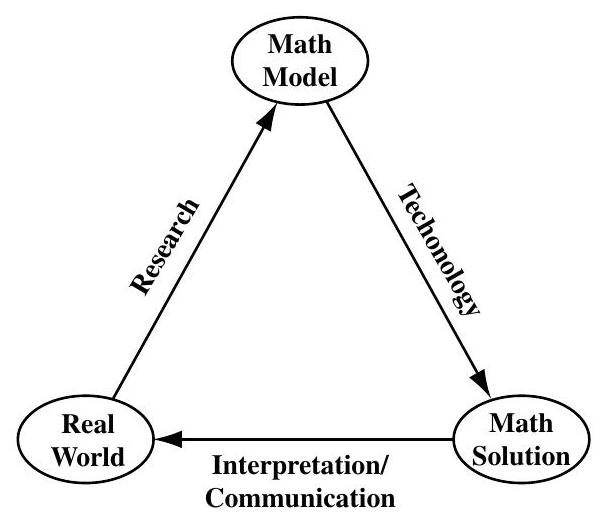
\includegraphics[max width=\textwidth]{2024_04_03_5bb5b4275a64cb9887d1g-028}
\end{center}

Fig. 2-1

\section*{QUALITATIVE METHODS}
To build a model can be a long and arduous process; it may take many years of research. Once they are formulated, models may be virtually impossible to solve analytically. Then the researcher has two options:

\begin{itemize}
  \item Simplify, or "tweak", the model so that it can be dealt with in a more manageable way. This is a valid approach, provided the simplification does not overly compromise the "real-world" connection, and therefore, its usefulness.
  \item Retain the model as is and use other techniques, such as numerical or graphical methods (see Chapter 18, Chapter 19, and Chapter 20). This represents a qualitative approach. While we do not possess an exact, analytical solution, we do obtain some information which can shed some light on the model and its application. Technological tools can be extremely helpful with this approach (see Appendix B).
\end{itemize}

\section*{Solved Problems}
Problems 2.1 through 2.11 deal with various models, many of which represent real-world situations. Assume the models are valid, even in the cases where some of the variables are discrete.

2.1. Discuss the model: $T_{F}=32+1.8 T_{C}$.

This model converts temperatures from degrees on the Celsius scale to degrees on the Fahrenheit scale.

2.2. Discuss the model: $P V=n R T$.

This models ideal gases and is known as the Perfect Gas Law. Here, $P$ is the pressure (in atmospheres), $V$ is the volume (liters), $n$ is the number of moles, $R$ is the universal gas constant $(R=8.3145 \mathrm{~J} / \mathrm{mol} \mathrm{K}$ ), and $T$ is the temperature (degrees Kelvin).

2.3. What does Boyle's law tell us?

Boyle's law states that, for an ideal gas at a constant temperature, $P V=k$, where $P$ (atmospheres), $V$ (liters) and $k$ is a constant (atmosphere-liters).

Another way of stating this, is that the pressure and volume are inversely proportional.

2.4. Discuss the model: $I=\frac{d q}{d t}$.

This formula is used in electricity; I represents the current (amperes), $q$ represents the charge (coulombs), $t$ is the time (seconds). Problems involving this model will be presented in both Chapter 7 and Chapter 14.

2.5. Discuss the model: $m \frac{d^{2} y}{d t^{2}}+a \frac{d y}{d t}+k y=F(t)$.

This is a classic model: a forced, mass-spring system. Here, $y$ is a displacement $(\mathrm{m}), t$ is time (sec), $m$ is the mass $(\mathrm{kg}), a$ is a friction or damping constant $(\mathrm{kg} / \mathrm{sec}), k$ is a spring constant $\left(\mathrm{kg} / \mathrm{sec}^{2}\right)$ and $F(t)$ is a forcing function $(\mathrm{N})$.

Variations of this model can be used in problems ranging from shock absorbers on an automobile to answering questions about the human spinal column.

The differential equation uses a number of classical concepts, including Newton's second law and Hooke's law. We will revisit this equation in Chapter 14.

2.6. Assume $M(t)$ represents the mass of an element in kgs. Suppose research has shown that the instantaneous rate of decay of this element $(\mathrm{kg} / \mathrm{yr})$ is proportional to the amount present: $M^{\prime}(t) \propto M(t)$. Set up a model for this relationship.

The proportionality relationship $M^{\prime}(t) \propto M(t)$ can be converted into an equation by introducing a proportionality constant, $k(1 / \mathrm{yr})$. So our model becomes $M^{\prime}(t)=k M(t)$. We note that $k<0$, because $M(t)$ is decreasing in size.

This equation will be classified as a "separable equation" (see Chapter 3). The solution to this differential equation, which is qualitatively described as "exponential decay", will be explored in Chapter 4.

2.7. Consider the previous problem. Assume research revealed that the rate of decay is proportional to the square root of the amount present. Model this situation. $M^{\prime}(t) \propto \sqrt{M(t)}$ implies $M^{\prime}(t)=k \sqrt{M(t)}$. We note here that the units of $k$ are $\frac{\mathrm{kg}^{1 / 2}}{\mathrm{yr}}$. The solution of this type\\
of differential equation will be explored in Chapter 4 .

2.8. Model a population $P(t)$, if its rate of growth is proportional to the amount present at time $t$.

This is the sister problem to Problem 2.6; that is, we have an "exponential growth" model, $P^{\prime}(t)=k P(t)$, where $k>0$.

2.9. Assume the population described in Problem 2.8 has an initial composition of 1000. That is, $P(0)=1000$. You are also told that the solution of the differential equation $P^{\prime}(t)=k P(t)$ is given by $P(t)=1000 e^{k t}$, where $t$ is in years. Discuss this model.

Since $k>0$, we know that $P(t)$ will increase exponentially as $t \rightarrow \infty$. We are forced to conclude that this is (most probably) not a reasonable model, due to the fact that our growth is unlimited.

We do add, however, that this model might be helpful over a short period of time. "How helpful?" and "How short a period?" are questions which must be looked at qualitatively, and depend on the constraints and requirements of the particular posed problem.

2.10. Consider the assumptions in the two previous problems. Further, suppose the rate of growth of $P(t)$ is proportional to the product of the amount present and some "maximum population" term, 100,000 $P(t)$, where the 100,000 represents the carrying capacity. That is, $P(t) \rightarrow 100,000$, as $t \rightarrow \infty$. Introduction of a proportionality constant $k$, leads to the differential equation, $P^{\prime}(t)=k P(t)(100,000-P(t))$. Discuss this model.

If $P(t)$ is much less than 100,000 , the differential equation can be approximated as $P^{\prime}(t) \approx k P(t)$ $(100,000)=K P(t)$, where $K=k(100,000)$. This would closely approximate exponential growth. So, for "small" $P(t)$, there would be little difference between this model and the previous model discussed in Problems 2.8 and 2.9.

If $P(t)$ is close to 100,000 (meaning that $100,000-P(t) \approx 0$ ), then the differential equation can be approximated as $P^{\prime}(t) \approx k P(t)(0)=0$. An approximate solution to this is $P(t)=100,000$, since only a constant has a derivative equal to 0 . So "in the large", $P(t)$ "levels off" to 100,000 , the carrying capacity of the population.

In this problem, we used a qualitative approach: we were able to decipher some information and express it in a descriptive way, even though we did not possess the solution to the differential equation. This type of equation is an example of a logistic population model and is used extensively in sociological studies. Also see Problem 7.7.

2.11. Sometimes differential equations are "coupled" (see Chapter 17 and Chapter 25); consider the following system:

\[
\left\{\begin{array}{l}
\frac{d R}{d t}=2 R-3 R F  \tag{1}\\
\frac{d F}{d t}=-4 F+5 R F
\end{array}\right.
\]

Here, let $R$ represent the number of rabbits in a population, while $F$ represents the number of foxes, and $t$ is time (months). Assume this model reflects the relationship between the rabbits and foxes. What does this model tell us?

This system of equations (I) mirrors a "predator-prey" relationship. The $R F$ terms in both equations can be interpreted as an "interaction term". That is, both factors are needed to have an effect on the equations.

We see that the coefficient of $R$ in the first equation is +2 ; if there was no $R F$ term in this equation, $R$ would increase without bound. The -3 coefficient of $R F$ has a negative impact on the rabbit population.

Turning our attention to the second equation, we see that $F$ is multiplied by a -4 , indicating that the fox population would decrease if they did not interact with rabbits. The positive coefficient for $R F$ indicates a positive impact on the fox population.

Predator-prey models are used extensively in many fields ranging from wildlife populations to military strategic planning. In many of these models qualitative methods are employed.

\section*{Supplementary Problems}
2.12. Using Problem 2.1. find a model which converts temperatures from degrees on the Fahrenheit scale to degrees on the Celsius scale. 2.13. Charles' law states that, for an ideal gas at a constant pressure, $\frac{V}{T}=k$, where $V$ (liters), $T$ (degrees Kelvin) and $k$ is\\
a constant $\left(\right.$ lit $\left./{ }^{\circ} K\right)$. What does this model tell us?

2.14. Discuss Newton's second law of motion: $F=m a=m \frac{d v}{d t}=m \frac{d^{2} x}{d t^{2}}$.

2.15. Suppose a room is being cooled according to the model $T(t)=\sqrt{576-t}$, where $t$ (hours) and $T$ (degrees Celsius). If we begin the cooling process at $t=0$, when will this model no longer hold? Why?

2.16. Suppose the room in Problem 2.15. was being cooled in such a way that $T(t)=t^{2}-20 t+\sqrt{576}$, where the variables and conditions are as above. How long would it take for the room to cool down to its minimum temperature? Why?

2.17. Consider the model discussed in Problem 2.5. If we assume that the system is both "undamped" and "unforced", that is $F(t) \equiv 0$ and $a=0$, the equation reduces to $m \frac{d^{2} y}{d t^{2}}+k y=0$. If we let $m=1$ and $k=4$ for further simplicity, we have $\frac{d^{2} y}{d t^{2}}+4 y=0$. Suppose we know that $y(t)=\sin 2 t$, satisfies the model. Describe the motion of displacement, $y(t)$.

2.18. Consider the previous problem. Find $(a)$ the velocity function; $(b)$ the acceleration function.

2.19. Consider the differential equation $\frac{d y}{d x}=(y-1)(y-2)$. Describe $(a)$ the behavior of $y$ at $y=1$ and $y=2 ;(b)$ what happens to $y$ if $y<1 ;(c)$ what happens to $y$ if $1<y<2 ;(d)$ what happens to $y$ if $y>2$.

2.20. Assume a chemical compound, $X$, is such that its rate of decay is proportional to the cube of its difference from a given amount, $M$, where both $X$ and $M$ are given in grams and time is measured in hours. Model this relationship with a differential equation.

2.21. Suppose $A$ and $B$ are two vats interconnected with a number of pipes and drains. If $A(t)$ and $B(t)$ represent the number of gallons of liquid sugar in the respective vats at time $t$ (hours), what do $A^{\prime}(t)$ and $B^{\prime}(t)$ represent?

2.22. Consider Problem 2.21. Suppose the following system of differential equations models the mixing of the vats:

\[
\left\{\begin{array}{l}
\frac{d A}{d t}=a A+b B+c  \tag{1}\\
\frac{d B}{d t}=d A+e B+f
\end{array}\right.
\]

where $a, b, c, d, e$, and $f$ are constants. What is happening to the liquid sugar and what are the units of the six constants?

\section*{CHAPTER 3 \\
 Differential Equations}
\section*{STANDARD FORM AND DIFFERENTIAL FORM}
Standard form for a first-order differential equation in the unknown function $y(x)$ is


\begin{equation*}
y^{\prime}=f(x, y) \tag{3.1}
\end{equation*}


where the derivative $y^{\prime}$ appears only on the left side of (3.1). Many, but not all, first-order differential equations can be written in standard form by algebraically solving for $y^{\prime}$ and then setting $f(x, y)$ equal to the right side of the resulting equation.

The right side of (3.1) can always be written as a quotient of two other functions $M(x, y)$ and $-N(x, y)$. Then (3.1) becomes $d y / d x=M(x, y) /-N(x, y)$, which is equivalent to the differential form


\begin{equation*}
M(x, y) d x+N(x, y) d y=0 \tag{3.2}
\end{equation*}


\section*{LINEAR EQUATIONS}
Consider a differential equation in standard form (3.1). If $f(x, y)$ can be written as $f(x, y)=-p(x) y+q(x)$ (that is, as a function of $x$ times $y$, plus another function of $x$ ), the differential equation is linear. First-order linear differential equations can always be expressed as


\begin{equation*}
y^{\prime}+p(x) y=q(x) \tag{3.3}
\end{equation*}


Linear equations are solved in Chapter 6.

\section*{BERNOULLI EQUATIONS}
A Bernoulli differential equation is an equation of the form


\begin{equation*}
y^{\prime}+p(x) y=q(x) y^{n} \tag{3.4}
\end{equation*}


where $n$ denotes a real number. When $n=1$ or $n=0$, a Bernoulli equation reduces to a linear equation. Bernoulli equations are solved in Chapter 6.

\section*{HOMOGENEOUS EQUATIONS}
A differential equation in standard form (3.1) is homogeneous if


\begin{equation*}
f(t x, t y)=f(x, y) \tag{3.5}
\end{equation*}


for every real number $t$. Homogeneous equations are solved in Chapter 4.

Note: In the general framework of differential equations, the word "homogeneous" has an entirely different meaning (see Chapter 8). Only in the context of first-order differential equations does "homogeneous" have the meaning defined above.

\section*{SEPARABLE EQUATIONS}
Consider a differential equation in differential form (3.2). If $M(x, y)=A(x)$ (a function only of $x$ ) and $N(x, y)=B(y)$ (a function only of $y$ ), the differential equation is separable, or has its variables separated. Separable equations are solved in Chapter 4.

\section*{EXACT EQUATIONS}
A differential equation in differential form (3.2) is exact if


\begin{equation*}
\frac{\partial M(x, y)}{\partial y}=\frac{\partial N(x, y)}{\partial x} \tag{3.6}
\end{equation*}


Exact equations are solved in Chapter 5 (where a more precise definition of exactness is given).

\section*{Solved Problems}
3.1. Write the differential equation $x y^{\prime}-y^{2}=0$ in standard form.

Solving for $y^{\prime}$, we obtain $y^{\prime}=y^{2} / x$ which has form (3.1) with $f(x, y)=y^{2} / x$.

3.2. Write the differential equation $e^{x} y^{\prime}+e^{2 x} y=\sin x$ in standard form.

Solving for $y^{\prime}$, we obtain

or

$$
\begin{aligned}
& e^{x} y^{\prime}=-e^{2 x} y+\sin x \\
& y^{\prime}=-e^{x} y+\mathrm{e}^{-x} \sin x
\end{aligned}
$$

which has form (3.1) with $f(x, y)=-e^{x} y+e^{-x} \sin x$.

3.3. Write the differential equation $\left(y^{\prime}+y\right)^{5}=\sin \left(y^{\prime} / x\right)$ in standard form.

This equation cannot be solved algebraically for $y^{\prime}$, and cannot be written in standard form.

3.4. Write the differential equation $y\left(y y^{\prime}-1\right)=x$ in differential form.

Solving for $y^{\prime}$, we have

$$
\begin{aligned}
y^{2} y^{\prime}-y & =x \\
y^{2} y^{\prime} & =x+y
\end{aligned}
$$


\begin{equation*}
y^{\prime}=\frac{x+y}{y^{2}} \tag{1}
\end{equation*}


which is in standard form with $f(x, y)=(x+y) / y^{2}$. There are infinitely many different differential forms associated with (1). Four such forms are:

(a) Take $M(x, y)=x+y, N(x, y)=-y^{2}$. Then

$$
\frac{M(x, y)}{-N(x, y)}=\frac{x+y}{-\left(-y^{2}\right)}=\frac{x+y}{y^{2}}
$$

and (1) is equivalent to the differential form

$$
(x+y) d x+\left(-y^{2}\right) d y=0
$$

(b) Take $M(x, y)=-1, N(x, y)=\frac{y^{2}}{x+y}$. Then

$$
\frac{M(x, y)}{-N(x, y)}=\frac{-1}{-y^{2} /(x+y)}=\frac{x+y}{y^{2}}
$$

and (1) is equivalent to the differential form

$$
(-1) d x+\left(\frac{y^{2}}{x+y}\right) d y=0
$$

(c) Take $M(x, y)=\frac{x+y}{2}, N(x, y)=\frac{-y^{2}}{2}$. Then

$$
\frac{M(x, y)}{-N(x, y)}=\frac{(x+y) / 2}{-\left(-y^{2} / 2\right)}=\frac{x+y}{y^{2}}
$$

and (1) is equivalent to the differential form

$$
\left(\frac{x+y}{2}\right) d x+\left(\frac{-y^{2}}{2}\right) d y=0
$$

(d) Take $M(x, y)=\frac{-x-y}{x^{2}}, N(x, y)=\frac{y^{2}}{x^{2}}$. Then

$$
\frac{M(x, y)}{-N(x, y)}=\frac{(-x-y) / x^{2}}{-y^{2} / x^{2}}=\frac{x+y}{y^{2}}
$$

and (1) is equivalent to the differential form

$$
\left(\frac{-x-y}{x^{2}}\right) d x+\left(\frac{y^{2}}{x^{2}}\right) d y=0
$$

3.5. Write the differential equation $d y / d x=y / x$ in differential form

This equation has infinitely many differential forms. One is

$$
d y=\frac{y}{x} d x
$$

which can be written in form (3.2) as


\begin{equation*}
\frac{y}{x} d x+(-1) d y=0 \tag{1}
\end{equation*}


Multiplying (1) through by $x$, we obtain


\begin{equation*}
y d x+(-x) d y=0 \tag{2}
\end{equation*}


as a second differential form. Multiplying (1) through by $1 / y$, we obtain


\begin{equation*}
\frac{1}{x} d x+\frac{-1}{y} d y=0 \tag{3}
\end{equation*}


as a third differential form. Still other differential forms are derived from (1) by multiplying that equation through by any other function of $x$ and $y$.

3.6. Write the differential equation $(x y+3) d x+\left(2 x-y^{2}+1\right) d y=0$ in standard form.

This equation is in differential form. We rewrite it as

$$
\left(2 x-y^{2}+1\right) d y=-(x y+3) d x
$$

which has the standard form

or

$$
\begin{aligned}
\frac{d y}{d x} & =\frac{-(x y+3)}{2 x-y^{2}+1} \\
y^{\prime} & =\frac{x y+3}{y^{2}-2 x-1}
\end{aligned}
$$

3.7. Determine if the following differential equations are linear:\\
(a) $y^{\prime}=(\sin x) y+e^{x}$\\
(b) $y^{\prime}=x \sin y+e^{x}$\\
(c) $y^{\prime}=5$\\
(d) $y^{\prime}=y^{2}+x$\\
(e) $y^{\prime}+x y^{5}=0$\\
(f) $x y^{\prime}+y=\sqrt{y}$\\
(g) $y^{\prime}+x y=e^{x} y$\\
(h) $y^{\prime}+\frac{x}{y}=0$\\
(a) The equation is linear; here $p(x)=-\sin x$ and $q(x)=e^{x}$.\\
(b) The equation is not linear because of the term $\sin y$.\\
(c) The equation is linear; here $p(x)=0$ and $q(x)=5$.\\
(d) The equation is not linear because of the term $y^{2}$.\\
(e) The equation is not linear because of the $y^{5}$ term.\\
(f) The equation is not linear because of the $y^{1 / 2}$ term.\\
(g) The equation is linear. Rewrite it as $y^{\prime}+\left(x-e^{x}\right) y=0$ with $p(x)=x-e^{x}$ and $q(x)=0$.\\
(h) The equation is not linear because of the $1 / y$ term.

3.8. Determine whether any of the differential equations in Problem 3.7 are Bernoulli equations.

All of the linear equations are Bernoulli equations with $n=0$. In addition, three of the nonlinear equations, $(e),(f)$ and $(h)$, are as well. Rewrite $(e)$ as $y^{\prime}=-x y^{5}$; it has form (3.4) with $p(x)=0, q(x)=-x$, and $n=5$. Rewrite $(f)$ as

$$
y^{\prime}+\frac{1}{x} y=\frac{1}{x} y^{1 / 2}
$$

It has form (3.4) with $p(x)=q(x)=1 / x$ and $n=1 / 2$. Rewrite $(h)$ as $y^{\prime}=-x y^{-1}$ with $p(x)=0, q(x)=-x$, and $n=-1$.

3.9. Determine if the following differential equations are homogeneous:\\
(a) $y^{\prime}=\frac{y+x}{x}$\\
(b) $y^{\prime}=\frac{y^{2}}{x}$\\
(c) $y^{\prime}=\frac{2 x y e^{x / y}}{x^{2}+y^{2} \sin \frac{x}{y}}$\\
(d) $y^{\prime}=\frac{x^{2}+y}{x^{3}}$\\
(a) The equation is homogeneous, since

$$
f(t x, t y)=\frac{t y+t x}{t x}=\frac{t(y+x)}{t x}=\frac{y+x}{x}=f(x, y)
$$

(b) The equation is not homogeneous, since

$$
f(t x, t y)=\frac{(t y)^{2}}{t x}=\frac{t^{2} y^{2}}{t x}=t \frac{y^{2}}{x} \neq f(x, y)
$$

(c) The equation is homogeneous, since

$$
\begin{aligned}
f(t x, t y) & =\frac{2(t x)(t y) e^{t x / t y}}{(t x)^{2}+(t y)^{2} \sin \frac{t x}{t y}}=\frac{t^{2} 2 x y e^{x / y}}{t^{2} x^{2}+t^{2} y^{2} \sin \frac{x}{y}} \\
& =\frac{2 x y e^{x / y}}{x^{2}+y^{2} \sin \frac{x}{y}}=f(x, y)
\end{aligned}
$$

(d) The equation is not homogeneous, since

$$
f(t x, t y)=\frac{(t x)^{2}+t y}{(t x)^{3}}=\frac{t^{2} x^{2}+t y}{t^{3} x^{3}}=\frac{t x^{2}+y}{t^{2} x^{3}} \neq f(x, y)
$$

3.10. Determine if the following differential equations are separable:\\
(a) $\sin x d x+y^{2} d y=0$\\
(b) $x y^{2} d x-x^{2} y^{2} d y=0$\\
(c) $(1+x y) d x+y d y=0$

(a) The differential equation is separable; here $M(x, y)=A(x)=\sin x$ and $N(x, y)=B(y)=y^{2}$.

(b) The equation is not separable in its present form, since $M(x, y)=x y^{2}$ is not a function of $x$ alone. But if we divide both sides of the equation by $x^{2} y^{2}$, we obtain the equation $(1 / x) d x+(-1) d y=0$, which is separable. Here, $A(x)=1 / x$ and $B(y)=-1$.

(c) The equation is not separable, since $M(x, y)=1+x y$, which is not a function of $x$ alone.

3.11. Determine whether the following differential equations are exact:\\
(a) $3 x^{2} y d x+\left(y+x^{3}\right) d y=0$\\
(b) $x y d x+y^{2} d y=0$

(a) The equation is exact; here $M(x, y)=3 x^{2} y, N(x, y)=y+x^{3}$, and $\partial M / \partial y=\partial N / \partial x=3 x^{2}$.

(b) The equation is not exact. Here $M(x, y)=x y$ and $N(x, y)=y^{2}$; hence $\partial M / \partial y=x, \partial N / \partial x=0$, and $\partial M / \partial y \neq \partial N / \partial x$.

3.12. Determine whether the differential equation $y^{\prime}=y / x$ is exact.

Exactness is only defined for equations in differential form, not standard form. The given differential equation has many differential forms. One such form is given in Problem 3.5, Eq. (1), as

$$
\frac{y}{x} d x+(-1) d y=0
$$

Here $M(x, y)=y / x, N(x, y)=-1$,

$$
\frac{\partial M}{\partial y}=\frac{1}{x} \neq 0=\frac{\partial N}{\partial x}
$$

and the equation is not exact. A second differential form for the same differential equation is given in Eq. (3) of Problem 3.5 as

$$
\frac{1}{x} d x+\frac{-1}{y} d y=0
$$

Here $M(x, y)=1 / x, N(x, y)=-1 / y$,

$$
\frac{\partial M}{\partial y}=0=\frac{\partial N}{\partial x}
$$

and the equation is exact. Thus, a given differential equation has many differential forms, some of which may be exact.

3.13. Prove that a separable equation is always exact.

For a separable differential equation, $M(x, y)=A(x)$ and $N(x, y)=B(y)$. Thus,

$$
\frac{\partial M(x, y)}{\partial y}=\frac{\partial A(x)}{\partial y}=0 \quad \text { and } \quad \frac{\partial N(x, y)}{\partial x}=\frac{\partial B(y)}{\partial x}=0
$$

Since $\partial M / \partial y=\partial N / \partial x$, the differential equation is exact.

3.14. A theorem of first-order differential equations states that if $f(x, y)$ and $\partial f(x, y) / \partial y$ are continuous in a rectangle $\mathscr{R}:\left|x-x_{0}\right| \leq a,\left|y-y_{0}\right| \leq b$, then there exists an interval about $x_{0}$ in which the initial-value problem $y^{\prime}=f(x, y) ; y\left(x_{0}\right)=y_{0}$ has a unique solution. The initial-value problem $y^{\prime}=2 \sqrt{|y|} ; y(0)=0$ has the two solutions $y=x|x|$ and $y \equiv 0$. Does this result violate the theorem?

No. Here, $f(x, y)=2 \sqrt{|y|}$ and, therefore, $\partial f / \partial y$ does not exist at the origin.

\section*{Supplementary Problems}
In Problems 3.15 through 3.25, write the given differential equations in standard form.\\
3.15. $x y^{\prime}+y^{2}=0$\\
3.16. $e^{x} y^{\prime}-x=y^{\prime}$\\
3.17. $\left(y^{\prime}\right)^{3}+y^{2}+y=\sin x$\\
3.18. $x y^{\prime}+\cos \left(y^{\prime}+y\right)=1$\\
3.19. $e^{\left(y^{\prime}+y\right)}=x$\\
3.20. $\left(y^{\prime}\right)^{2}-5 y^{\prime}+6=(x+y)\left(y^{\prime}-2\right)$\\
3.21. $(x-y) d x+y^{2} d y=0$\\
3.22. $\frac{x+y}{x-y} d x-d y=0$\\
3.23. $d x+\frac{x+y}{x-y} d y=0$\\
3.24. $\left(e^{2 x}-y\right) d x+e^{x} d y=0$

3.25. $d y+d x=0$

In Problems 3.26 through 3.35, differential equations are given in both standard and differential form. Determine whether the equations in standard form are homogeneous and/or linear, and, if not linear, whether they are Bernoulli; determine whether the equations in differential form, as given, are separable and/or exact.

3.26. $\quad y^{\prime}=x y ; \quad x y d x-d y=0$

3.27. $y^{\prime}=x y ; \quad x d x-\frac{1}{y} d y=0$

3.28. $y^{\prime}=x y+1 ; \quad(x y+1) d x-d y=0$

3.29. $y^{\prime}=\frac{x^{2}}{y^{2}} ; \quad \frac{x^{2}}{y^{2}} d x-d y=0$

3.30. $y^{\prime}=\frac{x^{2}}{y^{2}} ; \quad-x^{2} d x+y^{2} d y=0$

3.31. $y^{\prime}=-\frac{2 y}{x} ; \quad 2 x y d x+x^{2} d y=0$

3.32. $y^{\prime}=\frac{x y^{2}}{x^{2} y+y^{3}} ; \quad x y^{2} d x-\left(x^{2} y+y^{3}\right) d y=0$

3.33. $y^{\prime}=\frac{-x y^{2}}{x^{2} y+y^{2}} ; \quad x y^{2} d x+\left(x^{2} y+y^{2}\right) d y=0$

3.34. $\quad y^{\prime}=x^{3} y+x y^{3} ; \quad\left(x^{2}+y^{2}\right) d x-\frac{1}{x y} d y=0$

3.35. $y^{\prime}=2 x y+x ; \quad\left(2 x y e^{-x^{2}}+x e^{-x^{2}}\right) d x-e^{-x^{2}} d y=0$

\section*{CHAPTER 4}
\section*{Separable First-Order Differential Equations}
\section*{GENERAL SOLUTION}
The solution to the first-order separable differential equation (see Chapter 3)


\begin{gather*}
A(x) d x+B(y) d y=0  \tag{4.1}\\
\int A(x) d x+\int B(y) d y=c \tag{4.2}
\end{gather*}


where $c$ represents an arbitrary constant.

The integrals obtained in Eq. (4.2) may be, for all practical purposes, impossible to evaluate. In such cases, numerical techniques (see Chapters $18,19,20$ ) are used to obtain an approximate solution. Even if the indicated integrations in (4.2) can be performed, it may not be algebraically possible to solve for $y$ explicitly in terms of $x$. In that case, the solution is left in implicit form.

\section*{SOLUTIONS TO THE INITIAL-VALUE PROBLEM}
The solution to the initial-value problem


\begin{equation*}
A(x) d x+B(y) d y=0 ; \quad y\left(x_{0}\right)=y_{0} \tag{4.3}
\end{equation*}


can be obtained, as usual, by first using Eq. (4.2) to solve the differential equation and then applying the initial condition directly to evaluate $c$.

Alternatively, the solution to Eq. (4.3) can be obtained from


\begin{equation*}
\int_{x_{0}}^{x} A(x) d x+\int_{y_{0}}^{y} B(y) d y=0 \tag{4.4}
\end{equation*}


Equation (4.4), however, may not determine the solution of (4.3) uniquely; that is, (4.4) may have many solutions, of which only one will satisfy the initial-value problem.

\section*{REDUCTION OF HOMOGENEOUS EQUATIONS}
The homogeneous differential equation


\begin{equation*}
\frac{d y}{d x}=f(x, y) \tag{4.5}
\end{equation*}


having the property that $f(t x, t y)=f(x, y)$ (see Chapter 3 ) can be transformed into a separable equation by making the substitution


\begin{equation*}
y=x v \tag{4.6}
\end{equation*}


along with its corresponding derivative


\begin{equation*}
\frac{d y}{d x}=v+x \frac{d v}{d x} \tag{4.7}
\end{equation*}


The resulting equation in the variables $v$ and $x$ is solved as a separable differential equation; the required solution to Eq. (4.5) is obtained by back substitution.

Alternatively, the solution to (4.5) can be obtained by rewriting the differential equation as


\begin{equation*}
\frac{d x}{d y}=\frac{1}{f(x, y)} \tag{4.8}
\end{equation*}


and then substituting


\begin{equation*}
x=y u \tag{4.9}
\end{equation*}


and the corresponding derivative


\begin{equation*}
\frac{d x}{d y}=u+y \frac{d u}{d y} \tag{4.10}
\end{equation*}


into Eq. (4.8). After simplifying, the resulting differential equation will be one with variables (this time, $u$ and $y$ ) separable.

Ordinarily, it is immaterial which method of solution is used (see Problems 4.12 and 4.13). Occasionally, however, one of the substitutions (4.6) or (4.9) is definitely superior to the other one. In such cases, the better substitution is usually apparent from the form of the differential equation itself. (See Problem 4.17.)

\section*{Solved Problems}
4.1. Solve $x d x-y^{2} d y=0$.

For this differential equation, $A(x)=x$ and $B(y)=-y^{2}$. Substituting these values into Eq. (4.2), we have

$$
\int x d x+\int\left(-y^{2}\right) d y=c
$$

which, after the indicated integrations are performed, becomes $x^{2} / 2-y^{3} / 3=c$. Solving for $y$ explicitly, we obtain the solution as

$$
y=\left(\frac{3}{2} x^{2}+k\right)^{1 / 3} ; \quad k=-3 c
$$

4.2. Solve $y^{\prime}=y^{2} x^{3}$.

We first rewrite this equation in the differential form (see Chapter 3) $x^{3} d x-\left(1 / y^{2}\right) d y=0$. Then $A(x)=x^{3}$ and $B(y)=-1 / y^{2}$. Substituting these values into Eq. (4.2), we have

$$
\int x^{3} d x+\int\left(-1 / y^{2}\right) d y=c
$$

or, by performing the indicated integrations, $x^{4} / 4+1 / y=c$. Solving explicitly for $y$, we obtain the solution as

$$
y=\frac{-4}{x^{4}+k}, \quad k=-4 c
$$

4.3. Solve $\frac{d y}{d x}=\frac{x^{2}+2}{y}$

This equation may be rewritten in the differential form

$$
\left(x^{2}+2\right) d x-y d y=0
$$

which is separable with $A(x)=x^{2}+2$ and $B(y)=-y$. Its solution is

or

$$
\begin{gathered}
\int\left(x^{2}+2\right) d x-\int y d y=c \\
\frac{1}{3} x^{3}+2 x-\frac{1}{2} y^{2}=c
\end{gathered}
$$

Solving for $y$, we obtain the solution in implicit form as

$$
y^{2}=\frac{2}{3} x^{3}+4 x+k
$$

with $k=-2 c$. Solving for $y$ implicitly, we obtain the two solutions

$$
y=\sqrt{\frac{2}{3} x^{3}+4 x+k} \quad \text { and } \quad y=-\sqrt{\frac{2}{3} x^{3}+4 x+k}
$$

4.4. Solve $y^{\prime}=5 y$.

First rewrite this equation in the differential form $5 d x-(1 / y) d y=0$, which is separable. Its solution is

$$
\int 5 d x+\int(-1 / y) d y=c
$$

or, by evaluating, $5 x-\ln |y|=c$.

To solve for $y$ explicitly, we first rewrite the solution as $\ln |y|=5 x-c$ and then take the exponential of both sides. Thus, $e^{\ln |y|}=e^{5 x-c}$. Noting that $e^{\ln |y|}=|y|$, we obtain $|y|=e^{5 x} e^{-c}$, or $y= \pm e^{-c} e^{5 x}$. The solution is given explicitly by $y=k e^{5 x}, k= \pm e^{-c}$.

Note that the presence of the term $(-1 / y)$ in the differential form of the differential equation requires the restriction $y \neq 0$ in our derivation of the solution. This restriction is equivalent to the restriction $k \neq 0$, since $y=k e^{5 x}$. However, by inspection, $y \equiv 0$ is a solution of the differential equation as originally given. Thus, $y=k e^{5 x}$ is the solution for all $k$.

The differential equation as originally given is also linear. See Problem 6.9 for an alternate method of solution.

4.5. Solve $y^{\prime}=\frac{x+1}{y^{4}+1}$.

This equation, in differential form, is $(x+1) d x+\left(-y^{4}-1\right) d y=0$, which is separable. Its solution is

$$
\int(x+1) d x+\int\left(-y^{4}-1\right) d y=c
$$

or, by evaluating,

$$
\frac{x^{2}}{2}+x-\frac{y^{5}}{5}-y=c
$$

Since it is impossible algebraically to solve this equation explicitly for $y$, the solution must be left in its present implicit form.

4.6. Solve $d y=2 t\left(y^{2}+9\right) d t$.

This equation may be rewritten as

$$
\frac{d y}{y^{2}+9}-2 t d t=0
$$

which is separable in variables $y$ and $t$. Its solution is

$$
\int \frac{d y}{y^{2}+9}-\int 2 t d t=c
$$

or, upon evaluating the given integrals,

$$
\frac{1}{3} \arctan \left(\frac{y}{3}\right)-t^{2}=c
$$

Solving for $y$, we obtain

or

$$
\begin{aligned}
& \arctan \left(\frac{y}{3}\right)=3\left(t^{2}+c\right) \\
& \frac{y}{3}=\tan \left(3 t^{2}+3 c\right) \\
& y=3 \tan \left(3 t^{2}+\mathrm{k}\right)
\end{aligned}
$$

with $k=3 c$.

4.7. Solve $\frac{d x}{d t}=x^{2}-2 x+2$.

This equation may be rewritten in differential form

$$
\frac{d x}{x^{3}-2 x+2}-d t=0
$$

which is separable in the variables $x$ and $t$. Its solution is

$$
\int \frac{d x}{x^{3}-2 x+2}-\int d t=c
$$

Evaluating the first integral by first completing the square, we obtain

or

$$
\begin{gathered}
\int \frac{d x}{(x-1)^{2}+1}-\int d t=c \\
\arctan (x-1)-t=c
\end{gathered}
$$

Solving for $x$ as a function of $t$, we obtain

$$
\begin{aligned}
\arctan & (x-1)=t+c \\
x-1 & =\tan (t+c) \\
x & =1+\tan (t+c)
\end{aligned}
$$

4.8. Solve $e^{x} d x-y d y=0 ; y(0)=1$.

The solution to the differential equation is given by Eq. (4.2) as

$$
\int e^{x} d x+\int(-y) d y=c
$$

or, by evaluating, as $y^{2}=2 e^{x}+k, k=-2 c$. Applying the initial condition, we obtain $(1)^{2}=2 e^{0}+k, 1=2+k$, or $k=-1$. Thus, the solution to the initial-value problem is

$$
y^{2}=2 e^{x}-1 \quad \text { or } \quad y=\sqrt{2 e^{x}-1}
$$

[Note that we cannot choose the negative square root, since then $y(0)=-1$, which violates the initial condition.]

To ensure that $y$ remains real, we must restrict $x$ so that $2 e^{x}-1 \geq 0$. To guarantee that $y^{\prime}$ exists [note that $\left.y^{\prime}(x)=d y / d x=e^{x} / y\right]$, we must restrict $x$ so that $2 e^{x}-1 \neq 0$. Together these conditions imply that $2 e^{x}-1>0$, or $x>\ln \frac{1}{2}$.

4.9. Use Eq. (4.4) to solve Problem 4.8.

For this problem, $x_{0}=0, y_{0}=1, A(x)=e^{x}$, and $B(y)=-y$. Substituting these values into Eq. (4.4), we obtain

$$
\int_{0}^{x} e^{x} d x+\int_{1}^{y}(-y) d y=0
$$

Evaluating these integrals, we have

$$
\left.e^{x}\right|_{0} ^{x}+\left.\left(\frac{-y^{2}}{2}\right)\right|_{1} ^{y}=0 \quad \text { or } \quad e^{x}-e^{0}+\left(\frac{-y^{2}}{2}\right)-\left(-\frac{1}{2}\right)=0
$$

Thus, $y^{2}=2 e^{x}-1$, and, as in Problem 4.8, $y=\sqrt{2 e^{x}-1}, \quad x>\ln \frac{1}{2}$.

4.10. Solve $x \cos x d x+\left(1-6 y^{5}\right) d y=0 ; y(\pi)=0$.

Here, $x_{0}=\pi, y_{0}=0, A(x)=x \cos x$, and $B(y)=1-6 y^{5}$. Substituting these values into Eq. (4.4), we obtain

$$
\int_{\pi}^{x} x \cos x d x+\int_{0}^{y}\left(1-6 y^{5}\right) d y=0
$$

Evaluating these integrals (the first one by integration by parts), we find

or

$$
\begin{gathered}
\left.x \sin x\right|_{\pi} ^{x}+\left.\cos x\right|_{\pi} ^{x}+\left.\left(y-y^{6}\right)\right|_{0} ^{y}=0 \\
x \sin x+\cos x+1=y^{6}-y
\end{gathered}
$$

Since we cannot solve this last equation for $y$ explicitly, we must be content with the solution in its present implicit form.

4.11. Solve $y^{\prime}=\frac{y+x}{x}$.

This differential equation is not separable, but it is homogeneous as shown in Problem 3.9(a). Substituting Eqs. (4.6) and (4.7) into the equation, we obtain

$$
v+x \frac{d v}{d x}=\frac{x v+x}{x}
$$

which can be algebraically simplified to

$$
x \frac{d v}{d x}=1 \quad \text { or } \quad \frac{1}{x} d x-d v=0
$$

This last equation is separable; its solution is

$$
\int \frac{1}{x} d x-\int d v=c
$$

which, when evaluated, yields $v=\ln |x|-c$, or


\begin{equation*}
v=\ln |k x| \tag{1}
\end{equation*}


where we have set $c=-\ln |k|$ and have noted that $\ln |x|+\ln |k|=\ln |k x|$. Finally, substituting $v=y / x$ back into (1), we obtain the solution to the given differential equation as $y=x \ln |k x|$.

4.12. Solve $y^{\prime}=\frac{2 y^{4}+x^{4}}{x y^{3}}$.

This differential equation is not separable. Instead it has the form $y^{\prime}=f(x, y)$, with

where

$$
\begin{gathered}
f(x, y)=\frac{2 y^{4}+x^{4}}{x y^{3}} \\
f(t x, t y)=\frac{2(t y)^{4}+(t x)^{4}}{(t x)(t y)^{3}}=\frac{t^{4}\left(2 y^{4}+x^{4}\right)}{t^{4}\left(x y^{3}\right)}=\frac{2 y^{4}+x^{4}}{x y^{3}}=f(x, y)
\end{gathered}
$$

so it is homogeneous. Substituting Eqs. (4.6) and (4.7) into the differential equation as originally given, we obtain

$$
v+x \frac{d v}{d x}=\frac{2(x v)^{4}+x^{4}}{x(x v)^{3}}
$$

which can be algebraically simplified to

$$
x \frac{d v}{d x}=\frac{v^{4}+1}{v^{3}} \quad \text { or } \quad \frac{1}{x} d x-\frac{v^{3}}{v^{4}+1} d v=0
$$

This last equation is separable; its solution is

$$
\int \frac{1}{x} d x-\int \frac{v^{3}}{v^{4}+1} d v=c
$$

Integrating, we obtain in $\ln |x|-\frac{1}{4} \ln \left(v^{4}+1\right)=c$, or


\begin{equation*}
v^{4}+1=(k x)^{4} \tag{1}
\end{equation*}


where we have set $c=-\ln |k|$ and then used the identities

$$
\ln |x|+\ln |k|=\ln |k x| \quad \text { and } \quad 4 \ln |k x|=\ln (k x)^{4}
$$

Finally, substituting $v=y / x$ back into (1), we obtain


\begin{equation*}
y^{4}=c_{1} x^{8}-x^{4} \quad\left(c_{1}=k^{4}\right) \tag{2}
\end{equation*}


4.13. Solve the differential equation of Problem 4.12 by using Eqs. (4.9) and (4.10).

We first rewrite the differential equation as

$$
\frac{d x}{d y}=\frac{x y^{3}}{2 y^{4}+x^{4}}
$$

Then substituting (4.9) and (4.10) into this new differential equation, we obtain

$$
u+y \frac{d u}{d y}=\frac{(y u) y^{3}}{2 y^{4}+(y u)^{4}}
$$

which can be algebraically simplified to

or


\begin{gather*}
y \frac{d u}{d y}=-\frac{u+u^{5}}{2+u^{4}} \\
\frac{1}{y} d y+\frac{2+u^{4}}{u+u^{5}} d u=0 \tag{1}
\end{gather*}


Equation (1) is separable; its solution is

$$
\int \frac{1}{y} d y+\int \frac{2+u^{4}}{u+u^{5}} d u=c
$$

The first integral is in ln $|y|$. To evaluate the second integral, we use partial fractions on the integrand to obtain

$$
\frac{2+u^{4}}{u+u^{5}}=\frac{2+u^{4}}{u\left(1+u^{4}\right)}=\frac{2}{u}-\frac{u^{3}}{1+u^{4}}
$$

Therefore,

$$
\int \frac{2+u^{4}}{u+u^{5}} d u=\int \frac{2}{u} d u-\int \frac{u^{3}}{1+u^{4}} d u=2 \ln |u|-\frac{1}{4} \ln \left(1+u^{4}\right)
$$

The solution to (1) is in $\ln |y|+2 \ln |u|-\frac{1}{4} \ln \left(1+u^{4}\right)=c$, which can be rewritten as


\begin{equation*}
k y^{4} u^{8}=1+u^{4} \tag{2}
\end{equation*}


where $c=-\frac{1}{4} \ln |k|$. Substituting $u=x / y$ back into (2), we once again have (2) of Problem 4.12.

4.14. Solve $y^{\prime}=\frac{2 x y}{x^{2}-y^{2}}$.

This differential equation is not separable. Instead it has the form $y^{\prime}=f(x, y)$, with

$$
f(x, y)=\frac{2 x y}{x^{2}-y^{2}}
$$

where

$$
f(t x, t y)=\frac{2(t x)(t y)}{(t x)^{2}-(t y)^{2}}=\frac{t^{2}(2 x y)}{t^{2}\left(x^{2}-y^{2}\right)}=\frac{2 x y}{x^{2}-y^{2}}=f(x, y)
$$

so it is homogenous. Substituting Eqs. (4.6) and (4.7) into the differential equation as originally given, we obtain

$$
v+x \frac{d v}{d x}=\frac{2 x(x v)}{x^{2}-(x v)^{2}}
$$

which can be algebraically simplified to

or


\begin{gather*}
x \frac{d v}{d x}=-\frac{v\left(v^{2}+1\right)}{v^{2}-1} \\
\frac{1}{x} d x+\frac{v^{2}-1}{v\left(v^{2}+1\right)} d v=0 \tag{1}
\end{gather*}


Using partial fractions, we can expand (1) to


\begin{equation*}
\frac{1}{x} d x+\left(-\frac{1}{v}+\frac{2 v}{v^{2}+1}\right) d v=0 \tag{2}
\end{equation*}


The solution to this separable equation is found by integrating both sides of (2). Doing so, we obtain $\ln |x|-$ $\ln |v|+\ln \left(v^{2}+1\right)=c$, which can be simplified to


\begin{equation*}
x\left(v^{2}+1\right)=k v \quad(c=1 \mathrm{n}|k|) \tag{3}
\end{equation*}


Substituting $v=y / x$ into (3), we find the solution of the given differential equation is $x^{2}+y^{2}=k y$.

4.15. Solve $y^{\prime}=\frac{x^{2}+y^{2}}{x y}$.

This differential equation is homogeneous. Substituting Eqs. (4.6) and (4.7) into it, we obtain

$$
v+x \frac{d v}{d x}=\frac{x^{2}+(x v)^{2}}{x(x v)}
$$

which can be algebraically simplified to

$$
x \frac{d v}{d x}=\frac{1}{v} \quad \text { or } \quad \frac{1}{x} d x-v d v=0
$$

The solution to this separable equation is $\ln |x|-v^{2} / 2=c$, or equivalently


\begin{equation*}
v^{2}=\ln x^{2}+k \quad(k=-2 c) \tag{1}
\end{equation*}


Substituting $v=y / x$ into (1), we find that the solution to the given differential equation is

$$
y^{2}=x^{2} \ln x^{2}+k x^{2}
$$

4.16. Solve $y^{\prime}=\frac{x^{2}+y^{2}}{x y} ; \quad y(1)=-2$.

The solution to the differential equation is given in Problem 3.15 as $y^{2}=x^{2} \ln x^{2}+k x^{2}$. Applying the initial condition, we obtain $(-2)^{2}=(1)^{2} \ln (1)^{2}+k(1)^{2}$, or $k=4$. (Recall that $\ln 1=0$.) Thus, the solution to the initial-value problem is

$$
y^{2}=x^{2} \ln x^{2}+4 x^{2} \quad \text { or } \quad y=-\sqrt{x^{2} \ln x^{2}+4 x^{2}}
$$

The negative square root is taken, to be consistent with the initial condition.

4.17. Solve $y^{\prime}=\frac{2 x y e^{(x / y)^{2}}}{y^{2}+y^{2} e^{(x / y)^{2}}+2 x^{2} e^{(x / y)^{2}}}$.

This differential equation is not separable, but it is homogeneous. Noting the $(x / y)$-term in the exponential, we try the substitution $u=x / y$, which is an equivalent form of (4.9). Rewriting the differential equation as

$$
\frac{d x}{d y}=\frac{y^{2}+y^{2} e^{(x / y)^{2}}+2 x^{2} e^{(x / y)^{2}}}{2 x y e^{(x / y)^{2}}}
$$

we have upon using substitutions (4.9) and (4.10) and simplifying,

$$
y \frac{d u}{d y}=\frac{1+e^{u^{2}}}{2 u e^{u^{2}}} \quad \text { or } \quad \frac{1}{y} d y-\frac{2 u e^{u^{2}}}{1+e^{u^{2}}} d u=0
$$

This equation is separable; its solution is

$$
\ln |y|-\ln \left(1+e^{u^{2}}\right)=c
$$

which can be rewritten as


\begin{equation*}
y=k\left(1+e^{u^{2}}\right) \quad(c=\ln |k|) \tag{1}
\end{equation*}


Substituting $u=x / y$ into (1), we obtain the solution of the given differential equation as

$$
y=k\left[1+e^{(x / y)^{2}}\right]
$$

4.18. Prove that every solution of Eq. (4.2) satisfies Eq. (4.1).

Rewrite (4.1) as $A(x)+B(y) y^{\prime}=0$. If $y(x)$ is a solution, it must satisfy this equation identically in $x$; hence,

$$
A(x)+B\lfloor y(x)] y^{\prime}(x)=0
$$

Integrating both sides of this last equation with respect to $x$, we obtain

$$
\int A(x) d x+\int B[y(x)] y^{\prime}(x) d x=c
$$

In the second integral, make the change of variables $y=y(x)$, hence $d y=y^{\prime}(x) d x$. The result of this substitution is (4.2).

4.19. Prove that every solution of system (4.3) is a solution of (4.4).

Following the same reasoning as in Problem 4.18, except now integrating from $x=x_{0}$ to $x=x$, we obtain

$$
\int_{x_{0}}^{x} A(x) d x+\int_{x_{0}}^{x} B[y(x)] y^{\prime}(x) d x=0
$$

The substitution $y=y(x)$ again gives the desired result. Note that as $x$ varies from $x_{0}$ to $x, y$ will vary from $y\left(x_{0}\right)=y_{0}$ to $y(x)=y$.

4.20. Prove that if $y^{\prime}=f(x, y)$ is homogeneous, then the differential equation can be rewritten as $y^{\prime}=g(y / x)$, where $g(y / x)$ depends only on the quotient $y / x$.

We have that $f(x, y)=f(t x, t y)$. Since this equation is valid for all $t$, it must be true, in particular, for $t=1 / x$. Thus, $f(x, y)=f(1, y / x)$. If we now define $g(y / x)=f(1, y / x)$, we then have $y^{\prime}=f(x, y)=f(1, y / x)=g(y / x)$ as required.

Note that this form suggests the substitution $v=y / x$ which is equivalent to (4.6). If, in the above, we had set $t=1 / y$, then $f(x, y)=f(x / y, 1)=h(x / y)$, which suggests the alternate substitution (4.9).

4.21. A function $g(x, y)$ is homogeneous of degree $n$ if $g(t x, t y)=t^{n} g(x, y)$ for all $t$. Determine whether the following functions are homogeneous, and, if so, find their degree:

(a) $x y+y^{2}, \quad$ (b) $x+y \sin (y / x)^{2}, \quad$ (c) $x^{3}+x y^{2} \mathrm{e}^{x / y}$, and (d) $x+x y$.

(a) $(t x)(t y)+(t y)^{2}=t^{2}\left(x y+y^{2}\right)$; homogeneous of degree two.

(b) $t x+t y \sin \left(\frac{t y}{t x}\right)^{2}=t\left[x+y \sin \left(\frac{y}{x}\right)^{2}\right]$; homogeneous of degree one.

(c) $(t x)^{3}+(t x)(t y)^{2} e^{t x / t y}=t^{3}\left(x^{3}+x y^{2} e^{x / y}\right)$; homogeneous of degree three.

(d) $t x+(t x)(t y)=t x+t^{2} x y$; not homogeneous.

4.22. An alternate definition of a homogeneous differential equation is as follows: A differential equation $M(x, y) d x+N(x, y) d y=0$ is homogenous if both $M(x, y)$ and $N(x, y)$ are homogeneous of the same degree (see Problem 4.21). Show that this definition implies the definition given in Chapter 3.

If $M(x, y)$ and $N(x, y)$ are homogeneous of degree $n$, then

$$
f(t x, t y)=\frac{M(t x, t y)}{-N(t x, t y)}=\frac{t^{n} M(x, y)}{-t^{n} N(x, y)}=\frac{M(x, y)}{-N(x, y)}=f(x, y)
$$

\section*{Supplementary Problems}
In Problems 4.23 through 4.45, solve the given differential equations or initial-value problems.\\
4.23. $x d x+y d y=0$\\
4.24. $x d x-y^{3} d y=0$\\
4.25. $d x+\frac{1}{y^{4}} d y=0$\\
4.26. $(t+1) d t-\frac{1}{y^{2}} d y=0$

4.27. $\frac{1}{x} d x-\frac{1}{y} d y=0$

4.29. $x d x+\frac{1}{y} d y=0$

4.31. $\frac{4}{t} d t-\frac{y-3}{y} d y=0$

4.33. $d x-\frac{1}{y^{2}-6 y+13} d y=0$

4.35. $y^{\prime}=\frac{x e^{x}}{2 y}$

4.37. $\frac{d y}{d x}=y^{2}$

4.39. $\frac{d x}{d t}=\frac{x}{t}$

4.41. $\sin x d x+y d y=0 ; \quad y(0)=-2$

4.43. $x e^{x^{2}} d x+\left(y^{5}-1\right) d y=0 ; \quad y(0)=0$

4.45. $\frac{d x}{d t}=8-3 x ; \quad x(0)=4$

In Problems 4.46 through 4.54, determine whether the given differential equations are homogenous and, if so, solve them.\\
4.46. $y^{\prime}=\frac{y-x}{x}$\\
4.47. $y^{\prime}=\frac{2 y+x}{x}$\\
4.48. $y^{\prime}=\frac{x^{2}+2 y^{2}}{x y}$\\
4.49. $y^{\prime}=\frac{2 x+y^{2}}{x y}$\\
4.50. $y^{\prime}=\frac{x^{2}+y^{2}}{2 x y}$\\
4.51. $y^{\prime}=\frac{2 x y}{y^{2}-x^{2}}$\\
4.52. $y^{\prime}=\frac{y}{x+\sqrt{x y}}$\\
4.53. $y^{\prime}=\frac{y^{2}}{x y+\left(x y^{2}\right)^{1 / 3}}$\\
4.54. $y^{\prime}=\frac{x^{4}+3 x^{2} y^{2}+y^{4}}{x^{3} y}$

\begin{center}

\includegraphics[max width=\textwidth]{2024_04_03_5bb5b4275a64cb9887d1g-049}
\end{center}

\section*{Differential Equations}
\section*{DEFINING PROPERTIES}
A differential equation


\begin{equation*}
M(x, y) d x+N(x, y) d y=0 \tag{5.1}
\end{equation*}


is exact if there exists a function $g(x, y)$ such that


\begin{equation*}
d g(x, y)=M(x, y) d x+N(x, y) d y \tag{5.2}
\end{equation*}


Test for exactness: If $M(x, y)$ and $N(x, y)$ are continuous functions and have continuous first partial derivatives on some rectangle of the $x y$-plane, then (5.1) is exact if and only if


\begin{equation*}
\frac{\partial M(x, y)}{\partial y}=\frac{\partial N(x, y)}{\partial x} \tag{5.3}
\end{equation*}


\section*{METHOD OF SOLUTION}
To solve Eq. (5.1), assuming that it is exact, first solve the equations


\begin{align*}
& \frac{\partial g(x, y)}{\partial x}=M(x, y)  \tag{5.4}\\
& \frac{\partial g(x, y)}{\partial y}=N(x, y) \tag{5.5}
\end{align*}


for $g(x, y)$. The solution to (5.1) is then given implicitly by


\begin{equation*}
g(x, y)=\mathrm{c} \tag{5.6}
\end{equation*}


where $c$ represents an arbitrary constant.

Equation (5.6) is immediate from Eqs. (5.1) and (5.2). If (5.2) is substituted into (5.1), we obtain $d g(x, y(x))=0$. Integrating this equation (note that we can write 0 as $0 d x$ ), we have $\int d g(x, y(x))=\int 0 d x$, which, in turn, implies (5.6).

\section*{INTEGRATING FACTORS}
In general, Eq. (5.1) is not exact. Occasionally, it is possible to transform (5.1) into an exact differential equation by a judicious multiplication. A function $I(x, y)$ is an integrating factor for $(5.1)$ if the equation


\begin{equation*}
I(x, y)[M(x, y) d x+N(x, y) d y]=0 \tag{5.7}
\end{equation*}


is exact. A solution to (5.1) is obtained by solving the exact differential equation defined by (5.7). Some of the more common integrating factors are displayed in Table 5-1 and the conditions that follow:

If $\frac{1}{N}\left(\frac{\partial M}{\partial y}-\frac{\partial N}{\partial x}\right) \equiv g(x)$, a function of $x$ alone, then


\begin{equation*}
I(x, y)=e^{\int g(x) d x} \tag{5.8}
\end{equation*}


If $\frac{1}{M}\left(\frac{\partial M}{\partial y}-\frac{\partial N}{\partial x}\right) \equiv h(y)$, a function of $y$ alone, then


\begin{equation*}
I(x, y)=e^{-\int h(y) d y} \tag{5.9}
\end{equation*}


Table 5-1

\begin{center}
\begin{tabular}{|c|c|c|}
\hline
Group of terms & Integrating factor $I(x, y)$ & Exact differential $d g(x, y)$ \\
\hline
$y d x-x d y$ & $-\frac{1}{x^{2}}$ & $\frac{x d y-y d x}{x^{2}}=d\left(\frac{y}{x}\right)$ \\
\hline
$y d x-x d y$ & $\frac{1}{y^{2}}$ & $\frac{y d x-x d y}{y^{2}}=d\left(\frac{x}{y}\right)$ \\
\hline
$y d x-x d y$ & $-\frac{1}{x y}$ & $\frac{x d y-y d x}{x y}=d\left(\ln \frac{y}{x}\right)$ \\
\hline
$y d x-x d y$ & $-\frac{1}{x^{2}+y^{2}}$ & $\frac{x d y-y d x}{x^{2}+y^{2}}=d\left(\arctan \frac{y}{x}\right)$ \\
\hline
$y d x+x d y$ & $\frac{1}{x y}$ & $\frac{y d x+x d y}{x y}=d(\ln x y)$ \\
\hline
$y d x+x d y$ & $\frac{1}{(x y)^{n}}, n>1$ & $\left.\frac{y d x}{(x y-1)(x y)^{n-1}}\right]$ \\
\hline
$y d y+x d x$ & $\frac{1}{x^{2}+y^{2}}$ & $\frac{y d y+x d x}{x^{2}+y^{2}}=d\left[\frac{1}{2} \ln \left(x^{2}+y^{2}\right)\right]$ \\
\hline
$y d y+x d x$ & $\frac{1}{\left(x^{2}+y^{2}\right)^{n}}, n>1$ & $\frac{y d y+x d x}{\left(x^{2}+y^{2}\right)^{n}}=d\left[\frac{-1}{2(n-1)\left(x^{2}+y^{2}\right)^{n-1}}\right]$ \\
\hline
$a y d x+b x d y$ & $x^{a-1} y^{b-1}$ & $x^{a-1} y^{b-1}(a y d x+b x d y)=d\left(x^{a} y^{b}\right)$ \\
\hline
$(a, b$ constants) & $n$ &  \\
\hline
\end{tabular}
\end{center}

If $M=y f(x y)$ and $N=x g(x y)$, then


\begin{equation*}
I(x, y)=\frac{1}{x M-y N} \tag{5.10}
\end{equation*}


In general, integrating factors are difficult to uncover. If a differential equation does not have one of the forms given above, then a search for an integrating factor likely will not be successful, and other methods of solution are recommended.

\section*{Solved Problems}
5.1. Determine whether the differential equation $2 x y d x+\left(1+x^{2}\right) d y=0$ is exact.

This equation has the form of Eq. (5.1) with $M(x, y)=2 x y$ and $N(x, y)=1+x^{2}$. Since $\partial M / \partial y=\partial N / \partial x=2 x$, the differential equation is exact.

5.2. Solve the differential equation given in Problem 5.1.

This equation was shown to be exact. We now determine a function $g(x, y)$ that satisfies Eqs. (5.4) and (5.5). Substituting $M(x, y)=2 x y$ into (5.4), we obtain $\partial g / \partial x=2 x y$. Integrating both sides of this equation with respect to $x$, we find

or


\begin{align*}
& \int \frac{\partial g}{\partial x} d x=\int 2 x y d x \\
& g(x, y)=x^{2} y+h(y) \tag{1}
\end{align*}


Note that when integrating with respect to $x$, the constant (with respect to $x$ ) of integration can depend on $y$.

We now determine $h(y)$. Differentiating (1) with respect to $y$, we obtain $\partial g / \partial y=x^{2}+h^{\prime}(y)$. Substituting this equation along with $N(x, y)=1+x^{2}$ into (5.5), we have

$$
x^{2}+h^{\prime}(y)=1+x^{2} \quad \text { or } \quad h^{\prime}(y)=1
$$

Integrating this last equation with respect to $y$, we obtain $h(y)=y+c_{1}\left(c_{1}=\right.$ constant $)$. Substituting this expression into (1) yields

$$
g(x, y)=x^{2} y+y+c_{1}
$$

The solution to the differential equation, which is given implicitly by (5.6) as $g(x, y)=c$, is

$$
x^{2} y+y=c_{2} \quad\left(c_{2}=c-c_{1}\right)
$$

Solving for $y$ explicitly, we obtain the solution as $y=c_{2} /\left(x^{2}+1\right)$.

5.3. Determine whether the differential equation $y d x-x d y=0$ is exact.

This equation has the form of Eq. (5.1) with $M(x, y)=y$ and $N(x, y)=-x$. Here

$$
\frac{\partial M}{\partial y}=1 \quad \text { and } \quad \frac{\partial N}{\partial x}=-1
$$

which are not equal, so the differential equation as given is not exact.

5.4. Determine whether the differential equation

$$
(x+\sin y) d x+(x \cos y-2 y) d y=0
$$

is exact.

Here $M(x, y)=x+\sin y$ and $N(x, y)=x \cos y-2 y$. Thus, $\partial M / \partial y=\partial N / \partial x=\cos y$, and the differential equation is exact.

\subsection*{5.5. Solve the differential equation given in Problem 5.4.}
This equation was shown to be exact. We now seek a function $g(x, y)$ that satisfies (5.4) and (5.5). Substituting $M(x, y)$ into (5.4), we obtain $\partial g / \partial x=x+\sin y$. Integrating both sides of this equation with respect to $x$, we find

or


\begin{gather*}
\int \frac{\partial g}{\partial x} d x=\int(x+\sin y) d x \\
g(x, y)=\frac{1}{2} x^{2}+x \sin y+h(y) \tag{1}
\end{gather*}


To find $h(y)$, we differentiate (1) with respect to $y$, yielding $\partial g / \partial y=x \cos y+h^{\prime}(y)$, and then substitute this result along with $N(x, y)=x \cos y-2 y$ into (5.5). Thus we find

$$
x \cos y+h^{\prime}(y)=x \cos y-2 y \quad \text { or } \quad h^{\prime}(y)=-2 y
$$

from which it follows that $h(y)=-y^{2}+c_{1}$. Substituting this $h(y)$ into (1), we obtain

$$
g(x, y)=\frac{1}{2} x^{2}+x \sin y-y^{2}+c_{1}
$$

The solution of the differential equation is given implicitly by (5.6) as

$$
\frac{1}{2} x^{2}+x \sin y-y^{2}=c_{2} \quad\left(c_{2}=c-c_{1}\right)
$$

5.6. Solve $y^{\prime}=\frac{2+y e^{x y}}{2 y-x e^{x y}}$.

Rewriting this equation in differential form, we obtain

$$
\left(2+y e^{x y}\right) d x+\left(x e^{x y}-2 y\right) d y=0
$$

Here, $M(x, y)=2+y e^{x y}$ and $N(x, y)=x e^{x y}-2 y$ and, since $\partial M / \partial y=\partial N ! \partial x=e^{x y}+x y e^{x y}$, the differential equation is exact. Substituting $M(x, y)$ into (5.4), we find $\partial g / \partial x=2+y e^{x y}$; then integrating with respect to $x$, we obtain

or


\begin{gather*}
\int \frac{\partial g}{\partial x} d x=\int\left[2+y e^{x y}\right] d x \\
g(x, y)=2 x+e^{x y}+h(y) \tag{1}
\end{gather*}


To find $h(y)$, first differentiate (1) with respect to $y$, obtaining $\partial g / \partial y=x e^{x y}+h^{\prime}(y)$; then substitute this result along with $N(x, y)$ into $(5.5)$ to obtain

$$
x e^{x y}+h^{\prime}(y)=x e^{x y}-2 y \quad \text { or } \quad h^{\prime}(y)=-2 y
$$

It follows that $h(y)=-y^{2}+c_{1}$. Substituting this $h(y)$ into (1), we obtain

$$
g(x, y)=2 x+e^{x y}-y^{2}+c_{1}
$$

The solution to the differential equation is given implicitly by (5.6) as

$$
2 x+e^{x y}-y^{2}=c_{2} \quad\left(c_{2}=c-c_{1}\right)
$$

5.7. Determine whether the differential equation $y^{2} d t+(2 y t+1) d y=0$ is exact.

This is an equation for the unknown function $y(t)$. In terms of the variables $t$ and $y$, we have $M(t, y)=y^{2}$, $N(t, y)=2 y t+1$, and

$$
\frac{\partial M}{\partial y}=\frac{\partial}{\partial y}\left(y^{2}\right)=2 y=\frac{\partial}{\partial t}(2 y t+1)=\frac{\partial N}{\partial t}
$$

so the differential equation is exact.

5.8. Solve the differential equation given in Problem 5.7.

This equation was shown to be exact, so the solution procedure given by Eqs. (5.4) through (5.6), with $t$ replacing $x$, is applicable. Here

$$
\frac{\partial g}{\partial t}=y^{2}
$$

Integrating both sides with respect to $t$, we have

or


\begin{gather*}
\int \frac{\partial g}{\partial t} d t=\int y^{2} d t \\
g(y, t)=y^{2} t+h(y) \tag{1}
\end{gather*}


Differentiating (1) with respect to $y$, we obtain

$$
\frac{\partial g}{\partial y}=2 y t+\frac{d h}{d y}
$$

Hence,

$$
2 y t+\frac{d h}{d y}=2 y t+1
$$

where the right side of this last equation is the coefficient of $d y$ in the original differential equation. It follows that

$$
\frac{d h}{d y}=1
$$

$h(y)=y+c_{1}$, and (1) becomes $g(t, y)=y^{2} t+y+c_{1}$. The solution to the differential equation is given implicitly by (5.6) as


\begin{equation*}
y^{2} t+y=c_{2} \quad\left(c_{2}=c-c_{1}\right) \tag{2}
\end{equation*}


We can solve for $y$ explicitly with the quadratic formula, whence

$$
y=\frac{-1 \pm \sqrt{1+4 c_{2} t}}{2 t}
$$

5.9. Determine whether the differential equation

$$
\left(2 x^{2} t-2 x^{3}\right) d t+\left(4 x^{3}-6 x^{2} t+2 x t^{2}\right) d x=0
$$

is exact.

This is an equation for the unknown function $x(t)$. In terms of the variables $t$ and $x$, we find

$$
\frac{\partial}{\partial x}\left(2 x^{2} t-2 x^{3}\right)=4 x t-6 x^{2}=\frac{\partial}{\partial t}\left(4 x^{3}-6 x^{2} t+2 x t^{2}\right)
$$

so the differential equation is exact.

5.10. Solve the differential equation given in Problem 5.9.

This equation was shown to be exact, so the solution procedure given by Eqs. (5.4) through (5.6), with $t$ and $x$ replacing $x$ and $y$, respectively, is applicable. We seek a function $g(t, x)$ having the property that $d g$ is the right side of the given differential equation. Here

$$
\frac{\partial g}{\partial t}=2 x^{2} t-2 x^{3}
$$

Integrating both sides with respect to $t$, we have

or


\begin{gather*}
\int \frac{\partial g}{\partial t} d t=\int\left(2 x^{2} t-2 x^{3}\right) d t \\
g(x, t)=x^{2} t^{2}-2 x^{3} t+h(x) \tag{1}
\end{gather*}


Differentiating (1) with respect to $x$, we obtain

Hence,

$$
\begin{gathered}
\frac{\partial g}{\partial x}=2 x t^{2}-6 x^{2} t+\frac{d h}{d x} \\
2 x t^{2}-6 x^{2} t+\frac{d h}{d x}=4 x^{3}-6 x^{2} t+2 x t^{2}
\end{gathered}
$$

where the right side of this last equation is the coefficient of $d x$ in the original differential equation. It follows that

$$
\frac{d h}{d x}=4 x^{3}
$$

Now $h(x)=x^{4}+c_{1}$, and (1) becomes

$$
g(t, x)=x^{2} t^{2}-2 x^{3} t+x^{4}+c_{1}=\left(x^{2}-x t\right)^{2}+c_{1}
$$

The solution to the differential equation is given implicitly by (5.6) as

$$
\left(x^{2}-x t\right)^{2}=c_{2} \quad\left(c_{2}=c-c_{1}\right)
$$

or, by taking the square roots of both sides of this last equation, as


\begin{equation*}
x^{2}-x t=c_{3} \quad c_{3}= \pm \sqrt{c_{2}} \tag{2}
\end{equation*}


We can solve for $x$ explicitly with the quadratic formula, whence

$$
x=\frac{t \pm \sqrt{t^{2}+4 c_{3}}}{2}
$$

5.11. Solve $y^{\prime}=\frac{-2 x y}{1+x^{2}} ; \quad y(2)=-5$.

The differential equation has the differential form given in Problem 5.1. Its solution is given in (2) of Problem 5.2 as $x^{2} y+y=c_{2}$. Using the initial condition, $y=-5$ when $x=2$, we obtain $(2)^{2}(-5)+(-5)=c_{2}$, or $c_{2}=-25$. The solution to the initial-value problem is therefore $x^{2} y+y=-25$ or $y=-25 /\left(x^{2}+1\right)$.

5.12. Solve $\dot{y}=\frac{-y^{2}}{2 y t+1} ; \quad y(1)=-2$.

This differential equation in standard form has the differential form of Problem 5.7. Its solution is given in (2) of Problem 5.8 as $y^{2} t+y=c_{2}$. Using the initial condition $y=-2$ when $t=1$, we obtain $(-2)^{2}(1)+(-2)=c_{2}$, or $c_{2}=2$.

The solution to the initial-value problem is $y^{2} t+y=2$, in implicit form. Solving for $y$ directly, using the quadratic formula, we have

$$
y=\frac{-1-\sqrt{1+8 t}}{2 t}
$$

where the negative sign in front of the radical was chosen to be consistent with the given initial condition.

5.13. Solve $\dot{x}=\frac{2 x^{2}(x-t)}{4 x^{3}-6 x^{2} t+2 x t^{2}} ; \quad x(2)=3$.

This differential equation in standard form has the differential form of Problem 5.9. Its solution is given in (2) of Problem 5.10 as $x^{2}-x t=c_{3}$. Using the initial condition $x=3$ when $t=2$, we obtain $(3)^{2}-3(2)=c_{3}$, or $c_{3}=3$. The solution to the initial-value problem is $x^{2}+x t=3$, in implicit form. Solving for $x$ directly, using the quadratic formula, we have

$$
x=\frac{1}{2}\left(t+\sqrt{t^{2}+12}\right)
$$

where the positive sign in front of the radical was chosen to be consistent with the given initial condition.

5.14. Determine whether $-1 / x^{2}$ is an integrating factor for the differential equation $y d x-x d y=0$.

It was shown in Problem 5.3 that the differential equation is not exact. Multiplying it by $-1 / x^{2}$, we obtain


\begin{equation*}
\frac{-1}{x^{2}}(y d x-x d y)=0 \quad \text { or } \quad \frac{-y}{x^{2}} d x+\frac{1}{x} d y=0 \tag{1}
\end{equation*}


Equation (1) has the form of Eq. (5.1) with $M(x, y)=-y / x^{2}$ and $N(x, y)=1 / x$. Now

$$
\frac{\partial M}{\partial y}=\frac{\partial}{\partial y}\left(\frac{-y}{x^{2}}\right)=\frac{-1}{x^{2}}=\frac{\partial}{\partial x}\left(\frac{1}{x}\right)=\frac{\partial N}{\partial x}
$$

so (1) is exact, which implies that $-1 / x^{2}$ is an integrating factor for the original differential equation.

5.15. Solve $y d x-x d y=0$.

Using the results of Problem 5.14, we can rewrite the given differential equation as

$$
\frac{x d y-y d x}{x^{2}}=0
$$

which is exact. Equation (1) can be solved using the steps described in Eqs. (5.4) through (5.0).

Alternatively, we note from Table 5-1 that (1) can be rewritten as $d(y / x)=0$. Hence, by direct integration, we have $y / x=c$, or $y=c x$, as the solution.

5.16. Determine whether $-1 /(x y)$ is also an integrating factor for the differential equation defined in Problem 5.14.

Multiplying the differential equation $y d x-x d y=0$ by $-1 /(x y)$, we obtain


\begin{equation*}
\frac{-1}{x y}(y d x-x d y)=0 \quad \text { or } \quad-\frac{1}{x} d x+\frac{1}{y} d y=0 \tag{1}
\end{equation*}


Equation (1) has the form of Eq. (5.1) with $M(x, y)=-1 / x$ and $N(x, y)=1 / y$. Now

$$
\frac{\partial M}{\partial y}=\frac{\partial}{\partial y}\left(-\frac{1}{x}\right)=0=\frac{\partial}{\partial x}\left(\frac{1}{y}\right)=\frac{\partial N}{\partial x}
$$

so (1) is exact, which implies that $-1 / x y$ is also an integrating factor for the original differential equation.

5.17. Solve Problem 5.15 using the integrating factor given in Problem 5.16.

Using the results of Problem 5.16, we can rewrite the given differential equation as


\begin{equation*}
\frac{x d y-y d x}{x y}=0 \tag{1}
\end{equation*}


which is exact. Equation (1) can be solved using the steps described in Eqs. (5.4) through (5.6).

Alternatively, we note from Table 5-1 that (1) can be rewritten as $d[\ln (y / x)]=0$. Then, by direct integration, $\ln (y / x)=c_{1}$. Taking the exponential of both sides, we find $y / x=e^{c_{1}}$, or finally,

$$
y=c x \quad\left(c=e^{c_{1}}\right)
$$

5.18. Solve $\left(y^{2}-y\right) d x+x d y=0$.

This differential equation is not exact, and no integrating factor is immediately apparent. Note, however, that if terms are strategically regrouped, the differential equation can be rewritten as


\begin{equation*}
-(y d x-x d y)+y^{2} d x=0 \tag{1}
\end{equation*}


The group of terms in parentheses has many integrating factors (see Table 5-1). Trying each integrating factor separately, we find that the only one that makes the entire equation exact is $I(x, y)=1 / y^{2}$. Using this integrating factor, we can rewrite ( $($ ) as


\begin{equation*}
-\frac{y d x-x d y}{y^{2}}+1 d x=0 \tag{2}
\end{equation*}


Since (2) is exact, it can be solved using the steps described in Eqs. (5.4) through (5.6).

Alternatively, we note from Table 5-1 that (2) can be rewritten as $-d(x / y)+1 d x=0$, or as $d(x / y)=1 d x$. Integrating, we obtain the solution

$$
\frac{x}{y}=x+c \quad \text { or } \quad y=\frac{x}{x+c}
$$

5.19. Solve $\left(y-x y^{2}\right) d x+\left(x+x^{2} y^{2}\right) d y=0$.

This differential equation is not exact, and no integrating factor is immediately apparent. Note, however, that the differential equation can be rewritten as


\begin{equation*}
(y d x+x d y)+\left(-x y^{2} d x+x^{2} y^{2} d y\right)=0 \tag{1}
\end{equation*}


The first group of terms has many integrating factors (see Table 5-1). One of these factors, namely $I(x, y)=1 /(x y)^{2}$, is an integrating factor for the entire equation. Multiplying (l) by $1 /(x y)^{2}$, we find

$$
\frac{y d x+x d y}{(x y)^{2}}+\frac{-x y^{2} d x+x^{2} y^{2} d y}{(x y)^{2}}=0
$$

or equivalently,


\begin{equation*}
\frac{y d x+x d y}{(x y)^{2}}=\frac{1}{x} d x-1 d y \tag{2}
\end{equation*}


Since (2) is exact, it can be solved using the steps described in Eqs. (5.4) through (5.0).

Alternatively, we note from Table 5-1

$$
\frac{y d x+x d y}{(x y)^{2}}=d\left(\frac{-1}{x y}\right)
$$

so that (2) can be rewritten as

$$
d\left(\frac{-1}{x y}\right)=\frac{1}{x} d x-1 d y
$$

Integrating both sides of this last equation, we find

$$
\frac{-1}{x y}=\ln |x|-y+c
$$

which is the solution in implicit form.

5.20. Solve $y^{\prime}=\frac{3 y x^{2}}{x^{3}+2 y^{4}}$.

Rewriting this equation in differential form, we have

$$
\left(3 y x^{2}\right) d x+\left(-x^{3}-2 y^{4}\right) d y=0
$$

which is not exact. Furthermore, no integrating factor is immediately apparent. We can, however, rearrange this equation as


\begin{equation*}
x^{2}(3 y d x-x d y)-2 y^{4} d y=0 \tag{1}
\end{equation*}


The group in parentheses is of the form $a y d x+b x d y$, where $a=3$ and $b=-1$, which has an integrating factor $x^{2} y^{-2}$. Since the expression in parentheses is already multiplied by $x^{2}$, we try an integrating factor of the form $I(x, y)=y^{-2}$. Multiplying (1) by $y^{-2}$, we have

$$
x^{2} y^{-2}(3 y d x-x d y)-2 y^{2} d y=0
$$

which can be simplified (see Table 5-1) to


\begin{equation*}
d\left(x^{3} y^{-1}\right)=2 y^{2} d y \tag{2}
\end{equation*}


Integrating both sides of (2), we obtain

$$
x^{3} y^{-1}=\frac{2}{3} y^{3}+c
$$

as the solution in implicit form.

5.21. Convert $y^{\prime}=2 x y-x$ into an exact differential equation.

Rewriting this equation in differential form, we have


\begin{equation*}
(-2 x y+x) d x+d y=0 \tag{1}
\end{equation*}


Here $M(x, y)=-2 x y+x$ and $N(x, y)=1$. Since

$$
\frac{\partial M}{\partial y}=-2 x \text { and } \frac{\partial N}{\partial x}=0
$$

are not equal, (1) is not exact. But

$$
\frac{1}{N}\left(\frac{\partial M}{\partial y}-\frac{\partial N}{\partial x}\right)=\frac{(-2 x)-(0)}{1}=-2 x
$$

is a function of $x$ alone. Using Eq. (5.8), we have $I(x, y)=e^{\int-2 x d x}=e^{-x^{2}}$ as an integrating factor. Multiplying (1) by $e^{-x^{2}}$, we obtain


\begin{equation*}
\left(-2 x y e^{-x^{2}}+x e^{-x^{2}}\right) d x+e^{-x^{2}} d y=0 \tag{2}
\end{equation*}


which is exact.

5.22. Convert $y^{2} d x+x y d y=0$ into an exact differential equation.

Here $M(x, y)=y^{2}$ and $N(x, y)=x y$. Since

$$
\frac{\partial M}{\partial y}=2 y \quad \text { and } \quad \frac{\partial N}{\partial x}=y
$$

are not equal, (1) is not exact. But

$$
\frac{1}{M}\left(\frac{\partial M}{\partial y}-\frac{\partial N}{\partial x}\right)=\frac{2 y-y}{y^{2}}=\frac{1}{y}
$$

is a function of $y$ alone. Using Eq. (5.9), we have as an integrating factor $I(x, y)=e^{-\int(1 / y) d y}=e^{-\ln y}=1 / y$. Multiplying the given differential equation by $I(x, y)=1 / y$, we obtain the exact equation $y d x+x d y=0$.

5.23. Convert $y^{\prime}=\frac{x y^{2}-y}{x}$ into an exact differential equation.

Rewriting this equation in differential form, we have


\begin{equation*}
y(1-x y) d x+x d y=0 \tag{1}
\end{equation*}


Here $M(x, y)=y(1-x y)$ and $N(x, y)=x$. Since

$$
\frac{\partial M}{\partial y}=1-2 x y \text { and } \frac{\partial N}{\partial x}=1
$$

are not equal, (1) is not exact. Equation (5.10), however, is applicable and provides the integrating factor

$$
I(x, y)=\frac{1}{x[y(1-x y)]-y x}=\frac{-1}{(x y)^{2}}
$$

Multiplying (1) by $I(x, y)$, we obtain

$$
\frac{x y-1}{x^{2} y} d x-\frac{1}{x y^{2}} d y=0
$$

which is exact.

\section*{Supplementary Problems}
In Problems 5.24 through 5.40, test whether the differential equations are exact and solve those that are.\\
5.24. $\left(y+2 x y^{3}\right) d x+\left(1+3 x^{2} y^{2}+x\right) d y=0$\\
5.25. $(x y+1) d x+(x y-1) d y=0$\\
5.26. $e^{x^{3}}\left(3 x^{2} y-x^{2}\right) d x+e^{x^{3}} d y=0$\\
5.27. $3 x^{2} y^{2} d x+\left(2 x^{3} y+4 y^{3}\right) d y=0$\\
5.28. $y d x+x d y=0$\\
5.29. $(x-y) d x+(x+y) d y=0$\\
5.30. $\quad(y \sin x+x y \cos x) d x+(x \sin x+1) d y=0$\\
5.31. $-\frac{y^{2}}{t^{2}} d t+\frac{2 y}{t} d y=0$\\
5.32. $-\frac{2 y}{t^{3}} d t+\frac{1}{t^{2}} d y=0$\\
5.33. $y^{2} d t+t^{2} d y=0$\\
5.34. $\left(4 t^{3} y^{3}-2 t y\right) d t+\left(3 t^{4} y^{2}-t^{2}\right) d y=0$\\
5.35. $\frac{t y-1}{t^{2} y} d t-\frac{1}{t y^{2}} d y=0$\\
5.36. $\left(t^{2}-x\right) d t-t d x=0$\\
5.37. $\left(t^{2}+x^{2}\right) d t+(2 t x-x) d x=0$\\
5.38. $2 x e^{2 t} d t+\left(1+e^{2 t}\right) d x=0$\\
5.39. $\sin t \cos x d t-\sin x \cos t d x=0$

5.40. $(\cos x+x \cos t) d t+(\sin t-t \sin x) d x=0$

In Problems 5.41 through 5.55, find an appropriate integrating factor for each differential equation and solve.\\
5.41. $(y+1) d x-x d y=0$\\
5.42. $y d x+(1-x) d y=0$\\
5.43. $\left(x^{2}+y+y^{2}\right) d x-x d y=0$\\
5.44. $\left(y+x^{3} y^{3}\right) d x+x d y=0$\\
5.45. $\left(y+x^{4} y^{2}\right) d x+x d y=0$\\
5.46. $\left(3 x^{2} y-x^{2}\right) d x+d y=0$\\
5.47. $d x-2 x y d y=0$\\
5.48. $2 x y d x+y^{2} d y=0$\\
5.49. $y d x+3 x d y=0$\\
5.50. $\left(2 x y^{2}+\frac{x}{y^{2}}\right) d x+4 x^{2} y d y=0$\\
5.51. $x y^{2} d x+\left(x^{2} y^{2}+x^{2} y\right) d y=0$\\
5.52. $x y^{2} d x+x^{2} y d y=0$\\
5.53. $\left(y+x^{3}+x y^{2}\right) d x-x d y=0$\\
5.54. $\left(x^{3} y^{2}-y\right) d x+\left(x^{2} y^{4}-x\right) d y=0$

5.55. $3 x^{2} y^{2} d x+\left(2 x^{3} y+x^{3} y^{4}\right) d y=0$

In Problems 5.56 through 5.65, solve the initial-value problems.

5.56. Problem 5.10 with $x(0)=2$

5.58. Problem 5.10 with $x(1)=-5$

5.60. Problem 5.26 with $y(0)=-1$

5.62. Problem 5.31 with $y(2)=-2$

5.64. Problem 5.36 with $x(1)=5$\\
5.57. Problem 5.10 with $x(2)=0$

5.59. Problem 5.24 with $y(1)=-5$

5.61. Problem 5.31 with $y(0)=-2$

5.63. Problem 5.32 with $y(2)=-2$

5.65. Problem 5.38 with $x(1)=-2$

\section*{CHAPTER 6}
\section*{Linear First-Order}
\section*{Differential Equations}
\section*{METHOD OF SOLUTION}
A first-order linear differential equation has the form (see Chapter 3)


\begin{equation*}
y^{\prime}+p(x) y=q(x) \tag{6.1}
\end{equation*}


An integrating factor for Eq. (6.1) is


\begin{equation*}
I(x)=e^{\int p(x) d x} \tag{6.2}
\end{equation*}


which depends only on $x$ and is independent of $y$. When both sides of (6.1) are multiplied by $I(x)$, the resulting equation


\begin{equation*}
I(x) y^{\prime}+p(x) I(x) y=I(x) q(x) \tag{6.3}
\end{equation*}


is exact. This equation can be solved by the method described in Chapter 5. A simpler procedure is to rewrite (6.3) as

$$
\frac{d(y I)}{d x}=I q(x)
$$

integrate both sides of this last equation with respect to $x$, and then solve the resulting equation for $y$.

\section*{REDUCTION OF BERNOULLI EQUATIONS}
A Bernoulli differential equation has the form


\begin{equation*}
y^{\prime}+p(x) y=q(x) y^{n} \tag{6.4}
\end{equation*}


where $n$ is a real number. The substitution


\begin{equation*}
z=y^{1-n} \tag{6.5}
\end{equation*}


transforms (6.4) into a linear differential equation in the unknown function $z(x)$.

\section*{Solved Problems}
6.1. Find an integrating factor for $y^{\prime}-3 y=6$.

The differential equation has the form of Eq. (6.1), with $p(x)=-3$ and $q(x)=6$, and is linear. Here

$$
\int p(x) d x=\int-3 d x=-3 x
$$

so (6.2) becomes


\begin{equation*}
I(x)=e^{\int p(x) d x}=e^{-3 x} \tag{1}
\end{equation*}


6.2. Solve the differential equation in the previous problem.

Multiplying the differential equation by the integrating factor defined by (1) of Problem 6.1, we obtain

$$
e^{-3 x} y^{\prime}-3 e^{-3 x} y=6 e^{-3 x} \quad \text { or } \quad \frac{d}{d x}\left(y e^{-3 x}\right)=6 e^{-3 x}
$$

Integrating both sides of this last equation with respect to $x$, we have

$$
\begin{aligned}
\int \frac{d}{d x}\left(y e^{-3 x}\right) d x & =\int 6 e^{-3 x} d x \\
y e^{-3 x} & =-2 e^{-3 x}+c \\
y & =c e^{3 x}-2
\end{aligned}
$$

6.3. Find an integrating factor for $y^{\prime}-2 x y=x$.

The differential equation has the form of Eq. (6.1), with $p(x)=-2 x$ and $q(x)=x$, and is linear. Here

$$
\int p(x) d x=\int(-2 x) d x=-x^{2}
$$

so (6.2) becomes


\begin{equation*}
I(x)=e^{\int p(x) d x}=e^{-x^{2}} \tag{1}
\end{equation*}


6.4. Solve the differential equation in the previous problem.

Multiplying the differential equation by the integrating factor defined by (1) of Problem 6.3, we obtain

$$
e^{-x^{2}} y^{\prime}-2 x e^{-x^{2}} y=x e^{-x^{2}} \quad \text { or } \quad \frac{d}{d x}\left[y e^{-x^{2}}\right]=x e^{-x^{2}}
$$

Integrating both sides of this last equation with respect to $x$, we find that

$$
\begin{aligned}
\int \frac{d}{d x}\left(y e^{-x^{2}}\right) d x & =\int x e^{-x^{2}} d x \\
y e^{-x^{2}} & =-\frac{1}{2} e^{-x^{2}}+c \\
y & =c e^{x^{2}}-\frac{1}{2}
\end{aligned}
$$

6.5. Find an integrating factor for $y^{\prime}+(4 / x) y=x^{4}$.

The differential equation has the form of Eq. (6.1), with $p(x)=4 / x$ and $q(x)=x^{4}$, and is linear. Here

$$
\int p(x) d x=\int \frac{4}{x} d x=4 \ln |x|=\ln x^{4}
$$

so (6.2) becomes


\begin{equation*}
I(x)=e^{\int p(x) d x}=e^{\ln x^{4}}=x^{4} \tag{1}
\end{equation*}


6.6. Solve the differential equation in the previous problem.

Multiplying the differential equation by the integrating factor defined by (1) of Problem 6.5, we obtain

$$
x^{4} y^{\prime}+4 x^{3} y=x^{8} \quad \text { or } \quad \frac{d}{d x}\left(y x^{4}\right)=x^{8}
$$

Integrating both sides of this last equation with respect to $x$, we obtain

$$
y x^{4}=\frac{1}{9} x^{9}+c \quad \text { or } \quad y=\frac{c}{x^{4}}+\frac{1}{9} x^{5}
$$

6.7. Solve $y^{\prime}+y=\sin x$.

Here $p(x)=1$; hence $I(x)=\mathrm{e}^{\int 1 d x}=e^{x}$. Multiplying the differential equation by $I(x)$, we obtain

$$
e^{x} y^{\prime}+e^{x} y=e^{x} \sin x \quad \text { or } \quad \frac{d}{d x}\left(y e^{x}\right)=e^{x} \sin x
$$

Integrating both sides of the last equation with respect to $x$ (to integrate the right side, we use integration by parts twice), we find

$$
y e^{x}=\frac{1}{2} e^{x}(\sin x-\cos x)+c \quad \text { or } \quad y=c e^{-x}+\frac{1}{2} \sin x-\frac{1}{2} \cos x
$$

6.8. Solve the initial-value problem $y^{\prime}+y=\sin x ; y(\pi)=1$.

From Problem 6.7, the solution to the differential equation is

$$
y=c e^{-x}+\frac{1}{2} \sin x-\frac{1}{2} \cos x
$$

Applying the initial condition directly, we obtain

Thus

$$
\begin{gathered}
1=y(\pi)=c e^{-\pi}+\frac{1}{2} \quad \text { or } \quad c=\frac{1}{2} e^{\pi} \\
y=\frac{1}{2} e^{\pi} e^{-x}+\frac{1}{2} \sin x-\frac{1}{2} \cos x=\frac{1}{2}\left(e^{\pi-x}+\sin x-\cos x\right)
\end{gathered}
$$

6.9. Solve $y^{\prime}-5 y=0$.

Here $p(x)=-5$ and $I(x)=e^{\int(-5) d x}=e^{-5 x}$. Multiplying the differential equation by $I(x)$, we obtain

$$
e^{-5 x} y^{\prime}-5 e^{-5 x} y=0 \quad \text { or } \quad \frac{d}{d x}\left(y e^{-5 x}\right)=0
$$

Integrating, we obtain $y e^{-5 x}=c$ or $y=c e^{5 x}$.

Note that the differential equation is also separable. (See Problem 4.4.)

6.10. Solve $\frac{d z}{d x}-x z=-x$.

This is a linear differential equation for the unknown function $z(x)$. It has the form of Eq. (6.1) with $y$ replaced by $z$ and $p(x)=q(x)=-x$. The integrating factor is

$$
I(x)=e^{\int(-x) d x}=e^{-x^{2} / 2}
$$

Multiplying the differential equation by $I(x)$, we obtain

or

$$
\begin{gathered}
e^{-x^{2} / 2} \frac{d z}{d x}-x e^{-x^{2} / 2} z=-x e^{-x^{2} / 2} \\
\frac{d}{d x}\left(z e^{-x^{2} / 2}\right)=-x e^{-x^{2} / 2}
\end{gathered}
$$

Upon integrating both sides of this last equation, we have

$$
z e^{-x^{2} / 2}=e^{-x^{2} / 2}+c
$$

whereupon

$$
z(x)=c e^{x^{2} / 2}+1
$$

6.11. Solve the initial-value problem $z^{\prime}-x z=-x ; z(0)=-4$.

The solution to this differential equation is given in Problem 6.10 as

$$
z(x)=1+c e^{x^{2} / 2}
$$

Applying the initial condition directly, we have

$$
-4=z(0)=1+c e^{0}=1+c
$$

or $c=-5$. Thus,

$$
z(x)=1-5 e^{x^{2} / 2}
$$

6.12. Solve $z^{\prime}-\frac{2}{x} z=\frac{2}{3} x^{4}$.

This is a linear differential equation for the unknown function $z(x)$. It has the form of Eq. (6.1) with $y$ replaced by $z$. The integrating factor is

$$
I(x)=e^{\int(-2 / x) d x}=e^{-2 \ln |x|}=e^{\ln x^{-2}}=x^{-2}
$$

Multiplying the differential equation by $I(x)$, we obtain

or

$$
\begin{gathered}
x^{-2} z^{\prime}-2 x^{-3} z=\frac{2}{3} x^{2} \\
\frac{d}{d x}\left(x^{-2} z\right)=\frac{2}{3} x^{2}
\end{gathered}
$$

Upon integrating both sides of this last equation, we have

whereupon

$$
x^{-2} z=\frac{2}{9} x^{3}+c
$$

$$
z(x)=c x^{2}+\frac{2}{9} x^{5}
$$

6.13. Solve $\frac{d Q}{d t}+\frac{2}{10+2 t} Q=4$.

This is a linear differential equation for the unknown function $Q(t)$. It has the form of Eq. (6.1) with $y$ replaced by $Q, x$ replaced by $t, p(t)=2 /(10+2 t)$, and $q(t)=4$. The integrating factor is

$$
I(t)=\mathrm{e}^{\int[2 /(10+2 t)] d t}=e^{\ln [10+2 t]}=10+2 t \quad(t>-5)
$$

Multiplying the differential equation by $I(t)$, we obtain

$$
\begin{gathered}
(10+2 t) \frac{d Q}{d t}+2 Q=40+8 t \\
\frac{d}{d t}[(10+2 t) Q]=40+8 t
\end{gathered}
$$

Upon integrating both sides of this last equation, we have

$$
(10+2 t) Q=40 t+4 t^{2}+c
$$

whereupon

$$
Q(t)=\frac{40 t+4 t^{2}+c}{10+2 t} \quad(t>-5)
$$

6.14. Solve the initial-value problem $\frac{d Q}{d t}+\frac{2}{10+2 t} Q=4 ; Q(2)=100$.

The solution to this differential equation is given in Problem 6.13 as

$$
Q(t)=\frac{40 t+4 t^{2}+c}{10+2 t} \quad(t>-5)
$$

Applying the initial condition directly, we have

$$
100=Q(2)=\frac{40(2)+4(4)+c}{10+2(2)}
$$

or $c=1304$. Thus,

$$
Q(t)=\frac{4 t^{2}+40 t+1304}{2 t+10} \quad(t>-5)
$$

6.15. Solve $\frac{d T}{d t}+k T=100 k$, where $k$ denotes a constant.

This is a linear differential equation for the unknown function $T(t)$. It has the form of Eq. (6.1) with $y$ replaced by $T, x$ replaced by $t, p(t)=k$, and $q(t)=100 k$. The integrating factor is

$$
I(t)=e^{\int k d t}=e^{k t}
$$

Multiplying the differential equation by $I(t)$, we obtain

or

$$
\begin{gathered}
e^{k t} \frac{d T}{d t}+k e^{k t} T=100 k e^{k t} \\
\frac{d}{d t}\left(T e^{k t}\right)=100 k e^{k t}
\end{gathered}
$$

Upon integrating both sides of this last equation, we have

whereupon

$$
T e^{k t}=100 e^{k t}+c
$$

$$
T(t)=c \cdot e^{-k t}+100
$$

6.16 Solve $y^{\prime}+x y=x y^{2}$.

This equation is not linear. It is, however, a Bernoulli differential equation having the form of Eq. (6.4) with $p(x)=q(x)=x$, and $n=2$. We make the substitution suggested by (6.5), namely, $z=y^{1-2}=y^{-1}$, from which follow

$$
y=\frac{1}{z} \quad \text { and } \quad y^{\prime}=-\frac{z^{\prime}}{z^{2}}
$$

Substituting these equations into the differential equation, we obtain

$$
-\frac{z^{\prime}}{z^{2}}+\frac{x}{z}=\frac{x}{z^{2}} \quad \text { or } \quad z^{\prime}-x z=-x
$$

This last equation is linear. Its solution is found in Problem 6.10 to be $z=c e^{x^{2} / 2}+1$. The solution of the original differential equation is then

$$
y=\frac{1}{z}=\frac{1}{c e^{x^{2} / 2}+1}
$$

6.17. Solve $y^{\prime}-\frac{3}{x} y=x^{4} y^{1 / 3}$.

This is a Bernoulli differential equation with $p(x)=-3 / x, q(x)=x^{4}$, and $n=\frac{1}{3}$. Using Eq. (6.5), we make the substitution $z=y^{1-(1 / 3)}=y^{2 / 3}$. Thus, $y=z^{3 / 2}$ and $y^{\prime}=\frac{3}{2} z^{1 / 2} z^{\prime}$. Substituting these values into the differential equation, we obtain

$$
\frac{3}{2} z^{1 / 2} z^{\prime}-\frac{3}{x} z^{3 / 2}=x^{4} z^{1 / 2} \quad \text { or } \quad z^{\prime}-\frac{2}{x} z=\frac{2}{3} x^{4}
$$

This last equation is linear. Its solution is found in Problem 6.12 to be $z=c x^{2}+\frac{2}{9} x^{5}$. Since $z=y^{2 / 3}$, the solution of the original problem is given implicitly by $y^{2 / 3}=c x^{2}+\frac{2}{9} x^{5}$, or explicitly by $y= \pm\left(c x^{2}+\frac{2}{9} x^{5}\right)^{3 / 2}$.

6.18. Show that the integrating factor found in Problem 6.1 is also an integrating factor as defined in Chapter 5 Eq. (5.7).

The differential equation of Problem 6.1 can be rewritten as

$$
\frac{d y}{d x}=3 y+6
$$

which has the differential form

or


\begin{gather*}
d y=(3 y+6) d x \\
(3 y+6) d x+(-1) d y=0 \tag{1}
\end{gather*}


Multiplying (1) by the integrating factor $I(x)=e^{-3 x}$, we obtain


\begin{equation*}
\left(3 y e^{-3 x}+6 e^{-3 x}\right) d x+\left(-e^{-3 x}\right) d y=0 \tag{2}
\end{equation*}


Setting

$$
M(x, y)=3 y e^{-3 x}+6 e^{-3 x} \text { and } N(x, y)=-e^{-3 x}
$$

we have

$$
\frac{\partial M}{\partial y}=3 e^{-3 x}=\frac{\partial N}{\partial x}
$$

from which we conclude that (2) is an exact differential equation.

6.19. Find the general form of the solution of Eq. (6.1).

Multiplying (6.1) by (6.2), we have


\begin{equation*}
e^{\int p(x) d x} y^{\prime}+e^{\int_{j}(x) d x} p(x) y=e^{\int_{j}(x) d x} q(x) \tag{1}
\end{equation*}


Since

$$
\frac{d}{d x}\left[e^{\int p(x) d x}\right]=e^{\int p(x) d x} p(x)
$$

it follows from the product rule of differentiation that the left side of (1) equals $\frac{d}{d x}\left[e^{\int p(x) d x} y\right]$. Thus, (1) can be\\
rewritten as


\begin{equation*}
\frac{d}{d x}\left[e^{\int p(x) d x} y\right]=e^{\int p(x) d x} q(x) \tag{2}
\end{equation*}


Integrating both sides of (2) with respect to $x$, we have


\begin{gather*}
\int \frac{d}{d x}\left[e^{\int p(x) d x} y\right] d x=\int e^{\int p(x) d x} q(x) d x \\
e^{\int p(x) d x} y+c_{1}=\int e^{\int p(x) d x} q(x) d x \tag{3}
\end{gather*}


or,

Finally, setting $c_{1}=-c$ and solving (3) for $y$, we obtain


\begin{equation*}
y=c e^{-\int p(x) d x}+e^{-\int p(x) d x} \int e^{\int p(x) d x} q(x) d x \tag{4}
\end{equation*}


\section*{Solved Problems}
In Problems 6.20 through 6.49, solve the given differential equations.

6.20. $\frac{d y}{d x}+5 y=0$

6.22. $\frac{d y}{d x}-0.01 y=0$

6.24. $y^{\prime}+3 x^{2} y=0$

6.26. $y^{\prime}-3 x^{4} y=0$

6.28. $y^{\prime}+\frac{2}{x} y=0$

6.30. $y^{\prime}-\frac{2}{x^{2}} y=0$

6.32. $y^{\prime}-7 y=14 x$

6.34. $y^{\prime}+x^{2} y=x^{2}$

6.36. $y^{\prime}=\cos x$

6.38. $x y^{\prime}+y=x y^{3}$

6.40. $y^{\prime}+y=y^{3}$

6.42. $y^{\prime}+y=y^{2} e^{x}$

6.44. $\frac{d z}{d t}-\frac{1}{2 t} z=0$

$6.46 \frac{d p}{d t}-\frac{1}{t} p=t^{2}+3 t-2$\\
6.21. $\frac{d y}{d x}-5 y=0$

6.23. $\frac{d y}{d x}+2 x y=0$

6.25. $y^{\prime}-x^{2} y=0$

6.27. $y^{\prime}+\frac{1}{x} y=0$

6.29. $y^{\prime}-\frac{2}{x} y=0$

6.31. $y^{\prime}-7 y=e^{x}$

6.33. $y^{\prime}-7 y=\sin 2 x$

6.35. $y^{\prime}-\frac{3}{x^{2}} y=\frac{1}{x^{2}}$

6.37. $y^{\prime}+y=y^{2}$

6.39. $y^{\prime}+x y=6 x \sqrt{y}$

6.41. $y^{\prime}+y=y^{-2}$

6.43. $\frac{d y}{d t}+50 y=0$

6.45. $\frac{d N}{d t}=k N,(k=\mathrm{a}$ constant $)$

6.47. $\frac{d Q}{d t}+\frac{2}{20-t} Q=4$

6.48. $25 \frac{d T}{d t}+T=80 e^{-0.04 t}$

Solve the following initial-value problems.

6.50. $y^{\prime}+\frac{2}{x} y=x ; y(1)=0$

6.52. $y^{\prime}+2 x y=2 x^{3} ; y(0)=1$

6.54. $\frac{d v}{d t}+2 v=32 ; v(0)=0$

6.56. $\frac{d N}{d t}+\frac{1}{t} N=t ; N(2)=8$\\
6.51. $y^{\prime}+6 x y=0 ; y(\pi)=5$

6.49. $\frac{d p}{d z}+\frac{2}{z} p=4$

6.53. $y^{\prime}+\frac{2}{x} y=-x^{9} y^{5} ; y(-1)=2$

6.55. $\frac{d q}{d t}+q=4 \cos 2 t ; q(0)=1$

6.57. $\frac{d T}{d t}+0.069 T=2.07 ; T(0)=-30$

Applications\\
of First-Order 7\\
Differential Equations

\section*{GROWTH AND DECAY PROBLEMS}
Let $N(t)$ denote the amount of substance (or population) that is either growing or decaying. If we assume that $d N / d t$, the time rate of change of this amount of substance, is proportional to the amount of substance present, then $d N / d t=k N$, or


\begin{equation*}
\frac{d N}{d t}-K N=0 \tag{7.1}
\end{equation*}


where $k$ is the constant of proportionality. (See Problems 7.1-7.7.)

We are assuming that $N(t)$ is a differentiable, hence continuous, function of time. For population problems, where $N(t)$ is actually discrete and integer-valued, this assumption is incorrect. Nonetheless, (7.1) still provides a good approximation to the physical laws governing such a system. (See Problem 7.5.)

\section*{TEMPERATURE PROBLEMS}
Newton's law of cooling, which is equally applicable to heating, states that the time rate of change of the temperature of a body is proportional to the temperature difference between the body and its surrounding medium. Let $T$ denote the temperature of the body and let $T_{m}$ denote the temperature of the surrounding medium. Then the time rate of change of the temperature of the body is $d T / d t$, and Newton's law of cooling can be formulated as $d T / d t=-k\left(T-T_{m}\right)$, or as


\begin{equation*}
\frac{d T}{d t}+k T=k T_{m} \tag{7.2}
\end{equation*}


where $k$ is a positive constant of proportionality. Once $k$ is chosen positive, the minus sign is required in Newton's law to make $d T / d t$ negative in a cooling process, when $T$ is greater than $T_{m}$, and positive in a heating process, when $T$ is less than $T_{m}$. (See Problems 7.8-7.10.)

\section*{FALLING BODY PROBLEMS}
Consider a vertically falling body of mass $m$ that is being influenced only by gravity $g$ and an air resistance that is proportional to the velocity of the body. Assume that both gravity and mass remain constant and, for convenience, choose the downward direction as the positive direction.

Newton's second law of motion: The net force acting on a body is equal to the time rate of change of the momentum of the body; or, for constant mass,


\begin{equation*}
F=m \frac{d v}{d t} \tag{7.3}
\end{equation*}


where $F$ is the net force on the body and $v$ is the velocity of the body, both at time $t$.

For the problem at hand, there are two forces acting on the body: (1) the force due to gravity given by the weight $w$ of the body, which equals $m g$, and (2) the force due to air resistance given by $-k v$, where $k \geq 0$ is a constant of proportionality. The minus sign is required because this force opposes the velocity; that is, it acts in the upward, or negative, direction (see Fig. 7-1). The net force $F$ on the body is, therefore, $F=m g-k v$. Substituting this result into (7.3), we obtain

or


\begin{gather*}
m g-k v=m \frac{d v}{d t} \\
\frac{d v}{d t}+\frac{k}{m} v=g \tag{7.4}
\end{gather*}


as the equation of motion for the body.

If air resistance is negligible or nonexistent, then $k=0$ and (7.4) simplifies to


\begin{equation*}
\frac{d v}{d t}=g \tag{7.5}
\end{equation*}


\begin{center}
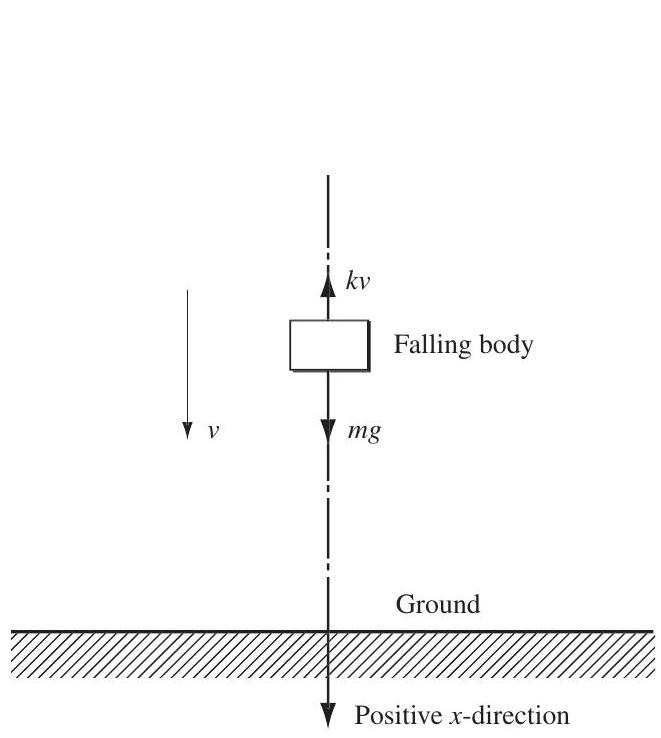
\includegraphics[max width=\textwidth]{2024_04_03_5bb5b4275a64cb9887d1g-069(1)}
\end{center}

Fig. 7-1

\begin{center}
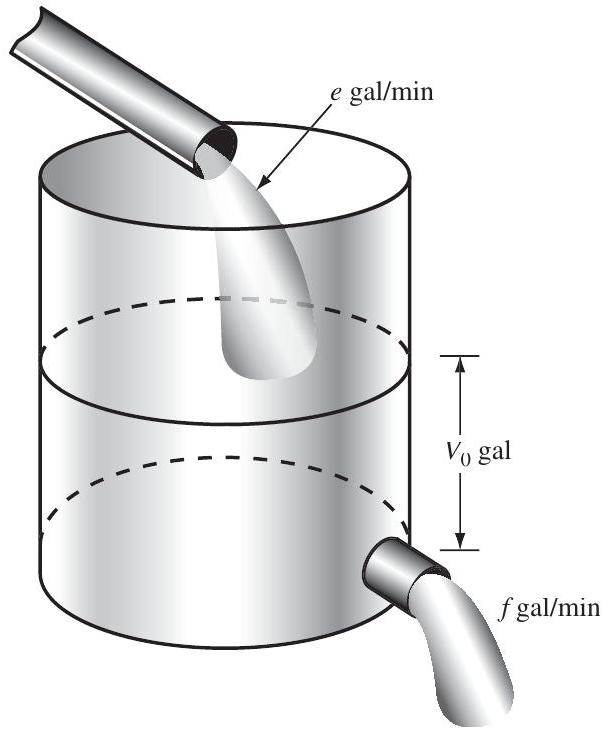
\includegraphics[max width=\textwidth]{2024_04_03_5bb5b4275a64cb9887d1g-069}
\end{center}

Fig. 7-2

(See Problem 7.11.) When $k>0$, the limiting velocity $v_{l}$ is defined by


\begin{equation*}
v_{l}=\frac{m g}{k} \tag{7.6}
\end{equation*}


Caution: Equations (7.4), (7.5), and (7.6), are valid only if the given conditions are satisfied. These equations are not valid if, for example, air resistance is not proportional to velocity but to the velocity squared, or if the upward direction is taken to be the positive direction. (See Problems 7.14 and 7.15.)

\section*{DILUTION PROBLEMS}
Consider a tank which initially holds $V_{0}$ gal of brine that contains $a \mathrm{lb}$ of salt. Another brine solution, containing $b \mathrm{lb}$ of salt per gallon, is poured into the tank at the rate of $e \mathrm{gal} / \mathrm{min}$ while, simultaneously, the well-stirred solution leaves the tank at the rate of $f \mathrm{gal} / \mathrm{min}$ (Fig. 7-2). The problem is to find the amount of salt in the tank at any time $t$.

Let $Q$ denote the amount (in pounds) of salt in the tank at any time $t$. The time rate of change of $Q, d Q / d t$, equals the rate at which salt enters the tank minus the rate at which salt leaves the tank. Salt enters the tank at the rate of $\mathrm{be} \mathrm{lb} / \mathrm{min}$. To determine the rate at which salt leaves the tank, we first calculate the volume of brine in the tank at any time $t$, which is the initial volume $V_{0}$ plus the volume of brine added $e t$ minus the volume of brine removed $f t$. Thus, the volume of brine at any time is


\begin{equation*}
V_{0}+e t-f t \tag{7.7}
\end{equation*}


The concentration of salt in the tank at any time is $Q /\left(V_{0}+e t-f t\right)$, from which it follows that salt leaves the tank at the rate of

Thus,

$$
f\left(\frac{Q}{V_{0}+e t-f t}\right) \mathrm{lb} / \mathrm{min}
$$

$$
\frac{d Q}{d t}=b e-f\left(\frac{Q}{V_{0}+e t-f t}\right)
$$

or


\begin{equation*}
\frac{d Q}{d t}+\frac{f}{V_{0}+(e-f) t} Q=b e \tag{7.8}
\end{equation*}


(See Problems 7.16-7.18.)

\section*{ELECTRICAL CIRCUITS}
The basic equation governing the amount of current $I$ (in amperes) in a simple RL circuit (Fig. 7-3) consisting of a resistance $R$ (in ohms), an inductor $L$ (in henries), and an electromotive force (abbreviated emf) $E$ (in volts) is


\begin{equation*}
\frac{d I}{d t}+\frac{R}{L} I=\frac{E}{L} \tag{7.9}
\end{equation*}


For an RC circuit consisting of a resistance, a capacitance $C$ (in farads), an emf, and no inductance (Fig. 7-4), the equation governing the amount of electrical charge $q$ (in coulombs) on the capacitor is


\begin{equation*}
\frac{d q}{d t}+\frac{1}{R C} q=\frac{E}{R} \tag{7.10}
\end{equation*}


The relationship between $q$ and $I$ is


\begin{equation*}
I=\frac{d q}{d t} \tag{7.11}
\end{equation*}


(See Problems 7.19-7.22.) For more complex circuits see Chapter 14.

\begin{center}
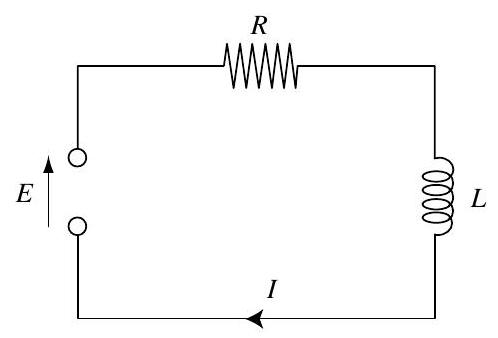
\includegraphics[max width=\textwidth]{2024_04_03_5bb5b4275a64cb9887d1g-071(1)}
\end{center}

Fig. 7-3

\begin{center}
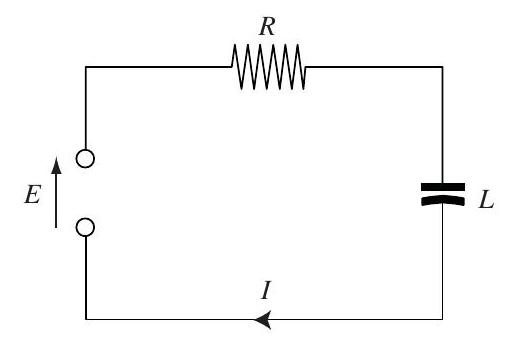
\includegraphics[max width=\textwidth]{2024_04_03_5bb5b4275a64cb9887d1g-071}
\end{center}

Fig. 7-4

\section*{ORTHOGONAL TRAJECTORIES}
Consider a one-parameter family of curves in the $x y$-plane defined by


\begin{equation*}
F(x, y, c)=0 \tag{7.12}
\end{equation*}


where $c$ denotes the parameter. The problem is to find another one-parameter family of curves, called the orthogonal trajectories of the family (7.12) and given analytically by


\begin{equation*}
G(x, y, k)=0 \tag{7.13}
\end{equation*}


such that every curve in this new family (7.13) intersects at right angles every curve in the original family (7.12).

We first implicitly differentiate (7.12) with respect to $x$, then eliminate $c$ between this derived equation and (7.12). This gives an equation connecting $x, y$, and $y^{\prime}$, which we solve for $y^{\prime}$ to obtain a differential equation of the form


\begin{equation*}
\frac{d \dot{y}}{d x}=f(x, y) \tag{7.14}
\end{equation*}


The orthogonal trajectories of (7.12) are the solutions of


\begin{equation*}
\frac{d y}{d x}=-\frac{1}{f(x, y)} \tag{7.15}
\end{equation*}


(See Problems 7.23-7.25.)

For many families of curves, one cannot explicitly solve for $d y / d x$ and obtain a differential equation of the form (7.14). We do not consider such curves in this book.

\section*{Solved Problems}
7.1. A person places $\$ 20,000$ in a savings account which pays 5 percent interest per annum, compounded continuously. Find $(a)$ the amount in the account after three years, and $(b)$ the time required for the account to double in value, presuming no withdrawals and no additional deposits.

Let $N(t)$ denote the balance in the account at any time $t$. Initially, $N(0)=20,000$. The balance in the account grows by the accumulated interest payments, which are proportional to the amount of money in the account. The constant of proportionality is the interest rate. In this case, $k=0.05$ and Eq. (7.1) becomes

$$
\frac{d N}{d t}-0.05 N=0
$$

This differential equation is both linear and separable. Its solution is


\begin{equation*}
N(t)=c e^{0.05 t} \tag{1}
\end{equation*}


At $t=0, N(0)=20,000$, which when substituted into (1) yields

$$
20,000=c e^{0.05(0)}=c
$$

With this value of $c,(1)$ becomes


\begin{equation*}
N(t)=20,000 e^{0.05 t} \tag{2}
\end{equation*}


Equation (2) gives the dollar balance in the account at any time $t$.

(a) Substituting $t=3$ into (2), we find the balance after three years to be

$$
N(3)=20,000 e^{0.05(3)}=20,000(1.161834)=\$ 23,236.68
$$

(b) We seek the time $t$ at which $N(t)=\$ 40,000$. Substituting these values into (2) and solving for $t$, we obtain

$$
\begin{aligned}
40,000 & =20,000 e^{0.05 t} \\
2 & =e^{0.05 t} \\
\ln |2| & =0.05 t \\
t=\frac{1}{0.05} \ln |2| & =13.86 \text { years }
\end{aligned}
$$

7.2. A person places $\$ 5000$ in an account that accrues interest compounded continuously. Assuming no additional deposits or withdrawals, how much will be in the account after seven years if the interest rate is a constant 8.5 percent for the first four years and a constant 9.25 percent for the last three years?

Let $N(t)$ denote the balance in the account at any time $t$. Initially, $N(0)=5000$. For the first four years, $k=0.085$ and Eq. (7.1) becomes

$$
\frac{d N}{d t}-0.085 N=0
$$

Its solution is


\begin{equation*}
N(t)=c e^{0.085 t} \quad(0 \leq t \leq 4) \tag{1}
\end{equation*}


At $t=0, N(0)=5000$, which when substituted into (1) yields

and (1) becomes

$$
5000=c e^{0.085(0)}=c
$$


\begin{equation*}
N(t)=5000 e^{0.085 t} \quad(0 \leq t \leq 4) \tag{2}
\end{equation*}


Substituting $t=4$ into (2), we find the balance after four years to be

$$
N(t)=5000 e^{0.085(4)}=5000(1.404948)=\$ 7024.74
$$

This amount also represents the beginning balance for the last three-year period.

Over the last three years, the interest rate is 9.25 percent and (7.1) becomes

$$
\frac{d N}{d t}-0.0925 N=0 \quad(4 \leq t \leq 7)
$$

Its solution is


\begin{equation*}
N(t)=c e^{0.0925 t} \quad(4 \leq t \leq 7) \tag{3}
\end{equation*}


At $t=4, N(4)=\$ 7024.74$, which when substituted into (3) yields

$$
7024.74=c e^{0.0925(4)}=c(1.447735) \quad \text { or } \quad c=4852.23
$$

and (3) becomes


\begin{equation*}
N(t)=4852.23 e^{0.0925 t} \quad(4 \leq t \leq 7) \tag{4}
\end{equation*}


Substituting $t=7$ into (4), we find the balance after seven years to be

$$
N(7)=4852.23 e^{0.0925(7)}=4852.23(1.910758)=\$ 9271.44
$$

7.3. What constant interest rate is required if an initial deposit placed into an account that accrues interest compounded continuously is to double its value in six years?

The balance $N(t)$ in the account at any time $t$ is governed by (7.1)

$$
\frac{d N}{d t}-k N=0
$$

which has as its solution


\begin{equation*}
N(t)=c e^{k t} \tag{1}
\end{equation*}


We are not given an amount for the initial deposit, so we denote it as $N_{0}$. At $t=0, N(0)=N_{0}$, which when substituted into (1) yields

$$
N_{0}=c e^{k(0)}=c
$$

and (1) becomes


\begin{equation*}
N(t)=N_{0} e^{k t} \tag{2}
\end{equation*}


We seek the value of $k$ for which $N=2 N_{0}$ when $t=6$. Substituting these values into (2) and solving for $k$, we find

$$
\begin{aligned}
2 N_{0} & =N_{0} e^{k(6)} \\
e^{6 k} & =2 \\
6 k & =\ln |2| \\
k=\frac{1}{6} \ln |2| & =0.1155
\end{aligned}
$$

An interest rate of 11.55 percent is required.

7.4. A bacteria culture is known to grow at a rate proportional to the amount present. After one hour, 1000 strands of the bacteria are observed in the culture; and after four hours, 3000 strands. Find (a) an expression for the approximate number of strands of the bacteria present in the culture at any time $t$ and $(b)$ the approximate number of strands of the bacteria originally in the culture.

(a) Let $N(t)$ denote the number of bacteria strands in the culture at time $t$. From $(6.1), d N / d t-k N=0$, which is both linear and separable. Its solution is


\begin{equation*}
N(t)=c e^{k t} \tag{1}
\end{equation*}


At $t=1, N=1000$; hence,


\begin{equation*}
1000=c e^{k} \tag{2}
\end{equation*}


At $t=4, N=3000$; hence,


\begin{equation*}
3000=c e^{4 k} \tag{3}
\end{equation*}


Solving (2) and (3) for $k$ and $c$, we find

$$
k=\frac{1}{3} \ln 3=0.366 \quad \text { and } c=1000 e^{-0.366}=694
$$

Substituting these values of $k$ and $c$ into (1), we obtain


\begin{equation*}
N(t)=694 e^{0.366 t} \tag{4}
\end{equation*}


as an expression for the amount of the bacteria present at any time $t$.

(b) We require $N$ at $t=0$. Substituting $t=0$ into (4), we obtain $N(0)=694 e^{(0.366)(0)}=694$.

7.5. The population of a certain country is known to increase at a rate proportional to the number of people presently living in the country. If after two years the population has doubled, and after three years the population is 20,000 , estimate the number of people initially living in the country.

Let $N$ denote the number of people living in the country at any time $t$, and let $N_{0}$ denote the number of people initially living in the country. Then, from (7.1),

$$
\frac{d N}{d t}-k N=0
$$

which has the solution


\begin{equation*}
N=c e^{k t} \tag{1}
\end{equation*}


At $t=0, N=N_{0}$; hence, it follows from (1) that $N_{0}=c e^{k(0)}$, or that $c=N_{0}$. Thus,


\begin{equation*}
N=N_{0} e^{k t} \tag{2}
\end{equation*}


At $t=2, N=2 N_{0}$. Substituting these values into (2), we have

$$
2 N_{0}=N_{0} e^{2 k} \quad \text { from which } \quad k=\frac{1}{2} \ln 2=0.347
$$

Substituting this value into (2) gives


\begin{equation*}
N=N_{0} e^{0.347 t} \tag{3}
\end{equation*}


At $t=3, N=20,000$. Substituting these values into (3), we obtain

$$
20,000=N_{0} e^{(0.347)(3)}=N_{0}(2.832) \quad \text { or } \quad N_{0}=7062
$$

7.6. A certain radioactive material is known to decay at a rate proportional to the amount present. If initially there is 50 milligrams of the material present and after two hours it is observed that the material has lost 10 percent of its original mass, find (a) an expression for the mass of the material remaining at any time $t$, (b) the mass of the material after four hours, and (c) the time at which the material has decayed to one half of its initial mass.

(a) Let $N$ denote the amount of material present at time $t$. Then, from (7.1),

$$
\frac{d N}{d t}-k N=0
$$

This differential equation is separable and linear; its solution is


\begin{equation*}
N=c e^{k t} \tag{1}
\end{equation*}


At $t=0$, we are given that $N=50$. Therefore, from (1), $50=c e^{k(0)}$, or $c=50$. Thus,


\begin{equation*}
N=50 e^{k t} \tag{2}
\end{equation*}


At $t=2,10$ percent of the original mass of $50 \mathrm{mg}$, or $5 \mathrm{mg}$, has decayed. Hence, at $t=2, N=50-5=45$. Substituting these values into (2) and solving for $k$, we have

$$
45=50 e^{2 k} \quad \text { or } \quad k=\frac{1}{2} \ln \frac{45}{50}=-0.053
$$

Substituting this value into (2), we obtain the amount of mass present at any time $t$ as

where $t$ is measured in hours.


\begin{equation*}
N=50 e^{-0.053 t} \tag{3}
\end{equation*}


(b) We require $N$ at $t=4$. Substituting $t=4$ into (3) and then solving for $N$, we find that

$$
N=50 e^{(-0.053)(4)}=50(0.809)=40.5 \mathrm{mg}
$$

(c) We require $t$ when $N=50 / 2=25$. Substituting $N=25$ into (3) and solving for $t$, we find

$$
25=50 e^{-0.053 t} \quad \text { or } \quad-0.053 t=\ln \frac{1}{2} \quad \text { or } \quad t=13 \text { hours }
$$

The time required to reduce a decaying material to one half its original mass is called the half-life of the material. For this problem, the half-life is 13 hours.

7.7. Five mice in a stable population of 500 are intentionally infected with a contagious disease to test a theory of epidemic spread that postulates the rate of change in the infected population is proportional to the product of the number of mice who have the disease with the number that are disease free. Assuming the theory is correct, how long will it take half the population to contract the disease?

Let $N(t)$ denote the number of mice with the disease at time $t$. We are given that $N(0)=5$, and it follows that $500-N(t)$ is the number of mice without the disease at time $t$. The theory predicts that


\begin{equation*}
\frac{d N}{d t}=k N(500-N) \tag{1}
\end{equation*}


where $k$ is a constant of proportionality. This equation is different from (7.1) because the rate of change is no longer proportional to just the number of mice who have the disease. Equation (1) has the differential form


\begin{equation*}
\frac{d N}{N(500-N)}-k d t=0 \tag{2}
\end{equation*}


which is separable. Using partial fraction decomposition, we have

$$
\frac{1}{N(500-N)}=\frac{1 / 500}{N}+\frac{1 / 500}{500-N}
$$

hence (2) may be rewritten as

$$
\frac{1}{500}\left(\frac{1}{N}+\frac{1}{500-N}\right) d N-k d t=0
$$

Its solution is

or

$$
\begin{aligned}
& \frac{1}{500} \int\left(\frac{1}{N}+\frac{1}{500-N}\right) d N-\int k d t=c \\
& \frac{1}{500}(\ln |N|-\ln |500-N|)-k t=c
\end{aligned}
$$

which may be rewritten as


\begin{align*}
\ln \left|\frac{N}{500-N}\right| & =500(c+k t) \\
\frac{N}{500-N} & =e^{500(c+k t)} \tag{3}
\end{align*}


But $e^{500(c+k t)}=e^{500 c} e^{500 k t}$. Setting $c_{1}=e^{500 c}$, we can write (3) as


\begin{equation*}
\frac{N}{500-N}=c_{1} e^{500 k t} \tag{4}
\end{equation*}


At $t=0, N=5$. Substituting these values into (4), we find

$$
\frac{5}{495}=c_{1} e^{500 k(0)}=c_{1}
$$

so $c_{1}=1 / 99$ and (4) becomes


\begin{equation*}
\frac{N}{500-N}=\frac{1}{99} e^{500 k t} \tag{5}
\end{equation*}


We could solve (5) for $N$, but this is not necessary. We seek a value of $t$ when $N=250$, one-half the population. Substituting $N=250$ into (5) and solving for $t$, we obtain

$$
\begin{aligned}
1 & =\frac{1}{99} e^{500 k t} \\
99 & =e^{500 k t} \\
\ln 99 & =500 k t
\end{aligned}
$$

or $t=0.00919 / k$ time units. Without additional information, we cannot obtain a numerical value for the constant of proportionality $k$ or be more definitive about $t$.

7.8. A metal bar at a temperature of $100^{\circ} \mathrm{F}$ is placed in a room at a constant temperature of $0^{\circ} \mathrm{F}$. If after 20 minutes the temperature of the bar is $50^{\circ} \mathrm{F}$, find $(a)$ the time it will take the bar to reach a temperature of $25^{\circ} \mathrm{F}$ and $(b)$ the temperature of the bar after 10 minutes.

Use Eq. (7.2) with $T_{m}=0$; the medium here is the room which is being held at a constant temperature of $0^{\circ} \mathrm{F}$. Thus we have

$$
\frac{d T}{d t}+k T=0
$$

whose solution is


\begin{equation*}
T=c e^{-k t} \tag{1}
\end{equation*}


Since $T=100$ at $t=0$ (the temperature of the bar is initially $100^{\circ} \mathrm{F}$ ), it follows from (1) that $100=c e^{-k(0)}$ or $100=c$. Substituting this value into (1), we obtain


\begin{equation*}
T=100 e^{-k t} \tag{2}
\end{equation*}


At $t=20$, we are given that $T=50$; hence, from (2),

$$
50=100 e^{-20 k} \quad \text { from which } \quad k=\frac{-1}{20} \ln \frac{50}{100}=\frac{-1}{20}(-0.693)=0.035
$$

Substituting this value into (2), we obtain the temperature of the bar at any time $t$ as


\begin{equation*}
T=100 e^{-0.035 t} \tag{3}
\end{equation*}


(a) We require $t$ when $T=25$. Substituting $T=25$ into (3), we have

$$
25=100 e^{-0.035 t} \quad \text { or } \quad-0.035 t=\ln \frac{1}{4}
$$

Solving, we find that $t=39.6 \mathrm{~min}$.

(b) We require $T$ when $t=10$. Substituting $t=10$ into (3) and then solving for $T$, we find that

$$
T=100 e^{(-0.035)(10)}=100(0.705)=70.5^{\circ} \mathrm{F}
$$

It should be noted that since Newton's law is valid only for small temperature differences, the above calculations represent only a first approximation to the physical situation.

7.9. A body at a temperature of $50^{\circ} \mathrm{F}$ is placed outdoors where the temperature is $100^{\circ} \mathrm{F}$. If after 5 minutes the temperature of the body is $60^{\circ} \mathrm{F}$, find $(a)$ how long it will take the body to reach a temperature of $75^{\circ} \mathrm{F}$ and $(b)$ the temperature of the body after 20 minutes.

Using (7.2) with $T_{m}=100$ (the surrounding medium is the outside air), we have

$$
\frac{d T}{d t}+k T=100 k
$$

This differential equation is linear. Its solution is given in Problem 6.15 as


\begin{equation*}
T=c e^{-k t}+100 \tag{1}
\end{equation*}


Since $T=50$ when $t=0$, it follows from (1) that $50=c e^{-k(0)}+100$, or $c=-50$. Substituting this value into (1), we obtain


\begin{equation*}
T=-50 e^{-k t}+100 \tag{2}
\end{equation*}


At $t=5$, we are given that $T=60$; hence, from (2), $60=-50 e^{-5 k}+100$. Solving for $k$, we obtain

$$
-40=-50 e^{-5 k} \quad \text { or } \quad k=\frac{-1}{5} \ln \frac{40}{50}=\frac{-1}{5}(-0.223)=0.045
$$

Substituting this value into (2), we obtain the temperature of the body at any time $t$ as


\begin{equation*}
T=-50 e^{-0.045 t}+100 \tag{3}
\end{equation*}


(a) We require $t$ when $T=75$. Substituting $T=75$ into (3), we have

$$
75=-50 e^{-0.045 t}+100 \text { or } e^{-0.045 t}=\frac{1}{2}
$$

Solving for $t$, we find

$$
-0.045 t=\ln \frac{1}{2} \quad \text { or } \quad t=15.4 \mathrm{~min}
$$

(b) We require $T$ when $t=20$. Substituting $t=20$ into (3) and then solving for $T$, we find

$$
T=-50 e^{(-0.045)(20)}+100=-50(0.41)+100=79.5^{\circ} \mathrm{F}
$$

7.10. A body at an unknown temperature is placed in a room which is held at a constant temperature of $30^{\circ} \mathrm{F}$. If after 10 minutes the temperature of the body is $0^{\circ} \mathrm{F}$ and after 20 minutes the temperature of the body is $15^{\circ} \mathrm{F}$, find the unknown initial temperature.

From (7.2),

$$
\frac{d T}{d t}+k T=30 k
$$

Solving, we obtain


\begin{equation*}
T=c e^{-k t}+30 \tag{1}
\end{equation*}


At $t=10$, we are given that $T=0$. Hence, from (1),


\begin{equation*}
0=c e^{-10 k}+30 \quad \text { or } \quad c e^{-10 k}=-30 \tag{2}
\end{equation*}


At $t=20$, we are given that $T=15$. Hence, from (1) again,


\begin{equation*}
15=c e^{-20 k}+30 \quad \text { or } \quad c e^{-20 k}=-15 \tag{3}
\end{equation*}


Solving (2) and (3) for $k$ and $c$, we find

$$
k=\frac{1}{10} \ln 2=0.069 \quad \text { and } \quad c=-30 e^{10 k}=-30(2)=-60
$$

Substituting these values into (1), we have for the temperature of the body at any time $t$


\begin{equation*}
T=-60 e^{-0.069 t}+30 \tag{4}
\end{equation*}


Since we require $T$ at the initial time $t=0$, it follows from (4) that

$$
T_{0}=-60 e^{(-0.069)(0)}+30=-60+30=-30^{\circ} \mathrm{F}
$$

7.11. A body of mass 5 slugs is dropped from a height of $100 \mathrm{ft}$ with zero velocity. Assuming no air resistance, find $(a)$ an expression for the velocity of the body at any time $t,(b)$ an expression for the position of the body at any time $t$, and $(c)$ the time required to reach the ground.

\begin{center}
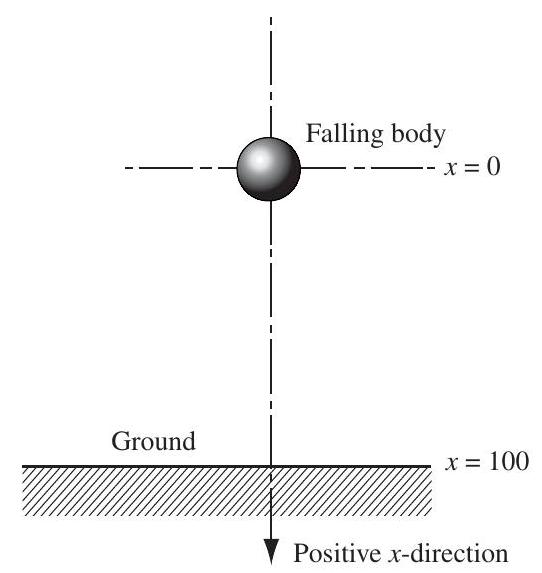
\includegraphics[max width=\textwidth]{2024_04_03_5bb5b4275a64cb9887d1g-078}
\end{center}

Fig. 7-5

(a) Choose the coordinate system as in Fig. 7-5. Then, since there is no air resistance, (7.5) applies: $d v / d t=g$. This differential equation is linear or, in differential form, separable; its solution is $v=g t+c$. When $t=0, v=0$ (initially the body has zero velocity); hence $0=g(0)+c$, or $c=0$. Thus, $v=g t$ or, assuming $g=32 \mathrm{ft} / \mathrm{sec}^{2}$,


\begin{equation*}
v=32 t \tag{1}
\end{equation*}


(b) Recall that velocity is the time rate of change of displacement, designated here by $x$. Hence, $v=d x / d t$, and (1) becomes $d x / d t=32 t$. This differential equation is also both linear and separable; its solution is


\begin{equation*}
x=16 t^{2}+c_{1} \tag{2}
\end{equation*}


But at $t=0, x=0$ (see Fig. 7-5). Thus, $0=(16)(0)^{2}+c_{1}$, or $c_{1}=0$. Substituting this value into (2), we have


\begin{equation*}
x=16 t^{2} \tag{3}
\end{equation*}


(c) We require $t$ when $x=100$. From (3) $t=\sqrt{(100) /(16)}=2.5 \mathrm{sec}$.

7.12. A steel ball weighing $2 \mathrm{lb}$ is dropped from a height of $3000 \mathrm{ft}$ with no velocity. As it falls, the ball encounters air resistance numerically equal to $v / 8$ (in pounds), where $v$ denotes the velocity of the ball (in feet per second). Find $(a)$ the limiting velocity for the ball and $(b)$ the time required for the ball to hit the ground.

Locate the coordinate system as in Fig. 7-5 with the ground now situated at $x=3000$. Here $w=2 \mathrm{lb}$ and $k=1 / 8$. Assuming gravity $g$ is $32 \mathrm{ft} / \mathrm{sec}^{2}$, we have from the formula $w=m g$ that $2=m(32)$ or that the mass of the ball is $m=1 / 16$ slug. Equation (7.4) becomes

$$
\frac{d v}{d t}+2 v=32
$$

which has as its solution


\begin{equation*}
v(t)=c e^{-2 t}+16 \tag{1}
\end{equation*}


At $t=0$, we are given that $v=0$. Substituting these values into (1), we obtain

$$
0=c e^{-2(0)}+16=c+16
$$

from which we conclude that $c=-16$ and (1) becomes


\begin{equation*}
v(t)=-16 e^{-2 t}+16 \tag{2}
\end{equation*}


(a) From (1) or (2), we see that as $t \rightarrow \infty, v \rightarrow 16$ so the limiting velocity is $16 \mathrm{ft} / \mathrm{sec}^{2}$.

(b) To find the time it takes for the ball to hit the ground $(x=3000)$, we need an expression for the position of the ball at any time $t$. Since $v=d x / d t$, (2) can be rewritten as

$$
\frac{d x}{d t}=-16 e^{-2 t}+16
$$

Integrating both sides of this last equation directly with respect to $t$, we have


\begin{equation*}
x(t)=8 e^{-2 t}+16 t+c_{1} \tag{3}
\end{equation*}


where $c_{1}$ denotes a constant of integration. At $t=0, x=0$. Substituting these values into (3), we obtain

$$
0=8 e^{-2(0)}+16(0)+c_{1}=8+c_{1}
$$

from which we conclude that $c_{1}=-8$ and (3) becomes


\begin{equation*}
x(t)=8 e^{-2 t}+16 t-8 \tag{4}
\end{equation*}


The ball hits the ground when $x(t)=3000$. Substituting this value into (4), we have

or


\begin{gather*}
3000=8 e^{-2 t}+16 t-8 \\
376=e^{-2 t}+2 t \tag{5}
\end{gather*}


Although (5) cannot be solved explicitly for $t$, we can approximate the solution by trial and error, substituting different values of $t$ into (5) until we locate a solution to the degree of accuracy we need. Alternatively, we note that for any large value of $t$, the negative exponential term will be negligible. A good approximation is obtained by setting $2 t=376$ or $t=188 \mathrm{sec}$. For this value of $t$, the exponential is essentially zero.

7.13. A body weighing $64 \mathrm{lb}$ is dropped from a height of $100 \mathrm{ft}$ with an initial velocity of $10 \mathrm{ft} / \mathrm{sec}$. Assume that the air resistance is proportional to the velocity of the body. If the limiting velocity is known to be $128 \mathrm{ft} / \mathrm{sec}$, find ( $a$ ) an expression for the velocity of the body at any time $t$ and $(b)$ an expression for the position of the body at any time $t$.

(a) Locate the coordinate system as in Fig. 7-5. Here $w=64 \mathrm{lb}$. Since $w=m g$, it follows that $m g=64$, or $m=2$ slugs. Given that $v_{1}=128 \mathrm{ft} / \mathrm{sec}$, it follows from (7.6) that $128=64 / k$, or $k=\frac{1}{2}$. Substituting these values into (6.4), we obtain the linear differential equation

$$
\frac{d v}{d t}+\frac{1}{4} v=32
$$

which has the solution


\begin{equation*}
v=c e^{-t / 4}+128 \tag{1}
\end{equation*}


At $t=0$, we are given that $v=10$. Substituting these values into (1), we have $10=c e^{0}+128$, or $c=-118$. The velocity at any time $t$ is given by


\begin{equation*}
v=-118 e^{-t / 4}+128 \tag{2}
\end{equation*}


(b) Since $v=d x / d t$, where $x$ is displacement, (2) can be rewritten as

$$
\frac{d x}{d t}=-118 e^{-t / 4}+128
$$

This last equation, in differential form, is separable; its solution is


\begin{equation*}
x=472 e^{-t / 4}+128 t+c_{1} \tag{3}
\end{equation*}


At $t=0$, we have $x=0$ (see Fig. 7-5). Thus, (3) gives

$$
0=472 e^{0}+(128)(0)+c_{1} \quad \text { or } \quad c_{1}=-472
$$

The displacement at any time $t$ is then given by

$$
x=472 e^{-t / 4}+128 t-472
$$

7.14. A body of mass $m$ is thrown vertically into the air with an initial velocity $v_{0}$. If the body encounters an air resistance proportional to its velocity, find $(a)$ the equation of motion in the coordinate system of Fig. 7-6, (b) an expression for the velocity of the body at any time $t$, and $(c)$ the time at which the body reaches its maximum height.

\begin{center}
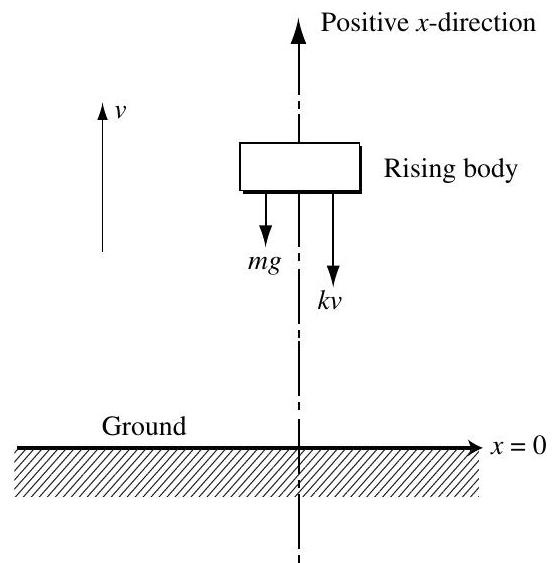
\includegraphics[max width=\textwidth]{2024_04_03_5bb5b4275a64cb9887d1g-080}
\end{center}

Fig. 7-6

(a) In this coordinate system, Eq. (7.4) may not be the equation of motion. To derive the appropriate equation, we note that there are two forces on the body: (1) the force due to the gravity given by $m g$ and (2) the force due to air resistance given by $k v$, which will impede the velocity of the body. Since both of these forces act in the downward or negative direction, the net force on the body is $-m g-k v$. Using (7.3) and rearranging, we obtain


\begin{equation*}
\frac{d v}{d t}+\frac{k}{m} v=-g \tag{1}
\end{equation*}


as the equation of motion.

(b) Equation (1) is a linear differential equation, and its solution is $v=c e^{-(k / m) t}-m g / k$. At $t=0, v=v_{0}$; hence $v_{0}=c e^{-(k / m) 0}-(m g / k)$, or $c=v_{0}+(m g / k)$. The velocity of the body at any time $t$ is


\begin{equation*}
v=\left(v_{0}+\frac{m g}{k}\right) e^{-(k / m) t}-\frac{m g}{k} \tag{2}
\end{equation*}


(c) The body reaches its maximum height when $v=0$. Thus, we require $t$ when $v=0$. Substituting $v=0$ into (2) and solving for $t$, we find

$$
\begin{aligned}
0 & =\left(v_{0}+\frac{m g}{k}\right) e^{-(k / m) t}-\frac{m g}{k} \\
e^{-(k / m) t} & =\frac{1}{1+\frac{v_{0} k}{m g}} \\
-(k / m) t & =\ln \left(\frac{1}{1+\frac{v_{0} k}{m g}}\right) \\
t & =\frac{m}{k} \ln \left(1+\frac{v_{0} k}{m g}\right)
\end{aligned}
$$

7.15. A body of mass 2 slugs is dropped with no initial velocity and encounters an air resistance that is proportional to the square of its velocity. Find an expression for the velocity of the body at any time $t$.

The force due to air resistance is $-k v^{2}$; so that Newton's second law of motion becomes

$$
m \frac{d v}{d t}=m g-k v^{2} \quad \text { or } \quad 2 \frac{d v}{d t}=64-k v^{2}
$$

Rewriting this equation in differential form, we have


\begin{equation*}
\frac{2}{64-k v^{2}} d v-d t=0 \tag{1}
\end{equation*}


which is separable. By partial fractions,

$$
\frac{2}{64-k v^{2}}=\frac{2}{(8-\sqrt{k} v)(8+\sqrt{k} v)}=\frac{\frac{1}{8}}{8-\sqrt{k} v}+\frac{\frac{1}{8}}{8+\sqrt{k} v}
$$

Hence (1) can be rewritten as

$$
\frac{1}{8}\left(\frac{1}{8-\sqrt{k} v}+\frac{1}{8+\sqrt{k} v}\right) d v-d t=0
$$

This last equation has as its solution

or

$$
\begin{gathered}
\frac{1}{8} \int\left(\frac{1}{8-\sqrt{k} v}+\frac{1}{8+\sqrt{k} v}\right) d v-\int d t=c \\
\frac{1}{8}\left[-\frac{1}{\sqrt{k}} \ln |8-\sqrt{k} v|+\frac{1}{\sqrt{k}} \ln |8+\sqrt{k} v|\right]-t=c
\end{gathered}
$$

which can be rewritten as

or

$$
\begin{gathered}
\ln \left|\frac{8+\sqrt{k} v}{8-\sqrt{k} v}\right|=8 \sqrt{k} t+8 \sqrt{k} c \\
\frac{8+\sqrt{k} v}{8-\sqrt{k} v}=c_{1} e^{8 \sqrt{k} t} \quad\left(c_{1}= \pm e^{8 \sqrt{k} c}\right)
\end{gathered}
$$

At $t=0$, we are given that $v=0$. This implies $c_{1}=1$, and the velocity is given by

$$
\frac{8+\sqrt{k} v}{8-\sqrt{k} v}=e^{8 \sqrt{k} t} \quad \text { or } \quad v=\frac{8}{\sqrt{k}} \tanh 4 \sqrt{k} t
$$

Note that without additional information, we cannot obtain a numerical value for the constant $k$.

7.16. A tank initially holds $100 \mathrm{gal}$ of a brine solution containing $20 \mathrm{lb}$ of salt. At $t=0$, fresh water is poured into the tank at the rate of $5 \mathrm{gal} / \mathrm{min}$, while the well-stirred mixture leaves the tank at the same rate. Find the amount of salt in the tank at any time $t$.

Here, $V_{0}=100, a=20, b=0$, and $e=f=5$. Equation (7.8) becomes

$$
\frac{d Q}{d t}+\frac{1}{20} Q=0
$$

The solution of this linear equation is


\begin{equation*}
Q=c e^{-t / 20} \tag{1}
\end{equation*}


At $t=0$, we are given that $Q=a=20$. Substituting these values into (1), we find that $c=20$, so that (1) can be rewritten as $Q=20 e^{-t / 20}$. Note that as $t \rightarrow \infty, Q \rightarrow 0$ as it should, since only fresh water is being added.

7.17. A tank initially holds $100 \mathrm{gal}$ of a brine solution containing $1 \mathrm{lb}$ of salt. At $t=0$ another brine solution containing $1 \mathrm{lb}$ of salt per gallon is poured into the tank at the rate of $3 \mathrm{gal} / \mathrm{min}$, while the well-stirred mixture leaves the tank at the same rate. Find (a) the amount of salt in the tank at any time $t$ and $(b)$ the time at which the mixture in the tank contains $2 \mathrm{lb}$ of salt.

(a) Here $V_{0}=100, a=1, b=1$, and $e=f=3$; hence, (7.8) becomes

$$
\frac{d Q}{d t}+0.03 Q=3
$$

The solution to this linear differential equation is


\begin{equation*}
Q=c e^{-0.03 t}+100 \tag{1}
\end{equation*}


At $t=0, Q=a=1$. Substituting these values into (1), we find $1=c e^{0}+100$, or $c=-99$. Then (1) can be rewritten as


\begin{equation*}
Q=-99 e^{-0.03 t}+100 \tag{2}
\end{equation*}


(b) We require $t$ when $Q=2$. Substituting $Q=2$ into (2), we obtain

$$
2=-99 e^{-0.03 t}+100 \text { or } e^{-0.03 t}=\frac{98}{99}
$$

from which

$$
t=-\frac{1}{0.03} \ln \frac{98}{99}=0.338 \mathrm{~min}
$$

7.18. A 50-gal tank initially contains $10 \mathrm{gal}$ of fresh water. At $t=0$, a brine solution containing $1 \mathrm{lb}$ of salt per gallon is poured into the tank at the rate of $4 \mathrm{gal} / \mathrm{min}$, while the well-stirred mixture leaves the tank at the rate of $2 \mathrm{gal} / \mathrm{min}$. Find (a) the amount of time required for overflow to occur and (b) the amount of salt in the tank at the moment of overflow.

(a) Here $a=0, b=1, e=4, f=2$, and $V_{0}=10$. The volume of brine in the tank at any time $t$ is given by (7.7) as $V_{0}+e t-f t=10+2 t$. We require $t$ when $10+2 t=50$; hence, $t=20 \mathrm{~min}$.

(b) For this problem, (7.8) becomes

$$
\frac{d Q}{d t}+\frac{2}{10+2 t} Q=4
$$

This is a linear equation; its solution is given in Problem 6.13 as


\begin{equation*}
Q=\frac{40 t+4 t^{2}+c}{10+2 t} \tag{1}
\end{equation*}


At $t=0, Q=a=0$. Substituting these values into (1), we find that $c=0$. We require $Q$ at the moment of\\
overflow, which from part $(a)$ is $t=20$. Thus,

$$
Q=\frac{40(20)+4(20)^{2}}{10+2(20)}=48 \mathrm{lb}
$$

7.19. An RL circuit has an emf of 5 volts, a resistance of $50 \mathrm{ohms}$, an inductance of 1 henry, and no initial current. Find the current in the circuit at any time $t$.

Here $E=5, R=50$, and $L=1$; hence (7.9) becomes

$$
\frac{d I}{d t}+50 I=5
$$

This equation is linear; its solution is

$$
I=c e^{-50 t}+\frac{1}{10}
$$

At $t=0, I=0$; thus, $0=c e^{-50(0)}+\frac{1}{10}$, or $c=-\frac{1}{10}$. The current at any time $t$ is then


\begin{equation*}
I=-\frac{I}{10} e^{-50 t}+\frac{1}{10} \tag{1}
\end{equation*}


The quantity $-\frac{1}{10} e^{-50 t}$ in (1) is called the transient current, since this quantity goes to zero ("dies out") as $t \rightarrow \infty$. The quantity $\frac{1}{10}$ in (1) is called the steady-state current. As $t \rightarrow \infty$, the current $I$ approaches the value of the steadystate current.

7.20. An RL circuit has an emf given (in volts) by $3 \sin 2 t$, a resistance of $10 \mathrm{ohms}$, an inductance of 0.5 henry, and an initial current of 6 amperes. Find the current in the circuit at any time $t$.

Here, $E=3 \sin 2 t, R=10$, and $L=0.5$; hence (7.9) becomes

$$
\frac{d I}{d t}+20 I=6 \sin 2 t
$$

This equation is linear, with solution (see Chapter 6)

$$
\int d\left(I e^{20 t}\right)=\int 6 e^{20 t} \sin 2 t d t
$$

Carrying out the integrations (the second integral requires two integrations by parts), we obtain

$$
I=c e^{-20 t}+\frac{30}{101} \sin 2 t-\frac{3}{101} \cos 2 t
$$

At $t=0, I=6$; hence,

$$
6=c e^{-20(0)}+\frac{30}{101} \sin 2(0)-\frac{3}{101} \cos 2(0) \quad \text { or } \quad 6=c-\frac{3}{101}
$$

whence $c=609 / 101$. The current at any time $t$ is

$$
I=\frac{609}{101} e^{-20 t}+\frac{30}{101} \sin 2 t-\frac{3}{101} \cos 2 t
$$

As in Problem 7.18, the current is the sum of a transient current, here $(609 / 101) e^{-20 t}$, and a steady-state current,

$$
\frac{30}{101} \sin 2 t-\frac{3}{101} \cos 2 t
$$

7.21. Rewrite the steady-state current of Problem 7.20 in the form $A \sin (2 t-\phi)$. The angle $\phi$ is called the phase angle.

Since $A \sin (2 t-\phi)=A(\sin 2 t \cos \phi-\cos 2 t \sin \phi)$, we require

$$
I_{s}=\frac{30}{101} \sin 2 t-\frac{3}{101} \cos 2 t=A \cos \phi \sin 2 t-A \sin \phi \cos 2 t
$$

Thus, $A \cos \phi=\frac{30}{101}$ and $A \sin \phi=\frac{3}{101}$. It now follows that

and

$$
\begin{gathered}
\left(\frac{30}{101}\right)^{2}+\left(\frac{3}{101}\right)^{2}=A^{2} \cos ^{2} \phi+A^{2} \sin ^{2} \phi=A^{2}\left(\cos ^{2} \phi+\sin ^{2} \phi\right)=A^{2} \\
\tan \phi=\frac{A \sin \phi}{A \cos \phi}=\left(\frac{3}{101}\right) /\left(\frac{30}{101}\right)=\frac{1}{10}
\end{gathered}
$$

Consequently, $I_{s}$ has the required form if

$$
A=\sqrt{\frac{909}{(101)^{2}}}=\frac{3}{\sqrt{101}} \text { and } \phi=\arctan \frac{1}{10}=0.0997 \text { radians }
$$

7.22. An $\mathrm{RC}$ circuit has an emf given (in volts) by $400 \cos 2 t$, a resistance of $100 \mathrm{ohms}$, and a capacitance of $10^{-2}$ farad. Initially there is no charge on the capacitor. Find the current in the circuit at any time $t$.

We first find the charge $q$ and then use (7.11) to obtain the current. Here, $E=400 \cos 2 t, R=100$, and $C=10^{-2}$; hence (7.10) becomes

$$
\frac{d q}{d t}+q=4 \cos 2 t
$$

This equation is linear, and its solution is (two integrations by parts are required)

$$
q=c e^{-t}+\frac{8}{5} \sin 2 t+\frac{4}{5} \cos 2 t
$$

At $t=0, q=0$; hence,

Thus

$$
\begin{gathered}
0=c e^{-(0)}+\frac{8}{5} \sin 2(0)+\frac{4}{5} \cos 2(0) \quad \text { or } \quad c=-\frac{4}{5} \\
q=-\frac{4}{5} e^{-t}+\frac{8}{5} \sin 2 t+\frac{4}{5} \cos 2 t
\end{gathered}
$$

and using (7.11), we obtain

$$
I=\frac{d q}{d t}=\frac{4}{5} e^{-t}+\frac{16}{5} \cos 2 t-\frac{8}{5} \sin 2 t
$$

7.23. Find the orthogonal trajectories of the family of curves $x^{2}+y^{2}=c^{2}$.

The family, which is given by (7.12) with $F(x, y, c)=x^{2}+y^{2}-c^{2}$, consists of circles with centers at the origin and radii $c$. Implicitly differentiating the given equation with respect to $x$, we obtain

$$
2 x+2 y y^{\prime}=0 \quad \text { or } \quad \frac{d y}{d x}=-\frac{x}{y}
$$

Here $f(x, y)=-x / y$, so that $(7.15)$ becomes

$$
\frac{d y}{d x}=\frac{y}{x}
$$

This equation is linear (and, in differential form, separable); its solution is


\begin{equation*}
y=k x \tag{1}
\end{equation*}


which represents the orthogonal trajectories.

In Fig. 7-7 some members of the family of circles are shown in solid lines and some members of the family (1), which are straight lines through the origin, are shown in dashed lines. Observe that each straight line intersects each circle at right angles.

\begin{center}
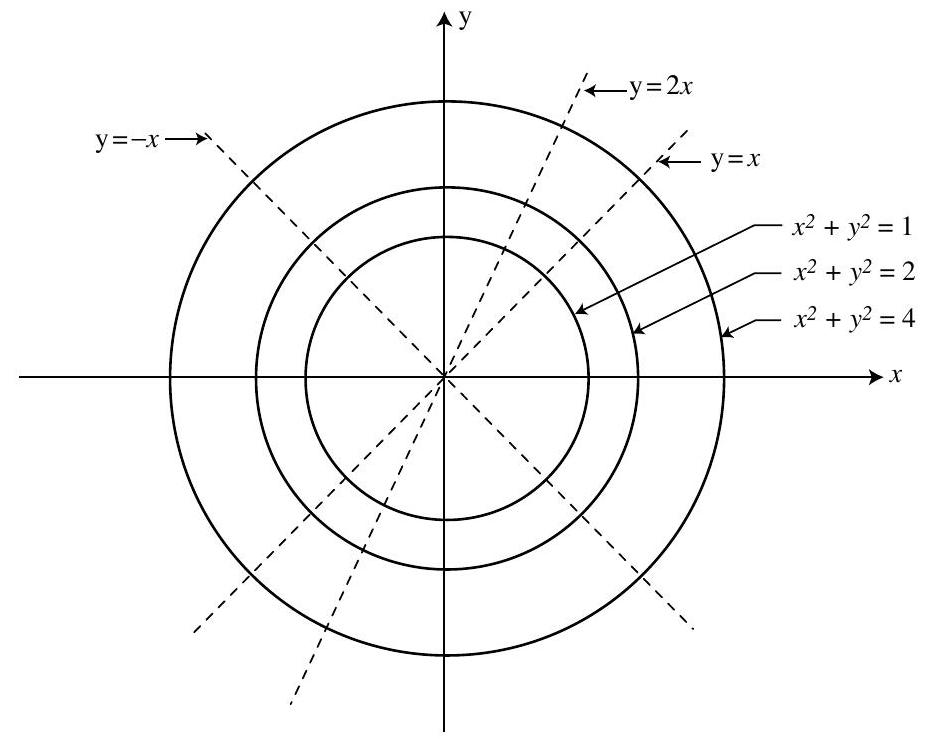
\includegraphics[max width=\textwidth]{2024_04_03_5bb5b4275a64cb9887d1g-085}
\end{center}

Fig. 7-7

7.24. Find the orthogonal trajectories of the family of curves $y=c x^{2}$.

The family, which is given by (7.12) with $F(x, y, c)=y-c x^{2}$, consists of parabolas symmetric about the $y$-axis with vertices at the origin. Differentiating the given equation with respect to $x$, we obtain $d y / d x=2 c x$. To eliminate $c$, we observe, from the given equation, that $c=y / x^{2}$; hence, $d y / d x=2 y / x$. Here $f(x, y)=2 y / x$, so (7.15) becomes

$$
\frac{d y}{d x}=\frac{-x}{2 y} \quad \text { or } \quad x d x+2 y d y=0
$$

The solution of this separable equation is $\frac{1}{2} x^{2}+y^{2}=k$. These orthogonal trajectories are ellipses. Some members of this family, along with some members of the original family of parabolas, are shown in Fig. 7-8. Note that each ellipse intersects each parabola at right angles.

7.25. Find the orthogonal trajectories of the family of curves $x^{2}+y^{2}=c x$.

Here, $F(x, y, c)=x^{2}+y^{2}-c x$. Implicitly differentiating the given equation with respect to $x$, we obtain

$$
2 x+2 y \frac{d y}{d x}=c
$$

\begin{center}
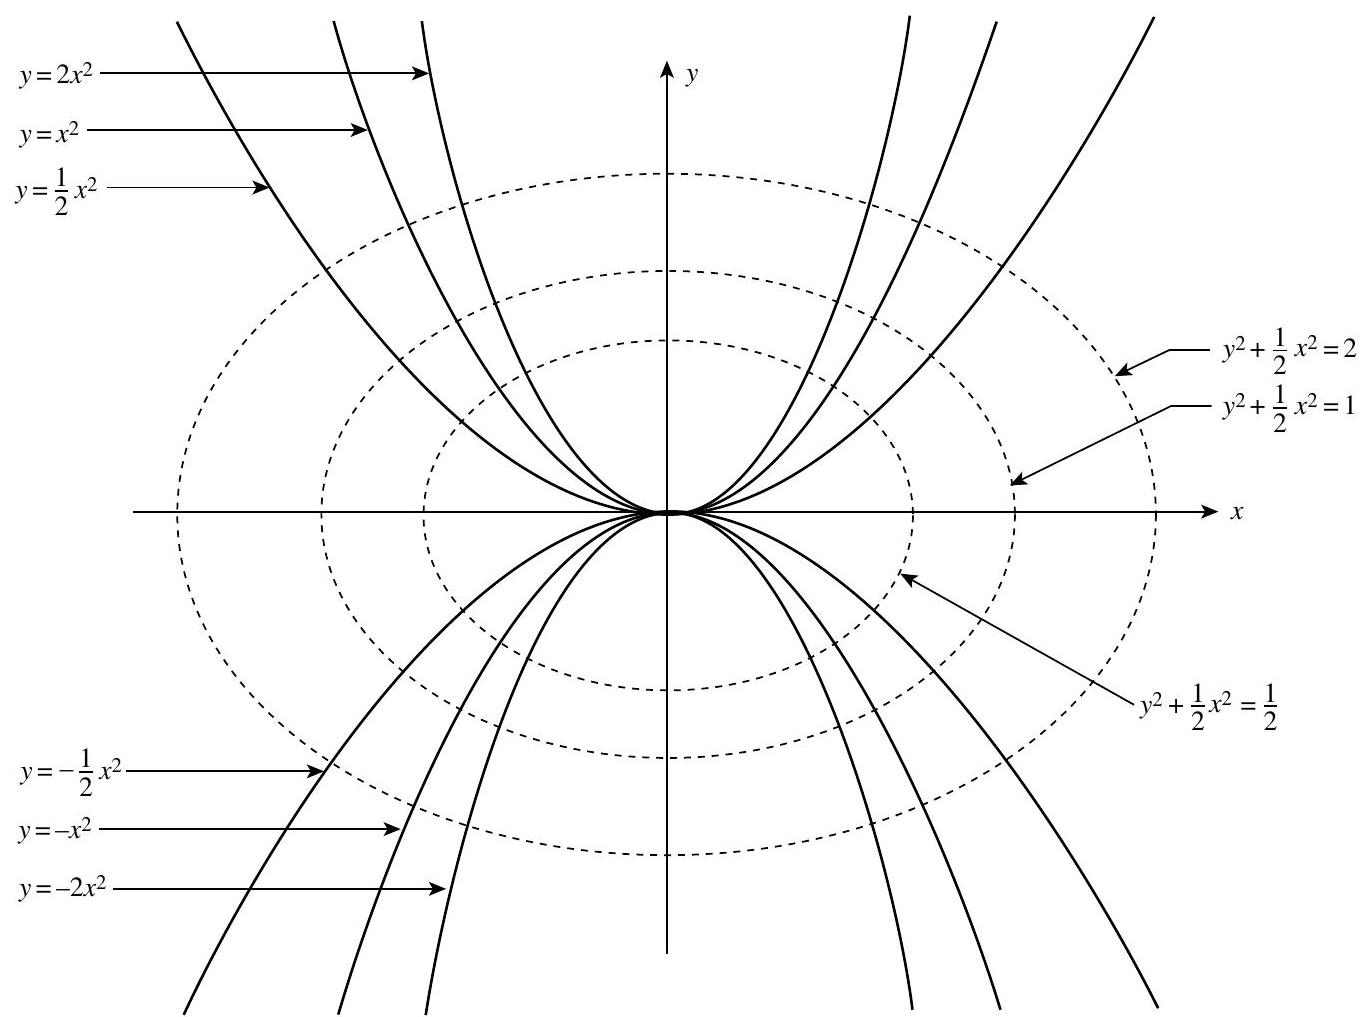
\includegraphics[max width=\textwidth]{2024_04_03_5bb5b4275a64cb9887d1g-086}
\end{center}

Fig. 7-8

Eliminating $c$ between this equation and $x^{2}+y^{2}-c x=0$, we find

$$
2 x+2 y \frac{d y}{d x}=\frac{x^{2}+y^{2}}{x} \text { or } \quad \frac{d y}{d x}=\frac{y^{2}-x^{2}}{2 x y}
$$

Here $f(x, y)=\left(y^{2}-x^{2}\right) / 2 x y$, so $(7.15)$ becomes

$$
\frac{d y}{d x}=\frac{2 x y}{x^{2}-y^{2}}
$$

This equation is homogeneous, and its solution (see Problem 4.14) gives the orthogonal trajectories as $x^{2}+y^{2}=k y$.

\section*{Supplementary Problems}
7.26. Bacteria grow in a nutrient solution at a rate proportional to the amount present. Initially, there are 250 strands of the bacteria in the solution which grows to 800 strands after seven hours. Find $(a)$ an expression for the approximate number of strands in the culture at any time $t$ and $(b)$ the time needed for the bacteria to grow to 1600 strands.

7.27. Bacteria grow in a culture at a rate proportional to the amount present. Initially, 300 strands of the bacteria are in the culture and after two hours that number has grown by 20 percent. Find $(a)$ an expression for the approximate number of strands in the culture at any time $t$ and $(b)$ the time needed for the bacteria to double its initial size.

7.28. A mold grows at a rate proportional to its present size. Initially there is $2 \mathrm{oz}$ of this mold, and two days later there is $3 \mathrm{oz}$. Find $(a)$ how much mold was present after one day and $(b)$ how much mold will be present in ten days.

7.29. A mold grows at a rate proportional to its present size. If the original amount doubles in one day, what proportion of the original amount will be present in five days? Hint: Designate the initial amount by $N_{0}$. It is not necessary to know $N_{0}$ explicitly.

7.30. A yeast grows at a rate proportional to its present size. If the original amount doubles in two hours, in how many hours will it triple?

7.31. The population of a certain country has grown at a rate proportional to the number of people in the country. At present, the country has 80 million inhabitants. Ten years ago it had 70 million. Assuming that this trend continues, find (a) an expression for the approximate number of people living in the country at any time $t$ (taking $t=0$ to be the present time) and (b) the approximate number of people who will inhabit the country at the end of the next ten-year period.

7.32. The population of a certain state is known to grow at a rate proportional to the number of people presently living in the state. If after 10 years the population has trebled and if after 20 years the population is 150,000 , find the number of people initially living in the state.

7.33. A certain radioactive material is known to decay at a rate proportional to the amount present. If initially there are 100 milligrams of the material present and if after two years it is observed that 5 percent of the original mass has decayed, find $(a)$ an expression for the mass at any time $t$ and $(b)$ the time necessary for 10 percent of the original mass to have decayed.

7.34. A certain radioactive material is known to decay at a rate proportional to the amount present. If after one hour it is observed that 10 percent of the material has decayed, find the half-life of the material. Hint: Designate the initial mass of the material by $N_{0}$. It is not necessary to know $N_{0}$ explicitly.

7.35. Find $N(t)$ for the situation described in Problem 7.7.

7.36. A depositor places $\$ 10,000$ in a certificate of deposit which pays 6 percent interest per annum, compounded continuously. How much will be in the account at the end of seven years, assuming no additional deposits or withdrawals?

7.37. How much will be in the account described in the previous problem if the interest rate is $7 \frac{1}{2}$ percent instead?

7.38. A depositor places $\$ 5000$ in an account established for a child at birth. Assuming no additional deposits or withdrawals, how much will the child have upon reaching the age of 21 if the bank pays 5 percent interest per annum compounded continuously for the entire time period?

7.39. Determine the interest rate required to double an investment in eight years under continuous compounding.

7.40. Determine the interest rate required to triple an investment in ten years under continuous compounding.

7.41. How long will it take a bank deposit to triple in value if interest is compounded continuously at a constant rate of $5 \frac{1}{4}$ percent per annum?

7.42. How long will it take a bank deposit to double in value if interest is compounded continuously at a constant rate of $8 \frac{3}{4}$ percent per annum?

7.43. A depositor currently has $\$ 6000$ and plans to invest it in an account that accrues interest continuously. What interest rate must the bank pay if the depositor needs to have $\$ 10,000$ in four years?

7.44. A depositor currently has $\$ 8000$ and plans to invest it in an account that accrues interest continuously at the rate of $6 \frac{1}{4}$ percent. How long will it take for the account to grow to $\$ 13,500$ ?

7.45. A body at a temperature of $0^{\circ} \mathrm{F}$ is placed in a room whose temperature is kept at $100^{\circ} \mathrm{F}$. If after 10 minutes the temperature of the body is $25^{\circ} \mathrm{F}$, find $(a)$ the time required for the body to reach a temperature of $50^{\circ} \mathrm{F}$, and (b) the temperature of the body after 20 minutes.

7.46. A body of unknown temperature is placed in a refrigerator at a constant temperature of $0^{\circ} \mathrm{F}$. If after 20 minutes the temperature of the body is $40^{\circ} \mathrm{F}$ and after 40 minutes the temperature of the body is $20^{\circ} \mathrm{F}$, find the initial temperature of the body.

7.47. A body at a temperature of $50^{\circ} \mathrm{F}$ is placed in an oven whose temperature is kept at $150^{\circ} \mathrm{F}$. If after 10 minutes the temperature of the body is $75^{\circ} \mathrm{F}$, find the time required for the body to reach a temperature of $100^{\circ} \mathrm{F}$.

7.48. A hot pie that was cooked at a constant temperature of $325^{\circ} \mathrm{F}$ is taken directly from an oven and placed outdoors in the shade to cool on a day when the air temperature in the shade is $85^{\circ} \mathrm{F}$. After 5 minutes in the shade, the temperature of the pie had been reduced to $250^{\circ} \mathrm{F}$. Determine (a) the temperature of the pie after 20 minutes and (b) the time required for the pie to reach $275^{\circ} \mathrm{F}$.

7.49. A cup of tea is prepared in a preheated cup with hot water so that the temperature of both the cup and the brewing tea is initially $190^{\circ} \mathrm{F}$. The cup is then left to cool in a room kept at a constant $72^{\circ} \mathrm{F}$. Two minutes later, the temperature of the tea is $150^{\circ} \mathrm{F}$. Determine $(a)$ the temperature of the tea after 5 minutes and $(b)$ the time required for the tea to reach $100^{\circ} \mathrm{F}$.

7.50. A bar of iron, previously heated to $1200^{\circ} \mathrm{C}$, is cooled in a large bath of water maintained at a constant temperature of $50^{\circ} \mathrm{C}$. The bar cools by $200^{\circ}$ in the first minute. How much longer will it take to cool a second $200^{\circ}$ ?

7.51. A body of mass 3 slugs is dropped from a height of $500 \mathrm{ft}$ in $a$ with zero velocity. Assuming no air resistance, find $(a)$ an expression for the velocity of the body at any time $t$ and $(b)$ an expression for the position of the body at any time $t$ with respect to the coordinate system described in Fig. 7-5.

7.52. (a) Determine the time required for the body described in the previous problem to hit the ground. (b) How long would it take if instead the mass of the body was 10 slugs?

7.53. A body is dropped from a height of $300 \mathrm{ft}$ with an initial velocity of $30 \mathrm{ft} / \mathrm{sec}$. Assuming no air resistance, find (a) an expression for the velocity of the body at any time $t$ and $(b)$ the time required for the body to hit the ground.

7.54. A body of mass 2 slugs is dropped from a height of $450 \mathrm{ft}$ with an initial velocity of $10 \mathrm{ft} / \mathrm{sec}$. Assuming no air resistance, find ( $a$ ) an expression for the velocity of the body at any time $t$ and $(b)$ the time required for the body to hit the ground.

7.55. A body is propelled straight up with an initial velocity of $500 \mathrm{ft} / \mathrm{sec}$ in a vacuum with no air resistance. How long will it take the body to return to the ground?

7.56. A ball is propelled straight up with an initial velocity of $250 \mathrm{ft} / \mathrm{sec}$ in a vacuum with no air resistance. How high will it go?

7.57. A body of mass $m$ is thrown vertically into the air with an initial velocity $v_{0}$. The body encounters no air resistance. Find $(a)$ the equation of motion in the coordinate system of Fig. 7-6, (b) an expression for the velocity of the body at any time $t,(c)$ the time $t_{m}$ at which the body reaches its maximum height, $(d)$ an expression for the position of the body at any time $t$, and $(e)$ the maximum height attained by the body.

7.58. Redo Problem 7.51 assuming there is air resistance which creates a force on the body equal to $-2 v \mathrm{lb}$.

7.59. Redo Problem 7.54 assuming there is air resistance which creates a force on the body equal to $\frac{1}{2} v \mathrm{lb}$.

7.60. A ball of mass 5 slugs is dropped from a height of $1000 \mathrm{ft}$. Find the limiting velocity of the ball if it encounters a force due to air resistance equal to $-\frac{1}{2} v$.

7.61. A body of mass $2 \mathrm{~kg}$ is dropped from a height of $200 \mathrm{~m}$. Find the limiting velocity of the body if it encounters a resistance force equal to $-50 v$.

7.62. A body of mass 10 slugs is dropped from a height of $1000 \mathrm{ft}$ with no initial velocity. The body encounters an air resistance proportional to its velocity. If the limiting velocity is known to be $320 \mathrm{ft} / \mathrm{sec}$, find $(a)$ an expression for the velocity of the body at any time $t,(b)$ an expression for the position of the body at any time $t$, and $(c)$ the time required for the body to attain a velocity of $160 \mathrm{ft} / \mathrm{sec}$.

7.63. A body weighing $8 \mathrm{lb}$ is dropped from a great height with no initial velocity. As it falls, the body encounters a force due to air resistance proportional to its velocity. If the limiting velocity of this body is $4 \mathrm{ft} / \mathrm{sec}$, find $(a)$ an expression for the velocity of the body at any time $t$ and $(b)$ an expression for the position of the body at any time $t$.

7.64. A body weighing $160 \mathrm{lb}$ is dropped $2000 \mathrm{ft}$ above ground with no initial velocity. As it falls, the body encounters a force due to air resistance proportional to its velocity. If the limiting velocity of this body is $320 \mathrm{ft} / \mathrm{sec}$, find (a) an expression for the velocity of the body at any time $t$ and $(b)$ an expression for the position of the body at any time $t$.

7.65. A tank initially holds $10 \mathrm{gal}$ of fresh water. At $t=0$, a brine solution containing $\frac{1}{2} \mathrm{lb}$ of salt per gallon is poured into the tank at a rate of $2 \mathrm{gal} / \mathrm{min}$, while the well-stirred mixture leaves the tank at the same rate. Find (a) the amount and $(b)$ the concentration of salt in the tank at any time $t$.

7.66. A tank initially holds $80 \mathrm{gal}$ of a brine solution containing $\frac{1}{8} \mathrm{lb}$ of salt per gallon. At $t=0$, another brine solution containing $1 \mathrm{lb}$ of salt per gallon is poured into the tank at the rate of $4 \mathrm{gal} / \mathrm{min}$, while the well-stirred mixture leaves the tank at the rate of $8 \mathrm{gal} / \mathrm{min}$. Find the amount of salt in the tank when the tank contains exactly $40 \mathrm{gal}$ of solution.

7.67. A tank contains $100 \mathrm{gal}$ of brine made by dissolving $80 \mathrm{lb}$ of salt in water. Pure water runs into the tank at the rate of $4 \mathrm{gal} / \mathrm{min}$, and the well-stirred mixture runs out at the same rate. Find (a) the amount of salt in the tank at any time $t$ and $(b)$ the time required for half the salt to leave the tank.

7.68. A tank contains $100 \mathrm{gal}$ of brine made by dissolving $60 \mathrm{lb}$ of salt in water. Salt water containing $1 \mathrm{lb}$ of salt per gallon runs in at the rate of $2 \mathrm{gal} / \mathrm{min}$ and the well-stirred mixture runs out at the rate of $3 \mathrm{gal} / \mathrm{min}$. Find the amount of salt in the tank after 30 minutes.

7.69. A tank contains 401 of solution containing $2 \mathrm{~g}$ of substance per liter. Salt water containing $3 \mathrm{~g}$ of this substance per liter runs in at the rate of $4 \mathrm{l} / \mathrm{min}$ and the well-stirred mixture runs out at the same rate. Find the amount of substance in the tank after 15 minutes.

7.70. A tank contains 401 of a chemical solution prepared by dissolving $80 \mathrm{~g}$ of a soluble substance in fresh water. Fluid containing $2 \mathrm{~g}$ of this substance per liter runs in at the rate of $3 \mathrm{l} / \mathrm{min}$ and the well-stirred mixture runs out at the same rate. Find the amount of substance in the tank after 20 minutes.

7.71. An $\mathrm{RC}$ circuit has an emf of 5 volts, a resistance of $10 \mathrm{ohms}$, a capacitance of $10^{-2}$ farad, and initially a charge of 5 coulombs on the capacitor. Find (a) the transient current and $(b)$ the steady-state current.

7.72. An $\mathrm{RC}$ circuit has an emf of 100 volts, a resistance of $5 \mathrm{ohms}$, a capacitance of $0.02 \mathrm{farad}$, and an initial charge on the capacitor of 5 coulombs. Find (a) an expression for the charge on the capacitor at any time $t$ and $(b)$ the current in the circuit at any time $t$.

7.73. An RC circuit has no applied emf, a resistance of $10 \mathrm{ohms}$, a capacitance of $0.04 \mathrm{farad}$, and an initial charge on the capacitor of 10 coulombs. Find $(a)$ an expression for the charge on the capacitor at any time $t$ and $(b)$ the current in the circuit at any time $t$.

7.74. A RC circuit has an emf of $10 \sin t$ volts, a resistance of $100 \mathrm{ohms}$, a capacitance of 0.005 farad, and no initial charge on the capacitor. Find (a) the charge on the capacitor at any time $t$ and $(b)$ the steady-state current.

7.75. A RC circuit has an emf of $300 \cos 2 t$ volts, a resistance of 150 ohms, a capacitance of $1 / 6 \times 10^{-2}$ farad, and an initial charge on the capacitor of 5 coulombs. Find (a) the charge on the capacitor at any time $t$ and (b) the steadystate current.

7.76. A RL circuit has an emf of 5 volts, a resistance of $50 \mathrm{ohms}$, an inductance of 1 henry, and no initial current. Find (a) the current in the circuit at any time $t$ and (b) its steady-state component.

7.77. A RL circuit has no applied emf, a resistance of 50 ohms, an inductance of 2 henries, and an initial current of 10 amperes. Find $(a)$ the current in the circuit at any time $t$ and $(b)$ its transient component.

7.78. A RL circuit has a resistance of 10 ohms, an inductance of 1.5 henries, an applied emf of 9 volts, and an initial current of 6 amperes. Find $(a)$ the current in the circuit at any time $t$ and $(b)$ its transient component.

7.79. An RL circuit has an emf given (in volts) by $4 \sin t$, a resistance of $100 \mathrm{ohms}$, an inductance of 4 henries, and no initial current. Find the current at any time $t$.

7.80. The steady-state current in a circuit is known to be $\frac{5}{17} \sin t-\frac{3}{17} \cos t$. Rewrite this current in the form $\mathrm{A} \sin (t-\phi)$.

7.81. Rewrite the steady-state current of Problem 7.21 in the form $A \cos (2 t+\phi)$. Hint: Use the identity $\cos (x+y) \equiv$ $\cos x \cos y-\sin x \sin y$.

7.82. Find the orthogonal trajectories of the family of curves $x^{2}-y^{2}=c^{2}$.

7.83. Find the orthogonal trajectories of the family of curves $y=c e^{x}$.

7.84. Find the orthogonal trajectories of the family of curves $x^{2}-y^{2}=c x$.

7.85. Find the orthogonal trajectories of the family of curves $x^{2}+y^{2}=c y$.

7.86. Find the orthogonal trajectories of the family of curves $y^{2}=4 c x$.

7.87. One hundred strands of bacteria are placed in a nutrient solution in which a plentiful supply of food is constantly provided but space is limited. The competition for space will force the bacteria population to stabilize at 1000 strands. Under these conditions, the growth rate of bacteria is proportional to the product of the amount of bacteria present in the culture with the difference between the maximum population the solution can sustain and the current population. Estimate the amount of bacteria in the solution at any time $t$ if it is known that there were 200 strands of bacteria in the solution after seven hours.

7.88. A new product is to be test marketed by giving it free to 1000 people in a city of one million inhabitants, which is assumed to remain constant for the period of the test. It is further assumed that the rate of product adoption will be proportional to the number of people who have it with the number who do not. Estimate as a function of time the number of people who will adopt the product if it is known that 3000 people have adopted the product after four weeks.

7.89. A body of mass $1 \mathrm{slug}$ is dropped with an initial velocity of $1 \mathrm{ft} / \mathrm{sec}$ and encounters a force due to air resistance given exactly by $-8 v^{2}$. Find the velocity at any time $t$.

\section*{Linear Differential}
 Equations: Theory of Solutions\section*{LINEAR DIFFERENTIAL EQUATIONS}
An $n$ th-order linear differential equation has the form


\begin{equation*}
b_{n}(x) y^{(n)}+b_{n-1}(x) y^{(n-1)}+\cdots+b_{2}(x) y^{\prime \prime}+b_{1}(x) y^{\prime}+b_{0}(x) y=g(x) \tag{8.1}
\end{equation*}


where $g(x)$ and the coefficients $b_{j}(x)(j=0,1,2, \ldots, n)$ depend solely on the variable $x$. In other words, they do not depend on $y$ or on any derivative of $y$.

If $g(x) \equiv 0$, then Eq. (8.1) is homogeneous; if not, (8.1) is nonhomogeneous. A linear differential equation has constant coefficients if all the coefficients $b_{j}(x)$ in (8.1) are constants; if one or more of these coefficients is not constant, (8.1) has variable coefficients.

Theorem 8.1. Consider the initial-value problem given by the linear differential equation (8.1) and the $n$ initial conditions


\begin{equation*}
y\left(x_{0}\right)=c_{0}, \quad y^{\prime}\left(x_{0}\right)=c_{1}, \quad y^{\prime \prime}\left(x_{0}\right)=c_{2}, \ldots, y^{(n-1)}\left(x_{0}\right)=c_{n-1} \tag{8.2}
\end{equation*}


If $g(x)$ and $b_{j}(x)(j=0,1,2, \ldots, n)$ are continuous in some interval $\mathscr{I}$ containing $x_{0}$ and if $b_{n}(x) \neq 0$ in $\mathscr{S}$, then the initial-value problem given by (8.1) and (8.2) has a unique (only one) solution defined throughout $\mathscr{I}$.

When the conditions on $b_{n}(x)$ in Theorem 8.1 hold, we can divide Eq. (8.1) by $b_{n}(x)$ to get


\begin{equation*}
y^{(n)}+a_{n-1} y^{(n-1)}+\cdots+a_{2}(x) y^{\prime \prime}+a_{1}(x) y^{\prime}+a_{0}(x) y=\phi(x) \tag{8.3}
\end{equation*}


where $a_{j}(x)=b_{j}(x) / b_{n}(x)(j=0,1, \ldots, n-1)$ and $\phi(x)=g(x) / b_{n}(x)$.

Let us define the differential operator $\mathbf{L}(y)$ by


\begin{equation*}
\mathbf{L}(y) \equiv y^{(n)}+a_{n-1}(x) y^{(n-1)}+\cdots+a_{2}(x) y^{\prime \prime}+a_{1}(x) y^{\prime}+a_{0}(x) y \tag{8.4}
\end{equation*}


where $a_{i}(x)(i=0,1,2, \ldots, n-1)$ is continuous on some interval of interest. Then (8.3) can be rewritten as


\begin{equation*}
\mathbf{L}(y)=\phi(x) \tag{8.5}
\end{equation*}


and, in particular, a linear homogeneous differential equation can be expressed as


\begin{equation*}
\mathbf{L}(y)=0 \tag{8.6}
\end{equation*}


\section*{LINEARLY INDEPENDENT SOLUTIONS}
A set of functions $\left\{y_{1}(x), y_{2}(x), \ldots, y_{n}(x)\right\}$ is linearly dependent on $a \leq x \leq b$ if there exist constants $c_{1}$, $c_{2}, \ldots, c_{n}$, not all zero, such that


\begin{equation*}
c_{1} y_{1}(x)+c_{2} y_{2}(x)+\cdots+c_{n} y_{n}(x) \equiv 0 \tag{8.7}
\end{equation*}


on $a \leq x \leq b$.

Example 8.1. The set $\{x, 5 x, 1, \sin x\}$ is linearly dependent on $[-1,1]$ since there exist constants $c_{1}=-5, c_{2}=1, c_{3}=0$, and $c_{4}=0$, not all zero, such that (8.7) is satisfied. In particular,

$$
-5 \cdot x+1 \cdot 5 x+0 \cdot 1+0 \cdot \sin x \equiv 0
$$

Note that $c_{1}=c_{2}=\cdots=c_{n}=0$ is a set of constants that always satisfies (8.7). A set of functions is linearly dependent if there exists another set of constants, not all zero, that also satisfies (8.7). If the only solution to (8.7) is $c_{1}=c_{2}=\cdots=c_{n}=0$, then the set of functions $\left\{y_{1}(x), y_{2}(x), \ldots, y_{n}(x)\right\}$ is linearly independent on $a \leq x \leq b$.

Theorem 8.2. The $n$ th-order linear homogeneous differential equation $\mathbf{L}(y)=0$ always has $n$ linearly independent solutions. If $y_{1}(x), y_{2}(x), \ldots, y_{n}(x)$ represent these solutions, then the general solution of $\mathbf{L}(y)=0$ is


\begin{equation*}
y(x)=c_{1} y_{1}(x)+c_{2} y_{2}(x)+\cdots+c_{n} y_{n}(x) \tag{8.8}
\end{equation*}


where $c_{1}, c_{2}, \ldots, c_{n}$ denote arbitrary constants.

\section*{THE WRONSKIAN}
The Wronskian of a set of functions $\left\{z_{1}(x), z_{2}(x), \ldots, z_{n}(x)\right\}$ on the interval $a \leq x \leq b$, having the property that each function possesses $n-1$ derivatives on this interval, is the determinant

$$
W\left(z_{1}, z_{2}, \ldots, z_{n}\right)=\left|\begin{array}{cccc}
z_{1} & z_{2} & \cdots & z_{n} \\
z_{1}^{\prime} & z_{2}^{\prime} & \cdots & z_{n}^{\prime} \\
z_{1}^{\prime \prime} & z_{2}^{\prime \prime} & \cdots & z_{n}^{\prime \prime} \\
\vdots & \vdots & & \vdots \\
z_{1}^{(n-1)} & z_{2}^{(n-1)} & \cdots & z_{n}^{(n-1)}
\end{array}\right|
$$

Theorem 8.3. If the Wronskian of a set of $n$ functions defined on the interval $a \leq x \leq b$ is nonzero for at least one point in this interval, then the set of functions is linearly independent there. If the Wronskian is identically zero on this interval and if each of the functions is a solution to the same linear differential equation, then the set of functions is linearly dependent.

Caution: Theorem 8.3 is silent when the Wronskian is identically zero and the functions are not known to be solutions of the same linear differential equation. In this case, one must test directly whether Eq. (8.7) is satisfied.

\section*{NONHOMOGENEOUS EQUATIONS}
Let $y_{p}$ denote any particular solution of Eq. (8.5) (see Chapter 3) and let $y_{h}$ (henceforth called the homogeneous or complementary solution) represent the general solution of the associated homogeneous equation $\mathbf{L}(y)=0$.

Theorem 8.4. The general solution to $\mathbf{L}(y)=\phi(x)$ is


\begin{equation*}
y=y_{h}+y_{p} \tag{8.9}
\end{equation*}


\section*{Solved Problems}
8.1. State the order of each of the following differential equations and determine whether any are linear:\\
(a) $2 x y^{\prime \prime}+x^{2} y^{\prime}-(\sin x) y=2$\\
(b) $y y^{\prime \prime \prime}+x y^{\prime}+y=x^{2}$\\
(c) $y^{\prime \prime}-y=0$\\
(d) $3 y^{\prime}+x y=e^{-x^{2}}$\\
(e) $2 e^{x} y^{\prime \prime \prime}+e^{x} y^{\prime \prime}=1$\\
(f) $\frac{d^{4} y}{d x^{4}}+y^{4}=0$\\
(g) $y^{\prime \prime}+\sqrt{y^{\prime}}+y=x^{2}$\\
(h) $y^{\prime}+2 y+3=0$

(a) Second-order. Here $b_{2}(x)=2 x, b_{1}(x)=x^{2}, b_{0}(x)=-\sin x$, and $g(x)=2$. Since none of these terms depends on $y$ or any derivative of $y$, the differential equation is linear.

(b) Third-order. Since $b_{3}=y$, which does depend on $y$, the differential equation is nonlinear.

(c) Second-order. Here $b_{2}(x)=1, b_{1}(x)=0, b_{0}(x)=1$, and $g(x)=0$. None of these terms depends on $y$ or any derivative of $y$; hence the differential equation is linear.

(d) First-order. Here $b_{1}(x)=3, b_{0}(x)=x$, and $g(x)=e^{-x^{2}}$; hence the differential equation is linear. (See also Chapter 5.)

(e) Third-order. Here $b_{3}(x)=2 e^{x}, b_{2}(x)=e^{x}, b_{1}(x)=b_{0}(x)=0$, and $g(x)=1$. None of these terms depends on $y$ or any of its derivatives, so the equation is linear.

( $f$ ) Fourth-order. The equation is nonlinear because $y$ is raised to a power higher than unity.

(g) Second-order. The equation is nonlinear because the first derivative of $y$ is raised to a power other than unity, here the one-half power.

(h) First-order. Here $b_{1}(x)=1, b_{0}(x)=2$, and $g(x)=-3$. None of these terms depends on $y$ or any of its derivatives, so the equation is linear.

8.2. Which of the linear differential equations given in Problem 8.1 are homogeneous?

Using the results of Problem 8.1, we see that the only linear differential equation having $g(x) \equiv 0$ is $(c)$, so this is the only one that is homogeneous. Equations $(a),(d),(e)$, and $(h)$ are nonhomogeneous linear differential equations.

8.3. Which of the linear differential equations given in Problem 8.1 have constant coefficients?

In their present forms, only $(c)$ and $(h)$ have constant coefficients, for only in these equations are all the coefficients constants. Equation (e) can be transformed into one having constant coefficients by multiplying it by $e^{-x}$. The equation then becomes

$$
2 y^{\prime \prime \prime}+y^{\prime \prime}=e^{-x}
$$

8.4. Find the general form of a linear differential equation of (a) order two and $(b)$ order one.

(a) For a second-order differential equation, (8.1) becomes

$$
b_{2}(x) y^{\prime \prime}+b_{1}(x) y^{\prime}+b_{0}(x) y=g(x)
$$

If $b_{2}(x) \neq 0$, we can divide through by it, in which case (8.3) takes the form

$$
y^{\prime \prime}+a_{1}(x) y^{\prime}+a_{0}(x) y=\phi(x)
$$

(b) For a first-order differential equation, (8.1) becomes

If $b_{1}(x) \neq 0$, we can divide through by it, in which case (8.3) takes the form

$$
y^{\prime}+a_{0}(x) y=\phi(x)
$$

This last equation is identical to (6.1) with $p(x)=a_{0}(x)$ and $q(x)=\phi(x)$.

8.5. Find the Wronskian of the set $\left\{e^{x}, e^{-x}\right\}$.

$$
\begin{aligned}
W\left(e^{x}, e^{-x}\right) & =\left|\begin{array}{cc}
e^{x} & e^{-x} \\
\frac{d e^{x}}{d x} & \frac{d e^{-x}}{d x}
\end{array}\right|=\left|\begin{array}{cc}
e^{x} & e^{-x} \\
e^{x} & -e^{-x}
\end{array}\right| \\
& =e^{x}\left(-e^{-x}\right)-e^{-x}\left(e^{x}\right)=-2
\end{aligned}
$$

8.6. Find the Wronskian of the set $\{\sin 3 x, \cos 3 x\}$.

$$
\begin{aligned}
W(\sin 3 x, \cos 3 x) & =\left|\begin{array}{cc}
\sin 3 x & \cos 3 x \\
\frac{d(\sin 3 x)}{d x} & \frac{d(\cos 3 x)}{d x}
\end{array}\right|=\left|\begin{array}{cc}
\sin 3 x & \cos 3 x \\
3 \cos 3 x & -3 \sin 3 x
\end{array}\right| \\
& =-3\left(\sin ^{2} 3 x+\cos ^{2} 3 x\right)=-3
\end{aligned}
$$

8.7. Find the Wronskian of the set $\left\{x, x^{2}, x^{3}\right\}$.

$$
\begin{aligned}
W\left(x, x^{2}, x^{3}\right) & =\left|\begin{array}{ccc}
x & x^{2} & x^{3} \\
\frac{d(x)}{d x} & \frac{d\left(x^{2}\right)}{d x} & \frac{d\left(x^{3}\right)}{d x} \\
\frac{d^{2}(x)}{d x^{2}} & \frac{d^{2}\left(x^{2}\right)}{d x^{2}} & \frac{d^{2}\left(x^{3}\right)}{d x^{2}}
\end{array}\right| \\
& =\left|\begin{array}{ccc}
x & x^{2} & x^{3} \\
1 & 2 x & 3 x^{2} \\
0 & 2 & 6 x
\end{array}\right|=2 x^{3}
\end{aligned}
$$

This example shows that the Wronskian is in general a nonconstant function.

8.8. Find the Wronskian of the set $\{1-x, 1+x, 1-3 x\}$.

$$
\begin{aligned}
W(1-x, 1+x, 1-3 x) & =\left|\begin{array}{ccc}
1-x & 1+x & 1-3 x \\
\frac{d(1-x)}{d x} & \frac{d(1+x)}{d x} & \frac{d(1-3 x)}{d x} \\
\frac{d^{2}(1-x)}{d x^{2}} & \frac{d^{2}(1+x)}{d x^{2}} & \frac{d^{2}(1-3 x)}{d x^{2}}
\end{array}\right| \\
& =\left|\begin{array}{ccc}
1-x & 1+x & 1-3 x \\
-1 & 1 & -3 \\
0 & 0 & 0
\end{array}\right|=0
\end{aligned}
$$

8.9. Determine whether the set $\left\{e^{x}, e^{-x}\right\}$ is linearly dependent on $(-\infty, \infty)$.

The Wronskian of this set was found in Problem 8.5 to be -2 . Since it is nonzero for at least one point in the interval of interest (in fact, it is nonzero at every point in the interval), it follows from Theorem 8.3 that the set is linearly independent.

8.10. Redo Problem 8.9 by testing directly how Eq. (8.7) is satisfied.

Consider the equation


\begin{equation*}
c_{1} e^{x}+c_{2} e^{-x} \equiv 0 \tag{1}
\end{equation*}


We must determine whether there exist values of $c_{1}$ and $c_{2}$, not both zero, that will satisfy (1). Rewriting (1), we have $c_{2} e^{-x} \equiv-c_{1} e^{x}$ or


\begin{equation*}
c_{2} \equiv-c_{1} e^{2 x} \tag{2}
\end{equation*}


For any nonzero value of $c_{1}$, the left side of (2) is a constant whereas the right side is not; hence the equality in (2) is not valid. It follows that the only solution to (2), and therefore to (1), is $c_{1}=c_{2}=0$. Thus, the set is not linearly dependent; rather it is linearly independent.

8.11. Is the set $\left\{x, x^{2}, x^{3}\right\}$ linearly dependent on $(-\infty, \infty)$ ?

The Wronskian of this set was found in Problem 8.7 to be $2 x^{3}$. Since it is nonzero for at least one point in the interval of interest (in particular, at $x=3, W=54 \neq 0$ ), it follows from Theorem 8.3 that the set is linearly independent.

8.12. Consider the set $\left\{x^{2}, x, 1\right\}$ on $(-\infty, \infty)$. By testing directly, show that this set is linearly independent.

Consider the equation


\begin{equation*}
c_{1} x^{2}+c_{2} x+c_{3} \equiv 0 \tag{1}
\end{equation*}


Since this equation is valid for all $x$ only if $c_{1}=c_{2}=c_{3}=0$, the given set is linearly independent. Note that if any of the $c$ 's were not zero, then the quadratic equation (1) could hold for at most two values of $x$, the roots of the equation, and not for all $x$.

8.13. Determine whether the set $\{1-x, 1+x, 1-3 x\}$ is linearly dependent on $(-\infty, \infty)$.

The Wronskian of this set was found in Problem 8.8 to be identically zero. In this case, Theorem 8.3 provides no information, and we must test directly how Eq. (8.7) is satisfied.

Consider the equation


\begin{equation*}
c_{1}(1-x)+c_{2}(1+x)+c_{3}(1-3 x) \equiv 0 \tag{1}
\end{equation*}


which can be rewritten as

$$
\left(-c_{1}+c_{2}-3 c_{3}\right) x+\left(c_{1}+c_{2}+c_{3}\right) \equiv 0
$$

This linear equation can be satisfied for all $x$ only if both coefficients are zero. Thus,

$$
-c_{1}+c_{2}-3 c_{3}=0 \quad \text { and } \quad c_{1}+c_{2}+c_{3}=0
$$

Solving these equations simultaneously, we find that $c_{1}=-2 c_{3}, c_{2}=c_{3}$, with $c_{3}$ arbitrary. Choosing $c_{3}=1$ (any other nonzero number would do), we obtain $c_{1}=-2, c_{2}=1$, and $c_{3}=1$ as a set of constants, not all zero, that satisfy (1). Thus, the given set of functions is linearly dependent.

8.14. Redo Problem 8.13 knowing that all three functions of the given set are solutions to the differential equation $y^{\prime \prime}=0$.

The Wronskian is identically zero and all functions in the set are solutions to the same linear differential equation, so it now follows from Theorem 8.3 that the set is linearly dependent.

8.15. Find the general solution of $y^{\prime \prime}+9 y=0$ if it is known that two solutions are

$$
y_{1}(x)=\sin 3 x \quad \text { and } \quad y_{2}(x)=\cos 3 x
$$

The Wronskian of the two solutions was found in Problem 8.6 to be -3 , which is nonzero everywhere. It follows, first from Theorem 8.3, that the two solutions are linearly independent and, then from Theorem 8.2 that the general solution is

$$
y(x)=c_{1} \sin 3 x+c_{2} \cos 3 x
$$

8.16. Find the general solution of $y^{\prime \prime}-y=0$ if it is known that two solutions are

$$
y_{1}(x)=e^{x} \quad \text { and } \quad y_{2}(x)=e^{-x}
$$

It was shown in both Problems 8.9 and 8.10 that these two functions are linearly independent. It follows from Theorem 8.2 that the general solution is

$$
y(x)=c_{1} e^{x}+c_{2} e^{-x}
$$

8.17. Two solutions of $y^{\prime \prime}-2 y^{\prime}+y=0$ are $e^{-x}$ and $5 e^{-x}$. Is the general solution $y=c_{1} e^{-x}+c_{2} 5 e^{-x}$ ?

We calculate

$$
W\left(e^{-x}, 5 e^{-x}\right)=\left|\begin{array}{cc}
e^{-x} & 5 e^{-x} \\
-e^{-x} & -5 e^{-x}
\end{array}\right| \equiv 0
$$

Therefore the functions $e^{-x}$ and $5 e^{-x}$ are linearly dependent (see Theorem 8.3), and we conclude from Theorem 8.2 that $y=c_{1} e^{-x}+c_{2} 5 e^{-x}$ is not the general solution.

8.18. Two solutions of $y^{\prime \prime}-2 y^{\prime}+y=0$ are $e^{x}$ and $x e^{x}$. Is the general solution $y=c_{1} e^{x}+c_{2} x e^{x}$ ?

We have

$$
W\left(e^{x}, x e^{x}\right)=\left|\begin{array}{cc}
e^{x} & x e^{x} \\
e^{x} & e^{x}+x e^{x}
\end{array}\right|=e^{2 x} \not \equiv 0
$$

It follows, first from Theorem 8.3, that the two particular solutions are linearly independent and then from Theorem 8.2, that the general solution is

$$
y=c_{1} e^{x}+c_{2} x e^{x}
$$

8.19. Three solutions of $y^{\prime \prime \prime}=0$ are $x^{2}, x$, and 1. Is the general solution $y=c_{1} x^{2}+c_{2} x+c_{3}$ ?

Yes. It was shown in Problems 8.11 and 8.12 that three solutions are linearly independent, so the result is immediate from Theorem 8.3.

8.20. Two solutions of $y^{\prime \prime \prime}-6 y^{\prime \prime}+11 y^{\prime}-6 y=0$ are $e^{x}$ and $e^{2 x}$. Is the general solution $y=c_{1} e^{x}+c_{2} e^{2 x}$ ?

No. Theorem 8.2 states that the general solution of a third-order linear homogeneous differential equation is a combination of three linearly independent solutions, not two.

8.21. Use the results of Problem 8.16 to find the general solution of

$$
y^{\prime \prime}-y=2 \sin x
$$

if it is known that $-\sin x$ is a particular solution.

We are given that $y_{p}=-\sin x$, and we know from Problem 8.16 that the general solution to the associated homogeneous differential equation is $y_{h}=c_{1} e^{x}+c_{2} e^{-x}$. It follows from Theorem 8.4 that the general solution to the given nonhomogeneous differential equation is

$$
y=y_{h}+y_{p}=c_{1} e^{x}+c_{2} e^{-x}-\sin x
$$

8.22. Use the results of Problem 8.18 to find the general solution of

$$
y^{\prime \prime}-2 y^{\prime}+y=x^{2}
$$

if it is known that $x^{2}+4 x+6$ is a particular solution.

We have from Problem 8.18 that the general solution to the associated homogeneous differential equation is

$$
y_{h}=c_{1} e^{x}+c_{2} x e^{x}
$$

Since we are given that $y_{p}=x^{2}+4 x+6$, it follows from Theorem 8.4 that

$$
y=y_{h}+y_{p}=c_{1} e^{x}+c_{2} x e^{x}+x^{2}+4 x+6
$$

8.23. Use the results of Problem 8.18 to find the general solution of

$$
y^{\prime \prime}-2 y^{\prime}+y=e^{3 x}
$$

if it is known that $\frac{1}{4} e^{3 x}$ is a particular solution.

We have from Problem 8.18 that the general solution to the associated homogeneous differential equation is

$$
y_{h}=c_{1} e^{x}+c_{2} x e^{x}
$$

In addition, we are given that $y_{p}=\frac{1}{4} e^{3 x}$. It follows directly from Theorem 8.4 that

$$
y=y_{h}+y_{p}=c_{1} e^{x}+c_{2} x e^{x}+\frac{1}{4} e^{3 x}
$$

8.24. Determine whether the set $\left\{x^{3},\left|x^{3}\right|\right\}$ is linearly dependent on $[-1,1]$.

Consider the equation


\begin{equation*}
c_{1} x^{3}+c_{2}\left|x^{3}\right| \equiv 0 \tag{1}
\end{equation*}


Recall that $\left|x^{3}\right|=x^{3}$ if $x \geq 0$ and $\left|x^{3}\right|=-x^{3}$ if $x<0$. Thus, when $x \geq 0$, (1) becomes


\begin{equation*}
c_{1} x^{3}+c_{2} x^{3} \equiv 0 \tag{2}
\end{equation*}


whereas when $x<0,(1)$ becomes


\begin{equation*}
c_{1} x^{3}-c_{2} x^{3} \equiv 0 \tag{3}
\end{equation*}


Solving (2) and (3) simultaneously for $c_{1}$ and $c_{2}$, we find that the only solution is $c_{1}=c_{2}=0$. The given set is, therefore, linearly independent.

8.25. Find $W\left(x^{3},\left|x^{3}\right|\right)$ on $[-1,1]$.

We have

$$
\left|x^{3}\right|=\left\{\begin{array}{cc}
x^{3} & \text { if } x \geq 0 \\
-x^{3} & \text { if } x<0
\end{array} \quad \frac{d\left(\left|x^{3}\right|\right)}{d x}=\left\{\begin{array}{cc}
3 x^{2} & \text { if } x>0 \\
0 & \text { if } x=0 \\
-3 x^{2} & \text { if } x<0
\end{array}\right.\right.
$$

Then, for $x>0$,

$$
W\left(x^{3},\left|x^{3}\right|\right)=\left|\begin{array}{cc}
x^{3} & x^{3} \\
3 x^{2} & 3 x^{2}
\end{array}\right| \equiv 0
$$

For $x<0$,

$$
W\left(x^{3},\left|x^{3}\right|\right)=\left|\begin{array}{cc}
x^{3} & -x^{3} \\
3 x^{2} & -3 x^{2}
\end{array}\right| \equiv 0
$$

For $x=0$,

$$
W\left(x^{3},\left|x^{3}\right|\right)=\left|\begin{array}{ll}
0 & 0 \\
0 & 0
\end{array}\right|=0
$$

Thus, $W\left(x^{3},\left|x^{3}\right|\right) \equiv 0$ on $[-1,1]$.

8.26. Do the results of Problems 8.24 and 8.25 contradict Theorem 8.3?

No. Since the Wronskian of two linearly independent functions is identically zero, it follows from Theorem 8.3 that these two functions, $x^{3}$ and $\left|x^{3}\right|$, are not both solutions of the same linear homogeneous differential equation of the form $\mathbf{L}(y)=0$.

8.27. Two solutions of $y^{\prime \prime}-(2 / x) y^{\prime}=0$ on $[-1,1]$ are $y=x^{3}$ and $y=\left|x^{3}\right|$. Does this result contradict the solution to Problem 8.26?

No. Although $W\left(x^{3},\left|x^{3}\right|\right) \equiv 0$ and both $y=x^{3}$ and $y=\left|x^{3}\right|$ are linearly independent solutions of the same linear homogeneous differential equation $y^{\prime \prime}-(2 / x) y^{\prime}=0$, this differential equation is not of the form $\mathbf{L}(y)=0$. The coefficient $-2 / x$ is discontinuous at $x=0$.

8.28. The initial-value problem $y^{\prime}=2 \sqrt{|y|} ; y(0)=0$ has the two solutions $y=x|x|$ and $y \equiv 0$. Does this result violate Theorem 8.1?

No. Here $\phi=2 \sqrt{|y|}$, which depends on $y$; therefore, the differential equation is not linear and Theorem 8.1 does not apply.

8.29. Determine all solutions of the initial-value problem $y^{\prime \prime}+e^{x} y^{\prime}+(x+1) y=0 ; y(1)=0, y^{\prime}(1)=0$.

Here, $b_{2}(x)=1, b_{1}(x)=e^{x}, b_{0}(x)=x+1$, and $g(x) \equiv 0$ satisfy the hypotheses of Theorem 8.1; thus, the solution to the initial-value problem is unique. By inspection, $y \equiv 0$ is a solution. It follows that $y \equiv 0$ is the only solution.

8.30. Show that the second-order operator $\mathbf{L}(y)$ is linear; that is

$$
\mathbf{L}\left(c_{1} y_{1}+c_{2} y_{2}\right)=c_{1} \mathbf{L}\left(y_{1}\right)+c_{2} \mathbf{L}\left(y_{2}\right)
$$

where $c_{1}$ and $c_{2}$ are arbitrary constants and $y_{1}$ and $y_{2}$ are arbitrary $n$-times differentiable functions.

In general,

$$
\mathbf{L}(y)=y^{\prime \prime}+a_{1}(x) y^{\prime}+a_{0}(x) y
$$

Thus

$$
\begin{aligned}
\mathbf{L}\left(c_{1} y_{1}+c_{2} y_{2}\right) & =\left(c_{1} y_{1}+c_{2} y_{2}\right)^{\prime \prime}+a_{1}(x)\left(c_{1} y_{1}+c_{2} y_{2}\right)^{\prime}+a_{0}(x)\left(c_{1} y_{1}+c_{2} y_{2}\right) \\
& =c_{1} y_{1}^{\prime \prime}+c_{2} y_{2}^{\prime \prime}+a_{1}(x) c_{1} y_{1}^{\prime}+a_{1}(x) c_{2} y_{2}^{\prime}+a_{0}(x) c_{1} y_{1}+a_{0}(x) c_{2} y_{2} \\
& =c_{1}\left[y_{1}^{\prime \prime}+a_{1}(x) y_{1}^{\prime}+a_{0}(x) y_{1}\right]+c_{2}\left[y_{2}^{\prime \prime}+a_{1}(x) y_{2}^{\prime}+a_{0}(x) y_{2}\right] \\
& =c_{1} \mathbf{L}\left(y_{1}\right)+c_{2} \mathbf{L}\left(y_{2}\right)
\end{aligned}
$$

8.31. Prove the principle of superposition for homogeneous linear differential equations; that is, if $y_{1}$ and $y_{2}$ are two solutions of $\mathbf{L}(y)=0$, then $c_{1} y_{1}+c_{2} y_{2}$ is also a solution of $\mathbf{L}(y)=0$ for any two constants $c_{1}$ and $c_{2}$.

Let $y_{1}$ and $y_{2}$ be two solutions of $\mathbf{L}(y)=0$; that is, $\mathbf{L}\left(y_{1}\right)=0$ and $\mathbf{L}\left(y_{2}\right)=0$. Using the results of Problem 8.30, it follows that

$$
\mathbf{L}\left(c_{1} y_{1}+c_{2} y_{2}\right)=c_{1} \mathbf{L}\left(y_{1}\right)+c_{2} \mathbf{L}\left(y_{2}\right)=c_{1}(0)+c_{2}(0)=0
$$

Thus, $c_{1} y_{1}+c_{2} y_{2}$ is also a solution of $\mathbf{L}(y)=0$.

\subsection*{8.32. Prove Theorem 8.4.}
Since $\mathbf{L}\left(y_{h}\right)=0$ and $\mathbf{L}\left(y_{p}\right)=\phi(x)$, it follows from the linearity of $\mathbf{L}$ that

$$
\mathbf{L}(y)=\mathbf{L}\left(y_{h}+y_{p}\right)=\mathbf{L}\left(y_{h}\right)+\mathbf{L}\left(y_{p}\right)=0+\phi(x)=\phi(x)
$$

Thus, $y$ is a solution.

To prove that it is the general solution, we must show that every solution of $\mathbf{L}(y)=\phi(x)$ is of the form (8.9). Let $y$ be any solution of $\mathbf{L}(y)=\phi(x)$ and set $z=y-y_{p}$. Then

$$
\mathbf{L}(z)=\mathbf{L}\left(y-y_{p}\right)=\mathbf{L}(y)-\mathbf{L}\left(y_{p}\right)=\phi(x)-\phi(x)=0
$$

so that $z$ is a solution to the homogeneous equation $\mathbf{L}(y)=0$. Since $z=y-y_{p}$, it follows that $y=z+y_{p}$, where $z$ is a solution of $\mathbf{L}(y)=0$.

\section*{Supplementary Problems}
8.33. Determine which of the following differential equations are linear:\\
(a) $y^{\prime \prime}+x y^{\prime}+2 y=0$\\
(b) $y^{\prime \prime \prime}-y=x$\\
(c) $y^{\prime}+5 y=0$\\
(d) $y^{(4)}+x^{2} y^{\prime \prime \prime}+x y^{\prime \prime}-e^{x} y^{\prime}+2 y=x^{2}+x+1$\\
(e) $y^{\prime \prime}+2 x y^{\prime}+y=4 x y^{2}$\\
(f) $y^{\prime}-2 y=x y$\\
(g) $y^{\prime \prime}+y y^{\prime}=x^{2}$\\
(h) $y^{\prime \prime \prime}+\left(x^{2}-1\right) y^{\prime \prime}-2 y^{\prime}+y=5 \sin x$\\
(i) $y^{\prime}+y(\sin x)=x$\\
(j) $y^{\prime}+x(\sin y)=x$\\
(k) $y^{\prime \prime}+e^{y}=0$\\
(l) $y^{\prime \prime}+e^{x}=0$

8.34. Determine which of the linear differential equations in Problem 8.33 are homogeneous.

8.35. Determine which of the linear differential equations in Problem 8.33 have constant coefficients.

In Problems 8.36 through 8.49, find the Wronskians of the given sets of functions and, where appropriate, use that information to determine whether the given sets are linearly independent.\\
8.36. $\{3 x, 4 x\}$\\
8.37. $\left\{x^{2}, x\right\}$\\
8.38. $\left\{x^{3}, x^{2}\right\}$\\
8.39. $\left\{x^{3}, x\right\}$\\
8.40. $\left\{x^{2}, 5\right\}$\\
8.41. $\left\{x^{2},-x^{2}\right\}$\\
8.42. $\left\{e^{2 x}, e^{-2 x}\right\}$\\
8.43. $\left\{e^{2 x}, e^{3 x}\right\}$\\
8.44. $\left\{3 e^{2 x}, 5 e^{2 x}\right\}$\\
8.45. $\{x, 1,2 x-7\}$\\
8.46. $\left\{x+1, x^{2}+x, 2 x^{2}-x-3\right\}$\\
8.47. $\left\{x^{2}, x^{3}, x^{4}\right\}$\\
8.48. $\quad\left\{e^{-x}, e^{x}, e^{2 x}\right\}$\\
8.49. $\{\sin x, 2 \cos x, 3 \sin x+\cos x\}$

8.50. Prove directly that the set given in Problem 8.36 is linearly dependent.

8.51. Prove directly that the set given in Problem 8.41 is linearly dependent.

8.52. Prove directly that the set given in Problem 8.44 is linearly dependent.

8.53. Prove directly that the set given in Problem 8.45 is linearly dependent.

8.54. Prove directly that the set given in Problem 8.46 is linearly dependent.

8.55. Prove directly that the set given in Problem 8.49 is linearly dependent.

8.56. Using the results of Problem 8.42, construct the general solution of $y^{\prime \prime}-4 y=0$.

8.57. Using the results of Problem 8.43, construct the general solution of $y^{\prime \prime}-5 y^{\prime}+6 y=0$.

8.58. What can one say about the general solution of $y^{\prime \prime}+16 y=0$ if two particular solutions are known to be $y_{1}=\sin 4 x$ and $y_{2}=\cos 4 x$ ?

8.59. What can one say about the general solution of $y^{\prime \prime}-8 y^{\prime}=0$ if two particular solutions are known to be $y_{1}=e^{8 x}$ and $y_{2}=1$ ?

8.60. What can one say about the general solution of $y^{\prime \prime}+y^{\prime}=0$ if two particular solutions are known to be $y_{1}=8$ and $y_{2}=1$ ?

8.61. What can one say about the general solution of $y^{\prime \prime \prime}-y^{\prime \prime}=0$ if two particular solutions are known to be $y_{1}=x$ and $y_{2}=e^{x}$ ?

8.62. What can one say about the general solution of $y^{\prime \prime \prime}+y^{\prime \prime}+y^{\prime}+y=0$ if three particular solutions are known to be the functions given in Problem 8.49?

8.63. What can one say about the general solution of $y^{\prime \prime \prime}-2 y^{\prime \prime}-y^{\prime}+2 y=0$ if three particular solutions are known to be the functions given in Problem 8.48?

8.64. What can one say about the general solution of $d^{5} y / d x^{5}=0$ if three particular solutions are known to be the functions given in Problem 8.47?

8.65. Find the general solution of $y^{\prime \prime}+y=x^{2}$, if one solution is $y=x^{2}-2$, and if two solutions of $y^{\prime \prime}+y=0$ are $\sin x$ and $\cos x$.

8.66. Find the general solution of $y^{\prime \prime}-y=x^{2}$, if one solution is $y=-x^{2}-2$, and if two solutions of $y^{\prime \prime}-y=0$ are $e^{x}$ and $3 e^{x}$.

8.67. Find the general solution of $y^{\prime \prime \prime}-y^{\prime \prime}-y^{\prime}+y=5$, if one solution is $y=5$, and if three solutions of $y^{\prime \prime \prime}-y^{\prime \prime}$ $-y^{\prime}+\mathrm{y}=0$ are $e^{x}, e^{-x}$, and $x e^{x}$.

8.68. The initial-value problem $y^{\prime}-(2 / x) y=0 ; y(0)=0$ has two solutions $y \equiv 0$ and $y=x^{2}$. Why doesn't this result violate Theorem 8.1?

8.69. Does Theorem 8.1 apply to the initial-value problem $y^{\prime}-(2 / x) y=0 ; y(1)=3$ ?

8.70. The initial-value problem $x y^{\prime}-2 y=0 ; y(0)=0$ has two solutions $y \equiv 0$ and $\mathrm{y}=x^{2}$. Why doesn't this result violate Theorem 8.1?

CHAPTER 9\\
Second-Order\\
Linear Homogeneous\\
Differential\\
Equations with\\
Constant Coefficients

\section*{INTRODUCTORY REMARK}
Thus far we have concentrated on first-order differential equations. We will now turn our attention to the second-order case. After investigating solution techniques, we will discuss applications of these differential equations (see Chapter 14).

\section*{THE CHARACTERISTIC EQUATION}
Corresponding to the differential equation


\begin{equation*}
y^{\prime \prime}+a_{1} y^{\prime}+a_{0} y=0 \tag{9.1}
\end{equation*}


in which $a_{1}$ and $a_{0}$ are constants, is the algebraic equation


\begin{equation*}
\lambda^{2}+a_{1} \lambda+a_{0}=0 \tag{9.2}
\end{equation*}


which is obtained from Eq. (9.1) by replacing $y^{\prime \prime}, y^{\prime}$ and $y$ by $\lambda^{2}, \lambda^{1}$, and $\lambda^{0}=1$, respectively. Equation (9.2) is called the characteristic equation of (9.1).

Example 9.1. The characteristic equation of $y^{\prime \prime}+3 y^{\prime}-4 y=0$ is $\lambda^{2}+3 \lambda-4=0$; the characteristic equation of $y^{\prime \prime}-2 y^{\prime}+y=0$ is $\lambda^{2}-2 \lambda+1=0$.

Characteristic equations for differential equations having dependent variables other than $y$ are obtained analogously, by replacing the $j$ th derivative of the dependent variable by $\lambda^{j}(j=0,1,2)$.

The characteristic equation can be factored into


\begin{equation*}
\left(\lambda-\lambda_{1}\right)\left(\lambda-\lambda_{2}\right)=0 \tag{9.3}
\end{equation*}


\section*{THE GENERAL SOLUTION}
The general solution of (9.1) is obtained directly from the roots of (9.3). There are three cases to consider.

Case 1. $\lambda_{1}$ and $\lambda_{2}$ both real and distinct. Two linearly independent solutions are $e^{\lambda_{1} x}$ and $e^{\lambda_{2} x}$, and the general solution is (Theorem 8.2)


\begin{equation*}
y=c_{1} e^{\lambda_{1} x}+c_{2} e^{\lambda_{2} x} \tag{9.4}
\end{equation*}


In the special case $\lambda_{2}=-\lambda_{1}$, the solution (9.4) can be rewritten as $y=k_{1} \cosh \lambda_{1} x+k_{2} \sinh \lambda_{1} x$.

Case 2. $\boldsymbol{\lambda}_{1}=\boldsymbol{a}+\boldsymbol{i} \boldsymbol{b}$, a complex number. Since $a_{1}$ and $a_{0}$ in (9.1) and (9.2) are assumed real, the roots of (9.2) must appear in conjugate pairs; thus, the other root is $\lambda_{2}=a-i b$. Two linearly independent solutions are $e^{(a+i b) x}$ and $e^{(a-i b) x}$, and the general complex solution is


\begin{equation*}
y=d_{1} e^{(a+i b) x}+d_{2} e^{(a-i b) x} \tag{9.5}
\end{equation*}


which is algebraically equivalent to (see Problem 9.16)


\begin{equation*}
y=c_{1} e^{a x} \cos b x+c_{2} e^{a x} \sin b x \tag{9.6}
\end{equation*}


Case 3. $\lambda_{1}=\lambda_{2}$. Two linearly independent solutions are $e^{\lambda_{1} x}$ and $x e^{\lambda_{1} x}$, and the general solution is


\begin{equation*}
y=c_{1} e^{\lambda_{1} x}+c_{2} x e^{\lambda_{1} x} \tag{9.7}
\end{equation*}


Warning: The above solutions are not valid if the differential equation is not linear or does not have constant coefficients. Consider, for example, the equation $y^{\prime \prime}-x^{2} y=0$. The roots of the characteristic equation are $\lambda_{1}=x$ and $\lambda_{2}=-x$, but the solution is not

$$
y=c_{1} e^{(x) x}+c_{2} e^{(-x) x}=c_{1} e^{x^{2}}+c_{2} e^{-x^{2}}
$$

Linear equations with variable coefficients are considered in Chapters 27, 28 and 29.

\section*{Solved Problems}
9.1. Solve $y^{\prime \prime}-y^{\prime}-2 y=0$.

The characteristic equation is $\lambda^{2}-\lambda-2=0$, which can be factored into $(\lambda+1)(\lambda-2)=0$. Since the roots $\lambda_{1}=-1$ and $\lambda_{2}=2$ are real and distinct, the solution is given by (9.4) as

$$
y=c_{1} e^{-x}+c_{2} e^{2 x}
$$

9.2. Solve $y^{\prime \prime}-7 y^{\prime}=0$.

The characteristic equation is $\lambda^{2}-7 \lambda=0$, which can be factored into $(\lambda-0)(\lambda-7)=0$. Since the roots $\lambda_{1}=0$ and $\lambda_{2}=7$ are real and distinct, the solution is given by (9.4) as

$$
y=c_{1} e^{0 x}+c_{2} e^{7 x}=c_{1}+c_{2} e^{7 x}
$$

9.3. Solve $y^{\prime \prime}-5 y=0$.

The characteristic equation is $\lambda^{2}-5=0$, which can be factored into $(\lambda-\sqrt{5})(\lambda+\sqrt{5})=0$. Since the roots $\lambda_{1}=\sqrt{5}$ and $\lambda_{2}=-\sqrt{5}$ are real and distinct, the solution is given by (9.4) as

$$
y=c_{1} e^{\sqrt{5} x}+c_{2} e^{-\sqrt{5} x}
$$

9.4. Rewrite the solution of Problem 9.3 in terms of hyperbolic functions.

Using the results of Problem 9.3 with the identities

we obtain,

$$
e^{\lambda x}=\cosh \lambda x+\sinh \lambda x \text { and } e^{-\lambda x}=\cosh \lambda x-\sinh \lambda x
$$

$$
\begin{aligned}
y & =c_{1} e^{\sqrt{5} x}+c_{2} e^{-\sqrt{5} x} \\
& =c_{1}(\cosh \sqrt{5} x+\sinh \sqrt{5} x)+c_{2}(\cosh \sqrt{5} x-\sinh \sqrt{5} x) \\
& =\left(c_{1}+c_{2}\right) \cosh \sqrt{5} x+\left(c_{1}-c_{2}\right) \sinh \sqrt{5} x \\
& =k_{1} \cosh \sqrt{5} x+k_{2} \sinh \sqrt{5} x
\end{aligned}
$$

where $k_{1}=c_{1}+c_{2}$ and $k_{2}=c_{1}-c_{2}$.

9.5. Solve $\ddot{y}+10 \dot{y}+21 y=0$.

Here the independent variable is $t$. The characteristic equation is

$$
\lambda^{2}+10 \lambda+21=0
$$

which can be factored into

$$
(\lambda+3)(\lambda+7)=0
$$

The roots $\lambda_{1}=-3$ and $\lambda_{2}=-7$ are real and distinct, so the general solution is

$$
y=c_{1} e^{-3 t}+c_{2} e^{-7 t}
$$

9.6. Solve $\ddot{x}-0.01 x=0$.

The characteristic equation is

$$
\lambda^{2}-0.01=0
$$

which can be factored into

$$
(\lambda-0.1)(\lambda+0.1)=0
$$

The roots $\lambda_{1}=0.1$ and $\lambda_{2}=-0.1$ are real and distinct, so the general solution is

$$
y=c_{1} e^{0.1 t}+c_{2} e^{-0.1 t}
$$

or, equivalently,

$$
y=k_{1} \cosh 0.1 t+k_{2} \sinh 0.1 t
$$

9.7. Solve $y^{\prime \prime}+4 y^{\prime}+5 y=0$.

The characteristic equation is

$$
\lambda^{2}+4 \lambda+5=0
$$

Using the quadratic formula, we find its roots to be

$$
\lambda=\frac{-(4) \pm \sqrt{(4)^{2}-4(5)}}{2}=-2 \pm i
$$

These roots are a complex conjugate pair, so the general solution is given by (9.6) (with $a=-2$ and $b=1$ ) as

$$
y=c_{1} e^{-2 x} \cos x+c_{2} e^{-2 x} \sin x
$$

9.8. Solve $y^{\prime \prime}+4 y=0$.

The characteristic equation is

which can be factored into

$$
\lambda^{2}+4 \lambda=0
$$

$$
(\lambda-2 i)(\lambda+2 i)=0
$$

These roots are a complex conjugate pair, so the general solution is given (9.6) (with $a=0$ and $b=2$ ) as

$$
y=c_{1} \cos 2 x+c_{2} \sin 2 x
$$

9.9. Solve $y^{\prime \prime}-3 y^{\prime}+4 y=0$.

The characteristic equation is

$$
\lambda^{2}-3 \lambda+4=0
$$

Using the quadratic formula, we find its roots to be

$$
\lambda=\frac{-(-3) \pm \sqrt{(-3)^{2}-4(4)}}{2}=\frac{3}{2} \pm i \frac{\sqrt{7}}{2}
$$

These roots are a complex conjugate pair, so the general solution is given by (9.0) as

$$
y=c_{1} e^{(3 / 2) x} \cos \frac{\sqrt{7}}{2} x+c_{2} e^{(3 / 2) x} \sin \frac{\sqrt{7}}{2} x
$$

9.10. Solve $\ddot{y}-6 \dot{y}+25 y=0$.

The characteristic equation is

$$
\lambda^{2}-6 \lambda+25=0
$$

Using the quadratic formula, we find its roots to be

$$
\lambda=\frac{-(-6) \pm \sqrt{(-6)^{2}-4(25)}}{2}=3 \pm i 4
$$

These roots are a complex conjugate pair, so the general solution is

$$
y=c_{1} e^{3 t} \cos 4 t+c_{2} e^{3 t} \sin 4 t
$$

9.11. Solve $\frac{d^{2} I}{d t^{2}}+20 \frac{d I}{d t}+200 I=0$.

The characteristic equation is

$$
\lambda^{2}-20 \lambda+200=0
$$

Using the quadratic formula, we find its roots to be

$$
\lambda=\frac{-(20) \pm \sqrt{(20)^{2}-4(200)}}{2}=-10 \pm i 10
$$

These roots are a complex conjugate pair, so the general solution is

$$
I=c_{1} e^{-10 t} \cos 10 t+c_{2} e^{-10 t} \sin 10 t
$$

9.12. Solve $y^{\prime \prime}-8 y^{\prime}+16 y=0$.

The characteristic equation is

$$
\lambda^{2}-8 \lambda+16=0
$$

which can be factored into

$$
(\lambda-4)^{2}=0
$$

The roots $\lambda_{1}=\lambda_{2}=4$ are real and equal, so the general solution is given by (9.7) as

$$
y=c_{1} e^{4 x}+c_{2} x e^{4 x}
$$

9.13. Solve $y^{\prime \prime}=0$.

The characteristic equation is $\lambda^{2}=0$, which has roots $\lambda_{1}=\lambda_{2}=0$. The solution is given by (9.7) as

$$
y=c_{1} e^{0 x}+c_{2} x e^{0 x}=c_{1}+c_{2} x
$$

9.14. Solve $\ddot{x}+4 \dot{x}+4 x=0$.

The characteristic equation is

$$
\lambda^{2}+4 \lambda+4=0
$$

which can be factored into

$$
(\lambda+2)^{2}=0
$$

The roots $\lambda_{1}=\lambda_{2}=-2$ are real and equal, so the general solution is

$$
x=c_{1} e^{-2 t}+c_{2} t e^{-2 t}
$$

9.15. Solve $100 \frac{d^{2} N}{d t^{2}}-20 \frac{d N}{d t}+N=0$.

Dividing both sides of the differential equation by 100 , to force the coefficient of the highest derivative to be unity, we obtain

$$
\frac{d^{2} N}{d t^{2}}-0.2 \frac{d N}{d t}+0.01 N=0
$$

Its characteristic equation is

$$
\lambda^{2}-0.2 \lambda+0.01=0
$$

which can be factored into

$$
(\lambda-0.1)^{2}=0
$$

The roots $\lambda_{1}=\lambda_{2}=0.1$ are real and equal, so the general solution is

$$
N=c_{1} e^{0.1 t}+c_{2} t e^{0.1 t}
$$

9.16. Prove that (9.6) is algebraically equivalent to (9.5).

Using Euler's relations

$$
e^{i b x}=\cos b x+i \sin b x \quad e^{-i b x}=\cos b x-i \sin b x
$$

we can rewrite $(9.5)$ as


\begin{align*}
y & =d_{1} e^{a x} e^{i b x}+d_{2} e^{a x} e^{-i b x}=e^{a x}\left(d_{1} e^{i b x}+d_{2} e^{-i b x}\right) \\
& =e^{a x}\left[d_{1}(\cos b x+i \sin b x)+d_{2}(\cos b x-i \sin b x)\right] \\
& =e^{a x}\left[\left(d_{1}+d_{2}\right) \cos b x+i\left(d_{1}-d_{2}\right) \sin b x\right] \\
& =c_{1} e^{a x} \cos b x+c_{2} e^{a x} \sin b x \tag{1}
\end{align*}


where $c_{1}=d_{1}+d_{2}$ and $c_{2}=i\left(d_{1}-d_{2}\right)$.

Equation (1) is real if and only if $c_{1}$ and $c_{2}$ are both real, which occurs, if and only if $d_{1}$ and $d_{2}$ are complex conjugates. Since we are interested in the general real solution to (9.1), we restrict $d_{1}$ and $d_{2}$ to be a conjugate pair.

\section*{Supplementary Problems}
Solve the following differential equations.\\
9.17. $y^{\prime \prime}-y=0$\\
9.18. $y^{\prime \prime}-y^{\prime}-30 y=0$\\
9.19. $y^{\prime \prime}-2 y^{\prime}+y=0$\\
9.20. $y^{\prime \prime}+y=0$\\
9.21. $y^{\prime \prime}+2 y^{\prime}+2 y=0$\\
9.22. $y^{\prime \prime}-7 y=0$\\
9.23. $y^{\prime \prime}+6 y^{\prime}+9 y=0$\\
9.24. $y^{\prime \prime}+2 y^{\prime}+3 y=0$\\
9.25. $y^{\prime \prime}-3 y^{\prime}-5 y=0$\\
9.26. $y^{\prime \prime}+y^{\prime}+\frac{1}{4} y=0$\\
9.27. $\ddot{x}-20 \dot{x}+64 x=0$\\
9.28. $\ddot{x}+60 \dot{x}+500 x=0$\\
9.29. $\ddot{x}-3 \dot{x}+x=0$\\
9.30. $\ddot{x}-10 \dot{x}+25 x=0$\\
9.31. $\ddot{x}+25 x=0$\\
9.32. $\ddot{x}+25 \dot{x}=0$\\
9.33. $\ddot{x}+\dot{x}+2 x=0$\\
9.34. $\ddot{u}-2 \dot{u}+4 u=0$\\
9.35. $\ddot{u}-4 \dot{u}+2 u=0$\\
9.36. $\ddot{u}-36 \dot{u}=0$\\
9.37. $\ddot{u}-36 u=0$\\
9.38. $\frac{d^{2} Q}{d t^{2}}-5 \frac{d Q}{d t}+7 Q=0$\\
9.39. $\frac{d^{2} Q}{d t^{2}}-7 \frac{d Q}{d t}+5 Q=0$\\
9.40. $\frac{d^{2} P}{d t^{2}}-18 \frac{d P}{d t}+81 P=0$\\
9.41. $\frac{d^{2} P}{d x^{2}}+2 \frac{d P}{d x}+9 P=0$\\
9.42. $\frac{d^{2} N}{d x^{2}}+5 \frac{d N}{d x}-24 N=0$\\
9.43. $\frac{d^{2} N}{d x^{2}}+5 \frac{d N}{d x}+24 N=0$\\
9.44. $\frac{d^{2} T}{d \theta^{2}}+30 \frac{d T}{d \theta}+225 T=0$

9.45. $\frac{d^{2} R}{d \theta^{2}}+5 \frac{d R}{d \theta}=0$

CHAPTER 10\\
nth-Order Linear\\
Homogeneous\\
wifferential Equations Constant\\
Coefficients

\section*{THE CHARACTERISTIC EQUATION}
The characteristic equation of the differential equation


\begin{equation*}
y^{(n)}+a_{n-1} y^{(n-1)}+\cdots+a_{1} y^{\prime}+a_{0} y=0 \tag{10.1}
\end{equation*}


with constant coefficients $a_{j}(j=0,1, \ldots, n-1)$ is


\begin{equation*}
\lambda^{n}+a_{n-1} \lambda^{n-1}+\cdots+a_{1} \lambda+a_{0}=0 \tag{10.2}
\end{equation*}


The characteristic equation (10.2) is obtained from (10.1) by replacing $y^{(j)}$ by $\lambda^{j}(j=0,1, \ldots, n-1)$. Characteristic equations for differential equations having dependent variables other than $y$ are obtained analogously, by replacing the $j$ th derivative of the dependent variable by $\lambda^{j}(j=0,1, \ldots, n-1)$.

Example 10.1. The characteristic equation of $y^{(4)}-3 y^{\prime \prime \prime}+2 y^{\prime \prime}-y=0$ is $\lambda^{4}-3 \lambda^{3}+2 \lambda^{2}-1=0$. The characteristic equation of

$$
\begin{gathered}
\frac{d^{5} x}{d t^{5}}-3 \frac{d^{3} x}{d t^{3}}+5 \frac{d x}{d t}-7 x=0 \\
\lambda^{5}-3 \lambda^{3}+5 \lambda-7=0
\end{gathered}
$$

Caution: Characteristic equations are only defined for linear homogeneous differential equations with constant coefficients.

\section*{THE GENERAL SOLUTION}
The roots of the characteristic equation determine the solution of (10.1). If the roots $\lambda_{1}, \lambda_{2}, \ldots, \lambda_{n}$ are all real and distinct, the solution is


\begin{equation*}
y=c_{1} e^{\lambda_{1} x}+c_{2} e^{\lambda_{2} x}+\cdots+c_{n} e^{\lambda_{n} x} \tag{10.3}
\end{equation*}


If the roots are distinct, but some are complex, then the solution is again given by (10.3). As in Chapter 9, those terms involving complex exponentials can be combined to yield terms involving sines and cosines. If $\lambda_{k}$ is a root of multiplicity $p$ [that is, if $\left(\lambda-\lambda_{k}\right)^{p}$ is a factor of the characteristic equation, but $\left(\lambda-\lambda_{k}\right)^{p+1}$ is not] then there will be $p$ linearly independent solutions associated with $\lambda_{k}$ given by $e^{\lambda_{k} x}, x e^{\lambda_{k} x}, x^{2} e^{\lambda_{k} x}, \ldots, x^{p-1} e^{\lambda_{k} x}$. These solutions are combined in the usual way with the solutions associated with the other roots to obtain the complete solution.

In theory it is always possible to factor the characteristic equation, but in practice this can be extremely difficult, especially for differential equations of high order. In such cases, one must often use numerical techniques to approximate the solutions. See Chapters 18, 19 and 20.

\section*{Solved Problems}
10.1. Solve $y^{\prime \prime \prime}-6 y^{\prime \prime}+11 y^{\prime}-6 y=0$.

The characteristic equation is $\lambda^{3}-6 \lambda^{2}+11 \lambda-6=0$, which can be factored into

$$
(\lambda-1)(\lambda-2)(\lambda-3)=0
$$

The roots are $\lambda_{1}=1, \lambda_{2}=2$, and $\lambda_{3}=3$; hence the solution is

$$
y=c_{1} e^{x}+c_{2} e^{2 x}+c_{3} e^{3 x}
$$

10.2. Solve $y^{(4)}-9 y^{\prime \prime}+20 y=0$.

The characteristic equation is $\lambda^{4}-9 \lambda^{2}+20=0$, which can be factored into

$$
(\lambda-2)(\lambda+2)(\lambda-\sqrt{5})(\lambda+\sqrt{5})=0
$$

The roots are $\lambda_{1}=2, \lambda_{2}=-2, \lambda_{3}=\sqrt{5}$, and $\lambda_{4}=-\sqrt{5}$; hence the solution is

$$
\begin{aligned}
y & =c_{1} e^{2 x}+c_{2} e^{-2 x}+c_{3} e^{\sqrt{5} x}+c_{4} e^{-\sqrt{5} x} \\
& =k_{1} \cosh 2 x+k_{2} \sinh 2 x+k_{3} \cosh \sqrt{5} x+k_{4} \sinh \sqrt{5} x
\end{aligned}
$$

10.3. Solve $y^{\prime}-5 y=0$.

The characteristic equation is $\lambda-5=0$, which has the single root $\lambda_{1}=5$. The solution is then $y=c_{1} e^{5 x}$. (Compare this result with Problem 6.9.)

10.4. Solve $y^{\prime \prime \prime}-6 y^{\prime \prime}+2 y^{\prime}+36 y=0$.

The characteristic equation, $\lambda^{3}-6 \lambda^{2}+2 \lambda+36=0$, has roots $\lambda_{1}=-2, \lambda_{2}=4+i \sqrt{2}$, and $\lambda_{3}=4-i \sqrt{2}$. The solution is

$$
y=c_{1} e^{-2 x}+d_{2} e^{(4+i \sqrt{2}) x}+d_{3} e^{(4-i \sqrt{2}) x}
$$

which can be rewritten, using Euler's relations (see Problem 9.16) as

$$
y=c_{1} e^{-2 x}+c_{2} e^{4 x} \cos \sqrt{2} x+c_{3} e^{4 x} \sin \sqrt{2} x
$$

10.5. Solve $\frac{d^{4} x}{d t^{4}}-4 \frac{d^{3} x}{d t^{3}}+7 \frac{d^{2} x}{d t^{2}}-4 \frac{d x}{d t}+6 x=0$.

The characteristic equation, $\lambda^{4}-4 \lambda^{3}+7 \lambda^{2}-4 \lambda+6=0$, has roots $\lambda_{1}=2+i \sqrt{2}, \lambda_{2}=2-i \sqrt{2}, \lambda_{3}=i$, and $\lambda_{4}=-i$. The solution is

$$
x=d_{1} e^{(2+i \sqrt{2}) t}+d_{2} e^{(2-i \sqrt{2}) t}+d_{3} e^{i t}+d_{4} e^{-i t}
$$

If, using Euler's relations, we combine the first two terms and then similarly combine the last two terms, we can rewrite the solution as

$$
x=c_{1} e^{2 t} \cos \sqrt{2} t+c_{2} e^{2 x} \sin \sqrt{2} t+c_{3} \cos t+c_{4} \sin t
$$

10.6. Solve $y^{(4)}+8 y^{\prime \prime \prime}+24 y^{\prime \prime}+32 y^{\prime}+16 y=0$.

The characteristic equation, $\lambda^{4}+8 \lambda^{3}+24 \lambda^{2}+32 \lambda+16=0$, can be factored into $(\lambda+2)^{4}=0$. Here $\lambda_{1}=-2$ is a root of multiplicity four; hence the solution is

$$
y=c_{1} e^{-2 x}+c_{2} x e^{-2 x}+c_{3} x^{2} e^{-2 x}+c_{4} x^{3} e^{-2 x}
$$

10.7. Solve $\frac{d^{5} P}{d t^{5}}-\frac{d^{4} P}{d t^{4}}-2 \frac{d^{3} P}{d t^{3}}+2 \frac{d^{2} P}{d t^{2}}+\frac{d P}{d t}-P=0$.

The characteristic equation can be factored into $(\lambda-1)^{3}(\lambda+1)^{2}=0$; hence, $\lambda_{1}=1$ is a root of multiplicity three and $\lambda_{2}=-1$ is a root of multiplicity two. The solution is

$$
P=c_{1} e^{t}+c_{2} t e^{t}+c_{3} t^{2} e^{t}+c_{4} e^{-t}+c_{5} t e^{-t}
$$

10.8. Solve $\frac{d^{4} Q}{d x^{4}}-8 \frac{d^{3} Q}{d x^{3}}+32 \frac{d^{2} Q}{d x^{2}}-64 \frac{d Q}{d x}+64 Q=0$.

The characteristic equation has roots $2 \pm i 2$ and $2 \pm i 2$; hence $\lambda_{1}=2+i 2$ and $\lambda_{2}=2-i 2$ are both roots of multiplicity two. The solution is

$$
\begin{aligned}
Q & =d_{1} e^{(2+i 2) x}+d_{2} x e^{(2+i 2) x}+d_{3} e^{(2-i 2) x}+d_{4} x e^{(2-i 2) x} \\
& =e^{2 x}\left(d_{1} e^{i 2 x}+d_{3} e^{-i 2 x}\right)+x e^{2 x}\left(d_{2} e^{i 2 x}+d_{4} e^{-i 2 x}\right) \\
& =e^{2 x}\left(c_{1} \cos 2 x+c_{3} \sin 2 x\right)+x e^{2 x}\left(c_{2} \cos 2 x+c_{4} \sin 2 x\right) \\
& =\left(c_{1}+c_{2} x\right) e^{2 x} \cos 2 x+\left(c_{3}+c_{4} x\right) e^{2 x} \sin 2 x
\end{aligned}
$$

10.9. Find the general solution to a fourth-order linear homogeneous differential equation for $y(x)$ with real numbers as coefficients if one solution is known to be $x^{3} e^{4 x}$.

If $x^{3} e^{4 x}$ is a solution, then so too are $x^{2} e^{4 x}, x e^{4 x}$, and $e^{4 x}$. We now have four linearly independent solutions to a fourth-order linear, homogeneous differential equation, so we can write the general solution as

$$
y(x)=c_{4} x^{3} e^{4 x}+c_{3} x^{2} e^{4 x}+c_{2} x e^{4 x}+c_{1} e^{4 x}
$$

10.10. Determine the differential equation described in Problem 10.9.

The characteristic equation of a fourth-order differential equation is a fourth-degree polynomial having exactly four roots. Because $x^{3} e^{4 x}$ is a solution, we know that $\lambda=4$ is a root of multiplicity four of the corresponding\\
characteristic equation, so the characteristic equation must be $(\lambda-4)^{4}=0$, or

$$
\lambda^{4}-16 \lambda^{3}+96 \lambda^{2}-256 \lambda+256=0
$$

The associated differential equation is

$$
y^{(4)}-16 y^{\prime \prime \prime}+96 y^{\prime \prime}-256 y^{\prime}+256 y=0
$$

10.11. Find the general solution to a third-order linear homogeneous differential equation for $y(x)$ with real numbers as coefficients if two solutions are known to be $e^{-2 x}$ and $\sin 3 x$.

If $\sin 3 x$ is a solution, then so too is $\cos 3 x$. Together with $e^{-2 x}$, we have three linearly independent solutions to a third-order linear, homogeneous differential equation, and we can write the general solution as

$$
y(x)=c_{1} e^{-2 x}+c_{2} \cos 3 x+c_{3} \sin 3 x
$$

10.12. Determine the differential equation described in Problem 10.11.

The characteristic equation of a third-order differential equation must have three roots. Because $e^{-2 x}$ and $\sin 3 x$ are solutions, we know that $\lambda=-2$ and $\lambda= \pm i 3$ are roots of the corresponding characteristic equation, so this equation must be

or

$$
\begin{gathered}
(\lambda+2)(\lambda-i 3)(\lambda+i 3)=0 \\
\lambda^{3}+2 \lambda^{2}+9 \lambda+18=0
\end{gathered}
$$

The associated differential equation is

$$
y^{\prime \prime \prime}+2 y^{\prime \prime}+9 y^{\prime}+18 y=0
$$

10.13. Find the general solution to a sixth-order linear homogeneous differential equation for $y(x)$ with real numbers as coefficients if one solution is known to be $x^{2} e^{7 x} \cos 5 x$.

If $x^{2} e^{7 x} \cos 5 x$ is a solution, then so too are $x e^{7 x} \cos 5 x$ and $e^{7 x} \cos 5 x$. Furthermore, because complex roots of a characteristic equation come in conjugate pairs, every solution containing a cosine term is matched with another solution containing a sine term. Consequently, $x^{2} e^{7 x} \sin 5 x, x e^{7 x} \sin 5 x$, and $e^{7 x} \sin 5 x$ are also solutions. We now have six linearly independent solutions to a sixth-order linear, homogeneous differential equation, so we can write the general solution as

$$
y(x)=c_{1} x^{2} e^{7 x} \cos 5 x+c_{2} x^{2} e^{7 x} \sin 5 x+c_{3} x e^{7 x} \cos 5 x+c_{4} x e^{7 x} \sin 5 x+c_{5} e^{7 x} \cos 5 x+c_{6} e^{7 x} \sin 5 x
$$

10.14. Redo Problem 10.13 if the differential equation has order 8 .

An eighth-order linear differential equation possesses eight linearly independent solutions, and since we can only identify six of them, as we did in Problem 10.13, we do not have enough information to solve the problem. We can say that the solution to Problem 10.13 will be part of the solution to this problem.

10.15. Solve $\frac{d^{4} y}{d x^{4}}-4 \frac{d^{3} y}{d x^{3}}-5 \frac{d^{2} y}{d x^{2}}+36 \frac{d y}{d x}-36 y=0$ if one solution is $x e^{2 x}$.

If $x e^{2 x}$ is a solution, then so too is $e^{2 x}$ which implies that $(\lambda-2)^{2}$ is a factor of the characteristic equation $\lambda^{4}-4 \lambda^{3}-5 \lambda^{2}+36 \lambda-36=0$. Now,

$$
\frac{\lambda^{4}-4 \lambda^{3}-5 \lambda^{2}+36 \lambda-36}{(\lambda-2)^{2}}=\lambda^{2}-9
$$

so two other roots of the characteristic equation are $\lambda= \pm 3$, with corresponding solutions $e^{3 x}$ and $e^{-3 x}$. Having identified four linearly independent solutions to the given fourth-order linear differential equation, we can write the general solution as

$$
y(x)=c_{1} e^{2 x}+c_{2} x e^{2 x}+c_{3} e^{3 x}+c_{4} e^{-3 x}
$$

\section*{Supplementary Problems}
In Problems 10.16 through 10.34, solve the given differential equations.\\
10.16. $y^{\prime \prime \prime}-2 y^{\prime \prime}-y^{\prime}+2 y=0$\\
10.17. $y^{\prime \prime \prime}-y^{\prime \prime}-y^{\prime}+y=0$\\
10.18. $y^{\prime \prime \prime}-3 y^{\prime \prime}+3 y^{\prime}-y=0$\\
10.19. $y^{\prime \prime \prime}-y^{\prime \prime}+y^{\prime}-y=0$\\
10.20. $y^{(4)}+2 y^{\prime \prime}+y=0$\\
10.21. $y^{(4)}-y=0$\\
10.22. $y^{(4)}+2 y^{\prime \prime \prime}-2 y^{\prime}-y=0$\\
10.23. $y^{(4)}-4 y^{\prime \prime}+16 y^{\prime}+32 y=0$\\
10.24. $y^{(4)}+5 y^{\prime \prime \prime}=0$\\
10.26. $y^{(6)}-5 y^{(4)}+16 y^{\prime \prime \prime}+36 y^{\prime \prime}-16 y^{\prime}-32 y=0$\\
10.25. $y^{(4)}+2 y^{\prime \prime \prime}+3 y^{\prime \prime}+2 y^{\prime}+y=0$\\
10.28. $\frac{d^{3} x}{d t^{3}}=0$\\
10.27. $\frac{d^{4} x}{d t^{4}}+4 \frac{d^{3} x}{d t^{3}}+6 \frac{d^{2} x}{d t^{2}}+4 \frac{d x}{d t}+x=0$\\
10.30. $\frac{d^{3} x}{d t^{3}}-5 \frac{d^{2} x}{d t^{2}}+25 \frac{d x}{d t}-125 x=0$\\
10.29. $\frac{d^{4} x}{d t^{4}}+10 \frac{d^{2} x}{d t^{2}}+9 x=0$\\
10.32. $q^{(4)}-3 q^{\prime \prime}+2 q=0$\\
10.31. $q^{(4)}+q^{\prime \prime}-2 q=0$\\
10.34. $\frac{d^{5} r}{d \theta^{5}}+5 \frac{d^{4} r}{d \theta^{4}}+10 \frac{d^{3} r}{d \theta^{3}}+10 \frac{d^{2} r}{d \theta^{2}}+5 \frac{d r}{d \theta}+r=0$\\
10.33. $N^{\prime \prime \prime}-12 N^{\prime \prime}-28 N+480 N=0$

In Problems 10.35 through 10.41, a complete set of roots is given for the characteristic equation of an $n$ th-order near homogeneous differential equation in $y(x)$ with real numbers as coefficients. Determine the general solution of the differential equation.

10.35. $2,8,-14$

10.36. $0, \pm i 19$

10.37. $0,0,2 \pm i 9$

10.38. $2 \pm i 9,2 \pm i 9$

10.39. $5,5,5,-5,-5$

10.40. $\pm i 6, \pm i 6, \pm i 6$

10.41. $-3 \pm i,-3 \pm i, 3 \pm i, 3 \pm i$

10.42. Determine the differential equation associated with the roots given in Problem 10.35 .

10.43. Determine the differential equation associated with the roots given in Problem 10.36 .

10.44. Determine the differential equation associated with the roots given in Problem 10.37 .

10.45. Determine the differential equation associated with the roots given in Problem 10.38 .

10.46. Determine the differential equation associated with the roots given in Problem 10.39 .

10.47. Find the general solution to a fourth-order linear homogeneous differential equation for $y(x)$ with real numbers as coefficients if one solution is known to be $x^{3} e^{-x}$.

10.48. Find the general solution to a fourth-order linear homogeneous differential equation for $y(x)$ with real numbers as coefficients if two solutions are $\cos 4 x$ and $\sin 3 x$.

10.49. Find the general solution to a fourth-order linear homogeneous differential equation for $y(x)$ with real numbers as coefficients if one solution is $x \cos 4 x$.

10.50. Find the general solution to a fourth-order linear homogeneous differential equation for $y(x)$ with real numbers as coefficients if two solutions are $x e^{2 x}$ and $x e^{5 x}$.

\section*{CHAPTER 11}
\section*{The Method of Undetermined Coefficients}
The general solution to the linear differential equation $\mathbf{L}(y)=\phi(x)$ is given by Theorem 8.4 as $y=y_{h}+y_{p}$ where $y_{p}$ denotes one solution to the differential equation and $y_{h}$ is the general solution to the associated homogeneous equation, $\mathbf{L}(y)=0$. Methods for obtaining $y_{h}$ when the differential equation has constant coefficients are given in Chapters 9 and 10. In this chapter and the next, we give methods for obtaining a particular solution $y_{p}$ once $y_{h}$ is known.

\section*{SIMPLE FORM OF THE METHOD}
The method of undetermined coefficients is applicable only if $\phi(x)$ and all of its derivatives can be written in terms of the same finite set of linearly independent functions, which we denote by $\left\{y_{1}(x), y_{2}(x), \ldots, y_{n}(x)\right\}$. The method is initiated by assuming a particular solution of the form

$$
y_{p}(x)=A_{1} y_{1}(x)+A_{2} y_{2}(x)+\cdots+A_{n} y_{n}(x)
$$

where $A_{1}, A_{2}, \ldots, A_{n}$ denote arbitrary multiplicative constants. These arbitrary constants are then evaluated by substituting the proposed solution into the given differential equation and equating the coefficients of like terms.

Case 1. $\phi(x)=p_{n}(x)$, an $n$ th-degree polynomial in $x$. Assume a solution of the form


\begin{equation*}
y_{p}=A_{n} x^{n}+A_{n-1} x^{n-1}+\cdots+A_{1} x+A_{0} \tag{11.1}
\end{equation*}


where $A_{j}(j=0,1,2, \ldots, n)$ is a constant to be determined.

Case 2. $\phi(x)=k e^{\alpha x}$ where $k$ and $\alpha$ are known constants. Assume a solution of the form


\begin{equation*}
y_{p}=A e^{\alpha x} \tag{11.2}
\end{equation*}


where $A$ is a constant to be determined.

Case 3. $\phi(x)=k_{1} \sin \beta x+k_{2} \cos \beta x$ where $k_{1}, k_{2}$, and $\beta$ are known constants. Assume a solution\\
of the form


\begin{equation*}
y_{p}=A \sin \beta x+B \cos \beta x \tag{11.3}
\end{equation*}


where $A$ and $B$ are constants to be determined.

Note: (11.3) in its entirety is assumed even when $k_{1}$ or $k_{2}$ is zero, because the derivatives of sines or cosines involve both sines and cosines.

\section*{GENERALIZATIONS}
If $\phi(x)$ is the product of terms considered in Cases 1 through 3, take $y_{p}$ to be the product of the corresponding assumed solutions and algebraically combine arbitrary constants where possible. In particular, if $\phi(x)=e^{\alpha x} p_{n}(x)$ is the product of a polynomial with an exponential, assume


\begin{equation*}
y_{p}=e^{\alpha x}\left(A_{n} x^{n}+A_{n-1} x^{n-1}+\cdots+A_{1} x+A_{0}\right) \tag{11.4}
\end{equation*}


where $A_{j}$ is as in Case 1. If, instead, $\phi(x)=e^{\alpha x} p_{n}(x) \sin \beta x$ is the product of a polynomial, exponential, and sine term, or if $\phi(x)=e^{\alpha x} p_{n}(x) \cos \beta x$ is the product of a polynomial, exponential, and cosine term, then assume


\begin{equation*}
y_{p}=e^{\alpha x} \sin \beta x\left(A_{n} x^{n}+\cdots+A_{1} x+A_{0}\right)+e^{\alpha x} \cos \beta x\left(B_{n} x^{n}+\cdots+B_{1} x+B_{0}\right) \tag{11.5}
\end{equation*}


where $A_{j}$ and $B_{j}(j=0,1, \ldots, n)$ are constants which still must be determined.

If $\phi(x)$ is the sum (or difference) of terms already considered, then we take $y_{p}$ to be the sum (or difference) of the corresponding assumed solutions and algebraically combine arbitrary constants where possible.

\section*{MODIFICATIONS}
If any term of the assumed solution, disregarding multiplicative constants, is also a term of $y_{h}$ (the homogeneous solution), then the assumed solution must be modified by multiplying it by $x^{m}$, where $m$ is the smallest positive integer such that the product of $x^{m}$ with the assumed solution has no terms in common with $y_{h}$.

\section*{LIMITATIONS OF THE METHOD}
In general, if $\phi(x)$ is not one of the types of functions considered above, or if the differential equation does not have constant coefficients, then the method given in Chapter 12 applies.

\section*{Solved Problems}
11.1. Solve $y^{\prime \prime}-y^{\prime}-2 y=4 x^{2}$.

From Problem 9.1, $y_{h}=c_{1} e^{-x}+c_{2} e^{2 x}$. Here $\phi(x)=4 x^{2}$, a second-degree polynomial. Using (11.1), we assume that


\begin{equation*}
y_{p}=A_{2} x^{2}+A_{1} x+A_{0} \tag{1}
\end{equation*}


Thus, $y_{p}^{\prime}=2 A_{2} x+A_{1}$ and $y_{p}^{\prime \prime}=2 A_{2}$. Substituting these results into the differential equation, we have

$$
2 A_{2}-\left(2 A_{2} x+A_{1}\right)-2\left(A_{2} x^{2}+A_{1} x+A_{0}\right)=4 x^{2}
$$

or, equivalently,

$$
\left(-2 A_{2}\right) x^{2}+\left(-2 A_{2}-2 A_{1}\right) x+\left(2 A_{2}-A_{1}-2 A_{0}\right)=4 x^{2}+(0) x+0
$$

Equating the coefficients of like powers of $x$, we obtain

$$
-2 A_{2}=4 \quad-2 A_{2}-2 A_{1}=0 \quad 2 A_{2}-A_{1}-2 A_{0}=0
$$

Solving this system, we find that $A_{2}=-2, A_{1}=2$, and $A_{0}=-3$. Hence ( 1 ) becomes

$$
y_{p}=-2 x^{2}+2 x-3
$$

and the general solution is

$$
y=y_{h}+y_{p}=c_{1} e^{-x}+c_{2} e^{2 x}-2 x^{2}+2 x-3
$$

11.2. Solve $y^{\prime \prime}-y^{\prime}-2 y=e^{3 x}$.

From Problem 9.1, $y_{h}=c_{1} e^{-x}+c_{2} e^{2 x}$. Here $\phi(x)$ has the form displayed in Case 2 with $k=1$ and $\alpha=3$. Using (11.2), we assume that


\begin{equation*}
y_{p}=A e^{3 x} \tag{1}
\end{equation*}


Thus, $y_{p}^{\prime}=3 A e^{3 x}$ and $y_{p}^{\prime \prime}=9 A e^{3 x}$. Substituting these results into the differential equation, we have

$$
9 A e^{3 x}-3 A e^{3 x}-2 A e^{3 x}=e^{3 x} \text { or } \quad 4 A e^{3 x}=e^{3 x}
$$

It follows that $4 A=1$, or $A=\frac{1}{4}$, so that (1) becomes $y_{p}=\frac{1}{4} e^{3 x}$. The general solution then is

$$
y=c_{1} e^{-x}+c_{2} e^{2 x}+\frac{1}{4} e^{3 x}
$$

11.3. Solve $y^{\prime \prime}-y^{\prime}-2 y=\sin 2 x$.

Again by Problem 9.1, $y_{h}=c_{1} e^{-x}+c_{2} e^{2 x}$. Here $\phi(x)$ has the form displayed in Case 3 with $k_{1}=1, k_{2}=0$, and $\beta=2$. Using (11.3), we assume that


\begin{equation*}
y_{p}=A \sin 2 x+B \cos 2 x \tag{1}
\end{equation*}


Thus, $y_{p}^{\prime}=2 A \cos 2 x-2 B \sin 2 x$ and $y_{p}^{\prime \prime}=-4 A \sin 2 x-4 B \cos 2 x$. Substituting these results into the differential equation, we have

$$
(-4 A \sin 2 x-4 B \cos 2 x)-(2 A \cos 2 x-2 B \sin 2 x)-2(A \sin 2 x+B \cos 2 x)=\sin 2 x
$$

or, equivalently,

$$
(-6 A+2 B) \sin 2 x+(-6 B-2 A) \cos 2 x=(1) \sin 2 x+(0) \cos 2 x
$$

Equating coefficients of like terms, we obtain

$$
-6 A+2 B=1 \quad-2 A-6 B=0
$$

Solving this system, we find that $A=-3 / 20$ and $B=1 / 20$. Then from (1),

$$
y_{p}=-\frac{3}{20} \sin 2 x+\frac{1}{20} \cos 2 x
$$

and the general solution is

$$
y=c_{1} e^{-x}+c_{2} e^{2 x}-\frac{3}{20} \sin 2 x+\frac{1}{20} \cos 2 x
$$

11.4. Solve $\ddot{y}-6 \dot{y}+25 y=2 \sin \frac{t}{2}-\cos \frac{t}{2}$.

From Problem 9.10,

$$
y_{h}=c_{1} e^{3 t} \cos 4 t+c_{2} e^{3 t} \sin 4 t
$$

Here $\phi(t)$ has the form displayed in Case 3 with the independent variable $t$ replacing $x, k_{1}=2, k_{2}=-1$, and $\beta=\frac{1}{2}$. Using (11.3), with $t$ replacing $x$, we assume that


\begin{equation*}
y_{p}=A \sin \frac{t}{2}+B \cos \frac{t}{2} \tag{1}
\end{equation*}


Consequently,

and

$$
\begin{aligned}
\dot{y}_{p} & =\frac{A}{2} \cos \frac{t}{2}-\frac{B}{2} \sin \frac{t}{2} \\
\ddot{y}_{p} & =-\frac{A}{4} \sin \frac{t}{2}-\frac{B}{4} \cos \frac{t}{2}
\end{aligned}
$$

Substituting these results into the differential equation, we obtain

$$
\left(-\frac{A}{4} \sin \frac{t}{2}-\frac{B}{4} \cos \frac{t}{4}\right)-6\left(\frac{A}{2} \cos \frac{t}{2}-\frac{B}{2} \sin \frac{t}{2}\right)+25\left(A \sin \frac{t}{2}+B \cos \frac{t}{2}\right)=2 \sin \frac{t}{2}-\cos \frac{t}{2}
$$

or, equivalently

$$
\left(\frac{99}{4} A+3 B\right) \sin \frac{t}{2}+\left(-3 A+\frac{99}{4} B\right) \cos \frac{t}{2}=2 \sin \frac{t}{2}-\cos \frac{t}{2}
$$

Equating coefficients of like terms, we have

$$
\frac{99}{4} A+3 B=2 ; \quad-3 A+\frac{99}{4} B=-1
$$

It follows that $A=56 / 663$ and $B=-20 / 663$, so that (1) becomes

$$
y_{p}=\frac{56}{663} \sin \frac{t}{2}-\frac{20}{663} \cos \frac{t}{2}
$$

The general solution is

$$
y=y_{h}+y_{p}=c_{1} e^{3 t} \cos 4 t+c_{2} e^{3 t} \sin 4 t+\frac{56}{663} \sin \frac{t}{2}-\frac{20}{663} \cos \frac{t}{2}
$$

11.5. Solve $\ddot{y}-6 \dot{y}+25 y=64 e^{-t}$.

From Problem 9.10,

$$
y_{h}=c_{1} e^{3 t} \cos 4 t+c_{2} e^{3 t} \sin 4 t
$$

Here $\phi(t)$ has the form displayed in Case 2 with the independent variable $t$ replacing $x, k=64$ and $\alpha=-1$. Using (11.2), with $t$ replacing $x$, we assume that


\begin{equation*}
y_{p}=A e^{-t} \tag{1}
\end{equation*}


Consequently, $\dot{y}_{p}=-A e^{-t}$ and $\ddot{y}_{p}=A e^{-t}$. Substituting these results into the differential equation, we obtain

$$
A e^{-t}-6\left(-A e^{-t}\right)+25\left(A e^{-t}\right)=64 e^{-t}
$$

or, equivalently, $32 A e^{-t}=64 e^{-t}$. It follows that $32 A=64$ or $A=2$, so that (1) becomes $y_{p}=2 e^{-t}$. The general solution is

$$
y=y_{h}+y_{p}=c_{1} e^{3 t} \cos 4 t+c_{2} e^{3 t} \sin 4 t+2 e^{-t}
$$

11.6. Solve $\ddot{y}-6 \dot{y}+25 y=50 t^{3}-36 t^{2}-63 t+18$.

Again by Problem 9.10,

$$
y_{h}=c_{1} e^{3 t} \cos 4 t+c_{2} e^{3 t} \sin 4 t
$$

Here $\phi(t)$ is a third-degree polynomial in $t$. Using (11.1) with $t$ replacing $x$, we assume that


\begin{equation*}
y_{p}=A_{3} t^{3}+A_{2} t^{2}+A_{1} t+A_{0} \tag{1}
\end{equation*}


Consequently,

$$
\begin{gathered}
\dot{y}_{p}=3 A_{3} t^{2}+2 A_{2} t+A_{1} \\
\ddot{y}_{p}=6 A_{3} t+2 A_{2}
\end{gathered}
$$

and

Substituting these results into the differential equation, we obtain

$$
\left(6 A_{3} t+2 A_{2}\right)-6\left(3 A_{3} t^{2}+2 A_{2} t+A_{1}\right)+25\left(A_{3} t^{3}+A_{2} t^{2}+A_{1} t+A_{0}\right)=50 t^{3}-36 t^{2}-63 t+18
$$

or, equivalently,

$$
\left(25 A_{3}\right) t^{3}+\left(-18 A_{3}+25 A_{2}\right) t^{2}+\left(6 A_{3}-12 A_{2}+25 A_{1}\right)+\left(2 A_{2}-6 A_{1}+25 A_{0}\right)=50 t^{3}-36 t^{2}-63 t+18
$$

Equating coefficients of like powers of $t$, we have

$$
25 A_{3}=50 ; \quad-18 A_{3}+25 A_{2}=-36 ; \quad 6 A_{3}-12 A_{2}+25 A_{1}=-63 ; \quad 2 A_{2}-6 A_{1}+25 A_{0}=18
$$

Solving these four algebraic equations simultaneously, we obtain $A_{3}=2, A_{2}=0, A_{1}=-3$, and $A_{0}=0$, so that (1) becomes

$$
y_{p}=2 t^{3}-3 t
$$

The general solution is

$$
y=y_{h}+y_{p}=c_{1} e^{3 t} \cos 4 t+c_{2} e^{3 t} \sin 4 t+2 t^{3}-3 t
$$

11.7. Solve $y^{\prime \prime \prime}-6 y^{\prime \prime}+11 y^{\prime}-6 y=2 x e^{-x}$.

From Problem 10.1, $y_{h}=c_{1} e^{x}+c_{2} e^{2 x}+c_{3} e^{3 x}$. Here $\phi(x)=e^{\alpha x} p_{n}(x)$, where $\alpha=-1$ and $p_{n}(x)=2 x$, a first-degree polynomial. Using Eq. (11.4), we assume that $y_{p}=e^{-x}\left(A_{1} x+A_{0}\right)$, or


\begin{equation*}
y_{p}=A_{1} x e^{-x}+A_{0} e^{-x} \tag{1}
\end{equation*}


Thus,

$$
\begin{gathered}
y_{p}^{\prime}=-A_{1} x e^{-x}+A_{1} e^{-x}-A_{0} e^{-x} \\
y_{p}^{\prime \prime}=A_{1} x e^{-x}-2 A_{1} e^{-x}+A_{0} e^{-x} \\
y_{p}^{\prime \prime \prime}=-A_{1} x e^{-x}+3 A_{1} e^{-x}-A_{0} e^{-x}
\end{gathered}
$$

Substituting these results into the differential equation and simplifying, we obtain

$$
-24 A_{1} x e^{-x}+\left(26 A_{1}-24 A_{0}\right) e^{-x}=2 x e^{-x}+(0) e^{-x}
$$

Equating coefficients of like terms, we have

$$
-24 A_{1}=2 \quad 26 A_{1}-24 A_{0}=0
$$

from which $A_{1}=-1 / 12$ and $A_{0}=-13 / 144$.

Equation (1) becomes

$$
y_{p}=-\frac{1}{12} x e^{-x}-\frac{13}{144} e^{-x}
$$

and the general solution is

$$
y=c_{1} e^{x}+c_{2} e^{2 x}+c_{3} e^{3 x}-\frac{1}{12} x e^{-x}-\frac{13}{144} e^{-x}
$$

11.8. Determine the form of a particular solution for $y^{\prime \prime}=9 x^{2}+2 x-1$.

Here $\phi(x)=9 x^{2}+2 x-1$, and the solution of the associated homogeneous differential equation $y^{\prime \prime}=0$ is $y_{h}=c_{1} x+c_{0}$. Since $\phi(x)$ is a second-degree polynomial, we first try $y_{p}=A_{2} x^{2}+A_{1} x+A_{0}$. Note, however, that this assumed solution has terms, disregarding multiplicative constants, in common with $y_{h}$ : in particular, the first-power term and the constant term. Hence, we must determine the smallest positive integer $m$ such that $x^{m}\left(A_{2} x^{2}+A_{1} x+A_{0}\right)$ has no terms in common with $y_{h}$.

For $m=1$, we obtain

$$
x\left(A_{2} x^{2}+A_{1} x+A_{0}\right)=A_{2} x^{3}+A_{1} x^{2}+A_{0} x
$$

which still has a first-power term in common with $y_{h}$. For $m=2$, we obtain

$$
x^{2}\left(A_{2} x^{2}+A_{1} x+A_{0}\right)=A_{2} x^{4}+A_{1} x^{3}+A_{0} x^{2}
$$

which has no terms in common with $y_{h}$; therefore, we assume an expression of this form for $y_{p}$.

11.9. Solve $y^{\prime \prime}=9 x^{2}+2 x-1$.

Using the results of Problem 11.8, we have $y_{h}=c_{1} x+c_{0}$ and we assume


\begin{equation*}
y_{p}=A_{2} x^{4}+A_{1} x^{3}+A_{0} x^{2} \tag{1}
\end{equation*}


Substituting (1) into the differential equation, we obtain

$$
12 A_{2} x^{2}+6 A_{1} x+2 A_{0}=9 x^{2}+2 x-1
$$

from which $A_{2}=3 / 4, A_{1}=1 / 3$, and $A_{0}=-1 / 2$. Then (1) becomes

$$
y_{p}=\frac{3}{4} x^{4}+\frac{1}{3} x^{3}-\frac{1}{2} x^{2}
$$

and the general solution is

$$
y=c_{1} x+c_{0}+\frac{3}{4} x^{4}+\frac{1}{3} x^{3}-\frac{1}{2} x^{2}
$$

The solution also can be obtained simply by twice integrating both sides of the differential equation with respect to $x$.

11.10. Solve $y^{\prime}-5 y=2 e^{5 x}$.

From Problem 10.3, $y_{h}=c_{1} e^{5 x}$. Since $\phi(x)=2 e^{5 x}$, it would follow from Eq. (11.2) that the guess for $y_{p}$ should be $y_{p}=A_{0} e^{5 x}$. Note, however, that this $y_{p}$ has exactly the same form as $y_{h}$; therefore, we must modify $y_{p}$. Multiplying $y_{p}$ by $x(m=1)$, we obtain


\begin{equation*}
y_{p}=A_{0} x e^{5 x} \tag{1}
\end{equation*}


As this expression has no terms in common with $y_{h}$; it is a candidate for the particular solution. Substituting (1) and $y_{p}^{\prime}=A_{0} e^{5 x}+5 A_{0} x e^{5 x}$ into the differential equation and simplifying, we obtain $A_{0} e^{5 x}=2 e^{5 x}$, from which $A_{0}=2$. Equation (1) becomes $y_{p}=2 x e^{5 x}$, and the general solution is $y=\left(c_{1}+2 x\right) e^{5 x}$.

11.11. Determine the form of a particular solution of

$$
y^{\prime}-5 y=(x-1) \sin x+(x+1) \cos x
$$

Here $\phi(x)=(x-1) \sin x+(x+1) \cos x$, and from Problem 10.3, we know that the solution to the associated homogeneous problem $y^{\prime}-5 y=0$ is $y_{h}=c_{1} e^{5 x}$. An assumed solution for $(x-1) \sin x$ is given by Eq. (11.5) (with $\alpha=0$ ) as

$$
\left(A_{1} x+A_{0}\right) \sin x+\left(B_{1} x+B_{0}\right) \cos x
$$

and an assumed solution for $(x+1) \cos x$ is given also by Eq. (11.5) as

$$
\left(C_{1} x+C_{0}\right) \sin x+\left(D_{1} x+D_{0}\right) \cos x
$$

(Note that we have used $C$ and $D$ in the last expression, since the constants $A$ and $B$ already have been used.) We therefore take

$$
y_{p}=\left(A_{1} x+A_{0}\right) \sin x+\left(B_{1} x+B_{0}\right) \cos x+\left(C_{1} x+C_{0}\right) \sin x+\left(D_{1} x+D_{0}\right) \cos x
$$

Combining like terms, we arrive at

$$
y_{p}=\left(E_{1} x+E_{0}\right) \sin x+\left(F_{1} x+F_{0}\right) \cos x
$$

as the assumed solution, where $E_{j}=A_{j}+C_{j}$ and $F_{j}=B_{j}+D_{j}(j=0,1)$.

11.12. Solve $y^{\prime}-5 y=(x-1) \sin x+(x+1) \cos x$.

From Problem 10.3, $y_{h}=c_{1} e^{5 x}$. Using the results of Problem 11.11, we assume that


\begin{equation*}
y_{p}=\left(E_{1} x+E_{0}\right) \sin x+\left(F_{1} x+F_{0}\right) \cos x \tag{1}
\end{equation*}


Thus,

$$
y_{p}^{\prime}=\left(E_{1}-F_{1} x-F_{0}\right) \sin x+\left(E_{1} x+E_{0}+E_{1}\right) \cos x
$$

Substituting these values into the differential equation and simplifying, we obtain

$$
\begin{aligned}
& \left(-5 E_{1}-F_{1}\right) x \sin x+\left(-5 E_{0}+E_{1}-F_{0}\right) \sin x+\left(-5 F_{1}+E_{1}\right) x \cos x+\left(-5 F_{0}+E_{0}+F_{1}\right) \cos x \\
& \quad=(1) x \sin x+(-1) \sin x+(1) x \cos x+(1) \cos x
\end{aligned}
$$

Equating coefficients of like terms, we have

$$
\begin{aligned}
-5 E_{1}-F_{1} & =1 \\
-5 E_{0}+E_{1}-F_{0} & =-1 \\
E_{1}-5 F_{1} & =1 \\
E_{0}-5 F_{0}+F_{1} & =1
\end{aligned}
$$

Solving, we obtain $E_{1}=-2 / 13, E_{0}=71 / 338, F_{1}=-3 / 13$, and $F_{0}=-69 / 338$. Then, from (1),

$$
y_{p}=\left(-\frac{2}{13} x+\frac{71}{338}\right) \sin x+\left(-\frac{3}{13} x+\frac{69}{338}\right) \cos x
$$

and the general solution is

$$
y=c_{1} e^{5 x}+\left(\frac{-2}{13} x+\frac{71}{338}\right) \sin x-\left(\frac{3}{13} x+\frac{69}{338}\right) \cos x
$$

11.13. Solve $y^{\prime}-5 y=3 e^{x}-2 x+1$.

From Problem 10.3, $y_{h}=c_{1} e^{5 x}$. Here, we can write $\phi(x)$ as the sum of two manageable functions: $\phi(x)=\left(3 e^{x}\right)+(-2 x+1)$. For the term $3 e^{x}$ we would assume a solution of the form $A e^{x}$; for the term $-2 x+1$ we would assume a solution of the form $B_{1} x+B_{0}$. Thus, we try


\begin{equation*}
y_{p}=A e^{x}+B_{1} x+B_{0} \tag{1}
\end{equation*}


Substituting (1) into the differential equation and simplifying, we obtain

$$
(-4 A) e^{x}+\left(-5 B_{1}\right) x+\left(B_{1}-5 B_{0}\right)=(3) e^{x}+(-2) x+(1)
$$

Equating coefficients of like terms, we find that $A=-3 / 4, B_{1}=2 / 5$, and $B_{0}=-3 / 25$. Hence, $(1)$ becomes

$$
y_{p}=-\frac{3}{4} e^{x}+\frac{2}{5} x-\frac{3}{25}
$$

and the general solution is

$$
y=c_{1} e^{5 x}-\frac{3}{4} e^{x}+\frac{2}{5} x-\frac{3}{25}
$$

11.14. Solve $y^{\prime}-5 y=x^{2} e^{x}-x e^{5 x}$.

From Problem 10.3, $y_{h}=c_{1} e^{5 x}$. Here $\phi(x)=x^{2} e^{x}-x e^{5 x}$, which is the difference of two terms, each in manageable form. For $x^{2} e^{x}$ we would assume a solution of the form


\begin{equation*}
e^{x}\left(A_{2} x^{2}+A_{1} x+A_{0}\right) \tag{1}
\end{equation*}


For $x e^{5 x}$ we would try initially a solution of the form

$$
e^{5 x}\left(B_{1} x+B_{0}\right)=B_{1} x e^{5 x}+B_{0} e^{5 x}
$$

But this supposed solution would have, disregarding multiplicative constants, the term $e^{5 x}$ in common with $y_{h}$. We are led, therefore, to the modified expression


\begin{equation*}
x e^{5 x}\left(B_{1} x+B_{0}\right)=e^{5 x}\left(B_{1} x^{2}+B_{0} x\right) \tag{2}
\end{equation*}


We now take $y_{p}$ to be the sum of (1) and (2):


\begin{equation*}
y_{p}=e^{x}\left(A_{2} x^{2}+A_{1} x+A_{0}\right)+e^{5 x}\left(B_{1} x^{2}+B_{0} x\right) \tag{3}
\end{equation*}


Substituting (3) into the differential equation and simplifying, we obtain

$$
\begin{aligned}
& e^{x}\left[\left(-4 A_{2}\right) x^{2}+\left(2 A_{2}-4 A_{1}\right) x+\left(A_{1}-4 A_{0}\right)\right]+e^{5 x}\left[\left(2 B_{1}\right) x+B_{0}\right] \\
& \quad=e^{x}\left[(1) x^{2}+(0) x+(0)\right]+e^{5 x}[(-1) x+(0)]
\end{aligned}
$$

Equating coefficients of like terms, we have

$$
-4 A_{2}=1 \quad 2 A_{2}-4 A_{1}=0 \quad A_{1}-4 A_{0}=0 \quad 2 B_{1}=-1 \quad B_{0}=0
$$

from which

$$
\begin{gathered}
A_{2}=-\frac{1}{4} \quad A_{1}=-\frac{1}{8} \quad A_{0}=-\frac{1}{32} \\
B_{1}=-\frac{1}{2} \quad B_{0}=0
\end{gathered}
$$

Equation (3) then gives

$$
y_{p}=e^{x}\left(-\frac{1}{4} x^{2}-\frac{1}{8} x-\frac{1}{32}\right)-\frac{1}{2} x^{2} e^{5 x}
$$

and the general solution is

$$
y=c_{1} e^{5 x}+e^{x}\left(-\frac{1}{4} x^{2}-\frac{1}{8} x-\frac{1}{32}\right)-\frac{1}{2} x^{2} e^{5 x}
$$

\section*{Supplementary Problems}
In Problems 11.15 through 11.26, determine the form of a particular solution to $\mathbf{L}(y)=\phi(x)$ for $\phi(x)$ as given if the solution to the associated homogeneous equation $\mathbf{L}(y)=0$ is $y_{h}=c_{1} e^{2 x}+c_{2} e^{3 x}$.\\
11.15. $\phi(x)=2 x-7$\\
11.16. $\phi(x)=-3 x^{2}$\\
11.17. $\phi(x)=132 x^{2}-388 x+1077$\\
11.18. $\phi(x)=0.5 e^{-2 x}$\\
11.19. $\phi(x)=13 e^{5 x}$\\
11.20. $\phi(x)=4 e^{2 x}$

11.21. $\phi(x)=2 \cos 3 x$

11.23. $\phi(x)=x \cos 3 x$

11.25. $\phi(x)=2 x e^{5 x}$\\
11.22. $\phi(x)=\frac{1}{2} \cos 3 x-3 \sin 3 x$

11.24. $\phi(x)=2 x+3 e^{8 x}$

11.26. $\phi(x)=2 x e^{3 x}$

In Problems 11.27 through 11.36, determine the form of a particular solution to $\mathbf{L}(y)=\phi(x)$ for $\phi(x)$ as given if the solution to the associated homogeneous equation $\mathbf{L}(y)=0$ is $y_{h}=c_{1} e^{5 x} \cos 3 x+c_{2} e^{5 x} \sin 3 x$.

11.27. $\phi(x)=2 e^{3 x}$

11.29. $\phi(x)=-23 e^{5 x}$

11.31. $\phi(x)=5 \cos \sqrt{2} x$

11.33. $\phi(x)=-\cos 3 x$

11.35. $\phi(x)=31 e^{-x} \cos 3 x$\\
11.28. $\phi(x)=x e^{3 x}$

11.30. $\phi(x)=\left(x^{2}-7\right) e^{5 x}$

11.32. $\phi(x)=x^{2} \sin \sqrt{2} x$

11.34. $\phi(x)=2 \sin 4 x-\cos 7 x$

11.36. $\phi(x)=-\frac{1}{6} e^{5 x} \cos 3 x$

In Problems 11.37 through 11.43, determine the form of a particular solution to $\mathbf{L}(x)=\phi(t)$ for $\phi(t)$ as given if the solution to the associated homogeneous equation $\mathbf{L}(x)=0$ is $x_{h}=c_{1}+c_{2} e^{t}+c_{3} t e^{t}$.

11.37. $\phi(t)=t$

11.39. $\phi(t)=t e^{-2 t}+3$

11.41. $\phi(t)=t e^{t}$

11.43. $\phi(t)=t e^{2 t} \cos 3 t$

In Problems 11.44 through 11.52, find the general solutions to the given differential equations.\\
11.44. $y^{\prime \prime}-2 y^{\prime}+y=x^{2}-1$\\
11.45. $y^{\prime \prime}-2 y^{\prime}+y=3 e^{2 x}$\\
11.46. $y^{\prime \prime}-2 y^{\prime}+y=4 \cos x$\\
11.47. $y^{\prime \prime}-2 y^{\prime}+y=3 e^{x}$\\
11.48. $y^{\prime \prime}-2 y^{\prime}+y=x e^{x}$\\
11.49. $y^{\prime}-y=e^{x}$\\
11.50. $y^{\prime}-y=x e^{2 x}+1$\\
11.51. $y^{\prime}-y=\sin x+\cos 2 x$\\
11.52. $y^{\prime \prime \prime}-3 y^{\prime \prime}+3 y^{\prime}-y=e^{x}+1$

\begin{center}

\includegraphics[max width=\textwidth]{2024_04_03_5bb5b4275a64cb9887d1g-121}
\end{center}

\section*{Variation of Parameters}
Variation of parameters is another method (see Chapter 11) for finding a particular solution of the $n$ th-order linear differential equation


\begin{equation*}
\mathbf{L}(y)=\phi(x) \tag{12.1}
\end{equation*}


once the solution of the associated homogeneous equation $\mathbf{L}(y)=0$ is known. Recall from Theorem 8.2 that if $y_{1}(x), y_{2}(x), \ldots, y_{n}(x)$ are $n$ linearly independent solutions of $\mathbf{L}(y)=0$, then the general solution of $\mathbf{L}(y)=0$ is


\begin{equation*}
y_{h}=c_{1} y_{1}(x)+c_{2} y_{2}(x)+\cdots+c_{n} y_{n}(x) \tag{12.2}
\end{equation*}


\section*{THE METHOD}
A particular solution of $\mathbf{L}(y)=\phi(x)$ has the form


\begin{equation*}
y_{p}=v_{1} y_{1}+v_{2} y_{2}+\cdots+v_{n} y_{n} \tag{12.3}
\end{equation*}


where $y_{i}=y_{i}(x)(i=1,2, \ldots, n)$ is given in Eq. (12.2) and $v_{i}(i=1,2, \ldots, n)$ is an unknown function of $x$ which still must be determined.

To find $v_{i}$, first solve the following linear equations simultaneously for $v_{i}^{\prime}$ :


\begin{align*}
& v_{1}^{\prime} y_{1}+v_{2}^{\prime} y_{2}+\cdots+v_{n}^{\prime} y_{n}=0 \\
& v_{1}^{\prime} y_{1}^{\prime}+v_{2}^{\prime} y_{2}^{\prime}+\cdots+v_{n}^{\prime} y_{n}^{\prime}=0 \\
& \vdots \\
& v_{1}^{\prime} y_{1}^{(n-2)}+v_{2}^{\prime} y_{2}^{(n-2)}+\cdots+v_{n}^{\prime} y_{n}^{(n-2)}=0  \tag{12.4}\\
& v_{1}^{\prime} y_{1}^{(n-1)}+v_{2}^{\prime} y_{2}^{(n-1)}+\cdots+v_{n}^{\prime} y_{n}^{(n-1)}=\phi(x)
\end{align*}


Then integrate each $v_{i}^{\prime}$ to obtain $v_{i}$, disregarding all constants of integration. This is permissible because we are seeking only one particular solution.

Example 12.1. For the special case $n=3$, Eqs. (12.4) reduce to


\begin{align*}
& v_{1}^{\prime} y_{1}+v_{2}^{\prime} y_{2}+v_{3}^{\prime} y_{3}=0 \\
& v_{1}^{\prime} y_{1}^{\prime}+v_{2}^{\prime} y_{2}^{\prime}+v_{3}^{\prime} y_{3}^{\prime}=0  \tag{12.5}\\
& v_{1}^{\prime} y_{1}^{\prime \prime}+v_{2}^{\prime} y_{2}^{\prime \prime}+v_{3}^{\prime} y_{3}^{\prime \prime}=\phi(x)
\end{align*}


For the case $n=2$, Eqs. (12.4) become


\begin{align*}
& v_{1}^{\prime} y_{1}+v_{2}^{\prime} y_{2}=0 \\
& v_{1}^{\prime} y_{1}^{\prime}+v_{2}^{\prime} y_{2}^{\prime}=\phi(x) \tag{12.6}
\end{align*}


and for the case $n=1$, we obtain the single equation


\begin{equation*}
v_{1}^{\prime} y_{1}=\phi(x) \tag{12.7}
\end{equation*}


Since $y_{1}(x), y_{2}(x), \ldots, y_{n}(x)$ are $n$ linearly independent solutions of the same equation $\mathbf{L}(y)=0$, their Wronskian is not zero (Theorem 8.3). This means that the system (12.4) has a nonzero determinant and can be solved uniquely for $v_{1}^{\prime}(x), v_{2}^{\prime}(x), \ldots, v_{n}^{\prime}(x)$.

\section*{SCOPE OF THE METHOD}
The method of variation of parameters can be applied to all linear differential equations. It is therefore more powerful than the method of undetermined coefficients, which is restricted to linear differential equations with constant coefficients and particular forms of $\phi(x)$. Nonetheless, in those cases where both methods are applicable, the method of undetermined coefficients is usually the more efficient and, hence, preferable.

As a practical matter, the integration of $v_{i}^{\prime}(x)$ may be impossible to perform. In such an event, other methods (in particular, numerical techniques) must be employed.

\section*{Solved Problems}
12.1. Solve $y^{\prime \prime \prime}+y^{\prime}=\sec x$.

This is a third-order equation with

$$
y_{h}=c_{1}+c_{2} \cos x+c_{3} \sin x
$$

(see Chapter 10); it follows from Eq. (12.3) that


\begin{equation*}
y_{p}=v_{1}+v_{2} \cos x+v_{3} \sin x \tag{1}
\end{equation*}


Here $y_{1}=1, y_{2}=\cos x, y_{3}=\sin x$, and $\phi(x)=\sec x$, so (12.5) becomes

$$
\begin{aligned}
& v_{1}^{\prime}(1)+v_{2}^{\prime}(\cos x)+v_{3}^{\prime}(\sin x)=0 \\
& v_{1}^{\prime}(0)+v_{2}^{\prime}(-\sin x)+v_{3}^{\prime}(\cos x)=0 \\
& v_{1}^{\prime}(0)+v_{2}^{\prime}(-\cos x)+v_{3}^{\prime}(-\sin x)=\sec x
\end{aligned}
$$

Solving this set of equations simultaneously, we obtain $v_{1}^{\prime}=\sec x, v_{2}^{\prime}=-1$, and $v_{3}^{\prime}=-\tan x$. Thus,

$$
\begin{aligned}
& v_{1}=\int v_{1}^{\prime} d x=\int \sec x d x=\ln |\sec x+\tan x| \\
& v_{2}=\int v_{2}^{\prime} d x=\int-1 d x=-x \\
& v_{3}=\int v_{3}^{\prime} d x=\int-\tan x d x=-\int \frac{\sin x}{\cos x} d x=\ln |\cos x|
\end{aligned}
$$

Substituting these values into (1), we obtain

$$
y_{p}=\ln |\sec x+\tan x|-x \cos x+(\sin x) \ln |\cos x|
$$

The general solution is therefore

$$
y=y_{h}+y_{p}=c_{1}+c_{2} \cos x+c_{3} \sin x+\ln |\sec x+\tan x|-x \cos x+(\sin x) \ln |\cos x|
$$

12.2. Solve $y^{\prime \prime \prime}-3 y^{\prime \prime}+2 y^{\prime}=\frac{e^{x}}{1+e^{-x}}$.

This is a third-order equation with

$$
y_{h}=c_{1}+c_{2} e^{x}+c_{3} e^{2 x}
$$

(see Chapter 10); it follows from Eq. (12.3) that


\begin{equation*}
y_{p}=v_{1}+v_{2} e^{x}+v_{3} e^{2 x} \tag{1}
\end{equation*}


Here $y_{1}=1, y_{2}=e^{x}, y_{3}=e^{2 x}$, and $\phi(x)=e^{x} /\left(1+e^{-x}\right)$, so Eq. (12.5) becomes

$$
\begin{aligned}
& v_{1}^{\prime}(1)+v_{2}^{\prime}\left(e^{x}\right)+v_{3}^{\prime}\left(e^{2 x}\right)=0 \\
& v_{1}^{\prime}(0)+v_{2}^{\prime}\left(e^{x}\right)+v_{3}^{\prime}\left(2 e^{2 x}\right)=0 \\
& v_{1}^{\prime}(0)+v_{2}^{\prime}\left(e^{x}\right)+v_{3}^{\prime}\left(4 e^{2 x}\right)=\frac{e^{x}}{1+e^{-x}}
\end{aligned}
$$

Solving this set of equations simultaneously, we obtain

$$
\begin{aligned}
& v_{1}^{\prime}=\frac{1}{2}\left(\frac{e^{x}}{1+e^{-x}}\right) \\
& v_{2}^{\prime}=\frac{-1}{1+e^{-x}} \\
& v_{3}^{\prime}=\frac{1}{2}\left(\frac{e^{-x}}{1+e^{-x}}\right)
\end{aligned}
$$

Thus, using the substitutions $u=e^{x}+1$ and $w=1+e^{-x}$, we find that

$$
\begin{aligned}
v_{1} & =\frac{1}{2} \int \frac{e^{x}}{1+e^{-x}} d x=\frac{1}{2} \int \frac{e^{x}}{e^{x}+1} e^{x} d x \\
& =\frac{1}{2} \int \frac{u-1}{u} d u=\frac{1}{2} u-\frac{1}{2} \ln |u| \\
& =\frac{1}{2}\left(e^{x}+1\right)-\frac{1}{2} \ln \left(e^{x}+1\right) \\
v_{2} & =\int \frac{-1}{1+e^{-x}} d x=-\int \frac{e^{x}}{e^{x}+1} d x \\
& =-\int \frac{d u}{u}=-\ln |u|=-\ln \left(e^{x}+1\right) \\
v_{3} & =\frac{1}{2} \int \frac{e^{-x}}{1+e^{-x}} d x=-\frac{1}{2} \int \frac{d w}{w}=-\frac{1}{2} \ln |w|=-\frac{1}{2} \ln \left(1+e^{-x}\right)
\end{aligned}
$$

Substituting these values into (1), we obtain

$$
y_{p}=\left[\frac{1}{2}\left(e^{x}+1\right)-\frac{1}{2} \ln \left(e^{x}+1\right)\right]+\left[-\ln \left(e^{x}+1\right)\right] e^{x}+\left[-\frac{1}{2} \ln \left(1+e^{-x}\right)\right] e^{2 x}
$$

The general solution is

$$
y=y_{h}+y_{p}=c_{1}+c_{2} e^{x}+c_{3} e^{2 x}+\frac{1}{2}\left(e^{x}+1\right)-\frac{1}{2} \ln \left(e^{x}+1\right)-e^{x} \ln \left(e^{x}+1\right)-\frac{1}{2} e^{2 x} \ln \left(1+e^{-x}\right)
$$

12.3. Solve $y^{\prime \prime}-2 y^{\prime}+y=\frac{e^{x}}{x}$.

Here $n=2$ and $y_{h}=c_{1} e^{x}+c_{2} x e^{x}$; hence,


\begin{equation*}
y_{p}=v_{1} e^{x}+v_{2} x e^{x} \tag{1}
\end{equation*}


Since $y_{1}=e^{x}, y_{2}=x e^{x}$, and $\phi(x)=e^{x} / x$, it follows from Eq. (12.6) that

$$
\begin{aligned}
& v_{1}^{\prime}\left(e^{x}\right)+v_{2}^{\prime}\left(x e^{x}\right)=0 \\
& v_{1}^{\prime}\left(e^{x}\right)+v_{2}^{\prime}\left(e^{x}+x e^{x}\right)=\frac{e^{x}}{x}
\end{aligned}
$$

Solving this set of equations simultaneously, we obtain $v_{1}^{\prime}=-1$ and $v_{2}^{\prime}=1 / x$. Thus,

$$
\begin{aligned}
& v_{1}=\int v_{1}^{\prime} d x=\int-1 d x=-x \\
& v_{2}=\int v_{2}^{\prime} d x=\int \frac{1}{x} d x=\ln |x|
\end{aligned}
$$

Substituting these values into (1), we obtain

$$
y_{p}=-x e^{x}+x e^{x} \ln |x|
$$

The general solution is therefore,

$$
\begin{aligned}
y=y_{h}+y_{p} & =c_{1} e^{x}+c_{2} x e^{x}-x e^{x}+x e^{x} \ln |x| \\
& =c_{1} e^{x}+c_{3} x e^{x}+x e^{x} \ln |x| \quad\left(c_{3}=c_{2}-1\right)
\end{aligned}
$$

12.4. Solve $y^{\prime \prime}-y^{\prime}-2 y=e^{3 x}$.

Here $n=2$ and $y_{h}=c_{1} e^{-x}+c_{2} e^{2 x}$; hence,


\begin{equation*}
y_{p}=v_{1} e^{-x}+v_{2} e^{2 x} \tag{1}
\end{equation*}


Since $y_{1}=e^{-x}, y_{2}=e^{2 x}$, and $\phi(x)=e^{3 x}$, it follows from Eq. (12.6) that

$$
\begin{aligned}
& v_{1}^{\prime}\left(e^{-x}\right)+v_{2}^{\prime}\left(e^{2 x}\right)=0 \\
& v_{1}^{\prime}\left(-e^{-x}\right)+v_{2}^{\prime}\left(2 e^{2 x}\right)=e^{3 x}
\end{aligned}
$$

Solving this set of equations simultaneously, we obtain $v_{1}^{\prime}=-e^{4 x} / 3$ and $v_{2}^{\prime}=e^{x} / 3$, from which $v_{1}=-e^{4 x} / 12$ and $v_{2}=e^{x} / 3$. Substituting these results into (1), we obtain

$$
y_{p}=-\frac{1}{12} e^{4 x} e^{-x}+\frac{1}{3} e^{x} e^{2 x}=-\frac{1}{12} e^{3 x}+\frac{1}{3} e^{3 x}=\frac{1}{4} e^{3 x}
$$

The general solution is, therefore,

$$
y=c_{1} e^{-x}+c_{2} e^{2 x}+\frac{1}{4} e^{3 x}
$$

(Compare with Problem 11.2.)

12.5. Solve $\ddot{x}+4 x=\sin ^{2} 2 t$.

This is a second-order equation for $x(t)$ with

$$
x_{h}=c_{1} \cos 2 t+c_{2} \sin 2 t
$$

It follows from Eq. (12.3) that


\begin{equation*}
x_{p}=v_{1} \cos 2 t+v_{2} \sin 2 t \tag{1}
\end{equation*}


where $v_{1}$ and $v_{2}$ are now functions of $t$. Here $x_{1}=\cos 2 t, x_{2}=\sin 2 t$ are two linearly independent solutions of the associated homogeneous differential equation and $\phi(t)=\sin ^{2} 2 t$, so Eq. (12.6), with $x$ replacing $y$, becomes

$$
\begin{aligned}
& v_{1}^{\prime} \cos 2 t+v_{2}^{\prime} \sin 2 t=0 \\
& v_{1}^{\prime}(-2 \sin 2 t)+v_{2}^{\prime}(2 \cos 2 t)=\sin ^{2} 2 t
\end{aligned}
$$

The solution of this set of equations is

$$
\begin{aligned}
& v_{1}^{\prime}=-\frac{1}{2} \sin ^{3} 2 t \\
& v_{2}^{\prime}=\frac{1}{2} \sin ^{2} 2 t \cos 2 t
\end{aligned}
$$

Thus,

$$
\begin{aligned}
& v_{1}=-\frac{1}{2} \int \sin ^{3} 2 t d t=\frac{1}{4} \cos 2 t-\frac{1}{12} \cos ^{3} 2 t \\
& v_{2}=\frac{1}{2} \int \sin ^{2} 2 t \cos 2 t d t=\frac{1}{12} \sin ^{3} 2 t
\end{aligned}
$$

Substituting these values into (1), we obtain

$$
\begin{aligned}
x_{p} & =\left[\frac{1}{4} \cos 2 t-\frac{1}{12} \cos ^{3} 2 t\right] \cos 2 t+\left[\frac{1}{12} \sin ^{3} 2 t\right] \sin 2 t \\
& =\frac{1}{4} \cos ^{2} 2 t-\frac{1}{12}\left(\cos ^{4} 2 t-\sin ^{4} 2 t\right) \\
& =\frac{1}{4} \cos ^{2} 2 t-\frac{1}{12}\left(\cos ^{2} 2 t-\sin ^{2} 2 t\right)\left(\cos ^{2} 2 t+\sin ^{2} 2 t\right) \\
& =\frac{1}{6} \cos ^{2} 2 t+\frac{1}{12} \sin ^{2} 2 t
\end{aligned}
$$

because $\cos ^{2} 2 t+\sin ^{2} 2 t=1$. The general solution is

$$
x=x_{h}+x_{p}=c_{1} \cos 2 t+c_{2} \sin 2 t+\frac{1}{6} \cos ^{2} 2 t+\frac{1}{12} \sin ^{2} 2 t
$$

12.6. Solve $t^{2} \frac{d^{2} N}{d t^{2}}-2 t \frac{d N}{d t}+2 N=t \ln t$ if it is known that two linearly independent solutions of the associated homogeneous differential equation are $t$ and $t^{2}$.

We first write the differential equation in standard form, with unity as the coefficient of the highest derivative. Dividing the equation by $t^{2}$, we obtain

$$
\frac{d^{2} N}{d t^{2}}-\frac{2}{t} \frac{d N}{d t}+\frac{2}{t^{2}} N=\frac{1}{t} \ln t
$$

with $\phi(t)=(1 / t) \ln t$. We are given $N_{1}=t$ and $N_{2}=t^{2}$ as two linearly independent solutions of the associated secondorder homogeneous equation. It follows from Theorem 8.2 that

$$
N_{h}=c_{1} t+c_{2} t^{2}
$$

We assume, therefore, that


\begin{equation*}
N_{p}=v_{1} t+v_{2} t^{2} \tag{1}
\end{equation*}


Equations (12.6), with $N$ replacing $y$, become

$$
\begin{aligned}
& v_{1}^{\prime}(t)+v_{2}^{\prime}\left(t^{2}\right)=0 \\
& v_{1}^{\prime}(1)+v_{2}^{\prime}(2 t)=\frac{1}{t} \ln t
\end{aligned}
$$

The solution of this set of equations is

$$
v_{1}^{\prime}=-\frac{1}{t} \ln t \quad \text { and } \quad v_{2}^{\prime}=\frac{1}{t^{2}} \ln t
$$

Thus,

$$
\begin{aligned}
& v_{1}=-\int \frac{1}{t} \ln t d t=-\frac{1}{2} \ln ^{2} t \\
& v_{2}=\int \frac{1}{t^{2}} \ln t d t=-\frac{1}{t} \ln t-\frac{1}{t}
\end{aligned}
$$

and (1) becomes

$$
N_{p}=\left[-\frac{1}{2} \ln ^{2} t\right] t+\left[-\frac{1}{t} \ln t-\frac{1}{t}\right] t^{2}=-\frac{t}{2} \ln ^{2} t-t \ln t-t
$$

The general solution is

$$
\begin{aligned}
N & =N_{h}+N_{p}=c_{1} t+c_{2} t^{2}-\frac{t}{2} \ln ^{2} t-t \ln t-t \\
& =c_{3} t+c_{2} t^{2}-\frac{t}{2} \ln ^{2} t-t \ln t \quad\left(\text { with } c_{3}=c_{1}-1\right)
\end{aligned}
$$

12.7. Solve $y^{\prime}+\frac{4}{x} y=x^{4}$.

Here $n=1$ and (from Chapter 6) $y_{h}=c_{1} x^{-4}$; hence,


\begin{equation*}
y_{p}=v_{1} x^{-4} \tag{1}
\end{equation*}


Since $y_{1}=x^{-4}$ and $\phi(x)=x^{4}$, Eq. (12.7) becomes $v_{1}^{\prime} x^{-4}=x^{4}$, from which we obtain $v_{1}^{\prime}=x^{8}$ and $v_{1}=x^{9} / 9$. Equation (1) now becomes $y_{p}=x^{5} / 9$, and the general solution is therefore

$$
y=c_{1} x^{-4}+\frac{1}{9} x^{5}
$$

(Compare with Problem 6.6.)

12.8. Solve $y^{(4)}=5 x$ by variation of parameters.

Here $n=4$ and $y_{h}=c_{1}+c_{2} x+c_{3} x^{2}+c_{4} x^{3}$; hence,


\begin{equation*}
y_{p}=v_{1}+v_{2} x+v_{3} x^{2}+v_{4} x^{3} \tag{1}
\end{equation*}


Since $y_{1}=1, y_{2}=x, y_{3}=x^{2}, y_{4}=x^{3}$, and $\phi(x)=5 x$, it follows from Eq. (12.4), with $n=4$, that

$$
\begin{aligned}
v_{1}^{\prime}(1)+v_{2}^{\prime}(x)+v_{3}^{\prime}\left(x^{2}\right)+v_{4}^{\prime}\left(x^{3}\right) & =0 \\
v_{1}^{\prime}(0)+v_{2}^{\prime}(1)+v_{3}^{\prime}(2 x)+v_{4}^{\prime}\left(3 x^{2}\right) & =0 \\
v_{1}^{\prime}(0)+v_{2}^{\prime}(0)+v_{3}^{\prime}(2)+v_{4}^{\prime}(6 x) & =0 \\
v_{1}^{\prime}(0)+v_{2}^{\prime}(0)+v_{3}^{\prime}(0)+v_{4}^{\prime}(6) & =5 x
\end{aligned}
$$

Solving this set of equations simultaneously, we obtain

whence

$$
\begin{array}{llll}
v_{1}^{\prime}=-\frac{5}{6} x^{4} & v_{2}^{\prime}=\frac{5}{2} x^{3} & v_{3}^{\prime}=-\frac{5}{2} x^{2} & v_{4}^{\prime}=\frac{5}{6} x \\
v_{1}=-\frac{1}{6} x^{5} & v_{2}=\frac{5}{8} x^{4} & v_{3}=-\frac{5}{6} x^{3} & v_{4}=\frac{5}{12} x^{2}
\end{array}
$$

Then, from (1),

$$
y_{p}=-\frac{1}{6} x^{5}+\frac{5}{8} x^{4}(x)-\frac{5}{6} x^{3}\left(x^{2}\right)+\frac{5}{12} x^{2}\left(x^{3}\right)=\frac{1}{24} x^{5}
$$

and the general solution is

$$
y_{h}=c_{1}+c_{2} x+c_{3} x^{2}+c_{4} x^{3}+\frac{1}{24} x^{5}
$$

The solution also can be obtained simply by integrating both sides of the differential equation four times with respect to $x$.

\section*{Supplementary Problems}
Use variation of parameters to find the general solutions of the following differential equations:\\
12.9. $y^{\prime \prime}-2 y^{\prime}+y=\frac{e^{x}}{x^{5}}$\\
12.10. $y^{\prime \prime}+y=\sec x$\\
12.11. $y^{\prime \prime}-y^{\prime}-2 y=e^{3 x}$\\
12.12. $y^{\prime \prime}-60 y^{\prime}-900 y=5 e^{10 x}$

12.13. $y^{\prime \prime}-7 y^{\prime}=-3$

12.14. $y^{\prime \prime}+\frac{1}{x} y^{\prime}-\frac{1}{x^{2}} y=\ln x$ if two solutions to the associated homogeneous problem are known to be $x$ and $1 / x$.

12.15. $x^{2} y^{\prime \prime}-x y^{\prime}=x^{3} e^{x}$ if two solutions to the associated homogeneous problem are known to be 1 and $x^{2}$.

12.16. $y^{\prime}-\frac{1}{x} y=x^{2}$

12.17. $y^{\prime}+2 x y=x$

12.18. $y^{\prime \prime \prime}=12$

12.19. $\ddot{x}-2 \dot{x}+x=\frac{e^{t}}{t^{3}}$

12.20. $\ddot{x}-6 \dot{x}+9 x=\frac{e^{3 t}}{t^{2}}$

12.21. $\ddot{x}+4 x=4 \sec ^{2} 2 t$

12.22. $\ddot{x}-4 \dot{x}+3 x=\frac{e^{t}}{1+e^{t}}$

12.23. $\left(t^{2}-1\right) \ddot{x}-2 t \dot{x}+2 x=\left(t^{2}-1\right)^{2}$ if two solutions to the associated homogeneous equations are known to be $t$ and $t^{2}+1$.

12.24. $\left(t^{2}+t\right) \ddot{x}+\left(2-t^{2}\right) \dot{x}-(2+t) x=t(t+1)^{2}$ if two solutions to the associated homogeneous equations are known to be $e^{t}$ and $1 / t$.

12.25. $\dddot{r}-3 \ddot{r}+3 \dot{r}-r=\frac{e^{t}}{t}$

12.26. $\dddot{r}+6 \ddot{r}+12 \dot{r}+8 r=12 e^{-2 t}$

12.27. $\dddot{z}-5 \ddot{z}+25 \dot{z}-125 z=1000$

12.28. $\frac{d^{3} z}{d \theta^{3}}-3 \frac{d^{2} z}{d \theta^{2}}+2 \frac{d z}{d \theta}=\frac{e^{3 \theta}}{1+e^{\theta}}$

12.29. $t^{3} \dddot{y}+3 t^{2} \ddot{y}=1$ if three linearly independent solutions to the associated homogeneous equations are known to be $1 / t, 1$, and $t$.

12.30. $y^{(5)}-4 y^{(3)}=32 e^{2 x}$


\includegraphics[max width=\textwidth, center]{2024_04_03_5bb5b4275a64cb9887d1g-128}\\
Initial-Value Problems for Linear Differential Equations\}

Initial-value problems are solved by applying the initial conditions to the general solution of the differential equation. It must be emphasized that the initial conditions are applied only to the general solution and not to the homogeneous solution $y_{h}$, even though it is $y_{h}$ that possesses all the arbitrary constants that must be evaluated. The one exception is when the general solution is the homogeneous solution; that is, when the differential equation under consideration is itself homogeneous.

\section*{Solved Problems}
13.1. Solve $y^{\prime \prime}-y^{\prime}-2 y=4 x^{2} ; y(0)=1, y^{\prime}(0)=4$.

The general solution of the differential equation is given in Problem 11.1 as

Therefore,


\begin{gather*}
y=c_{1} e^{-x}+c_{2} e^{2 x}-2 x^{2}+2 x-3  \tag{1}\\
y^{\prime}=-c_{1} e^{-x}+2 c_{2} e^{2 x}-4 x+2 \tag{2}
\end{gather*}


Applying the first initial condition to (1), we obtain


\begin{equation*}
y(0)=c_{1} e^{-(0)}+c_{2} e^{2(0)}-2(0)^{2}+2(0)-3=1 \quad \text { or } \quad c_{1}+c_{2}=4 \tag{3}
\end{equation*}


Applying the second initial condition to (2), we obtain


\begin{equation*}
y^{\prime}(0)=-c_{1} e^{-(0)}+2 c_{2} e^{2(0)}-4(0)+2=4 \quad \text { or } \quad-c_{1}+2 c_{2}=2 \tag{4}
\end{equation*}


Solving (3) and (4) simultaneously, we find that $c_{1}=2$ and $c_{2}=2$. Substituting these values into (1), we obtain the solution of the initial-value problem as

$$
y=2 e^{-x}+2 e^{2 x}-2 x^{2}+2 x-3
$$

13.2. Solve $y^{\prime \prime}-2 y^{\prime}+y=\frac{e^{x}}{x} ; y(1)=0, y^{\prime}(1)=1$.

The general solution of the differential equation is given in Problem 12.3 as


\begin{equation*}
y=c_{1} e^{x}+c_{3} x e^{x}+x e^{x} \ln |x| \tag{1}
\end{equation*}


Therefore,


\begin{equation*}
y^{\prime}=c_{1} e^{x}+c_{3} e^{x}+c_{3} x e^{x}+e^{x} \ln |x|+x e^{x} \ln |x|+e^{x} \tag{2}
\end{equation*}


Applying the first initial condition to (1), we obtain

$$
y(1)=c_{1} e^{1}+c_{3}(1) e^{1}+(1) e^{1} \ln 1=0
$$

or (noting that $\ln 1=0$ ),


\begin{equation*}
c_{1} e+c_{3} e=0 \tag{3}
\end{equation*}


Applying the second initial condition to (2), we obtain


\begin{gather*}
y^{\prime}(1)=c_{1} e^{1}+c_{3} e^{1}+c_{3}(1) e^{1}+e^{1} \ln 1+(1) e^{1} \ln 1+e^{1}=1 \\
c_{1} e+2 c_{3} e=1-e \tag{4}
\end{gather*}


$$
\text { or }
$$

Solving (3) and (4) simultaneously, we find that $c_{1}=-c_{3}=(e-1) / e$. Substituting these values into (1), we obtain the solution of the initial-value problem as

$$
y=e^{x-1}(e-1)(1-x)+x e^{x} \ln |x|
$$

13.3. Solve $y^{\prime \prime}+4 y^{\prime}+8 y=\sin x ; y(0)=1, y^{\prime}(0)=0$.

Here $y_{h}=e^{-2 x}\left(c_{1} \cos 2 x+c_{2} \sin 2 x\right)$, and, by the method of undetermined coefficients,

$$
y_{p}=\frac{7}{65} \sin x-\frac{4}{65} \cos x
$$

Thus, the general solution to the differential equation is


\begin{equation*}
y=e^{-2 x}\left(c_{1} \cos 2 x+c_{2} \sin 2 x\right)+\frac{7}{65} \sin x-\frac{4}{65} \cos x \tag{1}
\end{equation*}


Therefore,


\begin{equation*}
y^{\prime}=-2 e^{-2 x}\left(c_{1} \cos 2 x+c_{2} \sin 2 x\right)+e^{-2 x}\left(-2 c_{1} \sin 2 x+2 c_{2} \cos 2 x\right)+\frac{7}{65} \cos x+\frac{4}{65} \sin x \tag{2}
\end{equation*}


Applying the first initial condition to (1), we obtain


\begin{equation*}
c_{1}=\frac{69}{65} \tag{3}
\end{equation*}


Applying the second initial condition to (2), we obtain


\begin{equation*}
-2 c_{1}+2 c_{2}=-\frac{7}{65} \tag{4}
\end{equation*}


Solving (3) and (4) simultaneously, we find that $c_{1}=69 / 65$ and $c_{2}=131 / 130$. Substituting these values into (1), we obtain the solution of the initial-value problem as

$$
y=e^{-2 x}\left(\frac{69}{65} \cos 2 x+\frac{131}{130} \sin 2 x\right)+\frac{7}{65} \sin x-\frac{4}{65} \cos x
$$

13.4. Solve $y^{\prime \prime \prime}-6 y^{\prime \prime}+11 y^{\prime}-6 y=0 ; y(\pi)=0, y^{\prime}(\pi)=0, y^{\prime \prime}(\pi)=1$.

From Problem 10.1, we have


\begin{gather*}
y_{h}=c_{1} e^{x}+c_{2} e^{2 x}+c_{3} e^{3 x}  \tag{1}\\
y_{h}^{\prime}=c_{1} e^{x}+2 c_{2} e^{2 x}+3 c_{3} e^{3 x} \\
y_{h}^{\prime \prime}=c_{1} e^{x}+4 c_{2} e^{2 x}+9 c_{3} e^{3 x}
\end{gather*}


Since the given differential equation is homogeneous, $y_{h}$ is also the general solution. Applying each initial condition separately, we obtain

$$
\begin{aligned}
& y(\pi)=c_{1} e^{\pi}+c_{2} e^{2 \pi}+c_{3} e^{3 \pi}=0 \\
& y^{\prime}(\pi)=c_{1} e^{\pi}+2 c_{2} e^{2 \pi}+3 c_{3} e^{3 \pi}=0 \\
& y^{\prime \prime}(\pi)=c_{1} e^{\pi}+4 c_{2} e^{2 \pi}+9 c_{3} e^{3 \pi}=1
\end{aligned}
$$

Solving these equations simultaneously, we find

$$
c_{1}=\frac{1}{2} e^{-\pi} \quad c_{2}=-e^{-2 \pi} \quad c_{3}=\frac{1}{2} e^{-3 \pi}
$$

Substituting these values into the first equation (1), we obtain

$$
y=\frac{1}{2} e^{(x-\pi)}-e^{2(x-\pi)}+\frac{1}{2} e^{3(x-\pi)}
$$

13.5. Solve $\ddot{x}+4 x=\sin ^{2} 2 t ; x(0)=0, \dot{x}(0)=0$.

The general solution of the differential equation is given in Problem 12.5 as


\begin{equation*}
x=c_{1} \cos 2 t+c_{2} \sin 2 t+\frac{1}{6} \cos ^{2} 2 t+\frac{1}{12} \sin ^{2} 2 t \tag{1}
\end{equation*}


Therefore,


\begin{equation*}
\dot{x}=-2 c_{1} \sin 2 t+2 c_{2} \cos 2 t-\frac{1}{3} \cos 2 t \sin 2 t \tag{2}
\end{equation*}


Applying the first initial condition to (1), we obtain

$$
x(0)=c_{1}+\frac{1}{6}=0
$$

Hence $c_{1}=-1 / 6$. Applying the second initial condition to (2), we obtain

$$
\dot{x}(0)=2 c_{2}=0
$$

Hence $c_{2}=0$. The solution to the initial-value problem is

$$
x=-\frac{1}{6} \cos 2 t+\frac{1}{6} \cos ^{2} 2 t+\frac{1}{12} \sin ^{2} 2 t
$$

13.6. Solve $\ddot{x}+4 x=\sin ^{2} 2 t ; x(\pi / 8)=0, \dot{x}(\pi / 8)=0$.

The general solution of the differential equation and the derivative of the solution are as given in (1) and (2) of Problem 13.5. Applying the first initial condition, we obtain


\begin{gather*}
0=x\left(\frac{\pi}{8}\right)=c_{1} \cos \frac{\pi}{4}+c_{2} \sin \frac{\pi}{4}+\frac{1}{6} \cos ^{2} \frac{\pi}{4}+\frac{1}{12} \sin ^{2} \frac{\pi}{4} \\
=c_{1} \frac{\sqrt{2}}{2}+c_{2} \frac{\sqrt{2}}{2}+\frac{1}{6}\left(\frac{1}{2}\right)+\frac{1}{12}\left(\frac{1}{2}\right) \\
c_{1}+c_{2}=-\frac{\sqrt{2}}{8} \tag{1}
\end{gather*}


Applying the second initial condition, we obtain

$$
\begin{aligned}
0=\dot{x}\left(\frac{\pi}{8}\right) & =-2 c_{1} \sin \frac{\pi}{4}+2 c_{2} \cos \frac{\pi}{4}-\frac{1}{3} \cos \frac{\pi}{4} \sin \frac{\pi}{4} \\
& =-2 c_{1} \frac{\sqrt{2}}{2}+2 c_{2} \frac{\sqrt{2}}{2}-\frac{1}{3}\left(\frac{\sqrt{2}}{2}\right)\left(\frac{\sqrt{2}}{2}\right)
\end{aligned}
$$


\begin{equation*}
\text { or } \quad-c_{1}+c_{2}=\frac{\sqrt{2}}{12} \tag{2}
\end{equation*}


Solving (1) and (2) simultaneously, we find that

$$
c_{1}=-\frac{5}{48} \sqrt{2} \quad \text { and } \quad c_{2}=-\frac{1}{48} \sqrt{2}
$$

whereupon, the solution to the initial-value problem becomes

$$
x=-\frac{5}{48} \sqrt{2} \cos 2 t-\frac{1}{48} \sqrt{2} \sin 2 t+\frac{1}{6} \cos ^{2} 2 t+\frac{1}{12} \sin ^{2} 2 t
$$

\section*{Supplementary Problems}
Solve the following initial-value problems.

13.7. $y^{\prime \prime}-y^{\prime}-2 y=e^{3 x} ; y(0)=1, y^{\prime}(0)=2$

13.8. $y^{\prime \prime}-y^{\prime}-2 y=e^{3 x} ; y(0)=2, y^{\prime}(0)=1$

13.9. $y^{\prime \prime}-y^{\prime}-2 y=0 ; y(0)=2, y^{\prime}(0)=1$

13.10. $y^{\prime \prime}-y^{\prime}-2 y=e^{3 x} ; y(1)=2, y^{\prime}(1)=1$

13.11. $y^{\prime \prime}+y=x ; y(1)=0, y^{\prime}(1)=1$

13.12. $y^{\prime \prime}+4 y=\sin ^{2} 2 x ; y(\pi)=0, y^{\prime}(\pi)=0$

13.13. $y^{\prime \prime}+y=0 ; y(2)=0, y^{\prime}(2)=0$

13.14. $y^{\prime \prime \prime}=12 ; y(1)=0, y^{\prime}(1)=0, y^{\prime \prime}(1)=0$

13.15. $\ddot{y}+2 \dot{y}+2 y=\sin 2 t+\cos 2 t ; y(0)=0, \dot{y}(0)=1$

\section*{CHABCEA 14 Applications of Second-Order Linear Differential Equations}
\section*{SPRING PROBLEMS}
The simple spring system shown in Fig. 14-1 consists of a mass $m$ attached to the lower end of a spring that is itself suspended vertically from a mounting. The system is in its equilibrium position when it is at rest. The mass is set in motion by one or more of the following means: displacing the mass from its equilibrium position, providing it with an initial velocity, or subjecting it to an external force $F(t)$.

\begin{center}
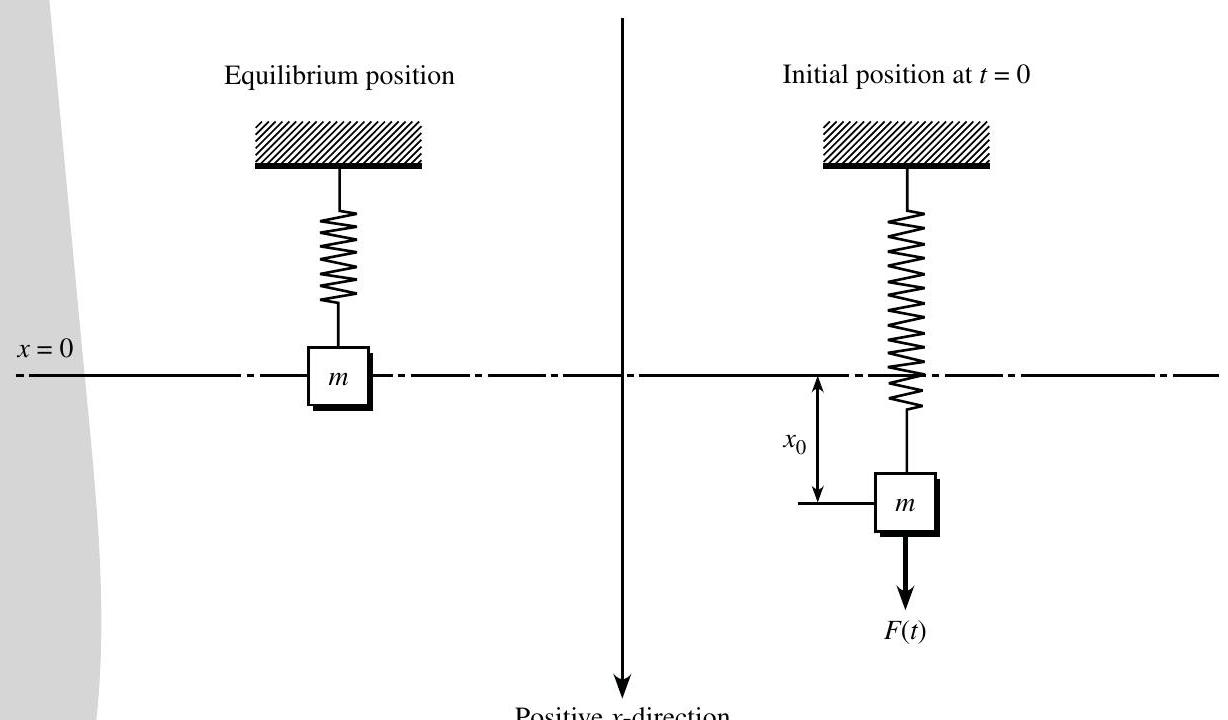
\includegraphics[max width=\textwidth]{2024_04_03_5bb5b4275a64cb9887d1g-132}
\end{center}

Positive $x$-direction

Fig. 14.1

Hooke's law: The restoring force $F$ of a spring is equal and opposite to the forces applied to the spring and is proportional to the extension (contraction) $l$ of the spring as a result of the applied force; that is, $F=-k l$, where $k$ denotes the constant of proportionality, generally called the spring constant.

Example 14.1. A steel ball weighing $128 \mathrm{lb}$ is suspended from a spring, whereupon the spring is stretched $2 \mathrm{ft}$ from its natural length. The applied force responsible for the 2-ft displacement is the weight of the ball, $128 \mathrm{lb}$. Thus, $F=-128 \mathrm{lb}$. Hooke's law then gives $-128=-k(2)$, or $k=64 \mathrm{lb} / \mathrm{ft}$.

For convenience, we choose the downward direction as the positive direction and take the origin to be the center of gravity of the mass in the equilibrium position. We assume that the mass of the spring is negligible and can be neglected and that air resistance, when present, is proportional to the velocity of the mass. Thus, at any time $t$, there are three forces acting on the system: (1) $F(t)$, measured in the positive direction; (2) a restoring force given by Hooke's law as $F_{s}=-k x, k>0$; and (3) a force due to air resistance given by $F_{a}=-a \dot{x}, a>0$, where $a$ is the constant of proportionality. Note that the restoring force $F_{s}$ always acts in a direction that will tend to return the system to the equilibrium position: if the mass is below the equilibrium position, then $x$ is positive and $-k x$ is negative; whereas if the mass is above the equilibrium position, then $x$ is negative and $-k x$ is positive. Also note that because $a>0$ the force $F_{a}$ due to air resistance acts in the opposite direction of the velocity and thus tends to retard, or damp, the motion of the mass.

It now follows from Newton's second law (see Chapter 7) that $m \ddot{x}=-k x-a \dot{x}+F(t)$, or


\begin{equation*}
\ddot{x}+\frac{a}{m} \dot{x}+\frac{k}{m} x=\frac{F(t)}{m} \tag{14.1}
\end{equation*}


If the system starts at $t=0$ with an initial velocity $v_{0}$ and from an initial position $x_{0}$, we also have the initial conditions


\begin{equation*}
x(0)=x_{0} \quad \dot{x}(0)=v_{0} \tag{14.2}
\end{equation*}


(See Problems 14.1-14.10.)

The force of gravity does not explicitly appear in (14.1), but it is present nonetheless. We automatically compensated for this force by measuring distance from the equilibrium position of the spring. If one wishes to exhibit gravity explicitly, then distance must be measured from the bottom end of the natural length of the spring. That is, the motion of a vibrating spring can be given by

$$
\ddot{x}+\frac{a}{m} \dot{x}+\frac{k}{m} x=g+\frac{F(t)}{m}
$$

if the origin, $x=0$, is the terminal point of the unstretched spring before the mass $m$ is attached.

\section*{ELECTRICAL CIRCUIT PROBLEMS}
The simple electrical circuit shown in Fig. 14-2 consists of a resistor $R$ in ohms; a capacitor $C$ in farads; an inductor $L$ in henries; and an electromotive force (emf) $E(t)$ in volts, usually a battery or a generator, all

\begin{center}
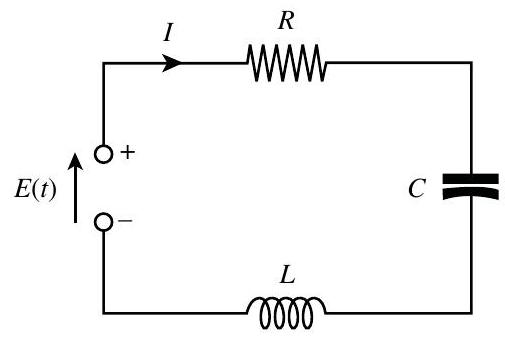
\includegraphics[max width=\textwidth]{2024_04_03_5bb5b4275a64cb9887d1g-133}
\end{center}

Fig. 14.2\\
connected in series. The current $I$ flowing through the circuit is measured in amperes and the charge $q$ on the capacitor is measured in coulombs.

Kirchhoff's loop law: The algebraic sum of the voltage drops in a simple closed electric circuit is zero.

It is known that the voltage drops across a resistor, a capacitor, and an inductor are respectively $R I,(1 / C) q$, and $L(d I / d t)$ where $q$ is the charge on the capacitor. The voltage drop across an emf is $-E(t)$. Thus, from Kirchhoff's loop law, we have


\begin{equation*}
R I+L \frac{d I}{d t}+\frac{1}{C} q-E(t)=0 \tag{14.3}
\end{equation*}


The relationship between $q$ and $I$ is


\begin{equation*}
I=\frac{d q}{d t} \quad \frac{d I}{d t}=\frac{d^{2} q}{d t^{2}} \tag{14.4}
\end{equation*}


Substituting these values into (14.3), we obtain


\begin{equation*}
\frac{d^{2} q}{d t^{2}}+\frac{R}{L} \frac{d q}{d t}+\frac{1}{L C} q=\frac{1}{L} E(t) \tag{14.5}
\end{equation*}


The initial conditions for $q$ are


\begin{equation*}
q(0)=\left.q_{0} \quad \frac{d q}{d t}\right|_{t=0}=I(0)=I_{0} \tag{14.6}
\end{equation*}


To obtain a differential equation for the current, we differentiate Eq. (14.3) with respect to $t$ and then substitute Eq. (14.4) directly into the resulting equation to obtain


\begin{equation*}
\frac{d^{2} I}{d t^{2}}+\frac{R}{L} \frac{d I}{d t}+\frac{1}{L C} I=\frac{1}{L} \frac{d E(t)}{d t} \tag{14.7}
\end{equation*}


The first initial condition is $I(0)=I_{0}$. The second initial condition is obtained from Eq. (14.3) by solving for $d I / d t$ and then setting $t=0$. Thus,


\begin{equation*}
\left.\frac{d I}{d t}\right|_{t=0}=\frac{1}{L} E(0)-\frac{R}{L} I_{0}-\frac{1}{L C} q_{0} \tag{14.8}
\end{equation*}


An expression for the current can be gotten either by solving Eq. (14.7) directly or by solving Eq. (14.5) for the charge and then differentiating that expression. (See Problems 14.12-14.16.)

\section*{BUOYANCY PROBLEMS}
Consider a body of mass $m$ submerged either partially or totally in a liquid of weight density $\rho$. Such a body experiences two forces, a downward force due to gravity and a counter force governed by:

Archimedes' principle: A body in liquid experiences a buoyant upward force equal to the weight of the liquid displaced by that body.

Equilibrium occurs when the buoyant force of the displaced liquid equals the force of gravity on the body. Figure 14-3 depicts the situation for a cylinder of radius $r$ and height $H$ where $h$ units of cylinder height are submerged at equilibrium. At equilibrium, the volume of water displaced by the cylinder is $\pi r^{2} h$, which provides a buoyant force of $\pi r^{2} h \rho$ that must equal the weight of the cylinder $m g$. Thus,


\begin{equation*}
\pi r^{2} h p=m g \tag{14.9}
\end{equation*}


\begin{center}
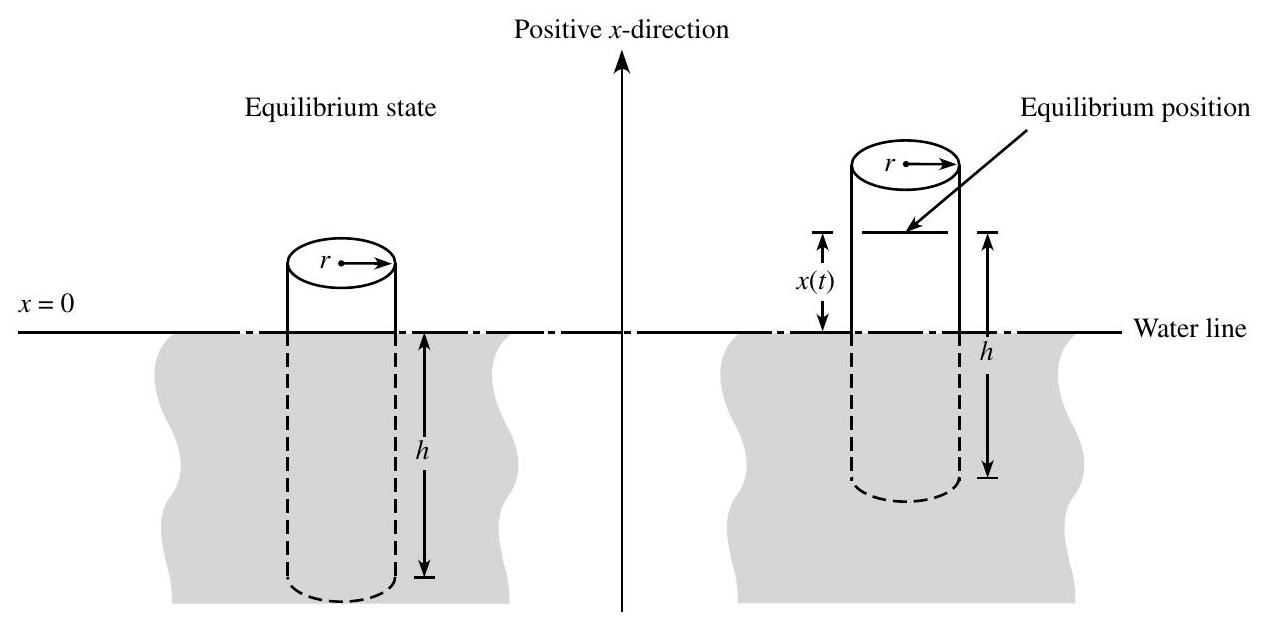
\includegraphics[max width=\textwidth]{2024_04_03_5bb5b4275a64cb9887d1g-135}
\end{center}

Fig. 14.3

Motion will occur when the cylinder is displaced from its equilibrium position. We arbitrarily take the upward direction to be the positive $x$-direction. If the cylinder is raised out of the water by $x(t)$ units, as shown in Fig. 14-3, then it is no longer in equilibrium. The downward or negative force on such a body remains $m g$ but the buoyant or positive force is reduced to $\pi r^{2}[h-x(t)] \rho$. It now follows from Newton's second law that

$$
m \ddot{x}=\pi r^{2}[h-x(t)] \rho-m g
$$

Substituting (14.9) into this last equation, we can simplify it to

or


\begin{gather*}
m \ddot{x}=-\pi r^{2} x(t) \rho \\
\ddot{x}+\frac{\pi r^{2} \rho}{m} x=0 \tag{14.10}
\end{gather*}


(See Problems 14.19-14.24.)

\section*{CLASSIFYING SOLUTIONS}
Vibrating springs, simple electrical circuits, and floating bodies are all governed by second-order linear differential equations with constant coefficients of the form


\begin{equation*}
\ddot{x}+a_{1} \dot{x}+a_{0} x=f(t) \tag{14.11}
\end{equation*}


For vibrating spring problems defined by Eq. (14.1), $a_{1}=a / m, a_{0}=k / m$, and $f(t)=F(t) / m$. For buoyancy problems defined by Eq. (14.10), $a_{1}=0, a_{0}=\pi r^{2} \rho / m$, and $f(t) \equiv 0$. For electrical circuit problems, the independent variable $x$ is replaced either by $q$ in Eq. (14.5) or $I$ in Eq. (14.7).

The motion or current in all of these systems is classified as free and undamped when $f(t) \equiv 0$ and $a_{1}=0$. It is classified as free and damped when $f(t)$ is identically zero but $a_{1}$ is not zero. For damped motion, there are three separate cases to consider, depending on whether the roots of the associated characteristic equation (see Chapter 9) are (1) real and distinct, (2) equal, or (3) complex conjugate. These cases are respectively classified as (1) overdamped, (2) critically damped, and (3) oscillatory damped (or, in electrical problems, underdamped). If $f(t)$ is not identically zero, the motion or current is classified as forced.

A motion or current is transient if it "dies out" (that is, goes to zero) as $t \rightarrow \infty$. A steady-state motion or current is one that is not transient and does not become unbounded. Free damped systems always yield transient\\
motions, while forced damped systems (assuming the external force to be sinusoidal) yield both transient and steady-state motions.

Free undamped motion defined by Eq. (14.11) with $a_{1}=0$ and $f(t) \equiv 0$ always has solutions of the form


\begin{equation*}
x(t)=c_{1} \cos \omega t+c_{2} \sin \omega t \tag{14.12}
\end{equation*}


which defines simple harmonic motion. Here $c_{1}, c_{2}$, and $\omega$ are constants with $\omega$ often referred to as circular frequency. The natural frequency $f$ is

$$
f=\frac{\omega}{2 \pi}
$$

and it represents the number of complete oscillations per time unit undertaken by the solution. The period of the system of the time required to complete one oscillation is

$$
T=\frac{1}{f}
$$

Equation (14.12) has the alternate form


\begin{equation*}
x(t)=(-1)^{k} A \cos (\omega t-\phi) \tag{14.13}
\end{equation*}


where the amplitude $A=\sqrt{c_{1}^{2}+c_{2}^{2}}$, the phase angle $\phi=\arctan \left(c_{2} / c_{1}\right)$, and $k$ is zero when $c_{1}$ is positive and unity when $c_{1}$ is negative.

\section*{Solved Problems}
14.1. A steel ball weighing $128 \mathrm{lb}$ is suspended from a spring, whereupon the spring is stretched $2 \mathrm{ft}$ from its natural length. The ball is started in motion with no initial velocity by displacing it 6 in above the equilibrium position. Assuming no air resistance, find (a) an expression for the position of the ball at any time $t$, and $(b)$ the position of the ball at $t=\pi / 12 \mathrm{sec}$.

(a) The equation of motion is governed by Eq. (14.1). There is no externally applied force, so $F(t)=0$, and no resistance from the surrounding medium, so $a=0$. The motion is free and undamped. Here $g=32 \mathrm{ft} / \mathrm{sec}^{2}$, $m=128 / 32=4$ slugs, and it follows from Example 14.1 that $k=64 \mathrm{lb} / \mathrm{ft}$. Equation (14.1) becomes $\ddot{x}+16 x=0$. The roots of its characteristic equation are $\lambda= \pm 4 i$, so its solution is


\begin{equation*}
x(t)=c_{1} \cos 4 t+c_{2} \sin 4 t \tag{1}
\end{equation*}


At $t=0$, the position of the ball is $x_{0}=-\frac{1}{2} \mathrm{ft}$ (the minus sign is required because the ball is initially displaced above the equilibrium position, which is in the negative direction). Applying this initial condition to (1), we find that

$$
-\frac{1}{2}=x(0)=c_{1} \cos 0+c_{2} \sin 0=c_{1}
$$

so (1) becomes


\begin{equation*}
x(t)=-\frac{1}{2} \cos 4 t+c_{2} \sin 4 t \tag{2}
\end{equation*}


The initial velocity is given as $v_{0}=0 \mathrm{ft} / \mathrm{sec}$. Differentiating (2), we obtain

$$
v(t)=\dot{x}(t)=2 \sin 4 t+4 c_{2} \cos 4 t
$$

whereupon

$$
0=v(0)=2 \sin 0+4 c_{2} \cos 0=4 c_{2}
$$

Thus, $c_{2}=0$, and (2) simplifies to


\begin{equation*}
x(t)=-\frac{1}{2} \cos 4 t \tag{3}
\end{equation*}


as the equation of motion of the steel ball at any time $t$.

(b) At $t=\pi / 12$,

$$
x\left(\frac{\pi}{12}\right)=-\frac{1}{2} \cos \frac{4 \pi}{12}=-\frac{1}{4} \mathrm{ft}
$$

14.2. A mass of $2 \mathrm{~kg}$ is suspended from a spring with a known spring constant of $10 \mathrm{~N} / \mathrm{m}$ and allowed to come to rest. It is then set in motion by giving it an initial velocity of $150 \mathrm{~cm} / \mathrm{sec}$. Find an expression for the motion of the mass, assuming no air resistance.

The equation of motion is governed by Eq. (14.1) and represents free undamped motion because there is no externally applied force on the mass, $F(t)=0$, and no resistance from the surrounding medium, $a=0$. The mass and the spring constant are given as $m=2 \mathrm{~kg}$ and $k=10 \mathrm{~N} / \mathrm{m}$, respectively, so Eq. (14.1) becomes $\ddot{x}+5 x=0$. The roots of its characteristic equation are purely imaginary, so its solution is


\begin{equation*}
x(t)=c_{1} \cos \sqrt{5} t+c_{2} \sin \sqrt{5} t \tag{1}
\end{equation*}


At $t=0$, the position of the ball is at the equilibrium position $x_{0}=0 \mathrm{~m}$. Applying this initial condition to (1), we find that

$$
0=x(0)=c_{1} \cos 0+c_{2} \sin 0=c_{1}
$$

whereupon (1) becomes


\begin{equation*}
x(t)=c_{2} \sin \sqrt{5} t \tag{2}
\end{equation*}


The initial velocity is given as $v_{0}=150 \mathrm{~cm} / \mathrm{sec}=1.5 \mathrm{~m} / \mathrm{sec}$. Differentiating (2), we obtain

$$
v(t)=\dot{x}(t)=\sqrt{5} c_{2} \cos \sqrt{5} t
$$

whereupon,

$$
1.5=v(0)=\sqrt{5} c_{2} \cos 0=\sqrt{5} c_{2} \quad c_{2}=\frac{1.5}{\sqrt{5}}=0.6708
$$

and (2) simplifies to


\begin{equation*}
x(t)=0.6708 \sin \sqrt{5} t \tag{3}
\end{equation*}


as the position of the mass at any time $t$.

14.3. Determine the circular frequency, natural frequency, and period for the simple harmonic motion described in Problem 14.2.

Circular frequency: $\quad \omega=\sqrt{5}=2.236 \mathrm{cycles} / \mathrm{sec}=2.236 \mathrm{~Hz}$

Natural frequency: $\quad f=\omega / 2 \pi=\frac{\sqrt{5}}{2 \pi}=0.3559 \mathrm{~Hz}$

Period:

$$
T=1 / f=\frac{2 \pi}{\sqrt{5}}=2.81 \mathrm{sec}
$$

14.4. Determine the circular frequency, natural frequency, and period for the simple harmonic motion described in Problem 14.1.

Circular frequency:

$$
\begin{gathered}
\omega=4 \text { cycles } / \mathrm{sec}=4 \mathrm{~Hz} \\
f=4 / 2 \pi=0.6366 \mathrm{~Hz} \\
T=1 / f=\pi / 2=1.57 \mathrm{sec}
\end{gathered}
$$

Natural frequency:

Period:

14.5. A $10-\mathrm{kg}$ mass is attached to a spring, stretching it $0.7 \mathrm{~m}$ from its natural length. The mass is started in motion from the equilibrium position with an initial velocity of $1 \mathrm{~m} / \mathrm{sec}$ in the upward direction. Find the subsequent motion, if the force due to air resistance is $-90 \dot{x} \mathrm{~N}$.

Taking $g=9.8 \mathrm{~m} / \mathrm{sec}^{2}$, we have $w=m g=98 \mathrm{~N}$ and $k=w / l=140 \mathrm{~N} / \mathrm{m}$. Furthermore, $a=90$ and $F(t) \equiv 0$ (there is no external force). Equation (14.1) becomes


\begin{equation*}
\ddot{x}+9 \dot{x}+14 x=0 \tag{1}
\end{equation*}


The roots of the associated characteristic equation are $\lambda_{1}=-2$ and $\lambda_{2}=-7$, which are real and distinct; hence this problem is an example of overdamped motion. The solution of (1) is

$$
x=c_{1} e^{-2 t}+c_{2} e^{-7 t}
$$

The initial conditions are $x(0)=0$ (the mass starts at the equilibrium position) and $\dot{x}(0)=-1$ (the initial velocity is in the negative direction). Applying these conditions, we find that $c_{1}=-c_{2}=-\frac{1}{5}$, so that $x=\frac{1}{5}\left(e^{-7 t}-e^{-2 t}\right)$. Note that $x \rightarrow 0$ as $t \rightarrow \infty$; thus, the motion is transient.

14.6. A mass of $1 / 4$ slug is attached to a spring, whereupon the spring is stretched $1.28 \mathrm{ft}$ from its natural length. The mass is started in motion from the equilibrium position with an initial velocity of $4 \mathrm{ft} / \mathrm{sec}$ in the downward direction. Find the subsequent motion of the mass if the force due to air resistance is $-2 \dot{x} \mathrm{lb}$.

Here $m=1 / 4, a=2, F(t) \equiv 0$ (there is no external force), and, from Hooke's law, $k=m g / l$ $=(1 / 4)(32) / 1.28=6.25$. Equation (14.1) becomes


\begin{equation*}
\ddot{x}+8 \dot{x}+25 x=0 \tag{1}
\end{equation*}


The roots of the associated characteristic equation are $\lambda_{1}=-4+i 3$ and $\lambda_{2}=-4-i 3$, which are complex conjugates; hence this problem is an example of oscillatory damped motion. The solution of $(1)$ is

$$
x=e^{-4 t}\left(c_{1} \cos 3 t+c_{2} \sin 3 t\right)
$$

The initial conditions are $x(0)=0$ and $\dot{x}(0)=4$. Applying these conditions, we find that $c_{1}=0$ and $c_{2}=\frac{4}{3}$; thus, $x=\frac{4}{3} e^{-4 t} \sin 3 t$. Since $x \rightarrow 0$ as $t \rightarrow \infty$, the motion is transient.

14.7. A mass of $1 / 4$ slug is attached to a spring having a spring constant of $1 \mathrm{lb} / \mathrm{ft}$. The mass is started in motion by initially displacing it $2 \mathrm{ft}$ in the downward direction and giving it an initial velocity of $2 \mathrm{ft} / \mathrm{sec}$ in the upward direction. Find the subsequent motion of the mass, if the force due to air resistance is $-1 \dot{x} \mathrm{lb}$.

Here $m=1 / 4, a=1, k=1$, and $F(t) \equiv 0$. Equation (14.1) becomes


\begin{equation*}
\ddot{x}+4 \dot{x}+4 x=0 \tag{1}
\end{equation*}


The roots of the associated characteristic equation are $\lambda_{1}=\lambda_{2}=-2$, which are equal; hence this problem is an example of critically damped motion. The solution of (I) is

$$
x=c_{1} e^{-2 t}+c_{2} t e^{-2 t}
$$

The initial conditions are $x(0)=2$ and $\dot{x}(0)=-2$ (the initial velocity is in the negative direction). Applying these conditions, we find that $c_{1}=c_{2}=2$. Thus,

$$
x=2 e^{-2 t}+2 t e^{-2 t}
$$

Since $x \rightarrow 0$ as $t \rightarrow \infty$, the motion is transient.

14.8. Show that the types of motions that result from free damped problems are completely determined by the quantity $a^{2}-4 \mathrm{~km}$.

For free damped motions $F(t) \equiv 0$ and Eq. (14.1) becomes

$$
\ddot{x}+\frac{a}{m} \dot{x}+\frac{k}{m} x=0
$$

The roots of the associated characteristic equation are

$$
\lambda_{1}=\frac{-a+\sqrt{a^{2}-4 k m}}{2 m} \quad \lambda_{2}=\frac{-a-\sqrt{a^{2}-4 k m}}{2 m}
$$

If $a^{2}-4 k m>0$, the roots are real and distinct; if $a^{2}-4 k m=0$, the roots are equal; if $a^{2}-4 k m<0$, the roots are complex conjugates. The corresponding motions are, respectively, overdamped, critically damped, and oscillatory damped. Since the real parts of both roots are always negative, the resulting motion in all three cases is transient. (For overdamped motion, we need only note that $\sqrt{a^{2}-4 k m}<a$, whereas for the other two cases the real parts are both $-a / 2 m$.)

14.9. A $10-\mathrm{kg}$ mass is attached to a spring having a spring constant of $140 \mathrm{~N} / \mathrm{m}$. The mass is started in motion from the equilibrium position with an initial velocity of $1 \mathrm{~m} / \mathrm{sec}$ in the upward direction and with an applied external force $F(t)=5 \sin t$. Find the subsequent motion of the mass if the force due to air resistance is $-90 \dot{x} \mathrm{~N}$.

Here $m=10, k=140, a=90$, and $F(t)=5 \sin t$. The equation of motion, (14.1), becomes


\begin{equation*}
\ddot{x}+9 \dot{x}+14 x=\frac{1}{2} \sin t \tag{1}
\end{equation*}


The general solution to the associated homogeneous equation $\ddot{x}+9 \dot{x}+14 x=0$ is (see Problem 14.5)

$$
x_{h}=c_{1} e^{-2 t}+c_{2} e^{-7 t}
$$

Using the method of undetermined coefficients (see Chapter 11), we find


\begin{equation*}
x_{p}=\frac{13}{500} \sin t-\frac{9}{500} \cos t \tag{2}
\end{equation*}


The general solution of ( 1 ) is therefore

$$
x=x_{h}+x_{p}=c_{1} e^{-2 t}+c_{2} e^{-7 t}+\frac{13}{500} \sin t-\frac{9}{500} \cos t
$$

Applying the initial conditions, $x(0)=0$ and $\dot{x}(0)=-1$, we obtain

$$
x=\frac{1}{500}\left(-90 e^{-2 t}+99 e^{-7 t}+13 \sin t-9 \cos t\right)
$$

Note that the exponential terms, which come from $x_{h}$ and hence represent an associated free overdamped motion, quickly die out. These terms are the transient part of the solution. The terms coming from $x_{p}$, however, do not die out as $t \rightarrow \infty$; they are the steady-state part of the solution.

14.10. A $128-\mathrm{lb}$ weight is attached to a spring having a spring constant of $64 \mathrm{lb} / \mathrm{ft}$. The weight is started in motion with no initial velocity by displacing it 6 in above the equilibrium position and by simultaneously applying to the weight an external force $F(t)=8 \sin 4 t$. Assuming no air resistance, find the subsequent motion of the weight.

Here $m=4, k=64, a=0$, and $F(t)=8 \sin 4 t$; hence, Eq. (14.1) becomes


\begin{equation*}
\ddot{x}+16 x=2 \sin 4 t \tag{1}
\end{equation*}


This problem is, therefore, an example of forced undamped motion. The solution to the associated homogeneous equation is

$$
x_{h}=c_{1} \cos 4 t+c_{2} \sin 4 t
$$

A particular solution is found by the method of undetermined coefficients (the modification described in Chapter 11 is necessary here): $x_{p}=-\frac{1}{4} \cos 4 t$. The solution to (1) is then

$$
x=c_{1} \cos 4 t+c_{2} \sin 4 t-\frac{1}{4} t \cos 4 t
$$

Applying the initial conditions, $x(0)=-\frac{1}{2}$ and $\dot{x}(0)=0$, we obtain

$$
x=-\frac{1}{2} \cos 4 t+\frac{1}{16} \sin 4 t-\frac{1}{4} t \cos 4 t
$$

Note that $|x| \rightarrow \infty$ as $t \rightarrow \infty$. This phenomenon is called pure resonance. It is due to the forcing function $F(t)$ having the same circular frequency as that of the associated free undamped system.

14.11. Write the steady-state motion found in Problem 14.9 in the form specified by Eq. (14.13).

The steady-state displacement is given by (2) of Problem 14.9 as

$$
x(t)=-\frac{9}{500} \cos t+\frac{13}{500} \sin t
$$

Its circular frequency is $\omega=1$. Here

$$
A=\sqrt{\left(\frac{13}{500}\right)^{2}+\left(-\frac{9}{500}\right)^{2}}=0.0316
$$

and

$$
\phi=\arctan \frac{13 / 500}{-9 / 500}=-0.965 \text { radians }
$$

The coefficient of the cosine term in the steady-state displacement is negative, so $k=1$, and Eq. (14.13) becomes

$$
x(t)=-0.0316 \cos (t+0.965)
$$

14.12. An RCL circuit connected in series has $R=180 \mathrm{ohms}, C=1 / 280$ farad, $L=20$ henries, and an applied voltage $E(t)=10 \sin t$. Assuming no initial charge on the capacitor, but an initial current of 1 ampere at $t=0$ when the voltage is first applied, find the subsequent charge on the capacitor.

Substituting the given quantities into Eq. (14.5), we obtain

$$
\ddot{q}+9 \dot{q}+14 q=\frac{1}{2} \sin t
$$

This equation is identical in form to (1) of Problem 14.9; hence, the solution must be identical in form to the solution of that equation. Thus,

$$
q=c_{1} e^{-2 t}+c_{2} e^{-7 t}+\frac{13}{500} \sin t-\frac{9}{500} \cos t
$$

Applying the initial conditions $q(0)=0$ and $\dot{q}(0)=1$, we obtain $c_{1}=110 / 500$ and $c_{2}=-101 / 500$. Hence,

$$
q=\frac{1}{500}\left(110 e^{-2 t}-101 e^{-7 t}+13 \sin t-9 \cos t\right)
$$

As in Problem 14.9, the solution is the sum of transient and steady-state terms.

14.13. An RCL circuit connected in series has $R=10 \mathrm{ohms}, C=10^{-2}$ farad, $L=\frac{1}{2}$ henry, and an applied voltage $E=12$ volts. Assuming no initial current and no initial charge at $t=0$ when the voltage is first applied, find the subsequent current in the system.

Substituting the given values into Eq. (14.7), we obtain the homogeneous equation [since $E(t)=12, d E / d t=0$ ]

$$
\frac{d^{2} I}{d t^{2}}+20 \frac{d I}{d t}+200 I=0
$$

The roots of the associated characteristic equation are $\lambda_{1}=-10+10 i$ and $\lambda_{2}=-10-10 i$; hence, this is an example of a free underdamped system for the current. The solution is


\begin{equation*}
I=e^{-10 t}\left(c_{1} \cos 10 t+c_{2} \sin 10 t\right) \tag{1}
\end{equation*}


The initial conditions are $I(0)=0$ and, from Eq. (14.8),

$$
\left.\frac{d I}{d t}\right|_{t=0}=\frac{12}{1 / 2}-\left(\frac{10}{1 / 2}\right)(0)-\frac{1}{(1 / 2)\left(10^{-2}\right)}(0)=24
$$

Applying these conditions to (1), we obtain $c_{1}=0$ and $c_{2}=\frac{12}{5}$; thus, $I=\frac{12}{5} e^{-10 t} \sin 10 t$, which is completely transient.

14.14. Solve Problem 14.13 by first finding the charge on the capacitor.

We first solve for the charge $q$ and then use $I=d q / d t$ to obtain the current. Substituting the values given in Problem 14.13 into Eq. (14.5), we have $\ddot{q}+20 \dot{q}+200 q=24$, which represents a forced system for the charge, in contrast to the free damped system obtained in Problem 14.3 for the current. Using the method of undetermined coefficients to find a particular solution, we obtain the general solution

$$
q=e^{-10 t}\left(c_{1} \cos 10 t+c_{2} \sin 10 t\right)+\frac{3}{25}
$$

Initial conditions for the charge are $q(0)=0$ and $\dot{q}(0)=0$; applying them, we obtain $c_{1}=c_{2}=-3 / 25$. Therefore,

$$
\begin{gathered}
q=-e^{-10 t}\left(\frac{3}{25} \cos 10 t+\frac{3}{25} \sin 10 t\right)+\frac{3}{25} \\
I=\frac{d q}{d t}=\frac{12}{5} e^{-10 t} \sin 10 t
\end{gathered}
$$

and

as before.

Note that although the current is completely transient, the charge on the capacitor is the sum of both transient and steady-state terms.

14.15. An RCL circuit connected in series has a resistance of $5 \mathrm{ohms}$, an inductance of 0.05 henry, a capacitor of $4 \times 10^{-4}$ farad, and an applied alternating emf of $200 \cos 100 t$ volts. Find an expression for the current flowing through this circuit if the initial current and the initial charge on the capacitor are both zero.

Here $R / L=5 / 0.05=100,1 /(L C)=1 /\left[0.05\left(4 \times 10^{-4}\right)\right]=50,000$, and

$$
\frac{1}{L} \frac{d E(t)}{d t}=\frac{1}{0.05} 200(-100 \sin 100 t)=-400,000 \sin 100 t
$$

so Eq. (14.7) becomes

$$
\frac{d^{2} I}{d t^{2}}+100 \frac{d I}{d t}+50,000 I=-400,000 \sin 100 t
$$

The roots of its characteristic equation are $-50 \pm 50 \sqrt{19} i$, hence the solution to the associated homogeneous problem is

$$
I_{h}=c_{1} e^{-50 t} \cos 50 \sqrt{19} t+c_{2} e^{-50 t} \sin 50 \sqrt{19} t
$$

Using the method of undetermined coefficients, we find a particular solution to be

$$
I_{p}=\frac{40}{17} \cos 100 t-\frac{160}{17} \sin 100 t
$$

so the general solution is


\begin{equation*}
I=I_{h}+I_{p}=c_{1} e^{-50 t} \cos 50 \sqrt{19} t+c_{2} e^{-50 t} \sin 50 \sqrt{19} t+\frac{40}{17} \cos 100 t-\frac{160}{17} \sin 100 t \tag{1}
\end{equation*}


The initial conditions are $I(0)=0$ and, from Eq. (14.8),

$$
\left.\frac{d I}{d t}\right|_{t=0}=\frac{200}{0.05}-\frac{5}{0.05}(0)-\frac{1}{0.05\left(4 \times 10^{-4}\right)}(0)=4000
$$

Applying the first of these conditions to (1) directly, we obtain

$$
0=I(0)=c_{1}(1)+c_{2}(0)+\frac{40}{17}
$$

or $c_{1}=-40 / 17=-2.35$. Substituting this value into (1) and then differentiating, we find that

$$
\begin{aligned}
& \frac{d I}{d t}=-2.35\left(-50 e^{-50 t} \cos 50 \sqrt{19} t-50 \sqrt{19} e^{-50 t} \sin 50 \sqrt{19} t\right) \\
& +c_{2}\left(-50 e^{-50 t} \sin 50 \sqrt{19} t+50 \sqrt{19} e^{-50 t} \cos 50 \sqrt{19} t\right)-\frac{4000}{17} \sin 100 t-\frac{16,000}{17} \cos 100 t \\
& \text { pon } 4000=\left.\frac{d I}{d t}\right|_{t=0}=-2.35(-50)+c_{2}(50 \sqrt{19})-\frac{16,000}{17}
\end{aligned}
$$

whereupon

and $c_{2}=22.13$. Equation (1) becomes

$$
I=-2.35 e^{-50 t} \cos 50 \sqrt{19} t+22.13 e^{-50 t} \sin 50 \sqrt{19} t+\frac{40}{17} \cos 100 t-\frac{160}{17} \sin 100 t
$$

14.16. Solve Problem 14.15 by first finding the charge on the capacitor.

Substituting the values given in Problem 14.15 into Eq. (14.5), we obtain

$$
\frac{d^{2} q}{d t^{2}}+100 \frac{d q}{d t}+50,000 q=4000 \cos 100 t
$$

The associated homogeneous equation is identical in form to the one in Problem 14.15, so it has the same solution (with $I_{h}$ replaced by $q_{h}$ ). Using the method of undetermined coefficients, we find a particular solution to be

$$
q_{p}=\frac{16}{170} \cos 100 t+\frac{4}{170} \sin 100 t
$$

so the general solution is


\begin{equation*}
q=q_{h}+q_{p}=c_{1} e^{-50 t} \cos 50 \sqrt{19} t+c_{2} e^{-50 t} \sin 50 \sqrt{19} t+\frac{16}{170} \cos 100 t+\frac{4}{170} \sin 100 t \tag{1}
\end{equation*}


The initial conditions on the charge are $q(0)=0$ and

$$
\left.\frac{d q}{d t}\right|_{t=0}=I(0)=0
$$

Applying the first of these conditions to (1) directly, we obtain

$$
0=q(0)=c_{1}(1)+c_{2}(0)+\frac{16}{170}
$$

or $c_{1}=-16 / 170=-0.0941$. Substituting this value into (1) and then differentiating, we find that


\begin{align*}
\frac{d q}{d t}= & -0.0941\left(-50 e^{-50 t} \cos 50 \sqrt{19} t-50 \sqrt{19} e^{-50 t} \sin 50 \sqrt{19} t\right) \\
& +c_{2}\left(-50 e^{-50 t} \sin 50 \sqrt{19} t+50 \sqrt{19} e^{-50 t} \cos 50 \sqrt{19} t\right)-\frac{160}{17} \sin 100 t+\frac{40}{17} \cos 100 t \tag{2}
\end{align*}


whereupon

$$
0=\left.\frac{d q}{d t}\right|_{t=0}=-0.0941(-50)+c_{2}(50 \sqrt{19})+\frac{40}{17}
$$

and $c_{2}=-0.0324$. Substituting this value into (2) and simplifying, we obtain as before


\begin{equation*}
I(t)=\frac{d q}{d t}=-2.35 e^{-50 t} \cos 50 \sqrt{19} t+22.13 e^{-50 t} \sin 50 \sqrt{19} t+\frac{40}{17} \cos 100 t-\frac{160}{17} \sin 100 t \tag{3}
\end{equation*}


14.17. Determine the circular frequency, the natural frequency, and the period of the steady-state current found in Problem 14.16.

The current is given by (3) of Problem 14.16. As $t \rightarrow \infty$, the exponential terms tend to zero, so the steady-state current is

$$
I(t)=\frac{40}{17} \cos 100 t-\frac{160}{17} \sin 100 t
$$

Circular frequency:

$$
\omega=100 \mathrm{~Hz}
$$

Natural frequency:

$$
f=\omega / 2 \pi=100 / 2 \pi=15.92 \mathrm{~Hz}
$$

Period:

$$
T=1 / f=2 \pi / 100=0.063 \mathrm{sec}
$$

14.18. Write the steady-state current found in Problem 14.17 in the form specified by Eq. (14.13).

The amplitude is

$$
A=\sqrt{\left(\frac{40}{17}\right)^{2}+\left(-\frac{160}{17}\right)^{2}}=9.701
$$

and the phase angle is

$$
\phi=\arctan \frac{-160 / 17}{40 / 17}=-1.326 \text { radians }
$$

The circular frequency is $\omega=100$. The coefficient of the cosine term is positive, so $k=0$ and Eq. (14.13) becomes

$$
I_{s}(t)=9.701 \cos (100 t+1.326)
$$

14.19. Determine whether a cylinder of radius $4 \mathrm{in}$, height $10 \mathrm{in}$, and weight $15 \mathrm{lb}$ can float in a deep pool of water of weight density $62.5 \mathrm{lb} / \mathrm{ft}^{3}$.

Let $h$ denote the length (in feet) of the submerged portion of the cylinder at equilibrium. With $r=\frac{1}{3} \mathrm{ft}$, it follows from Eq. (14.9) that

$$
h=\frac{m g}{\pi r^{2} \rho}=\frac{15}{\pi\left(\frac{1}{3}\right)^{2} 62.5}=0.688 \mathrm{ft}=8.25 \text { in }
$$

Thus, the cylinder will float with $10-8.25=1.75$ in of length above the water line at equilibrium.

14.20. Determine an expression for the motion of the cylinder described in Problem 14.19 if it is released with 20 percent of its length above the water line with a velocity of $5 \mathrm{ft} / \mathrm{sec}$ in the downward direction.

Here $r=\frac{1}{3} \mathrm{ft}, \rho=62.5 \mathrm{lb} / \mathrm{ft}^{3}, m=15 / 32$ slugs and Eq. (14.10) becomes

$$
\ddot{x}+46.5421 x=0
$$

The roots of the associated characteristic equation are $\pm \sqrt[i]{46.5421} i= \pm 6.82 i$; the general solution of the differential equation is


\begin{equation*}
x(t)=c_{1} \cos 6.82 t+c_{2} \sin 6.82 t \tag{1}
\end{equation*}


At $t=0,20$ percent of the 10-in length of the cylinder, or 2 in, is out of the water. Using the results of Problem 14.19, we know that the equilibrium position has 1.75 in above the water, so at $t=0$, the cylinder is raised $1 / 4$ in or $1 / 48 \mathrm{ft}$ above its equilibrium position. In the context of Fig. $14-3, x(0)=1 / 48 \mathrm{ft}$. The initial velocity is $5 \mathrm{ft} / \mathrm{sec}$ in the downward or negative direction in the coordinate system of Fig. 14-3, so $\dot{x}(0)=-5$. Applying these initial conditions to (1), we find that

$$
c_{1}=\frac{1}{48}=0.021 \text { and } c_{2}=\frac{-5}{6.82}=-0.73
$$

Equation (1) becomes

$$
x(t)=0.021 \cos 6.82 t-0.73 \sin 6.82 t
$$

14.21. Determine whether a cylinder of diameter $10 \mathrm{~cm}$, height $15 \mathrm{~cm}$, and weight $19.6 \mathrm{~N}$ can float in a deep pool of water of weight density 980 dynes $/ \mathrm{cm}^{3}$.

Let $h$ denote the length (in centimeters) of the submerged portion of the cylinder at equilibrium. With $r=5 \mathrm{~cm}$ and $m g=19.6 \mathrm{~N}=1.96 \times 10^{6}$ dynes, it follows from Eq. (14.9) that

$$
h=\frac{m g}{\pi r^{2} \rho}=\frac{1.96 \times 10^{6}}{\pi(5)^{2}(980)}=25.5 \mathrm{~cm}
$$

Since this is more height than the cylinder possesses, the cylinder cannot displace sufficient water to float and will sink to the bottom of the pool.

14.22. Determine whether a cylinder of diameter $10 \mathrm{~cm}$, height $15 \mathrm{~cm}$, and weight $19.6 \mathrm{~N}$ can float in a deep pool of liquid having weight density 2450 dynes $/ \mathrm{cm}^{3}$.

Let $h$ denote the length of the submerged portion of the cylinder at equilibrium. With $r=5 \mathrm{~cm}$ and $m g=19.6 \mathrm{~N}$ $=1.96 \times 10^{6}$ dynes, it follows from Eq. (14.9) that

$$
h=\frac{m g}{\pi r^{2} \rho}=\frac{1.96 \times 10^{6}}{\pi(5)^{2}(2450)}=10.2 \mathrm{~cm}
$$

Thus, the cylinder will float with $15-10.2=4.8 \mathrm{~cm}$ of length above the liquid at equilibrium.

14.23. Determine an expression for the motion of the cylinder described in Problem 14.22 if it is released at rest with $12 \mathrm{~cm}$ of its length fully submerged.

Here $r=5 \mathrm{~cm}, \rho=2450$ dynes $/ \mathrm{cm}^{3}, m=19.6 / 9.8=2 \mathrm{~kg}=2000 \mathrm{~g}$, and Eq. (14.10) becomes

$$
\ddot{x}+96.21 x=0
$$

The roots of the associated characteristic equation are $\pm \sqrt{96.21} i= \pm 9.8 i$; the general solution of the differential equation is


\begin{equation*}
x(t)=c_{1} \cos 9.81 t+c_{2} \sin 9.81 t \tag{1}
\end{equation*}


At $t=0,12 \mathrm{~cm}$ of the length of the cylinder is submerged. Using the results of Problem 14.22, we know that the equilibrium position has $10.2 \mathrm{~cm}$ submerged, so at $t=0$, the cylinder is submerged $12-10.2=1.8 \mathrm{~cm}$ below its equilibrium position. In the context of Fig. $14-3, x(0)=-1.8 \mathrm{~cm}$ with a negative sign indicating that the equilibrium line is submerged. The cylinder begins at rest, so its initial velocity is $\dot{x}(0)=0$. Applying these initial conditions to (1), we find that $c_{1}=-1.8$ and $c_{2}=0$. Equation (1) becomes

$$
x(t)=-1.8 \cos 9.81 t
$$

14.24. A solid cylinder partially submerged in water having weight density $62.5 \mathrm{lb} / \mathrm{ft}^{3}$, with its axis vertical, oscillates up and down within a period of $0.6 \mathrm{sec}$. Determine the diameter of the cylinder if it weighs $2 \mathrm{lb}$.

With $\rho=62.5 \mathrm{lb} / \mathrm{ft}^{3}$ and $m=2 / 32$ slugs, Eq. (14.10) becomes

$$
\ddot{x}+1000 \pi r^{2} x=0
$$

which has as its general solution


\begin{equation*}
x(t)=c_{1} \cos \sqrt{1000 \pi} r t+c_{2} \sin \sqrt{1000 \pi} r t \tag{1}
\end{equation*}


Its circular frequency is $\omega=r \sqrt{1000 \pi}$; its natural frequency is $f=\omega / 2 \pi=r \sqrt{250 / \pi}=8.92 r$; its period is $T=1 / f=1 / 8.92 r$. We are given $0.6=T=1 / 8.92 r$, thus $r=0.187 \mathrm{ft}=2.24$ in with a diameter of $4.48 \mathrm{in}$.

14.25. A prism whose cross section is an equilateral triangle with sides of length $l$ floats in a pool of liquid of weight density $\rho$ with its height parallel to the vertical axis. The prism is set in motion by displacing it from its equilibrium position (see Fig. 14-4) and giving it an initial velocity. Determine the differential equation governing the subsequent motion of this prism.

Equilibrium occurs when the buoyant force of the displaced liquid equals the force of gravity on the body. The area of an equilateral triangle with sides of length $l$ is $A=\sqrt{3} l^{2} / 4$. For the prism depicted in Fig. 14-4, with $h$ units of height submerged at equilibrium, the volume of water displaced at equilibrium is $\sqrt{3} l^{2} h / 4$, providing a buoyant force of $\sqrt{3} l^{2} h \rho / 4$. By Archimedes' principle, this buoyant force at equilibrium must equal the weight of the prism $m g$; hence,


\begin{equation*}
\sqrt{3} l^{2} h \rho / 4=m g \tag{1}
\end{equation*}


We arbitrarily take the upward direction to be the positive $x$-direction. If the prism is raised out of the water by $x(t)$ units, as shown in Fig. 14-4, then it is no longer in equilibrium. The downward or negative force on such a body remains $m g$ but the buoyant or positive force is reduced to $\sqrt{3} l^{2}[h-x(t)] \rho / 4$. It now follows from Newton's second law that

$$
m \ddot{x}=\frac{\sqrt{3} l^{2}[h-x(t)] \rho}{4}-m g
$$

Substituting (1) into this last equation, we simplify it to

$$
\ddot{x}+\frac{\sqrt{3} l^{2} \rho}{4 m} x=0
$$

\begin{center}
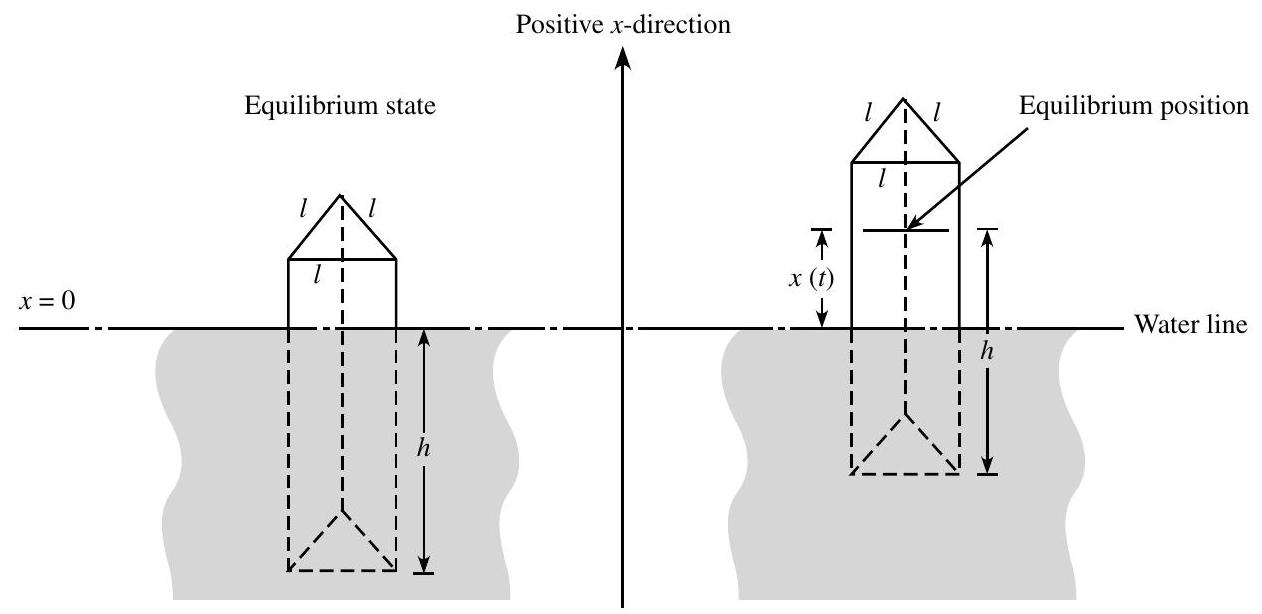
\includegraphics[max width=\textwidth]{2024_04_03_5bb5b4275a64cb9887d1g-145}
\end{center}

Fig. 14.4

\section*{Supplementary Problems}
14.26. A $10-\mathrm{lb}$ weight is suspended from a spring and stretches it 2 in from its natural length. Find the spring constant.

14.27. A mass of 0.4 slug is hung onto a spring and stretches it 9 in from its natural length. Find the spring constant.

14.28. A mass of $0.4 \mathrm{~g}$ is hung onto a spring and stretches it $3 \mathrm{~cm}$ from its natural length. Find the spring constant.

14.29. A mass of $0.3 \mathrm{~kg}$ is hung onto a spring and stretches it $15 \mathrm{~cm}$ from its natural length. Find the spring constant.

14.30. A 20 -lb weight is suspended from the end of a vertical spring having a spring constant of $40 \mathrm{lb} / \mathrm{ft}$ and is allowed to reach equilibrium. It is then set into motion by stretching the spring 2 in from its equilibrium position and releasing the mass from rest. Find the position of the weight at any time $t$ if there is no external force and no air resistance.

14.31. Solve Problem 14.30 if the weight is set in motion by compressing the spring by 2 in from its equilibrium position and giving it an initial velocity of $2 \mathrm{ft} / \mathrm{sec}$ in the downward direction.

14.32. A 20 -g mass is suspended from the end of a vertical spring having a spring constant of 2880 dynes $/ \mathrm{cm}$ and is allowed to reach equilibrium. It is then set into motion by stretching the spring $3 \mathrm{~cm}$ from its equilibrium position and releasing the mass with an initial velocity of $10 \mathrm{~cm} / \mathrm{sec}$ in the downward direction. Find the position of the mass at any time $t$ if there is no external force and no air resistance.

14.33. A $32-\mathrm{lb}$ weight is attached to a spring, stretching it $8 \mathrm{ft}$ from its natural length. The weight is started in motion by displacing it $1 \mathrm{ft}$ in the upward direction and by giving it an initial velocity of $2 \mathrm{ft} / \mathrm{sec}$ in the downward direction. Find the subsequent motion of the weight, if the medium offers negligible resistance.

14.34. Determine $(a)$ the circular frequency, $(b)$ the natural frequency, and $(c)$ the period for the vibrations described in Problem 14.31.

14.35. Determine $(a)$ the circular frequency, $(b)$ the natural frequency, and $(c)$ the period for the vibrations described in Problem 14.32.

14.36. Determine $(a)$ the circular frequency, $(b)$ the natural frequency, and $(c)$ the period for the vibrations described in Problem 14.33.

14.37. Find the solution to Eq. (14.1) with initial conditions given by Eq. (14.2) when the vibrations are free and undamped.

14.38. A $\frac{1}{4}$-slug mass is hung onto a spring, whereupon the spring is stretched 6 in from its natural length. The mass is then started in motion from the equilibrium position with an initial velocity of $4 \mathrm{ft} / \mathrm{sec}$ in the upward direction. Find the subsequent motion of the mass, if the force due to air resistance is $-2 \dot{x} \mathrm{lb}$.

14.39. A $\frac{1}{2}$-slug mass is attached to a spring so that the spring is stretched $2 \mathrm{ft}$ from its natural length. The mass is started in motion with no initial velocity by displacing it $\frac{1}{2} \mathrm{ft}$ in the upward direction. Find the subsequent motion of the mass, if the medium offers a resistance of $-4 \dot{x} \mathrm{lb}$.

14.40. A $\frac{1}{2}$-slug mass is attached to a spring having a spring constant of $6 \mathrm{lb} / \mathrm{ft}$. The mass is set into motion by displacing it 6 in below its equilibrium position with no initial velocity. Find the subsequent motion of the mass, if the force due to the medium is $-4 \dot{x} \mathrm{lb}$.

14.41. A $\frac{1}{2}-\mathrm{kg}$ mass is attached to a spring having a spring constant of $8 \mathrm{~N} / \mathrm{m}$. The mass is set into motion by displacing it $10 \mathrm{~cm}$ above its equilibrium position with an initial velocity of $2 \mathrm{~m} / \mathrm{sec}$ in the upward direction. Find the subsequent motion of the mass if the surrounding medium offers a resistance of $-4 \dot{x} \mathrm{~N}$.

14.42. Solve Problem 14.41 if instead the spring constant is $8.01 \mathrm{~N} / \mathrm{m}$.

14.43. Solve Problem 14.41 if instead the spring constant is $7.99 \mathrm{~N} / \mathrm{m}$.

14.44. A 1-slug mass is attached to a spring having a spring constant of $8 \mathrm{lb} / \mathrm{ft}$. The mass is initially set into motion from the equilibrium position with no initial velocity by applying an external force $F(t)=16 \cos 4 t$. Find the subsequent motion of the mass, if the force due to air resistance is $-4 \dot{x} \mathrm{lb}$.

14.45. A 64-lb weight is attached to a spring whereupon the spring is stretched $1.28 \mathrm{ft}$ and allowed to come to rest. The weight is set into motion by applying an external force $F(t)=4 \sin 2 t$. Find the subsequent motion of the weight if the surrounding medium offers a negligible resistance.

14.46. A $128-\mathrm{lb}$ weight is attached to a spring whereupon the spring is stretched $2 \mathrm{ft}$ and allowed to come to rest. The weight is set into motion from rest by displacing the spring 6 in above its equilibrium position and also by applying an external force $F(t)=8 \sin 4 t$. Find the subsequent motion of the weight if the surrounding medium offers a negligible resistance.

14.47. Solve Problem 14.38 if, in addition, the mass is subjected to an externally applied force $F(t)=16 \sin 8 t$.

14.48. A 16-lb weight is attached to a spring whereupon the spring is stretched $1.6 \mathrm{ft}$ and allowed to come to rest. The weight is set into motion from rest by displacing the spring 9 in above its equilibrium position and also by applying an external force $F(t)=5 \cos 2 t$. Find the subsequent motion of the weight if the surrounding medium offers a resistance of $-2 \dot{x} \mathrm{lb}$.

14.49. Write the steady-state portion of the motion found in Problem 14.48 in the form specified by Eq. (14.13).

14.50. A $\frac{1}{2}-\mathrm{kg}$ mass is attached to a spring having a spring constant of $6 \mathrm{~N} / \mathrm{m}$ and allowed to come to rest. The mass is set into motion by applying an external force $F(t)=24 \cos 3 t-33 \sin 3 t$. Find the subsequent motion of the mass if the surrounding medium offers a resistance of $-3 \dot{x} \mathrm{~N}$.

14.51. Write the steady-state portion of the motion found in Problem 14.50 in the form of Eq. (14.13).

14.52. An RCL circuit connected in series with $R=6 \mathrm{ohms}, C=0.02$ farad, and $L=0.1$ henry has an applied voltage $E(t)=6$ volts. Assuming no initial current and no initial charge at $t=0$ when the voltage is first applied, find the subsequent charge on the capacitor and the current in the circuit.

14.53. An RCL circuit connected in series with a resistance of $5 \mathrm{ohms}$, a condenser of capacitance $4 \times 10^{-4}$ farad, and an inductance of 0.05 henry has an applied emf $E(t)=110$ volts. Assuming no initial current and no initial charge on the capacitor, find expressions for the current flowing through the circuit and the charge on the capacitor at any time $t$.

14.54. An RCL circuit connected in series with $R=6 \mathrm{ohms}, C=0.02$ farad, and $L=0.1$ henry has no applied voltage. Find the subsequent current in the circuit if the initial charge on the capacitor is $\frac{1}{10}$ coulomb and the initial current is zero.

14.55. An RCL circuit connected in series with a resistance of $1000 \mathrm{ohm}$, a condenser of capacitance $4 \times 10^{-6} \mathrm{farad}$, and an inductance of 1 henry has an applied emf $E(t)=24$ volts. Assuming no initial current and no initial charge on the capacitor, find an expression for the current flowing through the circuit at any time $t$.

14.56. An RCL circuit connected in series with a resistance of 4 ohms, a capacitor of $1 / 26$ farad, and an inductance of $1 / 2$ henry has an applied voltage $E(t)=16 \cos 2 t$. Assuming no initial current and no initial charge on the capacitor, find an expression for the current flowing through the circuit at any time $t$.

14.57. Determine the steady-state current in the circuit described in Problem 14.56 and write it in the form of Eq. (14.13).

14.58. An RCL circuit connected in series with a resistance of $16 \mathrm{ohms}$, a capacitor of 0.02 farad, and an inductance of 2 henries has an applied voltage $E(t)=100 \sin 3 t$. Assuming no initial current and no initial charge on the capacitor, find an expression for the current flowing through the circuit at any time $t$.

14.59. Determine the steady-state current in the circuit described in Problem 14.56 and write it in the form of Eq. (14.13).

14.60. An RCL circuit connected in series with a resistance of $20 \mathrm{ohms}$, a capacitor of $10^{-4}$ farad, and an inductance of 0.05 henry has an applied voltage $E(t)=100 \cos 200 t$. Assuming no initial current and no initial charge on the capacitor, find an expression for the current flowing through the circuit at any time $t$.

14.61. Determine the steady-state current in the circuit described in Problem 14.60 and write it in the form of Eq. (14.13).

14.62. An RCL circuit connected in series with a resistance of 2 ohms, a capacitor of $1 / 260$ farad, and an inductance of 0.1 henry has an applied voltage $E(t)=100 \sin 60 t$. Assuming no initial current and no initial charge on the capacitor, find an expression for the charge on the capacitor at any time $t$.

14.63. Determine the steady-state charge on the capacitor in the circuit described in Problem 14.62 and write it in the form of Eq. (14.13).

14.64. An RCL circuit connected in series has $\mathrm{R}=5$ ohms, $C=10^{-2}$ farad, $L=\frac{1}{8}$ henry, and no applied voltage. Find the subsequent steady-state current in the circuit. Hint: Initial conditions are not needed.

14.65. An RCL circuit connected in series with $\mathrm{R}=5$ ohms, $C=10^{-2}$ farad, and $L=\frac{1}{8}$ henry has applied voltage $E(t)=\sin t$. Find the steady-state current in the circuit. Hint: Initial conditions are not needed.

14.66. Determine the equilibrium position of a cylinder of radius $3 \mathrm{in}$, height $20 \mathrm{in}$, and weight $5 \pi \mathrm{lb}$ that is floating with its axis vertical in a deep pool of water of weight density $62.5 \mathrm{lb} / \mathrm{ft}^{3}$.

14.67. Find an expression for the motion of the cylinder described in Problem 14.66 if it is disturbed from its equilibrium position by submerging an additional 2 in of height below the water line and with a velocity of $1 \mathrm{ft} / \mathrm{sec}$ in the downward direction.

14.68. Write the harmonic motion of the cylinder described in Problem 14.67 in the form of Eq. (14.13).

14.69. Determine the equilibrium position of a cylinder of radius $2 \mathrm{ft}$, height $4 \mathrm{ft}$, and weight $600 \mathrm{lb}$ that is floating with its axis vertical in a deep pool of water of weight density $62.5 \mathrm{lb} / \mathrm{ft}^{3}$.

14.70. Find an expression for the motion of the cylinder described in Problem 14.69 if it is released from rest with $1 \mathrm{ft}$ of its height submerged in water.

14.71. Determine (a) the circular frequency, (b) the natural frequency, and (c) the period for the vibrations described in Problem 14.70.

14.72. Determine (a) the circular frequency, (b) the natural frequency, and (c) the period for the vibrations described in Problem 14.67.

14.73. Determine the equilibrium position of a cylinder of radius $3 \mathrm{~cm}$, height $10 \mathrm{~cm}$, and mass $700 \mathrm{~g}$ that is floating with its axis vertical in a deep pool of water of mass density $1 \mathrm{~g} / \mathrm{cm}^{3}$.

14.74. Solve Problem 14.73 if the liquid is not water but another substance with mass density $2 \mathrm{~g} / \mathrm{cm}^{3}$.

14.75. Determine the equilibrium position of a cylinder of radius $30 \mathrm{~cm}$, height $500 \mathrm{~cm}$, and weight $2.5 \times 10^{7}$ dynes that is floating with its axis vertical in a deep pool of water of weight density 980 dynes $/ \mathrm{cm}^{3}$.

14.76. Find an expression for the motion of the cylinder described in Problem 14.75 if it is set in motion from its equilibrium position by striking it to produce an initial velocity of $50 \mathrm{~cm} / \mathrm{sec}$ in the downward direction.

14.77. Find the general solution to Eq. (14.10) and determine its period.

14.78. Determine the radius of a cylinder weighing $5 \mathrm{lb}$ with its axis vertical that oscillates in a pool of deep water $\left(\rho=62.5 \mathrm{lb} / \mathrm{ft}^{3}\right)$ with a period of $0.75 \mathrm{sec}$. Hint: Use the results of Problem 14.77.

14.79. Determine the weight of a cylinder having a diameter of $1 \mathrm{ft}$ with its axis vertical that oscillates in a pool of deep water $\left(\rho=62.5 \mathrm{lb} / \mathrm{ft}^{3}\right)$ with a period of $2 \mathrm{sec}$. Hint: Use the results of Problem 14.77.

14.80. A rectangular box of width $w$, length $l$, and height $h$ floats in a pool of liquid of weight density $\rho$ with its height parallel to the vertical axis. The box is set into motion by displacing it $x_{0}$ units from its equilibrium position and giving it an initial velocity of $v_{0}$. Determine the differential equation governing the subsequent motion of the box.

14.81. Determine (a) the period of oscillations for the motion described in Problem 14.80 and (b) the change in that period if the length of the box is doubled.

\section*{CHAPTER 15}
\section*{MATRICES AND VECTORS}
A matrix (designated by an uppercase boldface letter) is a rectangular array of elements arranged in horizontal rows and vertical columns. In this book, the elements of matrices will always be numbers or functions of the variable $t$. If all the elements are numbers, then the matrix is called a constant matrix.

Matrices will prove to be very helpful in several ways. For example, we can recast higher-order differential equations into a system of first-order differential equations using matrices (see Chapter 17). Matrix notation also provides a compact way of expressing solutions to differential equations (see Chapter 16).

\section*{Example 15.1.}
$$
\left[\begin{array}{ll}
1 & 2 \\
3 & 4
\end{array}\right],\left[\begin{array}{ccc}
1 & e^{t} & 2 \\
t & -1 & 1
\end{array}\right], \text { and }\left[\begin{array}{lll}
1 & t^{2} & \cos t
\end{array}\right]
$$

are all matrices. In particular, the first matrix is a constant matrix, whereas the last two are not.

A general matrix $\mathbf{A}$ having $p$ rows and $n$ columns is given by

$$
\mathbf{A}=\left[a_{i j}\right]=\left[\begin{array}{cccc}
a_{11} & a_{12} & \ldots & a_{1 n} \\
a_{21} & a_{22} & \ldots & a_{2 n} \\
\vdots & \vdots & & \vdots \\
a_{p 1} & a_{p 2} & \ldots & a_{p n}
\end{array}\right]
$$

where $a_{i j}$ represents that element appearing in the $i$ th row and $j$ th column. A matrix is square if it has the same number of rows and columns.

A vector (designated by a lowercase boldface letter) is a matrix having only one column or one row. (The third matrix given in Example 15.1 is a vector.)

\section*{MATRIX ADDITION}
The sum $\mathbf{A}+\mathbf{B}$ of two matrices $\mathbf{A}=\left[a_{i j}\right]$ and $\mathbf{B}=\left[b_{i j}\right]$ having the same number of rows and the same number of columns is the matrix obtained by adding the corresponding elements of $\mathbf{A}$ and $\mathbf{B}$. That is,

$$
\mathbf{A}+\mathbf{B}=\left[a_{i j}\right]+\left[b_{i j}\right]=\left[a_{i j}+b_{i j}\right]
$$

Matrix addition is both associative and commutative. Thus, $\mathbf{A}+(\mathbf{B}+\mathbf{C})=(\mathbf{A}+\mathbf{B})+\mathbf{C}$ and $\mathbf{A}+\mathbf{B}=\mathbf{B}+\mathbf{A}$.

\section*{SCALAR AND MATRIX MULTIPLICATION}
If $\lambda$ is either a number (also called a scalar) or a function of $t$, then $\lambda \mathbf{A}$ (or, equivalently, $\mathbf{A} \lambda$ ) is defined to be the matrix obtained by multiplying every element of $\mathbf{A}$ by $\lambda$. That is,

$$
\lambda \mathbf{A}=\lambda\left[a_{i j}\right]=\left[\lambda a_{i j}\right]
$$

Let $\mathbf{A}=\left[a_{i j}\right]$ and $\mathbf{B}=\left[b_{i j}\right]$ be two matrices such that $\mathbf{A}$ has $r$ rows and $n$ columns and $\mathbf{B}$ has $n$ rows and $p$ columns. Then the product $\mathbf{A B}$ is defined to be the matrix $\mathbf{C}=\left[c_{i j}\right]$ given by

$$
c_{i j}=\sum_{k=1}^{n} a_{i k} b_{k j} \quad(i=1,2, \ldots, r ; j=1,2, \ldots, p)
$$

The element $c_{i j}$ is obtained by multiplying the elements of the $i$ th row of $\mathbf{A}$ with the corresponding elements of the $j$ th column of $\mathbf{B}$ and summing the results.

Matrix multiplication is associative and distributes over addition; in general, however, it is not commutative. Thus,

$$
\mathbf{A}(\mathbf{B C})=(\mathbf{A B}) \mathbf{C}, \quad \mathbf{A}(\mathbf{B}+\mathbf{C})=\mathbf{A B}+\mathbf{A C}, \quad \text { and } \quad(\mathbf{B}+\mathbf{C}) \mathbf{A}=\mathbf{B A}+\mathbf{C A}
$$

but, in general, $\mathbf{A B} \neq \mathbf{B A}$.

\section*{POWERS OF A SQUARE MATRIX}
If $n$ is a positive integer and $\mathbf{A}$ is a square matrix, then

$$
\mathbf{A}^{n}=\underbrace{\mathbf{A} \mathbf{A} \cdots \mathbf{A}}_{n \text { times }}
$$

In particular, $\mathbf{A}^{2}=\mathbf{A A}$ and $\mathbf{A}^{3}=\mathbf{A A A}$. By definition, $\mathbf{A}^{0}=\mathbf{I}$, where

$$
\mathbf{I}=\left[\begin{array}{cccccc}
1 & 0 & 0 & \ldots & 0 & 0 \\
0 & 1 & 0 & \ldots & 0 & 0 \\
0 & 0 & 1 & \ldots & 0 & 0 \\
\vdots & & & \ddots & & \vdots \\
0 & 0 & 0 & \ldots & 1 & 0 \\
0 & 0 & 0 & \ldots & 0 & 1
\end{array}\right]
$$

is called an identity matrix. For any square matrix $\mathbf{A}$ and identity matrix $\mathbf{I}$ of the same size

$$
\mathbf{A I}=\mathbf{I A}=\mathbf{A}
$$

\section*{DIFFERENTIATION AND INTEGRATION OF MATRICES}
The derivative of $\mathbf{A}=\left[a_{i j}\right]$ is the matrix obtained by differentiating each element of $\mathbf{A}$; that is,

$$
\frac{d \mathbf{A}}{d t}=\left[\frac{d a_{i j}}{d t}\right]
$$

Similarly, the integral of $\mathbf{A}$, either definite or indefinite, is obtained by integrating each element of $\mathbf{A}$. Thus,

$$
\int_{a}^{b} \mathbf{A} d t=\left[\int_{a}^{b} a_{i j} d t\right] \text { and } \int \mathbf{A} d t=\left[\int a_{i j} d t\right]
$$

\section*{THE CHARACTERISTIC EQUATION}
The characteristic equation of a square matrix $\mathbf{A}$ is the polynomial equation in $\lambda$ given by


\begin{equation*}
\operatorname{det}(\mathbf{A}-\lambda \mathbf{I})=0 \tag{15.1}
\end{equation*}


where $\operatorname{det}(\quad)$ stands for "the determinant of." Those values of $\lambda$ which satisfy (15.1), that is, the roots of (15.1), are the eigenvalues of $\mathbf{A}$, a $k$-fold root being called an eigenvalue of multiplicity $k$.

Theorem 15.1. (Cayley-Hamilton theorem). Any square matrix satisfies its own characteristic equation. That is, if

then

$$
\begin{gathered}
\operatorname{det}(\mathbf{A}-\lambda \mathbf{I})=b_{n} \lambda^{n}+b_{n-1} \lambda^{n-1}+\cdots+b_{2} \lambda^{2}+b_{1} \lambda+b_{0} \\
b_{n} \mathbf{A}^{n}+b_{n-1} \mathbf{A}^{n-1}+\cdots+b_{2} \mathbf{A}^{2}+b_{1} \mathbf{A}+b_{0} \mathbf{I}=\mathbf{0}
\end{gathered}
$$

\section*{Solved Problems}
15.1. Show that $\mathbf{A}+\mathbf{B}=\mathbf{B}+\mathbf{A}$ for

$$
\begin{gathered}
\mathbf{A}=\left[\begin{array}{ll}
1 & 2 \\
3 & 4
\end{array}\right] \mathbf{B}=\left[\begin{array}{ll}
5 & 6 \\
7 & 8
\end{array}\right] \\
\mathbf{A}+\mathbf{B}=\left[\begin{array}{ll}
1 & 2 \\
3 & 4
\end{array}\right]+\left[\begin{array}{ll}
5 & 6 \\
7 & 8
\end{array}\right]=\left[\begin{array}{ll}
1+5 & 2+6 \\
3+7 & 4+8
\end{array}\right]=\left[\begin{array}{rr}
6 & 8 \\
10 & 12
\end{array}\right] \\
\mathbf{B}+\mathbf{A}=\left[\begin{array}{ll}
5 & 6 \\
7 & 8
\end{array}\right]+\left[\begin{array}{ll}
1 & 2 \\
3 & 4
\end{array}\right]=\left[\begin{array}{ll}
5+1 & 6+2 \\
7+3 & 8+4
\end{array}\right]=\left[\begin{array}{rr}
6 & 8 \\
10 & 12
\end{array}\right]
\end{gathered}
$$

Since the corresponding elements of the resulting matrices are equal, the desired equality follows.

15.2. Find $3 \mathbf{A}-\frac{1}{2} \mathbf{B}$ for the matrices given in Problem 15.1.

$$
\begin{aligned}
& 3 \mathbf{A}-\frac{1}{2} \mathbf{B}=3\left[\begin{array}{ll}
1 & 2 \\
3 & 4
\end{array}\right]+\left(-\frac{1}{2}\right)\left[\begin{array}{ll}
5 & 6 \\
7 & 8
\end{array}\right] \\
& =\left[\begin{array}{cc}
3 & 6 \\
9 & 12
\end{array}\right]+\left[\begin{array}{rr}
-\frac{5}{2} & -3 \\
-\frac{7}{2} & -4
\end{array}\right] \\
& =\left[\begin{array}{cc}
3+\left(-\frac{5}{2}\right) & 6+(-3) \\
9+\left(-\frac{7}{2}\right) & 12+(-4)
\end{array}\right]=\left[\begin{array}{cc}
\frac{1}{2} & 3 \\
\frac{11}{2} & 8
\end{array}\right]
\end{aligned}
$$

15.3. Find $\mathbf{A B}$ and $\mathbf{B A}$ for the matrices given in Problem 15.1.

$$
\begin{aligned}
& \mathbf{A B}=\left[\begin{array}{ll}
1 & 2 \\
3 & 4
\end{array}\right]+\left[\begin{array}{ll}
5 & 6 \\
7 & 8
\end{array}\right]=\left[\begin{array}{ll}
1(5)+2(7) & 1(6)+2(8) \\
3(5)+4(7) & 3(6)+4(8)
\end{array}\right]=\left[\begin{array}{ll}
19 & 22 \\
43 & 50
\end{array}\right] \\
& \mathbf{B A}=\left[\begin{array}{ll}
5 & 6 \\
7 & 8
\end{array}\right]+\left[\begin{array}{ll}
1 & 2 \\
3 & 4
\end{array}\right]=\left[\begin{array}{ll}
5(1)+6(3) & 5(2)+6(4) \\
7(1)+8(3) & 7(2)+8(4)
\end{array}\right]=\left[\begin{array}{ll}
23 & 34 \\
31 & 46
\end{array}\right]
\end{aligned}
$$

Note that for these matrices, $\mathbf{A B} \neq \mathbf{B A}$.

15.4. Find $(2 \mathbf{A}-\mathbf{B})^{2}$ for the matrices given in Problem 15.1.

$$
\begin{aligned}
& 2 \mathbf{A}-\mathbf{B}=2\left[\begin{array}{ll}
1 & 2 \\
3 & 4
\end{array}\right]+(-1)\left[\begin{array}{ll}
5 & 6 \\
7 & 8
\end{array}\right]=\left[\begin{array}{ll}
2 & 4 \\
6 & 8
\end{array}\right]+\left[\begin{array}{ll}
-5 & -6 \\
-7 & -8
\end{array}\right]=\left[\begin{array}{rr}
-3 & -2 \\
-1 & 0
\end{array}\right] \\
& \text { and } \quad \begin{aligned}
(2 \mathbf{A}-\mathbf{B})^{2} & =(2 \mathbf{A}-\mathbf{B})(2 \mathbf{A}-\mathbf{B})=\left[\begin{array}{ll}
-3 & -2 \\
-1 & 0
\end{array}\right]\left[\begin{array}{rr}
-3 & -2 \\
-1 & 0
\end{array}\right] \\
& =\left[\begin{array}{ll}
-3(-3)+(-2)(-1) & -3(-2)+(-2)(0) \\
-1(-3)+0(-1) & -1(-2)+0(0)
\end{array}\right]=\left[\begin{array}{rr}
11 & 6 \\
3 & 2
\end{array}\right]
\end{aligned}
\end{aligned}
$$

15.5. Find $\mathbf{A B}$ and $\mathbf{B A}$ for

$$
\mathbf{A}=\left[\begin{array}{lll}
1 & 2 & 3 \\
4 & 5 & 6
\end{array}\right], \quad \mathbf{B}=\left[\begin{array}{rr}
7 & 0 \\
8 & -1
\end{array}\right]
$$

Since $\mathbf{A}$ has three columns and $\mathbf{B}$ has two rows, the product $\mathbf{A B}$ is not defined. But

$$
\begin{aligned}
\mathbf{B A} & =\left[\begin{array}{rr}
7 & 0 \\
8 & -1
\end{array}\right]\left[\begin{array}{lll}
1 & 2 & 3 \\
4 & 5 & 6
\end{array}\right]=\left[\begin{array}{ccc}
7(1)+(0)(4) & 7(2)+(0)(5) & 7(3)+(0)(6) \\
8(1)+(-1)(4) & 8(2)+(-1)(5) & 8(3)+(-1)(6)
\end{array}\right] \\
& =\left[\begin{array}{lll}
7 & 14 & 21 \\
4 & 11 & 18
\end{array}\right]
\end{aligned}
$$

15.6. Find $\mathbf{A B}$ and $\mathbf{A C}$ if

$$
\begin{aligned}
\mathbf{A} & =\left[\begin{array}{rrr}
4 & 2 & 0 \\
2 & 1 & 0 \\
-2 & -1 & 1
\end{array}\right], \mathbf{B}=\left[\begin{array}{rrr}
2 & 3 & 1 \\
2 & -2 & -2 \\
-1 & 2 & 1
\end{array}\right], \quad \mathbf{C}=\left[\begin{array}{rrr}
3 & 1 & -3 \\
0 & 2 & 6 \\
-1 & 2 & 1
\end{array}\right] \\
\mathbf{A B} & =\left[\begin{array}{rrr}
4(2)+2(2)+(0)(-1) & 4(3)+2(-2)+(0)(2) & 4(1)+2(-2)+(0)(1) \\
2(2)+1(2)+(0)(-1) & 2(3)+1(-2)+(0)(2) & 2(1)+1(-2)+(0)(1) \\
-2(2)+(-1)(2)+1(-1) & -2(3)+(-1)(-2)+1(2) & -2(1)+(-1)(-2)+1(1)
\end{array}\right] \\
& =\left[\begin{array}{rrr}
12 & 8 & 0 \\
6 & 4 & 0 \\
-7 & -2 & 1
\end{array}\right] \\
\mathbf{A C} & =\left[\begin{array}{rrr}
4(3)+2(0)+(0)(-1) & 4(1)+2(2)+(0)(2) & 4(-3)+2(6)+(0)(1) \\
2(3)+1(0)+(0)(-1) & 2(1)+1(2)+(0)(2) & 2(-3)+1(6)+(0)(1) \\
-2(3)+(-1)(0)+1(-1) & -2(1)+(-1)(2)+1(2) & -2(-3)+(-1)(6)+1(1)
\end{array}\right] \\
& =\left[\begin{array}{ccc}
12 & 8 & 0 \\
6 & 4 & 0 \\
-7 & -2 & 1
\end{array}\right]
\end{aligned}
$$

Note that for these matrices $\mathbf{A B}=\mathbf{A C}$ and yet $\mathbf{B} \neq \mathbf{C}$. Therefore, the cancellation law is not valid for matrix multiplication.

\subsection*{15.7. Find $\mathbf{A x}$ if}
$$
\begin{gathered}
\mathbf{A}=\left[\begin{array}{llll}
1 & 2 & 3 & 4 \\
5 & 6 & 7 & 8
\end{array}\right] \quad \mathbf{x}=\left[\begin{array}{r}
9 \\
-1 \\
-2 \\
0
\end{array}\right] \\
\mathbf{A x}=\left[\begin{array}{c}
1(9)+2(-1)+3(-2)+4(0) \\
5(9)+6(-1)+7(-2)+8(0)
\end{array}\right]=\left[\begin{array}{c}
1 \\
25
\end{array}\right]
\end{gathered}
$$

15.8. Find $\frac{d \mathbf{A}}{d t}$ if $\mathbf{A}=\left[\begin{array}{cc}t^{2}+1 & e^{2 t} \\ \sin t & 45\end{array}\right]$.

$$
\frac{d \mathbf{A}}{d t}=\left[\begin{array}{ll}
\frac{d}{d t}\left(t^{2}+1\right) & \frac{d}{d t}\left(e^{2 t}\right) \\
\frac{d}{d t}(\sin t) & \frac{d}{d t}(45)
\end{array}\right]=\left[\begin{array}{cc}
2 t & 2 e^{2 t} \\
\cos t & 0
\end{array}\right]
$$

15.9. Find $\frac{d \mathbf{x}}{d t}$ if $\mathbf{x}=\left[\begin{array}{l}x_{1}(t) \\ x_{2}(t) \\ x_{3}(t)\end{array}\right]$.

$$
\frac{d \mathbf{x}}{d t}=\left[\begin{array}{c}
\frac{d x_{1}(t)}{d t} \\
\frac{d x_{2}(t)}{d t} \\
\frac{d x_{3}(t)}{d t}
\end{array}\right]=\left[\begin{array}{l}
\dot{x}_{1}(t) \\
\dot{x}_{2}(t) \\
\dot{x}_{3}(t)
\end{array}\right]
$$

15.10. Find $\int \mathbf{A} d t$ for $\mathbf{A}$ as given in Problem 15.8.

$$
\int \mathbf{A} d t=\left[\begin{array}{cc}
\int\left(t^{2}+1\right) d t & \int e^{2 t} d t \\
\int \sin t d t & \int 45 d t
\end{array}\right]=\left[\begin{array}{ll}
\frac{1}{3} t^{3}+t+c_{1} & \frac{1}{2} e^{2 t}+c_{2} \\
-\cos t+c_{3} & 45 t+c_{4}
\end{array}\right]
$$

15.11. Find $\int_{0}^{1} \mathbf{x} d t$ if $\mathbf{x}=\left[\begin{array}{c}1 \\ e^{t} \\ 0\end{array}\right]$.

$$
\int_{0}^{1} \mathbf{x} d t=\left[\begin{array}{c}
\int_{0}^{1} 1 d t \\
\int_{0}^{1} e^{t} d t \\
\int_{0}^{1} 0 d t
\end{array}\right]=\left[\begin{array}{c}
1 \\
e-1 \\
0
\end{array}\right]
$$

15.12. Find the eigenvalues of $\mathbf{A}=\left[\begin{array}{ll}1 & 3 \\ 4 & 2\end{array}\right]$.

We have

Hence,

$$
\begin{aligned}
\mathbf{A}-\lambda \mathbf{I} & =\left[\begin{array}{ll}
1 & 3 \\
4 & 2
\end{array}\right]+(-\lambda)\left[\begin{array}{ll}
1 & 0 \\
0 & 1
\end{array}\right] \\
= & {\left[\begin{array}{ll}
1 & 3 \\
4 & 2
\end{array}\right]+\left[\begin{array}{cc}
-\lambda & 0 \\
0 & -\lambda
\end{array}\right]=\left[\begin{array}{cc}
1-\lambda & 3 \\
4 & 2-\lambda
\end{array}\right] } \\
\operatorname{det}(\mathbf{A}-\lambda \mathbf{I}) & =\operatorname{det}\left[\begin{array}{cc}
1-\lambda & 3 \\
4 & 2-\lambda
\end{array}\right] \\
& =(1-\lambda)(2-\lambda)-(3)(4)=\lambda^{2}-3 \lambda-10
\end{aligned}
$$

The characteristic equation of $\mathbf{A}$ is $\lambda^{2}-3 \lambda-10=0$, which can be factored into $(\lambda-5)(\lambda+2)=0$. The roots of this equation are $\lambda_{1}=5$ and $\lambda_{2}=-2$, which are the eigenvalues of $\mathbf{A}$.

15.13. Find the eigenvalues of $\mathbf{A} t$ if $\mathbf{A}=\left[\begin{array}{rr}2 & 5 \\ -1 & -2\end{array}\right]$.

$$
\begin{aligned}
\mathbf{A} t-\lambda \mathbf{I} & =\left[\begin{array}{rr}
2 & 5 \\
-1 & -2
\end{array}\right] t+(-\lambda)\left[\begin{array}{ll}
1 & 0 \\
0 & 1
\end{array}\right] \\
& =\left[\begin{array}{rr}
2 t & 5 t \\
-t & -2 t
\end{array}\right]+\left[\begin{array}{rr}
-\lambda & 0 \\
0 & -\lambda
\end{array}\right]=\left[\begin{array}{cc}
2 t-\lambda & 5 t \\
-t & -2 t-\lambda
\end{array}\right] \\
\operatorname{det}(\mathbf{A}-\lambda \mathbf{I}) & =\operatorname{det}\left[\begin{array}{cc}
2 t-\lambda & 5 t \\
-t & -2 t-\lambda
\end{array}\right] \\
& =(2 t-\lambda)(-2 t-\lambda)-(5 t)(-t)=\lambda^{2}+t^{2}
\end{aligned}
$$

and the characteristic equation of $\mathbf{A} t$ is $\lambda^{2}+t^{2}=0$. The roots of this equation, which are the eigenvalues of $\mathbf{A} t$, are $\lambda_{1}=i t$ and $\lambda_{2}=-i t$, where $i=\sqrt{-1}$.

15.14. Find the eigenvalues of $\mathbf{A}=\left[\begin{array}{rrr}4 & 1 & 0 \\ -1 & 2 & 0 \\ 2 & 1 & -3\end{array}\right]$.

$$
\begin{aligned}
-\lambda \mathbf{I} & =\left[\begin{array}{rrr}
4 & 1 & 0 \\
-1 & 2 & 0 \\
2 & 1 & -3
\end{array}\right]-\lambda\left[\begin{array}{lll}
1 & 0 & 0 \\
0 & 1 & 0 \\
0 & 0 & 1
\end{array}\right] \\
& =\left[\begin{array}{ccc}
4-\lambda & 1 & 0 \\
-1 & 2-\lambda & 0 \\
2 & 1 & -3-\lambda
\end{array}\right]
\end{aligned}
$$

Thus,

$$
\begin{aligned}
\operatorname{det}(\mathbf{A}-\lambda \mathbf{I}) & =\operatorname{det}\left[\begin{array}{ccc}
4-\lambda & 1 & 0 \\
-1 & 2-\lambda & 0 \\
2 & 1 & -3-\lambda
\end{array}\right] \\
& =(-3-\lambda)[(4-\lambda)(2-\lambda)-(1)(-1)] \\
& =(-3-\lambda)(\lambda-3)(\lambda-3)
\end{aligned}
$$

The characteristic equation of $\mathbf{A}$ is

$$
(-3-\lambda)(\lambda-3)(\lambda-3)=0
$$

Hence, the eigenvalues of $\mathbf{A}$ are $\lambda_{1}=-3, \lambda_{2}=3$, and $\lambda_{3}=3$. Here $\lambda=3$ is an eigenvalue of multiplicity two, while $\lambda=-3$ is an eigenvalue of multiplicity one.

15.15. Find the eigenvalues of

$$
\begin{aligned}
& \mathbf{A}=\left[\begin{array}{rrrr}
5 & 7 & 0 & 0 \\
-3 & -5 & 0 & 0 \\
0 & 0 & -2 & 1 \\
0 & 0 & 0 & -2
\end{array}\right] \\
& \mathbf{A}-\lambda \mathbf{I}=\left[\begin{array}{cccc}
5-\lambda & 7 & 0 & 0 \\
-3 & -5-\lambda & 0 & 0 \\
0 & 0 & -2-\lambda & 1 \\
0 & 0 & 0 & -2-\lambda
\end{array}\right] \\
& \operatorname{det}(\mathbf{A}-\lambda \mathbf{I})=[(5-\lambda)(-5-\lambda)-(-3)(7)](-2-\lambda)(-2-\lambda) \\
& =\left(\lambda^{2}-4\right)(-2-\lambda)(-2-\lambda)
\end{aligned}
$$

and

The characteristic equation of $\mathbf{A}$ is

$$
\left(\lambda^{2}-4\right)(-2-\lambda)(-2-\lambda)=0
$$

which has roots $\lambda_{1}=2, \lambda_{2}=-2, \lambda_{3}=-2$, and $\lambda_{4}=-2$. Thus, $\lambda=-2$ is an eigenvalue of multiplicity three, whereas $\lambda=2$ is an eigenvalue of multiplicity one.

15.16. Verify the Cayley-Hamilton theorem for $\mathbf{A}=\left[\begin{array}{rr}2 & -7 \\ 3 & 6\end{array}\right]$.

For this matrix, we have $\operatorname{det}(\mathbf{A}-\lambda \mathbf{I})=\lambda^{2}-8 \lambda+33$; hence

$$
\begin{aligned}
\mathbf{A}^{2}-8 \mathbf{A}+33 \mathbf{I} & =\left[\begin{array}{rr}
2 & -7 \\
3 & 6
\end{array}\right]\left[\begin{array}{rr}
2 & -7 \\
3 & 6
\end{array}\right]-8\left[\begin{array}{rr}
2 & -7 \\
3 & 6
\end{array}\right]+33\left[\begin{array}{ll}
1 & 0 \\
0 & 1
\end{array}\right] \\
& =\left[\begin{array}{rr}
-17 & -56 \\
24 & 15
\end{array}\right]-\left[\begin{array}{rr}
16 & -56 \\
24 & 48
\end{array}\right]+\left[\begin{array}{rr}
33 & 0 \\
0 & 33
\end{array}\right] \\
& =\left[\begin{array}{ll}
0 & 0 \\
0 & 0
\end{array}\right]
\end{aligned}
$$

15.17. Verify the Cayley-Hamilton theorem for the matrix of Problem 15.14.

For this matrix, we found $\operatorname{det}(\mathbf{A}-\lambda \mathbf{I})=-(\lambda+3)(\lambda-3)^{2}$; hence

$$
\begin{aligned}
-(\mathbf{A}+3 \mathbf{I})(\mathbf{A}-3 \mathbf{I})^{2} & =-\left[\begin{array}{rrr}
7 & 1 & 0 \\
-1 & 5 & 0 \\
2 & 1 & 0
\end{array}\right]\left[\begin{array}{rrr}
1 & 1 & 0 \\
-1 & -1 & 0 \\
2 & 1 & -6
\end{array}\right]^{2} \\
& =-\left[\begin{array}{rrr}
7 & 1 & 0 \\
-1 & 5 & 0 \\
2 & 1 & 0
\end{array}\right]\left[\begin{array}{rrr}
0 & 0 & 0 \\
0 & 0 & 0 \\
-11 & -5 & 36
\end{array}\right]=\left[\begin{array}{lll}
0 & 0 & 0 \\
0 & 0 & 0 \\
0 & 0 & 0
\end{array}\right]
\end{aligned}
$$

\section*{Supplementary Problems}
In Problems 15.18 through 15.38, let

$$
\begin{gathered}
\mathbf{A}=\left[\begin{array}{rr}
2 & 3 \\
-1 & -2
\end{array}\right] \quad \mathbf{B}=\left[\begin{array}{rr}
1 & -4 \\
3 & 1
\end{array}\right] \quad \mathbf{C}=\left[\begin{array}{rrr}
3 & 5 & 0 \\
-2 & -3 & 0 \\
1 & 1 & 1
\end{array}\right] \\
\mathbf{D}=\left[\begin{array}{lll}
1 & 0 & 2 \\
1 & 0 & 1 \\
2 & 0 & 4
\end{array}\right] \quad \mathbf{x}=\left[\begin{array}{r}
1 \\
-2
\end{array}\right] \quad \mathbf{y}=\left[\begin{array}{l}
1 \\
1 \\
2
\end{array}\right]
\end{gathered}
$$

15.18. Find $\mathbf{A}+\mathbf{B}$.

15.19. Find $3 \mathbf{A}-2 \mathbf{B}$.

15.20. Find $\mathbf{C}-\mathbf{D}$.

15.21. Find $2 \mathrm{C}+5 \mathrm{D}$.

15.22. Find $\mathbf{A}+\mathbf{D}$.

15.23. Find $\mathbf{x}-3 \mathbf{y}$.

15.24. Find (a) $\mathbf{A B}$ and (b) BA.

15.25. Find $\mathbf{A}^{2}$.

15.26. Find $\mathbf{A}^{7}$.

15.27. Find $\mathbf{B}^{2}$.

15.28. Find (a) CD and (b) DC.

15.29. Find (a) Ax and (b) $\mathbf{x A}$.

15.30. Find $\mathbf{A C}$.

15.31. Find $(\mathbf{C}+\mathbf{D}) \mathbf{y}$.

15.32. Find the characteristic equation and eigenvalues of $\mathbf{A}$.

15.33. Find the characteristic equation and eigenvalues of $\mathbf{B}$.

15.34. Find the characteristic equation and eigenvalues of $\mathbf{A}+\mathbf{B}$.

15.35. Find the characteristic equation and eigenvalues of $3 \mathbf{A}$.

15.36. Find the characteristic equation and eigenvalues of $\mathbf{A}+5 \mathbf{I}$.

15.37. Find the characteristic equation and the eigenvalues of $\mathbf{C}$. Determine the multiplicity of each eigenvalue.

15.38. Find the characteristic equation and the eigenvalues of $\mathbf{D}$. Determine the multiplicity of each eigenvalue.

15.39. Find the characteristic equation and the eigenvalues of $\mathbf{A}=\left[\begin{array}{ll}t & t^{2} \\ 1 & 2 t\end{array}\right]$.

15.40. Find the characteristic equation and the eigenvalues of $\mathbf{A}=\left[\begin{array}{ccc}t & 6 t & 0 \\ 4 t & -t & 0 \\ 0 & 1 & 5 t\end{array}\right]$.

15.41. Find $\frac{d \mathbf{A}}{d t}$ for $\mathbf{A}$ as given in Problem 15.39 .

15.42. Find $\frac{d \mathbf{A}}{d t}$ for $\mathbf{A}=\left[\begin{array}{c}\cos 2 t \\ t e^{3 t^{2}}\end{array}\right]$.

15.43. Find $\int_{0}^{1} \mathbf{A} d t$ for $\mathbf{A}$ as given in Problem 15.42 .

\section*{CHAPTER 16}
\section*{DEFINITION}
For a square matrix $\mathbf{A}$,


\begin{equation*}
e^{\mathbf{A} t} \equiv \mathbf{I}+\frac{1}{1 !} \mathbf{A} t+\frac{1}{2 !} \mathbf{A}^{2} t^{2}+\cdots=\sum_{n=0}^{\infty} \frac{1}{n !} \mathbf{A}^{n} t^{n} \tag{16.1}
\end{equation*}


The infinite series (16.1) converges for every $\mathbf{A}$ and $t$, so that $e^{\mathbf{A} t}$ is defined for all square matrices.

\section*{COMPUTATION OF $e^{\text {At }}$}
For actually computing the elements of $e^{\mathbf{A} t},(16.1)$ is not generally useful. However, it follows (with some effort) from Theorem 15.1, applied to the matrix $\mathbf{A} t$, that the infinite series can be reduced to a polynomial in $t$. Thus:

Theorem 16.1. If $\mathbf{A}$ is a matrix having $n$ rows and $n$ columns, then


\begin{equation*}
e^{\mathbf{A} t}=\alpha_{n-1} \mathbf{A}^{n-1} t^{n-1}+\alpha_{n-2} \mathbf{A}^{n-2} t^{n-2}+\cdots+\alpha_{2} \mathbf{A}^{2} t^{2}+\alpha_{1} \mathbf{A} t+\alpha_{0} \mathbf{I} \tag{16.2}
\end{equation*}


where $\alpha_{0}, \alpha_{1}, \ldots, \alpha_{n-1}$ are functions of $t$ which must be determined for each $\mathbf{A}$.

Example 16.1. When $\mathbf{A}$ has two rows and two columns, then $n=2$ and


\begin{equation*}
e^{\mathbf{A} t}=\alpha_{1} \mathbf{A} t+\alpha_{0} \mathbf{I} \tag{16.3}
\end{equation*}


When $\mathbf{A}$ has three rows and three columns, then $n=3$ and


\begin{equation*}
e^{\mathbf{A} t}=\alpha_{2} \mathbf{A}^{2} t^{2}+\alpha_{1} \mathbf{A} t+\alpha_{0} \mathbf{I} \tag{16.4}
\end{equation*}


Theorem 16.2. Let $\mathbf{A}$ be as in Theorem 16.1, and define


\begin{equation*}
r(\lambda) \equiv \alpha_{n-1} \lambda^{n-1}+\alpha_{n-2} \lambda^{n-2}+\cdots+\alpha_{2} \lambda^{2}+\alpha_{1} \lambda+\alpha_{0} \tag{16.5}
\end{equation*}


Then if $\lambda_{i}$ is an eigenvalue of $\mathbf{A} t$,


\begin{equation*}
e^{\lambda i}=r\left(\lambda_{i}\right) \tag{16.6}
\end{equation*}


Furthermore, if $\lambda_{i}$ is an eigenvalue of multiplicity $k, k>1$, then the following equations are also valid:


\begin{align*}
e^{\lambda_{i}} & =\left.\frac{d}{d \lambda} r(\lambda)\right|_{\lambda=\lambda_{i}} \\
e^{\lambda_{i}} & =\left.\frac{d^{2}}{d \lambda^{2}} r(\lambda)\right|_{\lambda=\lambda_{i}} \tag{16.7}
\end{align*}


$$
e^{\lambda_{i}}=\left.\frac{d^{k-1}}{d \lambda^{k-1}} r(\lambda)\right|_{\lambda=\lambda_{i}}
$$

Note that Theorem 16.2 involves the eigenvalues of $\mathbf{A} t$; these are $t$ times the eigenvalues of $\mathbf{A}$. When computing the various derivatives in (16.7), one first calculates the appropriate derivatives of the expression (16.5) with respect to $\lambda$, and then substitutes $\lambda=\lambda_{i}$. The reverse procedure of first substituting $\lambda=\lambda_{i}$ (a function of $t$ ) into (16.5), and then calculating the derivatives with respect to $t$, can give erroneous results.

Example 16.2. Let $\mathbf{A}$ have four rows and four columns and let $\lambda=5 t$ and $\lambda=2 t$ be eigenvalues of $\mathbf{A} t$ of multiplicities three and one, respectively. Then $n=4$ and

$$
\begin{aligned}
r(\lambda) & =\alpha_{3} \lambda^{3}+\alpha_{2} \lambda^{2}+\alpha_{1} \lambda+\alpha_{0} \\
r^{\prime}(\lambda) & =3 \alpha_{3} \lambda^{2}+2 \alpha_{2} \lambda+\alpha_{1} \\
r^{\prime \prime}(\lambda) & =6 \alpha_{3} \lambda+2 \alpha_{2}
\end{aligned}
$$

Since $\lambda=5 t$ is an eigenvalue of multiplicity three, it follows that $e^{5 t}=r(5 t), e^{5 t}=r^{\prime}(5 t)$, and $e^{5 t}=r^{\prime \prime}(5 t)$. Thus,

$$
\begin{aligned}
e^{5 t} & =\alpha_{3}(5 t)^{3}+\alpha_{2}(5 t)^{2}+\alpha_{1}(5 t)+\alpha_{0} \\
e^{5 t} & =3 \alpha_{3}(5 t)^{2}+2 \alpha_{2}(5 t)^{2}+\alpha_{1} \\
e^{5 t} & =6 \alpha_{3}(5 t)+2 \alpha_{2}
\end{aligned}
$$

Also, since $\lambda=2 t$ is an eigenvalue of multiplicity one, it follows that $e^{2 t}=r(2 t)$, or

$$
e^{2 t}=\alpha_{3}(2 t)^{3}+\alpha_{2}(2 t)^{2}+\alpha_{1}(2 t)+\alpha_{0}
$$

Notice that we now have four equations in the four unknown $\alpha$ 's.

Method of computation: For each eigenvalue $\lambda_{t}$, of $\mathbf{A} t$, apply Theorem 16.2 to obtain a set of linear equations. When this is done for each eigenvalue, the set of all equations so obtained can be solved for $\alpha_{0}$, $\alpha_{1}, \ldots, \alpha_{n-1}$. These values are then substituted into Eq. (16.2), which, in turn, is used to compute $e^{\mathbf{A} t}$.

\section*{Solved Problems}
16.1. Find $e^{\mathbf{A} t}$ for $\mathbf{A}=\left[\begin{array}{ll}1 & 1 \\ 9 & 1\end{array}\right]$.

Here $n=2$. From Eq. (16.3),

\[
e^{\mathbf{A} t}=\alpha_{1} \mathbf{A} t+\alpha_{0} \mathbf{I}=\left[\begin{array}{cc}
\alpha_{1} t+\alpha_{0} & \alpha_{1} t  \tag{1}\\
9 \alpha_{1} t & \alpha_{1} t+\alpha_{0}
\end{array}\right]
\]

and from Eq. (16.5), $r(\lambda)=\alpha_{1} \lambda+\alpha_{0}$. The eigenvalues of $\mathbf{A} t$ are $\lambda_{1}=4 t$ and $\lambda_{2}=-2 t$, which are both of multiplicity one. Substituting these values successively into Eq. (16.6), we obtain the two equations

$$
\begin{gathered}
e^{4 t}=4 t \alpha_{1}+\alpha_{0} \\
e^{-2 t}=-2 t \alpha_{1}+\alpha_{0}
\end{gathered}
$$

Solving these equations for $\alpha_{1}$ and $\alpha_{0}$, we find that

$$
\alpha_{1}=\frac{1}{6 t}\left(e^{4 t}-e^{-2 t}\right) \quad \text { and } \quad \alpha_{0}=\frac{1}{3}\left(e^{4 t}+2 e^{-2 t}\right)
$$

Substituting these values into (1) and simplifying, we have

$$
e^{\mathbf{A} t}=\frac{1}{6}\left[\begin{array}{cc}
3 e^{4 t}+3 e^{-2 t} & e^{4 t}-e^{-2 t} \\
9 e^{4 t}-9 e^{-2 t} & 3 e^{4 t}+3 e^{-2 t}
\end{array}\right]
$$

16.2. Find $e^{\mathbf{A} t}$ for $\mathbf{A}=\left[\begin{array}{rr}0 & 1 \\ 8 & -2\end{array}\right]$.

Since $n=2$, it follows from Eqs. (16.3) and (16.5) that

\[
e^{\mathbf{A} t}=\alpha_{1} \mathbf{A} t+\alpha_{0} \mathbf{I}=\left[\begin{array}{cc}
\alpha_{0} & \alpha_{1} t  \tag{1}\\
8 \alpha_{1} t & -2 \alpha_{1} t+\alpha_{0}
\end{array}\right]
\]

and $r(\lambda)=\alpha_{1} \lambda+\alpha_{0}$. The eigenvalues of $\mathbf{A} t$ are $\lambda_{1}=2 t$ and $\lambda_{2}=-4 t$, which are both of multiplicity one. Substituting these values successively into (16.6), we obtain

$$
e^{2 t}=\alpha_{1}(2 t)+\alpha_{0} \quad e^{-4 t}=\alpha_{1}(-4 t)+\alpha_{0}
$$

Solving these equations for $\alpha_{1}$ and $\alpha_{0}$, we find that

$$
\alpha_{1}=\frac{1}{6 t}\left(e^{2 t}-e^{-4 t}\right) \quad \alpha_{0}=\frac{1}{3}\left(2 e^{2 t}+e^{-4 t}\right)
$$

Substituting these values into (1) and simplifying, we have

$$
e^{\mathbf{A} t}=\frac{1}{6}\left[\begin{array}{cc}
4 e^{2 t}+2 e^{-4 t} & e^{2 t}-e^{-4 t} \\
8 e^{2 t}-8 e^{-4 t} & 2 e^{2 t}+4 e^{-4 t}
\end{array}\right]
$$

16.3. Find $e^{\mathbf{A} t}$ for $\mathbf{A}=\left[\begin{array}{rr}0 & 1 \\ -1 & 0\end{array}\right]$.

Here $n=2$; hence,

\[
e^{\mathbf{A} t}=\alpha_{1} \mathbf{A} t+\alpha_{0} \mathbf{I}=\left[\begin{array}{cc}
\alpha_{0} & \alpha_{1} t  \tag{1}\\
-\alpha_{1} t & \alpha_{0}
\end{array}\right]
\]

and $r(\lambda)=\alpha_{1} \lambda+\alpha_{0}$. The eigenvalues of $\mathbf{A} t$ are $\lambda_{1}=i t$ and $\lambda_{2}=-i t$, which are both of multiplicity one. Substituting these values successively into Eq. (16.6), we obtain

$$
e^{i t}=\alpha_{1}(i t)+\alpha_{0} \quad e^{-i t}=\alpha_{1}(-i t)+\alpha_{0}
$$

Solving these equations for $\alpha_{1}$ and $\alpha_{0}$ and using Euler's relations, we find that

$$
\begin{aligned}
& \alpha_{1}=\frac{1}{2 i t}\left(e^{i t}-e^{-i t}\right)=\frac{\sin t}{t} \\
& \alpha_{0}=\frac{1}{2}\left(e^{i t}+e^{-i t}\right)=\cos t
\end{aligned}
$$

Substituting these values into (1), we obtain

$$
e^{\mathbf{A} t}=\left[\begin{array}{cc}
\cos t & \sin t \\
-\sin t & \cos t
\end{array}\right]
$$

16.4. Find $e^{\mathbf{A} t}$ for $\mathbf{A}=\left[\begin{array}{rr}0 & 1 \\ -9 & 6\end{array}\right]$.

Here $n=2$. From Eq. (16.3),

\[
e^{\mathbf{A} t}=\alpha_{1} \mathbf{A} t+\alpha_{0} \mathbf{I}=\left[\begin{array}{cc}
\alpha_{0} & \alpha_{1} t  \tag{1}\\
-9 \alpha_{1} t & 6 \alpha_{1} t+\alpha_{0}
\end{array}\right]
\]

and from Eq. (16.5), $r(\lambda)=\alpha_{1} \lambda+\alpha_{0}$. Thus, $d r(\lambda) / d \lambda=\alpha_{1}$. The eigenvalues of $\mathbf{A} t$ are $\lambda_{1}=\lambda_{2}=3 t$, which is a single eigenvalue of multiplicity two. It follows from Theorem 16.2 that

$$
\begin{aligned}
& e^{3 t}=3 t \alpha_{1}+\alpha_{0} \\
& e^{3 t}=\alpha_{1}
\end{aligned}
$$

Solving these equations for $\alpha_{1}$ and $\alpha_{0}$, we find that

$$
\alpha_{1}=e^{3 t} \quad \text { and } \quad \alpha_{0}=e^{3 t}(1-3 t)
$$

Substituting these values into (1) and simplifying, we have

$$
e^{\mathbf{A} t}=e^{3 t}\left[\begin{array}{cc}
1-3 t & t \\
-9 t & 1+3 t
\end{array}\right]
$$

16.5. Find $e^{\mathbf{A} t}$ for $\mathbf{A}=\left[\begin{array}{lll}3 & 1 & 0 \\ 0 & 3 & 1 \\ 0 & 0 & 3\end{array}\right]$.

Here $n=3$. From Eqs. (16.4) and (16.5) we have


\begin{align*}
e^{\mathbf{A} t} & =\alpha_{2} \mathbf{A}^{2} t^{2}+\alpha_{1} \mathbf{A} t+\alpha_{0} \mathbf{I} \\
& =\alpha_{2}\left[\begin{array}{lll}
9 & 6 & 1 \\
0 & 9 & 6 \\
0 & 0 & 9
\end{array}\right] t^{2}+\alpha_{1}\left[\begin{array}{lll}
3 & 1 & 0 \\
0 & 3 & 1 \\
0 & 0 & 3
\end{array}\right] t+\alpha_{0}\left[\begin{array}{ccc}
1 & 0 & 0 \\
0 & 1 & 0 \\
0 & 0 & 1
\end{array}\right] \\
& =\left[\begin{array}{ccc}
9 \alpha_{2} t^{2}+3 \alpha_{1} t+\alpha_{0} & 6 \alpha_{2} t^{2}+\alpha_{1} t & \alpha_{2} t^{2} \\
0 & 9 \alpha_{2} t^{2}+3 \alpha_{1} t+\alpha_{0} & 6 \alpha_{2} t^{2}+\alpha_{1} t \\
0 & 0 & 9 \alpha_{2} t^{2}+3 \alpha_{1} t+\alpha_{0}
\end{array}\right] \tag{1}
\end{align*}


and $r(\lambda)=\alpha_{2} \lambda^{2}+\alpha_{1} \lambda+\alpha_{0}$. Thus,

$$
\frac{d r(\lambda)}{d \lambda}=2 \alpha_{2} \lambda+\alpha_{1} \quad \frac{d^{2} r(\lambda)}{d \lambda^{2}}=2 \alpha_{2}
$$

that

Since the eigenvalues of $\mathbf{A} t$ are $\lambda_{1}=\lambda_{2}=\lambda_{3}=3 t$, an eigenvalue of multiplicity three, it follows from Theorem 16.2

$$
\begin{aligned}
e^{3 t} & =\alpha_{2} 9 t^{2}+\alpha_{1} 3 t+\alpha_{0} \\
e^{3 t} & =\alpha_{2} 6 t+\alpha_{1} \\
e^{3 t} & =2 \alpha_{2}
\end{aligned}
$$

The solution to this set of equations is

$$
\alpha_{2}=\frac{1}{2} e^{3 t} \quad \alpha_{1}=(1-3 t) e^{3 t} \quad \alpha_{0}=\left(1-3 t+\frac{9}{2} t^{2}\right) e^{3 t}
$$

Substituting these values into (1) and simplifying, we obtain

$$
e^{\mathbf{A} t}=e^{3 t}\left[\begin{array}{ccc}
1 & t & t^{2} / 2 \\
0 & 1 & t \\
0 & 0 & 1
\end{array}\right]
$$

16.6. Find $e^{\mathbf{A} t}$ for $\mathbf{A}=\left[\begin{array}{rrr}0 & 1 & 0 \\ 0 & 0 & 1 \\ 0 & -1 & 2\end{array}\right]$.

Here $n=3$. From Eq. (16.4),


\begin{align*}
e^{\mathbf{A} t} & =\alpha_{2} \mathbf{A}^{2} t^{2}+\alpha_{1} \mathbf{A} t+\alpha_{0} \mathbf{I} \\
& =\left[\begin{array}{ccc}
\alpha_{0} & \alpha_{1} t & \alpha_{2} t^{2} \\
0 & -\alpha_{2} t^{2}+\alpha_{0} & 2 \alpha_{2} t^{2}+\alpha_{1} t \\
0 & -2 \alpha_{2} t^{2}-\alpha_{1} t & 3 \alpha_{2} t^{2}+2 \alpha_{1} t+\alpha_{0}
\end{array}\right] \tag{1}
\end{align*}


and from Eq. (16.5), $r(\lambda)=\alpha_{2} \lambda^{2}+\alpha_{1} \lambda+\alpha_{0}$. The eigenvalues of $\mathbf{A} t$ are $\lambda_{1}=0$ and $\lambda_{2}=\lambda_{3}=t$; hence $\lambda=t$ is an eigenvalue of multiplicity two, while $\lambda=0$ is an eigenvalue of multiplicity one. It follows from Theorem 16.2 that $e^{t}=r(t), e^{t}=r^{\prime}(t)$, and $e^{0}=r(0)$. Since $r^{\prime}(\lambda)=2 \alpha_{2} \lambda+\alpha_{1}$, these equations become

$$
\begin{aligned}
& e^{t}=\alpha_{2} t^{2}+\alpha_{1} t+\alpha_{0} \\
& e^{t}=2 \alpha_{2} t+\alpha_{1} \\
& e^{0}=\alpha_{0}
\end{aligned}
$$

which have as their solution

$$
\alpha_{2}=\frac{t e^{t}-e^{t}+1}{t^{2}} \quad \alpha_{1}=\frac{-t e^{t}+2 e^{t}-2}{t} \quad \alpha_{0}=1
$$

Substituting these values into (I) and simplifying, we have

$$
e^{\mathbf{A} t}=\left[\begin{array}{ccc}
1 & -t e^{t}+2 e^{t}-2 & t e^{t}-e^{t}+1 \\
0 & -t e^{t}+e^{t} & t e^{t} \\
0 & -t e^{t} & t e^{t}+e^{t}
\end{array}\right]
$$

16.7. Find $e^{\mathbf{A} t}$ for $\mathbf{A}=\left[\begin{array}{rrr}0 & 1 & 0 \\ 0 & -2 & -5 \\ 0 & 1 & 2\end{array}\right]$.

Here $n=3$. From Eq. (16.4),


\begin{align*}
e^{\mathbf{A} t} & =\alpha_{2} \mathbf{A}^{2} t^{2}+\alpha_{1} \mathbf{A} t+\alpha_{0} \mathbf{I} \\
& =\left[\begin{array}{ccc}
\alpha_{0} & -2 \alpha_{2} t^{2}+\alpha_{1} t & -5 \alpha_{2} t^{2} \\
0 & -\alpha_{2} t^{2}-2 \alpha_{1} t+\alpha_{0} & -5 \alpha_{1} t \\
0 & -\alpha_{1} t & -\alpha_{2} t^{2}+2 \alpha_{1} t+\alpha_{0}
\end{array}\right] \tag{1}
\end{align*}


and from Eq. (16.5), $r(\lambda)=\alpha_{2} \lambda^{2}+\alpha_{1} \lambda+\alpha_{0}$. The eigenvalues of $\mathbf{A} t$ are $\lambda_{1}=0, \lambda_{2}=i t$, and $\lambda_{3}=-i t$. Substituting these values successively into (16.6), we obtain the three equations

$$
\begin{gathered}
e^{0}=\alpha_{2}(0)^{2}+\alpha_{1}(0)+\alpha_{0} \\
e^{i t}=\alpha_{2}(i t)^{2}+\alpha_{1}(i t)+\alpha_{0} \\
e^{i t}=\alpha_{2}(-i t)^{2}+\alpha_{1}(-i t)+\alpha_{0}
\end{gathered}
$$

which have as their solution

$$
\begin{aligned}
& \alpha_{2}=\frac{e^{i t}+e^{-i t}-2}{-2 t^{2}}=\frac{1-\cos t}{t^{2}} \\
& \alpha_{1}=\frac{e^{i t}-e^{-i t}}{2 i t}=\frac{\sin t}{t} \\
& \alpha_{0}=1
\end{aligned}
$$

Substituting these values into (1) and simplifying, we have

$$
e^{\mathbf{A} t}=\left[\begin{array}{ccc}
1 & -2+2 \cos t+\sin t & -5+5 \cos t \\
0 & \cos t-2 \sin t & -5 \sin t \\
0 & \sin t & \cos t+2 \sin t
\end{array}\right]
$$

16.8. Establish the necessary equations to find $e^{\mathbf{A} t}$ if

$$
\mathbf{A}=\left[\begin{array}{llllll}
1 & 2 & 3 & 4 & 5 & 6 \\
0 & 1 & 2 & 3 & 4 & 5 \\
0 & 0 & 2 & 3 & 4 & 5 \\
0 & 0 & 0 & 2 & 3 & 4 \\
0 & 0 & 0 & 0 & 0 & 0 \\
0 & 0 & 0 & 0 & 0 & 1
\end{array}\right]
$$

Here $n=6$, so

$$
\mathrm{e}^{\mathbf{A} t}=\alpha_{5} \mathbf{A}^{5} t^{5}+\alpha_{4} \mathbf{A}^{4} t^{4}+\alpha_{3} \mathbf{A}^{3} t^{3}+\alpha_{2} \mathbf{A}^{2} t^{2}+\alpha_{1} \mathbf{A} t+\alpha_{0} \mathbf{I}
$$

and

$$
\begin{aligned}
r(\lambda) & =\alpha_{5} \lambda^{5}+\alpha_{4} \lambda^{4}+\alpha_{3} \lambda^{3}+\alpha_{2} \lambda^{2}+\alpha_{1} \lambda+\alpha_{0} \\
r^{\prime}(\lambda) & =5 \alpha_{5} \lambda^{4}+4 \alpha_{4} \lambda^{3}+3 \alpha_{3} \lambda^{2}+2 \alpha_{2} \lambda^{2}+\alpha_{1} \\
r^{\prime \prime}(\lambda) & =20 \alpha_{5} \lambda^{3}+12 \alpha_{4} \lambda^{2}+6 \alpha_{3} \lambda+2 \alpha_{2}
\end{aligned}
$$

The eigenvalues of $\mathbf{A} t$ are $\lambda_{1}=\lambda_{2}=\lambda_{3}=t, \lambda_{4}=\lambda_{5}=2 t$, and $\lambda_{6}=0$. Hence, $\lambda=t$ is an eigenvalue of multiplicity three, $\lambda=2 t$ is an eigenvalue of multiplicity two, and $\lambda=0$ is an eigenvalue of multiplicity one. It now follows from Theorem 16.2 that

$$
\begin{aligned}
e^{2 t} & =r(2 t)=\alpha_{5}(2 t)^{2}+\alpha_{4}(2 t)^{4}+\alpha_{3}(2 t)^{3}+\alpha_{2}(2 t)^{2}+\alpha_{1}(2 t)+\alpha_{0} \\
e^{2 t} & =r^{\prime}(2 t)=5 \alpha_{5}(2 t)^{4}+4 \alpha_{4}(2 t)^{3}+3 \alpha_{3}(2 t)^{2}+2 \alpha_{2}(2 t)+\alpha_{1} \\
e^{2 t} & =r^{\prime \prime}(2 t)=20 \alpha_{5}(2 t)^{3}+12 \alpha_{4}(2 t)^{2}+6 \alpha_{3}(2 t)+2 \alpha_{2} \\
e^{t} & =r(t)=\alpha_{5}(t)^{5}+\alpha_{4}(t)^{4}+\alpha_{3}(t)^{3}+\alpha_{2}(t)^{2}+\alpha_{1}(t)+\alpha_{0} \\
e^{t} & =r^{\prime}(t)=5 \alpha_{5}(t)^{4}+4 \alpha_{4}(t)^{3}+3 \alpha_{3}(t)^{2}+2 \alpha_{2}(t)+\alpha_{1} \\
e^{0} & =r(0)=\alpha_{5}(0)^{5}+\alpha_{4}(0)^{4}+\alpha_{3}(0)^{3}+\alpha_{2}(0)^{2}+\alpha_{1}(0)+\alpha_{0}
\end{aligned}
$$

or, more simply,

$$
\begin{aligned}
e^{2 t} & =32 t^{5} \alpha_{5}+16 t^{4} \alpha_{4}+8 t^{3} \alpha_{3}+4 t^{2} \alpha_{2}+2 t \alpha_{1}+\alpha_{0} \\
e^{2 t} & =80 t^{4} \alpha_{5}+32 t^{3} \alpha_{4}+12 t^{2} \alpha_{3}+4 t \alpha_{2}+\alpha_{1} \\
e^{2 t} & =160 t^{3} \alpha_{5}+48 t^{2} \alpha_{4}+12 t \alpha_{3}+2 \alpha_{2} \\
e^{t} & =t^{5} \alpha_{5}+t^{4} \alpha_{4}+t^{3} \alpha_{3}+t^{2} \alpha_{2}+t \alpha_{1}+\alpha_{0} \\
e^{t} & =5 t^{4} \alpha_{5}+4 t^{3} \alpha_{4}+3 t^{2} \alpha_{3}+2 t \alpha_{2}+\alpha_{1} \\
1 & =\alpha_{0}
\end{aligned}
$$

16.9. Find $e^{\mathbf{A} t} e^{\mathbf{B} t}$ and $e^{(\mathbf{A}+\mathbf{B}) t}$ for

$$
\mathbf{A}=\left[\begin{array}{ll}
0 & 1 \\
0 & 0
\end{array}\right] \quad \text { and } \quad \mathbf{B}=\left[\begin{array}{rr}
0 & 0 \\
-1 & 0
\end{array}\right]
$$

and verify that, for these matrices, $e^{\mathbf{A} t} e^{\mathbf{B} t} \neq e^{(\mathbf{A}+\mathbf{B}) t}$.

Here, $\mathbf{A}+\mathbf{B}=\left[\begin{array}{rr}0 & 1 \\ -1 & 0\end{array}\right]$. Using Theorem 16.1 and the result of Problem 16.3, we find that

$$
\begin{gathered}
e^{\mathbf{A} t}=\left[\begin{array}{ll}
1 & t \\
0 & 1
\end{array}\right] \quad e^{\mathbf{B} t}=\left[\begin{array}{rr}
1 & 0 \\
-t & 1
\end{array}\right] \quad e^{(\mathbf{A}+\mathbf{B}) t}=\left[\begin{array}{cc}
\cos t & \sin t \\
-\sin t & \cos t
\end{array}\right] \\
e^{\mathbf{A} t} e^{\mathbf{B} t}=\left[\begin{array}{ll}
1 & t \\
0 & 1
\end{array}\right]\left[\begin{array}{rr}
1 & 0 \\
-t & 1
\end{array}\right]=\left[\begin{array}{cc}
1-t^{2} & t \\
-t & 1
\end{array}\right] \neq e^{(\mathbf{A}+\mathbf{B}) t}
\end{gathered}
$$

Thus,

16.10. Prove that $e^{\mathbf{A} t} e^{\mathbf{B} t}=e^{(\mathbf{A}+\mathbf{B}) t}$ if and only if the matrices $\mathbf{A}$ and $\mathbf{B}$ commute.

If $\mathbf{A B}=\mathbf{B A}$, and only then, we have

$$
\begin{aligned}
(\mathbf{A}+\mathbf{B})^{2} & =(\mathbf{A}+\mathbf{B})(\mathbf{A}+\mathbf{B})=\mathbf{A}^{2}+\mathbf{A B}+\mathbf{B} \mathbf{A}+\mathbf{B}^{2}=\mathbf{A}^{2}+2 \mathbf{A B}+\mathbf{B}^{2} \\
& =\sum_{k=0}^{2}\left(\begin{array}{l}
2 \\
k
\end{array}\right) \mathbf{A}^{n-k} \mathbf{B}^{k}
\end{aligned}
$$

and, in general,

\[
(\mathbf{A}+\mathbf{B})^{n}=\sum_{k=0}^{n}\left(\begin{array}{l}
n  \tag{1}\\
k
\end{array}\right) \mathbf{A}^{n-k} \mathbf{B}^{k}
\]

where $\left(\begin{array}{l}n \\ k\end{array}\right)=\frac{n !}{k !(n-k) !}$ is the binomial coefficient (" $n$ things taken $k$ at a time").

Now, according to Eq. (16.1), we have for any $\mathbf{A}$ and $\mathbf{B}$ :


\begin{align*}
e^{\mathbf{A} t} e^{\mathbf{B} t} & =\left(\sum_{n=0}^{\infty} \frac{1}{n !} \mathbf{A}^{n} t^{n}\right)\left(\sum_{n=0}^{\infty} \frac{1}{n !} \mathbf{B}^{n} t^{n}\right)=\sum_{n=0}^{\infty} \sum_{k=0}^{n} \frac{\mathbf{A}^{n-k} t^{n-k}}{(n-k) !} \frac{\mathbf{B}^{k} t^{k}}{k !} \\
& =\sum_{n=0}^{\infty}\left[\sum_{k=0}^{n} \frac{\mathbf{A}^{n-k} \mathbf{B}^{k}}{(n-k) ! k !}\right] t^{n}=\sum_{n=0}^{\infty}\left[\sum_{k=0}^{n}\left(\begin{array}{l}
n \\
k
\end{array}\right) \mathbf{A}^{n-k} \mathbf{B}^{k}\right] \frac{t^{n}}{n !} \tag{2}
\end{align*}


and also


\begin{equation*}
e^{(\mathbf{A}+\mathbf{B}) t}=\sum_{n=0}^{\infty} \frac{1}{n !}(\mathbf{A}+\mathbf{B})^{n} t^{n}=\sum_{n=0}^{\infty}(\mathbf{A}+\mathbf{B})^{n} \frac{t^{n}}{n !} \tag{3}
\end{equation*}


We can equate the last series in (3) to the last series in (2) if and only if (1) holds; that is, if and only if $\mathbf{A}$ and $\mathbf{B}$ commute.

16.11. Prove that $e^{\mathbf{A} t} e^{-\mathbf{A} s}=e^{\mathbf{A}(t-s)}$.

Setting $t=1$ in Problem 16.10, we conclude that $e^{\mathbf{A}} e^{\mathbf{B}}=e^{(\mathbf{A}+\mathbf{B})}$ if $\mathbf{A}$ and $\mathbf{B}$ commute. But the matrices $\mathbf{A} t$ and $-\mathbf{A} s$ commute, since

$$
(\mathbf{A} t)(-\mathbf{A} s)=(\mathbf{A} \mathbf{A})(-t s)=(\mathbf{A} \mathbf{A})(-s t)=(-\mathbf{A} s)(\mathbf{A} t)
$$

Consequently, $e^{\mathbf{A} t} e^{-\mathbf{A} s}=e^{(\mathbf{A} t-\mathbf{A} s)}=e^{\mathbf{A}(t-s)}$.

16.12. Prove that $e^{\mathbf{0}}=\mathbf{I}$, where $\mathbf{0}$ denotes a square matrix all of whose elements are zero.

From the definition of matrix multiplication, $\mathbf{0}^{n}=\mathbf{0}$ for $n \geq 1$. Hence,

$$
e^{\mathbf{0}}=e^{\mathbf{0} t}=\sum_{n=0}^{\infty} \frac{1}{n !} \mathbf{0}^{n} t^{n}=\mathbf{I}+\sum_{n=1}^{\infty} \frac{1}{n !} \mathbf{0}^{n} t^{n}=\mathbf{I}+\mathbf{0}=\mathbf{I}
$$

\section*{Supplementary Problems}
Find $e^{\mathbf{A} t}$ for the following matrices $\mathbf{A}$.\\
16.13. $\left[\begin{array}{rr}2 & 0 \\ 0 & -3\end{array}\right]$\\
16.14. $\left[\begin{array}{ll}3 & 2 \\ 4 & 1\end{array}\right]$\\
16.15. $\left[\begin{array}{rr}5 & 6 \\ -4 & -5\end{array}\right]$\\
16.16. $\left[\begin{array}{rr}0 & 1 \\ 8 & -2\end{array}\right]$\\
16.17. $\left[\begin{array}{cc}0 & 1 \\ -14 & -9\end{array}\right]$\\
16.18. $\left[\begin{array}{ll}2 & 0 \\ 0 & 2\end{array}\right]$\\
16.19. $\left[\begin{array}{ll}2 & 1 \\ 0 & 2\end{array}\right]$\\
16.20. $\left[\begin{array}{rr}4 & 5 \\ -4 & -4\end{array}\right]$\\
16.21. $\left[\begin{array}{rr}0 & 1 \\ -16 & 0\end{array}\right]$\\
16.22. $\left[\begin{array}{rr}0 & 1 \\ -64 & -16\end{array}\right]$\\
16.23. $\left[\begin{array}{rr}0 & 1 \\ -4 & -4\end{array}\right]$\\
16.24. $\left[\begin{array}{rr}0 & 1 \\ -36 & 0\end{array}\right]$\\
16.25. $\left[\begin{array}{rr}0 & 1 \\ -25 & -8\end{array}\right]$\\
16.26. $\left[\begin{array}{rr}4 & -2 \\ 8 & 2\end{array}\right]$\\
16.27. $\left[\begin{array}{lll}2 & 1 & 0 \\ 0 & 2 & 1 \\ 0 & 0 & 2\end{array}\right]$\\
16.28. $\left[\begin{array}{lll}2 & 0 & 0 \\ 0 & 2 & 1 \\ 0 & 0 & 2\end{array}\right]$\\
16.29. $\left[\begin{array}{rrr}-1 & 1 & 0 \\ 0 & 2 & 1 \\ 0 & 0 & 2\end{array}\right]$\\
16.30. $\left[\begin{array}{lll}0 & 0 & 0 \\ 0 & 0 & 0 \\ 0 & 0 & 0\end{array}\right]$\\
16.31. $\left[\begin{array}{lll}0 & 1 & 0 \\ 0 & 0 & 0 \\ 0 & 0 & 1\end{array}\right]$\\
16.32. $\left[\begin{array}{lll}0 & 0 & 0 \\ 1 & 0 & 0 \\ 1 & 0 & 1\end{array}\right]$

\section*{$\rightarrow$ Reduction of Linear Differential Equations to a System of FirstOrder Equations}
\section*{AN EXAMPLE}
In Chapter 15, we introduced the idea of a matrix with associated concepts. Consider the following secondorder differential equation:


\begin{equation*}
t^{4} \frac{d^{2} x}{d t^{2}}+(\sin t) \frac{d x}{d t}-4 x=\ln t \tag{17.1}
\end{equation*}


We see that (17.1) implies


\begin{equation*}
\frac{d^{2} x}{d t^{2}}=\frac{4}{t^{4}} x-\frac{\sin t}{t^{4}} \frac{d x}{d t}+\frac{\ln t}{t^{4}} \tag{17.2}
\end{equation*}


Since that derivatives can be expressed in many ways - using primes or dots are but two of them - we let $v=\frac{d x}{d t}=x^{\prime}=\dot{x}$ and $v^{\prime}=\frac{d^{2} x}{d t^{2}}=x^{\prime \prime}=\ddot{x}$. Then Eq. (17.1) can be written as the following matrix equation:

\[
\left[\begin{array}{c}
\dot{x}  \tag{17.3}\\
\dot{v}
\end{array}\right]=\left[\begin{array}{cc}
0 & 1 \\
\frac{4}{t^{4}} & \frac{-\sin t}{t^{4}}
\end{array}\right]\left[\begin{array}{l}
x \\
v
\end{array}\right]+\left[\begin{array}{c}
0 \\
\frac{\ln t}{t^{4}}
\end{array}\right]
\]

because $\dot{x}=0 x+1 v$ and $\dot{v}=\frac{4}{t^{4}} x-\frac{\sin t}{t^{4}} v+\frac{\ln t}{t^{4}}$. We note, finally, that Eq. (17.1) can also be expressed as


\begin{equation*}
d x(t) / d t=\mathbf{A}(t) \mathbf{x}(t)+\mathbf{f}(t) \tag{17.4}
\end{equation*}


Note that if $x(0)=5$ and $x(0)=-12$ in $(17.1)$, then these initial conditions are written as $x(0)=5, v(0)=-12$.

\section*{REDUCTION OF AN $n^{\text {th }}$-ORDER EQUATION}
As in the case of the second-order differential equation, with associated initial conditions, we can recast higher order initial-value problems into a first-order matrix system as illustrated below:


\begin{align*}
& b_{n}(t) \frac{d^{n} x}{d t^{n}}+b_{n-1}(t) \frac{d^{n-1} x}{d t^{n-1}}+\cdots+b_{1}(t) \dot{x}+b_{0}(t) x=g(t) ;  \tag{17.5}\\
& x\left(t_{0}\right)=c_{0}, \quad \dot{x}\left(t_{0}\right)=c_{1}, \ldots, x^{(n-1)}\left(t_{0}\right)=c_{n-1} \tag{17.6}
\end{align*}


with $b_{n}(t) \neq 0$, can be reduced to the first-order matrix system


\begin{align*}
\dot{\mathbf{x}}(t) & =\mathbf{A}(t) \mathbf{x}(t)+\mathbf{f}(t) \\
\mathbf{x}\left(t_{0}\right) & =\mathbf{c} \tag{17.7}
\end{align*}


where $\mathbf{A}(t), \mathbf{f}(t), \mathbf{c}$, and the initial time $t_{0}$ are known. The method of reduction is as follows.

Step 1. Rewrite (17.5) so that $d^{n} x / d t^{n}$ appears by itself. Thus,


\begin{equation*}
\frac{d^{n} x}{d t^{n}}=a_{n-1}(t) \frac{d^{n-1} x}{d t^{n-1}}+\cdots+a_{1}(t) \dot{x}+a_{0}(t) x+f(t) \tag{17.8}
\end{equation*}


where $a_{j}(t)=-b_{j}(t) / b_{n}(t)(j=0,1, \ldots, n-1)$ and $f(t)=g(t) / b_{n}(t)$.

Step 2. Define $n$ new variables (the same number as the order of the original differential equation); $x_{1}(t), x_{2}(t), \ldots, x_{n}(t)$, by the equations


\begin{equation*}
x_{1}(t)=x(t), \quad x_{2}(t)=\frac{d x(t)}{d t}, \quad x_{3}(t)=\frac{d^{2} x(t)}{d t^{2}}, \ldots, x_{n}(t)=\frac{d^{n-1} x(t)}{d t^{n-1}} \tag{17.9}
\end{equation*}


These new variables are interrelated by the equations


\begin{align*}
& \dot{x}_{1}(t)=x_{2}(t) \\
& \dot{x}_{2}(t)=x_{3}(t) \\
& \dot{x}_{3}(t)=x_{4}(t)  \tag{17.10}\\
& \cdots \ldots \ldots \ldots \ldots \ldots \ldots \\
& \dot{x}_{n-1}(t)=x_{n}(t)
\end{align*}


Step 3. Express $d x_{n} / d t$ in terms of the new variables. Proceed by first differentiating the last equation of (17.9) to obtain

$$
\dot{x}_{n}(t)=\frac{d}{d t}\left[\frac{d^{n-1} x(t)}{d t^{n-1}}\right]=\frac{d^{n} x(t)}{d t^{n}}
$$

Then, from Eqs. (17.8) and (17.9),

$$
\begin{aligned}
\dot{x}_{n}(t) & =a_{n-1}(t) \frac{d^{n-1} x(t)}{d t^{n-1}}+\cdots+a_{1}(t) \dot{x}(t)+a_{0}(t) x(t)+f(t) \\
& =a_{n-1}(t) x_{n}(t)+\cdots+a_{1}(t) x_{2}(t)+a_{0}(t) x_{1}(t)+f(t)
\end{aligned}
$$

For convenience, we rewrite this last equation so that $x_{1}(t)$, appears before $x_{2}(t)$, etc. Thus,


\begin{equation*}
\dot{x}_{n}(t)=a_{0}(t) x_{1}(t)+a_{1}(t) x_{2}(t)+\cdots+a_{n-1}(t) x_{n}(t)+f(t) \tag{17.11}
\end{equation*}


Step 4. Equations (17.10) and (17.11) are a system of first-order linear differential equations in $x_{1}(t)$, $x_{2}(t), \ldots, x_{n}(t)$. This system is equivalent to the single matrix equation $\dot{\mathbf{x}}(t)=\mathbf{A}(t) \mathbf{x}(t)+\mathbf{f}(t)$ if we define

\[
\left.\begin{array}{c}
\mathbf{x}(t) \equiv\left[\begin{array}{c}
x_{1}(t) \\
x_{2}(t) \\
\vdots \\
x_{n}(t)
\end{array}\right] \\
\mathbf{f}(t) \equiv\left[\begin{array}{c}
0 \\
0 \\
\vdots \\
0 \\
f(t)
\end{array}\right] \\
 \tag{17.14}\\
\\
\mathbf{A}(t)
\end{array}\right]
\]

Step 5. Define

$$
\mathbf{c} \equiv\left[\begin{array}{c}
c_{0} \\
c_{1} \\
\vdots \\
c_{n-1}
\end{array}\right]
$$

Then the initial conditions (17.6) can be given by the matrix (vector) equation $\mathbf{x}\left(t_{0}\right)=\mathbf{c}$. This last equation is an immediate consequence of Eqs. (17.12), (17.13), and (17.0), since

$$
\mathbf{x}\left(t_{0}\right)=\left[\begin{array}{c}
x_{1}\left(t_{0}\right) \\
x_{2}\left(t_{0}\right) \\
\vdots \\
x_{n}\left(t_{0}\right)
\end{array}\right]=\left[\begin{array}{c}
x\left(t_{0}\right) \\
\dot{x}\left(t_{0}\right) \\
\vdots \\
x^{(n-1)}\left(t_{0}\right)
\end{array}\right]=\left[\begin{array}{c}
c_{0} \\
c_{1} \\
\vdots \\
c_{n-1}
\end{array}\right] \equiv \mathbf{c}
$$

Observe that if no initial conditions are prescribed, Steps 1 through 4 by themselves reduce any linear differential Eq. (17.5) to the matrix equation $\dot{\mathbf{x}}(t)=\mathbf{A}(t) \mathbf{x}(t)+\mathbf{f}(t)$.

\section*{REDUCTION OF A SYSTEM}
A set of linear differential equations with initial conditions also can be reduced to System (17.7). The procedure is nearly identical to the method for reducing a single equation to matrix form; only Step 2 changes. With a system of equations, Step 2 is generalized so that new variables are defined for each of the unknown functions in the set.

\section*{Solved Problems}
17.1. Put the initial-value problem

$$
\ddot{x}+2 \dot{x}-8 x=e^{t} ; \quad x(0)=1, \quad \dot{x}(0)=-4
$$

into the form of System (17.7).

Following Step 1, we write $\ddot{x}=-2 \dot{x}+8 x+e^{t}$; hence, $a_{1}(t)=-2, a_{0}(t)=8$, and $f(t)=e^{t}$. Then, defining $x_{1}(t)=x$ and $x_{2}(t)=\dot{x}$ (the differential equation is second-order, so we need two new variables), we obtain $\dot{x}_{1}=x_{2}$. Following Step 3, we find

$$
\dot{x}_{2}=\frac{d^{2} x}{d t^{2}}=-2 \dot{x}+8 x+e^{t}=-2 x_{2}+8 x_{1}+e^{t}
$$

Thus,

$$
\begin{aligned}
& \dot{x}_{1}=0 x_{1}+1 x_{2}+0 \\
& \dot{x}_{2}=8 x_{1}-2 x_{2}+e^{t}
\end{aligned}
$$

These equations are equivalent to the matrix equation $\dot{\mathbf{x}}(t)=\mathbf{A}(t) \mathbf{x}(t)+\mathbf{f}(t)$ if we define

$$
\mathbf{x}(t) \equiv\left[\begin{array}{l}
x_{1}(t) \\
x_{2}(t)
\end{array}\right] \quad \mathbf{A}(t) \equiv\left[\begin{array}{rr}
0 & 1 \\
8 & -2
\end{array}\right] \quad \mathbf{f}(t) \equiv\left[\begin{array}{l}
0 \\
e^{t}
\end{array}\right]
$$

Furthermore, if we also define $\mathbf{c} \equiv\left[\begin{array}{r}1 \\ -4\end{array}\right]$, then the initial conditions can be given by $\mathbf{x}\left(t_{0}\right)=\mathbf{c}$, where $t_{0}=0$.

17.2. Put the initial-value problem

$$
\ddot{x}+2 \dot{x}-8 x=0 ; x(1)=2, \dot{x}(1)=3
$$

into the form of System (17.7).

Proceeding as in Problem 17.1, with $e^{t}$ replaced by zero, we define

$$
\mathbf{x}(t) \equiv\left[\begin{array}{l}
x_{1}(t) \\
x_{2}(t)
\end{array}\right] \quad \mathbf{A}(t) \equiv\left[\begin{array}{rr}
0 & 1 \\
8 & -2
\end{array}\right] \quad \mathbf{f}(t)=\left[\begin{array}{l}
0 \\
0
\end{array}\right]
$$

The differential equation is then equivalent to the matrix equation $\dot{\mathbf{x}}(t)=\mathbf{A}(t) \mathbf{x}(t)+\mathbf{f}(t)$, or simply $\dot{\mathbf{x}}(t)=\mathbf{A}(t) \mathbf{x}(t)$, since $\mathbf{f}(t)=\mathbf{0}$. The initial conditions can be given by $\mathbf{x}\left(t_{0}\right)=\mathbf{c}$, if we define $t_{0}=1$ and $\mathbf{c} \equiv\left[\begin{array}{l}2 \\ 3\end{array}\right]$.

17.3. Put the initial-value problem

$$
\ddot{x}+x=3 ; x(\pi)=1, \quad \dot{x}(\pi)=2
$$

into the form of System (17.7).

Following Step 1, we write $\ddot{x}=-x+3$; hence, $a_{1}(t)=0, a_{0}(t)=-1$, and $f(t)=3$. Then defining $x_{1}(t)=x$ and $x_{2}(t)=\dot{x}$, we obtain $\dot{x}_{1}=x_{2}$. Following Step 3, we find

Thus,

$$
\begin{gathered}
\dot{x}_{2}=\ddot{x}=-x+3=-x_{1}+3 \\
\dot{x}_{1}=0 x_{1}+1 x_{2}+0 \\
\dot{x}_{2}=-1 x_{1}+0 x_{2}+3
\end{gathered}
$$

These equations are equivalent to the matrix equation $\dot{\mathbf{x}}(t)=\mathbf{A}(t) \mathbf{x}(t)+\mathbf{f}(t)$, if we define

$$
\mathbf{x}(t)=\left[\begin{array}{l}
x_{1}(t) \\
x_{2}(t)
\end{array}\right] \quad \mathbf{A}(t)=\left[\begin{array}{rr}
0 & 1 \\
-1 & 0
\end{array}\right] \quad \mathbf{f}(t)=\left[\begin{array}{l}
0 \\
3
\end{array}\right]
$$

Furthermore, if we also define

$$
\mathbf{c}=\left[\begin{array}{l}
1 \\
2
\end{array}\right]
$$

then the initial conditions take the form $\mathbf{x}\left(t_{0}\right)=\mathbf{c}$, where $t_{0}=\pi$.

17.4. Convert the differential equation $\ddot{x}-6 \dot{x}+9 x=t$ into the matrix equation

$$
\dot{\mathbf{x}}(t)=\mathbf{A}(t) \mathbf{x}(t)+\mathbf{f}(t)
$$

Here we omit Step 5, because the differential equation has no prescribed initial conditions. Following Step 1, we obtain

$$
\ddot{x}=6 \dot{x}-9 x+t
$$

Hence $a_{1}(t)=6, a_{0}(t)=-9$, and $f(t)=t$. If we define two new variables, $x_{1}(t)=x$ and $x_{2}(t)=\dot{x}$, we have

Thus,

$$
\begin{aligned}
\dot{x}_{1}=x_{2} \quad \text { and } \quad \dot{x}_{2} & =\ddot{x}=6 \dot{x}-9 x+t=6 x_{2}-9 x_{1}+t \\
\dot{x}_{1} & =0 x_{1}+1 x_{2}+0 \\
\dot{x}_{2} & =-9 x_{1}+6 x_{2}+t
\end{aligned}
$$

These equations are equivalent to the matrix equation $\dot{\mathbf{x}}(t)=\mathbf{A}(t) \mathbf{x}(t)+\mathbf{f}(t)$ if we define

$$
\mathbf{x}(t) \equiv\left[\begin{array}{l}
x_{1}(t) \\
x_{2}(t)
\end{array}\right] \quad \mathbf{A}(t) \equiv\left[\begin{array}{rr}
0 & 1 \\
-9 & 6
\end{array}\right] \quad \mathbf{f}(t) \equiv\left[\begin{array}{l}
0 \\
t
\end{array}\right]
$$

17.5. Convert the differential equation

$$
\frac{d^{3} x}{d t^{3}}-2 \frac{d^{2} x}{d t^{2}}+\frac{d x}{d t}=0
$$

into the matrix equation $\dot{\mathbf{x}}(t)=\mathbf{A}(t) \mathbf{x}(\mathrm{t})+\mathbf{f}(t)$.

The given differential equation has no prescribed initial conditions, so Step 5 is omitted. Following Step 1, we obtain

$$
\frac{d^{3} x}{d t^{3}}=2 \frac{d^{2} x}{d t^{2}}-\frac{d x}{d t}
$$

Defining $x_{1}(t)=x, x_{2}(t)=\dot{x}$, and $x_{3}(t)=\ddot{x}$ (the differential equation is third-order, so we need three new variables), we have that $\dot{x}_{1}=x_{2}$, and $\dot{x}_{2}=x_{3}$, Following Step 3, we find

$$
\dot{x}_{3}=\frac{d^{3} x}{d t^{3}}=2 \ddot{x}-\dot{x}=2 x_{3}-x_{2}
$$

Thus,

$$
\begin{aligned}
& \dot{x}_{1}=0 x_{1}+1 x_{2}+0 x_{3} \\
& \dot{x}_{2}=0 x_{1}+0 x_{2}+1 x_{3} \\
& \dot{x}_{3}=0 x_{1}-1 x_{2}+2 x_{3}
\end{aligned}
$$

We set

$$
\mathbf{x}(t)=\left[\begin{array}{l}
x_{1}(t) \\
x_{2}(t) \\
x_{3}(t)
\end{array}\right] \quad \mathbf{A}(t)=\left[\begin{array}{rrr}
0 & 1 & 0 \\
0 & 0 & 1 \\
0 & -1 & 2
\end{array}\right] \quad \mathbf{f}(t)=\left[\begin{array}{l}
0 \\
0 \\
0
\end{array}\right]
$$

Then the original third-order differential equation is equivalent to the matrix equation $\dot{\mathbf{x}}(t)=\mathbf{A}(t) \mathbf{x}(t)+\mathbf{f}(t)$, or, more simply, $\dot{\mathbf{x}}(t)=\mathbf{A}(t) \mathbf{x}(t)$ because $\mathbf{f}(t)=\mathbf{0}$.

17.6. Put the initial-value problem

$$
\begin{aligned}
& e^{-t} \frac{d^{4} x}{d t^{4}}-\frac{d^{2} x}{d t^{2}}+e^{t} t^{2} \frac{d x}{d t}=5 e^{-t} \\
& x(1)=2, \quad \dot{x}(1)=3, \quad \ddot{x}(1)=4, \quad \dddot{x}(1)=5
\end{aligned}
$$

into the form of System (17.7).

Following Step 1, we obtain

$$
\frac{d^{4} x}{d t^{4}}=e^{t} \frac{d^{2} x}{d t^{2}}-t^{2} e^{2 t} \frac{d x}{d t}+5
$$

Hence; $a_{3}(t)=0, a_{2}(t)=e^{t}, a_{1}(t)=-t^{2} e^{2 t}, a_{0}(t)=0$, and $f(t)=5$. If we define four new variables,

$$
x_{1}(t)=x \quad x_{2}(t)=\frac{d x}{d t} \quad x_{3}(t)=\frac{d^{2} x}{d t^{2}} \quad x_{4}(t)=\frac{d^{3} x}{d t^{3}}
$$

we obtain $\dot{x}_{1}=x_{2}, \dot{x}_{2}=x_{3}, \dot{x}_{3}=x_{4}$, and, upon following Step 3,

$$
\dot{x}_{4}=\frac{d^{4} x}{d t^{4}}=e^{t} \ddot{x}-t^{2} e^{2 t} \dot{x}+5=e^{t} x_{3}-t^{2} e^{2 t} x_{2}+5
$$

Thus,

$$
\begin{aligned}
& \dot{x}_{1}=0 x_{1}+1 x_{2}+0 x_{3}+0 x_{4}+0 \\
& \dot{x}_{2}=0 x_{1}+0 x_{2}+1 x_{3}+0 x_{4}+0 \\
& \dot{x}_{3}=0 x_{1}+0 x_{2}+0 x_{3}+1 x_{4}+0 \\
& \dot{x}_{4}=0 x_{1}-t^{2} e^{2 t} x_{2}+e^{t} x_{3}+0 x_{4}+5
\end{aligned}
$$

These equations are equivalent to the matrix equation $\dot{\mathbf{x}}(t)=\mathbf{A}(t) \mathbf{x}(t)+\mathbf{f}(t)$ if we define

$$
\dot{\mathbf{x}}(t) \equiv\left[\begin{array}{c}
x_{1}(t) \\
x_{2}(t) \\
x_{3}(t) \\
x_{4}(t)
\end{array}\right] \quad \mathbf{A}(t) \equiv\left[\begin{array}{cccc}
0 & 1 & 0 & 0 \\
0 & 0 & 1 & 0 \\
0 & 0 & 0 & 1 \\
0 & -t^{2} e^{2 t} & e^{t} & 0
\end{array}\right] \quad \mathbf{f}(t) \equiv\left[\begin{array}{l}
0 \\
0 \\
0 \\
5
\end{array}\right]
$$

Furthermore, if we also define $\mathbf{c} \equiv\left[\begin{array}{l}2 \\ 3 \\ 4 \\ 5\end{array}\right]$, then the initial conditions can be given by $\mathbf{x}\left(t_{0}\right)=\mathbf{c}$, where $t_{0}=1$.

17.7. Put the following system into the form of System (17.7):

$$
\begin{aligned}
& \dddot{x}=t \ddot{x}+x-\dot{y}+t+1 \\
& \ddot{y}=(\sin t) \dot{x}+x-y+t^{2} ; \\
& x(1)=2, \quad \dot{x}(1)=3, \quad \ddot{x}(1)=4, \quad y(1)=5, \quad \dot{y}(1)=6
\end{aligned}
$$

Since this system contains a third-order differential equation in $x$ and a second-order differential equation in $y$, we will need three new $x$-variables and two new $y$-variables. Generalizing Step 2, we define

$$
\begin{gathered}
x_{1}(t)=x \quad x_{2}(t)=\frac{d x}{d t} \quad x_{3}(t)=\frac{d^{2} x}{d t^{2}} \\
y_{1}(t)=y \quad y_{2}(t)=\frac{d y}{d t}
\end{gathered}
$$

Thus,

$$
\begin{aligned}
& \dot{x}_{1}=x_{2} \\
& \dot{x}_{2}=x_{3} \\
& \dot{x}_{3}=\frac{d^{3} x}{d t^{3}}=t \ddot{x}+x-\dot{y}+t+1=t x_{3}+x_{1}-y_{2}+t+1 \\
& \dot{y}_{1}=y_{2} \\
& \dot{y}_{2}=\frac{d^{2} y}{d t^{2}}=(\sin t) \dot{x}+x-y+t^{2}=(\sin t) x_{2}+x_{1}-y_{2}+t^{2}
\end{aligned}
$$

or

$$
\begin{aligned}
& \dot{x}_{1}=0 x_{1}+1 x_{2}+0 x_{3}+0 y_{1}+0 y_{2}+0 \\
& \dot{x}_{2}=0 x_{1}+0 x_{2}+1 x_{3}+0 y_{1}+0 y_{2}+0 \\
& \dot{x}_{3}=1 x_{1}+0 x_{2}+t x_{3}+0 y_{1}-1 y_{2}+(t+1) \\
& \dot{y}_{1}=0 x_{1}+0 x_{2}+0 x_{3}+0 y_{1}+1 y_{2}+0 \\
& \dot{y}_{2}=1 x_{1}+(\sin t) x_{2}+0 x_{3}-1 y_{1}+0 y_{2}+t^{2}
\end{aligned}
$$

These equations are equivalent to the matrix equation $\dot{\mathbf{x}}(t)=\mathbf{A}(t) \mathbf{x}(t)+\mathbf{f}(t)$ if we define

$$
\mathbf{x}(t) \equiv\left[\begin{array}{l}
x_{1}(t) \\
x_{2}(t) \\
x_{3}(t) \\
y_{1}(t) \\
y_{2}(t)
\end{array}\right] \mathbf{A}(t) \equiv\left[\begin{array}{cccrr}
0 & 1 & 0 & 0 & 0 \\
0 & 0 & 1 & 0 & 0 \\
1 & 0 & t & 0 & -1 \\
0 & 0 & 0 & 0 & 1 \\
1 & \sin t & 0 & -1 & 0
\end{array}\right] \mathbf{f}(t)=\left[\begin{array}{c}
0 \\
0 \\
t+1 \\
0 \\
t^{2}
\end{array}\right]
$$

Furthermore, if we define $\mathbf{c}=\left[\begin{array}{l}2 \\ 3 \\ 4 \\ 5 \\ 6\end{array}\right]$ and $t_{0}=1$, then the initial condition can be given by $\mathbf{x}\left(t_{0}\right)=\mathbf{c}$.

17.8. Put the following system into the form of System (17.7):

$$
\begin{aligned}
& \ddot{x}=-2 \dot{x}-5 y+3 \\
& \dot{y}=\dot{x}+2 y \\
& x(0)=0, \quad \dot{x}(0)=0, \quad y(0)=1
\end{aligned}
$$

Since the system contains a second-order differential equation in $x$ and a first-order differential equation in $y$,\\
we define the three new variables

Then,

$$
x_{1}(t)=x \quad x_{2}(t)=\frac{d x}{d t} \quad y_{1}(t)=y
$$

or,

$$
\begin{aligned}
& \dot{x}_{1}=x_{2} \\
& \dot{x}_{2}=\ddot{x}=-2 \dot{x}-5 y+3=-2 x_{2}-5 y_{1}+3 \\
& \dot{y}_{1}=\dot{y}=\dot{x}+2 y=x_{2}+2 y_{1}
\end{aligned}
$$

$$
\begin{aligned}
& \dot{x}_{1}=0 x_{1}+1 x_{2}+0 y_{1}+0 \\
& \dot{x}_{2}=0 x_{1}-2 x_{2}-5 y_{1}+3 \\
& \dot{y}_{1}=0 x_{1}+1 x_{2}+2 y_{1}+0
\end{aligned}
$$

These equations are equivalent to the matrix equation $\dot{\mathbf{x}}(t)=\mathbf{A}(t) \mathbf{x}(t)+\mathbf{f}(t)$ if we define

$$
\mathbf{x}(t) \equiv\left[\begin{array}{l}
x_{1}(t) \\
x_{2}(t) \\
y_{1}(t)
\end{array}\right] \quad \mathbf{A}(t)=\left[\begin{array}{rrr}
0 & 1 & 0 \\
0 & -2 & -5 \\
0 & 1 & 0
\end{array}\right] \mathbf{f}(t)=\left[\begin{array}{l}
0 \\
3 \\
0
\end{array}\right]
$$

If we also define $t_{0}=0$ and $\mathbf{c} \equiv\left[\begin{array}{l}0 \\ 0 \\ 1\end{array}\right]$, then the initial conditions can be given by $\mathbf{x}\left(t_{0}\right)=\mathbf{c}$.

17.9. Put the following system into matrix form:

$$
\begin{aligned}
& \dot{x}=x+y \\
& \dot{y}=9 x+y
\end{aligned}
$$

We proceed exactly as in Problems 17.7 and 17.8, except that now there are no initial conditions to consider. Since the system consists of two first-order differential equations, we define two new variables $x_{1}(t)=x$ and $y_{1}(t)=y$. Thus,

$$
\begin{aligned}
& \dot{x}_{1}=\dot{x}=x+y=x_{1}+y_{1}+0 \\
& \dot{y}_{1}=\dot{y}=9 x+y=9 x_{1}+y_{1}+0
\end{aligned}
$$

If we define

$$
\mathbf{x}(t) \equiv\left[\begin{array}{l}
x_{1}(t) \\
y_{1}(t)
\end{array}\right] \quad \mathbf{A}(t) \equiv\left[\begin{array}{ll}
1 & 1 \\
9 & 1
\end{array}\right] \quad \mathbf{f}(t) \equiv\left[\begin{array}{l}
0 \\
0
\end{array}\right]
$$

then this last set of equations is equivalent to the matrix equation $\dot{\mathbf{x}}(t)=\mathbf{A}(t) \mathbf{x}(t)+\mathbf{f}(t)$, or simply to $\dot{\mathbf{x}}(t)=\mathbf{A}(t) \mathbf{x}(t)$, since $\mathbf{f}(t)=\mathbf{0}$.

\section*{Supplementary Problems}
Reduce each of the following systems to a first-order matrix system.

17.10. $\ddot{x}-2 \dot{x}+x=t+1 ; x(1)=1, \dot{x}(1)=2$

17.11. $2 \ddot{x}+x=4 e^{t} ; x(0)=1, \dot{x}(0)=1$

17.12. $t \ddot{x}-3 \dot{x}-t^{2} x=\sin t ; x(2)=3, \dot{x}(2)=4$

17.13. $\ddot{y}+5 \dot{y}-2 t y=t^{2}+1 ; y(0)=11, \dot{y}(0)=12$

17.14. $-\ddot{y}+5 \dot{y}+6 y=0$

17.15. $e^{t} \dddot{x}-t \ddot{x}+\dot{x}-e^{t} x=0$;

$x(-1)=1, \dot{x}(-1)=0, \ddot{x}(-1)=1$

17.16. $2 \frac{d^{3} y}{d t^{3}}+3 \frac{d^{2} y}{d t^{2}}-4 \frac{d y}{d t}+5 y=t^{2}+16 t+20$;

$y(\pi)=-1, y^{\prime}(\pi)=-2, y^{\prime \prime}(\pi)=-3$

17.17. $\dddot{x}=t ; x(0)=0, \dot{x}(0)=0, \ddot{x}(0)=0$

17.18. $\ddot{x}=\dot{x}+\dot{y}-z+t$

$\ddot{y}=t x+\dot{y}-2 y+t^{2}+1$

$\dot{z}=x-y+\dot{y}+z$;

$x(1)=1, \dot{x}(1)=15, y(1)=0, \dot{y}(1)=-7, z(1)=4$

17.19. $\ddot{x}=2 \dot{x}+5 y+3$

$\dot{y}=-\dot{x}-2 y$

$x(0)=0, \dot{x}(0)=0, y(0)=1$

17.20. $\dot{x}=x+2 y$

$\dot{y}=4 x+3 y ;$

$x(7)=2, y(7)=-3$

\section*{CHAPTER $18 \longrightarrow$ Graphical and Numerical Methods for Solving First-Order Differential Equations}
\section*{QUALITATIVE METHODS}
In Chapter 2, we touched upon the concept of qualitative methods regarding differential equations; that is, techniques which are used when analytical solutions are difficult or virtually impossible to obtain. In this chapter, and in the two succeeding chapters, we introduce several qualitative approaches in dealing with differential equations.

\section*{DIRECTION FIELDS}
Graphical methods produce plots of solutions to first-order differential equations of the form


\begin{equation*}
y^{\prime}=f(x, y) \tag{18.1}
\end{equation*}


where the derivative appears only on the left side of the equation.

Example 18.1. (a) For the problem $y^{\prime}=-y+x+2$, we have $f(x, y)=-y+x+2$. (b) For the problem $y^{\prime}=y^{2}+1$, we have $f(x, y)=y^{2}+1$. (c) For the problem $y^{\prime}=3$, we have $f(x, y) \equiv 3$. Observe that in a particular problem, $f(x, y)$ may be independent of $x$, of $y$, or of $x$ and $y$.

Equation (18.1) defines the slope of the solution curve $y(x)$ at any point $(x, y)$ in the plane. A line element is a short line segment that begins at the point $(x, y)$ and has a slope specified by (18.1); it represents an approximation to the solution curve through that point. A collection of line elements is a direction field. The graphs of solutions to (18.1) are generated from direction fields by drawing curves that pass through the points at which line elements are drawn and also are tangent to those line elements.

If the left side of Eq. (18.1) is set equal to a constant, the graph of the resulting equation is called an isocline. Different constants define different isoclines, and each isocline has the property that all line elements\\
emanating from points on that isocline have the same slope, a slope equal to the constant that generated the isocline. When they are simple to draw, isoclines yield many line elements at once which is useful for constructing direction fields.

\section*{EULER'S METHOD}
If an initial condition of the form


\begin{equation*}
y\left(x_{0}\right)=y_{0} \tag{18.2}
\end{equation*}


is also specified, then the only solution curve of Eq. (18.1) of interest is the one that passes through the initial point $\left(x_{0}, y_{0}\right)$.

To obtain a graphical approximation to the solution curve of Eqs. (18.1) and (18.2), begin by constructing a line element at the initial point $\left(x_{0}, y_{0}\right)$ and then continuing it for a short distance. Denote the terminal point of this line element as $\left(x_{1}, y_{1}\right)$. Then construct a second line element at $\left(x_{1}, y_{1}\right)$ and continue it a short distance. Denote the terminal point of this second line element as $\left(x_{2}, y_{2}\right)$. Follow with a third line element constructed at $\left(x_{2}, y_{2}\right)$ and continue it a short distance. The process proceeds iteratively and concludes when enough of the solution curve has been drawn to meet the needs of those concerned with the problem.

If the difference between successive $x$ values are equal, that is, if for a specified constant $h, h=x_{1}-x_{0}$ $=x_{2}-x_{1}=x_{3}-x_{2}=\ldots$, then the graphical method given above for a first-order initial-value problem is known as Euler's method. It satisfies the formula


\begin{equation*}
y_{n+1}=y_{n}+h f\left(x_{n}, y_{n}\right) \tag{18.3}
\end{equation*}


for $n=1,2,3, \ldots$ This formula is often written as

where


\begin{gather*}
y_{n+1}=y_{n}+h y_{n}^{\prime}  \tag{18.4}\\
y_{n}^{\prime}=f\left(x_{n}, y_{n}\right) \tag{18.5}
\end{gather*}


as required by Eq. (18.1).

\section*{STABILITY}
The constant $h$ in Eqs. (18.3) and (18.4) is called the step-size, and its value is arbitrary. In general, the smaller the step-size, the more accurate the approximate solution becomes at the price of more work to obtain that solution. Thus, the final choice of $h$ may be a compromise between accuracy and effort. If $h$ is chosen too large, then the approximate solution may not resemble the real solution at all, a condition known as numerical instability. To avoid numerical instability, Euler's method is repeated, each time with a step-size one half its previous value, until two successive approximations are close enough to each other to satisfy the needs of the solver.

\section*{Solved Problems}
18.1. Construct a direction field for the differential equation $y^{\prime}=2 y-x$.

$$
\text { Here } f(x, y)=2 y-x \text {. }
$$

At $x=1, y=1, f(1,1)=2(1)-1=1$, equivalent to an angle of $45^{\circ}$.

At $x=1, y=2, f(1,2)=2(2)-1=3$, equivalent to an angle of $71.6^{\circ}$.

At $x=2, y=1, f(2,1)=2(1)-2=0$, equivalent to an angle of $0^{\circ}$.

At $x=2, y=2, f(2,2)=2(2)-2=2$, equivalent to an angle of $63.4^{\circ}$.

At $x=1, y=-1, f(1,-1)=2(-1)-1=-3$, equivalent to an angle of $-71.6^{\circ}$.

At $x=-2, y=-1, f(-2,-1)=2(-1)-(-2)=0$, equivalent to an angle of $0^{\circ}$.

Line elements at these points with their respective slopes are graphed in Fig. 18-1. Continuing in this manner we generate the more complete direction field shown in Fig. 18-2. To avoid confusion between line elements associated with the differential equation and axis markings, we deleted the axes in Fig. 18-2. The origin is at the center of the graph.

\begin{center}
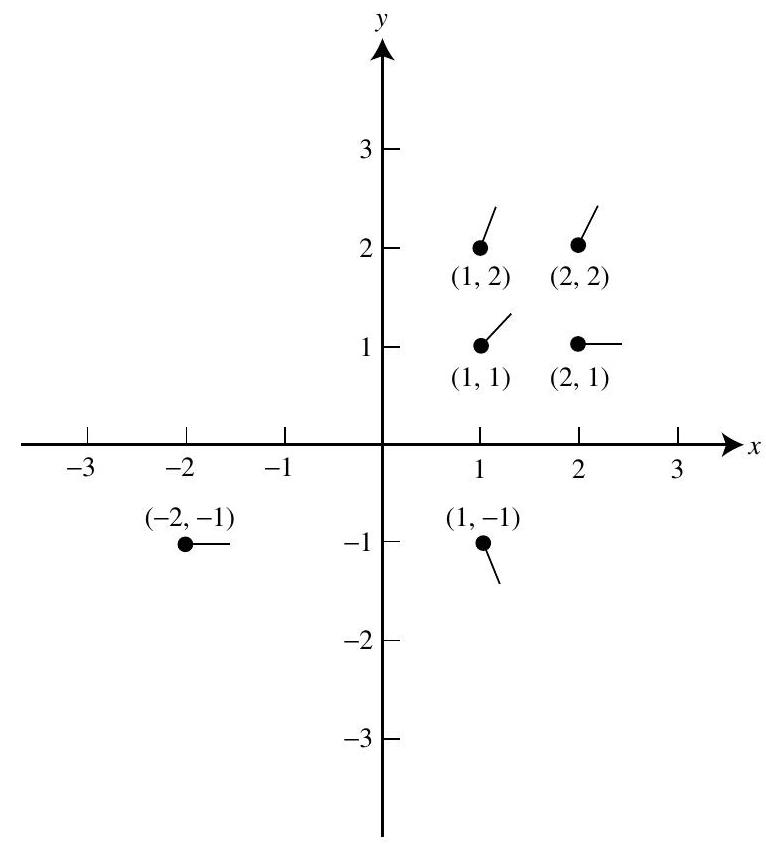
\includegraphics[max width=\textwidth]{2024_04_03_5bb5b4275a64cb9887d1g-177}
\end{center}

Fig. 18-1

\begin{center}
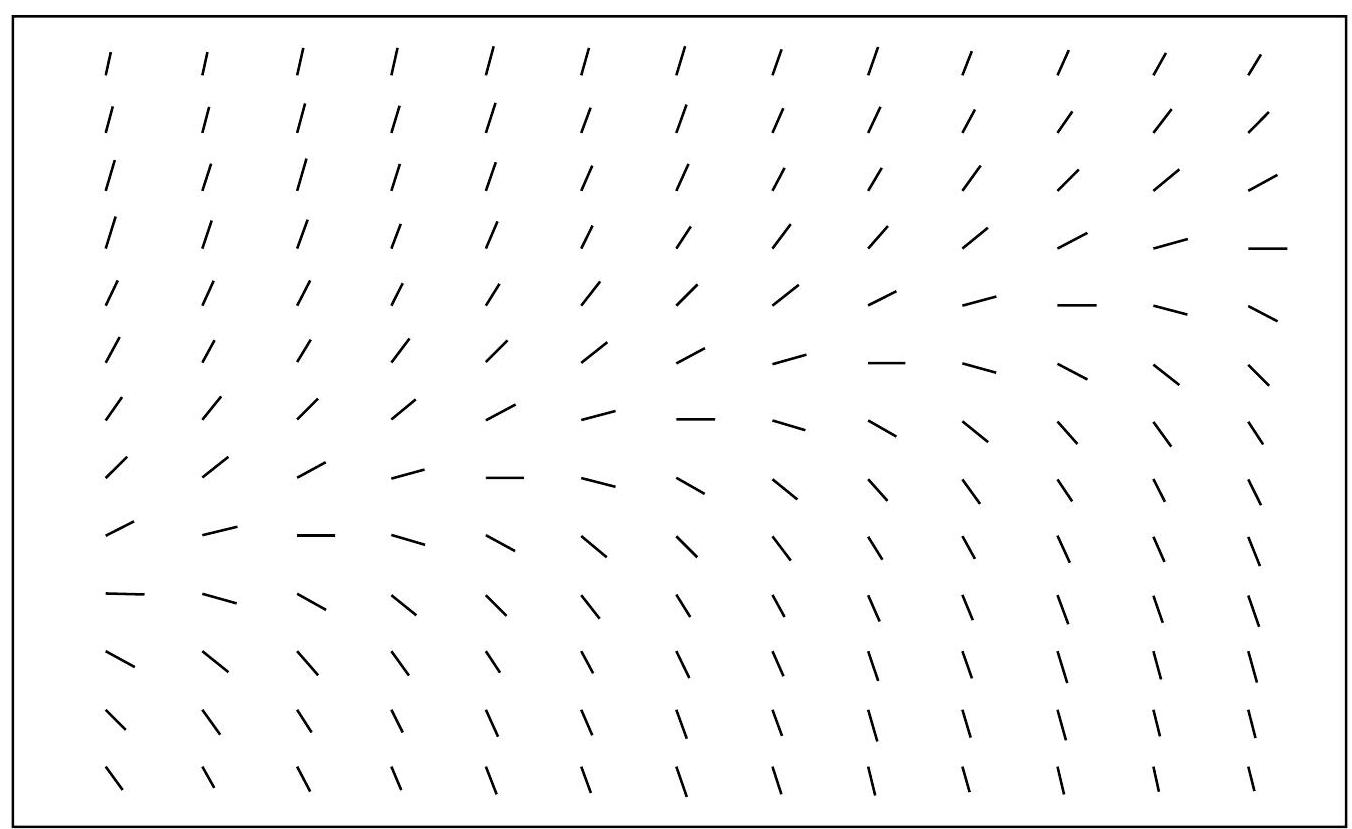
\includegraphics[max width=\textwidth]{2024_04_03_5bb5b4275a64cb9887d1g-177(1)}
\end{center}

Fig. 18-2

18.2. Describe the isoclines associated with the differential equation defined in Problem 18.1.

Isoclines are defined by setting $y^{\prime}=c$, a constant. For the differential equation in Problem 18.1, we obtain

$$
c=2 y-x \quad \text { or } \quad y=\frac{1}{2} x+\frac{1}{2} c
$$

which is the equation for a straight line. Three such isoclines, corresponding to $c=1, c=0$, and $c=-1$, are graphed in Fig. 18-3. On the isocline corresponding to $c=1$, every line element beginning on the isocline will have a slope of unity. On the isocline corresponding to $c=0$, every line element beginning on the isocline will have a slope of zero. On the isocline corresponding to $c=-1$, every line element beginning on the isocline will have a slope of negative one. Some of these line elements are also drawn in Fig. 18-3.

\begin{center}
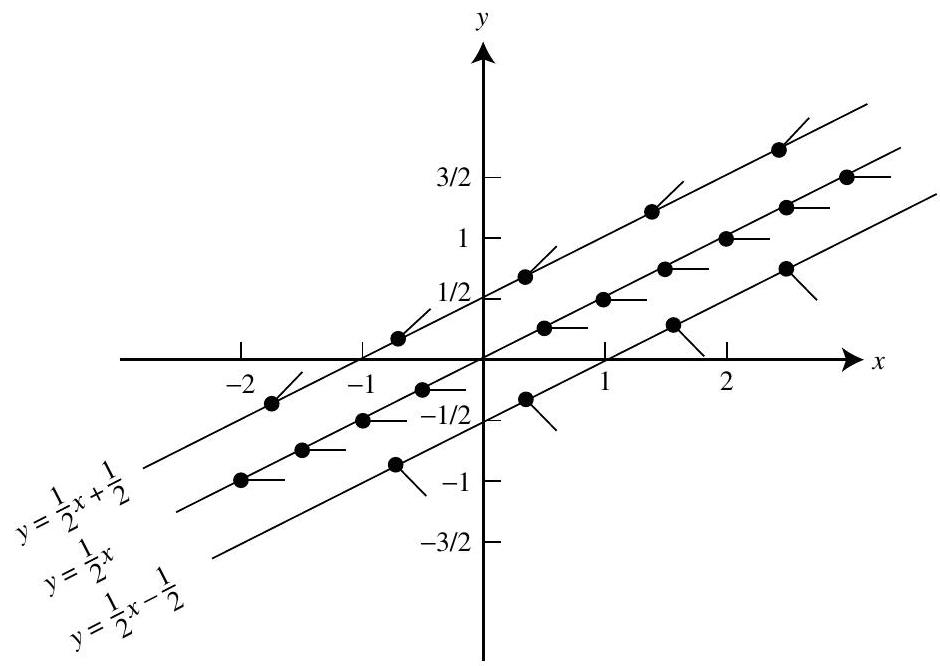
\includegraphics[max width=\textwidth]{2024_04_03_5bb5b4275a64cb9887d1g-178}
\end{center}

Fig. 18-3

18.3. Draw two solution curves to the differential equation given in Problem 18.1.

A direction field for this equation is given by Fig. 18-2. Two solution curves are shown in Fig. 18-4, one that passes through the point $(0,0)$ and a second that passes through the point $(0,2)$. Observe that each solution curve follows the flow of the line elements in the direction field.

18.4. Construct a direction field for the differential equation $y^{\prime}=x^{2}+y^{2}-1$.

Here $f(x, y)=x^{2}+y^{2}-1$.

At $x=0, y=0, f(0,0)=(0)^{2}+(0)^{2}-1=-1$, equivalent to an angle of $-45^{\circ}$.

At $x=1, y=2, f(1,2)=(1)^{2}+(2)^{2}-1=4$, equivalent to an angle of $76.0^{\circ}$.

At $x=-1, y=2, f(-1,2)=(-1)^{2}+(2)^{2}-1=4$, equivalent to an angle of $76.0^{\circ}$.

At $x=0.25, y=0.5, f(0.25,0.5)=(0.25)^{2}+(0.5)^{2}-1=-0.6875$, equivalent to an angle of $-34.5^{\circ}$.

At $x=-0.3, y=-0.1, f(-0.3,-0.1)=(-0.3)^{2}+(-0.1)^{2}-1=-0.9$, equivalent to an angle of $-42.0^{\circ}$.

Continuing in this manner, we generate Fig. 18-5. At each point, we graph a short line segment emanating from the point at the specified angle from the horizontal. To avoid confusion between line elements associated with the differential equation and axis markings, we deleted the axes in Fig. 18-5. The origin is at the center of the graph.

18.5. Describe the isoclines associated with the differential equation defined in Problem 18.4.

Isoclines are defined by setting $y^{\prime}=c$, a constant. For the differential equation in Problem 18.4, we obtain $c=x^{2}+y^{2}-1$ or $x^{2}+y^{2}=c+1$, which is the equation for a circle centered at the origin. Three such isoclines,

\begin{center}
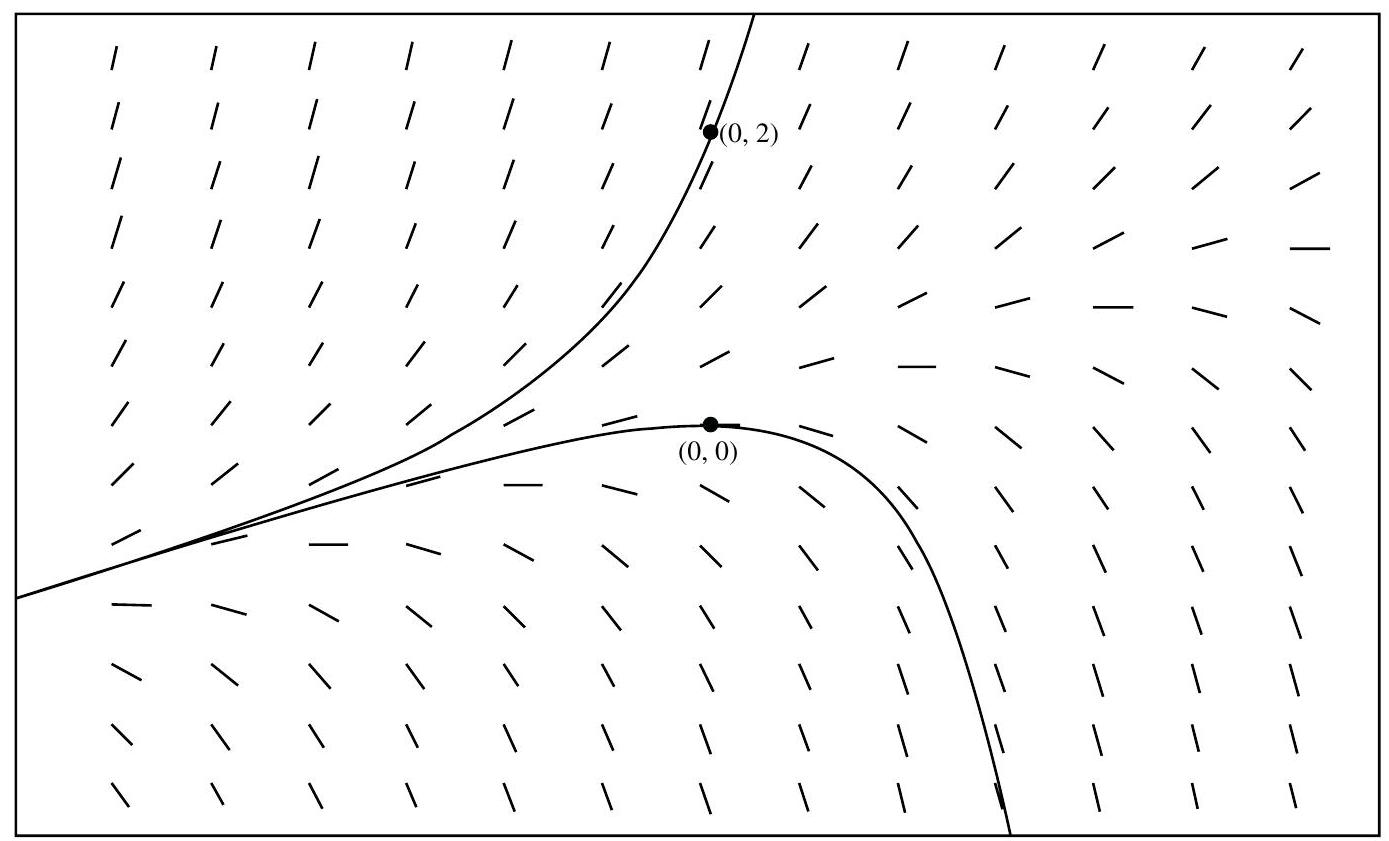
\includegraphics[max width=\textwidth]{2024_04_03_5bb5b4275a64cb9887d1g-179}
\end{center}

Fig. 18-4

\begin{center}
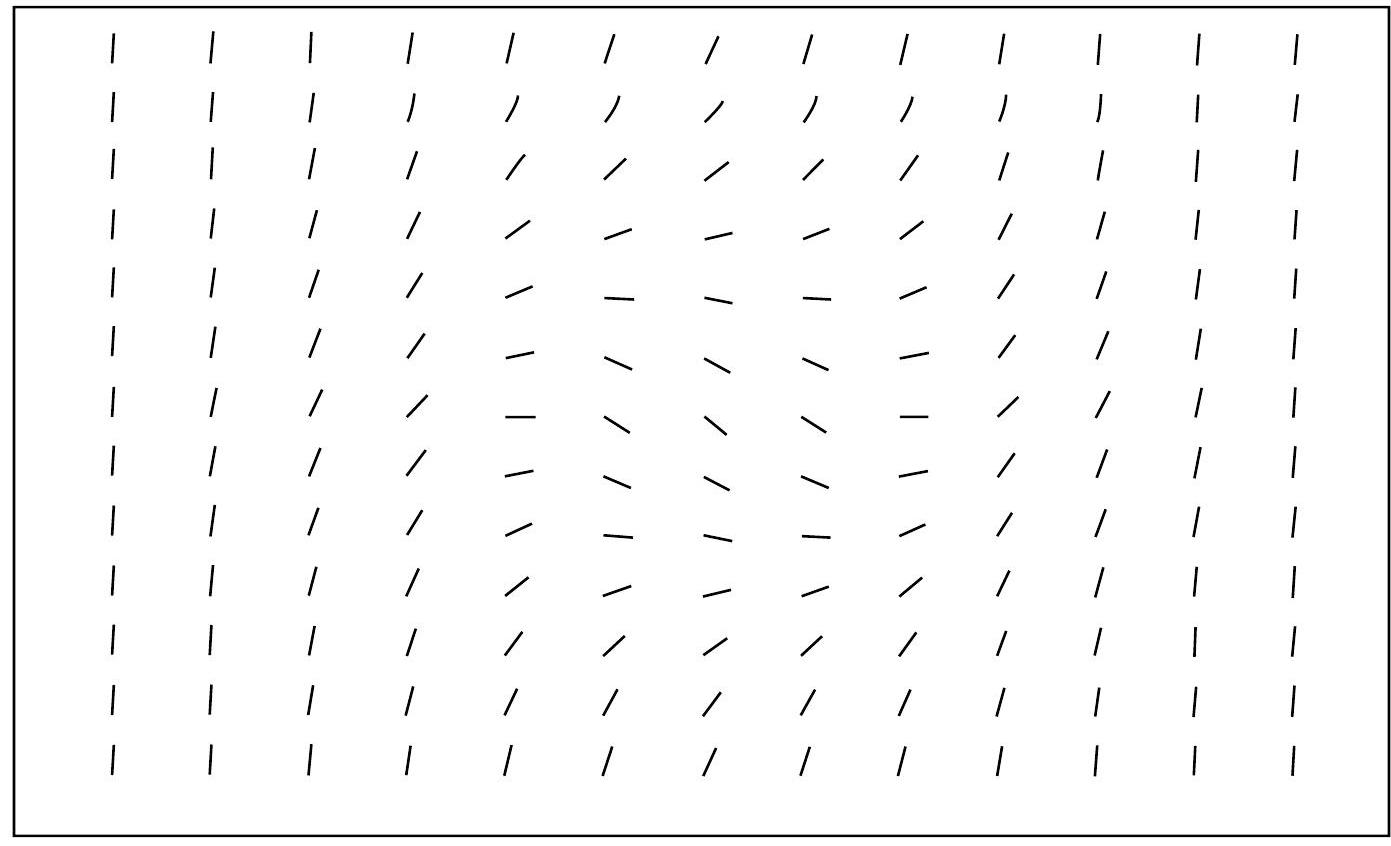
\includegraphics[max width=\textwidth]{2024_04_03_5bb5b4275a64cb9887d1g-179(1)}
\end{center}

Fig. 18-5

corresponding to $c=4, c=1$, and $c=0$, are graphed in Fig. 18-6. On the isocline corresponding to $c=4$, every line element beginning on the isocline will have a slope of four. On the isocline corresponding to $c=1$, every line element beginning on the isocline will have a slope of unity. On the isocline corresponding to $c=0$, every line element beginning on the isocline will have a slope of zero. Some of these line elements are also drawn in Fig. 18-6.

18.6. Draw three solution curves to the differential equation given in Problem 18.4.

A direction field for this equation is given by Fig. 18-5. Three solution curves are shown in Fig. 18-7, the top one passes through $(0,1)$, the middle curve passes through $(0,0)$, and the bottom curve passes through $(0,-1)$. Observe that each solution curve follows the flow of the line elements in the direction field.

\begin{center}
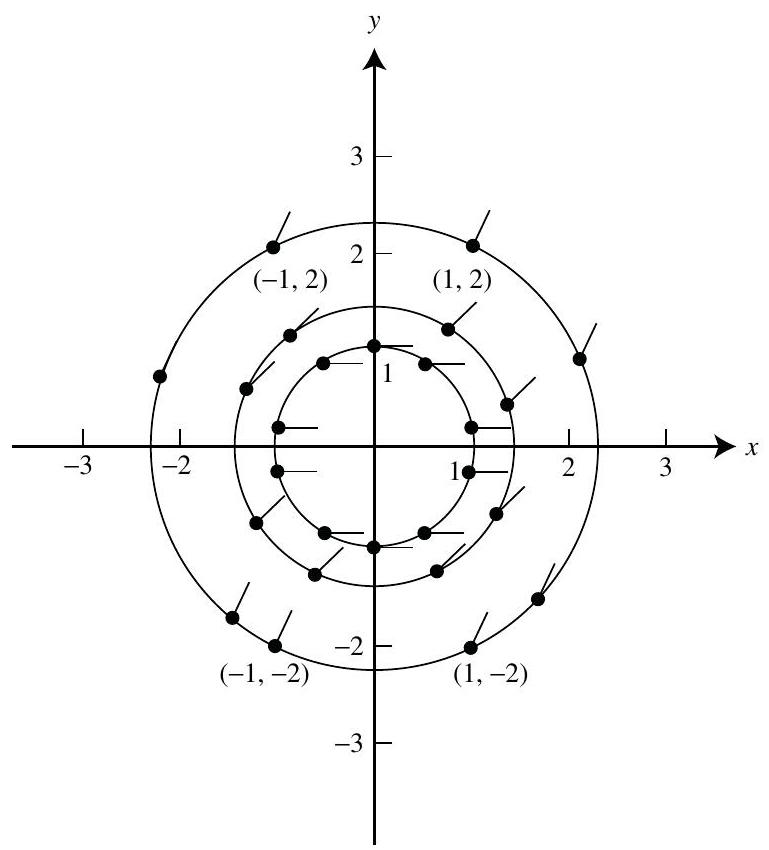
\includegraphics[max width=\textwidth]{2024_04_03_5bb5b4275a64cb9887d1g-180}
\end{center}

Fig. 18-6

\begin{center}
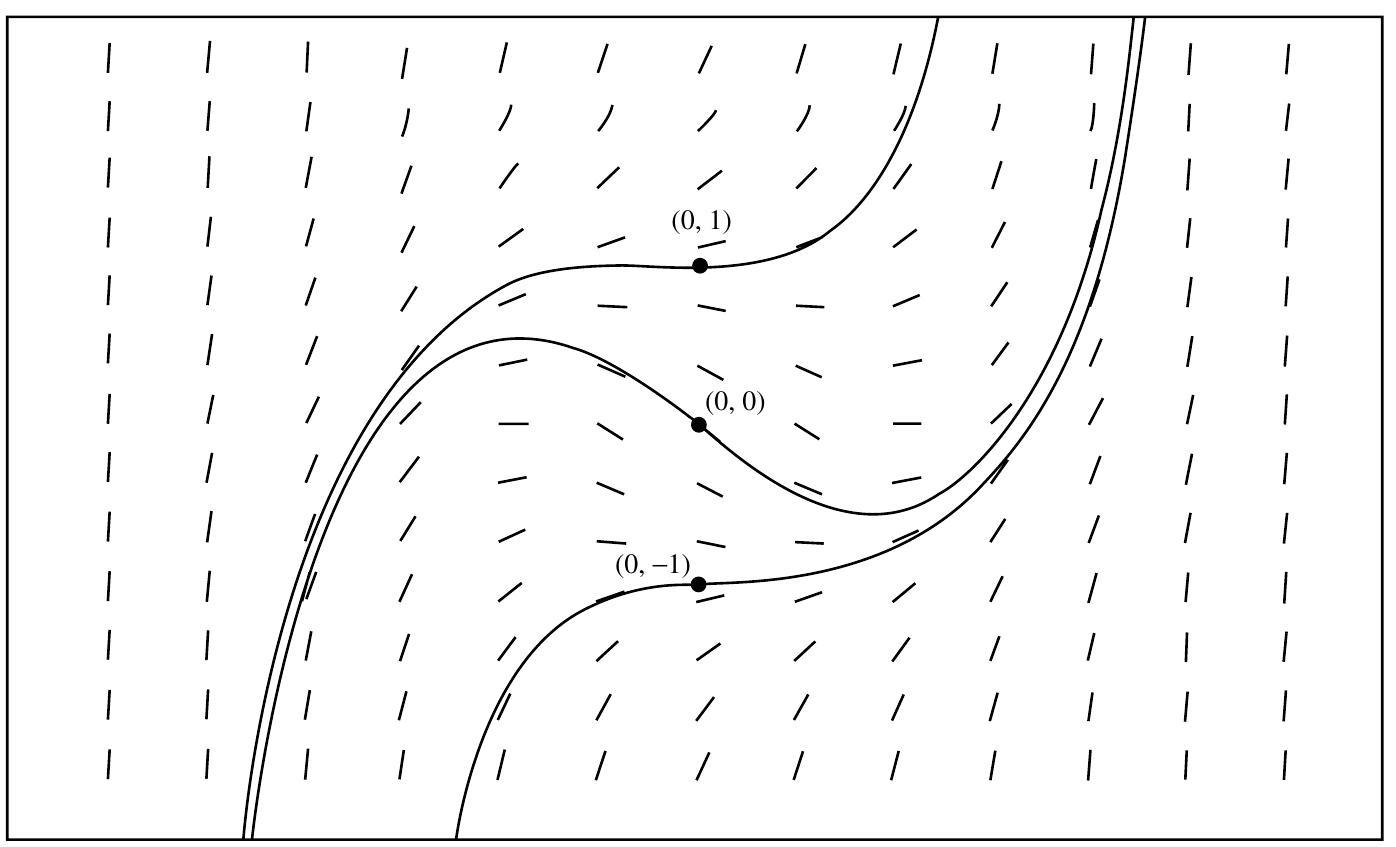
\includegraphics[max width=\textwidth]{2024_04_03_5bb5b4275a64cb9887d1g-180(1)}
\end{center}

Fig. 18-7

\begin{center}
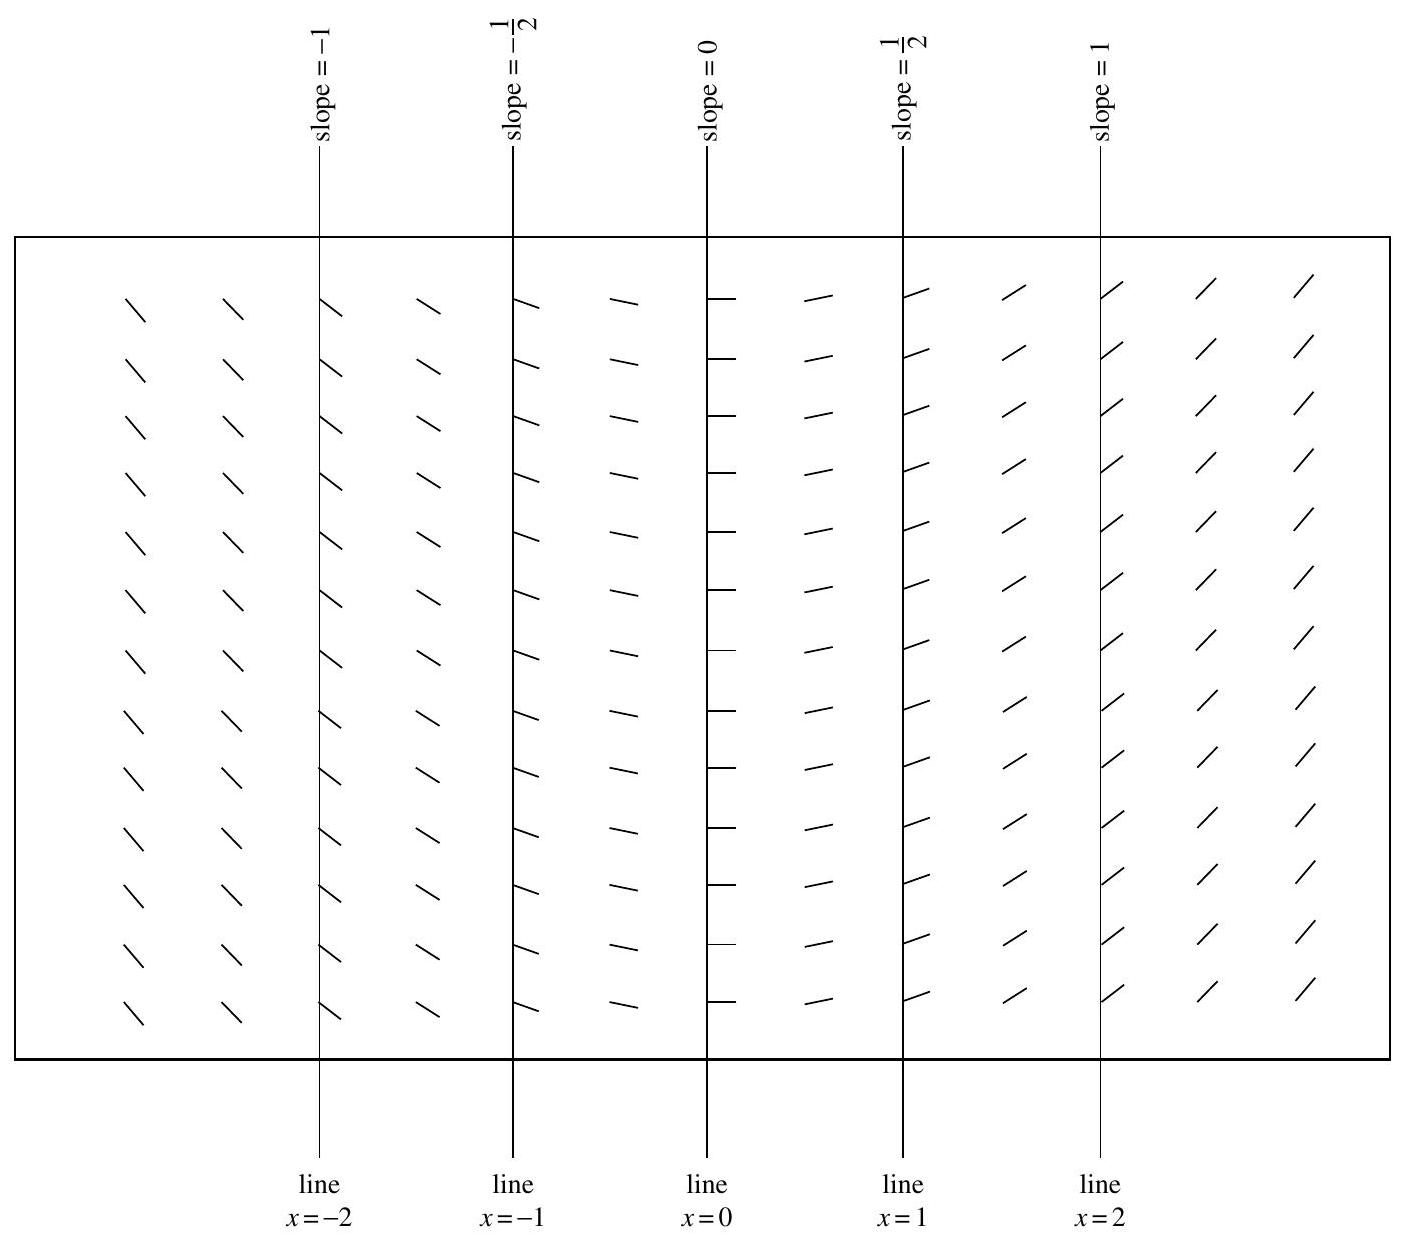
\includegraphics[max width=\textwidth]{2024_04_03_5bb5b4275a64cb9887d1g-181}
\end{center}

Fig. 18-8

18.7. Construct a direction field for the differential equation $y^{\prime}=x / 2$.

Isoclines are defined by setting $y^{\prime}=c$, a constant. Doing so, we obtain $x=2 c$ which is the equation for a vertical straight line. On the isocline $x=2$, corresponding to $c=1$, every line element beginning on the isocline will have a slope of unity. On the isocline $x=-1$, corresponding to $c=-1 / 2$, every line element beginning on the isocline will have a slope of $-\frac{1}{2}$. These and other isoclines with some of their associated line elements are drawn in Fig. 18-8, which is a direction field for the given differential equation.

18.8. Draw four solution curves to the differential equation given in Problem 18.7.

A direction field for this equation is given by Fig. 18-8. Four solution curves are drawn in Fig. 18-9, which from top to bottom pass through the points $(0,1),(0,0),(0,-1)$, and $(0,-2)$, respectively. Note that the differential equation is solved easily by direct integration. Its solution, $y=x^{2} / 4+k$, where $k$ is a constant of integration, is a family of parabolas, one for each value of $k$.

18.9. Draw solution curves to the differential equation $y^{\prime}=5 y(y-1)$.

A direction field for this equation is given by Fig. 18-10. Two isoclines with line elements having zero slopes are the horizontal straight lines $y=0$ and $y=1$. Observe that solution curves have different shapes depending on whether they are above both of these isoclines, between them, or below them. A representative solution curve of each type is drawn in Fig. 18-11(a) through (c).

\begin{center}
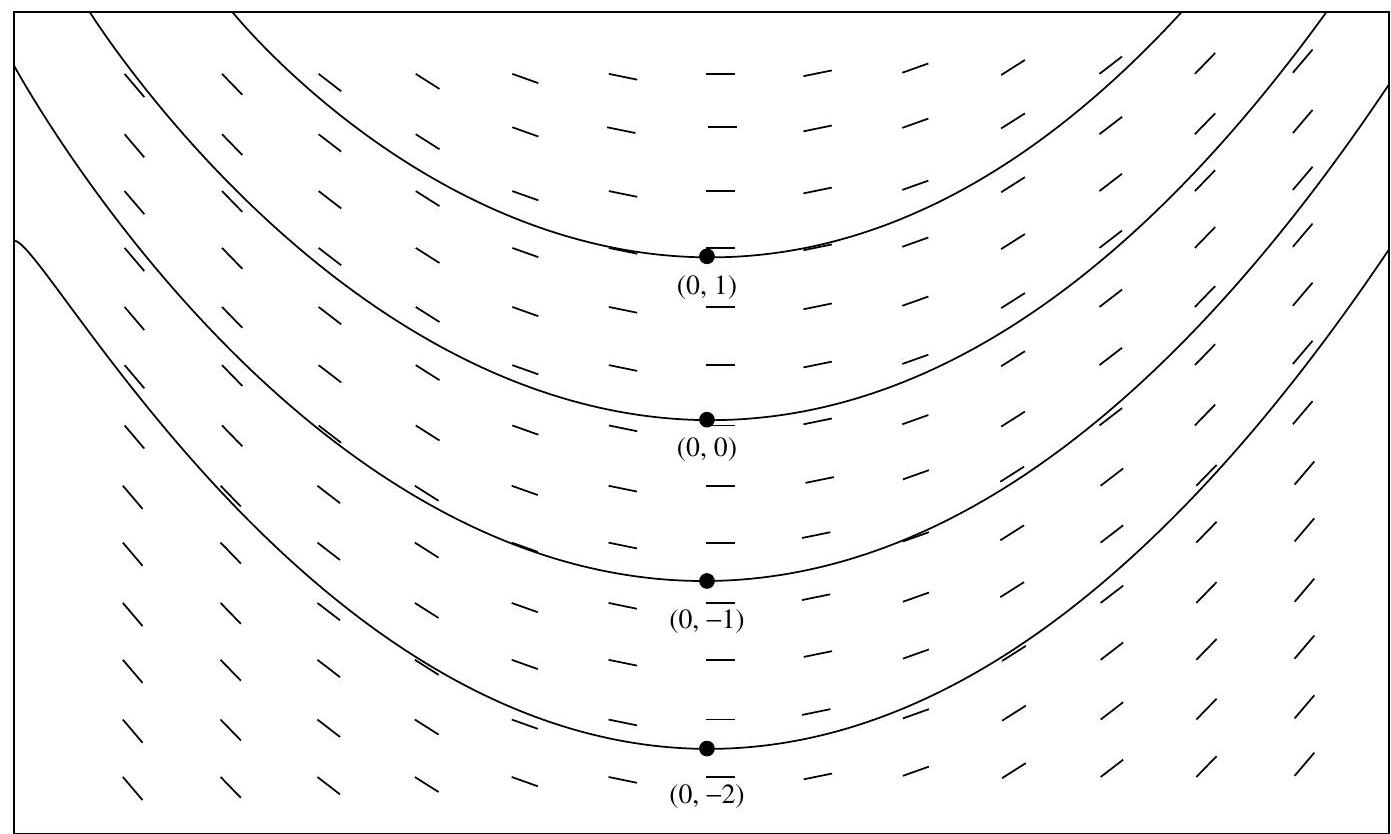
\includegraphics[max width=\textwidth]{2024_04_03_5bb5b4275a64cb9887d1g-182}
\end{center}

Fig. 18-9

\begin{center}
\begin{tabular}{lllllllllllllllllll|}
\hline
 & 1 & 1 & 1 & 1 & 1 & 1 & 1 & 1 & 1 & 1 & 1 & 1 & 1 & 1 & 1 & 1 & 1 & 1 \\
1 & 1 & 1 & 1 & 1 & 1 & 1 & 1 & 1 & 1 & 1 & 1 & 1 & 1 & 1 & 1 & 1 & 1 & 1 \\
1 & 1 & 1 & 1 & 1 & 1 & 1 & 1 & 1 & 1 & 1 & 1 & 1 & 1 & 1 & 1 & 1 & 1 & 1 \\
1 & 1 & 1 & 1 & 1 & 1 & 1 & 1 & 1 & 1 & 1 & 1 & 1 & 1 & 1 & 1 & 1 & 1 & 1 \\
1 & 1 & 1 & 1 & 1 & 1 & 1 & 1 & 1 & 1 & 1 & 1 & 1 & 1 & 1 & 1 & 1 & 1 & 1 \\
- & - & - & - & - & - & - & - & - & - & - & - & - & - & - & - & - & - & - \\
1 & 1 & 1 & 1 & 1 & 1 & 1 & 1 & 1 & 1 & 1 & 1 & 1 & 1 & 1 & 1 & 1 & 1 & 1 \\
1 & 1 & 1 & 1 & 1 & 1 & 1 & 1 & 1 & 1 & 1 & 1 & 1 & 1 & 1 & 1 & 1 & 1 & 1 \\
1 & 1 & 1 & 1 & 1 & 1 & 1 & 1 & 1 & 1 & 1 & 1 & 1 & 1 & 1 & 1 & 1 & 1 & 1 \\
- & - & - & - & - & - & - & - & - & - & - & - & - & - & - & - & - & - & - \\
1 & 1 & 1 & 1 & 1 & 1 & 1 & 1 & 1 & 1 & 1 & 1 & 1 & 1 & 1 & 1 & 1 & 1 & 1 \\
1 & 1 & 1 & 1 & 1 & 1 & 1 & 1 & 1 & 1 & 1 & 1 & 1 & 1 & 1 & 1 & 1 & 1 & 1 \\
1 & 1 & 1 & 1 & 1 & 1 & 1 & 1 & 1 & 1 & 1 & 1 & 1 & 1 & 1 & 1 & 1 & 1 & 1 \\
1 & 1 & 1 & 1 & 1 & 1 & 1 & 1 & 1 & 1 & 1 & 1 & 1 & 1 & 1 & 1 & 1 & 1 & 1 \\
1 & 1 & 1 & 1 & 1 & 1 & 1 & 1 & 1 & 1 & 1 & 1 & 1 & 1 & 1 & 1 & 1 & 1 & 1 \\
1 & 1 & 1 & 1 & 1 & 1 & 1 & 1 & 1 & 1 & 1 & 1 & 1 & 1 & 1 & 1 & 1 & 1 & 1 \\
1 & 1 & 1 & 1 & 1 & 1 & 1 & 1 & 1 & 1 & 1 & 1 & 1 & 1 & 1 & 1 & 1 & 1 & 1 \\
1 & 1 & 1 & 1 & 1 & 1 & 1 & 1 & 1 & 1 & 1 & 1 & 1 & 1 & 1 & 1 & 1 & 1 & 1 \\
1 & 1 & 1 & 1 & 1 & 1 & 1 & 1 & 1 & 1 & 1 & 1 & 1 & 1 & 1 & 1 & 1 & 1 & 1 \\
\hline
\end{tabular}
\end{center}

Fig. 18-10

18.10. Give a geometric derivation of Euler's method.

Assume that $y_{n}=y\left(x_{n}\right)$ has already been computed, so that $y_{n}^{\prime}$ is also known, via Eq. (18.5). Draw a straight line $l(x)$ emanating from $\left(x_{n}, y_{n}\right)$ and having slope $y_{n}^{\prime}$, and use $l(x)$ to approximate $y(x)$ on the interval $\left[x_{n}, x_{n+1}\right]$ (see

Fig. 18-12). The value $l\left(x_{n+1}\right)$ is taken to be $y_{n+1}$. Thus

and

$$
\begin{gathered}
l(x)=\left(y_{n}^{\prime}\right) x+\left[y_{n}-\left(y_{n}^{\prime}\right) x_{n}\right] \\
l\left(x_{n+1}\right)=\left(y_{n}^{\prime}\right) x_{n+1}+\left[y_{n}-\left(y_{n}^{\prime}\right) x_{n}\right] \\
=y_{n}+\left(y_{n}^{\prime}\right)\left(x_{n+1}-x_{n}\right)=y_{n}+h y_{n}^{\prime}
\end{gathered}
$$

Hence, $y_{n+1}=y_{n}+h y_{n}^{\prime}$, which is Euler's method.

18.11. Give an analytic derivation of Euler's method.

Let $Y(x)$ represent the true solution. Then, using the definition of the derivative, we have

$$
Y^{\prime}\left(x_{n}\right)=\lim _{\Delta x \rightarrow 0} \frac{Y\left(x_{n}+\Delta x\right)-Y\left(x_{n}\right)}{\Delta x}
$$

If $\Delta x$ is small, then

$$
Y^{\prime}\left(x_{n}\right) \simeq \frac{Y\left(x_{n}+\Delta x\right)-Y\left(x_{n}\right)}{\Delta x}
$$

Setting $\Delta x=h$ and solving for $Y\left(x_{n}+\Delta x\right)=Y\left(x_{n+1}\right)$, we obtain


\begin{equation*}
Y\left(x_{n+1}\right) \simeq Y\left(x_{n}\right)+h Y^{\prime}\left(x_{n}\right) \tag{1}
\end{equation*}


\begin{center}
\begin{tabular}{|c|c|c|c|c|c|c|c|c|c|c|c|c|c|c|c|c|c|c|}
\hline
1 & 1 & 1 & 1 & 1 & 1 & 1 & 1 & 1 & 1 & 1 & 1 & 1 & 1 & 1 & 1 & 1 & 1 & 1 \\
\hline
1 & 1 & 1 & 1 & 1 & 1 & 1 & 1 & 1 & 11 & 1 & 1 & 1 & 1 & 1 & 1 & 1 & 1 & 1 \\
\hline
1 & 1 & 1 & 1 & 1 & 1 & 1 & 1 & 1 & 11 & 1 & 1 & 1 & 1 & 1 & 1 & 1 & 1 & 1 \\
\hline
1 & $/$ & 1 & 1 & 1 & 1 & / & 1 & I & $l$ & I & / & 1 & I & I & I & I & 1 & 1 \\
\hline
/ & 1 & 1 & 1 & I & 1 & 1 & 1 & 1 & 11 & 1 & / & 1 & 1 & 1 & 1 & I & 1 & 1 \\
\hline
 &  &  &  &  &  &  &  &  & - & - & - & - & - & - & - & - & - & - \\
\hline
$\backslash$ & $\backslash$ & $\backslash$ & $\backslash$ & $\backslash$ & $\backslash$ & $\backslash$ & $\backslash$ & $\backslash$ & $\backslash$ & $\backslash$ & $\backslash$ & $\backslash$ & $\backslash$ & $\backslash$ & $\backslash$ & $\backslash$ & $\backslash$ & $\backslash$ \\
\hline
$\backslash$ & $\backslash$ & $\backslash$ & $\backslash$ & $\backslash$ & $\backslash$ & $\backslash$ & $\backslash$ & $\backslash$ & $\backslash$ & $\backslash$ & $\backslash$ & $\backslash$ & $\backslash$ & $\backslash$ & $\backslash$ & $\backslash$ & $\backslash$ & $\backslash$ \\
\hline
$\backslash$ & $\backslash$ & $\backslash$ & $\backslash$ & $\backslash$ & $\backslash$ & $\backslash$ & $\backslash$ & $\backslash$ & $\backslash$ & $\backslash$ & $\backslash$ & $\backslash$ & $\backslash$ & $\backslash$ & $\backslash$ & $\backslash$ & $\backslash$ & $\backslash$ \\
\hline
- & - & - & - & - & - & - & - & - & - & - & - & - & - & - & - & - & - & - \\
\hline
$\prime$ & $\prime$ & $\prime$ & $\prime$ & $\prime$ & $\prime$ & $\prime$ & $\prime$ & $\prime$ & $\prime$ & $\prime$ & $\prime$ & $\prime$ & $\prime$ & $\prime$ & $\prime$ & $\prime$ & $\prime$ & $\prime$ \\
\hline
1 & 1 & 1 & 1 & 1 & $/$ & $/$ & 1 & I & $/$ & I & 1 & 1 & / & I & / & 1 & I & 1 \\
\hline
1 & 1 & 1 & 1 & 1 & 1 & 1 & 1 & 1 & 1 & 1 & 1 & 1 & 1 & 1 & 1 & 1 & 1 & 1 \\
\hline
1 & 1 & 1 & 1 & 1 & 1 & 1 & 1 & 1 & 1 & 1 & 1 & 1 & 1 & 1 & 1 & 1 & 1 & 1 \\
\hline
1 & 1 & 1 & 1 & 1 & 1 & 1 & 1 & 1 & 1 & 1 & 1 & 1 & 1 & 1 & 1 & 1 & 1 & 1 \\
\hline
I & | & I & I & I & I & I & I & I & I & I & I & I & I & I & I & I & I & I \\
\hline
I & I & I & I & I & I & I & I & I & I & I & I & I & I & I & I & I & I & I \\
\hline
I & | & I & I & I & I & I & I & I & I & I & I & I & I & I & I & I & I & I \\
\hline
I & I & I & I & I & I & I & I & I & I & I & I & I & I & I & I & I & I & I \\
\hline
\end{tabular}
\end{center}

Finally, if we use $y_{n}$ and $y_{n}^{\prime}$ to approximate $Y\left(x_{n}\right)$ and $Y^{\prime}\left(x_{n}\right)$, respectively, the right side of (1) can be used to approximate $Y\left(x_{n+1}\right)$. Thus,

which is Euler's method.

$$
y_{n+1}=y_{n}+h y_{n}^{\prime}
$$

(a)

\begin{center}
\begin{tabular}{|llllllllllllllllllll}
\hline
1 & 1 & 1 & 1 & 1 & 1 & 1 & 1 & 1 & 1 & 1 & 1 & 1 & 1 & 1 & 1 & 1 & 1 & 1 \\
1 & 1 & 1 & 1 & 1 & 1 & 1 & 1 & 1 & 1 & 1 & 1 & 1 & 1 & 1 & 1 & 1 & 1 & 1 \\
1 & 1 & 1 & 1 & 1 & 1 & 1 & 1 & 1 & 1 & 1 & 1 & 1 & 1 & 1 & 1 & 1 & 1 & 1 \\
1 & 1 & 1 & 1 & 1 & 1 & 1 & 1 & 1 & 1 & 1 & 1 & 1 & 1 & 1 & 1 & 1 & 1 & 1 \\
1 & 1 & 1 & 1 & 1 & 1 & 1 & 1 & 1 & 1 & 1 & 1 & 1 & 1 & 1 & 1 & 1 & 1 & 1 \\
\hline
1 & 1 & 1 & 1 & 1 & 1 & 1 & 1 & 1 & 1 & 1 & 1 & 1 & 1 & 1 & 1 & 1 & 1 & 1 \\
1 & 1 & 1 & 1 & 1 & 1 & 1 & 1 & 1 &  & 1 & 1 & 1 & 1 & 1 & 1 & 1 & 1 & 1 \\
1 & 1 & 1 & 1 & 1 & 1 & 1 & 1 & 1 & 1 & 1 & 1 & 1 & 1 & 1 & 1 & 1 & 1 & 1 \\
- & - & - & - & - & - & - & - & - & - & - & 1 & 1 & 1 & 1 & 1 & 1 & 1 & 1 \\
1 & 1 & 1 & 1 & 1 & 1 & 1 & 1 & 1 & 1 & 1 & 1 & 1 & 1 & 1 & 1 & 1 & 1 & 1 \\
1 & 1 & 1 & 1 & 1 & 1 & 1 & 1 & 1 & 1 & 1 & 1 & 1 & 1 & 1 & 1 & 1 & 1 & 1 \\
1 & 1 & 1 & 1 & 1 & 1 & 1 & 1 & 1 & 1 & 1 & 1 & 1 & 1 & 1 & 1 & 1 & 1 & 1 \\
1 & 1 & 1 & 1 & 1 & 1 & 1 & 1 & 1 & 1 & 1 & 1 & 1 & 1 & 1 & 1 &  &  &  \\
1 & 1 & 1 & 1 & 1 & 1 & 1 & 1 & 1 & 1 & 1 & 1 & 1 & 1 & 1 & 1 & 1 & 1 & 1 \\
1 & 1 & 1 & 1 & 1 & 1 & 1 & 1 & 1 & 1 & 1 & 1 & 1 & 1 & 1 & 1 & 1 & 1 & 1 \\
1 & 1 & 1 & 1 & 1 & 1 & 1 & 1 & 1 & 1 & 1 & 1 & 1 & 1 & 1 & 1 & 1 & 1 & 1 \\
1 & 1 & 1 & 1 & 1 & 1 & 1 & 1 & 1 & 1 & 1 & 1 & 1 & 1 & 1 & 1 & 1 & 1 & 1 \\
1 & 1 & 1 & 1 & 1 & 1 & 1 & 1 & 1 & 1 & 1 & 1 & 1 & 1 & 1 & 1 & 1 & 1 & 1 \\
\hline
\end{tabular}
\end{center}

(b)

\begin{center}
\begin{tabular}{|lllllllllllllllllll}
\hline
1 & 1 & 1 & 1 & 1 & 1 & 1 & 1 & 1 & 1 & 1 & 1 & 1 & 1 & 1 & 1 & 1 & 1 & 1 \\
1 & 1 & 1 & 1 & 1 & 1 & 1 & 1 & 1 & 1 & 1 & 1 & 1 & 1 & 1 & 1 & 1 & 1 & 1 \\
1 & 1 & 1 & 1 & 1 & 1 & 1 & 1 & 1 & 1 & 1 & 1 & 1 & 1 & 1 & 1 & 1 & 1 & 1 \\
1 & 1 & 1 & 1 & 1 & 1 & 1 & 1 & 1 & 1 & 1 & 1 & 1 & 1 & 1 & 1 & 1 & 1 & 1 \\
1 & 1 & 1 & 1 & 1 & 1 & 1 & 1 & 1 & 1 & 1 & 1 & 1 & 1 & 1 & 1 & 1 & 1 & 1 \\
- & - & - & - & - & - & - & - & - & - & - & - & - & - & - & - & - & - & - \\
1 & 1 & 1 & 1 & 1 & 1 & 1 & 1 & 1 & 1 & 1 & 1 & 1 & 1 & 1 & 1 & 1 & 1 & 1 \\
1 & 1 & 1 & 1 & 1 & 1 & 1 & 1 & 1 & 1 & 1 & 1 & 1 & 1 & 1 & 1 & 1 & 1 & 1 \\
1 & 1 & 1 & 1 & 1 & 1 & 1 & 1 & 1 & 1 & 1 & 1 & 1 & 1 & 1 & 1 & 1 & 1 & 1 \\
- & - & - & - & - & - & - & - & - & - & - & 1 & 1 & 1 & 1 & 1 & 1 & 1 & 1 \\
1 & 1 & 1 & 1 & 1 & 1 & 1 & 1 & 1 & 1 & 1 & 1 & 1 & 1 & 1 & 1 & 1 & 1 & 1 \\
1 & 1 & 1 & 1 & 1 & 1 & 1 & 1 & 1 & 1 & 1 & 1 & 1 & 1 & 1 & 1 & 1 & 1 & 1 \\
1 & 1 & 1 & 1 & 1 & 1 & 1 & 1 & 1 & 1 & 1 & 1 & 1 & 1 &  &  &  &  &  \\
1 & 1 & 1 & 1 & 1 & 1 & 1 & 1 & 1 & 1 & 1 & 1 & 1 & 1 & 1 & 1 & 1 & 1 & 1 \\
1 & 1 & 1 & 1 & 1 & 1 & 1 & 1 & 1 & 1 & 1 & 1 & 1 & 1 & 1 & 1 & 1 & 1 &  \\
1 & 1 & 1 & 1 & 1 & 1 & 1 & 1 & 1 & 1 & 1 & 1 & 1 & 1 & 1 & 1 & 1 & 1 &  \\
1 & 1 & 1 & 1 & 1 & 1 & 1 & 1 & 1 & 1 & 1 & 1 & 1 & 1 & 1 & 1 & 1 & 1 &  \\
1 & 1 & 1 & 1 & 1 & 1 & 1 & 1 & 1 & 1 & 1 & 1 & 1 & 1 & 1 & 1 & 1 & 1 &  \\
1 & 1 & 1 & 1 & 1 & 1 & 1 & 1 & 1 & 1 & 1 & 1 & 1 & 1 & 1 & 1 & 1 & 1 &  \\
\hline
\end{tabular}
\end{center}

(c)

Fig. 18-11 (cont.)

18.12. Find $y(1)$ for $y^{\prime}=y-x ; y(0)=2$, using Euler's method with $h=\frac{1}{4}$.

For this problem, $x_{0}=0, y_{0}=2$, and $f(x, y)=y-x$; so Eq. (18.5) becomes $y_{n}^{\prime}=y_{n}-x_{n}$. Because $h=\frac{1}{4}$,

$$
x_{1}=x_{0}+h=\frac{1}{4} \quad x_{2}=x_{1}+h=\frac{1}{2} \quad x_{3}=x_{2}+h=\frac{3}{4} \quad x_{4}=x_{3}+h=1
$$

Using Eq. (18.4) with $n=0,1,2,3$ successively, we now compute the corresponding $y$-values.

\begin{center}
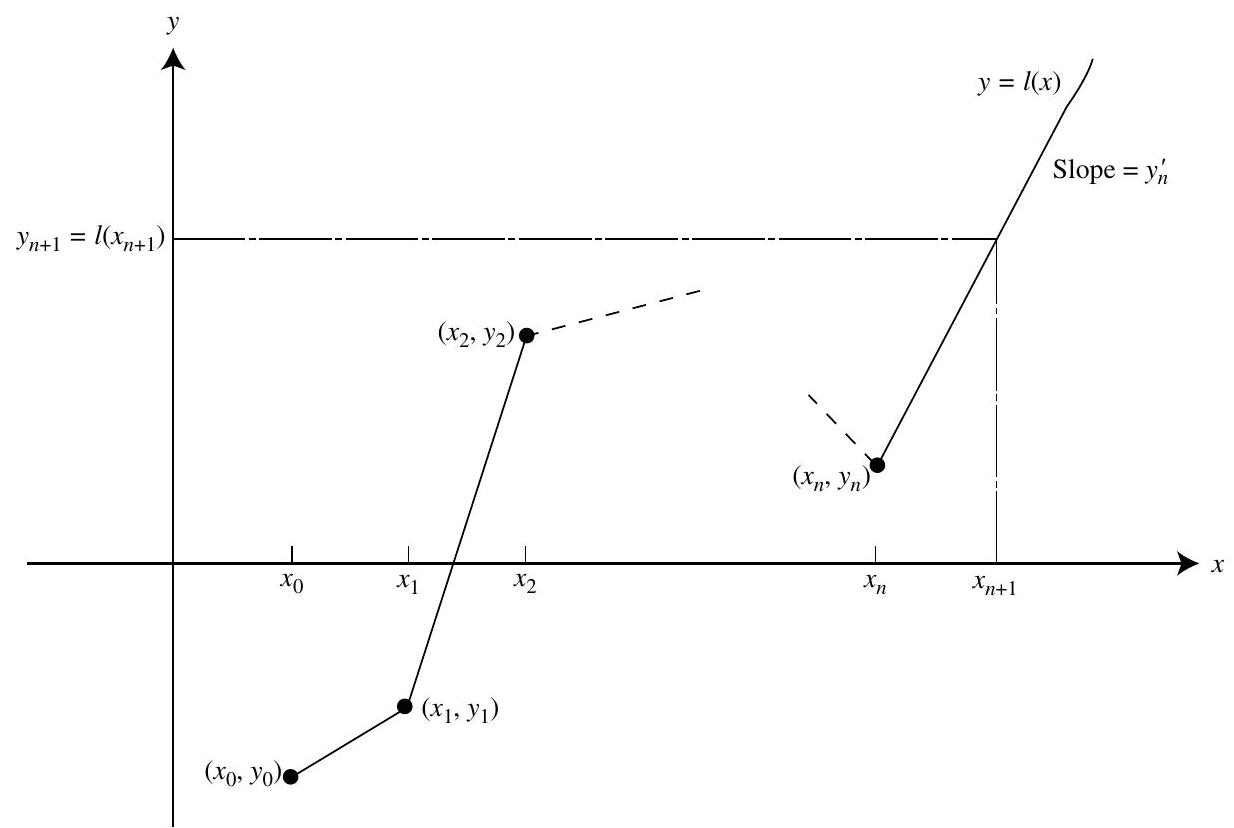
\includegraphics[max width=\textwidth]{2024_04_03_5bb5b4275a64cb9887d1g-185}
\end{center}

Fig. 18-12

$\mathbf{n}=\mathbf{0}: \quad y_{1}=y_{0}+h y_{0}^{\prime}$

But $y_{0}^{\prime}=f\left(x_{0}, y_{0}\right)=y_{0}-x_{0}=2-0=2$

Hence, $y_{1}=2+\frac{1}{4}(2)=\frac{5}{2}$

$\mathbf{n}=\mathbf{1}: \quad y_{2}=y_{1}+h y_{1}^{\prime}$

But $y_{1}^{\prime}=f\left(x_{1}, y_{1}\right)=y_{1}-x_{1}=\frac{5}{2}-\frac{1}{4}=\frac{9}{4}$

Hence, $y_{2}=\frac{5}{2}+\frac{1}{4}\left(\frac{9}{4}\right)=\frac{49}{16}$

$\mathbf{n}=\mathbf{2}: \quad y_{3}=y_{2}+h y_{2}^{\prime}$

But $y_{2}^{\prime}=f\left(x_{2}, y_{2}\right)=y_{2}-x_{2}=\frac{49}{16}-\frac{1}{2}=\frac{41}{16}$

Hence, $y_{3}=\frac{49}{16}+\frac{1}{4}\left(\frac{41}{16}\right)=\frac{237}{64}$

$\mathbf{n}=\mathbf{3}: \quad y_{4}=y_{3}+h y_{3}^{\prime}$

But $y_{3}^{\prime}=f\left(x_{3}, y_{3}\right)=y_{3}-x_{3}=\frac{237}{64}-\frac{3}{4}=\frac{189}{64}$

Hence, $y_{4}=\frac{237}{64}+\frac{1}{4}\left(\frac{189}{64}\right)=\frac{1137}{256}$

Thus,

$$
y(1)=y_{4}=\frac{1137}{256}=4.441
$$

Note that the true solution is $Y(x)=e^{x}+x+1$, so that $Y(1)=4.718$. If we plot $\left(x_{n}, y_{n}\right)$ for $n=0,1,2,3$, and 4 , and then connect successive points with straight line segments, as done in Fig. 18-13, we have an approximation to the solution curve on $[0,1]$ for this initial-value problem.

18.13. Solve Problem 18.12 with $h=0.1$.

With $h=0.1, y(1)=y_{10}$. As before, $y_{n}^{\prime}=y_{n}-x_{n}$. Then, using Eq. (18.4) with $n=0,1, \ldots, 9$ successively, we obtain

$$
\begin{array}{ll}
\mathbf{n = 0}: & x_{0}=0, \quad y_{0}=2, \quad y_{0}^{\prime}=y_{0}-x_{0}=2-0=2 \\
& y_{1}=y_{0}+h y_{0}^{\prime}=2+(0.1)(2)=2.2 \\
\mathbf{n = 1}: & x_{1}=0.1, \quad y_{1}=2.2, \quad y_{1}^{\prime}=y_{1}-x_{1}=2.2-0.1=2.1 \\
& y_{2}=y_{1}+h y_{1}^{\prime}=2.2+(0.1)(2.1)=2.41 \\
\mathbf{n = \mathbf { 2 }}: & x_{2}=0.2, \quad y_{2}=2.41, \quad y_{2}^{\prime}=y_{2}-x_{2}=2.41-0.2=2.21 \\
& y_{3}=y_{2}+h y_{2}^{\prime}=2.41+(0.1)(2.21)=2.631 \\
\mathbf{n = 3}: & x_{3}=0.3, \quad y_{3}=2.631, \quad y_{3}^{\prime}=y_{3}-x_{3}=2.631-0.3=2.331 \\
& y_{4}=y_{3}+h y_{3}^{\prime}=2.631+(0.1)(2.331)=2.864 \\
\mathbf{n = 4 :} & x_{4}=0.4, \quad y_{4}=2.864, \quad y_{4}^{\prime}=y_{4}-x_{4}=2.864-0.4=2.464 \\
& y_{5}=y_{4}+h y_{4}^{\prime}=2.864+(0.1)(2.464)=3.110 \\
\mathbf{n = 5 :} & x_{5}=0.5, \quad y_{5}=3.110, \quad y_{5}^{\prime}=y_{5}-x_{5}=3.110-0.5=2.610 \\
& y_{6}=y_{5}+h y_{5}^{\prime}=3.110+(0.1)(2.610)=3.371 \\
\mathbf{n = 6}: & x_{6}=0.6, \quad y_{6}=3.371, \quad y_{6}^{\prime}=y_{6}-x_{6}=3.371-0.6=2.771 \\
& y_{7}=y_{6}+h y_{6}^{\prime}=3.371+(0.1)(2.771)=3.648 \\
\mathbf{n = 7 :} & x_{7}=0.7, \quad y_{7}=3.648, \quad y_{7}^{\prime}=y_{7}=x_{7}=3.648-0.7=2.948 \\
& y_{8}=y_{7}+h y_{7}^{\prime}=3.648+(0.1)(2.948)=3.943 \\
\mathbf{n = 8}: & x_{8}=0.8, \quad y_{8}=3.943, \quad y_{8}^{\prime}=y_{8}-x_{8}=3.943-0.8=3.143 \\
& y_{9}=y_{8}+h y_{8}^{\prime}=3.943+(0.1)(3.143)=4.257 \\
\mathbf{n = 9 :} & x_{9}=0.9, \quad y_{9}=4.257, \quad y_{9}^{\prime}=y_{9}-x_{9}=4.257-0.9=3.357 \\
& y_{10}=y_{9}+h y_{9}^{\prime}=4.257+(0.1)(3.357)=4.593
\end{array}
$$

\begin{center}
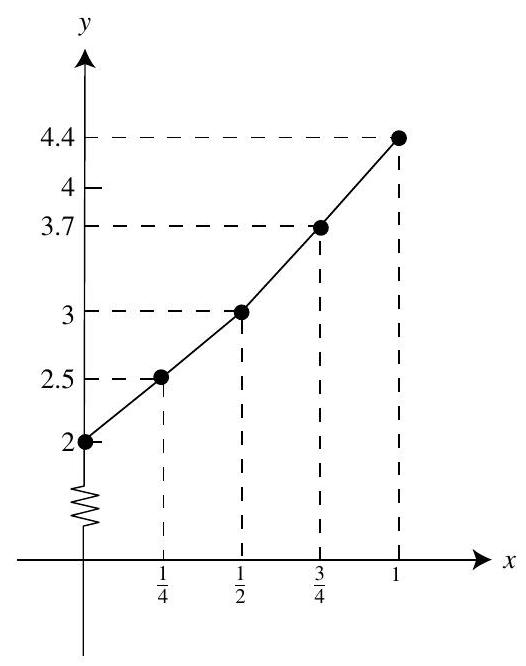
\includegraphics[max width=\textwidth]{2024_04_03_5bb5b4275a64cb9887d1g-186}
\end{center}

Fig. 18-13

The above results are displayed in Table 18-1: For comparison, Table 18-1 also contains results for $h=0.05$, $h=0.01$, and $h=0.005$, with all computations rounded to four decimal places. Note that more accurate results are obtained when smaller values of $h$ are used.

If we plot $\left(x_{n}, y_{n}\right)$ for integer values of $n$ between 0 and 10, inclusively, and then connect successive points with straight line segments, we would generate a graph almost indistinguishable from Fig. 18-13, because graphical accuracy with the chosen scales on the axes is limited to one decimal place.

18.14. Find $y(0.5)$ for $y^{\prime}=y ; y(0)=1$, using Euler's method with $h=0.1$.

For this problem, $f(x, y)=y, x_{0}=0$, and $y_{0}=1$; hence, from Eq. (18.5), $y_{n}^{\prime}=f\left(x_{n}, y_{n}\right)=y_{n}$. With $h=0.1$, $y(0.5)=y_{5}$. Then, using Eq. (18.4) with $n=0,1,2,3,4$ successively, we obtain

$$
\begin{array}{ll}
\mathbf{n = 0}: & x_{0}=0, \quad y_{0}=1, \quad y_{0}^{\prime}=y_{0}=1 \\
& y_{1}=y_{0}+h y_{0}^{\prime}=1+(0.1)(1)=1.1 \\
\mathbf{n = 1 :} & x_{1}=0.1, \quad y_{1}=1.1, \quad y_{1}^{\prime}=y_{1}=1.1 \\
& y_{2}=y_{1}+h y_{1}^{\prime}=1.1+(0.1)(1.1)=1.21 \\
\mathbf{n = 2}: & x_{2}=0.2, \quad y_{2}=1.21, \quad y_{2}^{\prime}=y_{2}=1.21 \\
& y_{3}=y_{2}+h y_{2}^{\prime}=1.21+(0.1)(1.21)=1.331 \\
\mathbf{n = 3}: & x_{3}=0.3, \quad y_{3}=1.331, \quad y_{3}^{\prime}=y_{3}=1.331 \\
& y_{4}=y_{3}+h y_{3}^{\prime}=1.331+(0.1)(1.331)=1.464 \\
\mathbf{n = 4 :} & x_{4}=0.4, \quad y_{4}=1.464, \quad y_{4}^{\prime}=y_{4}=1.464 \\
& y_{5}=y_{4}+h y_{4}^{\prime}=1.464+(0.1)(1.464)=1.610
\end{array}
$$

\begin{center}
\begin{tabular}{|c|c|c|c|c|c|}
\hline
\multicolumn{5}{|c|}{EULER'S METHOD} &  \\
\hline
\multicolumn{2}{|r|}{Problem:} & \multicolumn{3}{|c|}{$y^{\prime}=y-x ; y(0)=2$} &  \\
\hline
\multirow[t]{2}{*}{$x_{n}$} & \multicolumn{4}{|c|}{$y_{n}$} & \multirow{2}{*}{}\begin{tabular}{c}
True solution \\
$Y(x)=e^{x}+x+1$ \\
\end{tabular} \\
\hline
 & $h=0.1$ & $h=0.05$ & $h=0.01$ & $h=0.005$ &  \\
\hline
0.0 & 2.0000 & 2.0000 & 2.0000 & 2.0000 & 2.0000 \\
\hline
0.1 & 2.2000 & 2.2025 & 2.2046 & 2.2049 & 2.2052 \\
\hline
0.2 & 2.4100 & 2.4155 & 2.4202 & 2.4208 & 2.4214 \\
\hline
0.3 & 2.6310 & 2.6401 & 2.6478 & 2.6489 & 2.6499 \\
\hline
0.4 & 2.8641 & 2.8775 & 2.8889 & 2.8903 & 2.8918 \\
\hline
0.5 & 3.1105 & 3.1289 & 3.1446 & 3.1467 & 3.1487 \\
\hline
0.6 & 3.3716 & 3.3959 & 3.4167 & 3.4194 & 3.4221 \\
\hline
0.7 & 3.6487 & 3.6799 & 3.7068 & 3.7102 & 3.7138 \\
\hline
0.8 & 3.9436 & 3.9829 & 4.0167 & 4.0211 & 4.0255 \\
\hline
0.9 & 4.2579 & 4.3066 & 4.3486 & 4.3541 & 4.3596 \\
\hline
1.0 & 4.5937 & 4.6533 & 4.7048 & 4.7115 & 4.7183 \\
\hline
\end{tabular}
\end{center}

Thus, $y(0.5)=y_{5}=1.610$. Note that since the true solution is $Y(x)=e^{x}, Y(0.5)=e^{0.5}=1.649$.

Table 18-1

18.15. Find $y(1)$ for $y^{\prime}=y ; y(0)=1$, using Euler's method with $h=0.1$.

We proceed exactly as in Problem 18.14, except that we now calculate through $n=9$. The results of these computations are given in Table 18-2. For comparison, Table 18-2 also contains results for $h=0.05, h=0.001$, and $h=0.005$, with all calculations rounded to four decimal places.

18.16. Find $y(1)$ for $y^{\prime}=y^{2}+1 ; y(0)=0$, using Euler's method with $h=0.1$.

Here, $f(x, y)=y^{2}+1, x_{0}=0$, and $y_{0}=0$; hence, from Eq. (18.5), $y_{n}^{\prime}=f\left(x_{n}, y_{n}\right)=\left(y_{n}\right)^{2}+1$. With $h=0.1$, $y(1)=y_{10}$. Then, using Eq. (18.4) with $n=0,1, \ldots, 9$ successively, we obtain

$$
\begin{array}{ll}
\mathbf{n = 0}: & x_{0}=0, \quad y_{0}=0, \quad y_{0}^{\prime}=\left(y_{0}\right)^{2}+1=(0)^{2}+1=1 \\
& y_{1}=y_{0}+h y_{0}^{\prime}=0+(0.1)(1)=0.1 \\
\mathbf{n = 1 :} & x_{1}=0.1, \quad y_{1}=0.1, \quad y_{1}^{\prime}=\left(y_{1}\right)^{2}+1=(0.1)^{2}+1=1.01 \\
& y_{2}=y_{1}+h y_{1}^{\prime}=0.1+(0.1)(1.01)=0.201 \\
\mathbf{n = 2 :} & x_{2}=0.2, \quad y_{2}=0.201 \\
& y_{2}^{\prime}=\left(y_{2}\right)^{2}+1=(0.201)^{2}+1=1.040 \\
& y_{3}=y_{2}+h y_{2}^{\prime}=0.201+(0.1)(1.040)=0.305 \\
\mathbf{n = 3 :} & x_{3}=0.3, \quad y_{3}=0.305 \\
& y_{3}^{\prime}=\left(y_{3}\right)^{2}+1=(0.305)^{2}+1=1.093 \\
& y_{4}=y_{3}+h y_{3}^{\prime}=0.305+(0.1)(1.093)=0.414
\end{array}
$$

\begin{center}
\begin{tabular}{|c|c|c|c|c|c|}
\hline
 & Method: & \multicolumn{4}{|c|}{EULER'S METHOD} \\
\hline
 & Problem: & \multicolumn{4}{|c|}{$y^{\prime}=y ; y(0)=1$} \\
\hline
\multirow[t]{2}{*}{$x_{n}$} & \multicolumn{4}{|c|}{$y_{n}$} & \multirow{2}{*}{}\begin{tabular}{l}
True solution \\
$\qquad Y(x)=e^{x}$ \\
\end{tabular} \\
\hline
 & $h=0.1$ & $h=0.05$ & $h=0.01$ & $h=0.005$ &  \\
\hline
0.0 & 1.0000 & 1.0000 & 1.0000 & 1.0000 & 1.0000 \\
\hline
0.1 & 1.1000 & 1.1025 & 1.1046 & 1.1049 & 1.1052 \\
\hline
0.2 & 1.2100 & 1.2155 & 1.2202 & 1.2208 & 1.2214 \\
\hline
0.3 & 1.3310 & 1.3401 & 1.3478 & 1.3489 & 1.3499 \\
\hline
0.4 & 1.4641 & 1.4775 & 1.4889 & 1.4903 & 1.4918 \\
\hline
0.5 & 1.6105 & 1.6289 & 1.6446 & 1.6467 & 1.6487 \\
\hline
0.6 & 1.7716 & 1.7959 & 1.8167 & 1.8194 & 1.8221 \\
\hline
0.7 & 1.9487 & 1.9799 & 2.0068 & 2.0102 & 2.0138 \\
\hline
0.8 & 2.1436 & 2.1829 & 2.2167 & 2.2211 & 2.2255 \\
\hline
0.9 & 2.3579 & 2.4066 & 2.4486 & 2.4541 & 2.4596 \\
\hline
1.0 & 2.5937 & 2.6533 & 2.7048 & 2.7115 & 2.7183 \\
\hline
\end{tabular}
\end{center}

Table 18-2

Table 18-3

\begin{center}
\begin{tabular}{|c|c|c|c|c|c|}
\hline
 & Method: & \multicolumn{4}{|c|}{EULER'S METHOD} \\
\hline
 & Problem: & \multicolumn{4}{|c|}{$y^{\prime}=y^{2}+1 ; y(0)=0$} \\
\hline
\multirow[t]{2}{*}{$x_{n}$} & \multicolumn{4}{|c|}{$y_{n}$} & \multirow{2}{*}{}\begin{tabular}{r}
True solution \\
$Y(x)=\tan x$ \\
\end{tabular} \\
\hline
 & $h=0.1$ & $h=0.05$ & $h=0.01$ & $h=0.005$ &  \\
\hline
0.0 & 0.0000 & 0.0000 & 0.0000 & 0.0000 & 0.0000 \\
\hline
0.1 & 0.1000 & 0.1001 & 0.1003 & 0.1003 & 0.1003 \\
\hline
0.2 & 0.2010 & 0.2018 & 0.2025 & 0.2026 & 0.2027 \\
\hline
0.3 & 0.3050 & 0.3070 & 0.3088 & 0.3091 & 0.3093 \\
\hline
0.4 & 0.4143 & 0.4183 & 0.4218 & 0.4223 & 0.4228 \\
\hline
0.5 & 0.5315 & 0.5384 & 0.5446 & 0.5455 & 0.5463 \\
\hline
0.6 & 0.6598 & 0.6711 & 0.6814 & 0.6827 & 0.6841 \\
\hline
0.7 & 0.8033 & 0.8212 & 0.8378 & 0.8400 & 0.8423 \\
\hline
0.8 & 0.9678 & 0.9959 & 1.0223 & 1.0260 & 1.0296 \\
\hline
0.9 & 1. 1615 & 1.2055 & 1.2482 & 1.2541 & 1.2602 \\
\hline
1.0 & 1.3964 & 1.4663 & 1.5370 & 1.5470 & 1.5574 \\
\hline
\end{tabular}
\end{center}

$\boldsymbol{n}=\mathbf{4}: \quad x_{4}=0.4, \quad y_{4}=0.414$

$y_{4}^{\prime}=\left(y_{4}\right)^{2}+1=(0.414)^{2}+1=1.171$

$y_{5}=y_{4}+h y_{4}^{\prime}=0.414+(0.1)(1.171)=0.531$

Continuing in this manner, we find that $y_{10}=1.396$.

The calculations are found in Table 18-3. For comparison, Table 18-3 also contains results for $h=0.05$, $h=0.01$, and $h=0.005$, with all computations rounded to four decimal places. The true solution to this problem is $Y(x)=\tan x$, hence $Y(1)=1.557$.

\section*{Supplementary Problems}
Direction fields are provided in Problems 18.17 through 18.22. Sketch some of the solution curves.

18.17. See Fig. 18-14.

18.19. See Fig. 18-16.

18.21. See Fig. 18-18.

18.23. Draw a direction field for the equation $y^{\prime}=x-y+1$.

18.24. Describe the isoclines for the equation in Problem 18.23 .\\
18.18. See Fig. 18-15

18.20. See Fig. 18-17.

18.22. See Fig. 18-19.

\begin{center}
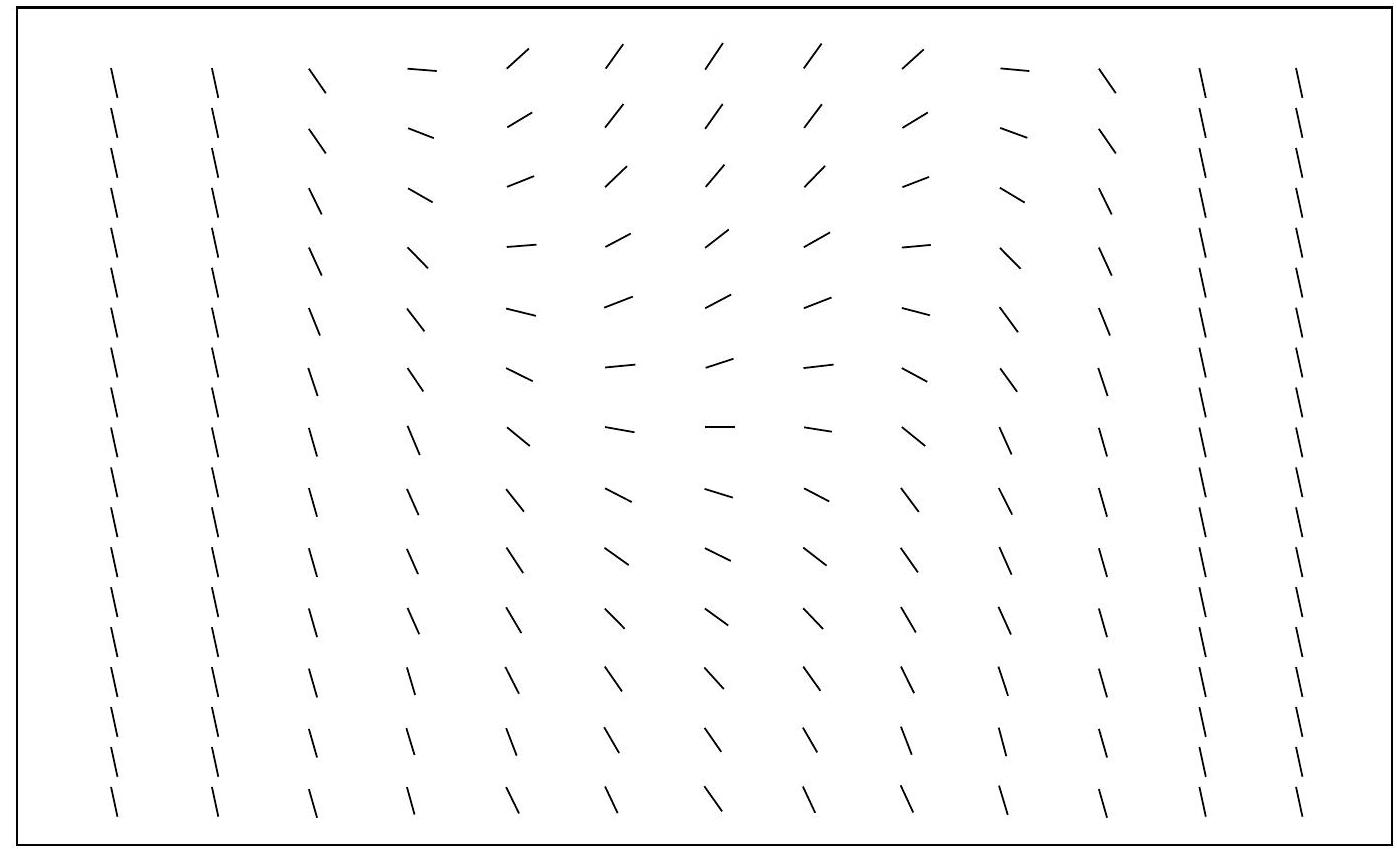
\includegraphics[max width=\textwidth]{2024_04_03_5bb5b4275a64cb9887d1g-190}
\end{center}

Fig. 18-14

\begin{center}
\begin{tabular}{|c|c|c|c|c|c|c|c|c|c|c|c|c|c|c|c|c|c|c|}
\hline
1 & 1 & 1 & 1 & 1 & 1 & $\backslash$ & $\backslash$ & $\backslash$ & - & ' & 1 & 1 & 1 & / & 1 & 1 & 1 & 1 \\
\hline
1 & 1 & 1 & 1 & 1 & $\backslash$ & $\backslash$ & $\backslash$ & $\backslash$ & - & ' & 1 & / & / & / & I & 1 & 1 & 1 \\
\hline
1 & 1 & 1 & 1 & 1 & $\backslash$ & $\backslash$ & $\backslash$ & $\backslash$ & - & ' & I & 1 & / & / & I & 1 & 1 & 1 \\
\hline
1 & 1 & 1 & 1 & 1 & $\backslash$ & $\backslash$ & $\backslash$ & $\backslash$ & - & ' & I & 1 & / & / & I & 1 & 1 & 1 \\
\hline
1 & 1 & 1 & 1 & 1 & $\backslash$ & $\backslash$ & $\backslash$ & $\backslash$ & - & ' & 1 & 1 & 1 & / & 1 & 1 & 1 & 1 \\
\hline
1 & 1 & 1 & 1 & 1 & $\backslash$ & $\backslash$ & $\backslash$ & $\backslash$ & - & ' & 1 & 1 & / & / & 1 & 1 & 1 & 1 \\
\hline
1 & 1 & 1 & 1 & 1 & $\backslash$ & $\backslash$ & $\backslash$ & $\backslash$ & - & ' & / & / & 1 & / & 1 & 1 & 1 & 1 \\
\hline
1 & 1 & 1 & 1 & 1 & 1 & $\backslash$ & $\backslash$ & $\backslash$ & - & ' & 1 & 1 & 1 & / & 1 & 1 & 1 & 1 \\
\hline
1 & 1 & 1 & 1 & $\backslash$ & $\backslash$ & $\backslash$ & $\backslash$ & $\backslash$ & - & ' & I & I & / & / & 1 & 1 & 1 & 1 \\
\hline
1 & 1 & 1 & 1 & 1 & 1 & $\backslash$ & $\backslash$ & $\backslash$ & - & ' & $/$ & 1 & I & / & 1 & 1 & 1 & 1 \\
\hline
1 & 1 & 1 & 1 & 1 & $\backslash$ & $\backslash$ & $\backslash$ & $\backslash$ & - & ' & 1 & 1 & / & / & I & 1 & 1 & 1 \\
\hline
1 & 1 & 1 & 1 & 1 & $\backslash$ & $\backslash$ & $\backslash$ & $\backslash$ & - & ' & 1 & 1 & / & / & 1 & 1 & 1 & 1 \\
\hline
1 & 1 & 1 & 1 & $\backslash$ & $\backslash$ & $\backslash$ & $\backslash$ & $\backslash$ & - & ' & I & / & / & / & 1 & 1 & 1 & 1 \\
\hline
1 & 1 & 1 & 1 & 1 & 1 & $\backslash$ & $\backslash$ & $\backslash$ & - & ' & 1 & 1 & 1 & ' & I & 1 & 1 & 1 \\
\hline
1 & 1 & 1 & 1 & 1 & $\backslash$ & $\backslash$ & $\backslash$ & $\backslash$ & - & ' & 1 & 1 & / & / & 1 & 1 & 1 & 1 \\
\hline
1 & 1 & 1 & 1 & 1 & 1 & $\backslash$ & $\backslash$ & $\backslash$ & - & ' & 1 & 1 & 1 & / & 1 & 1 & 1 & 1 \\
\hline
1 & 1 & 1 & 1 & 1 & 1 & $\backslash$ & $\backslash$ & $\backslash$ & - & ' & 1 & 1 & 1 & $/$ & 1 & 1 & 1 & 1 \\
\hline
1 & 1 & 1 & 1 & 1 & 1 & $\backslash$ & $\backslash$ & $\backslash$ & - & , & 1 & I & / & / & I & 1 & I & 1 \\
\hline
1 & 1 & 1 & 1 & 1 & 1 & $\backslash$ & $\backslash$ & $\backslash$ & - & , & 1 & 1 & / & I & 1 & 1 & 1 & 1 \\
\hline
\end{tabular}
\end{center}

\begin{center}
\begin{tabular}{|c|c|c|c|c|c|c|c|c|c|c|c|c|c|c|c|c|c|c|}
\hline
1 & 1 & $\prime$ & $\prime$ & $\prime$ & $\prime$ & 1 & $\prime$ & $\prime$ & $\prime$ & $\prime$ & $\prime$ & $\prime$ & $\prime$ & $\prime$ & 1 & $\prime$ & 1 & $\prime$ \\
\hline
$\prime$ & ' & ' & , & ' & ' & ' & ' & $\prime$ & $\prime$ & ' & , & ' & $\prime$ & ' & ' & $\prime$ & ' & - \\
\hline
' & - & - & - & - & , & - & - & , & - & , & - & , & , & I & - & - & - & - \\
\hline
- & - & - & - & - & - & - & - & - & - & - & - & - & - & - & - & - & - & - \\
\hline
- & - & - & - & - & - & - & - & - & - & - & - & - & - & - & - & - & - & - \\
\hline
- & - & - & - & - & - & - & - & - & - & - & - & - & - & - & - & - & - & - \\
\hline
- & - & - & - & - & - & - & - & - & - & - & - & - & - & - & - & - & - & - \\
\hline
\textbackslash  & $\backslash$ & $\backslash$ & $\checkmark$ & $\backslash$ & - & - & - & $\backslash$ & $\backslash$ & $\backslash$ & - & $\backslash$ & $\backslash$ & $\backslash$ & $\backslash$ & $\backslash$ & $\backslash$ & $\backslash$ \\
\hline
$\backslash$ & $\backslash$ & $\backslash$ & $\checkmark$ & - & $\backslash$ & $\backslash$ & $\backslash$ & $\backslash$ & $\backslash$ & $\backslash$ & $\backslash$ & $\backslash$ & $\backslash$ & $\backslash$ & $\backslash$ & $\backslash$ & $\backslash$ & \textbackslash  \\
\hline
$\backslash$ & $\backslash$ & $\backslash$ & $\backslash$ & $\backslash$ & $\backslash$ & $\backslash$ & $\backslash$ & $\backslash$ & $\backslash$ & $\backslash$ & $\backslash$ & $\backslash$ & $\backslash$ & $\backslash$ & $\backslash$ & $\backslash$ & $\backslash$ & $\backslash$ \\
\hline
$\backslash$ & $\backslash$ & $\backslash$ & $\backslash$ & $\backslash$ & $\backslash$ & $\backslash$ & $\backslash$ & $\backslash$ & $\backslash$ & $\backslash$ & $\backslash$ & $\backslash$ & $\backslash$ & 1 & $\backslash$ & $\backslash$ & 1 & $\backslash$ \\
\hline
$\backslash$ & $\backslash$ & $\backslash$ & $\backslash$ & $\backslash$ & $\backslash$ & $\backslash$ & $\backslash$ & $\backslash$ & $\backslash$ & $\backslash$ & $\backslash$ & 1 & 1 & $\backslash$ & $\backslash$ & $\backslash$ & $\backslash$ & 1 \\
\hline
$\backslash$ & 1 & $\backslash$ & $\backslash$ & 1 & 1 & $\backslash$ & 1 & $\backslash$ & 1 & 1 & $\backslash$ & 1 & $\backslash$ & 1 & $\backslash$ & 1 & $\backslash$ & 1 \\
\hline
$\backslash$ & $\backslash$ & $\backslash$ & $\backslash$ & $\backslash$ & 1 & $\backslash$ & 1 & $\backslash$ & $\backslash$ & 1 & $\backslash$ & $\backslash$ & $\backslash$ & 1 & $\backslash$ & 1 & $\backslash$ & 1 \\
\hline
$\backslash$ & 1 & 1 & $\backslash$ & $\backslash$ & 1 & 1 & $\backslash$ & $\backslash$ & 1 & 1 & $\backslash$ & $\backslash$ & 1 & $\backslash$ & $\backslash$ & $\backslash$ & 1 & 1 \\
\hline
$\backslash$ & 1 & $\backslash$ & $\backslash$ & 1 & $\backslash$ & 1 & $\backslash$ & $\backslash$ & 1 & 1 & $\backslash$ & $\backslash$ & $\backslash$ & 1 & 1 & $\backslash$ & 1 & 1 \\
\hline
$\backslash$ & $\backslash$ & $\backslash$ & 1 & 1 & $\backslash$ & 1 & $\backslash$ & $\backslash$ & 1 & 1 & 1 & $\backslash$ & $\backslash$ & $\backslash$ & $\backslash$ & 1 & $\backslash$ & 1 \\
\hline
$\backslash$ & 1 & $\backslash$ & 1 & 1 & 1 & 1 & $\backslash$ & 1 & 1 & 1 & $\backslash$ & $\backslash$ & $\backslash$ & $\backslash$ & $\backslash$ & 1 & 1 & 1 \\
\hline
1 & $\backslash$ & 1 & $\backslash$ & 1 & 1 & 1 & $\backslash$ & $\backslash$ & 1 & 1 & $\backslash$ & $\backslash$ & $\backslash$ & $\backslash$ & 1 & 1 & 1 & 1 \\
\hline
\end{tabular}
\end{center}

Fig. 18-16

\begin{center}
\begin{tabular}{llllllllllllllllllll}
\hline
 & 1 & 1 & 1 & 1 & 1 & 1 & 1 & 1 & 1 & 1 & 1 & 1 & - & - & - & 1 & 1 & 1 \\
1 & 1 & 1 & 1 & 1 & 1 & 1 & 1 & 1 & 1 & 1 & 1 & 1 & - & - & - & 1 & 1 & 1 \\
1 & 1 & 1 & 1 & 1 & 1 & 1 & 1 & 1 & 1 & 1 & 1 & 1 & - & 1 & 1 & 1 & 1 & 1 \\
1 & 1 & 1 & 1 & 1 & 1 & 1 & 1 & 1 & 1 & 1 & 1 & - & - & 1 & 1 & 1 & 1 & 1 \\
1 & 1 & 1 & 1 & 1 & 1 & 1 & 1 & 1 & 1 & 1 & - & - & 1 & 1 & 1 & 1 & 1 & 1 \\
1 & 1 & 1 & 1 & 1 & 1 & 1 & 1 & 1 & 1 & - & - & 1 & 1 & 1 & 1 & 1 & 1 & 1 \\
1 & 1 & 1 & 1 & 1 & 1 & 1 & 1 & 1 & 1 & - & 1 & 1 & 1 & 1 & 1 & 1 & 1 & 1 \\
1 & 1 & 1 & 1 & 1 & 1 & 1 & 1 & 1 & - & 1 & 1 & 1 & 1 & 1 & 1 & 1 & 1 & 1 \\
1 & 1 & 1 & 1 & 1 & 1 & 1 & 1 & - & - & 1 & 1 & 1 & 1 & 1 & 1 & 1 & 1 & 1 \\
1 & 1 & 1 & 1 & 1 & 1 & 1 & 1 & - & 1 & 1 & 1 & 1 & 1 & 1 & 1 & 1 & 1 & 1 \\
1 & 1 & 1 & 1 & 1 & 1 & 1 & - & 1 & 1 & 1 & 1 & 1 & 1 & 1 & 1 & 1 & 1 & 1 \\
1 & 1 & 1 & 1 & 1 & 1 & - & - & 1 & 1 & 1 & 1 & 1 & 1 & 1 & 1 & 1 & 1 & 1 \\
1 & 1 & 1 & 1 & 1 & - & - & 1 & 1 & 1 & 1 & 1 & 1 & 1 & 1 & 1 & 1 & 1 & 1 \\
1 & 1 & 1 & 1 & 1 & - & 1 & 1 & 1 & 1 & 1 & 1 & 1 & 1 & 1 & 1 & 1 & 1 & 1 \\
1 & 1 & 1 & - & - & - & 1 & 1 & 1 & 1 & 1 & 1 & 1 & 1 & 1 & 1 & 1 & 1 & 1 \\
1 & 1 & 1 & - & - & 1 & 1 & 1 & 1 & 1 & 1 & 1 & 1 & 1 & 1 & 1 & 1 & 1 & 1 \\
1 & 1 & 1 & - & 1 & 1 & 1 & 1 & 1 & 1 & 1 & 1 & 1 & 1 & 1 & 1 & 1 & 1 & 1 \\
1 & 1 & - & - & 1 & 1 & 1 & 1 & 1 & 1 & 1 & 1 & 1 & 1 & 1 & 1 & 1 & 1 & 1 \\
1 & - & - & 1 & 1 & 1 & 1 & 1 & 1 & 1 & 1 & 1 & 1 & 1 & 1 & 1 & 1 & 1 & 1 \\
\hline
\end{tabular}
\end{center}

$$
\begin{array}{lllllllllllllllllll}
1 & 1 & 1 & 1 & 1 & 1 & 1 & 1 & 1 & 1 & 1 & 1 & 1 & 1 & 1 & 1 & 1 & 1 & 1 \\
1 & 1 & 1 & 1 & 1 & 1 & 1 & 1 & 1 & 1 & 1 & 1 & 1 & 1 & 1 & 1 & 1 & 1 & 1 \\
1 & 1 & 1 & 1 & 1 & 1 & 1 & 1 & 1 & 1 & 1 & 1 & 1 & 1 & 1 & 1 & 1 & 1 & 1 \\
1 & 1 & 1 & 1 & 1 & 1 & 1 & 1 & 1 & 1 & 1 & 1 & 1 & 1 & 1 & 1 & 1 & 1 & 1 \\
1 & 1 & 1 & 1 & 1 & 1 & 1 & 1 & 1 & 1 & 1 & 1 & 1 & 1 & 1 & 1 & 1 & 1 & 1 \\
1 & 1 & 1 & 1 & 1 & 1 & 1 & 1 & 1 & 1 & 1 & 1 & 1 & 1 & 1 & 1 & 1 & 1 & 1 \\
1 & 1 & - & 1 & 1 & 1 & 1 & 1 & 1 & 1 & 1 & 1 & 1 & 1 & 1 & 1 & 1 & 1 & 1 \\
1 & 1 & - & - & 1 & 1 & 1 & 1 & 1 & 1 & 1 & - & - & 1 & 1 & 1 & 1 & 1 & 1 \\
1 & - & - & - & - & 1 & 1 & 1 & 1 & - & - & - & - & - & 1 & 1 & 1 & 1 & - \\
- & - & 1 & 1 & - & - & 1 & 1 & 1 & - & - & 1 & 1 & - & - & 1 & 1 & 1 & - \\
- & 1 & 1 & 1 & 1 & - & - & - & - & - & 1 & 1 & 1 & 1 & - & 1 & 1 & - & - \\
1 & 1 & 1 & 1 & 1 & - & - & - & - & 1 & 1 & 1 & 1 & 1 & - & - & - & - & 1 \\
1 & 1 & 1 & 1 & 1 & 1 & -1 & - & 1 & 1 & 1 & 1 & 1 & 1 & 1 & - & - & 1 & 1 \\
1 & 1 & 1 & 1 & 1 & 1 & 1 & 1 & 1 & 1 & 1 & 1 & 1 & 1 & 1 & 1 & 1 & 1 & 1 \\
1 & 1 & 1 & 1 & 1 & 1 & 1 & 1 & 1 & 1 & 1 & 1 & 1 & 1 & 1 & 1 & 1 & 1 & 1 \\
1 & 1 & 1 & 1 & 1 & 1 & 1 & 1 & 1 & 1 & 1 & 1 & 1 & 1 & 1 & 1 & 1 & 1 & 1 \\
1 & 1 & 1 & 1 & 1 & 1 & 1 & 1 & 1 & 1 & 1 & 1 & 1 & 1 & 1 & 1 & 1 & 1 & 1 \\
1 & 1 & 1 & 1 & 1 & 1 & 1 & 1 & 1 & 1 & 1 & 1 & 1 & 1 & 1 & 1 & 1 & 1 & 1 \\
1 & 1 & 1 & 1 & 1 & 1 & 1 & 1 & 1 & 1 & 1 & 1 & 1 & 1 & 1 & 1 & 1 & 1 & 1
\end{array}
$$

Fig. 18-18

$\left[\begin{array}{lllllllllllllllllllllll}\hline 1 & 1 & 1 & 1 & 1 & 1 & 1 & 1 & 1 & 1 & 1 & 1 & 1 & 1 & 1 & 1 & 1 & 1 & 1 & 1 & 1 \\ 1 & 1 & 1 & 1 & 1 & 1 & 1 & 1 & 1 & 1 & 1 & 1 & 1 & 1 & 1 & 1 & 1 & 1 & 1 & 1 & 1 \\ 1 & 1 & 1 & 1 & 1 & 1 & 1 & 1 & 1 & 1 & 1 & 1 & 1 & 1 & 1 & 1 & 1 & 1 & 1 & 1 & 1 \\ 1 & 1 & 1 & 1 & 1 & 1 & 1 & 1 & 1 & 1 & 1 & 1 & 1 & 1 & 1 & 1 & 1 & 1 & 1 & 1 & 1 \\ 1 & 1 & 1 & 1 & 1 & 1 & 1 & 1 & 1 & 1 & 1 & 1 & 1 & 1 & 1 & 1 & 1 & 1 & 1 & 1 & 1 \\ 1 & 1 & 1 & 1 & 1 & 1 & 1 & 1 & 1 & 1 & 1 & 1 & 1 & 1 & 1 & 1 & 1 & 1 & 1 & 1 & 1 \\ 1 & 1 & 1 & 1 & 1 & 1 & 1 & 1 & 1 & 1 & 1 & 1 & 1 & 1 & 1 & 1 & 1 & 1 & 1 & 1 & 1 \\ 1 & 1 & 1 & 1 & 1 & 1 & 1 & 1 & 1 & 1 & 1 & 1 & 1 & 1 & 1 & 1 & 1 & 1 & 1 & 1 & 1 \\ 1 & 1 & 1 & 1 & 1 & 1 & 1 & 1 & 1 & 1 & 1 & 1 & 1 & 1 & 1 & 1 & 1 & 1 & 1 & 1 & 1 \\ 1 & 1 & 1 & 1 & 1 & 1 & 1 & 1 & 1 & 1 & 1 & 1 & 1 & 1 & 1 & 1 & 1 & 1 & 1 & 1 & 1 \\ 1 & 1 & 1 & 1 & 1 & 1 & 1 & 1 & 1 & 1 & 1 & 1 & 1 & 1 & 1 & 1 & 1 & 1 & 1 & 1 & 1 \\ 1 & 1 & 1 & 1 & 1 & 1 & 1 & 1 & 1 & 1 & 1 & 1 & 1 & 1 & 1 & 1 & 1 & 1 & 1 & 1 & 1 \\ 1 & 1 & 1 & 1 & 1 & 1 & 1 & 1 & 1 & 1 & 1 & 1 & 1 & 1 & 1 & 1 & 1 & 1 & 1 & 1 & 1 \\ 1 & 1 & 1 & 1 & 1 & 1 & 1 & 1 & 1 & 1 & 1 & 1 & 1 & 1 & 1 & 1 & 1 & 1 & 1 & 1 & 1 \\ 1 & 1 & 1 & 1 & 1 & 1 & 1 & 1 & 1 & 1 & 1 & 1 & 1 & 1 & 1 & 1 & 1 & 1 & 1 & 1 & 1 \\ 1 & 1 & 1 & 1 & 1 & 1 & 1 & 1 & 1 & 1 & 1 & 1 & 1 & 1 & 1 & 1 & 1 & 1 & 1 & 1 & 1 \\ 1 & 1 & 1 & 1 & 1 & 1 & 1 & 1 & 1 & 1 & 1 & 1 & 1 & 1 & 1 & 1 & 1 & 1 & 1 & 1 & 1 \\ 1 & 1 & 1 & 1 & 1 & 1 & 1 & 1 & 1 & 1 & 1 & 1 & 1 & 1 & 1 & 1 & 1 & 1 & 1 & 1 & 1 \\ 1 & 1 & 1 & 1 & 1 & 1 & 1 & 1 & 1 & 1 & 1 & 1 & 1 & 1 & 1 & 1 & 1 & 1 & 1 & 1 & 1 \\ 1 & 1 & 1 & 1 & 1 & 1 & 1 & 1 & 1 & 1 & 1 & 1 & 1 & 1 & 1 & 1 & 1 & 1 & 1 & 1 & 1 \\ 1 & 1 & 1 & 1 & 1 & 1 & 1 & 1 & 1 & 1 & 1 & 1 & 1 & 1 & 1 & 1 & 1 & 1 & 1 & 1 & 1\end{array}\right]$

18.25. Draw a direction field for the equation $y^{\prime}=2 x$.

18.26. Describe the isoclines for the equation in Problem 18.25.

18.27. Draw a direction field for the equation $y^{\prime}=y-1$.

18.28. Describe the isoclines for the equation in Problem 18.27.

18.29. Draw a direction field for the equation $y^{\prime}=y-x^{2}$.

18.30. Describe the isoclines for the equation in Problem 18.29.

18.31. Draw a direction field for the equation $y^{\prime}=\sin x-y$.

18.32. Describe the isoclines for the equation in Problem 18.31.

18.33. Find $y(1.0)$ for $y^{\prime}=-y ; y(0)=1$, using Euler's method with $h=0.1$.

18.34. Find $y(0.5)$ for $y^{\prime}=2 x ; y(0)=0$, using Euler's method with $h=0.1$.

18.35. Find $y(0.5)$ for $y^{\prime}=-y+x+2 ; y(0)=2$, using Euler's method with $h=0.1$.

18.36. Find $y(0.5)$ for $y^{\prime}=4 x^{3} ; y(0)=0$, using Euler's method with $h=0.1$.

\section*{CHAPTER $19 \longrightarrow$ Further Numerical Methods for Solving First-Order Differential Equations}
\section*{GENERAL REMARKS}
As we have seen in the previous chapter, graphical and numerical methods can be very helpful in obtaining approximate solutions to initial-value problems at particular points. It is interesting to note that often the only required operations are addition, subtraction, multiplication, division and functional evaluations.

In this chapter, we consider only first-order initial-value problems of the form


\begin{equation*}
y^{\prime}=f(x, y) ; \quad y\left(x_{0}\right)=y_{0} \tag{19.1}
\end{equation*}


Generalizations to higher-order problems are given in Chapter 20. Each numerical method will produce approximate solutions at the points $x_{0}, x_{1}, x_{2}, \ldots$, where the difference between any two successive $x$-values is a constant step-size $h$; that is, $x_{n+1}-x_{n}=h(n=0,1,2, \ldots)$. Remarks made in Chapter 18 on the step-size remain valid for all the numerical methods presented below.

The approximate solution at $x_{n}$ will be designated by $y\left(x_{n}\right)$, or simply $y_{n}$. The true solution at $x_{n}$ will be denoted by either $Y\left(x_{n}\right)$ or $Y_{n}$. Note that once $y_{n}$ is known, Eq. (19.1) can be used to obtain $y_{n}^{\prime}$ as


\begin{equation*}
y_{n}^{\prime}=f\left(x_{n}, y_{n}\right) \tag{19.2}
\end{equation*}


The simplest numerical method is Euler's method, described in Chapter 18.

A predictor-corrector method is a set of two equations for $y_{n+1}$. The first equation, called the predictor, is used to predict (obtain a first approximation to) $y_{n+1}$; the second equation, called the corrector, is then used to obtain a corrected value (second approximation) to $y_{n+1}$. In general, the corrector depends on the predicted value.

\section*{MODIFIED EULER'S METHOD}
This is a simple predictor-corrector method that uses Euler's method (see Chapter 18) as the predictor and then uses the average value of $y^{\prime}$ at both the left and right end points of the interval $\left[x_{n}, x_{n+1}\right]$ $(n=0,1,2, \ldots)$ as the slope of the line element approximation to the solution over that interval. The resulting equations are:

$$
\begin{array}{ll}
\text { predictor: } & y_{n+1}=y_{n}+h y_{n}^{\prime} \\
\text { corrector: } & y_{n+1}=y_{n}+\frac{h}{2}\left(y_{n+1}^{\prime}+y_{n}^{\prime}\right)
\end{array}
$$

For notational convenience, we designate the predicted value of $y_{n+1}$ by $p y_{n+1}$. It then follows from Eq. (19.2) that


\begin{equation*}
p y_{n+1}^{\prime}=f\left(x_{n+1}, p y_{n+1}\right) \tag{19.3}
\end{equation*}


The modified Euler's method becomes

\[
\begin{array}{ll}
\text { predictor: } & p y_{n+1}=y_{n}+h y_{n}^{\prime} \\
\text { corrector: } \quad y_{n+1}=y_{n}+\frac{h}{2}\left(p y_{n+1}^{\prime}+y_{n}^{\prime}\right) \tag{19.4}
\end{array}
\]

\section*{RUNGE-KUTTA METHOD}
where


\begin{equation*}
y_{n+1}=y_{n}+\frac{1}{6}\left(k_{1}+2 k_{2}+2 k_{3}+k_{4}\right) \tag{19.5}
\end{equation*}


$$
\begin{aligned}
& k_{1}=h f\left(x_{n}, y_{n}\right) \\
& k_{2}=h f\left(x_{n}+\frac{1}{2} h, y_{n}+\frac{1}{2} k_{1}\right) \\
& k_{3}=h f\left(x_{n}+\frac{1}{2} h, y_{n}+\frac{1}{2} k_{2}\right) \\
& k_{4}=h f\left(x_{n}+h, y_{n}+k_{3}\right)
\end{aligned}
$$

This is not a predictor-corrector method.

\section*{ADAMS-BASHFORTH-MOULTON METHOD}

\begin{align*}
& \text { predictor: } \quad p y_{n+1}=y_{n}+\frac{h}{24}\left(55 y_{n}^{\prime}-59 y_{n-1}^{\prime}+37 y_{n-2}^{\prime}-9 y_{n-3}^{\prime}\right)  \tag{19.6}\\
& \text { corrector: } \quad y_{n+1}=y_{n}+\frac{h}{24}\left(9 p y_{n+1}^{\prime}+19 y_{n}^{\prime}-5 y_{n-1}^{\prime}+y_{n-2}^{\prime}\right)
\end{align*}


\section*{MILNE'S METHOD}

\begin{align*}
& \text { predictor: } \quad p y_{n+1}=y_{n-3}+\frac{4 h}{3}\left(2 y_{n}^{\prime}-y_{n-1}^{\prime}+2 y_{n-2}^{\prime}\right)  \tag{19.7}\\
& \text { corrector: } \quad y_{n+1}=y_{n-1}+\frac{h}{3}\left(p y_{n+1}^{\prime}+4 y_{n}^{\prime}+y_{n-1}^{\prime}\right)
\end{align*}


\section*{STARTING VALUES}
The Adams-Bashforth-Moulton method and Milne's method require information at $y_{0}, y_{1}, y_{2}$, and $y_{3}$ to start. The first of these values is given by the initial condition in Eq. (19.1). The other three starting values are gotten by the Runge-Kutta method.

\section*{ORDER OF A NUMERICAL METHOD}
A numerical method is of order $n$, where $n$ is a positive integer, if the method is exact for polynomials of degree $n$ or less. In other words, if the true solution of an initial-value problem is a polynomial of degree $n$ or less, then the approximate solution and the true solution will be identical for a method of order $n$.

In general, the higher the order, the more accurate the method. Euler's method, Eq. (18.4), is of order one, the modified Euler's method, Eq. (19.4), is of order two, while the other three, Eqs. (19.5) through (19.7), are fourth-order methods.

\section*{Solved Problems}
19.1. Use the modified Euler's method to solve $y^{\prime}=y-x ; y(0)=2$ on the interval $[0,1]$ with $h=0.1$.

Here $f(x, y)=y-x, x_{0}=0$, and $y_{0}=2$. From Eq. (19.2) we have $y_{0}^{\prime}=f(0,2)=2-0=2$. Then using Eqs. (19.4) and (19.3), we compute

$$
\begin{array}{ll}
\mathbf{n = 0}: & x_{1}=0.1 \\
& p y_{1}=y_{0}+h y_{0}^{\prime}=2+0.1(2)=2.2 \\
& p y_{1}^{\prime}=f\left(x_{1}, p y_{1}\right)=f(0.1,2.2)=2.2-0.1=2.1 \\
& y_{1}=y_{0}+\frac{h}{2}\left(p y_{1}^{\prime}+y_{0}^{\prime}\right)=2+0.05(2.1+2)=2.205 \\
& y_{1}^{\prime}=f\left(x_{1}, y_{1}\right)=f(0.1,2.205)=2.205-0.1=2.105 \\
\mathbf{n = 1}: & x_{2}=0.2 \\
& p y_{2}=y_{1}+h y_{1}^{\prime}=2.205+0.1(2.105)=2.4155 \\
& p y_{2}^{\prime}=f\left(x_{2}, p y_{2}\right)=f(0.2,2.4155)=2.4155-0.2=2.2155 \\
& y_{2}=y_{1}+\frac{h}{2}\left(p y_{2}^{\prime}+y_{1}^{\prime}\right)=2.205+0.05(2.2155+2.105)=2.421025 \\
& y_{2}^{\prime}=f\left(x_{2}, y_{2}\right)=f(0.2,2.421025)=2.421025-0.2=2.221025 \\
\mathbf{n = 2 :} & x_{3}=0.3 \\
p y_{3} & =y_{2}+h y_{2}^{\prime}=2.421025+0.1(2.221025)=2.6431275 \\
& p y_{3}^{\prime}=f\left(x_{3}, p y_{3}\right)=f(0.3,2.6431275)=2.6431275-0.3=2.3431275 \\
& y_{3}=y_{2}+\frac{h}{2}\left(p y_{3}^{\prime}+y_{2}^{\prime}\right)=2.421025+0.05(2.3431275+2.221025)=2.6492326 \\
& y_{3}^{\prime}=f\left(x_{3}, y_{3}\right)=f(0.3,2.6492326)=2.6492326-0.3=2.3492326
\end{array}
$$

Continuing in this manner, we generate Table 19-1. Compare it to Table 18-1.

19.2. Use the modified Euler's method to solve $y^{\prime}=y^{2}+1 ; y(0)=0$ on the interval $[0,1]$ with $h=0.1$. Here $f(x, y)=y^{2}+1, x_{0}=0$, and $y_{0}=0$. From (19.2) we have $y_{0}^{\prime}=f(0,0)=(0)^{2}+1=1$. Then using (19.4) and

Table 19-1

\begin{center}
\begin{tabular}{|c|c|c|c|}
\hline
\multicolumn{4}{|c|}{MODIFIED EULER'S METHOD} \\
\hline
\multicolumn{4}{|c|}{Problem: $\quad y^{\prime}=y-x ; y(0)=2$} \\
\hline
\multirow[t]{2}{*}{$x_{n}$} & \multicolumn{2}{|c|}{$h=0.1$} & \multirow{2}{*}{}\begin{tabular}{c}
True solution \\
$Y(x)=e^{x}+x+1$ \\
\end{tabular} \\
\hline
 & $p y_{n}$ & $y_{n}$ &  \\
\hline
0.0 & - & 2.0000000 & 2.0000000 \\
\hline
0.1 & 2.2000000 & 2.2050000 & 2.2051709 \\
\hline
0.2 & 2.4155000 & 2.4210250 & 2.4214028 \\
\hline
0.3 & 2.6431275 & 2.6492326 & 2.6498588 \\
\hline
0.4 & 2.8841559 & 2.8909021 & 2.8918247 \\
\hline
0.5 & 3.1399923 & 3.1474468 & 3.1487213 \\
\hline
0.6 & 3.4121914 & 3.4204287 & 3.4221188 \\
\hline
0.7 & 3.7024715 & 3.7115737 & 3.7137527 \\
\hline
0.8 & 4.0127311 & 4.0227889 & 4.0255409 \\
\hline
0.9 & 4.3450678 & 4.3561818 & 4.3596031 \\
\hline
1.0 & 4.7017999 & 4.7140808 & 4.7182818 \\
\hline
\end{tabular}
\end{center}

(19.3), we compute

$$
\begin{array}{ll}
\mathbf{n = 0}: & x_{1}=0.1 \\
& p y_{1}=y_{0}+h y_{0}^{\prime}=0+0.1(1)=0.1 \\
& p y_{1}^{\prime}=f\left(x_{1}, p y_{1}\right)=f(0.1,0.1)=(0.1)^{2}+1=1.01 \\
& y_{1}=y_{0}+(h / 2)\left(p y_{1}^{\prime}+y_{0}^{\prime}\right)=0+0.05(1.01+1)=0.1005 \\
& y_{1}^{\prime}=f\left(x_{1}, y_{1}\right)=f(0.1,0.1005)=(0.1005)^{2}+1=1.0101003 \\
\mathbf{n = 1}: & x_{2}=0.2 \\
& p y_{2}=y_{1}+h y_{1}^{\prime}=0.1005+0.1(1.0101003)=0.2015100 \\
& p y_{2}^{\prime}=f\left(x_{2}, p y_{2}\right)=f(0.2,0.2015100)=(0.2015100)^{2}+1=1.0406063 \\
& y_{2}=y_{1}+(h / 2)\left(p y_{2}^{\prime}+y_{1}^{\prime}\right)=0.1005+0.05(1.0406063)+1.0101002=0.2030353 \\
& y_{2}^{\prime}=f\left(x_{2}, y_{2}\right)=f(0.2,0.2030353)=(0.2030353)^{2}+1=1.0412233 \\
\mathbf{n = 2}: & x_{3}=0.3 . \\
& p y_{3}=y_{2}+h y_{2}^{\prime}=0.2030353+0.1(1.0412233)=0.3071577 \\
& p y_{3}^{\prime}=f\left(x_{3}, p y_{3}\right)=f(0.3,0.3071577)=(0.3071577)^{2}+1=1.0943458 \\
& y_{3}+y_{2}+(h / 2)\left(p y_{3}^{\prime}+y_{2}^{\prime}\right)=0.2030353+0.05(1.0943458+1.0412233)=0.3098138 \\
& y_{3}^{\prime}=f\left(x_{3}, y_{3}\right)=f(0.3,0.3098138)=(0.3098138)^{2}+1=1.0959846
\end{array}
$$

Continuing in this manner, we generate Table 19-2. Compare it to Table 18-3.

Table 19-2

\begin{center}
\begin{tabular}{|c|c|c|c|}
\hline
\multicolumn{4}{|c|}{MODIFIED EULER'S METHOD} \\
\hline
\multicolumn{4}{|c|}{Problem: $\quad y^{\prime}=y^{2}+1 ; y(0)=0$} \\
\hline
\multirow[t]{2}{*}{$x_{n}$} & \multicolumn{2}{|c|}{$h=0.1$} & \multirow{2}{*}{}\begin{tabular}{l}
True solution \\
$Y(x)=\tan x$ \\
\end{tabular} \\
\hline
 & $p y_{n}$ & $y_{n}$ &  \\
\hline
0.0 & - & 0.0000000 & 0.0000000 \\
\hline
0.1 & 0.1000000 & 0.1005000 & 0.1003347 \\
\hline
0.2 & 0.2015100 & 0.2030353 & 0.2027100 \\
\hline
0.3 & 0.3071577 & 0.3098138 & 0.3093363 \\
\hline
0.4 & 0.4194122 & 0.4234083 & 0.4227932 \\
\hline
0.5 & 0.5413358 & 0.5470243 & 0.5463025 \\
\hline
0.6 & 0.6769479 & 0.6848990 & 0.6841368 \\
\hline
0.7 & 0.8318077 & 0.8429485 & 0.8422884 \\
\hline
0.8 & 1.0140048 & 1.0298869 & 1.0296386 \\
\hline
0.9 & 1.2359536 & 1.2592993 & 1.2601582 \\
\hline
1.0 & 1.5178828 & 1.5537895 & 1.5574077 \\
\hline
\end{tabular}
\end{center}

19.3. Find $y(1.6)$ for $y^{\prime}=2 x ; y(1)=1$ using the modified Euler's method with $h=0.2$.

Here $f(x, y)=2 x, x_{0}=1$, and $y_{0}=2$. From Eq. (19.2) we have $y_{0}^{\prime}=f(1,2)=2(1)=2$. Then using (19.4) and (19.3), we compute

$$
\begin{array}{ll}
\mathbf{n = 0}: & x_{1}=x_{0}+h=1+0.2=1.2 \\
& p y_{1}=y_{0}+h y_{0}^{\prime}=1+0.2(2)=1.4 \\
& p y_{1}^{\prime}=f\left(x_{1}, p y_{1}\right)=f(1.2,1.4)=2(1.2)=2.4 \\
& y_{1}=y_{0}+(h / 2)\left(p y_{1}^{\prime}+y_{0}^{\prime}\right)=1+0.1(2.4+2)=1.44 \\
& y_{1}^{\prime}=f\left(x_{1}, y_{1}\right)=f(1.2,1.44)=2(1.2)=2.4 \\
\mathbf{n = 1}: & x_{2}=x_{1}+h=1.2+0.2=1.4 \\
& p y_{2}=y_{1}+h y_{1}^{\prime}=1.44+0.2(2.4)=1.92 \\
& p y_{2}^{\prime}=f\left(x_{2}, p y_{2}\right)=f(1.4,1.92)=2(1.4)=2.8 \\
& y_{2}=y_{1}+(h / 2)\left(p y_{2}^{\prime}+y_{1}^{\prime}\right)=1.44+0.1(2.8+2.4)=1.96 \\
& y_{2}^{\prime}=f\left(x_{2}, y_{2}\right)=f(1.4,1.96)=2(1.4)=2.8 \\
\mathbf{n = 2}: & x_{3}=x_{2}+h=1.4+0.2=1.6 \\
& p y_{3}=y_{2}+h y_{2}^{\prime}=1.96+0.2(2.8)=2.52 \\
& p y_{3}^{\prime}=f\left(x_{3}, p y_{3}\right)=f(1.6,2.52)=2(1.6)=3.2 \\
& y_{3}=y_{2}+(h / 2)\left(p y_{3}^{\prime}+y_{2}^{\prime}\right)=1.96+0.1(3.2+2.8)=2.56
\end{array}
$$

The true solution is $Y(x)=x^{2}$; hence $Y(1.6)=y(1.6)=(1.6)^{2}=2.56$. Since the true solution is a second-degree polynomial and the modified Euler's method is a second-order method, this agreement is expected.

19.4. Use the Runge-Kutta method to solve $y^{\prime}=y-x ; y(0)=2$ on the interval $[0,1]$ with $h=0.1$.

Here $f(x, y)=y-x$. Using Eq. (19.5) with $n=0,1, \ldots, 9$, we compute

$$
\begin{aligned}
& \boldsymbol{n}=\mathbf{0}: \quad x_{0}=0, \quad y_{0}=2 \\
& k_{1}=h f\left(x_{0}, y_{0}\right)=h f(0,2)=(0.1)(2-0)=0.2 \\
& k_{2}=h f\left(x_{0}+\frac{1}{2} h, y_{0}+\frac{1}{2} k_{1}\right)=h f\left[0+\frac{1}{2}(0.1), 2+\frac{1}{2}(0.2)\right] \\
& =h f(0.05,2.1)=(0.1)(2.1-0.05)=0.205 \\
& k_{3}=h f\left(x_{0}+\frac{1}{2} h, y_{0}+\frac{1}{2} k_{2}\right)=h f\left[0+\frac{1}{2}(0.1), 2+\frac{1}{2}(0.205)\right] \\
& =h f(0.05,2.103)=(0.1)(2.103-0.05)=0.205 \\
& k_{4}=h f\left(x_{0}+h, y_{0}+k_{3}\right)=h f(0+0.1,2+0.205) \\
& =h f(0.1,2.205)=(0.1)(2.205-0.1)=0.211 \\
& y_{1}=y_{0}+\frac{1}{6}\left(k_{1}+2 k_{2}+2 k_{3}+k_{4}\right) \\
& =2+\frac{1}{6}[0.2+2(0.205)+2(0.205)+0.211]=2.205 \\
& \boldsymbol{n}=\mathbf{1}: \quad x_{1}=0.1, \quad y_{1}=2.205 \\
& k_{1}=h f\left(x_{1}, y_{1}\right)=h f(0.1,2.205)=(0.1)(2.205-0.1)=0.211 \\
& k_{2}=h f\left(x_{1}+\frac{1}{2} h, y_{1}+\frac{1}{2} k_{1}\right)=h f\left[0.1+\frac{1}{2}(0.1), 2.205+\frac{1}{2}(0.211)\right] \\
& =h f(0.15,2.311)=(0.1)(2.311-0.15)=0.216 \\
& k_{3}=h f\left(x_{1}+\frac{1}{2} h, y_{1}+\frac{1}{2} k_{2}\right)=h f\left[0.1+\frac{1}{2}(0.1), 2.205+\frac{1}{2}(0.216)\right] \\
& =h f(0.15,2.313)=(0.1)(2.313-0.15)=0.216 \\
& k_{4}=h f\left(x_{1}+h, y_{1}+k_{3}\right)=h f(0.1+0.1,2.205+0.216) \\
& =h f(0.2,2.421)=(0.1)(2.421-0.2)=0.222 \\
& y_{2}=y_{1}+\frac{1}{6}\left(k_{1}+2 k_{2}+2 k_{3}+k_{4}\right) \\
& =2.205+\frac{1}{6}[0.211+2(0.216)+2(0.216)+0.222]=2.421 \\
& \boldsymbol{n}=\mathbf{2}: \quad x_{2}=0.2, \quad y_{2}=2.421 \\
& k_{1}=h f\left(x_{2}, y_{2}\right)=h f(0.2,2.421)=(0.1)(2.421-0.2)=0.222 \\
& k_{2}=h f\left(x_{2}+\frac{1}{2} h, y_{2}+\frac{1}{2} k_{1}\right)=h f\left[0.2+\frac{1}{2}(0.1), 2.421+\frac{1}{2}(0.222)\right] \\
& =h f(0.25,2.532)=(0.1)(2.532-0.25)=0.228 \\
& k_{3}=h f\left(x_{2}+\frac{1}{2} h, y_{2}+\frac{1}{2} k_{2}\right)=h f\left[0.2+\frac{1}{2}(0.1), 2.421+\frac{1}{2}(0.228)\right] \\
& =h f(0.25,2.535)=(0.1)(2.535)-0.25)=0.229 \\
& k_{4}=h f\left(x_{2}+h, y_{2}+k_{3}\right)=h f(0.2+0.1,2.421+0.229) \\
& =h f(0.3,2.650)=(0.1)(2.650-0.3)=0.235 \\
& y_{3}=y_{2}+\frac{1}{6}\left(k_{1}+2 k_{2}+2 k_{3}+k_{4}\right) \\
& =2.421+\frac{1}{6}[0.222+2(0.228)+2(0.229)+0.235]=2.650
\end{aligned}
$$

Continuing in this manner, we generate Table 19-3. Compare it with Table 19-1.

19.5. Use the Runge-Kutta method to solve $y^{\prime}=y ; y(0)=1$ on the interval $[0,1]$ with $h=0.1$.

Here $f(x, y)=y$. Using Eq. (19.5) with $n=0,1, \ldots, 9$, we compute

$$
\begin{aligned}
\boldsymbol{n}=\mathbf{0}: x_{0} & =0, \quad y_{0}=1 \\
k_{1} & =h f\left(x_{0}, y_{0}\right)=h f(0,1)=(0.1)(1)=0.1 \\
k_{2} & =h f\left(x_{0}+\frac{1}{2} h, y_{0}+\frac{1}{2} k_{1}\right)=h f\left[0+\frac{1}{2}(0.1), 1+\frac{1}{2}(0.1)\right] \\
& =h f(0.05,1.05)=(0.1)(1.05)=0.105
\end{aligned}
$$

Table 19-3

\begin{center}
\begin{tabular}{|c|c|c|}
\hline
Met & \multicolumn{2}{|c|}{RUNGE-KUTTA METHOD} \\
\hline
\multicolumn{3}{|c|}{Problem: $\quad y^{\prime}=y-x ; y(0)=2$} \\
\hline
\multirow[t]{2}{*}{$x_{n}$} & $h=0.1$ & True solution \\
\hline
 & $y_{n}$ & $Y(x)=e^{x}+x+1$ \\
\hline
0.0 & 2.0000000 & 2.0000000 \\
\hline
0.1 & 2.2051708 & 2.2051709 \\
\hline
0.2 & 2.4214026 & 2.4214028 \\
\hline
0.3 & 2.6498585 & 2.6498588 \\
\hline
0.4 & 2.8918242 & 2.8918247 \\
\hline
0.5 & 3.1487206 & 3.1487213 \\
\hline
0.6 & 3.4221180 & 3.4221188 \\
\hline
0.7 & 3.7137516 & 3.7137527 \\
\hline
0.8 & 4.0255396 & 4.0255409 \\
\hline
0.9 & 4.3596014 & 4.3596031 \\
\hline
1.0 & 4.7182797 & 4.7182818 \\
\hline
\end{tabular}
\end{center}

$$
\begin{aligned}
k_{3} & =h f\left(x_{0}+\frac{1}{2} h, y_{0}+\frac{1}{2} k_{2}\right)=h f\left[0+\frac{1}{2}(0.1), 1+\frac{1}{2}(0.105)\right] \\
& =h f(0.05,1.053)=(0.1)(1.053)=0.105 \\
k_{4} & =h f\left(x_{0}+h, y_{0}+k_{3}\right)=h f(0+0.1,1+0.105) \\
& =h f(0.1,1.105)=(0.1)(1.105)=0.111 \\
y_{1} & =y_{0}+\frac{1}{6}\left(k_{1}+2 k_{2}+2 k_{3}+k_{4}\right) \\
& =1+\frac{1}{6}[0.1+2(0.105)+2(0.105)+0.111]=1.105 \\
\mathbf{n = 1 :} x_{1} & =0.1, \quad y_{1}=1.105 \\
k_{1} & =h f\left(x_{1}, y_{1}\right)=h f(0.1,1.105)=(0.1)(1.105)=0.111 \\
k_{2} & =h f\left(x_{1}+\frac{1}{2} h, y_{1}+\frac{1}{2} k_{1}\right)=h f\left[0.1+\frac{1}{2}(0.1), 1.105+\frac{1}{2}(0.111)\right] \\
& =h f(0.15,1.161)=(0.1)(1.161)=0.116 \\
k_{3} & =h f\left(x_{1}+\frac{1}{2} h, y_{1}+\frac{1}{2} k_{2}\right)=h f\left[0.1+\frac{1}{2}(0.1), 1.105+\frac{1}{2}(0.116)\right] \\
& =h f(0.15,1.163)=(0.1)(1.163)=0.116 \\
k_{4} & =h f\left(x_{1}+h, y_{1}+k_{3}\right)=h f(0.1+0.1,1.105+0.116) \\
& =h f(0.2,1.221)=(0.1)(1.221)=0.122 \\
y_{2} & =y_{1}+\frac{1}{6}\left(k_{1}+2 k_{2}+2 k_{3}+k_{4}\right) \\
& =1.105+\frac{1}{6}[0.111+2(0.116)+2(0.116)+0.122]=1.221
\end{aligned}
$$

$$
\begin{aligned}
\boldsymbol{n}=\mathbf{2}: x_{2} & =0.2, \quad y_{2}=1.221 \\
k_{1} & =h f\left(x_{2}, y_{2}\right)=h f(0.2,1.221)=(0.1)(1.221)=0.122 \\
k_{2} & =h f\left(x_{2}+\frac{1}{2} h, y_{2}+\frac{1}{2} k_{1}\right)=h f\left[0.2+\frac{1}{2}(0.1), 1.221+\frac{1}{2}(0.122)\right] \\
& =h f(0.25,1.282)=(0.1)(1.282)=0.128 \\
k_{3} & =h f\left(x_{2}+\frac{1}{2} h, y_{2}+\frac{1}{2} k_{2}\right)=h f\left[0.2+\frac{1}{2}(0.1), 1.221+\frac{1}{2}(0.128)\right] \\
& =h f(0.25,1.285)=(0.1)(1.285)=0.129 \\
k_{4} & =h f\left(x_{2}+h, y_{2}+k_{3}\right)=h f(0.2+0.1,1.221+0.129) \\
& =h f(0.3,1.350)=(0.1)(1.350)=0.135 \\
y_{3} & =y_{2}+\frac{1}{6}\left(k_{1}+2 k_{2}+2 k_{3}+k_{4}\right) \\
& =1.221+\frac{1}{6}[0.122+2(0.128)+2(0.129)+0.135]=1.350
\end{aligned}
$$

\begin{center}
\begin{tabular}{|c|c|c|}
\hline
\multicolumn{3}{|c|}{Method:} \\
\hline
\multicolumn{3}{|c|}{Problem: $\quad y^{\prime}=y ; y(0)=1$} \\
\hline
\multirow[t]{2}{*}{$x_{n}$} & $h=0.1$ & \multirow{2}{*}{}\begin{tabular}{l}
True solution \\
$\qquad Y(x)=e^{x}$ \\
\end{tabular} \\
\hline
 & $y_{n}$ &  \\
\hline
0.0 & 1.0000000 & 1.0000000 \\
\hline
0.1 & 1.1051708 & 1.1051709 \\
\hline
0.2 & 1.2214026 & 1.2214028 \\
\hline
0.3 & 1.3498585 & 1.3498588 \\
\hline
0.4 & 1.4918242 & 1.4918247 \\
\hline
0.5 & 1.6487206 & 1.6487213 \\
\hline
0.6 & 1.8221180 & 1.8221188 \\
\hline
0.7 & 2.0137516 & 2.0137527 \\
\hline
0.8 & 2.2255396 & 2.2255409 \\
\hline
0.9 & 2.4596014 & 2.4596031 \\
\hline
1.0 & 2.7182797 & 2.7182818 \\
\hline
\end{tabular}
\end{center}

Continuing in this manner, we generate Table 19-4.

Table 19-4

19.6. Use the Runge-Kutta method to solve $y^{\prime}=y^{2}+1 ; y(0)=0$ on the interval $[0,1]$ with $h=0.1$. Here $f(x, y)=y^{2}+1$. Using Eq. (19.5) we compute

$$
\begin{aligned}
\mathbf{n = 0}: x_{0} & =0, \quad y_{0}=0 \\
k_{1} & =h f\left(x_{0}, y_{0}\right)=h f(0,0)=(0.1)\left[(0)^{2}+1\right]=0.1 \\
k_{2} & =h f\left(x_{0}+\frac{1}{2} h, y_{0}+\frac{1}{2} k_{1}\right)+h f\left[0+\frac{1}{2}(0.1), 0+\frac{1}{2}(0.1)\right] \\
& =h f(0.05,0.05)=(0.1)\left[(0.05)^{2}+1\right]=0.1
\end{aligned}
$$

$$
\begin{aligned}
& k_{3}=h f\left(x_{0}+\frac{1}{2} h, y_{0}+\frac{1}{2} k_{2}\right)=h f\left[0+\frac{1}{2}(0.1), 0+\frac{1}{2}(0.1)\right] \\
& =h f(0.05,0.05)=(0.1)\left[(0.05)^{2}+1\right]=0.1 \\
& k_{4}=h f\left(x_{0}+h, y_{0}+k_{3}\right)=h f[0+0.1,0+0.1] \\
& =h f(0.1,0.1)=(0.1)\left[(0.1)^{2}+1\right]=0.101 \\
& y_{1}=y_{0}+\frac{1}{6}\left(k_{1}+2 k_{2}+2 k_{3}+k_{4}\right) \\
& =0+\frac{1}{6}[0.1+2(0.1)+2(0.1)+0.101]=0.1 \\
& \boldsymbol{n}=\mathbf{1}: \quad x_{1}=0.1, \quad y_{1}=0.1 \\
& k_{1}=h f\left(x_{1}, y_{1}\right)=h f(0.1,0.1)=(0.1)\left[(0.1)^{2}+1\right]=0.101 \\
& k_{2}=h f\left(x_{1}+\frac{1}{2} h, y_{1}+\frac{1}{2} k_{1}\right)=h f\left[0.1+\frac{1}{2}(0.1),(0.1)+\frac{1}{2}(0.101)\right] \\
& =h f(0.15,0.151)=(0.1)\left[(0.151)^{2}+1\right]=0.102 \\
& k_{3}=h f\left(x_{1}+\frac{1}{2} h, y_{1}+\frac{1}{2} k_{2}\right)=h f\left[0.1+\frac{1}{2}(0.1),(0.1)+\frac{1}{2}(0.102)\right] \\
& =h f(0.15,0.151)=(0.1)\left[(0.151)^{2}+1\right]=0.102 \\
& k_{4}=h f\left(x_{1}+h, y_{1}+k_{3}\right)=h f(0.1+0.1,0.1+0.102) \\
& =h f(0.2,0.202)=(0.1)\left[(0.202)^{2}+1\right]=0.104 \\
& y_{2}=y_{1}+\frac{1}{6}\left(k_{1}+2 k_{2}+2 k_{3}+k_{4}\right) \\
& =0.1+\frac{1}{6}[0.101+2(0.102)+2(0.102)+0.104]=0.202 \\
& \boldsymbol{n}=\mathbf{2}: \quad x_{2}=0.2, \quad y_{2}=0.202 \\
& k_{1}=h f\left(x_{2}, y_{2}\right)=h f(0.2,0.202)=(0.1)\left[(0.202)^{2}+1\right]=0.104 \\
& k_{2}=h f\left(x_{2}+\frac{1}{2} h, y_{2}+\frac{1}{2} k_{1}\right)=h f\left[0.2+\frac{1}{2}(0.1), 0.202+\frac{1}{2}(0.104)\right] \\
& =h f(0.25,0.254)=(0.1)\left[(0.254)^{2}+1\right]=0.106 \\
& k_{3}=h f\left(x_{2}+\frac{1}{2} h, y_{2}+\frac{1}{2} k_{2}\right)=h f\left[0.2+\frac{1}{2}(0.1), 0.202+\frac{1}{2}(0.106)\right] \\
& =h f(0.25,0.255)=(0.1)\left[(0.255)^{2}+1\right]=0.107 \\
& k_{4}=h f\left(x_{2}+h, y_{2}+k_{3}\right)=h f[0.2+0.1,0.202+0.107] \\
& =h f(0.3,0.309)=(0.1)\left[(0.309)^{2}+1\right]=0.110 \\
& y_{3}=y_{2}+\frac{1}{6}\left(k_{1}+2 k_{2}+2 k_{3}+k_{4}\right) \\
& =0.202+\frac{1}{6}[0.104+2(0.106)+2(0.107)+0.110]=0.309
\end{aligned}
$$

Continuing in this manner, we generate Table 19-5.

19.7. Use the Adams-Bashforth-Moulton method to solve $y^{\prime}=y-x ; y(0)=2$ on the interval $[0,1]$ with $h=0.1$.

Here $f(x, y)=y-x, x_{0}=0$, and $y_{0}=2$. Using Table 19-3, we find the three additional starting values to be $y_{1}=2.2051708, y_{2}=2.4214026$, and $y_{3}=2.6498585$. Thus,

$$
\begin{array}{ll}
y_{0}^{\prime}=y_{0}-x_{0}=2-0=2 & y_{1}^{\prime}=y_{1}-x_{1}=2.1051708 \\
y_{2}^{\prime}=y_{2}-x_{2}=2.2214026 & y_{3}^{\prime}=y_{3}-x_{3}=2.3498585
\end{array}
$$

Then, using Eqs. (19.6), beginning with $n=3$, and Eq. (19.3), we compute

$$
\begin{aligned}
\boldsymbol{n}=\mathbf{3}: \quad x_{4} & =0.4 \\
p y_{4} & =y_{3}+(h / 24)\left(55 y_{3}^{\prime}-59 y_{2}^{\prime}+37 y_{1}^{\prime}-9 y_{0}^{\prime}\right) \\
& =2.6498585+(0.1 / 24)[55(2.349585)-59(2.2214026)+37(2.1051708)-9(2)] \\
& =2.8918201 \\
p y_{4}^{\prime} & =p y_{4}-x_{4}=2.8918201-0.4=2.4918201 \\
y_{4} & =y_{3}+(h / 24)\left(9 p y_{4}^{\prime}+19 y_{3}^{\prime}-5 y_{2}^{\prime}+y_{1}^{\prime}\right) \\
& =2.6498585+(0.1 / 24)[9(2.4918201)+19(2.3498585)-5(2.2214026)+2.1051708] \\
& =2.8918245
\end{aligned}
$$

$$
y_{4}^{\prime}=y_{4}-x_{4}=2.8918245-0.4=2.4918245
$$

Table 19-5

\begin{center}
\begin{tabular}{|c|c|c|}
\hline
\multicolumn{2}{|c|}{Method:} & RUNGE-KUTTA METHOD \\
\cline { 1 - 2 }
Problem: $y^{\prime}=y^{2}+1 ; y(0)=0$ &  &  \\
\cline { 1 - 2 }
$x_{n}$ & $h=0.1$ & \begin{tabular}{c}
True solution \\
$Y(x)=\tan x$ \\
\end{tabular} \\
\cline { 2 - 3 }
 & $y_{n}$ & 0.0000000 \\
\hline
0.0 & 0.0000000 & 0.1003347 \\
\hline
0.1 & 0.1003346 & 0.2027100 \\
\hline
0.2 & 0.2027099 & 0.3093363 \\
\hline
0.3 & 0.3093360 & 0.4227932 \\
\hline
0.4 & 0.4227930 & 0.5463025 \\
\hline
0.5 & 0.5463023 & 0.6841368 \\
\hline
0.6 & 0.6841368 & 0.8422884 \\
\hline
0.7 & 0.8422886 & 1.0296386 \\
\hline
0.8 & 1.0296391 & 1.2601582 \\
\hline
0.9 & 1.2601588 & 1.5574077 \\
\hline
1.0 & 1.5574064 &  \\
\hline
 &  &  \\
\hline
\end{tabular}
\end{center}

$$
\begin{aligned}
\mathbf{n = 4 :} \quad x_{5} & =0.5 \\
p y_{5} & \left.=y_{4}+(h / 24) 55 y_{4}^{\prime}-59 y_{3}^{\prime}+37 y_{2}^{\prime}-9 y_{1}^{\prime}\right) \\
& =2.8918245+(0.1 / 24)[55(2.4918245)-59(2.3498585)+37(2.2214026)-9(2.1051708)] \\
& =3.1487164 \\
p y_{5}^{\prime} & =p y_{5}-x_{5}=3.1487164-0.5=2.6487164 \\
y_{5} & =y_{4}+(h / 24)\left(9 p y_{5}^{\prime}+19 y_{4}^{\prime}-5 y_{3}^{\prime}+y_{2}^{\prime}\right) \\
& =2.8918245+(0.1 / 24)[9(2.6487164)+19(2.4918245)-5(2.3498585)+2.2214026] \\
& =3.1487213 \\
y_{5}^{\prime} & =y_{5}-x_{5}=3.1487213-0.5=2.6487213 \\
x_{6} & =0.6 \\
p y_{6} & =y_{5}+(h / 24)\left(55 y_{5}^{\prime}-59 y_{4}^{\prime}+37 y_{3}^{\prime}-9 y_{2}^{\prime}\right) \\
& =3.1487213+(0.1 / 24)[55(2.6487213)-59(2.4918245)+37(2.3498585)-9(2.2214026)] \\
& =3.4221137 \\
p y_{6}^{\prime} & =p y_{6}-x_{6}=3.4221137-0.6=2.8221137 \\
y_{6} & =y_{5}+(h / 24)\left(9 p y_{6}^{\prime}+19 y_{5}^{\prime}-5 y_{4}^{\prime}+y_{3}^{\prime}\right) \\
& =3.1487213+(0.1 / 24)[9(2.8221137)+19(2.6487213)-5(2.4918245)+2.3498585] \\
& =3.4221191 \\
y_{6}^{\prime} & =y_{6}-x_{6}=3.4221191-0.6=2.8221191
\end{aligned}
$$

Continuing in this manner we generate Table 19-6.

Table 19-6

\begin{center}
\begin{tabular}{|c|c|c|c|}
\hline
\multicolumn{4}{|c|}{Method:} \\
\hline
\multicolumn{4}{|c|}{Problem: $\quad y^{\prime}=y-x ; y(0)=2$} \\
\hline
\multirow[t]{2}{*}{$x_{n}$} & \multicolumn{2}{|c|}{$h=0.1$} & \multirow{2}{*}{}\begin{tabular}{c}
True solution \\
$Y(x)=e^{x}+x+1$ \\
\end{tabular} \\
\hline
 & $p y_{n}$ & $y_{n}$ &  \\
\hline
0.0 & - & 2.0000000 & 2.0000000 \\
\hline
0.1 & - & 2.2051708 & 2.2051709 \\
\hline
0.2 & - & 2.4214026 & 2.4214028 \\
\hline
0.3 & - & 2.6498585 & 2.6498588 \\
\hline
0.4 & 2.8918201 & 2.8918245 & 2.8918247 \\
\hline
0.5 & 3.1487164 & 3.1487213 & 3.1487213 \\
\hline
0.6 & 3.4221137 & 3.4221191 & 3.4221188 \\
\hline
0.7 & 3.7137473 & 3.7137533 & 3.7137527 \\
\hline
0.8 & 4.0255352 & 4.0255418 & 4.0255409 \\
\hline
0.9 & 4.3595971 & 4.3596044 & 4.3596031 \\
\hline
1.0 & 4.7182756 & 4.7182836 & 4.7182818 \\
\hline
\end{tabular}
\end{center}

19.8. Use the Adams-Bashforth-Moulton method to solve $y^{\prime}=y^{2}+1 ; y(0)=0$, on the interval $[0,1]$ with $h=0.1$.

Here $f(x, y)=y^{2}+1, x_{0}=0$, and $y_{0}=0$. Using Table 19-5, we find the three additional starting values to be $y_{1}=0.1003346, y_{2}=0.2027099$, and $y_{3}=0.3093360$. Thus,

$$
\begin{aligned}
& y_{0}^{\prime}=\left(y_{0}\right)^{2}+1=(0)^{2}+1=1 \\
& y_{1}^{\prime}=\left(y_{1}\right)^{2}+1=(0.1003346)^{2}+1=1.0100670 \\
& y_{2}^{\prime}=\left(y_{2}\right)^{2}+1=(0.2027099)^{2}+1=1.0410913 \\
& y_{3}^{\prime}=\left(y_{3}\right)^{2}+1=(0.3093360)^{2}+1=1.0956888
\end{aligned}
$$

Then, using Eqs. (19.6), beginning with $n=3$, and Eq. (19.3), we compute

$$
\begin{aligned}
n=3: \quad x_{4} & =0.4 \\
p y_{4} & =y_{3}+(h / 24)\left(55 y_{3}^{\prime}-59 y_{2}^{\prime}+37 y_{1}^{\prime}-9 y_{0}^{\prime}\right) \\
& =0.3093360+(0.1 / 24)[55(1.0956888)-59(1.0410913)+37(1.0100670)-9(1)] \\
& =0.4227151 \\
p y_{4}^{\prime} & =\left(p y_{4}\right)^{2}+1=(0.4227151)^{2}+1=1.1786881 \\
y_{4} & =y_{3}+(h / 24)\left(9 p y_{4}^{\prime}+19 y_{3}^{\prime}-5 y_{2}^{\prime}+y_{1}^{\prime}\right) \\
& =0.3093360+(0.1 / 24)[9(1.1786881)+19(1.0956888)-5(1.0410913)+1.0100670] \\
& =0.4227981 \\
y_{4}^{\prime} & =\left(y_{4}\right)^{2}+1=(0.4227981)^{2}+1=1.1787582
\end{aligned}
$$

\begin{center}
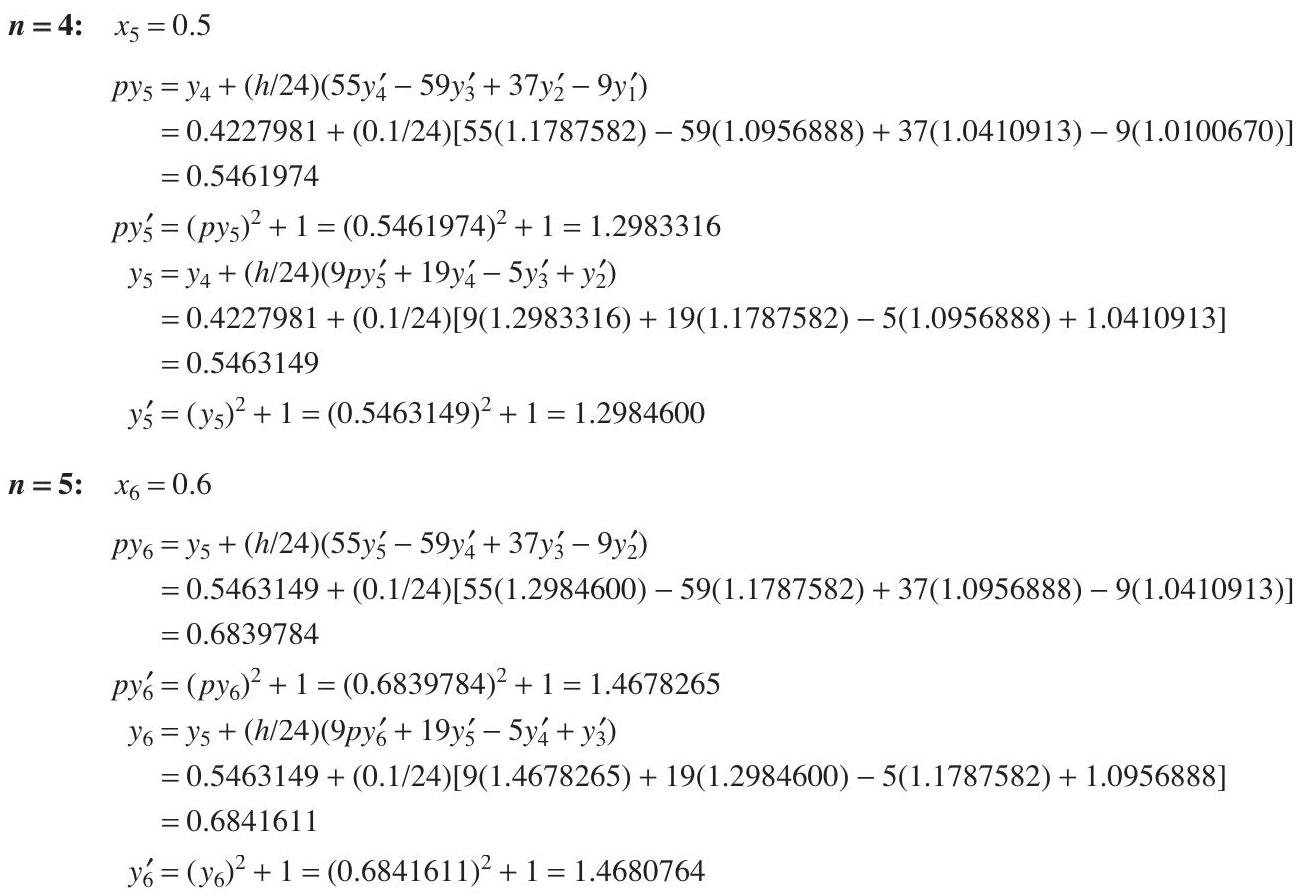
\includegraphics[max width=\textwidth]{2024_04_03_5bb5b4275a64cb9887d1g-205}
\end{center}

Continuing in this manner, we generate Table 19-7.

Table 19-7

\begin{center}
\begin{tabular}{|c|c|c|c|}
\hline
\multirow{2}{*}{}\begin{tabular}{l}
Method: \\
Problem: \\
\end{tabular} & \multicolumn{3}{|c|}{ADAMS-BASHFORTH-MOULTON METHOD} \\
\hline
 & \multicolumn{3}{|c|}{$y^{\prime}=y^{2}+1 ; y(0)=0$} \\
\hline
\multirow[t]{2}{*}{$x_{n}$} & \multicolumn{2}{|c|}{$h=0.1$} & \multirow{2}{*}{}\begin{tabular}{l}
True solution \\
$Y(x)=\tan x$ \\
\end{tabular} \\
\hline
 & $p y_{n}$ & $y_{n}$ &  \\
\hline
0.0 & - & 0.0000000 & 0.0000090 \\
\hline
0.1 & - & 0.1003346 & 0.1003347 \\
\hline
0.2 & - & 0.2027099 & 0.2027100 \\
\hline
0.3 & - & 0.3093360 & 0.3093363 \\
\hline
0.4 & 0.4227151 & 0.4227981 & 0.4227932 \\
\hline
0.5 & 0.5461974 & 0.5463149 & 0.5463025 \\
\hline
0.6 & 0.6839784 & 0.6841611 & 0.6841368 \\
\hline
0.7 & 0.8420274 & 0.8423319 & 0.8422884 \\
\hline
0.8 & 1.0291713 & 1.0297142 & 1.0296386 \\
\hline
0.9 & 1.2592473 & 1.2602880 & 1.2601582 \\
\hline
1.0 & 1.5554514 & 1.5576256 & 1.5574077 \\
\hline
\end{tabular}
\end{center}

19.9. Use the Adams-Bashforth-Moulton method to solve $y^{\prime}=2 x y /\left(x^{2}-y^{2}\right) ; y(1)=3$ on the interval $[1,2]$ with $h=0.2$.

Here $f(x, y)=2 x y /\left(x^{2}-y^{2}\right), x_{0}=1$ and $y_{0}=3$. With $h=0.2, x_{1}=x_{0}+h=1.2, x_{2}=x_{1}+h=1.4$, and $x_{3}=x_{2}+h=1.6$. Using the Runge-Kutta method to obtain the corresponding $y$-values needed to start the Adams-Bashforth-Moulton method, we find $y_{1}=2.8232844, y_{2}=2.5709342$, and $y_{3}=2.1321698$. It then follows from Eq. (19.3) that

$$
\begin{aligned}
& y_{0}^{\prime}=\frac{2 x_{0} y_{0}}{\left(x_{0}\right)^{2}-\left(y_{0}\right)^{2}}=\frac{2(1)(3)}{(1)^{2}-(3)^{2}}=-0.75 \\
& y_{1}^{\prime}=\frac{2 x_{1} y_{1}}{\left(x_{1}\right)^{2}-\left(y_{1}\right)^{2}}=\frac{2(1.2)(2.8232844)}{(1.2)^{2}-(2.8232844)^{2}}=-1.0375058 \\
& y_{2}^{\prime}=\frac{2 x_{2} y_{2}}{\left(x_{2}\right)^{2}-\left(y_{2}\right)^{2}}=\frac{2(1.4)(2.5709342)}{(1.4)^{2}-(2.5709342)^{2}}=-1.5481884 \\
& y_{3}^{\prime}=\frac{2 x_{3} y_{3}}{\left(x_{3}\right)^{2}-\left(y_{3}\right)^{2}}=\frac{2(1.6)(2.1321698)}{(1.6)^{2}-(2.1321698)^{2}}=-3.4352644
\end{aligned}
$$

Then, using Eqs. (19.6), beginning with $n=3$, and Eq. (19.3), we compute

$$
\begin{aligned}
n=3: \quad x_{4} & =1.8 \\
p y_{4} & =y_{3}+(h / 24)\left(55 y_{3}^{\prime}-59 y_{2}^{\prime}+37 y_{1}^{\prime}-9 y_{0}^{\prime}\right) \\
& =2.1321698+(0.1 / 24)[55(-3.4352644)-59(-1.5481884)+37(-1.0375058)-9(-0.75)] \\
& =1.0552186 \\
p y_{4}^{\prime} & =\frac{2 x_{4} p y_{4}}{\left(x_{4}\right)^{2}-\left(p y_{4}\right)^{2}}=\frac{2(1.8)(1.0552186)}{(1.8)^{2}-(1.0552186)^{2}}=1.7863919 \\
y_{4} & =y_{3}+(h / 24)\left(9 p y_{4}^{\prime}+19 y_{3}^{\prime}-5 y_{2}^{\prime}+y_{1}^{\prime}\right) \\
& =2.1321698+(0.1 / 24)[9(1.7863919)+19(-3.4352644)-5(-1.5481884)-(-1.0375058)] \\
& =1.7780943 \\
y_{4}^{\prime} & =\frac{2 x_{4} y_{4}}{\left(x_{4}\right)^{2}-\left(y_{4}\right)^{2}}=\frac{2(1.8)(1.7780943)}{(1.8)^{2}-(1.7780943)^{2}}=81.6671689 \\
x_{5}= & 2.0 \\
p y_{5} & =y_{4}+(h / 24)\left(55 y_{4}^{\prime}-59 y_{3}^{\prime}+37 y_{2}^{\prime}-9 y_{1}^{\prime}\right) \\
& =1.7780943+(0.1 / 24)[55(81.6671689)-59(-3.4352644)+37(-1.5481884)-9(-1.0375058)] \\
& =40.4983398 \\
p y_{5}^{\prime} & =\frac{2 x_{5} p y_{5}}{\left(x_{5}\right)^{2}-\left(p y_{5}\right)^{2}}=\frac{2(2.0)(40.4983398)}{(2.0)^{2}-(40.4983398)^{2}}=-0.0990110 \\
y_{5} & =y_{4}+(h / 24)\left(9 p y_{5}^{\prime}+19 y_{4}^{\prime}-5 y_{3}^{\prime}+y_{2}^{\prime}\right) \\
& =1.17780943+(0.1 / 24)[9(-0.0990110)+19(81.6671689)-5(-3.4352644)+(-1.5481884)] \\
& =14.8315380 \\
y_{5}^{\prime} & =\frac{2 x_{5} y_{5}}{\left(x_{5}\right)^{2}-\left(y_{5}\right)^{2}}=\frac{2(2.0)(14.8315380)}{(2.0)^{2}-(14.8315380)^{2}}=-0.2746905
\end{aligned}
$$

These results are troubling because the corrected values are not close to the predicted values as they should be. Note that $y_{5}$ is significantly different from $p y_{5}$ and $y_{4}^{\prime}$ is significantly different from $p y_{4}^{\prime}$. In any predictor-corrector method, the corrected values of $y$ and $y^{\prime}$ represent a fine-tuning of the predicted values, and not a major change. When significant changes occur, they are often the result of numerical instability, which can be remedied by a smaller step-size. Sometimes, however, significant differences arise because of a singularity in the solution.

In the computations above, note that the derivative at $x=1.8$, namely 81.667 , generates a nearly vertical slope and suggests a possible singularity near 1.8. Figure 19-1 is a direction field for this differential equation. On this

\begin{center}
\begin{tabular}{|c|c|c|c|c|c|c|c|c|c|c|c|c|c|c|c|c|c|c|c|c|c|c|c|c|}
\hline
1 & 1 & 1 & 1 & 1 & 1 & 1 & $\prime$ & $\prime$ & - & - & - & - & - & $\lambda$ & - & le &  &  &  &  & । & / & $/$ & / \\
\hline
1 & 1 & 1 & 1 & 1 & 1 & 1 & 1 & $\prime$ & - & - & - & $y-$ & - & - & - & 1 & 1 & 1 & $\backslash$ & 1 & 1 & / & , & , \\
\hline
$\backslash$ & $\backslash$ & $\backslash$ & 1 & 1 & 1 & 1 & $/$ & $/$ & $\prime$ & - & - & $\uparrow-$ & $\backslash$ & $\checkmark$ & 1 & 1 & 1 & 1 & 1 & 1 & , & $\prime$ & $\prime$ & $\prime$ \\
\hline
$\backslash$ & $\backslash$ & $\backslash$ & 1 & 1 & 1 & 1 & I & $/$ & $\prime$ & $\prime$ & - & - & $\backslash$ & $y$ & 1 & 1 & 1 & 1 & 1 & $/$ & 1 & $\prime$ & , & ' \\
\hline
$\backslash$ & $\backslash$ & $\backslash$ & $\backslash$ & 1 & 1 & 1 & 1 & / & $/$ & $\prime$ & $\prime$ & - & $\backslash$ & 1 & 1 & 1 & 1 & $i$ & I & 1 & $\prime$ & $\prime$ & $\prime$ & 1 \\
\hline
$\backslash$ & $\backslash$ & $\backslash$ & $\backslash$ & $\backslash$ & $\backslash$ & 1 & I & 1 & 1 & I & $\prime$ & - & $\backslash$ & 1 & 11 & 1 & $i$ & 1 & $/$ & 1 & $\prime$ & $\prime$ & $\prime$ & ' \\
\hline
$\backslash$ & $\backslash$ & $\backslash$ & $\backslash$ & $\backslash$ & $\backslash$ & 1 & 1 & $I$ & 1 & 1 & $\prime$ & - & $\backslash$ & 1 & 11 & 1 & 1 & 1 & $/$ & $\prime$ & $\prime$ & $\prime$ & ' & ' \\
\hline
$\backslash$ & $\backslash$ & $\backslash$ & $\backslash$ & $\backslash$ & $\backslash$ & 1 & 1 & 1 & 1 & 1 & 1 & - & $\backslash$ & 1 & $\sqrt{ }$ & 1 & $/$ & $\prime$ & $\prime$ & $\prime$ & $\prime$ & ' & - & - \\
\hline
- & - & $\checkmark$ & - & $\backslash$ & $\backslash$ & 1 & 1 & 1 & I & 1 & 1 & - & $\backslash$ & 1 & $1^{v}$ & 1 & $/$ & $\prime$ & $\prime$ & ' & - & - & - & - \\
\hline
- & - & - & - & $\backslash$ & $\backslash$ & $\backslash$ & 1 & 1 & 1 & 1 & 1 & - & 1 & 1 & 1 & 1 & 1 & $\prime$ & - & - & - & - & - & - \\
\hline
- & - & - & - & - & $\backslash$ & $\backslash$ & $\backslash$ & $\backslash$ & 1 & 1 & 1 & - & 1 & $i$ & 1 & 1 & $\prime$ & ' & - & - & - & - & - & - \\
\hline
- & - & - & - & - & - & $\backslash$ & $\backslash$ & $\backslash$ & $\backslash$ & 1 & 1 & - &  & 1 & 1 & 1 & ' & - & - & - & - & - & - & - \\
\hline
- & - & - & - & - & - & , & , & 1 & $/$ & 1 & 1 & - &  & 1 & 1 & 1 & $\backslash$ & $\backslash$ & - & - & - & - & - & - \\
\hline
- & - & - & - & - & - & ' & $\prime$ & 1 & / & 1 & 1 & - & $i$ & 1 & $\backslash$ & $\backslash$ & $\backslash$ & $\backslash$ & $\backslash$ & - & - & - & - & - \\
\hline
- & - & - & - & - & ' & $\prime$ & 1 & 1 & 1 & 1 & $i$ & - & 1 & $i$ & 1 & 1 & $\backslash$ & 1 & $\backslash$ & $\backslash$ & - & - & - & - \\
\hline
- & - & - & - & ' & $\prime$ & 1 & 1 & 1 & 1 & 1 & 1 & - & ' & 1 & 1 & 1 & $\backslash$ & 1 & $\backslash$ & $\backslash$ & - & - & - & - \\
\hline
- & - & - & ' & $\prime$ & $\prime$ & 1 & 1 & 1 & 1 & $\backslash$ & $\backslash$ & - & I & ' & ' &  & 1 & $\backslash$ & $\backslash$ & $\backslash$ & $\backslash$ & $\backslash$ & $\backslash$ & 〉 \\
\hline
' & ' & $\prime$ & $\prime$ & $\prime$ & 1 & 1 & 1 & 1 & $\backslash$ & $\backslash$ & 1 & - & 1 & 7 & 7 & 1 & 1 & 1 & $\backslash$ & $\backslash$ & $\backslash$ & $\backslash$ & $\backslash$ & $\backslash$ \\
\hline
$\prime$ & $\prime$ & $\prime$ & $\prime$ & 1 & 1 & 1 & 1 & 1 & 1 & 1 & $\backslash$ & - & $'$ & ' & ' & 1 & 1 & 1 & 1 & 1 & $\backslash$ & $\backslash$ & $\backslash$ & $\backslash$ \\
\hline
$\prime$ & $\prime$ & $\prime$ & 1 & 1 & 1 & 1 & 1 & 1 & $\backslash$ & $\backslash$ & $\backslash$ & - & ' & $\prime$ & 1 & 1 & 7 & 1 & $\backslash$ & 1 & $\backslash$ & $\backslash$ & $\backslash$ & $\backslash$ \\
\hline
$\prime$ & $\prime$ & $\prime$ & 1 & 1 & 1 & 1 & 1 & 1 & 1 & $\backslash$ & $\backslash$ & - & ' & $'$ & ' & 1 & 1 & 1 & 1 & $\backslash$ & 1 & $\backslash$ & $\backslash$ & $\backslash$ \\
\hline
$\prime$ & $\prime$ & $\prime$ & I & I & 1 & 1 & 1 & 1 & $\backslash$ & $\backslash$ & ' & - & - & ' & $\prime$ & 1 & I & $f$ & 1 & 1 & 1 & $\backslash$ & $\backslash$ & 1 \\
\hline
' & ' & 1 & 1 & 1 & 1 & 1 & 1 & $\backslash$ & $\backslash$ & 〉 & - & - & - & - & ' & $\prime$ & 1 & 1 & 1 & 1 & 1 & $\backslash$ & $\backslash$ & $\backslash$ \\
\hline
/ & I & 1 & 1 & 1 & $\backslash$ & 1 & 1 & $\backslash$ & $\backslash$ & - & - & - & - & - & - & $\prime$ & $\prime$ & 1 & 7 & 1 & 1 & $\backslash$ & 1 & 1 \\
\hline
\end{tabular}
\end{center}

Fig. 19.1

direction field we have plotted the points $\left(x_{0}, y_{0}\right)$ through $\left(x_{4}, y_{4}\right)$ as determined by the Adams-Bashforth-Moulton method and then sketched the solution curve through these points consistent with the direction field. The cusp between 1.6 and 1.8 is a clear indicator of a problem.

The analytic solution to the differential equation is given in Problem 4.14 as $x^{2}+y^{2}=k y$. Applying the initial condition, we find $k=10 / 3$, and then using the quadratic formula to solve explicitly for $y$, we obtain the solution

$$
y=\frac{5+\sqrt{25-9 x^{2}}}{3}
$$

This solution is only defined through $x=5 / 3$ and is undefined after that.

19.10. Redo Problem 19.7 using Milne's method.

The values of $y_{0}, y_{1}, y_{2}, y_{3}$, and their derivatives are exactly as given in Problem 19.7. Using Eqs. (19.7) and (19.3), we compute

$$
\begin{aligned}
n=3: \quad p y_{4} & =y_{0}+\frac{4 h}{3}\left(2 y_{3}^{\prime}-y_{2}^{\prime}+2 y_{1}^{\prime}\right) \\
& =2+\frac{4(0.1)}{3}[2(2.3498585)-2.2214026+2(2.1051708)] \\
& =2.8918208 \\
p y_{4}^{\prime} & =p y_{4}-x_{4}=2.4918208 \\
y_{4} & =y_{2}+\frac{h}{3}\left(p y_{4}^{\prime}+4 y_{3}^{\prime}+y_{2}^{\prime}\right) \\
& =2.4214026+\frac{0.1}{3}[2.4918208+4(2.3498585)+2.2214026] \\
& =2.8918245
\end{aligned}
$$

$$
\begin{aligned}
n=4: x_{4} & =0.4, \quad y_{4}^{\prime}=y_{4}-x_{4}=2.4918245 \\
p y_{5} & =y_{1}+\frac{4 h}{3}\left(2 y_{4}^{\prime}-y_{3}^{\prime}+2 y_{2}^{\prime}\right) \\
& =2.2051708+\frac{4(0.1)}{3}[2(2.4918245)-2.3498585+2(2.2214026)] \\
& =3.1487169 \\
p y_{5}^{\prime} & =p y_{5}-x_{5}=2.6487169 \\
y_{5} & =y_{3}+\frac{h}{3}\left(p y_{5}^{\prime}+4 y_{4}^{\prime}+y_{3}^{\prime}\right) \\
& =2.6498585+\frac{0.1}{3}[2.6487169+4(2.4918245)+2.3498585] \\
& =3.1487209 \\
x_{5} & =0.5, \quad y_{5}^{\prime}=y_{5}-x_{5}=2.6487209 \\
p y_{6} & =y_{2}+\frac{4 h}{3}\left(2 y_{5}^{\prime}-y_{4}^{\prime}+2 y_{3}^{\prime}\right) \\
& =2.4214026+\frac{4(0.1)}{3}[2(2.6487209)-2.4918245+2(2.3498585)] \\
& =3.4221138 \\
p y_{6}^{\prime} & =p y_{6}-x_{6}=2.8221138 \\
y_{6}= & y_{4}+\frac{h}{3}\left(p y_{6}^{\prime}+4 y_{5}^{\prime}+y_{4}^{\prime}\right) \\
= & 2.8918245+\frac{0.1}{3}[2.8221138+4(2.6487209)+2.4918245] \\
= & 3.4221186
\end{aligned}
$$

Continuing in this manner, we generate Table 19-8.

19.11. Redo Problem 19.8 using Milne's method.

The values of $y_{0}, y_{1}, y_{2}, y_{3}$, and their derivatives are exactly as given in Problem 19.8. Using Eqs. (19.7) and (19.3), we compute

$$
\begin{array}{rl}
n=3: \quad p y_{4} & =y_{0}+\frac{4 h}{3}\left(2 y_{3}^{\prime}-y_{2}^{\prime}+2 y_{1}^{\prime}\right) \\
& =0+\frac{4(0.1)}{3}[2(1.0956888)-1.0410913+2(1.0100670)] \\
& =0.4227227 \\
p y_{4}^{\prime} & =\left(p y_{4}\right)^{2}+1=(0.4227227)^{2}+1=1.1786945 \\
y_{4} & =y_{2}+\frac{h}{3}\left(p y_{4}^{\prime}+4 y_{3}^{\prime}+y_{2}^{\prime}\right) \\
& =0.2027099+\frac{0.1}{3}[1.1786945+4(1.0956888)+1.0410913] \\
& =0.4227946 \\
\mathbf{n = 4 :} \quad x_{4} & 0.4, \quad y_{4}^{\prime}=\left(y_{4}\right)^{2}+1=(0.4227946)^{2}+1=1.1787553 \\
p y_{5} & =y_{1}+\frac{4 h}{3}\left(2 y_{4}^{\prime}-y_{3}^{\prime}+2 y_{2}^{\prime}\right) \\
& =0.1003346+\frac{4(0.1)}{3}[2(1.1787553)-1.0956888+2(1.0410913)] \\
& =0.5462019
\end{array}
$$

Table 19-8

\begin{center}
\begin{tabular}{|c|c|c|c|}
\hline
\multicolumn{3}{|c|}{Method: MILNE'S METHOD} &  \\
\hline
\multicolumn{3}{|c|}{Problem: $y^{\prime}=y-x ; y(0)=2$} & \multirow{2}{c|}{True solution} \\
\cline { 1 - 3 }
$x_{n}$ & \multicolumn{2}{|c|}{$h=0.1$} &  \\
\cline { 2 - 4 }
 & $p y_{n}$ & $y_{n}$ & 2.0000000 \\
\hline
0.0 & - & 2.0000000 & 2.2051709 \\
\hline
0.1 & - & 2.2051708 & 2.4214028 \\
\hline
0.2 & - & 2.4214026 & 2.6498588 \\
\hline
0.3 & - & 2.6498585 & 2.8918247 \\
\hline
0.4 & 2.8918208 & 2.8918245 & 3.1487213 \\
\hline
0.5 & 3.1487169 & 3.1487209 & 3.4221188 \\
\hline
0.6 & 3.4221138 & 3.4221186 & 3.7137527 \\
\hline
0.7 & 3.7137472 & 3.7137524 & 4.0255409 \\
\hline
0.8 & 4.0255349 & 4.0255407 & 4.3596031 \\
\hline
0.9 & 4.3595964 & 4.3596027 & 4.7182818 \\
\hline
1.0 & 4.7182745 & 4.7182815 &  \\
\hline
 &  &  &  \\
\hline
\end{tabular}
\end{center}

$$
\begin{aligned}
p y_{5}^{\prime} & =\left(p y_{5}\right)+1=(0.5462019)^{2}+1=1.2983365 \\
y_{5} & =y_{3}+\frac{h}{3}\left(p y_{5}^{\prime}+4 y_{4}^{\prime}+y_{3}^{\prime}\right) \\
& =0.3093360+\frac{0.1}{3}[1.2983365+4(1.1787553)+1.0956888] \\
& =0.5463042
\end{aligned}
$$

$$
\begin{aligned}
\mathbf{n = 5 :} x_{5}= & 0.5, \quad y_{5}^{\prime}=\left(y_{5}\right)^{2}+1=(0.5463042)^{2}+1=1.2984483 \\
p y_{6} & =y_{2}+\frac{4 h}{3}\left(2 y_{5}^{\prime}-y_{4}^{\prime}+2 y_{3}^{\prime}\right) \\
& =0.2027099+\frac{4(0.1)}{3}[2(1.2984483)-1.1787553+2(1.0956888)] \\
& =0.6839791 \\
p y_{6}^{\prime} & =\left(p y_{6}\right)^{2}+1=(0.6839791)^{2}+1=1.4678274 \\
y_{6} & =y_{4}+\frac{h}{3}\left(p y_{6}^{\prime}+4 y_{5}^{\prime}+y_{4}^{\prime}\right) \\
& =0.4227946+\frac{0.1}{3}[1.4678274+4(1.2984483)+1.1787553] \\
& =0.6841405
\end{aligned}
$$

Continuing in this manner, we generate Table 19-9.

Table 19-9

\begin{center}
\begin{tabular}{|c|c|c|c|}
\hline
 & Method & \multicolumn{2}{|c|}{MILNE'S METHOD} \\
\hline
\multicolumn{4}{|c|}{Problem:} \\
\hline
\multirow[t]{2}{*}{$x_{n}$} & \multicolumn{2}{|c|}{$h=0.1$} & \multirow{2}{*}{}\begin{tabular}{l}
True solution \\
$Y(x)=\tan x$ \\
\end{tabular} \\
\hline
 & $p y_{n}$ & $y_{n}$ &  \\
\hline
0.0 & - & 0.0000000 & 0.0000000 \\
\hline
0.1 & - & 0.1003346 & 0.1003347 \\
\hline
0.2 & - & 0.2027099 & 0.2027100 \\
\hline
0.3 & - & 0.3093360 & 0.3093363 \\
\hline
0.4 & 0.4227227 & 0.4227946 & 0.4227932 \\
\hline
0.5 & 0.5462019 & 0.5463042 & 0.5463025 \\
\hline
0.6 & 0.6839791 & 0.6841405 & 0.6841368 \\
\hline
0.7 & 0.8420238 & 0.8422924 & 0.8422884 \\
\hline
0.8 & 1.0291628 & 1.0296421 & 1.0296386 \\
\hline
0.9 & 1.2592330 & 1.2601516 & 1.2601582 \\
\hline
1.0 & 1.5554357 & 1.5573578 & 1.5574077 \\
\hline
\end{tabular}
\end{center}

19.12. Use Milne's method to solve $y^{\prime}=y ; y(0)=1$ on the interval $[0,1]$ with $h=0.1$.

Here $f(x, y)=y, x_{0}=0$, and $y_{0}=1$. From Table 19-4, we find as the three additional starting values $y_{1}=1.1051708, y_{2}=1.2214026$, and $y_{3}=1.3498585$. Note that $y_{1}^{\prime}=y_{1}, y_{2}^{\prime}=y_{2}$, and $y_{3}^{\prime}=y_{3}$. Then, using Eqs. (19.7) and (19.3) and we compute

$$
\begin{aligned}
n=3: \quad p y_{4} & =y_{0}+\frac{4 h}{3}\left(2 y_{3}^{\prime}-y_{2}^{\prime}+2 y_{1}^{\prime}\right) \\
& =1+\frac{4(0.1)}{3}[2(1.3498585)-1.2214026+2(1.1051708)] \\
& =1.4918208 \\
p y_{4}^{\prime} & =p y_{4}=1.4918208 \\
y_{4} & =y_{2}+\frac{h}{3}\left(p y_{4}^{\prime}+4 y_{3}^{\prime}+y_{2}^{\prime}\right) \\
& =1.2214026+\frac{0.1}{3}[1.4918208+4(1.3498585)+1.2214026] \\
& =1.4918245 \\
x_{4} & =0.4, \quad y_{4}^{\prime}=y_{4}=1.4918245 \\
p y_{5} & =y_{1}+\frac{4 h}{3}\left(2 y_{4}^{\prime}-y_{3}^{\prime}+2 y_{2}^{\prime}\right) \\
& =1.1051708+\frac{4(0.1)}{3}[2(1.4918245)-1.3498585+2(1.2214026)] \\
& =1.6487169
\end{aligned}
$$

$$
\begin{aligned}
p y_{5}^{\prime} & =p y_{5}=1.6487169 \\
y_{5} & =y_{3}+\frac{h}{3}\left(p y_{5}^{\prime}+4 y_{4}^{\prime}+y_{3}^{\prime}\right) \\
& =1.3498585+\frac{0.1}{3}[1.6487169+4(1.4918245)+1.3498585] \\
& =1.6487209 \\
\boldsymbol{n}=\mathbf{5}: \quad x_{5} & =0.5, \quad y_{5}^{\prime}=y_{5}=1.6487209 \\
p y_{6} & =y_{2}+\frac{4 h}{3}\left(2 y_{5}^{\prime}-y_{4}^{\prime}+2 y_{3}^{\prime}\right) \\
& =1.2214026+\frac{4(0.1)}{3}[2(1.6487209)-1.4918245+2(1.3498585)] \\
& =1.8221138 \\
p y_{6}^{\prime} & =p y_{6}=1.8221138 \\
y_{6} & =y_{4}+\frac{h}{3}\left(p y_{6}^{\prime}+4 y_{5}^{\prime}+y_{4}^{\prime}\right) \\
& =1.4918245+\frac{0.1}{3}[1.8221138+4(1.6487209)+1.4918245] \\
& =1.8221186
\end{aligned}
$$

\begin{center}
\begin{tabular}{|c|c|c|c|}
\hline
 & Method & \multicolumn{2}{|c|}{MILNE'S METHOD} \\
\hline
\multicolumn{4}{|c|}{Problem:} \\
\hline
\multirow[t]{2}{*}{$x_{n}$} & \multicolumn{2}{|c|}{$h=0.1$} & \multirow{2}{*}{}\begin{tabular}{l}
True solution \\
$\qquad Y(x)=e^{x}$ \\
\end{tabular} \\
\hline
 & $p y_{n}$ & $y_{n}$ &  \\
\hline
0.0 & - & 1.0000000 & 1.0000000 \\
\hline
0.1 & - & 1.1051708 & 1.1051709 \\
\hline
0.2 & - & 1.2214026 & 1.2214028 \\
\hline
0.3 & - & 1.3498585 & 1.3498588 \\
\hline
0.4 & 1.4918208 & 1.4918245 & 1.4918247 \\
\hline
0.5 & 1.6487169 & 1.6487209 & 1.6487213 \\
\hline
0.6 & 1.8221138 & 1.8221186 & 1.8221188 \\
\hline
0.7 & 2.0137472 & 2.0137524 & 2.0137527 \\
\hline
0.8 & 2.2255349 & 2.2255407 & 2.2255409 \\
\hline
0.9 & 2.4595964 & 2.4596027 & 2.4596031 \\
\hline
1.0 & 2.7182745 & 2.7182815 & 2.7182818 \\
\hline
\end{tabular}
\end{center}

Continuing in this manner, we generate Table 19-10.

Table 19-10

\section*{Supplementary Problems}
Carry all computations to three decimal places.

19.13. Use the modified Euler's method to solve $y^{\prime}=-y+x+2 ; y(0)=2$ on the interval $[0,1]$ with $h=0.1$.

19.14. Use the modified Euler's method to solve $y^{\prime}=-y ; y(0)=1$ on the interval $[0,1]$ with $h=0.1$.

19.15. Use the modified Euler's method to solve $y^{\prime}=\frac{x^{2}+y^{2}}{x y} ; y(1)=3$ on the interval $[1,2]$ with $h=0.2$.

19.16. Use the modified Euler's method to solve $y^{\prime}=x ; y(2)=1$ on the interval $[2,3]$ with $h=0.25$.

19.17. Use the modified Euler's method to solve $y^{\prime}=4 x^{3} ; y(2)=6$ on the interval $[2,3]$ with $h=0.2$.

19.18. Redo Problem 19.13 using the Runge-Kutta method.

19.19. Redo Problem 19.14 using the Runge-Kutta method.

19.20. Redo Problem 19.15 using the Runge-Kutta method.

19.21. Redo Problem 19.17 using the Runge-Kutta method.

19.22. Use the Runge-Kutta method to solve $y^{\prime}=5 x^{4} ; y(0)=0$ on the interval $[0,1]$ with $h=0.1$.

19.23. Use the Adams-Bashforth-Moulton method to solve $y^{\prime}=y ; y(0)=1$ on the interval $[0,1]$ with $h=0.1$.

19.24. Redo Problem 19.13 using the Adams-Bashforth-Moulton method.

19.25. Redo Problem 19.14 using the Adams-Bashforth-Moulton method.

19.26. Redo Problem 19.15 using the Adams-Bashforth-Moulton method.

19.27. Redo Problem 19.13 using Milne's method.

19.28. Redo Problem 19.14 using Milne's method.

\section*{$\rightarrow$ Numerical Methods for Solving Second-Order Differential Equations Via Systems}
\section*{SECOND-ORDER DIFFERENTIAL EQUATIONS}
In Chapter 17, we showed how a second (or higher)-order differential equation could be expressed as a system of first-order differential equations.

In this chapter we investigate several numerical techniques dealing with such systems.

In the following system of initial-value problems, $y$ and $z$ are functions of $x$ :


\begin{align*}
& y^{\prime}=f(x, y, z) \\
& z^{\prime}=g(x, y, z)  \tag{20.1}\\
& y\left(x_{0}\right)=y_{0}, z\left(x_{0}\right)=z_{0}
\end{align*}


We note that, with $y^{\prime}=f(x, y, z) \equiv z$, System (20.1) represents the second-order initial-value problem

$$
y^{\prime \prime}=g\left(x, y, y^{\prime}\right) ; \quad y\left(x_{0}\right)=y_{0}, \quad y^{\prime}\left(x_{0}\right)=z_{0}
$$

Standard form for a system of three equations is


\begin{align*}
& y^{\prime}=f(x, y, z, w) \\
& z^{\prime}=g(x, y, z, w)  \tag{20.2}\\
& w^{\prime}=r(x, y, z, w) \\
& y\left(x_{0}\right)=y_{0}, z\left(x_{0}\right)=z_{0}, w\left(x_{0}\right)=w_{0}
\end{align*}


If, in such a system, $f(x, y, z, w)=z$, and $g(x, y, z, w)=w$, then system (20.2) represents the third-order initialvalue problem

$$
y^{\prime \prime \prime}=r(x, y, z, w) ; \quad y\left(x_{0}\right)=y_{0}, \quad y^{\prime}\left(x_{0}\right)=z_{0}, \quad y^{\prime \prime}\left(x_{0}\right)=w_{0}
$$

The formulas that follow are for systems of two equations in standard form (20.1) Generalizations to systems of three equations in standard form (20.2) or systems with four or more equations are straightforward.

\section*{EULER'S METHOD}

\begin{align*}
& y_{n+1}=y_{n}+h y_{n}^{\prime}  \tag{20.3}\\
& z_{n+1}=z_{n}+h z_{n}^{\prime}
\end{align*}


\section*{RUNGE-KUTTA METHOD}

\begin{align*}
& y_{n+1}=y_{n}+\frac{1}{6}\left(k_{1}+2 k_{2}+2 k_{3}+k_{4}\right)  \tag{20.4}\\
& z_{n+1}=z_{n}+\frac{1}{6}\left(l_{1}+2 l_{2}+2 l_{3}+l_{4}\right)
\end{align*}


where $k_{1}=h f\left(x_{n}, y_{n}, z_{n}\right)$

$l_{1}=h g\left(x_{n}, y_{n}, z_{n}\right)$

$k_{2}=h f\left(x_{n}+\frac{1}{2} h, y_{n}+\frac{1}{2} k_{1}, z_{n}+\frac{1}{2} l_{1}\right)$

$l_{2}=h g\left(x_{n}+\frac{1}{2} h, y_{n}+\frac{1}{2} k_{1}, z_{n}+\frac{1}{2} l_{1}\right)$

$k_{3}=h f\left(x_{n}+\frac{1}{2} h, y_{n}+\frac{1}{2} k_{2}, z_{n}+\frac{1}{2} l_{2}\right)$

$l_{3}=h g\left(x_{n}+\frac{1}{2} h, y_{n}+\frac{1}{2} k_{2}, z_{n}+\frac{1}{2} l_{2}\right)$

$k_{4}=h f\left(x_{n}+h, y_{n}+k_{3}, z_{n}+l_{3}\right)$

$l_{4}=h g\left(x_{n}+h, y_{n}+k_{3}, z_{n}+l_{3}\right)$

\section*{ADAMS-BASHFORTH-MOULTON METHOD}
$$
\begin{aligned}
& \text { predictors: } \quad p y_{n+1}=y_{n}+\frac{h}{24}\left(55 y_{n}^{\prime}-59 y_{n-1}^{\prime}+37 y_{n-2}^{\prime}-9 y_{n-3}^{\prime}\right) \\
& p z_{n+1}=z_{n}+\frac{h}{24}\left(55 z_{n}^{\prime}-59 z_{n-1}^{\prime}+37 z_{n-2}^{\prime}-9 z_{n-3}^{\prime}\right) \\
& \text { correctors : } \quad y_{n+1}=y_{n}+\frac{h}{24}\left(9 p y_{n+1}^{\prime}+19 y_{n}^{\prime}-5 y_{n-1}^{\prime}+y_{n-2}^{\prime}\right) \\
& z_{n+1}=z_{n}+\frac{h}{24}\left(9 p z_{n+1}^{\prime}+19 z_{n}^{\prime}-5 z_{n-1}^{\prime}+z_{n-2}^{\prime}\right)
\end{aligned}
$$

Corresponding derivatives are calculated from System (20.1). In particular,


\begin{align*}
& y_{n+1}^{\prime}=f\left(x_{n+1}, y_{n+1}, z_{n+1}\right)  \tag{20.6}\\
& z_{n+1}^{\prime}=g\left(x_{n+1}, y_{n+1}, z_{n+1}\right)
\end{align*}


The derivatives associated with the predicted values are obtained similarly, by replacing $y$ and $z$ in Eq. (20.6) with $p y$ and $p z$, respectively. As in Chapter 19, four sets of starting values are required for the Adams-Bashforth-Moulton method. The first set comes directly from the initial conditions; the other three sets are obtained from the Runge-Kutta method.

\section*{Solved Problems}
20.1. Reduce the initial-value problem $y^{\prime \prime}-y=x ; y(0)=0, y^{\prime}(0)=1$ to System (20.1).

Defining $z=y^{\prime}$, we have $z(0)=y^{\prime}(0)=1$ and $z^{\prime}=y^{\prime \prime}$. The given differential equation can be rewritten as $y^{\prime \prime}=y+x$, or $z^{\prime}=y+x$. We thus obtain the first-order system

$$
\begin{aligned}
& y^{\prime}=z \\
& z^{\prime}=y+x \\
& y(0)=0, z(0)=1
\end{aligned}
$$

20.2. Reduce the initial-value problem $y^{\prime \prime}-3 y^{\prime}+2 y=0 ; y(0)=-1, y^{\prime}(0)=0$ to System (20.1).

Defining $z=y^{\prime}$, we have $z(0)=y^{\prime}(0)=0$ and $z^{\prime}=y^{\prime \prime}$. The given differential equation can be rewritten as $y^{\prime \prime}=3 y^{\prime}-2 y$, or $z^{\prime}=3 z-2 y$. We thus obtain the first-order system

$$
\begin{aligned}
& y^{\prime}=z \\
& z^{\prime}=3 z-2 y \\
& y(0)=-1, z(0)=0
\end{aligned}
$$

20.3. Reduce the initial-value problem $3 x^{2} y^{\prime \prime}-x y^{\prime}+y=0 ; y(1)=4, y^{\prime}(1)=2$ to $\operatorname{System}(20.1)$.

Defining $z=y^{\prime}$, we have $z(1)=y^{\prime}(1)=2$, and $z^{\prime}=y^{\prime \prime}$. The given differential equation can be rewritten as

$$
\begin{aligned}
& y^{\prime \prime}=\frac{x y^{\prime}-y}{3 x^{2}} \\
& z^{\prime}=\frac{x z-y}{3 x^{2}}
\end{aligned}
$$

We thus obtain the first-order system

$$
\begin{aligned}
& y^{\prime}=z \\
& z^{\prime}=\frac{x z-y}{3 x^{2}} \\
& y(1)=4, z(1)=2
\end{aligned}
$$

20.4. Reduce the initial-value problem $y^{\prime \prime \prime}-2 x y^{\prime \prime}+4 y^{\prime}-x^{2} y=1 ; y(0)=1, y^{\prime}(0)=2, y^{\prime \prime}(0)=3$ to System (20.2).

Following Steps 1 through 3 of Chapter 17, we obtain the system

$$
\begin{aligned}
& y_{1}^{\prime}=y_{2} \\
& y_{2}^{\prime}=y_{3} \\
& y_{3}^{\prime}=x^{2} y_{1}-4 y_{2}+2 x y_{3}+1 ; \\
& y_{1}(0)=1, y_{2}(0)=2, y_{3}(0)=3
\end{aligned}
$$

To eliminate subscripting, we define $y=y_{1}, z=y_{2}$, and $w=y_{3}$. The system then becomes

$$
\begin{aligned}
& y^{\prime}=z \\
& z^{\prime}=w \\
& w^{\prime}=x^{2} y-4 z+2 x w+1 ; \\
& y(0)=1, z(0)=2, w(0)=3
\end{aligned}
$$

20.5. Use Euler's method to solve $y^{\prime \prime}-y=x ; y(0)=0, y^{\prime}(0)=1$ on the interval $[0,1]$ with $h=0.1$.

Using the results of Problem 20.1, we have $f(x, y, z)=z, g(x, y, z)=y+x, x_{0}=0, y_{0}=0$, and $z_{0}=1$. Then, using (20.3), we compute

$$
\begin{array}{ll}
\mathbf{n = 0}: & y_{0}^{\prime}=f\left(x_{0}, y_{0}, z_{0}\right)=z_{0}=1 \\
& z_{0}^{\prime}=g\left(x_{0}, y_{0}, z_{0}\right)=y_{0}+x_{0}=0+0=0 \\
& y_{1}=y_{0}+h y_{0}^{\prime}=0+(0.1)(1)=0.1 \\
& z_{1}=z_{0}+h z_{0}^{\prime}=1+(0.1)(0)=1 \\
\boldsymbol{n}^{\prime}=\mathbf{1}: & y_{1}^{\prime}=f\left(x_{1}, y_{1}, z_{1}\right)=z_{1}=1 \\
z_{1}^{\prime} & =g\left(x_{1}, y_{1}, z_{1},\right)=y_{1}+x_{1}=0.1+0.1=0.2 \\
& y_{2}=y_{1}+h y_{1}^{\prime}=0.1+(0.1)(1)=0.2 \\
& z_{2}=z_{1}+h z_{1}^{\prime}=1+(0.1)(0.2)=1.02 \\
\mathbf{n = 2}: & y_{2}^{\prime}=f\left(x_{2}, y_{2}, z_{2}\right)=z_{2}=1.02 \\
& z_{2}^{\prime}=g\left(x_{2}, y_{2}, z_{2},\right)=y_{2}+x_{2}=0.2+0.2=0.4 \\
& y_{3}=y_{2}+h y_{2}^{\prime}=0.2+(0.1)(1.02)=0.302 \\
& z_{3}=z_{2}+h z_{2}^{\prime}=1.02+(0.1)(0.4)=1.06
\end{array}
$$

Continuing in this manner, we generate Table 20-1.

Table 20-1

\begin{center}
\begin{tabular}{|c|c|c|c|}
\hline
\multicolumn{3}{|c|}{Method: EULER'S METHOD} &  \\
\hline
\multicolumn{3}{|c|}{Problem: $y^{\prime \prime}-y=x ; y(0)=0, y^{\prime}(0)=1$} &  \\
\hline
$x_{n}$ & \multicolumn{2}{|c|}{$h=0.1$} & \multicolumn{1}{c|}{True solution} \\
\cline { 2 - 4 }
 & $y_{n}$ & $z_{n}$ & $Y(x)=e^{x}-e^{-x}-x$ \\
\hline
0.0 & 0.0000 & 1.0000 & 0.0000 \\
\hline
0.1 & 0.1000 & 1.0000 & 0.1003 \\
\hline
0.2 & 0.2000 & 1.0200 & 0.2027 \\
\hline
0.3 & 0.3020 & 1.0600 & 0.3090 \\
\hline
0.4 & 0.4080 & 1.1202 & 0.4215 \\
\hline
0.5 & 0.5200 & 1.2010 & 0.5422 \\
\hline
0.6 & 0.6401 & 1.3030 & 0.6733 \\
\hline
0.7 & 0.7704 & 1.4270 & 0.8172 \\
\hline
0.8 & 0.9131 & 1.5741 & 0.9762 \\
\hline
0.9 & 1.0705 & 1.7454 & 1.1530 \\
\hline
1.0 & 1.2451 & 1.9424 & 1.3504 \\
\hline
 &  &  &  \\
\hline
\end{tabular}
\end{center}

20.6. Use Euler's method to solve $y^{\prime \prime}-3 y^{\prime}+2 y=0 ; y(0)=-1, y^{\prime}(0)=0$ on the interval [0,1] with $h=0.1$.

Using the results of Problem 20.2, we have $f(x, y, z)=z, g(x, y, z)=3 z-2 y, x_{0}=0, y_{0}=-1$, and

$$
\begin{aligned}
z_{0}=0 . & \text { Then, using }(20.3), \text { we compute } \\
\boldsymbol{n}=\mathbf{0}: & y_{0}^{\prime}=f\left(x_{0}, y_{0}, z_{0}\right)=z_{0}=0 \\
& z_{0}^{\prime}=g\left(x_{0}, y_{0}, z_{0}\right)=3 z_{0}-2 y_{0}=3(0)-2(-1)=2 \\
y_{1} & =y_{0}+h y_{0}^{\prime}=-1+(0.1)(0)=-1 \\
z_{1} & =z_{0}+h z_{0}^{\prime}=0+(0.1)(2)=0.2 \\
\boldsymbol{n}=\mathbf{1}: & y_{1}^{\prime}=f\left(x_{1}, y_{1}, z_{1}\right)=z_{1}=0.2 \\
z_{1}^{\prime} & =g\left(x_{1}, y_{1}, z_{1}\right)=3 z_{1}-2 y_{1}=3(0.2)-2(-1)=2.6 \\
y_{2} & =y_{1}+h y_{1}^{\prime}=-1+(0.1)(0.2)=-0.98 \\
z_{2} & =z_{1}+h z_{1}^{\prime}=0.2+(0.1)(2.6)=0.46
\end{aligned}
$$

\begin{center}
\begin{tabular}{|c|c|c|c|}
\hline
\multicolumn{4}{|c|}{EULER'S METHOD} \\
\hline
 & Problem: & \multicolumn{2}{|c|}{$y^{\prime \prime}-3 y^{\prime}+2 y=0 ; y(0)=-1, y^{\prime}(0)=0$} \\
\hline
\multirow[t]{2}{*}{$x_{n}$} & \multicolumn{2}{|c|}{$h=0.1$} & \multirow{2}{*}{}\begin{tabular}{l}
True solution \\
$Y(x)=e^{2 x}-2 e^{x}$ \\
\end{tabular} \\
\hline
 & $y_{n}$ & $z_{n}$ &  \\
\hline
0.0 & -1.0000 & 0.0000 & -1.0000 \\
\hline
0.1 & -1.0000 & 0.2000 & -0.9889 \\
\hline
0.2 & -0.9800 & 0.4600 & -0.9510 \\
\hline
0.3 & -0.9340 & 0.7940 & -0.8776 \\
\hline
0.4 & -0.8546 & 1.2190 & -0.7581 \\
\hline
0.5 & -0.7327 & 1.7556 & -0.5792 \\
\hline
0.6 & -0.5571 & 2.4288 & -0.3241 \\
\hline
0.7 & -0.3143 & 3.2689 & 0.0277 \\
\hline
0.8 & 0.0126 & 4.3125 & 0.5020 \\
\hline
0.9 & 0.4439 & 5.6037 & 1.1304 \\
\hline
1.0 & 1.0043 & 7.1960 & 1.9525 \\
\hline
\end{tabular}
\end{center}

Continuing in this manner, we generate Table 20-2.

Table 20-2

20.7. Use the Runge-Kutta method to solve $y^{\prime \prime}-y=x ; y(0)=0, y^{\prime}(0)=1$ on the interval $[0,1]$ with $h=0.1$.

Using the results of Problem 20.1, we have $f(x, y, z)=z, g(x, y, z)=y+x, x_{0}=0, y_{0}=0$, and $z_{0}=1$. Then, using (20.4) and rounding all calculations to three decimal places, we compute:

$$
\mathbf{n = 0 :} \quad \begin{aligned}
k_{1} & =h f\left(x_{0}, y_{0}, z_{0}\right)=h f(0,0,1)=(0.1)(1)=0.1 \\
l_{1} & =h g\left(x_{0}, y_{0}, z_{0}\right)=h g(0,0,1)=(0.1)(0+0)=0 \\
k_{2} & =h f\left(x_{0}+\frac{1}{2} h, y_{0}+\frac{1}{2} k_{1}, z_{0}+\frac{1}{2} l_{1}\right) \\
& =h f\left[0+\frac{1}{2}(0.1), 0+\frac{1}{2}(0.1), 1+\frac{1}{2}(0)\right] \\
& =h f(0.05,0.05,1)=(0.1)(1)=0.1
\end{aligned}
$$

$$
\begin{aligned}
& l_{2}=h g\left(x_{0}+\frac{1}{2} h, y_{0}+\frac{1}{2} k_{1}, z_{0}+\frac{1}{2} l_{1}\right) \\
& =h g(0.05,0.05,1)=(0.1)(0.05+0.05)=0.01 \\
& k_{3}=h f\left(x_{0}+\frac{1}{2} h, y_{0}+\frac{1}{2} k_{2}, z_{0}+\frac{1}{2} l_{2}\right) \\
& =h f\left[0+\frac{1}{2}(0.1), 0+\frac{1}{2}(0.1), 1+\frac{1}{2}(0.01)\right] \\
& =h f(0.05,0.05,1.005)=(0.1)(1.005)=0.101 \\
& l_{3}=h g\left(x_{0}+\frac{1}{2} h, y_{0}+\frac{1}{2} k_{2}, z_{0}+\frac{1}{2} l_{2}\right) \\
& =h g(0.05,0.05,1.005)=(0.1)(0.05+0.05)=0.01 \\
& k_{4}=h f\left(x_{0}+h, y_{0}+k_{3}, z_{0}+l_{3}\right) \\
& =h f(0+0.1,0+0.101,1+0.01) \\
& =h f(0.1,0.101,1.01)=(0.1)(1.01)=0.101 \\
& l_{4}=h g\left(x_{0}+h, y_{0}+k_{3}, z_{0}+l_{3}\right) \\
& =h g(0.1,0.101,1.01)=(0.1)(0.101+0.1)=0.02 \\
& y_{1}=y_{0}+\frac{1}{6}\left(k_{1}+2 k_{2}+2 k_{3}+k_{4}\right) \\
& =0+\frac{1}{6}[0.1+2(0.1)+2(0.101)+(0.101)]=0.101 \\
& z_{1}=z_{0}+\frac{1}{6}\left(l_{1}+2 l_{2}+2 l_{3}+l_{4}\right) \\
& =1+\frac{1}{6}[0+2(0.01)+2(0.01)+(0.02)]=1.01 \\
& \boldsymbol{n}=\mathbf{1}: \quad k_{1}=h f\left(x_{1}, y_{1}, z_{1}\right)=h f(0.1,0.101,1.01) \\
& =(0.1)(1.01)=0.101 \\
& l_{1}=h g\left(x_{1}, y_{1}, z_{1}\right)=h g(0.1,0.101,1.01) \\
& =(0.1)(0.101+0.1)=0.02 \\
& k_{2}=h f\left(x_{1}+\frac{1}{2} h, y_{1}+\frac{1}{2} k_{1}, z_{1}+\frac{1}{2} l_{1}\right) \\
& =h f\left[0.1+\frac{1}{2}(0.1), 0.101+\frac{1}{2}(0.101), 1.01+\frac{1}{2}(0.02)\right] \\
& =h f(0.15,0.152,1.02)=(0.1)(1.02)=0.102 \\
& l_{2}=h g\left(x_{1}+\frac{1}{2} h, y_{1}+\frac{1}{2} k_{1}, z_{1}+\frac{1}{2} l_{1}\right) \\
& =h g(0.15,0.152,1.02)=(0.1)(0.152+0.15)=0.03 \\
& k_{3}=h f\left(x_{1}+\frac{1}{2} h, y_{1}+\frac{1}{2} k_{2}, z_{1}+\frac{1}{2} l_{2}\right) \\
& =h f\left[0.1+\frac{1}{2}(0.1), 0.101+\frac{1}{2}(0.102), 1.01+\frac{1}{2}(0.03)\right] \\
& =h f(0.15,0.152,1.025)=(0.1)(1.025)=0.103 \\
& l_{3}=h g\left(x_{1}+\frac{1}{2} h, y_{1}+\frac{1}{2} k_{2}, z_{1}+\frac{1}{2} l_{2}\right) \\
& =h g(0.15,0.152,1.025)=(0.1)(0.152+0.15)=0.03 \\
& k_{4}=h f\left(x_{1}+h, y_{1}+k_{3}, z_{1}+l_{3}\right) \\
& =h f(0.1+0.1,0.101+0.103,1.01+0.03) \\
& =h f(0.2,0.204,1.04)=(0.1)(1.04)=0.104 \\
& l_{4}=h g\left(x_{1}+h, y_{1}+k_{3}, z_{1}+l_{3}\right) \\
& =h g(0.2,0.204,1.04)=(0.1)(0.204+0.2)=0.04 \\
& y_{2}=y_{1}+\frac{1}{6}\left(k_{1}+2 k_{2}+2 k_{3}+k_{4}\right) \\
& =0.101+\frac{1}{6}[0.101+2(0.102)+2(0.103)+(0.104)] \\
& =0.204 \\
& z_{2}=z_{1}+\frac{1}{6}\left(l_{1}+2 l_{2}+2 l_{3}+l_{4}\right) \\
& =1.01+\frac{1}{6}[0.02+2(0.03)+2(0.03)+0.04]=1.04
\end{aligned}
$$

Continuing in this manner, but rounding to seven decimal places, we generate Table 20-3.

Table 20-3

\begin{center}
\begin{tabular}{|c|c|c|c|}
\hline
\multicolumn{4}{|c|}{Method: RUNGE-KUTTA METHOD} \\
\hline
\multicolumn{4}{|c|}{Problem: $\quad y^{\prime \prime}-y=x ; y(0)=0, y^{\prime}(0)=1$} \\
\hline
\multirow[t]{2}{*}{$x_{n}$} & \multicolumn{2}{|c|}{$h=0.1$} & \multirow{2}{*}{}\begin{tabular}{c}
True solution \\
$Y(x)=e^{x}-e^{-x}-x$ \\
\end{tabular} \\
\hline
 & $y_{n}$ & $z_{n}$ &  \\
\hline
0.0 & 0.0000000 & 1.0000000 & 0.0000000 \\
\hline
0.1 & 1.1003333 & 1.0100083 & 0.1003335 \\
\hline
0.2 & 0.2026717 & 1.0401335 & 0.2026720 \\
\hline
0.3 & 0.3090401 & 1.0906769 & 0.3090406 \\
\hline
0.4 & 0.4215040 & 1.1621445 & 0.4215047 \\
\hline
0.5 & 0.5421897 & 1.2552516 & 0.5421906 \\
\hline
0.6 & 0.6733060 & 1.3709300 & 0.6733072 \\
\hline
0.7 & 0.8171660 & 1.5103373 & 0.8171674 \\
\hline
0.8 & 0.9762103 & 1.6748689 & 0.9762120 \\
\hline
0.9 & 1.1530314 & 1.8661714 & 1.1530335 \\
\hline
1.0 & 1.3504000 & 2.0861595 & 1.3504024 \\
\hline
\end{tabular}
\end{center}

20.8. Use the Runge-Kutta method to solve $y^{\prime \prime}-3 y^{\prime}+2 y=0 ; y(0)=-1, y^{\prime}(0)=0$ on the interval $[0,1]$ with $h=0.1$.

Using the results of Problem 20.2, we have $f(x, y, z)=z, g(x, y, z)=3 z-2 y, x_{0}=0, y_{0}=-1$, and $z_{0}=0$. Then, using (20.4), we compute:

$$
\begin{aligned}
\boldsymbol{n}=\mathbf{0}: k_{1} & =h f\left(x_{0}, y_{0}, z_{0}\right)=h f(0,-1,0)=(0.1)(0)=0 \\
l_{1} & =h g\left(x_{0}, y_{0}, z_{0}\right)=h g(0,-1,0)=(0.1)[3(0)-2(-1)]=0.2 \\
k_{2} & =h f\left(x_{0}+\frac{1}{2} h, y_{0}+\frac{1}{2} k_{1}, z_{0}+\frac{1}{2} l_{1}\right) \\
& =h f\left[0+\frac{1}{2}(0.1),-1+\frac{1}{2}(0), 0+\frac{1}{2}(0.2)\right] \\
& =h f(0.05,-1,0.1)=(0.1)(0.1)=0.01 \\
l_{2} & =h g\left(x_{0}+\frac{1}{2} h, y_{0}+\frac{1}{2} k_{1}, z_{0}+\frac{1}{2} l_{1}\right) \\
& =h g(0.05,-1,0.1)=(0.1)[3(0.1)-2(-1)]=0.23 \\
k_{3} & =h f\left(x_{0}+\frac{1}{2} h, y_{0}+\frac{1}{2} k_{2}, z_{0}+\frac{1}{2} l_{2}\right) \\
& =h f\left[0+\frac{1}{2}(0.1),-1+\frac{1}{2}(0.01), 0+\frac{1}{2}(0.23)\right] \\
& =h f(0.05,-0.995,0.115)=(0.1)(0.115)=0.012 \\
l_{3} & =h g\left(x_{0}+\frac{1}{2} h, y_{0}+\frac{1}{2} k_{2}, z_{0}+\frac{1}{2} l_{2}\right) \\
& =h g(0.05,-0.995,0.115)=(0.1)[3(0.115)-2(-0.995)] \\
& =0.234
\end{aligned}
$$

$$
\begin{aligned}
k_{4} & =h f\left(x_{0}+h, y_{0}+k_{3}, z_{0}+l_{3}\right) \\
& =h f(0+0.1,-1+0.012,0+0.234) \\
& =h f(0.1,-0.988,0.234)=(0.1)(0.234)=0.023 \\
l_{4} & =h g\left(x_{0}+h, y_{0}+k_{3}, z_{0}+l_{3}\right) \\
& =h g(0.1,-0.988,0.234)=(0.1)[3(0.234)-2(-0.988)] \\
& =0.268 \\
y_{1} & =y_{0}+\frac{1}{6}\left(k_{1}+2 k_{2}+2 k_{3}+k_{4}\right) \\
& =-1+\frac{1}{6}[0+2(0.01)+2(0.012)+(0.023)]=-0.989 \\
z_{1} & =z_{0}+\frac{1}{6}\left(l_{1}+2 l_{2}+2 l_{3}+l_{4}\right) \\
& =0+\frac{1}{6}[0.2+2(0.23)+2(0.234)+(0.268)]=0.233
\end{aligned}
$$

Continuing in this manner, we generate Table 20-4.

Table 20-4

\begin{center}
\begin{tabular}{|c|c|c|c|}
\hline
\multicolumn{3}{|c|}{Method: RUNGE-KUTTA METHOD} &  \\
\hline
\multicolumn{3}{|c|}{Problem: $y^{\prime \prime}-3 y^{\prime}+2 y=0 ; y(0)=-1, y^{\prime}(0)=0$} &  \\
\hline
\multirow{2}{*}{$x_{n}$} & \multicolumn{2}{|c|}{$h=0.1$} & \begin{tabular}{c}
True solution \\
$Y(x)=e^{2 x}-2 e^{x}$ \\
\end{tabular} \\
\cline { 2 - 4 }
 & $y_{n}$ & $z_{n}$ & -1.0000000 \\
\hline
0.0 & -1.0000000 & 0.0000000 & -0.9889391 \\
\hline
0.1 & -0.9889417 & 0.2324583 & -0.9509808 \\
\hline
0.2 & -0.9509872 & 0.5408308 & -0.8775988 \\
\hline
0.3 & -0.8776105 & 0.9444959 & -0.7581085 \\
\hline
0.4 & -0.7581277 & 1.4673932 & -0.5791607 \\
\hline
0.5 & -0.5791901 & 2.1390610 & -0.3241207 \\
\hline
0.6 & -0.3241640 & 2.9959080 & 0.0276946 \\
\hline
0.7 & 0.0276326 & 4.0827685 & 0.5019506 \\
\hline
0.8 & 0.5018638 & 5.4548068 & 1.1304412 \\
\hline
0.9 & 1.1303217 & 7.1798462 & 1.9524924 \\
\hline
1.0 & 1.9523298 & 9.3412190 &  \\
\hline
\end{tabular}
\end{center}

20.9. Use the Runge-Kutta method to solve $3 x^{2} y^{\prime \prime}-x y^{\prime}+y=0 ; y(1)=4, y^{\prime}(1)=2$ on the interval $[1,2]$ with $h=0.2$.

It follows from Problem 20.3, we have $f(x, y, z)=z, g(x, y, z)=(x z-y) /\left(3 x^{2}\right), x_{0}=1, y_{0}=4$, and $z_{0}=2$. Using (20.4), we compute:

$\boldsymbol{n}=\mathbf{0}: \quad k_{1}=h f\left(x_{0}, y_{0}, z_{0}\right)=h f(1,4,2)=0.2(2)=0.4$

$$
l_{1}=h g\left(x_{0}, y_{0}, z_{0}\right)=h g(1,4,2)=0.2\left[\frac{1(2)-4}{3(1)^{2}}\right]=-0.1333333
$$

$$
\begin{aligned}
k_{2} & =h f\left(x_{0}+\frac{1}{2} h, y_{0}+\frac{1}{2} k_{1}, z_{0}+\frac{1}{2} l_{1}\right) \\
& =h f(1.1,4.2,1.9333333)=0.2(1.9333333)=0.3866666 \\
l_{2} & =h g\left(x_{0}+\frac{1}{2} h, y_{0}+\frac{1}{2} k_{1}, z_{0}+\frac{1}{2} l_{1}\right)=h g(1.1,4.2,1.9333333) \\
& =0.2\left[\frac{1.1(1.9333333)-4.2}{3(1.1)^{2}}\right]=-0.1142332 \\
k_{3} & =h f\left(x_{0}+\frac{1}{2} h, y_{0}+\frac{1}{2} k_{2}, z_{0}+\frac{1}{2} l_{2}\right) \\
& =h f(1.1,4.193333,1.9428834)=0.2(1.9428834)=0.3885766 \\
l_{3} & =h g\left(x_{0}+\frac{1}{2} h, y_{1}+\frac{1}{2} k_{2}, z_{1}+\frac{1}{2} l_{2}\right)=h g(1.1,4.1933333,1.9428834) \\
& =0.2\left[\frac{1.1(1.9428834)-4.19333333}{3(1.1)^{2}}\right]=-0.1132871 \\
k_{4} & =h f\left(x_{0}+h, y_{0}+k_{3}, z_{0}+l_{3}\right) \\
& =h f(1.2,4.3885766,1.8867129)=0.2(1.8867129)=0.3773425 \\
l_{4} & \left.=h g x_{0}+h, y_{0}+k_{3}, z_{0}+l_{3}\right)=h g(1.2,4.3885766,1.8867129) \\
& =0.2\left[\frac{1.2(1.8867129)-4.3885766}{3(1.2)^{2}}\right]=-0.0983574 \\
y_{1} & =y_{0}+\frac{1}{6}\left(k_{1}+2 k_{2}+2 k_{3}+k_{4}\right) \\
& =4+\frac{1}{6}[0.4+2(0.3866666)+2(0.3885766)+0.3773425]=4.3879715 \\
z_{1} & =z_{0}+\frac{1}{6}\left(l_{1}+2 l_{2}+2 l_{3}+l_{4}\right) \\
& =2+\frac{1}{6}[-0.1333333+2(-0.1142332)+2(-0.1132871)+(-0.0983574)]=1.8855447
\end{aligned}
$$

Continuing in this manner, we generate Table 20-5.

Table 20-5

\begin{center}
\begin{tabular}{|c|c|c|c|}
\hline
\multicolumn{3}{|c|}{Method: RUNGE-KUTTA METHOD} &  \\
\hline
\multicolumn{3}{|c|}{Problem: $3 x^{2} y^{\prime \prime}-x y^{\prime}+y=0 ; y(1)=4, y^{\prime}(1)=2$} &  \\
\hline
$x_{n}$ & \multicolumn{2}{|c|}{$h=0.2$} & \multirow{2}{*}{}\begin{tabular}{c}
True solution \\
$Y(x)=x+3 x^{1 / 3}$ \\
\end{tabular} \\
\cline { 2 - 3 }
 & $y_{n}$ & $z_{n}$ &  \\
\hline
1.0 & 4.0000000 & 2.0000000 & 4.3879757 \\
\hline
1.2 & 4.3879715 & 1.8855447 & 4.7560668 \\
\hline
1.4 & 4.7560600 & 1.7990579 & 5.1088213 \\
\hline
1.6 & 5.1088123 & 1.7309980 & 5.4493212 \\
\hline
1.8 & 5.4493105 & 1.6757935 & 5.7797632 \\
\hline
2.0 & 5.7797507 & 1.6299535 &  \\
\hline
\end{tabular}
\end{center}

20.10. Use the Adams-Bashforth-Moulton method to solve $3 x^{2} y^{\prime \prime}-x y^{\prime}+y=0 ; y(1)=4, y^{\prime}(1)=2$ on the interval $[1,2]$ with $h=0.2$.

It follows from Problem 20.3, that $f(x, y, z)=z, g(x, y, z)=(x z-y) /\left(3 x^{2}\right), x_{0}=1, y_{0}=4$, and $z_{0}=2$. From Table 20-5,\\
we have

$$
\begin{array}{lll}
x_{1}=1.2 & y_{1}=4.3879715 & z_{1}=1.8855447 \\
x_{2}=1.4 & y_{2}=4.7560600 & z_{2}=1.7990579 \\
x_{3}=1.6 & y_{3}=5.1088123 & z_{3}=1.7309980
\end{array}
$$

Using (20.6), we compute

$$
\begin{array}{cc}
y_{0}^{\prime}=z_{0}=2 & y_{1}^{\prime}=z_{1}=1.8855447 \\
& y_{2}^{\prime}=z_{2}=1.7990579 \quad y_{3}^{\prime}=z_{3}=1.7309980 \\
z_{0}^{\prime}= & \frac{x_{0} z_{0}-y_{0}}{3 x_{0}^{2}}=\frac{1(2)-4}{3(1)^{2}}=-0.6666667 \\
z_{1}^{\prime}= & \frac{x_{1} z_{1}-y_{1}}{3 x_{1}^{2}}=\frac{1.2(1.8855447)-4.3879715}{3(1.2)^{2}}=-0.4919717 \\
z_{2}^{\prime}= & \frac{x_{2} z_{2}-y_{2}}{3 x_{2}^{2}}=\frac{1.4(1.7990579)-4.7560600}{3(1.4)^{2}}=-0.3805066 \\
z_{3}^{\prime}= & \frac{x_{3} z_{3}-y_{3}}{3 x_{3}^{2}}=\frac{1.6(1.7309980)-5.1088123}{3(1.6)^{2}}=-0.3045854
\end{array}
$$

Then using (20.5), we compute

$$
\begin{aligned}
& \boldsymbol{n}=\mathbf{3}: \quad x_{4}=1.8 \\
& p y_{4}=y_{3}+\frac{h}{24}\left(55 y_{3}^{\prime}-59 y_{2}^{\prime}+37 y_{1}^{\prime}-9 y_{0}^{\prime}\right) \\
& =5.1088123+(0.2 / 24)[55(1.7309980)-59(1.7990579)+37(1.8855447)-9(2)]=5.4490260 \\
& p z_{4}=z_{3}+\frac{h}{24}\left(55 z_{3}^{\prime}-59 z_{2}^{\prime}+37 z_{1}^{\prime}-9 z_{0}^{\prime}\right) \\
& =1.7309980+(0.2 / 24)[55(-0.3045854)-59(-0.3805066)+37(-0.4919717) \\
& -9(-0.6666667)]=1.6767876 \\
& p y_{4}^{\prime}=p z_{4}=1.6767876 \\
& p z_{4}^{\prime}=\frac{x_{4} p z_{4}-p y_{4}}{3 x_{4}^{2}}=\frac{1.8(1.6767876)-5.4490260}{3\left(1.8^{2}\right)}=-0.2500832 \\
& y_{4}=y_{3}+\frac{h}{24}\left(9 p y_{4}^{\prime}+19 y_{3}^{\prime}-5 y_{2}^{\prime}+y_{1}^{\prime}\right) \\
& =5.1088123+(0.2 / 24)[9(1.6767876)+19(1.7309980)-5(1.7990579)+1.8855447] \\
& =5.4493982 \\
& z_{4}=z_{3}+\frac{h}{24}\left(9 p z_{4}^{\prime}+19 z_{3}^{\prime}-5 z_{2}^{\prime}+z_{1}^{\prime}\right) \\
& =1.7309980+(0.2 / 24)[9(-0.2500832)+19(-0.3045854)-5(-0.3805066)+(-0.4919717)] \\
& =1.6757705 \\
& y_{4}^{\prime}=z_{4}=1.6757705 \\
& z_{4}^{\prime}=\frac{x_{4} z_{4}-y_{4}}{3 x_{4}^{2}}=\frac{1.8(1.6757705)-5.4493982}{3\left(1.8^{2}\right)}=-0.2503098
\end{aligned}
$$

$$
\begin{aligned}
x_{5} & =2.0 \\
p y_{5} & =y_{4}+\frac{h}{24}\left(55 y_{4}^{\prime}-59 y_{3}^{\prime}+37 y_{2}^{\prime}-9 y_{1}^{\prime}\right) \\
& =5.4493982+(0.2 / 24)[55(1.6757705)-59(1.7309980)+37(1.7990579)-9(1.8855447)] \\
& =5.7796793 \\
p z_{5} & =z_{4}+\frac{h}{24}\left(55 z_{4}^{\prime}-59 z_{3}^{\prime}+37 z_{2}^{\prime}-9 z_{1}^{\prime}\right) \\
& =1.6757705+(0.2 / 24)[55(-0.2503098)-59(-0.3045854)+37(-0.3805066)-9(-0.4919717)] \\
& =1.6303746 \\
p y_{5}^{\prime} & =p z_{5}=1.6303746 \\
p z_{5}^{\prime} & =\frac{x_{5} p z_{5}-p y_{5}}{3 x_{5}^{2}}=\frac{2.0(1.6303746)-5.7796793}{3(2.0)^{2}}=-0.2099108 \\
y_{5} & =y_{4}+\frac{h}{24}\left(9 p y_{5}^{\prime}+19 y_{4}^{\prime}-5 y_{3}^{\prime}+y_{2}^{\prime}\right) \\
& =5.4493982+(0.2 / 24)[9(1.6303746)+19(1.6757705)-5(1.7309980)+1.7990579] \\
& =5.7798739 \\
z_{5} & =z_{4}+\frac{h}{24}\left(9 p z_{5}^{\prime}+19 z_{4}^{\prime}-5 z_{3}^{\prime}+z_{2}^{\prime}\right) \\
& =1.6757705+(0.2 / 24)[9(-0.2099108)+19(-0.2503098)-5(-0.3045854)+(-0.3805066)] \\
& =1.6299149 \\
y_{5}^{\prime} & =z_{5}=1.6299149 \\
z_{5} & =\frac{x_{5} z_{5}-y_{5}}{3 x_{5}^{2}}=\frac{2.0(1.6299149)-5.7798739}{3(2.0)^{2}}=-0.2100037
\end{aligned}
$$

See Table 20-6.

Table 20-6

\begin{center}
\begin{tabular}{|c|c|c|c|c|c|}
\hline
\multicolumn{5}{|c|}{Method: ADAMS-BASHFORTH-MOULTON METHOD} &  \\
\hline
\multicolumn{5}{|c|}{Problem: $3 x^{2} y^{\prime \prime}-x y^{\prime}+y=0 ; y(1)=4, y^{\prime}(1)=2$} & \multirow{2}{*}{}\begin{tabular}{c}
True solution \\
$Y(x)=x+3 x^{1 / 3}$ \\
\end{tabular} \\
\cline { 1 - 6 }
$x_{n}$ & \multicolumn{3}{|c|}{$h=0.2$} & $z_{n}$ &  \\
\cline { 2 - 6 }
 & $p y_{n}$ & $p z_{n}$ & $y_{n}$ & 2.0000000 & 4.3879757 \\
\hline
1.0 & - & - & 4.0000000 & 1.8855447 & 4.7560668 \\
\hline
1.2 & - & - & 4.3879715 & 1.7990579 & 5.1088213 \\
\hline
1.4 & - & - & 5.7560600 & 1.6757705 & 5.4493212 \\
\hline
1.6 & - & 1.6767876 & 5.4493982 & 1.6299149 & 5.7797632 \\
\hline
1.8 & 5.4490260 & 1.6303746 & 5.7798739 &  &  \\
\hline
2.0 & 5.7796793 &  &  &  &  \\
\hline
\end{tabular}
\end{center}

20.11. Use the Adams-Bashforth-Moulton method to solve $y^{\prime \prime}-y=x ; y(0)=0, y^{\prime}(0)=1$ on the interval $[0,1]$ with $h=0.1$.

It follows from Problem 20.1 that $f(x, y, z)=z$ and $g(x, y, z)=y+x$ and from Table 20-3 that

$$
\begin{array}{lll}
x_{0}=0 & y_{0}=0 & z_{0}=1 \\
x_{1}=0.1 & y_{1}=0.1003333 & z_{1}=1.0100083 \\
x_{2}=0.2 & y_{2}=0.2026717 & z_{2}=1.0401335 \\
x_{3}=0.3 & y_{3}=0.3090401 & z_{3}=1.0906769
\end{array}
$$

Using (20.6), we compute

$$
\begin{aligned}
& y_{0}^{\prime}=z_{0}=1 \quad y_{1}^{\prime}=z_{1}=1.0100083 \\
& y_{2}^{\prime}=z_{2}=1.0401335 \quad y_{3}^{\prime}=z_{3}=1.0906769 \\
& z_{0}^{\prime}=y_{0}+x_{0}=0+0=0 \\
& z_{1}^{\prime}=y_{1}+x_{1}=0.1003333+0.1=0.2003333 \\
& z_{2}^{\prime}=y_{2}+x_{2}=0.2026717+0.2=0.4026717 \\
& z_{3}^{\prime}=y_{3}+x_{3}=0.3090401+0.3=0.6090401
\end{aligned}
$$

Then using (20.5), we compute

$$
\boldsymbol{n}=\mathbf{3}: \quad x_{4}=0.4
$$

$$
\begin{aligned}
p y_{4} & =y_{3}+\frac{h}{24}\left(55 y_{3}^{\prime}-59 y_{2}^{\prime}+37 y_{1}^{\prime}-9 y_{0}^{\prime}\right) \\
& =0.3090401+(0.1 / 24)[55(1.0906769)-59(1.0401335)+37(1.0100083)-9(1)] \\
& =0.4214970 \\
p z_{4} & =z_{3}+\frac{h}{24}\left(55 z_{3}^{\prime}-59 z_{2}^{\prime}+37 z_{1}^{\prime}-9 z_{0}^{\prime}\right) \\
& =1.0906769+(0.1 / 24)[55(0.6090401)-59(0.4026717)+37(0.2003333)-9(0)] \\
& =1.1621432 \\
p y_{4}^{\prime} & =p z_{4}=1.1621432 \\
p z_{4}^{\prime} & =p y_{4}+x_{4}=0.4214970+0.4=0.8214970 \\
y_{4} & =y_{3}+\frac{h}{24}\left(9 p y_{4}^{\prime}+19 y_{3}^{\prime}-5 y_{2}^{\prime}+y_{1}^{\prime}\right) \\
& =0.3090401+(0.1 / 24)[9(1.1621432)+19(1.0906769)-5(1.0401335)+1.0100083] \\
& =0.4215046 \\
z_{4} & =z_{3}+\frac{h}{24}\left(9 p z_{4}^{\prime}+19 z_{3}^{\prime}-5 z_{2}^{\prime}-z_{1}^{\prime}\right) \\
& =1.0906769+(0.1 / 24)[9(0.8214970)+19(0.6090401)-5(0.4026717)+(0.2003333)] \\
& =1.1621445 \\
y_{4}^{\prime} & =z_{4}=1.1621445 \\
z_{4}^{\prime} & =y_{4}+x_{4}=0.4215046+0.4=0.8215046
\end{aligned}
$$

Continuing in this manner, we generate Table 20-7.

Table 20-7

\begin{center}
\begin{tabular}{|c|c|c|c|c|c|}
\hline
 & \multicolumn{5}{|c|}{Method: $\quad$ ADAMS-BASHFORTH-MOULTON METHOD} \\
\hline
 & \multicolumn{5}{|c|}{Problem: $\quad y^{\prime \prime}-y=x ; y(0)=0, y^{\prime}(0)=1$} \\
\hline
\multirow[t]{2}{*}{$x_{n}$} & \multicolumn{4}{|c|}{$h=0.1$} & \multirow{2}{*}{}\begin{tabular}{c}
True solution \\
$Y(x)=e^{x}-e^{-x}-x$ \\
\end{tabular} \\
\hline
 & $p y_{n}$ & $p z_{n}$ & $y_{n}$ & $z_{n}$ &  \\
\hline
0.0 & - & - & 0.0000000 & 1.0000000 & 0.0000000 \\
\hline
0.1 & - & - & 0.1003333 & 1.0100083 & 0.1003335 \\
\hline
0.2 & - & - & 0.2026717 & 1.0401335 & 0.2026720 \\
\hline
0.3 & - & - & 0.3090401 & 1.0906769 & 0.3090406 \\
\hline
0.4 & 0.4214970 & 1.1621432 & 0.4215046 & 1.1621445 & 0.4215047 \\
\hline
0.5 & 0.5421832 & 1.2552496 & 0.5421910 & 1.2552516 & 0.5421906 \\
\hline
0.6 & 0.6733000 & 1.3709273 & 0.6733080 & 1.3709301 & 0.6733072 \\
\hline
0.7 & 0.8171604 & 1.5103342 & 0.8171687 & 1.5103378 & 0.8171674 \\
\hline
0.8 & 0.9762050 & 1.6748654 & 0.9762138 & 1.6748699 & 0.9762120 \\
\hline
0.9 & 1.1530265 & 1.8661677 & 1.1530358 & 1.8661731 & 1.1530335 \\
\hline
1.0 & 1.3503954 & 2.0861557 & 1.3504053 & 2.0861620 & 1.3504024 \\
\hline
\end{tabular}
\end{center}

20.12. Formulate the Adams-Bashforth-Moulton method for System (20.2).

$$
\begin{aligned}
& \text { predictors: } \quad p y_{n+1}=y_{n}+\frac{h}{24}\left(55 y_{n}^{\prime}-59 y_{n-1}^{\prime}+37 y_{n-2}^{\prime}-9 y_{n-3}^{\prime}\right) \\
& p z_{n+1}=z_{n}+\frac{h}{24}\left(55 z_{n}^{\prime}-59 z_{n-1}^{\prime}+37 z_{n-2}^{\prime}-9 z_{n-3}^{\prime}\right) \\
& p w_{n+1}=w_{n}+\frac{h}{24}\left(55 w_{n}^{\prime}-59 w_{n-1}^{\prime}+37 w_{n-2}^{\prime}-9 w_{n-3}^{\prime}\right) \\
& \text { correctors: } \quad y_{n+1}=y_{n}+\frac{h}{24}\left(9 p y_{n+1}^{\prime}+19 y_{n}^{\prime}-5 y_{n-1}^{\prime}+y_{n-2}^{\prime}\right) \\
& z_{n+1}=z_{n}+\frac{h}{24}\left(9 p z_{n+1}^{\prime}+19 z_{n}^{\prime}-5 z_{n-1}^{\prime}+z_{n-2}^{\prime}\right) \\
& w_{n+1}=w_{n}+\frac{h}{24}\left(9 p w_{n+1}^{\prime}+19 w_{n}^{\prime}-5 w_{n-1}^{\prime}+w_{n-2}^{\prime}\right)
\end{aligned}
$$

20.13. Formulate Milne's method for System (20.1).

$$
\text { predictors: } \quad \begin{aligned}
p y_{n+1} & =y_{n-3}+\frac{4 h}{3}\left(2 y_{n}^{\prime}-y_{n-1}^{\prime}+2 y_{n-2}^{\prime}\right) \\
p z_{n+1} & =z_{n-3}+\frac{4 h}{3}\left(2 z_{n}^{\prime}-z_{n-1}^{\prime}+2 z_{n-2}^{\prime}\right)
\end{aligned}
$$

$$
\text { correctors: } \quad \begin{aligned}
y_{n+1} & =y_{n-1}+\frac{h}{3}\left(p y_{n+1}^{\prime}+4 y_{n}^{\prime}+y_{n-1}^{\prime}\right) \\
z_{n+1} & =z_{n-1}+\frac{h}{3}\left(p z_{n+1}^{\prime}+4 z_{n}^{\prime}+z_{n-1}^{\prime}\right)
\end{aligned}
$$

20.14. Use Milne's method to solve $y^{\prime \prime}-y=x ; y(0)=0, y^{\prime}(0)=1$ on the interval $[0,1]$ with $h=0.1$.

All starting values and their derivatives are identical to those given in Problem 20.11. Using the formulas given in Problem 20.13, we compute

$$
\begin{aligned}
p y_{4} & =y_{0}+\frac{4 h}{3}\left(2 y_{3}^{\prime}-y_{2}^{\prime}+2 y_{1}^{\prime}\right) \\
& =0+\frac{4(0.1)}{3}[2(1.0906769)-1.0401335+2(1.0100083)] \\
& =0.4214983 \\
p z_{4} & =z_{0}+\frac{4 h}{3}\left(2 z_{3}^{\prime}-z_{2}^{\prime}+2 z_{1}^{\prime}\right) \\
& =1+\frac{4(0.1)}{3}[2(0.6090401)-0.4026717+2(0.2003333)] \\
& =1.1621433 \\
p y_{4}^{\prime} & =p z_{4}=1.1621433 \\
p z_{4}^{\prime} & =p y_{4}+x_{4}=0.4214983+0.4=0.8214983 \\
y_{4} & =y_{2}+\frac{h}{3}\left(p y_{4}^{\prime}+4 y_{3}^{\prime}+y_{2}^{\prime}\right) \\
& =0.2026717+\frac{0.1}{3}[1.1621433+4(1.0906767)+1.0401335] \\
& =0.4215045 \\
z_{4} & =z_{2}+\frac{h}{3}\left(p z_{4}^{\prime}+4 z_{3}^{\prime}+z_{2}^{\prime}\right) \\
& =1.0401335+\frac{0.1}{3}[0.8214983+4(0.6090401)+0.4026717] \\
& =1.1621445
\end{aligned}
$$

$$
\begin{aligned}
\boldsymbol{n} \mathbf{4}: \quad y_{4}^{\prime} & =z_{4}=1.1621445 \\
z_{4}^{\prime} & =y_{4}+x_{4}=0.4215045+0.4=0.8215045 \\
p y_{5} & =y_{1}+\frac{4 h}{3}\left(2 y_{4}^{\prime}-y_{3}^{\prime}+2 y_{2}^{\prime}\right) \\
& =0.1003333+\frac{4(0.1)}{3}[2(1.1621445)-1.0906769+2(1.0401335) \\
& =0.5421838 \\
p z_{5} & =z_{1}+\frac{4 h}{3}\left(2 z_{4}^{\prime}-z_{3}^{\prime}+2 z_{2}^{\prime}\right) \\
& =1.0100083+\frac{4(0.1)}{3}[2(0.8215045)-0.6090401+2(0.4026717)] \\
& =1.2552500 \\
p y_{5}^{\prime} & =p z_{5}=1.2552500
\end{aligned}
$$

$$
\begin{aligned}
p z_{5}^{\prime} & =p y_{5}+x_{5}=0.5421838+0.5=1.0421838 \\
y_{5} & =y_{3}+\frac{h}{3}\left(p y_{5}^{\prime}+4 y_{4}^{\prime}+y_{3}^{\prime}\right) \\
& =0.3090401+\frac{0.1}{3}[1.2552500+4(1.1621445)+1.0906769] \\
& =0.5421903 \\
z_{5} & =z_{3}+\frac{h}{3}\left(p z_{5}^{\prime}+4 z_{4}^{\prime}+z_{3}^{\prime}\right) \\
& =1.0906769+\frac{0.1}{3}[1.0421838+4(0.8215045)+0.6090401] \\
& =1.2552517
\end{aligned}
$$

\begin{center}
\begin{tabular}{|c|c|c|c|c|c|}
\hline
 & \multicolumn{5}{|c|}{Method: $\quad$ MILNE'S METHOD} \\
\hline
 & \multicolumn{5}{|c|}{Problem: $\quad y^{\prime \prime}-y=x ; y(0)=0, y^{\prime}(0)=1$} \\
\hline
\multirow[t]{2}{*}{$x_{n}$} & \multicolumn{4}{|c|}{$h=0.1$} & \multirow{2}{*}{}\begin{tabular}{c}
True solution \\
$Y(x)=e^{x}-e^{-x}-x$ \\
\end{tabular} \\
\hline
 & $p y_{n}$ & $p z_{n}$ & $y_{n}$ & $z_{n}$ &  \\
\hline
0.0 & - & - & 0.0000000 & 1.0000000 & 0.0000000 \\
\hline
0.1 & - & - & 0.1003333 & 1.0100083 & 0.1003335 \\
\hline
0.2 & - & - & 0.2026717 & 1.0401335 & 0.2026720 \\
\hline
0.3 & - & - & 0.3090401 & 1.0906769 & 0.3090406 \\
\hline
0.4 & 0.4214983 & 1.1621433 & 0.4215045 & 1.1621445 & 0.4215047 \\
\hline
0.5 & 0.5421838 & 1.2552500 & 0.5421903 & 1.2552517 & 0.5421906 \\
\hline
0.6 & 0.6733000 & 1.3709276 & 0.6733071 & 1.3709300 & 0.6733072 \\
\hline
0.7 & 0.8171597 & 1.5103347 & 0.8171671 & 1.5103376 & 0.8171674 \\
\hline
0.8 & 0.9762043 & 1.6748655 & 0.9762120 & 1.6748693 & 0.9762120 \\
\hline
0.9 & 1.1530250 & 1.8661678 & 1.1530332 & 1.8661723 & 1.1530335 \\
\hline
1.0 & 1.3503938 & 2.0861552 & 1.3504024 & 2.0861606 & 1.3504024 \\
\hline
\end{tabular}
\end{center}

Continuing in this manner, we generate Table 20-8.

Table 20-8

\section*{Supplementary Problems}
20.15. Reduce the initial-value problem $y^{\prime \prime}+y=0 ; y(0)=1, y^{\prime}(0)=0$ to system (20.1).

20.16. Reduce the initial-value problem $y^{\prime \prime}-y=x ; y(0)=0, y^{\prime}(0)=-1$ to system (20.1).

20.17. Reduce the initial-value problem $2 y y^{\prime \prime}-4 x y^{2} y^{\prime}+2(\sin x) y^{4}=6 ; y(1)=0, y^{\prime}(1)=15$ to system $(20.1)$.

20.18. Reduce the initial-value problem $x y^{\prime \prime \prime}-x^{2} y^{\prime \prime}+\left(y^{\prime}\right)^{2} y=0 ; y(0)=1, y^{\prime}(0)=2, y^{\prime \prime}(0)=3$ to system (20.2).

20.19. Use Euler's method with $h=0.1$ to solve the initial-value problem given in Problem 20.15 on the interval $[0,1]$.

20.20. Use Euler's method with $h=0.1$ to solve the initial-value problem given in Problem 20.16 on the interval [0, 1].

20.21. Use the Runge-Kutta method with $h=0.1$ to solve the initial-value problem given in Problem 20.15 on the interval $[0,1]$.

20.22. Use the Runge-Kutta method with $h=0.1$ to solve the initial-value problem given in Problem 20.16 on the interval $[0,1]$.

20.23. Use the Adams-Bashforth-Moulton method with $h=0.1$ to solve the initial-value problem given in Problem 20.2 on the interval $[0,1]$. Obtain appropriate starting values from Table 20-4.

20.24. Use the Adams-Bashforth-Moulton method with $h=0.1$ to solve the initial-value problem given in Problem 20.15 on the interval $[0,1]$.

20.25. Use the Adams-Bashforth-Moulton method with $h=0.1$ to solve the initial-value problem given in Problem 20.16 on the interval $[0,1]$.

20.26. Use Milne's method with $h=0.1$ to solve the initial-value problem given in Problem 20.2 on the interval $[0,1]$. Obtain appropriate starting values from Table 20-4.

20.27. Use Milne's method with $h=0.1$ to solve the initial-value problem given in Problem 20.15 on the interval $[0,1]$.

20.28. Formulate the modified Euler's method for System (20.1).

20.29. Formulate the Runge-Kutta method for System (20.2).

20.30. Formulate Milne's method for System (20.2).

\section*{CHAPTER 21}
\section*{The Laplace Transform}
\section*{DEFINITION}
Let $f(x)$ be defined for $0 \leq x<\infty$ and let $s$ denote an arbitrary real variable. The Laplace transform of $f(x)$, designated by either $\mathscr{L}\{f(x)\}$ or $F(s)$, is


\begin{equation*}
\mathscr{L}\{f(x)\}=F(s)=\int_{0}^{\infty} e^{-s x} f(x) d x \tag{21.1}
\end{equation*}


for all values of $s$ for which the improper integral converges. Convergence occurs when the limit


\begin{equation*}
\lim _{R \rightarrow \infty} \int_{0}^{R} e^{-s x} f(x) d x \tag{21.2}
\end{equation*}


exists. If this limit does not exist, the improper integral diverges and $f(x)$ has no Laplace transform. When evaluating the integral in Eq. (21.1), the variable $s$ is treated as a constant because the integration is with respect to $x$.

The Laplace transforms for a number of elementary functions are calculated in Problems 21.4 through 21.8; additional transforms are given in Appendix A.

\section*{PROPERTIES OF LAPLACE TRANSFORMS}
Property 21.1. (Linearity). If $\mathscr{L}\{f(x)\}=F(s)$ and $\mathscr{L}\{g(x)\}=G(s)$, then for any two constants $c_{1}$ and $c_{2}$


\begin{equation*}
\mathscr{L}\left\{c_{1} f(x)+c_{2} g(x)\right\}=c_{1} \mathscr{L}\{f(x)\}+c_{2} \mathscr{L}\{g(x)\}=c_{1} F(s)+c_{2} G(s) \tag{21.3}
\end{equation*}


Property 21.2. If $\mathscr{L}\{f(x)\}=F(s)$, then for any constant $a$


\begin{equation*}
\mathscr{L}\left\{e^{a x} f(x)\right\}=F(s-a) \tag{21.4}
\end{equation*}


Property 21.3. If $\mathscr{L}\{f(x)\}=F(s)$, then for any positive integer $n$


\begin{equation*}
\mathscr{L}\left\{x^{n} f(x)\right\}=(-1)^{n} \frac{d^{n}}{d s^{n}}[F(s)] \tag{21.5}
\end{equation*}


Property 21.4. If $\mathscr{L}\{f(x)\}=F(s)$ and if $\lim _{\substack{x \rightarrow 0 \\ x>0}} \frac{f(x)}{x}$ exists, then


\begin{equation*}
\mathscr{L}\left\{\frac{1}{x} f(x)\right\}=\int_{s}^{\infty} F(t) d t \tag{21.6}
\end{equation*}


Property 21.5. If $\mathscr{L}\{f(x)\}=F(s)$, then


\begin{equation*}
\mathscr{L}\left\{\int_{0}^{x} f(t) d t\right\}=\frac{1}{s} F(s) \tag{21.7}
\end{equation*}


Property 21.6. If $f(x)$ is periodic with period $\omega$, that is, $f(x+\omega)=f(x)$, then


\begin{equation*}
\mathscr{L}\{f(x)\}=\frac{\int_{0}^{\omega} e^{-s x} f(x) d x}{1-e^{-\omega s}} \tag{21.8}
\end{equation*}


\section*{FUNCTIONS OF OTHER INDEPENDENT VARIABLES}
For consistency only, the definition of the Laplace transform and its properties, Eqs. (21.1) through (21.8), are presented for functions of $x$. They are equally applicable for functions of any independent variable and are generated by replacing the variable $x$ in the above equations by any variable of interest. In particular, the counterpart of Eq. (21.1) for the Laplace transform of a function of $t$ is

$$
\mathscr{L}\{f(t)\}=F(s)=\int_{0}^{\infty} e^{-s t} f(t) d t
$$

\section*{Solved Problems}
21.1. Determine whether the improper integral $\int_{2}^{\infty} \frac{1}{x^{2}} d x$ converges.

Since

$$
\lim _{R \rightarrow \infty} \int_{2}^{R} \frac{1}{x^{2}} d x=\left.\lim _{R \rightarrow \infty}\left(-\frac{1}{x}\right)\right|_{2} ^{R}=\lim _{R \rightarrow \infty}\left(-\frac{1}{R}+\frac{1}{2}\right)=\frac{1}{2}
$$

the improper integral converges to the value $\frac{1}{2}$.

21.2. Determine whether the improper integral $\int_{9}^{\infty} \frac{1}{x} d x$ converges.

Since

$$
\lim _{R \rightarrow \infty} \int_{9}^{R} \frac{1}{x} d x=\left.\lim _{R \rightarrow \infty} \ln |x|\right|_{9} ^{R}=\lim _{R \rightarrow \infty}(\ln R-\ln 9)=\infty
$$

the improper integral diverges.

21.3. Determine those values of $s$ for which the improper integral $\int_{0}^{\infty} e^{-s x} d x$ converges.

For $s=0$,

$$
\int_{0}^{\infty} e^{-s x} d x=\int_{0}^{\infty} e^{-(0)(x)} d x=\lim _{R \rightarrow \infty} \int_{0}^{R}(1) d x=\left.\lim _{R \rightarrow \infty} x\right|_{0} ^{R}=\lim _{R \rightarrow \infty} R=\infty
$$

hence the integral diverges. For $s \neq 0$,

$$
\begin{aligned}
\int_{0}^{\infty} e^{-s x} d x & =\lim _{R \rightarrow \infty} \int_{0}^{\infty} e^{-s x} d x=\lim _{R \rightarrow \infty}\left[-\frac{1}{s} e^{-s x}\right]_{x=0}^{x=R} \\
& =\lim _{R \rightarrow \infty}\left(\frac{-1}{s} e^{-s R}+\frac{1}{s}\right)
\end{aligned}
$$

when $s<0,-s R>0$; hence the limit is $\infty$ and the integral diverges. When $s>0,-s R<0$; hence, the limit is $1 / s$ and the integral converges.

21.4. Find the Laplace transform of $f(x)=1$.

Using Eq. (21.1) and the results of Problem 21.3, we have

$$
F(s)=\mathscr{L}\{1\}=\int_{0}^{\infty} e^{-s x}(1) d x=\frac{1}{s} \quad(\text { for } s>0)
$$

(See also entry 1 in Appendix A.)

21.5. Find the Laplace transform of $f(x)=x^{2}$.

Using Eq. (21.1) and integration by parts twice, we find that

$$
\begin{aligned}
F(s) & =\mathscr{L}\left\{x^{2}\right\}=\int_{0}^{\infty} e^{-s x} x^{2} d x=\lim _{R \rightarrow \infty} \int_{0}^{R} x^{2} e^{-s x} d x \\
& =\lim _{R \rightarrow \infty}\left[-\frac{x^{2}}{s} e^{-s x}-\frac{2 x}{s^{2}} e^{-s x}-\frac{2}{s^{3}} e^{-s x}\right]_{x=0}^{x=R} \\
& =\lim _{R \rightarrow \infty}\left(-\frac{R^{2}}{s} e^{-s R}-\frac{2 R}{s^{2}} e^{-s R}-\frac{2}{s^{3}} e^{-s R}+\frac{2}{s^{3}}\right)
\end{aligned}
$$

For $s<0, \lim _{R \rightarrow \infty}\left[-\left(R^{2} / s\right) e^{-s R}\right]=\infty$, and the improper integral diverge. For $s>0$, it follows from repeated use of L'Hôpital's rule that

$$
\begin{aligned}
\lim _{R \rightarrow \infty}\left(-\frac{R^{2}}{s} e^{-s R}\right) & =\lim _{R \rightarrow \infty}\left(\frac{-R^{2}}{s e^{s R}}\right)=\lim _{R \rightarrow \infty}\left(\frac{-2 R}{s^{2} e^{s R}}\right) \\
& =\lim _{R \rightarrow \infty}\left(\frac{-2}{s^{3} e^{s R}}\right)=0 \\
\lim _{R \rightarrow \infty}\left(-\frac{2 R}{s} e^{-s R}\right) & =\lim _{R \rightarrow \infty}\left(\frac{-2 R}{s e^{s R}}\right)=\lim _{R \rightarrow \infty}\left(\frac{-2}{s^{2} e^{s R}}\right)=0
\end{aligned}
$$

Also, $\lim _{R \rightarrow \infty}\left[-\left(2 / s^{3}\right) e^{-s R}\right]=0$ directly; hence the integral converges, and $F(s)=2 / s^{3}$. For the special case $s=0$, we have

$$
\int_{0}^{\infty} e^{-s x} x^{2} d x=\int_{0}^{\infty} e^{-s(0)} x^{2} d x=\lim _{R \rightarrow \infty} \int_{0}^{R} x^{2} d x=\lim _{R \rightarrow \infty} \frac{R^{3}}{3}=\infty
$$

Finally, combining all cases, we obtain $\mathscr{L}\left\{x^{2}\right\}=2 / s^{3}, s>0$. (See also entry 3 in Appendix A.)

21.6. Find $\mathscr{L}\left\{e^{a x}\right\}$.

Using Eq. (21.1), we obtain

$$
\begin{aligned}
F(s) & =\mathscr{L}\left\{e^{a x}\right\}=\int_{0}^{\infty} e^{-s x} e^{a x} d x=\lim _{R \rightarrow \infty} \int_{0}^{R} e^{(a-s) x} d x \\
& =\lim _{R \rightarrow \infty}\left[\frac{e^{(a-s) x}}{a-s}\right]_{x=0}^{x=R}=\lim _{R \rightarrow \infty}\left[\frac{e^{(a-s) R}-1}{a-s}\right] \\
& =\frac{1}{s-a} \quad(\text { for } s>a)
\end{aligned}
$$

Note that when $s \leq a$, the improper integral diverges. (See also entry 7 in Appendix A.)

21.7. Find $\mathscr{L}\{\sin a x\}$.

Using Eq. (21.1) and integration by parts twice, we obtain

$$
\begin{aligned}
\mathscr{L}\{\sin a x\} & =\int_{0}^{\infty} e^{-s x} \sin a x d x=\lim _{R \rightarrow \infty} \int_{0}^{R} e^{-s x} \sin a x d x \\
& =\lim _{R \rightarrow \infty}\left[\frac{-s e^{-s x} \sin a x}{s^{2}+a^{2}}-\frac{a e^{-s x} \cos a x}{s^{2}+a^{2}}\right]_{x=0}^{x=R} \\
& =\lim _{R \rightarrow \infty}\left[\frac{-s e^{-s R} \sin a R}{s^{2}+a^{2}}-\frac{a e^{-s R} \cos a R}{s^{2}+a^{2}}+\frac{a}{s^{2}+a^{2}}\right] \\
& =\frac{a}{s^{2}+a^{2}} \quad(\text { for } s>0)
\end{aligned}
$$

(See also entry 8 in Appendix A.)

21.8. Find the Laplace transform of $f(x)=\left\{\begin{array}{rr}e^{x} & x \leq 2 \\ 3 & x>2\end{array}\right.$.

$$
\begin{aligned}
\mathscr{L}\{f(x)\} & =\int_{0}^{\infty} e^{-s x} f(x) d x=\int_{0}^{2} e^{-s x} e^{x} d x+\int_{2}^{\infty} e^{-s x}(3) d x \\
& =\int_{0}^{2} e^{(1-s) x} d x+3 \lim _{R \rightarrow \infty} \int_{2}^{R} e^{-s x} d x=\left.\frac{e^{(1-s) x}}{1-s}\right|_{x=0} ^{x=2}-\left.\frac{3}{S} \lim _{R \rightarrow \infty} e^{-s x}\right|_{x=2} ^{x=R} \\
& =\frac{e^{2(1-s)}}{1-s}-\frac{1}{1-s}-\frac{3}{s} \lim _{R \rightarrow \infty}\left[e^{-R s}-e^{-2 s}\right]=\frac{1-e^{-2(s-1)}}{s-1}+\frac{3}{s} e^{-2 s \quad(\text { for } s>0)}
\end{aligned}
$$

21.9. Find the Laplace transform of the function graphed in Fig. 21-1.

$$
f(x)=\left\{\begin{array}{rr}
-1 & x \leq 4 \\
1 & x>4
\end{array}\right.
$$

\begin{center}
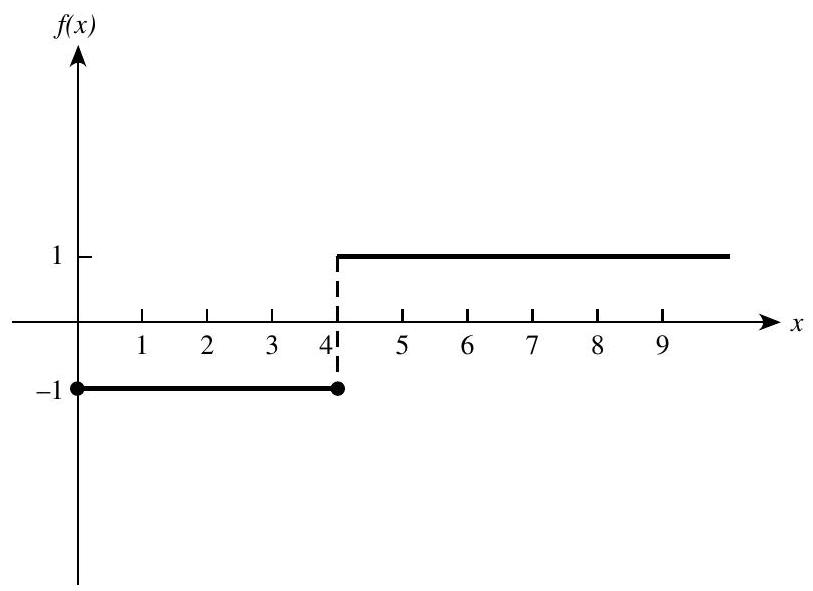
\includegraphics[max width=\textwidth]{2024_04_03_5bb5b4275a64cb9887d1g-232}
\end{center}

Fig. 21-1

$$
\begin{aligned}
\mathscr{L}\{f(x)\} & =\int_{0}^{\infty} e^{-s x} f(x) d x=\int_{0}^{4} e^{-s x}(-1) d x+\int_{4}^{\infty} e^{-s x}(1) d x \\
& =\left.\frac{e^{-s x}}{s}\right|_{x=0} ^{x=4}+\lim _{R \rightarrow \infty} \int_{4}^{R} e^{-s x} d x \\
& =\frac{e^{-4 s}}{s}-\frac{1}{s}+\lim _{R \rightarrow \infty}\left(\frac{-1}{s} e^{-R s}+\frac{1}{s} e^{-4 s}\right) \\
& =\frac{2 e^{-4 s}}{s}-\frac{1}{s} \quad(\text { for } s>0)
\end{aligned}
$$

21.10. Find the Laplace transform of $f(x)=3+2 x^{2}$.

Using Property 21.1 with the results of Problems 21.4 and 21.5 , or alternatively, entries 1 and $3(n=3)$ of Appendix A, we have

$$
\begin{aligned}
F(s) & =\mathscr{L}\left\{3+2 x^{2}\right\}=3 \mathscr{L}\{1\}+2 \mathscr{L}\left\{x^{2}\right\} \\
& =3\left(\frac{1}{s}\right)+2\left(\frac{2}{s^{3}}\right)=\frac{3}{s}+\frac{4}{s^{3}}
\end{aligned}
$$

21.11. Find the Laplace transform of $f(x)=5 \sin 3 x-17 e^{-2 x}$.

Using Property 21.1 with the results of Problems $21.6(a=-2)$ and $21.7(a=3)$, or alternatively, entries 7 and 8 of Appendix A, we have

$$
\begin{aligned}
F(s) & =\mathscr{L}\left\{5 \sin 3 x-17 e^{-2 x}\right\}=5 \mathscr{L}\{\sin 3 x\}-17 \mathscr{L}\left\{e^{-2 x}\right\} \\
& =5\left(\frac{3}{s^{2}+(3)^{2}}\right)-17\left(\frac{1}{s-(-2)}\right)=\frac{15}{s^{2}+9}-\frac{17}{s+2}
\end{aligned}
$$

21.12. Find the Laplace transform of $f(x)=2 \sin x+3 \cos 2 x$.

Using Property 21.1 with entries $8(a=1)$ and $9(a=2)$ of Appendix A, we have

$$
\begin{aligned}
F(s) & =\mathscr{L}\{2 \sin x+3 \cos 2 x\}=2 \mathscr{L}\{\sin x\}+3 \mathscr{L}\{\cos 2 x\} \\
& =2 \frac{1}{s^{2}+1}+3 \frac{s}{s^{2}+4}=\frac{2}{s^{2}+1}+\frac{3 s}{s^{2}+4}
\end{aligned}
$$

21.13. Find the Laplace transform of $f(x)=2 x^{2}-3 x+4$.

Using Property 21.1 repeatedly with entries 1,2 and $3(n=3)$ of Appendix A, we have

$$
\begin{aligned}
F(s) & =\mathscr{L}\left\{2 x^{2}-3 x+4\right\}=2 \mathscr{L}\left\{x^{2}\right\}-3 \mathscr{L}\{x\}+4 \mathscr{L}\{1\} \\
& =2\left(\frac{2}{s^{3}}\right)-3\left(\frac{1}{s^{2}}\right)+4\left(\frac{1}{s}\right)=\frac{4}{s^{3}}-\frac{3}{s^{2}}+\frac{4}{s}
\end{aligned}
$$

21.14. Find $\mathscr{L}\left\{x e^{4 x}\right\}$.

This problem can be done three ways.\\
(a) Using entry 14 of Appendix A with $n=2$ and $a=4$, we have directly that

$$
\mathscr{L}\left\{x e^{4 x}\right\}=\frac{1}{(s-4)^{2}}
$$

(b) Set $f(x)=x$. Using Property 21.2 with $a=4$ and entry 2 of Appendix A, we have

and

$$
\begin{aligned}
& F(s)=\mathscr{L}\{f(x)\}=\mathscr{L}\{x\}=\frac{1}{s^{2}} \\
& \mathscr{L}\left\{e^{4 x} x\right\}=F(s-4)=\frac{1}{(s-4)^{2}}
\end{aligned}
$$

(c) Set $f(x)=e^{4 x}$. Using Property 21.3 with $n=1$ and the results of Problem 21.6, or alternatively, entry 7 of Appendix A with $a=4$, we find that

and

$$
\begin{gathered}
F(s)=\mathscr{L}\{f(x)\}=\mathscr{L}\left\{e^{4 x}\right\}=\frac{1}{s-4} \\
\mathscr{L}\left\{x e^{4 x}\right\}=-F^{\prime}(s)=-\frac{d}{d s}\left(\frac{1}{s-4}\right)=\frac{1}{(s-4)^{2}}
\end{gathered}
$$

21.15. Find $\mathscr{L}\left\{e^{-2 x} \sin 5 x\right\}$.

This problem can be done two ways.

(a) Using entry 15 of Appendix A with $b=-2$ and $a=5$, we have directly that

$$
\mathscr{L}\left\{e^{-2 x} \sin 5 x\right\}=\frac{5}{[s-(-2)]^{2}+(5)^{2}}=\frac{5}{(s+2)^{2}+25}
$$

(b) Set $f(x)=\sin 5 x$. Using Property 21.2 with $a=-2$ and the results of Problem 21.7, or alternatively, entry 8 of Appendix A with $a=5$, we have

$$
\begin{gathered}
F(s)=\mathscr{L}\{f(x)\}=\mathscr{L}\{\sin 5 x\}=\frac{5}{s^{2}+25} \\
\mathscr{L}\left\{e^{-2 x} \sin 5 x\right\}=F(s-(-2))=F(s+2)=\frac{5}{(s+2)^{2}+25}
\end{gathered}
$$

and

21.16. Find $\mathscr{L}\{x \cos \sqrt{7} x\}$.

This problem can be done two ways.

(a) Using entry 13 of Appendix A with $a=\sqrt{7}$, we have directly that

$$
\mathscr{L}\{x \cos \sqrt{7} x\}=\frac{s^{2}-(\sqrt{7})^{2}}{\left[s^{2}+(\sqrt{7})^{2}\right]^{2}}=\frac{s^{2}-7}{\left(s^{2}+7\right)^{2}}
$$

(b) Set $f(x)=\cos \sqrt{7} x$. Using Property 21.3 with $n=1$ and entry 9 of Appendix A with $a=\sqrt{7}$, we have

$$
F(s)=\mathscr{L}\{\cos \sqrt{7} x\}=\frac{s}{s^{2}+(\sqrt{7})^{2}}=\frac{s}{s^{2}+7}
$$

and

$$
\mathscr{L}\{x \cos \sqrt{7} x\}=-\frac{d}{d s}\left(\frac{s}{s^{2}+7}\right)=\frac{s^{2}-7}{\left(s^{2}+7\right)^{2}}
$$

21.17. Find $\mathscr{L}\left\{e^{-x} x \cos 2 x\right\}$.

Let $f(x)=x \cos 2 x$. From entry 13 of Appendix A with $a=2$, we obtain

$$
F(s)=\frac{s^{2}-4}{\left(s^{2}+4\right)^{2}}
$$

Then, from Property 21.2 with $a=-1$,

$$
\mathscr{L}\left\{e^{-x} x \cos 2 x\right\}=F(s+1)=\frac{(s+1)^{2}-4}{\left[(s+1)^{2}+4\right]^{2}}
$$

21.18. Find $\mathscr{L}\left\{x^{7 / 2}\right\}$.

Define $f(x)=\sqrt{x}$. Then $x^{7 / 2}=x^{3} \sqrt{x}=x^{3} f(x)$ and, from entry 4 of Appendix A, we obtain

$$
F(s)=\mathscr{L}\{f(x)\}=\mathscr{L}\{\sqrt{x}\}=\frac{1}{2} \sqrt{\pi} s^{-3 / 2}
$$

It now follows from Property 21.3 with $n=3$ that

$$
\mathscr{L}\left\{x^{3} \sqrt{x}\right\}=(-1)^{3} \frac{d^{3}}{d s^{3}}\left(\frac{1}{2} \sqrt{\pi} s^{-3 / 2}\right)=\frac{105}{16} \sqrt{\pi} s^{-9 / 2}
$$

which agrees with entry 6 of Appendix A for $n=4$.

21.19. Find $\mathscr{L}\left\{\frac{\sin 3 x}{x}\right\}$.

Taking $f(x)=\sin 3 x$, we find from entry 8 of Appendix A with $a=3$ that

$$
F(s)=\frac{3}{s^{2}+9} \quad \text { or } \quad F(t)=\frac{3}{t^{2}+9}
$$

Then, using Property 21.4 , we obtain

$$
\begin{aligned}
\mathscr{L}\left\{\frac{\sin 3 x}{x}\right\} & =\int_{s}^{\infty} \frac{3}{t^{2}+9} d t=\lim _{R \rightarrow \infty} \int_{s}^{R} \frac{3}{t^{2}+9} d t \\
& =\left.\lim _{R \rightarrow \infty} \arctan \frac{t}{3}\right|_{s} ^{R} \\
& =\lim _{R \rightarrow \infty}\left(\arctan \frac{R}{3}-\arctan \frac{s}{3}\right) \\
& =\frac{\pi}{2}-\arctan \frac{s}{3}
\end{aligned}
$$

21.20. Find $\mathscr{L}\left\{\int_{0}^{x} \sinh 2 t d t\right\}$.

Taking $f(t)=\sinh 2 t$, we have $f(x)=\sinh 2 x$. It now follows from entry 10 of Appendix A with $a=2$ that\\
$F(s)=2 /\left(s^{2}-4\right)$, and then, from Property 21.5 that

$$
\mathscr{L}\left\{\int_{0}^{x} \sinh 2 t d t\right\}=\frac{1}{s}\left(\frac{2}{s^{2}-4}\right)=\frac{2}{s\left(s^{2}-4\right)}
$$

21.21. Prove that if $f(x+\omega)=-f(x)$, then


\begin{equation*}
\mathscr{L}\{f(x)\}=\frac{\int_{0}^{\omega} e^{-s x} f(x) d x}{1+e^{-\omega s}} \tag{1}
\end{equation*}


Since

$$
f(x+2 \omega)=f[(x+\omega)+\omega]=-f(x+\omega)=-[-f(x)]=f(x)
$$

$f(x)$ is periodic with period $2 \omega$. Then, using Property 21.6 with $\omega$ replaced by $2 \omega$, we have

$$
\mathscr{L}\{f(x)\}=\frac{\int_{0}^{2 \omega} e^{-s x} f(x) d x}{1-e^{-2 \omega s}}=\frac{\int_{0}^{\omega} e^{-s x} f(x) d x+\int_{\omega}^{2 \omega} e^{-s x} f(x) d x}{1-e^{-2 \omega s}}
$$

Substituting $y=x-\omega$ into the second integral, we find that

$$
\begin{aligned}
\int_{\omega}^{2 \omega} e^{-s x} f(x) d x & =\int_{0}^{\omega} e^{-s(y+\omega)} f(y+\omega) d y=e^{-\omega s} \int_{0}^{\omega} e^{-s y}[-f(y)] d y \\
& =-e^{-\omega s} \int_{0}^{\omega} e^{-s y} f(y) d y
\end{aligned}
$$

The last integral, upon changing the dummy variable of integration back to $x$, equals

Thus,

$$
\begin{aligned}
&-e^{-\omega s} \int_{0}^{\omega} e^{-s x} f(x) d x \\
& \mathscr{L}\{f(x)\}=\frac{\left(1-e^{-\omega s}\right) \int_{0}^{\omega} e^{-s x} f(x) d x}{1-e^{-2 \omega s}} \\
&=\frac{\left(1-e^{-\omega s}\right) \int_{0}^{\omega} e^{-s x} f(x) d x}{\left(1-e^{-\omega s}\right)\left(1+e^{-\omega s}\right)}=\frac{\int_{0}^{\omega} e^{-s x} f(x) d x}{1+e^{-\omega s}}
\end{aligned}
$$

\begin{center}
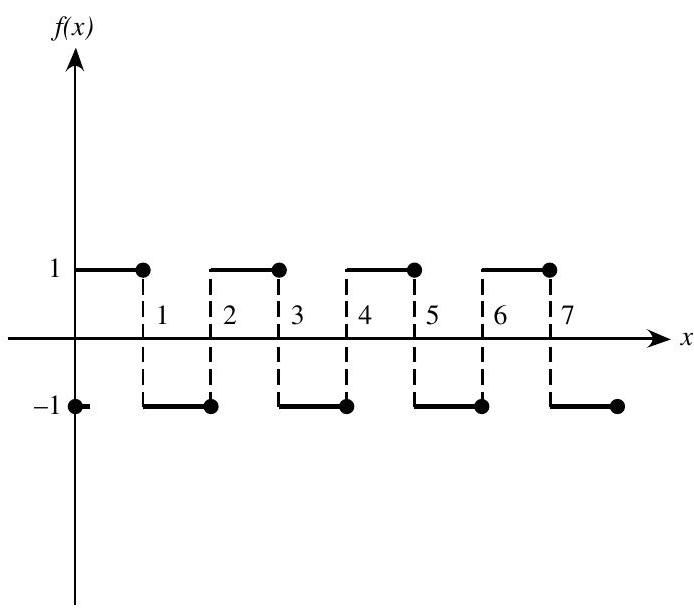
\includegraphics[max width=\textwidth]{2024_04_03_5bb5b4275a64cb9887d1g-236}
\end{center}

Fig. 21-2

21.22. Find $\mathscr{L}\{f(x)\}$ for the square wave shown in Fig. 21-2.

This problem can be done two ways.

(a) Note that $f(x)$ is periodic with period $\omega=2$, and in the interval $0<x \leq 2$ it can be defined analytically by

$$
f(x)=\left\{\begin{array}{rr}
1 & 0<x \leq 1 \\
-1 & 1<x \leq 2
\end{array}\right.
$$

From Eq. (21.8), we have

$$
\mathscr{L}\{f(x)\}=\frac{\int_{0}^{2} e^{-s x} f(x) d x}{1-e^{-2 s}}
$$

Since

$$
\begin{aligned}
\int_{0}^{2} e^{-s x} f(x) d x & =\int_{0}^{1} e^{-s x}(1) d x+\int_{1}^{2} e^{-s x}(-1) d x \\
& =\frac{1}{s}\left(e^{-2 s}-2 e^{-s}+1\right)=\frac{1}{s}\left(e^{-s}-1\right)^{2}
\end{aligned}
$$

it follows that

$$
\begin{aligned}
F(s) & =\frac{\left(e^{-s}-1\right)^{2}}{s\left(1-e^{-2 s}\right)}=\frac{\left(1-e^{-s}\right)^{2}}{s\left(1-e^{-s}\right)\left(1+e^{-s}\right)}=\frac{1-e^{-s}}{s\left(1+e^{-s}\right)} \\
& =\left[\frac{e^{s / 2}}{e^{s / 2}}\right]\left[\frac{1-e^{-s}}{s\left(1+e^{-s}\right)}\right]=\frac{e^{s / 2}-e^{-s / 2}}{s\left(e^{s / 2}+e^{-s / 2}\right)}=\frac{1}{s} \tanh \frac{s}{2}
\end{aligned}
$$

(b) The square wave $f(x)$ also satisfies the equation $f(x+1)=-f(x)$. Thus, using ( 1 ) of Problem 21.21 with $\omega=1$, we obtain

$$
\begin{aligned}
\mathscr{L}\{f(x)\} & =\frac{\int_{0}^{1} e^{-s x} f(x) d x}{1+e^{-s}}=\frac{\int_{0}^{1} e^{-s x}(1) d x}{1+e^{-s}} \\
& =\frac{(1 / s)\left(1-e^{-s}\right)}{1+e^{-s}}=\frac{1}{s} \tanh \frac{s}{2}
\end{aligned}
$$

\begin{center}
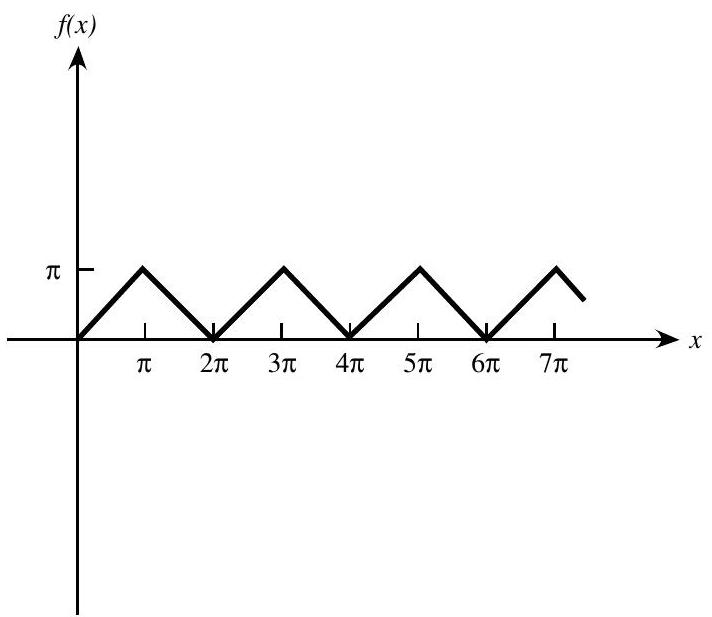
\includegraphics[max width=\textwidth]{2024_04_03_5bb5b4275a64cb9887d1g-237}
\end{center}

Fig. 21-3

21.23. Find the Laplace transform of the function graphed in Fig. 21-3.

Note that $f(x)$ is periodic with period $\omega=2 \pi$, and in the interval $0 \leq x<2 \pi$ it can be defined analytically by

$$
f(x)=\left\{\begin{array}{cc}
x & 0 \leq x \leq \pi \\
2 \pi-x & \pi \leq x<2 \pi
\end{array}\right.
$$

From Eq. (21.8), we have

$$
\mathscr{L}\{f(x)\}=\frac{\int_{0}^{2 \pi} e^{-s x} f(x) d x}{1-e^{-2 \pi s}}
$$

Since

$$
\begin{aligned}
\int_{0}^{2 \pi} e^{-s x} f(x) d x & =\int_{0}^{\pi} e^{-s x} x d x+\int_{0}^{2 \pi} e^{-s x}(2 \pi-x) d x \\
& =\frac{1}{s^{2}}\left(e^{-2 \pi s}-2 e^{-\pi s}+1\right)=\frac{1}{s^{2}}\left(e^{-\pi s}-1\right)^{2}
\end{aligned}
$$

it follows that

$$
\begin{aligned}
\mathscr{L}\{f(x)\} & =\frac{\left(1 / s^{2}\right)\left(e^{-\pi s}-1\right)^{2}}{1-e^{-2 \pi s}}=\frac{\left(1 / s^{2}\right)\left(e^{-\pi s}-1\right)^{2}}{\left(1-e^{-\pi s}\right)\left(1+e^{-\pi s}\right)} \\
& =\frac{1}{s^{2}}\left(\frac{1-e^{-\pi s}}{1+e^{-\pi s}}\right)=\frac{1}{s^{2}} \tanh \frac{\pi s}{2}
\end{aligned}
$$

21.24. Find $\mathscr{L}\left\{e^{4 x} x \int_{0}^{x} \frac{1}{t} e^{-4 t} \sin 3 t d t\right\}$.

Using Eq. (21.4) with $a=-4$ on the results of Problem 21.19, we obtain

$$
\mathscr{L}\left\{\frac{1}{x} e^{-4 x} \sin 3 x\right\}=\frac{\pi}{2}-\arctan \frac{s+4}{3}
$$

It now follows from Eq. (21.7) that

$$
\mathscr{L}\left\{\int_{0}^{x} \frac{1}{t} e^{-4 t} \sin 3 t d t\right\}=\frac{\pi}{2 s}-\frac{1}{s} \arctan \frac{s+4}{3}
$$

and then from Property 21.3 with $n=1$,

$$
\mathscr{L}\left\{x \int_{0}^{x} \frac{1}{t} e^{-4 t} \sin 3 t d t\right\}=\frac{\pi}{2 s^{2}}-\frac{1}{s^{2}} \arctan \frac{s+4}{3}+\frac{3}{s\left[9+(s+4)^{2}\right]}
$$

Finally, using Eq. (21.4) with $a=4$, we conclude that the required transform is

$$
\frac{\pi}{2(s-4)^{2}}-\frac{1}{(s-4)^{2}} \arctan \frac{s}{3}+\frac{3}{(s-4)\left(s^{2}+9\right)}
$$

21.25. Find the Laplace transforms at $(a) t,(b) e^{a t}$, and $(c)$ sin $a t$, where $a$ denotes a constant.

Using entries 2, 7, and 8 of Appendix A with $x$ replaced by $t$, we find the Laplace transforms to be,\\
respectively,\\
(a) $\mathscr{L}\{t\}=\frac{1}{s^{2}}$\\
(b) $\mathscr{L}\left\{e^{a t}\right\}=\frac{1}{s-a}$\\
(c) $\mathscr{L}\{\sin a t\}=\frac{a}{s^{2}+a^{2}}$

21.26. Find the Laplace transforms of $(a) \theta^{2},(b) \cos a \theta,(c) e^{b \theta} \sin a \theta$, where $a$ and $b$ denote constants.

Using entries 3 (with $n=3$ ), 9, and 15 of Appendix A with $x$ replaced by $\theta$, we find the Laplace transforms to be, respectively.\\
(a) $\mathscr{L}\left\{\theta^{2}\right\}=\frac{2}{s^{3}}$\\
(b) $\mathscr{L}\{\cos a \theta\}=\frac{s}{s^{2}+a^{2}}$\\
(c) $\mathscr{L}\left\{e^{b \theta} \sin a \theta\right\}=\frac{a}{(s-b)^{2}+a^{2}}$

\section*{Supplementary Problems}
In Problems 21.27 and 21.42, find the Laplace transforms of the given function using Eq. (21.1).

21.27. $f(x)=3$

21.29. $f(x)=e^{2 x}$

21.31. $f(x)=x$

21.33. $f(x)=\cos 3 x$

21.35. $f(x)=\cos b x$, where $b$ denotes a constant

21.37. $f(x)=x e^{b x}$, where $b$ denotes a constant

21.39. $f(x)=\left\{\begin{array}{rr}x & 0 \leq x \leq 2 \\ 2 & x>2\end{array}\right.$

21.41. $f(x)$ in Fig. $21-4$\\
21.28. $f(x)=\sqrt{5}$

21.30. $f(x)=e^{-6 x}$

21.32. $f(x)=-8 x$

21.34. $f(x)=\cos 4 x$

21.36. $f(x)=x e^{-8 x}$

21.38. $f(x)=x^{3}$

21.40. $f(x)=\left\{\begin{array}{rr}1 & 0 \leq x \leq 1 \\ e^{x} & 1<x \leq 4 \\ 0 & x>4\end{array}\right.$

21.42. $f(x)$ in Fig. $21-5$

In Problems 21.43 and 21.76, use Appendix A and the Properties 21.1 through 21.6, where appropriate, to find the Laplace transforms of the given functions.

\begin{center}
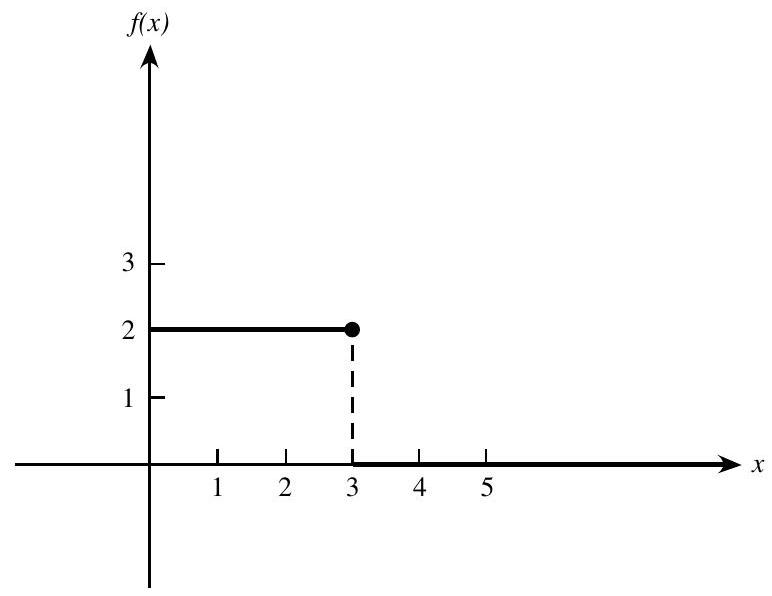
\includegraphics[max width=\textwidth]{2024_04_03_5bb5b4275a64cb9887d1g-239}
\end{center}

Fig. 21-4

\begin{center}
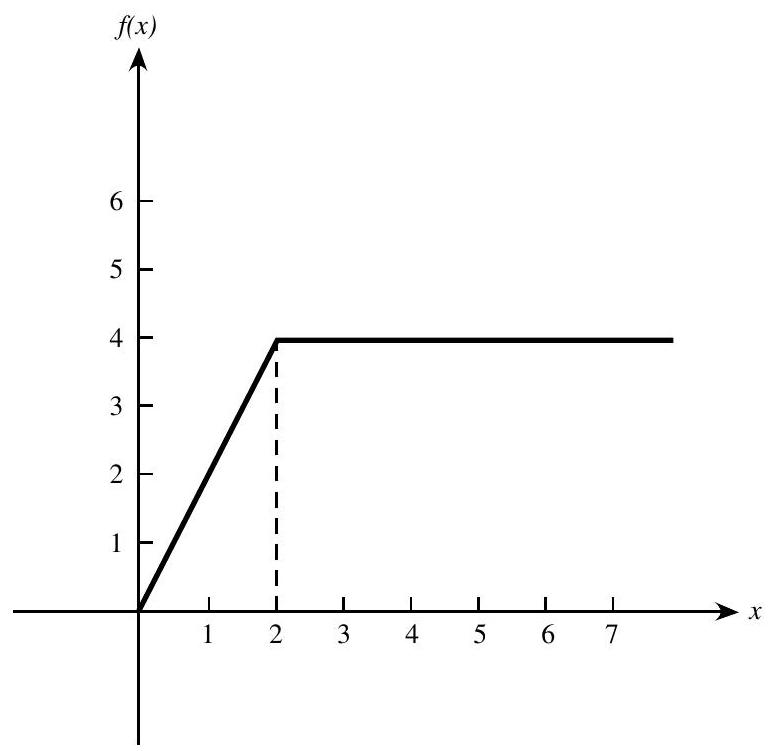
\includegraphics[max width=\textwidth]{2024_04_03_5bb5b4275a64cb9887d1g-240}
\end{center}

Fig. 21-5

21.43. $f(x)=x^{7}$

21.45. $f(x)=x^{5} e^{-x}$

21.47. $f(x)=\frac{1}{3} e^{-x / 3}$

21.49. $f(x)=2 \sin ^{2} \sqrt{3} x$

21.51. $f(x)=3 \sin \frac{x}{2}$

21.53. $f(x)=-\frac{9}{5} \sqrt{x}$

21.55. $f(x)=e^{x} \sin 2 x$

21.57. $f(x)=e^{3 x} \cos 2 x$

21.59. $f(x)=e^{5 x} \sqrt{x}$

21.61. $f(x)=e^{-2 x} \sin ^{2} x$

21.63. $5 e^{2 x}+7 e^{-x}$

21.65. $f(x)=3-4 x^{2}$

21.67. $f(x)=2 \cos 3 x-\sin 3 x$

21.69. $2 x^{2} e^{-x} \cosh x$

21.71. $\sqrt{x} e^{2 x}$

21.73. $\int_{0}^{x} e^{3 t} \cos t d t$

21.75. $f(x)$ in Fig. $21-7$\\
21.44. $f(x)=x \cos 3 x$

21.46. $f(x)=\frac{1}{\sqrt{x}}$

21.48. $f(x)=5 e^{-x / 3}$

21.50. $f(x)=8 e^{-5 x}$

21.52. $f(x)=-\cos \sqrt{19} x$

21.54. $f(x)=e^{-x} \sin 2 x$

21.56. $f(x)=e^{-x} \cos 2 x$

21.58. $f(x)=e^{3 x} \cos 5 x$

21.60. $f(x)=e^{-5 x} \sqrt{x}$

21.62. $x^{3}+3 \cos 2 x$

21.64. $f(x)=2+3 x$

21.66. $f(x)=2 x+5 \sin 3 x$

21.68. $2 x^{2} \cosh x$

21.70. $x^{2} \sin 4 x$

21.72. $\int_{0}^{x} t \sinh t d t$

21.74. $f(x)$ in Fig. 21-6

21.76. $f(x)$ in Fig. $21-8$

\begin{center}
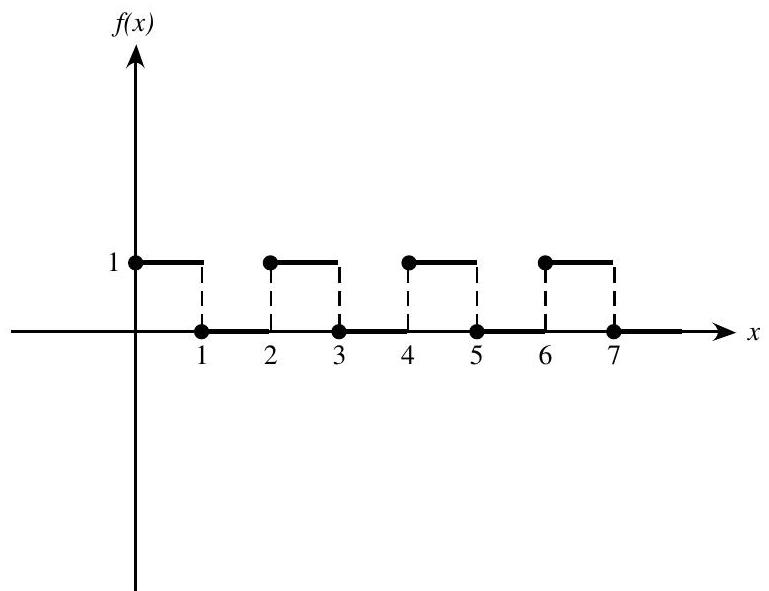
\includegraphics[max width=\textwidth]{2024_04_03_5bb5b4275a64cb9887d1g-241(2)}
\end{center}

Fig. 21-6

\begin{center}
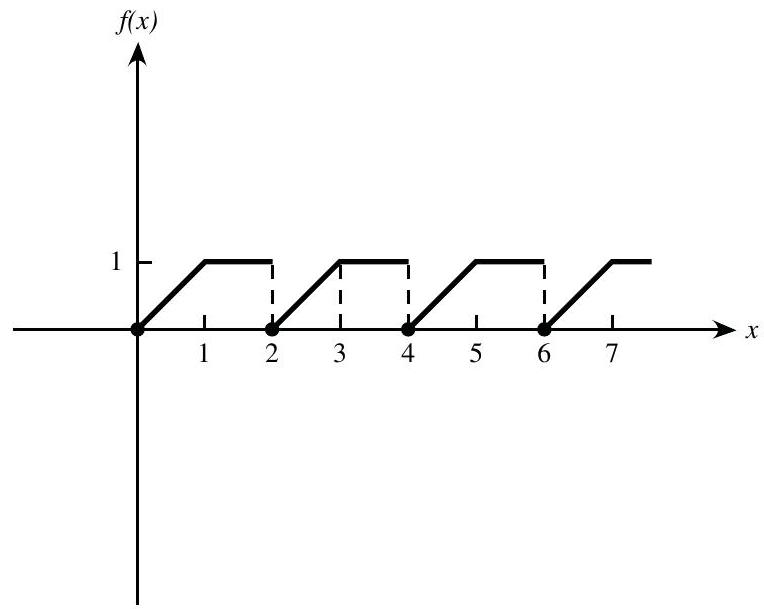
\includegraphics[max width=\textwidth]{2024_04_03_5bb5b4275a64cb9887d1g-241}
\end{center}

Fig. 21-7

\begin{center}
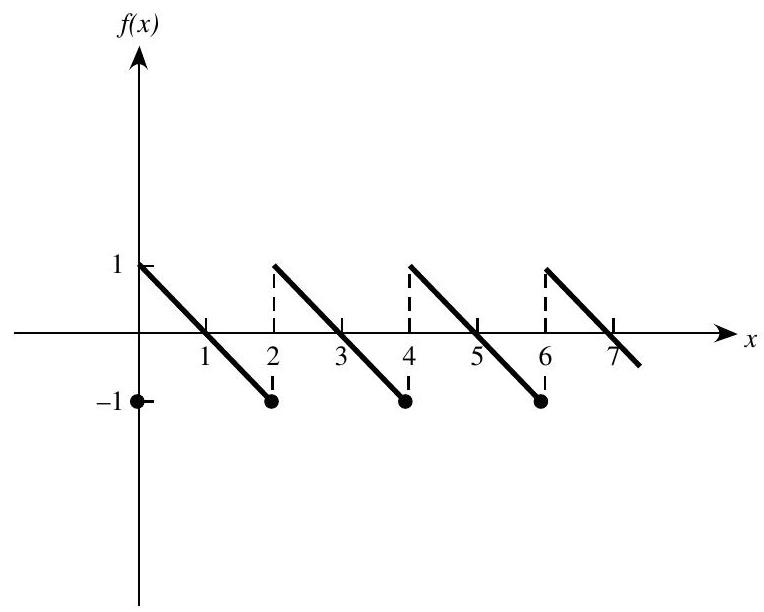
\includegraphics[max width=\textwidth]{2024_04_03_5bb5b4275a64cb9887d1g-241(1)}
\end{center}

Fig. 21-8

\section*{CHAPTER 22}
\section*{Inverse Laplace Transforms}
\section*{DEFINITION}
An inverse Laplace transform of $F(s)$, designated by $\mathscr{L}^{-1}\{F(s)\}$, is another function $f(x)$ having the property that $\mathscr{L}\{f(x)\}=F(s)$. This presumes that the independent variable of interest is $x$. If the independent variable of interest is $t$ instead, then an inverse Laplace transform of $F(s)$ if $f(t)$ where $\mathscr{L}\{f(t)\}=F(s)$.

The simplest technique for identifying inverse Laplace transforms is to recognize them, either from memory or from a table such as Appendix A (see Problems 22.1 through 22.3). If $F(s)$ is not in a recognizable form, then occasionally it can be transformed into such a form by algebraic manipulation. Observe from Appendix A that almost all Laplace transforms are quotients. The recommended procedure is to first convert the denominator to a form that appears in Appendix A and then the numerator.

\section*{MANIPULATING DENOMINATORS}
The method of completing the square converts a quadratic polynomial into the sum of squares, a form that appears in many of the denominators in Appendix A. In particular, for the quadratic $a s^{2}+b s+c$, where $a, b$, and $c$ denote constants,

$$
\begin{aligned}
a s^{2}+b s+c & =a\left(s^{2}+\frac{b}{a} s\right)+c \\
& =a\left[s^{2}+\frac{b}{a} s+\left(\frac{b}{2 a}\right)^{2}\right]+\left[c-\frac{b^{2}}{4 a}\right] \\
& =a\left(s+\frac{b}{2 a}\right)^{2}+\left(c-\frac{b^{2}}{4 a}\right) \\
& =a(s+k)^{2}+h^{2}
\end{aligned}
$$

where $k=b / 2 a$ and $h=\sqrt{c-\left(b^{2} / 4 a\right)}$. (See Problems 22.8 through 22.10.)

The method of partial fractions transforms a function of the form $a(s) / b(s)$, where both $a(s)$ and $b(s)$ are polynomials in $s$, into the sum of other fractions such that the denominator of each new fraction is either a firstdegree or a quadratic polynomial raised to some power. The method requires only that (1) the degree of $a(s)$ be less than the degree of $b(s)$ (if this is not the case, first perform long division, and consider the remainder term) and (2) $b(s)$ be factored into the product of distinct linear and quadratic polynomials raised to various powers.

The method is carried out as follows. To each factor of $b(s)$ of the form $(s-a)^{m}$, assign a sum of $m$ fractions, of the form

$$
\frac{A_{1}}{s-a}+\frac{A_{2}}{(s-a)^{2}}+\cdots+\frac{A_{m}}{(s-a)^{m}}
$$

To each factor of $b(s)$ of the form $\left(s^{2}+b s+c\right)^{p}$, assign a sum of $p$ fractions, of the form

$$
\frac{B_{1} s+C_{1}}{s^{2}+b s+c}+\frac{B_{2} s+C_{2}}{\left(s^{2}+b s+c\right)^{2}}+\cdots+\frac{B_{p} s+C_{p}}{\left(s^{2}+b s+c\right)^{p}}
$$

Here $A_{i}, B_{j}$, and $C_{k}(i=1,2, \ldots, m ; j, k=1,2, \ldots, p)$ are constants which still must be determined.

Set the original fraction $a(s) / b(s)$ equal to the sum of the new fractions just constructed. Clear the resulting equation of fractions and then equate coefficients of like powers of $s$, thereby obtaining a set of simultaneous linear equations in the unknown constants $A_{i}, B_{j}$, and $C_{k}$. Finally, solve these equations for $A_{i}, B_{j}$, and $C_{k}$. (See Problems 22.11 through 22.14.)

\section*{MANIPULATING NUMERATORS}
A factor $s-a$ in the numerators may be written in terms of the factor $s-b$, where both $a$ and $b$ are constants, through the identity $s-a=(s-b)+(b-a)$. The multiplicative constant $a$ in the numerator may be written explicitly in terms of the multiplicative constant $b$ through the identity

$$
a=\frac{a}{b}(b)
$$

Both identities generate recognizable inverse Laplace transforms when they are combined with:

Property 22.1. (Linearity). If the inverse Laplace transforms of two functions $F(s)$ and $G(s)$ exist, then for any constants $c_{1}$ and $c_{2}$,

$$
\mathscr{L}^{-1}\left\{c_{1} F(s)+c_{2} G(s)\right\}=c_{1} \mathscr{L}^{-1}\{F(s)\}+c_{2} \mathscr{L}^{-1}\{G(s)\}
$$

(See Problems 22.4 through 22.7.)

\section*{Solved Problems}
22.1. Find $\mathscr{L}^{-1}\left\{\frac{1}{s}\right\}$.

Here $F(s)=1 / s$. From either Problem 21.4 or entry 1 of Appendix A, we have $\mathscr{L}\{1\}=1 / s$. Therefore, $\mathscr{L}^{-1}\{1 / s\}=1$.

22.2. Find $\mathscr{L}^{-1}\left\{\frac{1}{s-8}\right\}$.

From either Problem 21.6 or entry 7 of Appendix A with $a=8$, we have

$$
\mathscr{L}\left\{e^{8 x}\right\}=\frac{1}{s-8}
$$

Therefore,

$$
\mathscr{L}^{-1}\left\{\frac{1}{s-8}\right\}=e^{8 x}
$$

22.3. Find $\mathscr{L}^{-1}\left\{\frac{s}{s^{2}+6}\right\}$.

From entry 9 of Appendix A with $a=\sqrt{6}$, we have

Therefore,

$$
\begin{gathered}
\mathscr{L}\{\cos \sqrt{6} x\}=\frac{s}{s^{2}+(\sqrt{6})^{2}}=\frac{s}{s^{2}+6} \\
\mathscr{L}^{-1}\left\{\frac{s}{s^{2}+6}\right\}=\cos \sqrt{6} x
\end{gathered}
$$

22.4. Find $\mathscr{L}^{-1}\left\{\frac{5 s}{\left(s^{2}+1\right)^{2}}\right\}$.

The given function is similar in form to entry 12 of Appendix A. The denominators become identical if we take $a=1$. Manipulating the numerator of the given function and using Property 22.1, we obtain

$$
\mathscr{L}^{-1}\left\{\frac{5 s}{\left(s^{2}+1\right)^{2}}\right\}=\mathscr{L}^{-1}\left\{\frac{\frac{5}{2}(2 s)}{\left(s^{2}+1\right)^{2}}\right\}=\frac{5}{2} \mathscr{L}^{-1}\left\{\frac{2 s}{\left(s^{2}+1\right)^{2}}\right\}=\frac{5}{2} x \sin x
$$

22.5. Find $\mathscr{L}^{-1}\left\{\frac{1}{\sqrt{s}}\right\}$.

The given function is similar in form to entry 5 of Appendix A. Their denominators are identical; manipulating the numerator of the given function and using Property 22.1, we obtain

$$
\mathscr{L}^{-1}\left\{\frac{1}{\sqrt{s}}\right\}=\mathscr{L}^{-1}\left\{\frac{1}{\sqrt{\pi}} \frac{\sqrt{\pi}}{\sqrt{s}}\right\}=\frac{1}{\sqrt{\pi}} \mathscr{L}^{-1}\left\{\frac{\sqrt{\pi}}{\sqrt{s}}\right\}=\frac{1}{\sqrt{\pi}} \frac{1}{\sqrt{x}}
$$

22.6. Find $\mathscr{L}^{-1}\left\{\frac{s+1}{s^{2}-9}\right\}$.

The denominator of this function is identical to the denominator of entries 10 and 11 of Appendix A with $a=3$. Using Property 22.1 followed by a simple algebraic manipulation, we obtain

$$
\begin{aligned}
\mathscr{L}^{-1}\left\{\frac{s+1}{s^{2}-9}\right\} & =\mathscr{L}^{-1}\left\{\frac{s}{s^{2}-9}\right\}+\mathscr{L}^{-1}\left\{\frac{1}{s^{2}-9}\right\}=\cosh 3 x+\mathscr{L}^{-1}\left\{\frac{1}{3}\left(\frac{3}{s^{2}-(3)^{2}}\right)\right\} \\
& =\cosh 3 x+\frac{1}{3} \mathscr{L}^{-1}\left\{\frac{3}{s^{2}-(3)^{2}}\right\}=\cosh 3 x+\frac{1}{3} \sinh 3 x
\end{aligned}
$$

22.7. Find $\mathscr{L}^{-1}\left\{\frac{s}{(s-2)^{2}+9}\right\}$.

The denominator of this function is identical to the denominators of entries 15 and 16 of Appendix A with $a=3$ and $b=2$. Both the given function and entry 16 have the variable $s$ in their numerators, so they are the most closely matched. Manipulating the numerator of the given function and using Property 22.1, we obtain

$$
\begin{aligned}
\mathscr{L}^{-1}\left\{\frac{s}{(s-2)^{2}+9}\right\} & =\mathscr{L}^{-1}\left\{\frac{(s-2)+2}{(s-2)^{2}+9}\right\}=\mathscr{L}^{-1}\left\{\frac{s-2}{(s-2)^{2}+9}\right\}+\mathscr{L}^{-1}\left\{\frac{2}{(s-2)^{2}+9}\right\} \\
& =e^{2 x} \cos 3 x+\mathscr{L}^{-1}\left\{\frac{2}{(s-2)^{2}+9}\right\}=e^{2 x} \cos 3 x+\mathscr{L}^{-1}\left\{\frac{2}{3}\left(\frac{3}{(s-2)^{2}+9}\right)\right\} \\
& =e^{2 x} \cos 3 x+\frac{2}{3} \mathscr{L}^{-1}\left\{\frac{3}{(s-2)^{2}+9}\right\}=e^{2 x} \cos 3 x+\frac{2}{3} e^{2 x} \sin 3 x
\end{aligned}
$$

22.8. Find $\mathscr{L}^{-1}\left\{\frac{1}{s^{2}-2 s+9}\right\}$.

No function of this form appears in Appendix A. But, by completing the square, we obtain

$$
s^{2}-2 s+9=\left(s^{2}-2 s+1\right)+(9-1)=(s-1)^{2}+(\sqrt{8})^{2}
$$

Hence,

$$
\frac{1}{s^{2}-2 s+9}=\frac{1}{(s-1)^{2}+(\sqrt{8})^{2}}=\left(\frac{1}{\sqrt{8}}\right) \frac{\sqrt{8}}{(s-1)^{2}+(\sqrt{8})^{2}}
$$

Then, using Property 22.1 and entry 15 of Appendix A with $a=\sqrt{8}$ and $b=1$, we find that

$$
\mathscr{L}^{-1}\left\{\frac{1}{s^{2}-2 s+9}\right\}=\frac{1}{\sqrt{8}} \mathscr{L}^{-1}\left\{\frac{\sqrt{8}}{(s-1)^{2}+(\sqrt{8})^{2}}\right\}=\frac{1}{\sqrt{8}} e^{x} \sin \sqrt{8} x
$$

22.9. Find $\mathscr{L}^{-1}\left\{\frac{s+4}{s^{2}+4 s+8}\right\}$.

No function of this form appears in Appendix A. Completing the square in the denominator, we have

$$
s^{2}+4 s+8=\left(s^{2}+4 s+4\right)+(8-4)=(s+2)^{2}+(2)^{2}
$$

Hence,

$$
\frac{s+4}{s^{2}+4 s+8}=\frac{s+4}{(s+2)^{2}+(2)^{2}}
$$

This expression also is not found in Appendix A. However, if we rewrite the numerator as $s+4=(s+2)+2$ and then decompose the fraction, we have

$$
\frac{s+4}{s^{2}+4 s+8}=\frac{s+2}{(s+2)^{2}+(2)^{2}}+\frac{2}{(s+2)^{2}+(2)^{2}}
$$

Then, from entries 15 and 16 of Appendix A,

$$
\begin{aligned}
\mathscr{L}^{-1}\left\{\frac{s+4}{s^{2}+4 s+8}\right\} & =\mathscr{L}^{-1}\left\{\frac{s+2}{(s+2)^{2}+(2)^{2}}\right\}+\mathscr{L}^{-1}\left\{\frac{2}{(s+2)^{2}+(2)^{2}}\right\} \\
& =e^{-2 x} \cos 2 x+e^{-2 x} \sin 2 x
\end{aligned}
$$

22.10. Find $\mathscr{L}^{-1}\left\{\frac{s+2}{s^{2}-3 s+4}\right\}$.

No function of this form appears in Appendix A. Completing the square in the denominator, we obtain

$$
s^{2}-3 s+4=\left(s^{2}-3 s+\frac{9}{4}\right)+\left(4-\frac{9}{4}\right)=\left(s-\frac{3}{2}\right)^{2}+\left(\frac{\sqrt{7}}{2}\right)^{2}
$$

so that

$$
\frac{s+2}{s^{2}-3 s+4}=\frac{s+2}{\left(s-\frac{3}{2}\right)^{2}+\left(\frac{\sqrt{7}}{2}\right)^{2}}
$$

We now rewrite the numerator as

$$
s+2=s-\frac{3}{2}+\frac{7}{2}=\left(s-\frac{3}{2}\right)+\sqrt{7}\left(\frac{\sqrt{7}}{2}\right)
$$

so that

$$
\frac{s+2}{s^{2}-3 s+4}=\frac{s-\frac{3}{2}}{\left(s-\frac{3}{2}\right)^{2}+\left(\frac{\sqrt{7}}{2}\right)^{2}}+\sqrt{7} \frac{\frac{\sqrt{7}}{2}}{\left(s-\frac{3}{2}\right)^{2}+\left(\frac{\sqrt{7}}{2}\right)^{2}}
$$

Then,

$$
\begin{aligned}
\mathscr{L}^{-1}\left\{\frac{s+2}{s^{2}-3 s+4}\right\} & =\mathscr{L}^{-1}\left\{\frac{s-\frac{3}{2}}{\left(s-\frac{3}{2}\right)^{2}+\left(\frac{\sqrt{7}}{2}\right)^{2}}\right\}+\sqrt{7} \mathscr{L}^{-1}\left\{\frac{\frac{\sqrt{7}}{2}}{\left(s-\frac{3}{2}\right)^{2}+\left(\frac{\sqrt{7}}{2}\right)^{2}}\right\} \\
& =e^{(3 / 2) x} \cos \frac{\sqrt{7}}{2} x+\sqrt{7} e^{(3 / 2) x} \sin \frac{\sqrt{7}}{2} x
\end{aligned}
$$

22.11. Use partial function to decompose $\frac{1}{(s+1)\left(s^{2}+1\right)}$.

To the linear factor $s+1$, we associate the fraction $A /(s+1)$; whereas to the quadratic factor $s^{2}+1$, we associate the fraction $(B s+C) /\left(s^{2}+1\right)$. We then set


\begin{equation*}
\frac{1}{(s+1)\left(s^{2}+1\right)} \equiv \frac{A}{s+1}+\frac{B s+C}{s^{2}+1} \tag{1}
\end{equation*}


Clearing fractions, we obtain


\begin{equation*}
1 \equiv A\left(s^{2}+1\right)+(B s+C)(s+1) \tag{2}
\end{equation*}


or

$$
s^{2}(0)+s(0)+1 \equiv s^{2}(A+B)+s(B+C)+(A+C)
$$

Equating coefficients of like powers of $s$, we conclude that $A+B=0, B+C=0$, and $A+C=1$. The solution of this set of equations is $A=\frac{1}{2}, B=-\frac{1}{2}$, and $C=\frac{1}{2}$. Substituting these values into (1), we obtain the partial-fractions decomposition

$$
\frac{1}{(s+1)\left(s^{2}+1\right)} \equiv \frac{\frac{1}{2}}{s+1}+\frac{-\frac{1}{2} s+\frac{1}{2}}{s^{2}+1}
$$

The following is an alternative procedure for finding the constants $A, B$, and $C$ in (1). Since (2) must hold for all $s$, it must in particular hold $s=-1$. Substituting this value into (2), we immediately find $A=\frac{1}{2}$. Equation (2) must also hold for $s=0$. Substituting this value along with $A=\frac{1}{2}$ into (2), we obtain $C=\frac{1}{2}$. Finally, substituting any other value of $s$ into (2), we find that $B=-\frac{1}{2}$.

22.12. Use partial fractions to decompose $\frac{1}{\left(s^{2}+1\right)\left(s^{2}+4 s+8\right)}$.

To the quadratic factors $s^{2}+1$ and $s^{2}+4 s+8$, we associate the fractions $(A s+B) /\left(s^{2}+1\right)$ and $(C s+D) /\left(s^{2}+4 s+8\right)$. We set


\begin{equation*}
\frac{1}{\left(s^{2}+1\right)\left(s^{2}+4 s+8\right)} \equiv \frac{A s+B}{s^{2}+1}+\frac{C s+D}{s^{2}+4 s+8} \tag{1}
\end{equation*}


and clear fractions to obtain

or

$$
\begin{gathered}
1 \equiv(A s+B)\left(s^{2}+4 s+8\right)+(C s+D)\left(s^{2}+1\right) \\
s^{3}(0)+s^{2}(0)+s(0)+1 \equiv s^{3}(A+C)+s^{2}(4 A+B+D)+s(8 A+4 B+C)+(8 B+D)
\end{gathered}
$$

Equating coefficients of like powers of $s$, we obtain $A+C=0,4 A+B+D=0,8 A+4 B+C=0$, and $8 B+D=1$. The solution of this set of equation is

$$
A=-\frac{4}{65} \quad B=\frac{7}{65} \quad C=\frac{4}{65} \quad D=\frac{9}{65}
$$

Therefore,

$$
\frac{1}{\left(s^{2}+1\right)\left(s^{2}+4 s+8\right)} \equiv \frac{-\frac{4}{65} s+\frac{7}{65}}{s^{2}+1}+\frac{\frac{4}{65} s+\frac{9}{65}}{s^{2}+4 s+8}
$$

22.13. Use partial fractions to decompose $\frac{s+3}{(s-2)(s+1)}$.

To the linear factors $s-2$ and $s+1$, we associate respectively the fractions $A /(s-2)$ and $B /(s+1)$. We set

$$
\frac{s+3}{(s-2)(s+1)} \equiv \frac{A}{s-2}+\frac{B}{s+1}
$$

and, upon clearing fractions, obtain


\begin{equation*}
s+3 \equiv A(s+1)+B(s-2) \tag{1}
\end{equation*}


To find $A$ and $B$, we use the alternative procedure suggested in Problem 22.11. Substituting $s=-1$ and then $s=2$ into (1), we immediately obtain $A=5 / 3$ and $B=-2 / 3$. Thus,

$$
\frac{s+3}{(s-2)(s+1)} \equiv \frac{5 / 3}{s-2}-\frac{2 / 3}{s+1}
$$

22.14. Use partial fractions to decompose $\frac{8}{s^{3}\left(s^{2}-s-2\right)}$.

Note that $s^{2}-s-2$ factors into $(s-2)(s+1)$. To the factor $s^{3}=(s-0)^{3}$, which is a linear polynomial raised to the third power, we associate the sum $A_{1} / s+A_{2} / s^{2}+A_{3} / s^{3}$. To the linear factors $(s-2)$ and $(s+1)$, we associate the fractions $B /(s-2)$ and $C /(s+1)$. Then

$$
\frac{8}{s^{3}\left(s^{2}-s-2\right)} \equiv \frac{A_{1}}{s}+\frac{A_{2}}{s^{2}}+\frac{A_{3}}{s^{3}}+\frac{B}{s-2}+\frac{C}{s+1}
$$

or, clearing fractions,

$$
8 \equiv A_{1} s^{2}(s-2)(s+1)+A_{2} s(s-2)(s+1)+A_{3}(s-2)(s+1)+B s^{3}(s+1)+C s^{3}(s-2)
$$

Letting $s=-1,2$, and 0 , consecutively, we obtain, respectively, $C=8 / 3, B=1 / 3$, and $A_{3}=-4$. Then choosing $s=1$ and $s=-2$, and simplifying, we obtain the equations $A_{1}+A_{2}=-1$ and $2 A_{1}-A_{2}=-8$, which have the solutions $A_{1}=-3$ and $A_{2}=2$. Note that any other two values for $s$ (not $-1,2$, or 0 ) will also do; the resulting equations may be different, but the solution will be identical. Finally,

$$
\frac{2}{s^{3}\left(s^{2}-s-2\right)} \equiv-\frac{3}{s}+\frac{2}{s^{2}}-\frac{4}{s^{3}}+\frac{1 / 3}{s-2}+\frac{8 / 3}{s+1}
$$

22.15. Find $\mathscr{L}^{-1}\left\{\frac{s+3}{(s-2)(s+1)}\right\}$.

No function of this form appears in Appendix A. Using the results of Problem 22.13 and Property 22.1, we obtain

$$
\begin{aligned}
\mathscr{L}^{-1}\left\{\frac{s+3}{(s-2)(s+1)}\right\} & =\frac{5}{3} \mathscr{L}^{-1}\left\{\frac{1}{s-2}\right\}-\frac{2}{3} \mathscr{L}^{-1}\left\{\frac{1}{s+1}\right\} \\
& =\frac{5}{3} e^{2 x}-\frac{2}{3} e^{-x}
\end{aligned}
$$

22.16. Find $\mathscr{L}^{-1}\left\{\frac{8}{s^{3}\left(s^{2}-s-2\right)}\right\}$.

No function of this form appears in Appendix A. Using the results of Problem 22.14 and Property 22.1, we obtain

$$
\begin{aligned}
\mathscr{L}^{-1}\left\{\frac{8}{s^{3}\left(s^{2}-s-2\right)}\right\}= & -3 \mathscr{L}^{-1}\left\{\frac{1}{s}\right\}+2 \mathscr{L}^{-1}\left\{\frac{1}{s^{2}}\right\} \\
& -2 \mathscr{L}^{-1}\left\{\frac{2}{s^{3}}\right\}+\frac{1}{3} \mathscr{L}^{-1}\left\{\frac{1}{s-2}\right\}+\frac{8}{3} \mathscr{L}^{-1}\left\{\frac{1}{s+1}\right\} \\
= & -3+2 x-2 x^{2}+\frac{1}{3} e^{2 x}+\frac{8}{3} e^{-x}
\end{aligned}
$$

22.17. Find $\mathscr{L}^{-1}\left\{\frac{1}{(s+1)\left(s^{2}+1\right)}\right\}$.

Using the result of Problem 22.11, and noting that

$$
\frac{-\frac{1}{2} s+\frac{1}{2}}{s^{2}+1}=-\frac{1}{2}\left(\frac{s}{s^{2}+1}\right)+\frac{1}{2}\left(\frac{1}{s^{2}+1}\right)
$$

we find that

$$
\begin{aligned}
\mathscr{L}^{-1}\left\{\frac{1}{(s+1)\left(s^{2}+1\right)}\right\} & =\frac{1}{2} \mathscr{L}^{-1}\left\{\frac{1}{s+1}\right\}-\frac{1}{2} \mathscr{L}^{-1}\left\{\frac{s}{s^{2}+1}\right\}+\frac{1}{2} \mathscr{L}^{-1}\left\{\frac{1}{s^{2}+1}\right\} \\
& =\frac{1}{2} e^{-x}-\frac{1}{2} \cos x+\frac{1}{2} \sin x
\end{aligned}
$$

22.18. Find $\mathscr{L}^{-1}\left\{\frac{1}{\left(s^{2}+1\right)\left(s^{2}+4 s+8\right)}\right\}$.

From Problem 22.12, we have

$$
\mathscr{L}^{-1}\left\{\frac{1}{\left(s^{2}+1\right)\left(s^{2}+4 s+8\right)}\right\}=\mathscr{L}^{-1}\left\{\frac{-\frac{4}{65} s+\frac{7}{65}}{s^{2}+1}\right\}+\mathscr{L}^{-1}\left\{\frac{\frac{4}{65} s+\frac{9}{65}}{s^{2}+4 s+8}\right\}
$$

The first term can be evaluated easily if we note that

$$
\frac{-\frac{4}{65} s+\frac{7}{65}}{s^{2}+1}=\left(-\frac{4}{65}\right) \frac{s}{s^{2}+1}+\left(\frac{7}{65}\right) \frac{1}{s^{2}+1}
$$

To evaluate the second inverse transforms, we must first complete the square in the denominator, $s^{2}+4 s+8=(s+2)^{2}+(2)^{2}$, and then note that

$$
\frac{\frac{4}{65} s+\frac{9}{65}}{s^{2}+4 s+8}=\frac{4}{65}\left[\frac{s+2}{(s+2)^{2}+(2)^{2}}\right]+\frac{1}{130}\left[\frac{2}{(s+2)^{2}+(2)^{2}}\right]
$$

Therefore,

$$
\begin{aligned}
\mathscr{L}^{-1}\left\{\frac{1}{\left(s^{2}+1\right)\left(s^{2}+4 s+8\right)}\right\}= & -\frac{4}{65} \mathscr{L}^{-1}\left\{\frac{s}{s^{2}+1}\right\}+\frac{7}{65} \mathscr{L}^{-1}\left\{\frac{1}{s^{2}+1}\right\} \\
& +\frac{4}{65} \mathscr{L}^{-1}\left\{\frac{s+2}{(s+2)^{2}+(2)^{2}}\right\}+\frac{1}{130} \mathscr{L}^{-1}\left\{\frac{2}{(s+2)^{2}+(2)^{2}}\right\} \\
= & -\frac{4}{65} \cos x+\frac{7}{65} \sin x+\frac{4}{65} e^{-2 x} \cos 2 x+\frac{1}{130} e^{-2 x} \sin 2 x
\end{aligned}
$$

22.19. Find $\mathscr{L}^{-1}\left\{\frac{1}{s\left(s^{2}+4\right)}\right\}$.

By the method of partial fractions, we obtain

Thus,

$$
\begin{gathered}
\frac{1}{s\left(s^{2}+4\right)} \equiv \frac{1 / 4}{s}+\frac{(-1 / 4) s}{s^{2}+4} \\
\mathscr{L}^{-1}\left\{\frac{1}{s\left(s^{2}+4\right)}\right\}=\frac{1}{4} \mathscr{L}^{-1}\left\{\frac{1}{s}\right\}-\frac{1}{4} \mathscr{L}^{-1}\left\{\frac{s}{s^{2}+4}\right\}=\frac{1}{4}-\frac{1}{4} \cos 2 x
\end{gathered}
$$

\section*{Supplementary Problems}
Find the inverse Laplace transforms, as a function of $x$, of the following functions:\\
22.20. $\frac{1}{s^{2}}$\\
22.21. $\frac{2}{s^{2}}$\\
22.22. $\frac{2}{s^{3}}$\\
22.23. $\frac{1}{s^{3}}$\\
22.24. $\frac{1}{s^{4}}$\\
22.25. $\frac{1}{s+2}$\\
22.26. $\frac{-2}{s-2}$\\
22.27. $\frac{12}{3 s+9}$\\
22.28. $\frac{1}{2 s-3}$\\
22.29. $\frac{1}{(s-2)^{3}}$\\
22.30. $\frac{12}{(s+5)^{4}}$\\
22.31. $\frac{3 s^{2}}{\left(s^{2}+1\right)^{2}}$\\
22.32. $\frac{s^{2}}{\left(s^{2}+3\right)^{2}}$\\
22.33. $\frac{1}{s^{2}+4}$\\
22.34. $\frac{2}{(s-2)^{2}+9}$\\
22.35. $\frac{s}{(s+1)^{2}+5}$\\
22.36. $\frac{2 s+1}{(s-1)^{2}+7}$\\
22.37. $\frac{1}{2 s^{2}+1}$\\
22.38. $\frac{1}{s^{2}-2 s+2}$\\
22.39. $\frac{s+3}{s^{2}+2 s+5}$\\
22.40. $\frac{s}{s^{2}-s+17 / 4}$\\
22.41. $\frac{s+1}{s^{2}+3 s+5}$\\
22.42. $\frac{2 s^{2}}{(s-1)\left(s^{2}+1\right)}$\\
22.43. $\frac{1}{s^{2}-1}$

22.44. $\frac{2}{\left(s^{2}+1\right)(s-1)^{2}}$

22.46. $\frac{-s+6}{s^{3}}$

22.48. $\frac{12+15 \sqrt{s}}{s^{4}}$

22.50. $\frac{2(s-1)}{s^{2}-s+1}$

22.52. $\frac{1}{2(s-1)\left(s^{2}-s-1\right)}=\frac{1 / 2}{(s-1)\left(s^{2}-s-1\right)}$\\
22.45. $\frac{s+2}{s^{3}}$

22.47. $\frac{s^{3}+3 s}{s^{6}}$

22.49. $\frac{2 s-13}{s\left(s^{2}-4 s+13\right)}$

22.51. $\frac{s}{\left(s^{2}+9\right)^{2}}$

22.53. $\frac{s}{2 s^{2}+4 s+5 / 2}=\frac{(1 / 2) s}{s^{2}+2 s+5 / 4}$

\textbackslash section*\{(


\includegraphics[max width=\textwidth]{2024_04_03_5bb5b4275a64cb9887d1g-251} \\
 Convolutions and the Unit Step Function\}

\section*{CONVOLUTIONS}
The convolution of two functions $f(x)$ and $g(x)$ is


\begin{equation*}
f(x) * g(x)=\int_{0}^{x} f(t) g(x-t) d t \tag{23.1}
\end{equation*}


Theorem 23.1. $f(x) * g(x)=g(x) * f(x)$.

Theorem 23.2. (Convolution theorem). If $\mathscr{L}\{f(x)\}=F(s)$ and $\mathscr{L}\{g(x)\}=G(s)$, then

$$
\mathscr{L}\{f(x) * g(x)\}=\mathscr{L}\{f(x)\} \mathscr{L}\{g(x)\}=F(s) G(s)
$$

It follows directly from these two theorems that


\begin{equation*}
\mathscr{L}^{-1}\{F(s) G(s)\}=f(x) * g(x)=g(x) * f(x) \tag{23.2}
\end{equation*}


If one of the two convolutions in Eq. (23.2) is simpler to calculate, then that convolution is chosen when determining the inverse Laplace transform of a product.

\section*{UNIT STEP FUNCTION}
The unit step function $u(x)$ is defined as

$$
u(x)= \begin{cases}0 & x<0 \\ 1 & x \geq 0\end{cases}
$$

As an immediate consequence of the definition, we have for any number $c$,

$$
u(x-c)= \begin{cases}0 & x<c \\ 1 & x \geq c\end{cases}
$$

The graph of $u(x-c)$ is given if Fig. 23-1.

\begin{center}
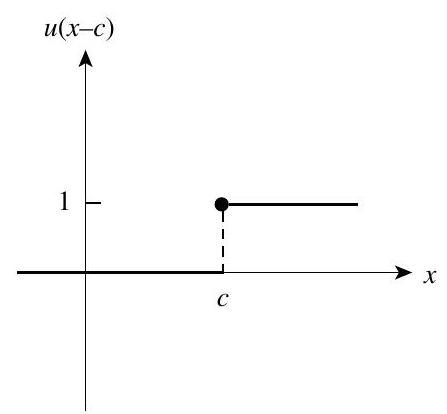
\includegraphics[max width=\textwidth]{2024_04_03_5bb5b4275a64cb9887d1g-252(2)}
\end{center}

Fig. 23-1

Theorem 23.3. $\mathscr{L}\{u(x-c)\}=\frac{1}{s} e^{-c s}$.

\section*{TRANSLATIONS}
Given a function $f(x)$ defined for $x \geq 0$, the function

$$
u(x-c) f(x-c)=\left\{\begin{array}{cc}
0 & x<c \\
f(x-c) & x \geq c
\end{array}\right.
$$

represents a shift, or translation, of the function $f(x)$ by $c$ units in the positive $x$-direction. For example, if $f(x)$ is given graphically by Fig. 23-2, then $u(x-c) f(x-c)$ is given graphically by Fig. 23-3.

\begin{center}
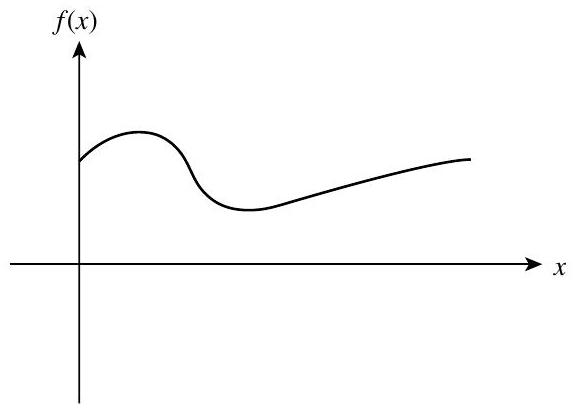
\includegraphics[max width=\textwidth]{2024_04_03_5bb5b4275a64cb9887d1g-252}
\end{center}

Fig. 23-2

\begin{center}
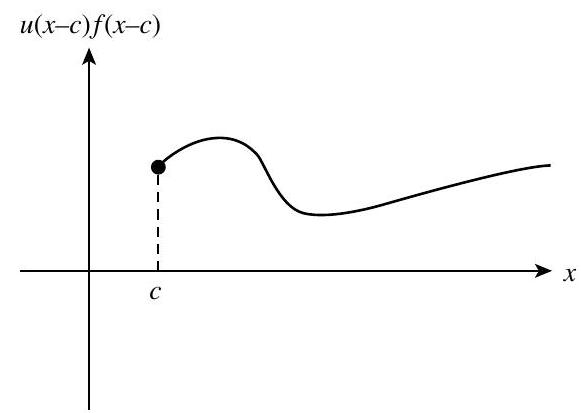
\includegraphics[max width=\textwidth]{2024_04_03_5bb5b4275a64cb9887d1g-252(1)}
\end{center}

Fig. 23-3

Theorem 23.4. If $F(s)=\mathscr{L}\{f(x)\}$, then

$$
\mathscr{L}\{u(x-c) f(x-c)\}=e^{-c s} F(s)
$$

Conversely,

$$
\mathscr{L}^{-1}\left\{e^{-c s} F(s)\right\}=u(x-c) f(x-c)=\left\{\begin{array}{cc}
0 & x<c \\
f(x-c) & x \geq c
\end{array}\right.
$$

\section*{Solved problems}
23.1. Find $f(x) * g(x)$ when $f(x)=e^{3 x}$ and $g(x)=e^{2 x}$.

Here $f(t)=e^{3 t}, g(x-t)=e^{2(x-t)}$, and

$$
\begin{aligned}
f(x) * g(x) & =\int_{0}^{x} e^{3 t} e^{2(x-t)} d t=\int_{0}^{x} e^{3 t} e^{2 x} e^{-2 t} d t \\
& =e^{2 x} \int_{0}^{x} e^{t} d t=e^{2 x}\left[e^{t}\right]_{t=0}^{t=x}=e^{2 x}\left(e^{x}-1\right)=e^{3 x}-e^{2 x}
\end{aligned}
$$

23.2. Find $g(x) * f(x)$ for the two functions in problem 23.1 and verify Theorem 23.1.

With $f(x-t)=e^{3(x-t)}$ and $g(t)=e^{2 t}$,

$$
\begin{aligned}
g(x) * f(x) & =\int_{0}^{x} g(t) f(x-t) d t=\int_{0}^{x} e^{2 t} e^{3(x-t)} d t \\
& =e^{3 x} \int_{0}^{x} e^{-t} d t=e^{3 x}\left[-e^{-t}\right]_{t=0}^{t=x} \\
& =e^{3 x}\left(-e^{-x}+1\right)=e^{3 x}-e^{2 x}
\end{aligned}
$$

which, from Problem 23.1 equals $f(x) * g(x)$.

23.3. Find $f(x) * g(x)$ when $f(x)=x$ and $g(x)=x^{2}$.

Here $f(t)=t$ and $g(x-t)=(x-t)^{2}=x^{2}-2 x t+t^{2}$. Thus,

$$
\begin{aligned}
f(x) * g(x) & =\int_{0}^{x} t\left(x^{2}-2 x t+t^{2}\right) d t \\
& =x^{2} \int_{0}^{x} t d t-2 x \int_{0}^{x} t^{2} d t+\int_{0}^{x} t^{3} d t \\
& =x^{2} \frac{x^{2}}{2}-2 x \frac{x^{3}}{3}+\frac{x^{4}}{4}=\frac{1}{12} x^{4}
\end{aligned}
$$

23.4. Find $\mathscr{L}^{-1}\left\{\frac{1}{s^{2}-5 s+6}\right\}$ by convolutions.

Note that

$$
\frac{1}{s^{2}-5 s+6}=\frac{1}{(s-3)(s-2)}=\frac{1}{s-3} \frac{1}{s-2}
$$

Defining $F(s)=1 /(s-3)$ and $G(s)=1 /(s-2)$, we have from Appendix A that $f(x)=e^{3 x}$ and $g(x)=e^{2 x}$. It follows from Eq. (23.2) and the results of Problem 23.1 that

$$
\mathscr{L}^{-1}\left\{\frac{1}{s^{2}-5 s+6}\right\}=f(x) * g(x)=e^{3 x} * e^{2 x}=e^{3 x}-e^{2 x}
$$

23.5. Find $\mathscr{L}^{-1}\left\{\frac{6}{s^{2}-1}\right\}$ by convolutions.

Note that

$$
\mathscr{L}^{-1}\left\{\frac{6}{s^{2}-1}\right\}=\mathscr{L}^{-1}\left\{\frac{6}{(s-1)(s+1)}\right\}=6 \mathscr{L}^{-1}\left\{\frac{1}{(s-1)} \frac{1}{(s+1)}\right\}
$$

Defining $F(s)=1 /(s-1)$ and $G(s)=1 /(s+1)$, we have from Appendix A that $f(x)=e^{x}$ and $g(x)=e^{-x}$. It follows from Eq. (23.2) that

$$
\begin{aligned}
\mathscr{L}^{-1}\left\{\frac{6}{s^{2}-1}\right\} & =6 \mathscr{L}^{-1}\{F(s) G(s)\}=6 e^{x} * e^{-x} \\
& =6 \int_{0}^{x} e^{t} e^{-(x-t)} d t=6 e^{-x} \int_{0}^{x} e^{2 t} d t \\
& =6 e^{-x}\left[\frac{e^{2 x}-1}{2}\right]=3 e^{x}-3 e^{-x}
\end{aligned}
$$

23.6. Find $\mathscr{L}^{-1}\left\{\frac{1}{s\left(s^{2}+4\right)}\right\}$ by convolutions.

Note that

$$
\frac{1}{s\left(s^{2}+4\right)}=\frac{1}{s} \frac{1}{s^{2}+4}
$$

Defining $F(s)=1 / s$ and $G(s)=1 /\left(s^{2}+4\right)$, we have from Appendix A that $f(x)=1$ and $g(x)=\frac{1}{2} \sin 2 x$. It now follows from Eq. (23.2) that

$$
\begin{aligned}
\mathscr{L}^{-1}\left\{\frac{1}{s\left(s^{2}+4\right)}\right\} & =\mathscr{L}^{-1}\{F(s) G(s)\}=g(x) * f(x) \\
& =\int_{0}^{x} g(t) f(x-t) d t=\int_{0}^{x}\left(\frac{1}{2} \sin 2 t\right)(1) d t \\
& =\frac{1}{4}(1-\cos 2 x)
\end{aligned}
$$

See also Problem 22.19.

23.7. Find $\mathscr{L}^{-1}\left\{\frac{1}{(s-1)^{2}}\right\}$ by convolutions.

If we define $F(s)=G(s)=1 /(s-1)$, then $f(x)=g(x)=e^{x}$ and

$$
\begin{aligned}
\mathscr{L}^{-1}\left\{\frac{1}{(s-1)^{2}}\right\} & =\mathscr{L}^{-1}\{F(s) G(s)\}=f(x) * g(x) \\
& =\int_{0}^{x} f(t) g(x-t) d t=\int_{0}^{x} e^{t} e^{x-t} d t \\
& =e^{x} \int_{0}^{x}(1) d t=x e^{x}
\end{aligned}
$$

23.8. Use the definition of the Laplace transform to find $\mathscr{L}\{u(x-c)\}$ and thereby prove Theorem 23.3.

It follows directly from Eq. (21.1) that

$$
\begin{aligned}
\mathscr{L}\{u(x-c)\} & =\int_{0}^{\infty} e^{-s x} u(x-c) d x=\int_{0}^{c} e^{-s x}(0) d x+\int_{c}^{\infty} e^{-s x}(1) d x \\
& =\int_{c}^{\infty} e^{-s x} d x=\lim _{R \rightarrow \infty} \int_{c}^{R} e^{-s x} d x=\lim _{R \rightarrow \infty} \frac{e^{-s R}-e^{-s c}}{-s} \\
& =\frac{1}{s} e^{-s c} \quad(\text { if } s>0)
\end{aligned}
$$

23.9. Graph the function $f(x)=u(x-2)-u(x-3)$.

Note that

Thus,

$$
\begin{aligned}
& u(x-2)=\left\{\begin{array}{ll}
0 & x<2 \\
1 & x \geq 2
\end{array} \text { and } u(x-3)= \begin{cases}0 & x<3 \\
1 & x \geq 3\end{cases} \right. \\
& f(x)=u(x-2)-u(x-3)=\left\{\begin{array}{lr}
0-0=0 & x<2 \\
1-0=1 & 2 \leq x<3 \\
1-1=0 & x \geq 3
\end{array}\right.
\end{aligned}
$$

the graph of which is given in Fig. 23-4.

23.10. Graph the function $f(x)=5-5 u(x-8)$ for $x \geq 0$.

Note that

$$
\begin{gathered}
5 u(x-8)= \begin{cases}0 & x<8 \\
5 & x \geq 8\end{cases} \\
f(x)=5-5 u(x-8)= \begin{cases}5 & x<8 \\
0 & x \geq 8\end{cases}
\end{gathered}
$$

Thus

The graph of this function when $x \geq 0$ is given in Fig. 23-5.

\begin{center}
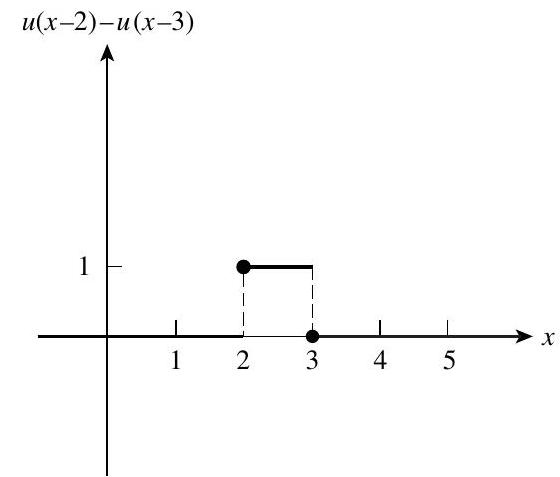
\includegraphics[max width=\textwidth]{2024_04_03_5bb5b4275a64cb9887d1g-255}
\end{center}

Fig. 23-4

\begin{center}
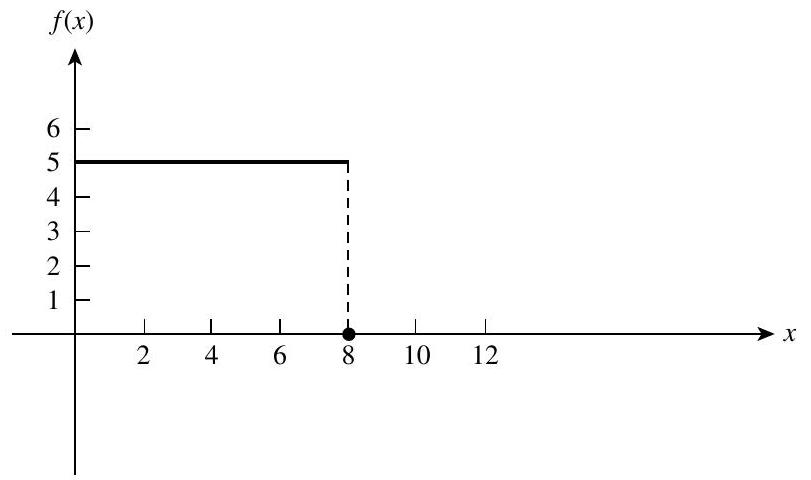
\includegraphics[max width=\textwidth]{2024_04_03_5bb5b4275a64cb9887d1g-255(1)}
\end{center}

Fig. 23-5

23.11. Use the unit step function to give an analytic representation of the function $f(x)$ graphed in Fig. 23-6.

Note that $f(x)$ is the function $g(x)=x, x \geq 0$, translated four units in the positive $x$-direction. Thus, $f(x)=u(x-4) g(x-4)=(x-4) u(x-4)$.

23.12. Use the unit step function to give an analytic description of the function $g(x)$ graphed on the interval $(0, \infty)$ in Fig. 23-7. If on the subinterval $(0, a)$ the graph is identical to Fig. 23-2.

Let $f(x)$ represent the function graphed in Fig. 23-2. Then $g(x)=f(x)[1-u(x-a)]$.

\begin{center}
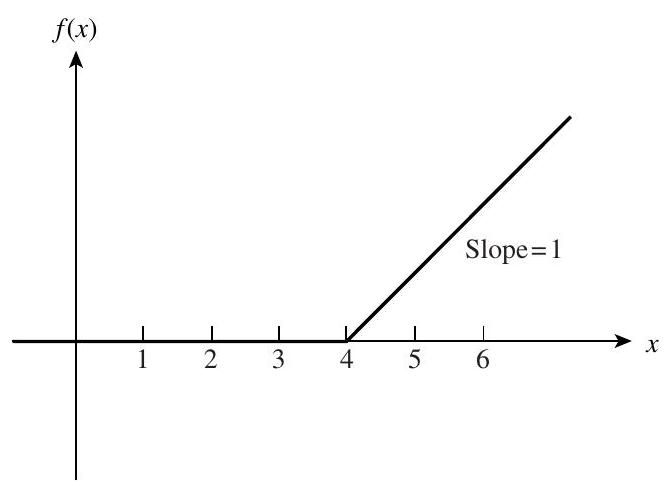
\includegraphics[max width=\textwidth]{2024_04_03_5bb5b4275a64cb9887d1g-256(1)}
\end{center}

Fig. 23-6

\begin{center}
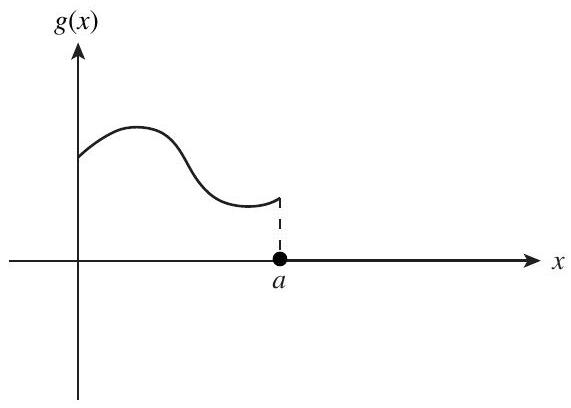
\includegraphics[max width=\textwidth]{2024_04_03_5bb5b4275a64cb9887d1g-256}
\end{center}

Fig. 23-7

23.13. Find $\mathscr{L}\{g(x)\}$ if $g(x)=\left\{\begin{array}{cc}0 & x<4 \\ (x-4)^{2} & x \geq 4\end{array}\right.$.

If we define $f(x)=x^{2}$, then $g(x)$ can be given compactly as $g(x)=u(x-4) f(x-4)=u(x-4)(x-4)^{2}$. Then, noting that $\mathscr{L}\{f(x)\}=F(s)=2 / s^{3}$ and using Theorem 23.4, we conclude that

$$
\mathscr{L}\{g(x)\}=\mathscr{L}\left\{u(x-4)(x-4)^{2}\right\}=e^{-4 s} \frac{2}{s^{3}}
$$

23.14. Find $\mathscr{L}\{g(x)\}$ if $g(x)=\left\{\begin{array}{cc}0 & x<4 \\ x^{2} & x \geq 4\end{array}\right.$.

We first determine a function $f(x)$ such that $f(x-4)=x^{2}$. Once this has been done, $g(x)$ can be written as $g(x)=u(x-4) f(x-4)$ and Theorem 23.4 can be applied. Now, $f(x-4)=x^{2}$ only if

$$
f(x)=f(x+4-4)=(x+4)^{2}=x^{2}+8 x+16
$$

Since

$$
\mathscr{L}\{f(x)\}=\mathscr{L}\left\{x^{2}\right\}+8 \mathscr{L}\{x\}+16 \mathscr{L}\{1\}=\frac{2}{s^{3}}+\frac{8}{s^{2}}+\frac{16}{s}
$$

it follows that

$$
\mathscr{L}\{g(x)\}=\mathscr{L}\{u(x-4) f(x-4)\}=e^{-4 s}\left(\frac{2}{s^{3}}+\frac{8}{s^{2}}+\frac{16}{s}\right)
$$

23.15. Prove Theorem 23.1.

Making the substitution $\tau=x-t$ in the right-hand side of Eq. (23.1), we have

$$
\begin{aligned}
f(x) * g(x) & =\int_{0}^{x} f(t) g(x-t) d t=\int_{x}^{0} f(x-\tau) g(\tau)(-d \tau) \\
& =-\int_{x}^{0} g(\tau) f(x-\tau) d \tau=\int_{0}^{x} g(\tau) f(x-\tau) d \tau \\
& =g(x) * f(x)
\end{aligned}
$$

23.16. Prove that $f(x) *[g(x)+h(x)]=f(x) * g(x)+f(x) * h(x)$.

$$
\begin{aligned}
f(x) *[g(x)+h(x)] & =\int_{0}^{x} f(t)[g(x-t)+h(x-t)] d t \\
& =\int_{0}^{x}[f(t) g(x-t)+f(t) h(x-t)] d t \\
& =\int_{0}^{x} f(t) g(x-t) d t+\int_{0}^{x} f(t) h(x-t) d t \\
& =f(x) * g(x)+f(x) * h(x)
\end{aligned}
$$

23.17. The following equation is called an integral equation of convolution type.

Assuming that the Laplace Transform for $y(x)$ exists, we solve this equation, and the next two examples, for $y(x)$.

$$
y(x)=x+\int_{0}^{x} y(t) \sin (x-t) d t
$$

We see that this integral equation can be written as $y(x)=x+y(x) * \sin x$. Taking the Laplace transform $\mathscr{L}$ of both sides and applying Theorem 23.2, we have

$$
\mathscr{L}\{y\}=\mathscr{L}\{x\}+\mathscr{L}\{y\} \mathscr{L}\{\sin x\}=\frac{1}{s^{2}}+\mathscr{L}\{y\} \frac{1}{s^{2}+1} .
$$

Solving for $\mathscr{L}\{y\}$ yields

$$
\mathscr{L}\{y\}=\frac{s^{2}+1}{s^{4}} .
$$

This implies that $y(x)=x+\frac{x^{3}}{6}$, which is indeed the solution, as can be verified by direct substitution as follows:

$$
x+\int_{0}^{x}\left(t+\frac{t^{3}}{6}\right) \sin (x-t) d t=x+\frac{x^{3}}{6}=y(x)
$$

23.18. Use Laplace Transforms to solve the integral equation of convolution type:

$$
y(x)=2-\int_{0}^{x} y(t) e^{x-t} d t
$$

Here we have $y(x)=2-y(x) * e^{x}$. Continuing as in Problem 23.17, we find that

$$
\mathscr{L}\{y\}=\frac{2 s-2}{s^{2}}
$$

which gives $y(x)=2-2 x$ as the desired solution.

23.19. Use Laplace Transforms to solve the integral equation of convolution type:

$$
y(x)=x^{3}+\int_{0}^{x} 4 y(t) d t
$$

the solution.

Noting that $y(x)=x^{3}+4 * y(x)$, we find that $\mathscr{L}\{y\}=\frac{6}{s^{3}(s-4)}$ which gives $y(x)=\frac{3}{32}\left(-1+e^{4 x}-4 x-8 x^{2}\right)$ as\\
solution.

\section*{Supplementary problems}
23.20. Find $x * x$.

23.22. Find $4 x * \mathrm{e}^{2 x}$.

23.24. Find $x * e^{x}$.

23.26. Find $3 * \sin 2 x$.\\
23.21. Find $2 * x$.

23.23. Find $e^{4 x} * e^{-2 x}$.

23.25. Find $x * x e^{-x}$.

23.27. Find $x * \cos x$.

In Problems 23.28 through 23.35, use convolutions to find the inverse Laplace transforms of the given functions.

23.28. $\frac{1}{(s-1)(s-2)}$

23.30. $\frac{2}{s(s+1)}$

23.32. $\frac{3}{s^{2}\left(s^{2}+3\right)}$

23.33. $\frac{1}{s\left(s^{2}+4\right)}$ with $F(s)=1 / s^{2}$ and $G(s)=s /\left(s^{2}+4\right)$. Compare with Problem 23.6.

23.34. $\frac{9}{s\left(s^{2}+9\right)}$

23.35. $\frac{9}{s^{2}\left(s^{2}+9\right)}$

23.36. Graph $f(x)=2 u(x-2)-u(x-4)$.

23.37. Graph $f(x)=u(x-2)-2 u(x-3)+u(x-4)$.

23.38. Use the unit step function to give an analytic representation for the function graphed in Fig. 23-8.

\begin{center}
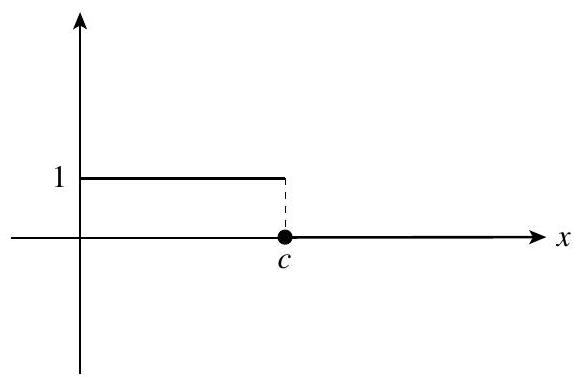
\includegraphics[max width=\textwidth]{2024_04_03_5bb5b4275a64cb9887d1g-258}
\end{center}

Fig. 23-8

23.39. Graph $f(x)=u(x-\pi) \cos 2(x-\pi)$.

23.40. Graph $f(x)=\frac{1}{2}(x-1)^{2} u(x-1)$.

In Problems 23.41 through 23.48, find $\mathscr{L}\{g(x)\}$ for the given functions.

23.41. $g(x)=\left\{\begin{array}{cc}0 & x<1 \\ \sin (x-1) & x \geq 1\end{array}\right.$

23.42. $g(x)=\left\{\begin{array}{cc}0 & x<3 \\ x-3 & x \geq 3\end{array}\right.$

23.43. $g(x)= \begin{cases}0 & x<3 \\ x & x \geq 3\end{cases}$

23.44. $g(x)=\left\{\begin{array}{cc}0 & x<3 \\ x+1 & x \geq 3\end{array}\right.$

23.45. $g(x)=\left\{\begin{array}{cc}0 & x<5 \\ e^{x-5} & x \geq 5\end{array}\right.$

23.46. $g(x)=\left\{\begin{array}{cc}0 & x<5 \\ e^{x} & x \geq 5\end{array}\right.$

23.47. $g(x)=\left\{\begin{array}{cc}0 & x<2 \\ e^{x-5} & x \geq 2\end{array}\right.$

23.48. $g(x)=\left\{\begin{array}{cc}0 & x<2 \\ x^{3}+1 & x \geq 2\end{array}\right.$

In Problems 23.49 through 23.55, determine the inverse Laplace transforms of the given functions.

23.49. $\frac{s}{s^{2}+4} e^{-3 s}$

23.51. $\frac{1}{s^{2}+4} e^{-\pi s}$

23.53. $\frac{8}{s+3} e^{-s}$

23.55. $\frac{1}{s^{2}} e^{-\pi s}$

23.56. Prove that for any constant $k,[k f(x)] * g(x)=k[f(x) * g(x)]$.

In Problems 23.57 through 23.60, assume that the Laplace Transform for $y(x)$ exists. Solve for $y(x)$.

23.57. $y(x)=x^{3}+\int_{0}^{x}(x-t) y(t) d t$

23.58. $y(x)=e^{x}+\int_{0}^{x} y(t) d t$

23.59. $y(x)=1+\int_{0}^{x}(t-x) y(t) d t$

23.60. $y(x)=\int_{0}^{x}(t-x) y(t) d t$\\
23.50. $\frac{1}{s^{2}+4} e^{-5 s}$

23.52. $\frac{2}{s-3} e^{-2 s}$

23.54. $\frac{1}{s^{3}} e^{-2 s}$

\section*{$\rightarrow$ \\
 Solutions of Linear Differential Equations with Constant Coefficients by Laplace Transforms}
\section*{LAPLACE TRANSFORMS OF DERIVATIVES}
Denote $\mathscr{L}\{y(x)\}$ by $Y(s)$. Then under broad conditions, the Laplace transform of the $n$ th-derivative $(n=1,2,3, \ldots)$ of $y(x)$ is


\begin{equation*}
\mathscr{L}\left\{\frac{d^{n} y}{d x^{n}}\right\}=s^{n} Y(s)-s^{n-1} y(0)-s^{n-2} y^{\prime}(0)-\cdots-s y^{(n-2)}(0)-y^{(n-1)}(0) \tag{24.1}
\end{equation*}


If the initial conditions on $y(x)$ at $x=0$ are given by


\begin{equation*}
y(0)=c_{0}, \quad y^{\prime}(0)=c_{1}, \ldots, y^{(n-1)}(0)=c_{n-1} \tag{24.2}
\end{equation*}


then (24.1) can be rewritten as


\begin{equation*}
\mathscr{L}\left\{\frac{d^{n} y}{d x^{n}}\right\}=s^{n} Y(s)-c_{0} s^{n-1}-c_{1} s^{n-2}-\cdots-c_{n-2} s-c_{n-1} \tag{24.3}
\end{equation*}


For the special cases of $n=1$ and $n=2$, Eq. (24.3) simplifies to


\begin{gather*}
\mathscr{L}\left\{y^{\prime}(x)\right\}=s Y(s)-c_{0}  \tag{24.4}\\
\mathscr{L}\left\{y^{\prime \prime}(x)\right\}=s^{2} Y(s)-c_{0} s-c_{1} \tag{24.5}
\end{gather*}


\section*{SOLUTIONS OF DIFFERENTIAL EQUATIONS}
Laplace transforms are used to solve initial-value problems given by the $n$ th-order linear differential equation with constant coefficients


\begin{equation*}
b_{n} \frac{d^{n} y}{d x^{n}}+b_{n-1} \frac{d^{n-1} y}{d x^{n-1}}+\cdots+b_{1} \frac{d y}{d x}+b_{0} y=g(x) \tag{24.6}
\end{equation*}


together with the initial conditions specified in Eq. (24.2). First, take the Laplace transform of both sides of Eq. (24.6), thereby obtaining an algebraic equation for $Y(s)$. Then solve for $Y(s)$ algebraically, and finally take inverse Laplace transforms to obtain $y(x)=\mathscr{L}^{-1}\{Y(s)\}$.

Unlike previous methods, where first the differential equation is solved and then the initial conditions are applied to evaluate the arbitrary constants, the Laplace transform method solves the entire initial-value problem in one step. There are two exceptions: when no initial conditions are specified and when the initial conditions are not at $x=0$. In these situations, $c_{0}$ through $c_{n}$ in Eqs. (24.2) and (24.3) remain arbitrary and the solution to differential Eq. (24.6) is found in terms of these constants. They are then evaluated separately when appropriate subsidiary conditions are provided. (See Problems 24.11 through 24.13.)

\section*{Solved problems}
24.1. Solve $y^{\prime}-5 y=0 ; y(0)=2$.

Taking the Laplace transform of both sides of this differential equation and using Property 24.4, we obtain $\mathscr{L}\left\{y^{\prime}\right\}-5 \mathscr{L}\{y\}=\mathscr{L}\{0\}$. Then, using Eq. (24.4) with $c_{0}=2$, we find

$$
[s Y(s)-2]-5 Y(s)=0 \text { from which } Y(s)=\frac{2}{s-5}
$$

Finally, taking the inverse Laplace transform of $Y(s)$, we obtain

$$
y(x)=\mathscr{L}^{-1}\{Y(s)\}=\mathscr{L}^{-1}\left\{\frac{2}{s-5}\right\}=2 \mathscr{L}^{-1}\left\{\frac{1}{s-5}\right\}=2 e^{5 x}
$$

24.2. Solve $y^{\prime}-5 y=e^{5 x} ; y(0)=0$.

Taking the Laplace transform of both sides of this differential equation and using Property 24.4, we find that $\mathscr{L}\left\{y^{\prime}\right\}-5 \mathscr{L}\{y\}=\mathscr{L}\left\{e^{5 x}\right\}$. Then, using Appendix A and Eq. (24.4) with $c_{0}=0$, we obtain

$$
[s Y(s)-0]-5 Y(s)=\frac{1}{s-5} \text { from which } \quad Y(s)=\frac{1}{(s-5)^{2}}
$$

Finally, taking the inverse transform of $Y(s)$, we obtain

$$
y(x)=\mathscr{L}^{-1}\{Y(s)\}=\mathscr{L}^{-1}\left\{\frac{1}{(s-5)^{2}}\right\}=x e^{5 x}
$$

(see Appendix A, entry 14).

24.3. Solve $y^{\prime}+y=\sin x ; y(0)=1$.

Taking the Laplace transform of both sides of the differential equation, we obtain

$$
\mathscr{L}\left\{y^{\prime}\right\}+\mathscr{L}\{y\}=\mathscr{L}\{\sin x\} \quad \text { or } \quad[s Y(s)-1]+Y(s)=\frac{1}{s^{2}+1}
$$

Solving for $Y(s)$, we find

$$
Y(s)=\frac{1}{(s+1)\left(s^{2}+1\right)}+\frac{1}{s+1}
$$

Taking the inverse Laplace transform, and using the result of Problem 22.17, we obtain

$$
\begin{aligned}
y(x) & =\mathscr{L}^{-1}\{Y(s)\}=\mathscr{L}^{-1}\left\{\frac{1}{(s+1)\left(s^{2}+1\right)}\right\}+\mathscr{L}^{-1}\left\{\frac{1}{s+1}\right\} \\
& =\left(\frac{1}{2} e^{-x}-\frac{1}{2} \cos x+\frac{1}{2} \sin x\right)+e^{-x}=\frac{3}{2} e^{-x}-\frac{1}{2} \cos x+\frac{1}{2} \sin x
\end{aligned}
$$

24.4. Solve $y^{\prime \prime}+4 y=0 ; y(0)=2, y^{\prime}(0)=2$.

Taking Laplace transforms, we have $\mathscr{L}\left\{y^{\prime \prime}\right\}+4 \mathscr{L}\{y\}=\mathscr{L}\{0\}$. Then, using Eq. (24.5) with $c_{0}=2$ and $c_{1}=2$, we obtain

or

$$
\begin{gathered}
{\left[s^{2} Y(s)-2 s-2\right]+4 Y(s)=0} \\
Y(s)=\frac{2 s+2}{s^{2}+4}=\frac{2 s}{s^{2}+4}+\frac{2}{s^{2}+4}
\end{gathered}
$$

Finally, taking the inverse Laplace transform, we obtain

$$
y(x)=\mathscr{L}^{-1}\{Y(s)\}=2 \mathscr{L}^{-1}\left\{\frac{s}{s^{2}+4}\right\}+\mathscr{L}^{-1}\left\{\frac{2}{s^{2}+4}\right\}=2 \cos 2 x+\sin 2 x
$$

24.5. Solve $y^{\prime \prime}-3 y^{\prime}+4 y=0 ; y(0)=1, y^{\prime}(0)=5$.

Taking Laplace transforms, we obtain $\mathscr{L}\left\{y^{\prime \prime}\right\}-3 \mathscr{L}\left\{y^{\prime}\right\}+4 \mathscr{L}\{y\}=\mathscr{L}\{0\}$. Then, using both Eqs. (24.4) and (24.5) with $c_{0}=1$ and $c_{1}=5$, we have

or

$$
\begin{gathered}
{\left[s^{2} Y(s)-s-5\right]-3[s Y(s)-1]+4 Y(s)=0} \\
Y(s)=\frac{s+2}{s^{2}-3 s+4}
\end{gathered}
$$

Finally, taking the inverse Laplace transform and using the result of Problem 22.10, we obtain

$$
y(x)=e^{(3 / 2) x} \cos \frac{\sqrt{7}}{2} x+\sqrt{7} e^{(3 / 2) x} \sin \frac{\sqrt{7}}{2} x
$$

24.6. Solve $y^{\prime \prime}-y^{\prime}-2 y=4 x^{2} ; y(0)=1, y^{\prime}(0)=4$.

Taking Laplace transforms, we have $\mathscr{L}\left\{y^{\prime \prime}\right\}-\mathscr{L}\left\{y^{\prime}\right\}-2 \mathscr{L}\{y\}=4 \mathscr{L}\left\{x^{2}\right\}$. Then, using both Eqs. (24.4) and (24.5) with $c_{0}=1$ and $c_{1}=4$, we obtain

$$
\left[s^{2} Y(s)-s-4\right]-[s Y(s)-1]-2 Y(s)=\frac{8}{s^{3}}
$$

or, upon solving for $Y(s)$,

$$
Y(s)=\frac{s+3}{s^{2}-s-2}+\frac{8}{s^{3}\left(s^{2}-s-2\right)}
$$

Finally, taking the inverse Laplace transform and using the results of Problems 22.15 and 22.16, we obtain

$$
\begin{aligned}
y(x) & =\left(\frac{5}{3} e^{2 x}-\frac{2}{3} e^{-x}\right)+\left(-3+2 x-2 x^{2}+\frac{1}{3} e^{2 x}+\frac{8}{3} e^{-x}\right) \\
& =2 e^{2 x}+2 e^{-x}-2 x^{2}+2 x-3
\end{aligned}
$$

(See Problem 13.1.)

24.7. Solve $y^{\prime \prime}+4 y^{\prime}+8 y=\sin x ; y(0)=1, y^{\prime}(0)=0$.

Taking Laplace transforms, we obtain $\mathscr{L}\left\{y^{\prime \prime}\right\}+4 \mathscr{L}\left\{y^{\prime}\right\}+8 \mathscr{L}\{y\}=\mathscr{L}\{\sin x\}$. Since $c_{0}=1$ and $c_{1}=0$, this becomes

Thus,

$$
\begin{gathered}
{\left[s^{2} Y(s)-s-0\right]+4[s Y(s)-1]+8 Y(s)=\frac{1}{s^{2}+1}} \\
Y(s)=\frac{s+4}{s^{2}+4 s+8}+\frac{1}{\left(s^{2}+1\right)\left(s^{2}+4 s+8\right)}
\end{gathered}
$$

Finally, taking the inverse Laplace transform and using the results of Problems 22.9 and 22.18, we obtain

$$
\begin{aligned}
y(x)= & \left(e^{-2 x} \cos 2 x+e^{-2 x} \sin 2 x\right) \\
& +\left(-\frac{4}{65} \cos x+\frac{7}{65} \sin x+\frac{4}{65} e^{-2 x} \cos 2 x+\frac{1}{130} e^{-2 x} \sin 2 x\right) \\
= & e^{-2 x}\left(\frac{69}{65} \cos 2 x+\frac{131}{130} \sin 2 x\right)+\frac{7}{65} \sin x-\frac{4}{65} \cos x
\end{aligned}
$$

(See Problem 13.3.)

24.8. Solve $y^{\prime \prime}-2 y^{\prime}+y=f(x) ; y(0)=0, y^{\prime}(0)=0$.

In this equation $f(x)$ is unspecified. Taking Laplace transforms and designating $\mathscr{L}\{f(x)\}$ by $F(s)$, we obtain

$$
\left[s^{2} Y(s)-(0) s-0\right]-2[s Y(s)-0]+Y(s)=F(s) \quad \text { or } \quad Y(s)=\frac{F(s)}{(s-1)^{2}}
$$

From Appendix A, entry 14, $\mathscr{L}^{-1}\left\{1 /(s-1)^{2}\right\}=x e^{x}$. Thus, taking the inverse transform of $Y(s)$ and using convolutions, we conclude that

$$
y(x)=x e^{x} * f(x)=\int_{0}^{x} t e^{t} f(x-t) d t
$$

24.9. Solve $y^{\prime \prime}+y=f(x) ; y(0)=0, y^{\prime}(0)=0$ if $f(x)= \begin{cases}0 & x<1 \\ 2 & x \geq 1\end{cases}$

Note that $f(x)=2 u(x-1)$. Taking Laplace transforms, we obtain

$$
\left[s^{2} Y(s)-(0) s-0\right]+Y(s)=\mathscr{L}\{f(x)\}=2 \mathscr{L}\{u(x-1)\}=2 e^{-s} / s
$$

or

$$
Y(s)=e^{-s} \frac{2}{s\left(s^{2}+1\right)}
$$

Since

$$
\mathscr{L}^{-1}\left\{\frac{2}{s\left(s^{2}+1\right)}\right\}=2 \mathscr{L}^{-1}\left\{\frac{1}{s}\right\}-2 \mathscr{L}^{-1}\left\{\frac{s}{s^{2}+1}\right\}=2-2 \cos x
$$

it follows from Theorem 23.4 that

$$
y(x)=\mathscr{L}^{-1}\left\{e^{-s} \frac{2}{s\left(s^{2}+1\right)}\right\}=[2-2 \cos (x-1)] u(x-1)
$$

24.10. Solve $y^{\prime \prime \prime}+y^{\prime}=e^{x} ; y(0)=y^{\prime}(0)=y^{\prime \prime}(0)=0$. we have

Taking Laplace transforms, we obtain $\mathscr{L}\left\{y^{\prime \prime \prime}\right\}+\mathscr{L}\left\{y^{\prime}\right\}=\mathscr{L}\left(e^{x}\right)$. Then, using Eq. (24.3) with $n=3$ and Eq. (24.4),

$$
\left[s^{3} Y(s)-(0) s^{2}-(0) s-0\right]+[s Y(s)-0]=\frac{1}{s-1} \quad \text { or } \quad Y(s)=\frac{1}{(s-1)\left(s^{3}+s\right)}
$$

Finally, using the method of partial fractions and taking the inverse transform, we obtain

$$
y(x)=\mathscr{L}^{-1}\left\{-\frac{1}{s}+\frac{\frac{1}{2}}{s-1}+\frac{\frac{1}{2} s-\frac{1}{2}}{s^{2}+1}\right\}=-1+\frac{1}{2} e^{x}+\frac{1}{2} \cos x-\frac{1}{2} \sin x
$$

24.11. Solve $y^{\prime}-5 y=0$.

No initial conditions are specified. Taking the Laplace transform of both sides of the differential equation, we obtain

$$
\mathscr{L}\left\{y^{\prime}\right\}-5 \mathscr{L}\{y\}=\mathscr{L}\{0\}
$$

Then, using Eq. (24.4) with $c_{0}=y(0)$ kept arbitrary, we have

$$
\left[s Y(s)-c_{0}\right]-5 Y(s)=0 \quad \text { or } \quad Y(s)=\frac{c_{0}}{s-5}
$$

Taking the inverse Laplace transform, we find that

$$
y(x)=\mathscr{L}^{-1}\{Y(s)\}=c_{0} \mathscr{L}^{-1}\left\{\frac{1}{s-5}\right\}=c_{0} e^{5 x}
$$

24.12. Solve $y^{\prime \prime}-3 y^{\prime}+2 y=e^{-x}$.

No initial conditions are specified. Taking Laplace transforms, we have $\mathscr{L}\left\{y^{\prime \prime}\right\}-3 \mathscr{L}\left\{y^{\prime}\right\}+2 \mathscr{L}\{y\}=\mathscr{L}\left(e^{-x}\right)$, or

$$
\left[s^{2} Y(s)-s c_{0}-c_{1}\right]-3\left[s Y(s)-c_{0}\right]+2[Y(s)]=1 /(s+1)
$$

Here $c_{0}$ and $c_{1}$ must remain arbitrary, since they represent $y(0)$ and $y^{\prime}(0)$, respectively, which are unknown. Thus,

$$
Y(s)=c_{0} \frac{s-3}{s^{2}-3 s+2}+c_{1} \frac{1}{s^{2}-3 s+2}+\frac{1}{(s+1)\left(s^{2}-3 s+2\right)}
$$

Using the method of partial fractions and noting that $s^{2}-3 s+2=(s-1)(s-2)$, we obtain

$$
\begin{aligned}
y(x) & =c_{0} \mathscr{L}^{-1}\left\{\frac{2}{s-1}+\frac{-1}{s-2}\right\}+c_{1} \mathscr{L}^{-1}\left\{\frac{-1}{s-1}+\frac{1}{s-2}\right\}+\mathscr{L}^{-1}\left\{\frac{1 / 6}{s+1}+\frac{-1 / 2}{s-1}+\frac{1 / 3}{s-2}\right\} \\
& =c_{0}\left(2 e^{x}-e^{2 x}\right)+c_{1}\left(-e^{x}+e^{2 x}\right)+\left(\frac{1}{6} e^{-x}-\frac{1}{2} e^{x}+\frac{1}{3} e^{2 x}\right) \\
& =\left(2 c_{0}-c_{1}-\frac{1}{2}\right) e^{x}+\left(-c_{0}+c_{1}+\frac{1}{3}\right) e^{2 x}+\frac{1}{6} e^{-x} \\
& =d_{0} e^{x}+d_{1} e^{2 x}+\frac{1}{6} e^{-x}
\end{aligned}
$$

where $d_{0}=2 c_{0}-c_{1}-\frac{1}{2}$ and $d_{1}=-c_{0}+c_{1}+\frac{1}{3}$.

24.13. Solve $y^{\prime \prime}-3 y^{\prime}+2 y=e^{-x} ; y(1)=0, y^{\prime}(1)=0$.

The initial conditions are given at $x=1$, not $x=0$. Using the results of Problem 24.12, we have as the solution to just the differential equation

$$
y=d_{0} e^{x}+d_{1} e^{2 x}+\frac{1}{6} e^{-x}
$$

Applying the initial conditions to this last equation, we find that $d_{0}=-\frac{1}{2} e^{-2}$ and $d_{1}=\frac{1}{3} e^{-3}$; hence,

$$
y(x)=-\frac{1}{2} e^{x-2}+\frac{1}{3} e^{2 x-3}+\frac{1}{6} e^{-x}
$$

24.14. Solve $\frac{d N}{d t}=0.05 N ; N(0)=20,000$.

This is a differential equation for the unknown function $N(t)$ in the independent variable $t$. We set $N(s)=\mathscr{L}\{N(t)\}$. Taking Laplace transforms of the given differential equation and using (24.4) with $N$ replacing $y$, we have

$$
\begin{aligned}
{[s N(s)-N(0)] } & =0.05 N(s) \\
{[s N(s)-20,000] } & =0.05 N(s)
\end{aligned}
$$

or, upon solving for $N(s)$,

$$
N(s)=\frac{20,000}{s-0.05}
$$

Then from Appendix A, entry 7 with $a=0.05$ and $t$ replacing $x$, we obtain

$$
N(t)=\mathscr{L}^{-1}\{N(s)\}=\mathscr{L}^{-1}\left\{\frac{20,000}{s-0.05}\right\}=20,000 \mathscr{L}^{-1}\left\{\frac{1}{s-0.05}\right\}=20,000 e^{0.05 t}
$$

Compare with (2) of Problem 7.1.

24.15. Solve $\frac{d I}{d t}+50 I=5 ; I(0)=0$.

This is a differential equation for the unknown function $I(t)$ in the independent variable $t$. We set $I(s)=\mathscr{L}\{I(t)\}$. Taking Laplace transforms of the given differential equation and using Eq. (24.4) with $I$ replacing $y$, we have

$$
\begin{aligned}
& {[s I(s)-I(0)]+50 I(s)=5\left(\frac{1}{s}\right)} \\
& {[s I(s)-0]+50 I(s)=5\left(\frac{1}{s}\right)}
\end{aligned}
$$

or, upon solving for $I(s)$,

$$
I(s)=\frac{5}{s(s+50)}
$$

Then using the method of partial fractions and Appendix A, with $t$ replacing $x$, we obtain

$$
\begin{aligned}
I(t) & =\mathscr{L}^{-1}\{I(s)\}=\mathscr{L}^{-1}\left\{\frac{5}{s(s+50)}\right\}=\mathscr{L}^{-1}\left\{\frac{1 / 10}{s}-\frac{1 / 10}{s+50}\right\} \\
& =\frac{1}{10} \mathscr{L}^{-1}\left\{\frac{1}{s}\right\}-\frac{1}{10} \mathscr{L}^{-1}\left\{\frac{1}{s+50}\right\}=\frac{1}{10}-\frac{1}{10} e^{-50 t}
\end{aligned}
$$

Compare with (1) of Problem 7.19.

24.16. Solve $\ddot{x}+16 x=2 \sin 4 t ; x(0)=-\frac{1}{2}, \dot{x}(0)=0$.

This is a differential equation for the unknown function $x(t)$ in the independent variable $t$. We set $X(s)=\mathscr{L}\{x(t)\}$. Taking Laplace transforms of the given differential equation and using Eq. (24.5) with $x$ replacing $y$, we have

$$
\begin{aligned}
{\left[s^{2} X(s)-s x(0)-\dot{x}(0)\right]+16 X(s) } & =2\left(\frac{4}{s^{2}+16}\right) \\
{\left[s^{2} X(s)-s\left(-\frac{1}{2}\right)-0\right]+16 X(s) } & =\frac{8}{s^{2}+16} \\
\left(s^{2}+16\right) X(s) & =\frac{8}{s^{2}+16}-\frac{s}{2}
\end{aligned}
$$

or

$$
X(s)=\frac{8}{\left(s^{2}+16\right)^{2}}-\frac{1}{2}\left(\frac{s}{s^{2}+16}\right)
$$

Then using Appendix A, entries 17 and 9 with $a=4$ and $t$ replacing $x$, we obtain

$$
\begin{aligned}
x(t)=\mathscr{L}^{-1}\{X(s)\} & =\mathscr{L}^{-1}\left\{\frac{8}{\left(s^{2}+16\right)^{2}}-\frac{1}{2}\left(\frac{s}{s^{2}+16}\right)\right\} \\
& =\frac{1}{16} \mathscr{L}^{-1}\left\{\frac{128}{\left(s^{2}+16\right)^{2}}\right\}-\frac{1}{2} \mathscr{L}^{-1}\left\{\frac{s}{s^{2}+16}\right\} \\
& =\frac{1}{16}(\sin 4 t-4 t \cos 4 t)-\frac{1}{2} \cos 4 t
\end{aligned}
$$

Compare with the results of Problem 14.10.

\section*{Supplementary Problems}
Use Laplace transforms to solve the following problems.\\
24.17. $y^{\prime}+2 y=0 ; y(0)=1$\\
24.18. $y^{\prime}+2 y=2 ; y(0)=1$\\
24.19. $y^{\prime}+2 y=e^{x} ; y(0)=1$\\
24.20. $y^{\prime}+2 y=0 ; y(1)=1$\\
24.21. $y^{\prime}+5 y=0 ; y(1)=0$\\
24.22. $y^{\prime}-5 y=e^{5 x} ; y(0)=2$\\
24.23. $y^{\prime}+y=x e^{-x} ; y(0)=-2$\\
24.24. $y^{\prime}+y=\sin x$\\
24.25. $y^{\prime}+20 y=6 \sin 2 x ; y(0)=6$\\
24.26. $y^{\prime \prime}-y=0 ; y(0)=1, y^{\prime}(0)=1$\\
24.27. $y^{\prime \prime}-y=\sin x ; y(0)=0, y^{\prime}(0)=1$\\
24.28. $y^{\prime \prime}-y=e^{x} ; y(0)=1, y^{\prime}(0)=0$\\
24.29. $y^{\prime \prime}+2 y^{\prime}-3 y=\sin 2 x ; y(0)=y^{\prime}(0)=0$\\
24.30. $y^{\prime \prime}+y=\sin x ; y(0)=0, y^{\prime}(0)=2$\\
24.31. $y^{\prime \prime}+y^{\prime}+y=0 ; y(0)=4, y^{\prime}(0)=-3$\\
24.32. $y^{\prime \prime}+2 y^{\prime}+5 y=3 e^{-2 x} ; y(0)=1, y^{\prime}(0)=1$\\
24.33. $y^{\prime \prime}+5 y^{\prime}-3 y=u(x-4) ; y(0)=0, y^{\prime}(0)=0$\\
24.34. $y^{\prime \prime}+y=0 ; y(\pi)=0, y^{\prime}(\pi)=-1$\\
24.35. $y^{\prime \prime \prime}-y=5 ; y(0)=0, y^{\prime}(0)=0, y^{\prime \prime}(0)=0$\\
24.36. $y^{(4)}-y=0 ; y(0)=1, y^{\prime}(0)=0, y^{\prime \prime}(0)=0, y^{\prime \prime \prime}(0)=0$\\
24.37. $\frac{d^{3} y}{d x^{3}}-3 \frac{d^{2} y}{d x^{2}}+3 \frac{d y}{d x}-y=x^{2} e^{x} ; y(0)=1, y^{\prime}(0)=2, y^{\prime \prime}(0)=3$\\
24.38. $\frac{d N}{d t}-0.085 N=0 ; N(0)=5000$\\
24.39. $\frac{d T}{d t}=3 T ; T(0)=100$\\
24.40. $\frac{d T}{d t}+3 T=90 ; T(0)=100$\\
24.41. $\frac{d v}{d t}+2 v=32$\\
24.42. $\frac{d q}{d t}+q=4 \cos 2 t ; q(0)=0$\\
24.43. $\ddot{x}+9 \dot{x}+14 x=0 ; x(0)=0, \dot{x}(0)=-1$\\
24.44. $\ddot{x}+4 \dot{x}+4 x=0 ; x(0)=2, \dot{x}(0)=-2$\\
24.45. $\frac{d^{2} x}{d t^{2}}+8 \frac{d x}{d t}+25 x=0 ; x(\pi)=0, \dot{x}(\pi)=6$\\
24.46. $\frac{d^{2} q}{d t^{2}}+9 \frac{d q}{d t}+14 q=\frac{1}{2} \sin t ; q(0)=0, \dot{q}(0)=1$

\section*{Solutions of Linear Systems by Laplace Transforms}
\section*{THE METHOD}
Laplace transforms are useful for solving systems of linear differential equations; that is, sets of two or more differential equations with an equal number of unknown functions. If all of the coefficients are constants, then the method of solution is a straightforward generalization of the one given in Chapter 24. Laplace transforms are taken of each differential equation in the system; the transforms of the unknown functions are determined algebraically from the resulting set of simultaneous equations; inverse transforms for the unknown functions are calculated with the help of Appendix A.

\section*{Solved Problems}
25.1. Solve the following system for the unknown functions $u(x)$ and $v(x)$ :

$$
\begin{aligned}
& u^{\prime}+u-v=0 \\
& v^{\prime}-u+v=2 \\
& u(0)=1, \quad v(0)=2
\end{aligned}
$$

Denote $\mathscr{L}\{u(x)\}$ and $\mathscr{L}\{v(x)\}$ by $U(s)$ and $V(s)$, respectively. Taking Laplace transforms of both differential equations, we obtain

$$
\begin{gathered}
{[s U(s)-1]+U(s)-V(s)=0} \\
{[s V(s)-2]-U(s)+V(s)=\frac{2}{s}} \\
(s+1) U(s)-V(s)=1 \\
-U(s)+(s+1) V(s)=\frac{2(s+1)}{s}
\end{gathered}
$$

The solution to this last set of simultaneous linear equations is

$$
U(s)=\frac{s+1}{s^{2}} \quad V(s)=\frac{2 s+1}{s^{2}}
$$

Taking inverse transforms, we obtain

$$
\begin{aligned}
& u(x)=\mathscr{L}^{-1}\{U(s)\}=\mathscr{L}^{-1}\left\{\frac{s+1}{s^{2}}\right\}=\mathscr{L}^{-1}\left\{\frac{1}{s}+\frac{1}{s^{2}}\right\}=1+x \\
& v(x)=\mathscr{L}^{-1}\{V(s)\}=\mathscr{L}^{-1}\left\{\frac{2 s+1}{s^{2}}\right\}=\mathscr{L}^{-1}\left\{\frac{2}{s}+\frac{1}{s^{2}}\right\}=2+x
\end{aligned}
$$

25.2. Solve the system

$$
\begin{aligned}
& y^{\prime}+z=x \\
& z^{\prime}+4 y=0 \\
& y(0)=1, \quad z(0)=-1
\end{aligned}
$$

Denote $\mathscr{L}\{y(x)\}$ and $\mathscr{L}\{z(x)\}$ by $Y(s)$ and $Z(s)$, respectively. Then, taking Laplace transforms of both differential equations, we obtain

$$
\begin{array}{lll}
{[s Y(s)-1]+Z(s)=\frac{1}{s^{2}}} & & s Y(s)+Z(s)=\frac{s^{2}+1}{s^{2}} \\
{[s Z(s)+1]+4 Y(s)=0} & \text { or } & 4 Y(s)+s Z(s)=-1
\end{array}
$$

The solution to this last set of simultaneous linear equations is

$$
Y(s)=\frac{s^{2}+s+1}{s\left(s^{2}-4\right)} \quad Z(s)=-\frac{s^{3}+4 s^{2}+4}{s^{2}\left(s^{2}-4\right)}
$$

Finally, using the method of partial fractions and taking inverse transforms, we obtain

$$
\begin{aligned}
y(x) & =\mathscr{L}^{-1}\{Y(s)\}=\mathscr{L}^{-1}\left\{-\frac{1 / 4}{s}+\frac{7 / 8}{s-2}+\frac{3 / 8}{s+2}\right\} \\
& =-\frac{1}{4}+\frac{7}{8} e^{2 x}+\frac{3}{8} e^{-2 x} \\
z(x) & =\mathscr{L}^{-1}\{Z(s)\}=\mathscr{L}^{-1}\left\{\frac{1}{s^{2}}-\frac{7 / 4}{s-2}+\frac{3 / 4}{s+2}\right\} \\
& =x-\frac{7}{4} e^{2 x}+\frac{3}{4} e^{-2 x}
\end{aligned}
$$

25.3. Solve the system

$$
\begin{aligned}
& w^{\prime}+y=\sin x \\
& y^{\prime}-z=e^{x} \\
& z^{\prime}+w+y=1 \\
& w(0)=0, \quad y(0)=1, \quad z(0)=1
\end{aligned}
$$

Denote $\mathscr{L}\{w(x)\}, \mathscr{L}\{y(x)\}$, and $\mathscr{L}\{z(x)\}$ by $W(s), Y(s)$, and $Z(s)$, respectively. Then, taking Laplace transforms\\
of all three differential equations, we have

$$
\begin{array}{rll}
{[s W(s)-0]+Y(s)=\frac{1}{s^{2}+1}} & & s W(s)+Y(s)=\frac{1}{s^{2}+1} \\
{[s Y(s)-1]-Z(s)=\frac{1}{s-1}} & \text { or } & s Y(s)-Z(s)=\frac{s}{s-1} \\
{[s Z(s)-1]+W(s)+Y(s)=\frac{1}{s}} & W(s)+Y(s)+s Z(s)=\frac{s+1}{s}
\end{array}
$$

The solution to this last system of simultaneous linear equations is

$$
W(s)=\frac{-1}{s(s-1)} \quad Y(s)=\frac{s^{2}+s}{(s-1)\left(s^{2}+1\right)} \quad Z(s)=\frac{s}{s^{2}+1}
$$

Using the method of partial fractions and then taking inverse transforms, we obtain

$$
\begin{aligned}
& w(x)=\mathscr{L}^{-1}\{W(s)\}=\mathscr{L}^{-1}\left\{\frac{1}{s}-\frac{1}{s-1}\right\}=1-e^{x} \\
& y(x)=\mathscr{L}^{-1}\{Y(s)\}=\mathscr{L}^{-1}\left\{\frac{1}{s-1}+\frac{1}{s^{2}+1}\right\}=e^{x}+\sin x \\
& z(x)=\mathscr{L}^{-1}\{Z(s)\}=\mathscr{L}^{-1}\left\{\frac{s}{s^{2}+1}\right\}=\cos x
\end{aligned}
$$

25.4. Solve the system

$$
\begin{aligned}
& y^{\prime \prime}+z+y=0 \\
& z^{\prime}+y^{\prime}=0 \\
& y(0)=0, \quad y^{\prime}(0)=0, \quad z(0)=1
\end{aligned}
$$

Taking Laplace transforms of both differential equations, we obtain

$$
\begin{array}{ccc}
{\left[s^{2} Y(s)-(0) s-(0)\right]+Z(s)+Y(s)=0} & \left(s^{2}+1\right) Y(s)+Z(s)=0 \\
{[s Z(s)-1]+[s Y(s)-0]=0} & \text { or } & Y(s)+Z(s)=\frac{1}{s}
\end{array}
$$

Solving this last system for $Y(s)$ and $Z(s)$, we find that

$$
Y(s)=-\frac{1}{s^{3}} \quad Z(s)=\frac{1}{s}+\frac{1}{s^{3}}
$$

Thus, taking inverse transforms, we conclude that

$$
y(x)=-\frac{1}{2} x^{2} \quad z(x)=1+\frac{1}{2} x^{2}
$$

25.5. Solve the system

$$
\begin{aligned}
& z^{\prime \prime}+y^{\prime}=\cos x \\
& y^{\prime \prime}-z=\sin x \\
& z(0)=-1, \quad z^{\prime}(0)=-1, \quad y(0)=1, \quad y^{\prime}(0)=0
\end{aligned}
$$

Taking Laplace transforms of both differential equations, we obtain

$$
\begin{array}{lll}
{\left[s^{2} Z(s)+s+1\right]+[s Y(s)-1]=\frac{s}{s^{2}+1}} & & s^{2} Z(s)+s Y(s)=-\frac{s^{3}}{s^{2}+1} \\
{\left[s^{2} Y(s)-s-0\right]-Z(s)=\frac{1}{s^{2}+1}} & \text { or } & -Z(s)+s^{2} Y(s)=\frac{s^{3}+s+1}{s^{2}+1}
\end{array}
$$

Solving this last system for $Z(s)$ and $Y(s)$, we find that

$$
Z(s)=-\frac{s+1}{s^{2}+1} \quad Y(s)=\frac{s}{s^{2}+1}
$$

Finally, taking inverse transforms, we obtain

$$
z(x)=-\cos x-\sin x \quad y(x)=\cos x
$$

25.6. Solve the system

$$
\begin{gathered}
w^{\prime \prime}-y+2 z=3 e^{-x} \\
-2 w^{\prime}+2 y^{\prime}+z=0 \\
2 w^{\prime}-2 y+z^{\prime}+2 z^{\prime \prime}=0 \\
w(0)=1, \quad w^{\prime}(0)=1, \quad y(0)=2, \quad z(0)=2, \quad z^{\prime}(0)=-2
\end{gathered}
$$

Taking Laplace transforms of all three differential equations, we find that

or

$$
\begin{gathered}
{\left[s^{2} W(s)-s-1\right]-Y(s)+2 Z(s)=\frac{3}{s+1}} \\
-2[s W(s)-1]+2[s Y(s)-2]+Z(s)=0 \\
2[s W(s)-1]-2 Y(s)+[s Z(s)-2]+2\left[s^{2} Z(s)-2 s+2\right]=0 \\
s^{2} W(s)-Y(s)+2 Z(s)=\frac{s^{2}+2 s+4}{s+1} \\
-2 s W(s)+2 s Y(s)+Z(s)=2 \\
2 s W(s)-2 Y(s)+\left(2 s^{2}+s\right) Z(s)=4 s
\end{gathered}
$$

The solution to this system is

$$
W(s)=\frac{1}{s-1} \quad Y(s)=\frac{2 s}{(s-1)(s+1)} \quad Z(s)=\frac{2}{s+1}
$$

Hence,

$$
w(x)=e^{x} \quad y(x)=\mathscr{L}^{-1}\left\{\frac{1}{s-1}+\frac{1}{s+1}\right\}=e^{x}+e^{-x} \quad z(x)=2 e^{-x}
$$

\section*{Supplementary Problems}
Use Laplace transforms to solve the following systems. All unknowns are functions of $x$.\\
25.7. $u^{\prime}-2 v=3$\\
25.8. $u^{\prime}+4 u-6 v=0$\\
$v^{\prime}+v-u=-x^{2}$\\
$v^{\prime}+3 u-5 v=0$\\
$u(0)=0, v(0)=-1$\\
$u(0)=3, v(0)=2$\\
25.9. $u^{\prime}+5 u-12 v=0$\\
25.10. $y^{\prime}+z=x$\\
$v^{\prime}+2 u-5 v=0$\\
$z^{\prime}-y=0 ;$\\
$u(0)=8, v(0)=3$\\
$y(0)=1, z(0)=0$

25.11. $y^{\prime}-z=0$

$y-z^{\prime}=0$

$y(0)=1, z(0)=1$

25.13. $w^{\prime}-y=0$

$w+y^{\prime}+z=1$

$w-y+z^{\prime}=2 \sin x$

$w(0)=1, y(0)=1, z(0)=1$

25.15. $u^{\prime \prime}-2 v=2$

$u+v^{\prime}=5 e^{2 x}+1$

$u(0)=2, u^{\prime}(0)=2, v(0)=1$

25.17. $w^{\prime \prime}+y+z=-1$

$w+y^{\prime \prime}-z=0$

$-w^{\prime}-y^{\prime}+z^{\prime \prime}=0$;

$w(0)=0, w^{\prime}(0)=1, y(0)=0$,

$y^{\prime}(0)=0, z(0)=-1, z^{\prime}(0)=1$\\
25.12. $w^{\prime}-w-2 y=1$

$y^{\prime}-4 w-3 y=-1 ;$

$w(0)=1, y(0)=2$

25.14. $u^{\prime \prime}+v=0$

$u^{\prime \prime}-v^{\prime}=-2 e^{x}$

$u(0)=0, u^{\prime}(0)=-2, v(0)=0, v^{\prime}(0)=2$

25.16. $w^{\prime \prime}-2 z=0$

$w^{\prime}+y^{\prime}-z=2 x$

$w^{\prime}-2 y+z^{\prime \prime}=0$

$w(0)=0, w^{\prime}(0)=0, y(0)=0$,

$z(0)=1, z^{\prime}(0)=0$

Solutions of Linear\\
Differential Equations\\
with Constant\\
Coefficients by Matrix\\
Methods

\section*{SOLUTION OF THE INITIAL-VALUE PROBLEM}
By the procedure of Chapter 17, any initial-value problem in which the differential equations are all linear with constant coefficients, can be reduced to the matrix system


\begin{equation*}
\dot{\mathbf{x}}(t)=\mathbf{A x}(t)+\mathbf{f}(t) ; \quad \mathbf{x}\left(t_{0}\right)=\mathbf{c} \tag{26.1}
\end{equation*}


where $\mathbf{A}$ is a matrix of constants. The solution to Eq. (26.1) is


\begin{equation*}
\mathbf{x}(t)=e^{\mathbf{A}\left(t-t_{0}\right)} \mathbf{c}+e^{\mathbf{A} t} \int_{t_{0}}^{t} e^{-\mathbf{A} s} \mathbf{f}(s) d s \tag{26.2}
\end{equation*}


or equivalently


\begin{equation*}
\mathbf{x}(t)=e^{\mathbf{A}\left(t-t_{0}\right)} \mathbf{c}+\int_{t_{0}}^{t} e^{\mathbf{A}(t-s)} \mathbf{f}(s) d s \tag{26.3}
\end{equation*}


In particular, if the initial-value problem is homogeneous [i.e., $\mathbf{f}(t)=\mathbf{0}$ ], then both equations (26.2) and (26.3) reduce to


\begin{equation*}
\mathbf{x}(t)=e^{\mathbf{A}\left(t-t_{0}\right)} \mathbf{c} \tag{26.4}
\end{equation*}


In the above solutions, the matrices $e^{\mathbf{A}\left(t-t_{0}\right)}, e^{-\mathbf{A} s}$, and $e^{\mathbf{A}(t-s)}$ are easily computed from $e^{\mathbf{A} t}$ by replacing the variable $t$ by $t-t_{0},-s$, and $t-s$, respectively. Usually $\mathbf{x}(t)$ is obtained quicker from (26.3) than from (26.2),\\
since the former equation involves one less matrix multiplication. However, the integrals arising in (26.3) are generally more difficult to evaluate than those in (26.2).

\section*{SOLUTION WITH NO INITIAL CONDITIONS}
If no initial conditions are prescribed, the solution of $\dot{\mathbf{x}}(t)=\mathbf{A x}(t)+\mathbf{f}(t)$ is


\begin{equation*}
\mathbf{x}(t)=e^{\mathbf{A} t} \mathbf{k}+e^{\mathbf{A} t} \int e^{-\mathbf{A} t} \mathbf{f}(t) d t \tag{26.5}
\end{equation*}


or, when $\mathbf{f}(t)=\mathbf{0}$,


\begin{equation*}
\mathbf{x}(t)=e^{A t} \mathbf{k} \tag{26.6}
\end{equation*}


where $\mathbf{k}$ is an arbitrary constant vector. All constants of integration can be disregarded when computing the integral in Eq. (26.5), since they are already included in $\mathbf{k}$.

\section*{Solved Problems}
26.1. Solve $\ddot{x}+2 \dot{x}-8 x=0 ; x(1)=2, \dot{x}(1)=3$.

From Problem 17.2, this initial-value problem is equivalent to Eq. (26.1) with

$$
\mathbf{x}(t)=\left[\begin{array}{l}
x_{1}(t) \\
x_{2}(t)
\end{array}\right] \quad \mathbf{A}=\left[\begin{array}{rr}
0 & 1 \\
8 & -2
\end{array}\right] \quad \mathbf{f}(t)=\mathbf{0} \quad \mathbf{c}=\left[\begin{array}{l}
2 \\
3
\end{array}\right] \quad t_{0}=1
$$

The solution to this system is given by Eq. (26.4). For this $\mathbf{A}, e^{\mathbf{A} t}$ is given in Problem 16.2; hence,

$$
e^{\mathbf{A}\left(t-t_{0}\right)}=e^{\mathbf{A}(t-1)}=\frac{1}{6}\left[\begin{array}{cc}
4 e^{2(t-1)}+2 e^{-4(t-1)} & e^{2(t-1)}-e^{-4(t-1)} \\
8 e^{2(t-1)}-8 e^{-4(t-1)} & 2 e^{2(t-1)}+4 e^{-4(t-1)}
\end{array}\right]
$$

Therefore,

$$
\begin{aligned}
\mathbf{x}(t) & =e^{\mathbf{A}(t-1)} \mathbf{c} \\
& =\frac{1}{6}\left[\begin{array}{cc}
4 e^{2(t-1)}+2 e^{-4(t-1)} & e^{2(t-1)}-e^{-4(t-1)} \\
8 e^{2(t-1)}-8 e^{-4(t-1)} & 2 e^{2(t-1)}+4 e^{-4(t-1)}
\end{array}\right]\left[\begin{array}{l}
2 \\
3
\end{array}\right] \\
& =\frac{1}{6}\left[\begin{array}{l}
2\left(4 e^{2(t-1)}+2 e^{-4(t-1)}+3\left(e^{2(t-1)}-e^{-4(t-1)}\right)\right. \\
2\left(8 e^{2(t-1)}-8 e^{-4(t-1)}\right)+3\left(2 e^{2(t-1)}+4 e^{-4(t-1)}\right)
\end{array}\right] \\
& =\left[\begin{array}{l}
\frac{11}{6} e^{2(t-1)}+\frac{1}{6} e^{-4(t-1)} \\
\frac{22}{6} e^{2(t-1)}-\frac{4}{6} e^{-4(t-1)}
\end{array}\right]
\end{aligned}
$$

and the solution to the original initial-value problem is

$$
x(t)=x_{1}(t)=\frac{11}{6} e^{2(t-1)}+\frac{1}{6} e^{-4(t-1)}
$$

26.2. Solve $\ddot{x}+2 \dot{x}-8 x=e^{t} ; x(0)=1, \dot{x}(0)=-4$.

From Problem 17.1, this initial-value problem is equivalent to Eq. (26.1) with

$$
\mathbf{x}(t)=\left[\begin{array}{l}
x_{1}(t) \\
x_{2}(t)
\end{array}\right] \quad \mathbf{A}=\left[\begin{array}{rr}
0 & 1 \\
8 & -2
\end{array}\right] \mathbf{f}(t)=\left[\begin{array}{l}
0 \\
e^{t}
\end{array}\right] \mathbf{c}=\left[\begin{array}{r}
1 \\
-4
\end{array}\right]
$$

and $t_{0}=0$. The solution is given by either Eq. (26.2) or (26.3). Here, we use (26.2); the solution using (26.3) is found in Problem 26.3. For this A, $e^{\mathbf{A} t}$ has already been calculated in Problem 16.2. Therefore,

$$
\begin{aligned}
& e^{\mathbf{A}\left(t-t_{0}\right)} \mathbf{c}=e^{\mathbf{A} t} \mathbf{c}=\frac{1}{6}\left[\begin{array}{cc}
4 e^{2 t}+2 e^{-4 t} & e^{2 t}-e^{-4 t} \\
8 e^{2 t}-8 e^{-4 t} & 2 e^{2 t}+4 e^{-4 t}
\end{array}\right]\left[\begin{array}{r}
1 \\
-4
\end{array}\right]=\left[\begin{array}{c}
e^{-4 t} \\
-4 e^{-4 t}
\end{array}\right] \\
& e^{-\mathbf{A} s} \mathbf{f}(s)=\frac{1}{6}\left[\begin{array}{cc}
4 e^{-2 s}+2 e^{4 s} & e^{-2 s}-e^{4 s} \\
8 e^{-2 s}-8 e^{4 s} & 2 e^{-2 s}+4 e^{4 s}
\end{array}\right]\left[\begin{array}{l}
0 \\
e^{s}
\end{array}\right]=\left[\begin{array}{l}
\frac{1}{6} e^{-s}-\frac{1}{6} e^{5 s} \\
\frac{2}{6} e^{-s}+\frac{4}{6} e^{5 s}
\end{array}\right] \\
& \int_{t_{0}}^{t} e^{-\mathbf{A} s} \mathbf{f}(s) d s=\left[\begin{array}{l}
\int_{0}^{t}\left(\frac{1}{6} e^{-s}-\frac{1}{6} e^{5 s}\right) d s \\
\int_{0}^{t}\left(\frac{1}{3} e^{-s}+\frac{2}{3} e^{5 s}\right) d s
\end{array}\right]=\frac{1}{30}\left[\begin{array}{c}
-5 e^{-t}-e^{5 t}+6 \\
-10 e^{-t}+4 e^{5 t}+6
\end{array}\right] \\
& e^{\mathbf{A} t} \int_{t_{0}}^{t} e^{-\mathbf{A} s} \mathbf{f}(s) d s=\left(\frac{1}{6}\right)\left(\frac{1}{30}\right)\left[\begin{array}{cc}
4 e^{2 t}+2 e^{-4 t} & e^{2 t}-e^{-4 t} \\
8 e^{2 t}-8 e^{-4 t} & 2 e^{2 t}+4 e^{-4 t}
\end{array}\right]\left[\begin{array}{c}
-5 e^{-t}-e^{5 t}+6 \\
-10 e^{-t}+4 e^{5 t}+6
\end{array}\right] \\
& =\frac{1}{180}\left[\begin{array}{c}
\left(4 e^{2 t}+2 e^{-4 t}\right)\left(-5 e^{-t}-e^{5 t}+6\right)+\left(e^{2 t}-e^{-4 t}\right)\left(-10 e^{-t}+4 e^{5 t}+6\right) \\
\left(8 e^{2 t}-8 e^{-4 t}\right)\left(-5 e^{-t}-e^{5 t}+6\right)+\left(2 e^{2 t}+4 e^{-4 t}\right)\left(-10 e^{-t}+4 e^{5 t}+6\right)
\end{array}\right] \\
& =\frac{1}{30}\left[\begin{array}{c}
-6 e^{t}+5 e^{2 t}+e^{-4 t} \\
-6 e^{t}+10 e^{2 t}-4 e^{-4 t}
\end{array}\right]
\end{aligned}
$$

Thus,

and

$$
\begin{gathered}
\mathbf{x}(t)=e^{\mathbf{A}\left(t-t_{0}\right)} \mathbf{c}+e^{\mathbf{A} t} \int_{t_{0}}^{t} e^{-\mathbf{A} s} \mathbf{f}(s) d s \\
=\left[\begin{array}{c}
e^{-4 t} \\
-4 e^{-4 t}
\end{array}\right]+\frac{1}{30}\left[\begin{array}{c}
-6 e^{\prime}+5 e^{2 t}+e^{-4 t} \\
-6 e^{\prime}+10 e^{2 t}-4 e^{-4 t}
\end{array}\right]=\left[\begin{array}{c}
\frac{31}{30} e^{-4 t}+\frac{1}{6} e^{2 t}-\frac{1}{5} e^{t} \\
-\frac{62}{15} e^{-4 t}+\frac{1}{3} e^{2 t}-\frac{1}{5} e^{t}
\end{array}\right] \\
x(t)=x_{1}(t)=\frac{31}{30} e^{-4 t}+\frac{1}{6} e^{2 t}-\frac{1}{5} e^{t}
\end{gathered}
$$

26.3. Use Eq. (26.3) to solve the initial-value problem of problem 26.2 .

The vector $e^{\mathbf{A}\left(t-t_{0}\right)} \mathbf{c}$ remains $\left[\begin{array}{c}e^{-4 t} \\ -4 e^{-4 t}\end{array}\right]$. Furthermore,

$$
\begin{aligned}
e^{\mathbf{A}(t-s)} \mathbf{f}(s) & =\frac{1}{6}\left[\begin{array}{cc}
4 e^{2(t-s)}+2 e^{-4(t-s)} & e^{2(t-s)}-e^{-4(t-s)} \\
8 e^{2(t-s)}-8 e^{-4(t-s)} & 2 e^{2(t-s)}+4 e^{-4(t-s)}
\end{array}\right]\left[\begin{array}{l}
0 \\
e^{s}
\end{array}\right] \\
& =\frac{1}{6}\left[\begin{array}{c}
e^{(2 t-s)}-e^{(-4 t+5 s)} \\
2 e^{(2 t-s)}+4 e^{(-4 t+5 s)}
\end{array}\right]
\end{aligned}
$$

$$
\begin{aligned}
\int_{t_{0}}^{t} e^{\mathbf{A}(t-s)} \mathbf{f}(s) d s & =\frac{1}{6}\left[\begin{array}{c}
\int_{0}^{t}\left[e^{(2 t-s)}-e^{(-4 t+5 s)}\right] d s \\
\int_{0}^{t}\left[2 e^{(2 t-s)}+4 e^{(-4 t+5 s)}\right] d s
\end{array}\right] \\
& =\frac{1}{6}\left[\begin{array}{l}
{\left[-e^{(2 t-s)}-\frac{1}{5} e^{(-4 t+5 s)}\right]_{s=0}^{s=t}} \\
{\left[-2 e^{(2 t-s)}+\frac{4}{5} e^{(-4 t+5 s)}\right]_{s=0}^{s=t}}
\end{array}\right]=\frac{1}{6}\left[\begin{array}{l}
-\frac{6}{5} e^{t}+e^{2 t}+\frac{1}{5} e^{-4 t} \\
-\frac{6}{5} e^{t}+2 e^{2 t}-\frac{4}{5} e^{-4 t}
\end{array}\right]
\end{aligned}
$$

Thus,

$$
\begin{aligned}
\mathbf{x}(t) & =e^{\mathbf{A}\left(t-t_{0}\right)} \mathbf{c}+\int_{t_{0}}^{t} e^{\mathbf{A}(t-s)} \mathbf{f}(s) d s \\
& =\left[\begin{array}{c}
e^{-4 t} \\
-4 e^{-4 t}
\end{array}\right]+\frac{1}{6}\left[\begin{array}{c}
-\frac{6}{5} e^{t}+e^{2 t}+\frac{1}{5} e^{-4 t} \\
-\frac{6}{5} e^{t}+2 e^{2 t}-\frac{4}{5} e^{-4 t}
\end{array}\right]=\left[\begin{array}{c}
\frac{31}{30} e^{-4 t}+\frac{1}{6} e^{2 t}-\frac{1}{5} e^{t} \\
-\frac{62}{15} e^{-4 t}+\frac{1}{3} e^{2 t}-\frac{1}{5} e^{t}
\end{array}\right]
\end{aligned}
$$

as before.

26.4. Solve $\ddot{x}+x=3 ; x(\pi)=1, \dot{x}(\pi)=2$.

From Problem 17.3, this initial-value problem is equivalent to Eq. (26.1) with

$$
\mathbf{x}(t)=\left[\begin{array}{l}
x_{1}(t) \\
x_{2}(t)
\end{array}\right] \quad \mathbf{A}=\left[\begin{array}{rr}
0 & 1 \\
-1 & 0
\end{array}\right] \quad \mathbf{f}(t)=\left[\begin{array}{l}
0 \\
3
\end{array}\right] \quad \mathbf{c}=\left[\begin{array}{l}
1 \\
2
\end{array}\right]
$$

and $t_{0}=\pi$. Then, using Eq. (26.3) and the results of Problem 16.3, we find that

$$
\begin{aligned}
& e^{\mathbf{A}\left(t-t_{0}\right)} \mathbf{c}=\left[\begin{array}{cc}
\cos (t-\pi) & \sin (t-\pi) \\
-\sin (t-\pi) & \cos (t-\pi)
\end{array}\right]\left[\begin{array}{l}
1 \\
2
\end{array}\right]=\left[\begin{array}{c}
\cos (t-\pi)+2 \sin (t-\pi) \\
-\sin (t-\pi)+2 \cos (t-\pi)
\end{array}\right] \\
& e^{\mathbf{A}(t-s)} \mathbf{f}(s)=\left[\begin{array}{cc}
\cos (t-s) & \sin (t-s) \\
-\sin (t-s) & \cos (t-s)
\end{array}\right]\left[\begin{array}{l}
0 \\
3
\end{array}\right]=\left[\begin{array}{c}
3 \sin (t-s) \\
3 \cos (t-s)
\end{array}\right] \\
& \int_{t_{0}}^{t} e^{\mathbf{A}(t-s)} \mathbf{f}(s) d s=\left[\begin{array}{l}
\int_{\pi}^{t} 3 \sin (t-s) d s \\
\int_{\pi}^{t} 3 \cos (t-s) d s
\end{array}\right] \\
& =\left[\begin{array}{c}
\left.3 \cos (t-s)\right|_{s=\pi} ^{s=t} \\
-\left.3 \sin (t-s)\right|_{s=\pi} ^{s=t}
\end{array}\right]=\left[\begin{array}{c}
3-3 \cos (t-\pi) \\
3 \sin (t-\pi)
\end{array}\right]
\end{aligned}
$$

Thus,

$$
\begin{aligned}
\mathbf{x}(t) & =e^{\mathbf{A}\left(t-t_{0}\right)} \mathbf{c}+\int_{t_{0}}^{t} e^{\mathbf{A}(t-s)} \mathbf{f}(s) d s \\
& =\left[\begin{array}{c}
\cos (t-\pi)+2 \sin (t-\pi) \\
-\sin (t-\pi)+2 \cos (t-\pi)
\end{array}\right]+\left[\begin{array}{c}
3-3 \cos (t-\pi) \\
3 \sin (t-\pi)
\end{array}\right] \\
& =\left[\begin{array}{c}
3-2 \cos (t-\pi)+2 \sin (t-\pi) \\
2 \cos (t-\pi)+2 \sin (t-\pi)
\end{array}\right]
\end{aligned}
$$

and $x(t)=x_{1}(t)=3-2 \cos (t-\pi)+2 \sin (t-\pi)$.

Noting that $\cos (t-\pi)=-\cos t$ and $\sin (t-\pi)=-\sin t$, we also obtain

$$
x(t)=3+2 \cos t-2 \sin t
$$

26.5. Solve the differential equation $\ddot{x}-6 \dot{x}+9 x=t$.

This differential equation is equivalent to the standard matrix differential equation with

$$
\mathbf{x}(t)=\left[\begin{array}{l}
x_{1}(t) \\
x_{2}(t)
\end{array}\right] \quad \mathbf{A}=\left[\begin{array}{rr}
0 & 1 \\
-9 & 6
\end{array}\right] \mathbf{f}(t)=\left[\begin{array}{l}
0 \\
t
\end{array}\right]
$$

(See Problem 17.4). It follows from Problem 16.4 that

$$
e^{\mathbf{A} t}=\left[\begin{array}{cc}
(1-3 t) e^{3 t} & t e^{3 t} \\
-9 t e^{3 t} & (1+3 t) e^{3 t}
\end{array}\right] \text { so } \quad e^{-\mathbf{A} t}=\left[\begin{array}{cc}
(1+3 t) e^{-3 t} & -t e^{-3 t} \\
9 t e^{-3 t} & (1-3 t) e^{-3 t}
\end{array}\right]
$$

Then, using Eq. (26.5), we obtain

$$
\begin{gathered}
e^{\mathbf{A} t} \mathbf{k}=\left[\begin{array}{cc}
(1-3 t) e^{3 t} & t e^{3 t} \\
-9 t e^{3 t} & (1+3 t) e^{3 t}
\end{array}\right]\left[\begin{array}{l}
k_{1} \\
k_{2}
\end{array}\right]=\left[\begin{array}{l}
{\left[\left(-3 k_{1}+k_{2}\right) t+k_{1}\right] e^{3 t}} \\
{\left[\left(-9 k_{1}+3 k_{2}\right) t+k_{2}\right] e^{3 t}}
\end{array}\right] \\
e^{-\mathbf{A} \mathbf{t}} \mathbf{f}(t)=\left[\begin{array}{cc}
(1+3 t) e^{-3 t} & -t e^{-3 t} \\
9 t e^{-3 t} & (1-3 t) e^{-3 t}
\end{array}\right]\left[\begin{array}{l}
0 \\
t
\end{array}\right]=\left[\begin{array}{c}
-t^{2} e^{-3 t} \\
\left(t-3 t^{2}\right) e^{-3 t}
\end{array}\right] \\
\int e^{-\mathbf{A} t} \mathbf{f}(t) d t=\left[\begin{array}{c}
-\int t^{2} e^{-3 t} d t \\
\int\left(t-3 t^{2}\right) e^{-3 t} d t
\end{array}\right]=\left[\begin{array}{l}
\left(\frac{1}{3} t^{2}+\frac{2}{9} t+\frac{2}{27}\right) e^{-3 t} \\
\left(t^{2}+\frac{1}{3} t+\frac{1}{9}\right) e^{-3 t}
\end{array}\right] \\
e^{\mathbf{A} t} \int e^{-\mathbf{A} \mathbf{A}} \mathbf{f}(t) d t=\left[\begin{array}{cc}
(1-3 t) e^{3 t} & t e^{3 t} \\
-9 t e^{3 t} & (1+3 t) e^{3 t}
\end{array}\right]\left[\begin{array}{l}
\left(\frac{1}{3} t^{2}+\frac{2}{9} t+\frac{2}{27}\right) e^{-3 t} \\
\left(t^{2}+\frac{1}{3} t+\frac{1}{9}\right) e^{-3 t}
\end{array}\right]=\left[\begin{array}{c}
\frac{1}{9} t+\frac{2}{27} \\
\frac{1}{9}
\end{array}\right]
\end{gathered}
$$

and

$$
\begin{aligned}
\mathbf{x}(t) & =e^{\mathbf{A} \mathbf{t}} \mathbf{k}+e^{\mathbf{A} t} \int e^{-\mathbf{A} \mathbf{t}} \mathbf{f}(t) d t \\
& =\left[\begin{array}{c}
{\left[\left(-3 k_{1}+k_{2}\right) t+k_{1}\right] e^{3 t}+\frac{1}{9} t+\frac{2}{27}} \\
{\left[\left(-9 k_{1}+3 k_{2}\right) t+k_{2}\right] e^{3 t}+\frac{1}{9}}
\end{array}\right]
\end{aligned}
$$

Thus,

$$
x(t)=x_{1}(t)=\left[\left(-3 k_{1}+k_{2}\right) t+k_{1}\right] e^{3 t}+\frac{1}{9} t+\frac{2}{27}=\left(k_{1}+k_{3} t\right) e^{3 t}+\frac{1}{9} t+\frac{2}{27}
$$

where $k_{3}=-3 k_{1}+k_{2}$.

26.6. Solve the differential equation $\frac{d^{3} x}{d t^{3}}-2 \frac{d^{2} x}{d t^{2}}+\frac{d x}{d t}=0$.

Using the results of Problem 17.5, we reduce this homogeneous differential equation to the matrix equation $\dot{\mathbf{x}}(t)=\mathbf{A x}(t)$ with

$$
\mathbf{x}(t)=\left[\begin{array}{l}
x_{1}(t) \\
x_{2}(t) \\
x_{3}(t)
\end{array}\right] \text { and } \mathbf{A}=\left[\begin{array}{rrr}
0 & 1 & 0 \\
0 & 0 & 1 \\
0 & -1 & 2
\end{array}\right]
$$

We have from Problem 16.6 that

$$
e^{\mathbf{A} t}=\left[\begin{array}{ccc}
1 & -t e^{t}+2 e^{t}-2 & t e^{t}-e^{t}+1 \\
0 & -t e^{t}+e^{t} & t e^{t} \\
0 & -t e^{t} & t e^{t}+e^{t}
\end{array}\right]
$$

Then using Eq. (26.6), we calculate

$$
\begin{aligned}
e^{\mathbf{A} t} \mathbf{k} & =\left[\begin{array}{ccc}
1 & -t e^{t}+2 e^{t}-2 & t e^{t}-e^{t}+1 \\
0 & -t e^{t}+e^{t} & t e^{t} \\
0 & -t e^{t} & t e^{t}+e^{t}
\end{array}\right]\left[\begin{array}{l}
k_{1} \\
k_{2} \\
k_{3}
\end{array}\right] \\
& =\left[\begin{array}{c}
k_{1}+k_{2}\left(-t e^{t}+2 e^{t}-2\right)+k_{3}\left(t e^{t}-e^{t}+1\right) \\
k_{2}\left(-t e^{t}+e^{t}\right)+k_{3}\left(t e^{t}\right) \\
k_{2}\left(-t e^{t}\right)+k_{3}\left(t e^{t}+e^{t}\right)
\end{array}\right]
\end{aligned}
$$

Thus

$$
\begin{aligned}
x(t) & =x_{1}(t)=k_{1}+k_{2}\left(-t e^{t}+2 e^{t}-2\right)+k_{3}\left(t e^{t}-e^{t}+1\right) \\
& =\left(k_{1}-2 k_{2}+k_{3}\right)+\left(2 k_{2}-k_{3}\right) e^{t}+\left(-k_{2}+k_{3}\right) t e^{t} \\
& =k_{4}+k_{5} e^{t}+k_{6} t e^{t}
\end{aligned}
$$

where $k_{4}=k_{1}-2 k_{2}+k_{3}, k_{5}=2 k_{2}-k_{3}$, and $k_{6}=-k_{2}+k_{3}$.

26.7. Solve the system

$$
\begin{aligned}
& \ddot{x}=-2 \dot{x}-5 y+3 \\
& \dot{y}=\dot{x}+2 y \\
& x(0)=0, \quad \dot{x}(0)=0, \quad y(0)=1
\end{aligned}
$$

This initial-value problem is equivalent to Eq. (26.1) with

$$
\mathbf{x}(t)=\left[\begin{array}{l}
x_{1}(t) \\
x_{2}(t) \\
y_{1}(t)
\end{array}\right] \quad \mathbf{A}=\left[\begin{array}{rrr}
0 & 1 & 0 \\
0 & -2 & -5 \\
0 & 1 & 2
\end{array}\right] \quad \mathbf{f}(t)=\left[\begin{array}{l}
0 \\
3 \\
0
\end{array}\right] \quad \mathbf{c}=\left[\begin{array}{l}
0 \\
0 \\
1
\end{array}\right]
$$

and $t_{0}=0$. (See Problem 17.8.) For this A, we have from Problem 16.7 that

$$
e^{\mathbf{A} t}=\left[\begin{array}{ccc}
1 & -2+2 \cos t+\sin t & -5+5 \cos t \\
0 & \cos t-2 \sin t & -5 \sin t \\
0 & \sin t & \cos t+2 \sin t
\end{array}\right]
$$

Then, using Eq. (26.3), we calculate

$$
\begin{aligned}
e^{\mathbf{A}\left(t-t_{0}\right)} \mathbf{c} & =\left[\begin{array}{ccc}
1 & -2+2 \cos t+\sin t & -5+5 \cos t \\
0 & \cos t-2 \sin t & -5 \sin t \\
0 & \sin t & \cos t+2 \sin t
\end{array}\right]\left[\begin{array}{l}
0 \\
0 \\
1
\end{array}\right]=\left[\begin{array}{c}
-5+5 \cos t \\
-5 \sin t \\
\cos t+2 \sin t
\end{array}\right] \\
e^{\mathbf{A}(t-s)} \mathbf{f}(s) & =\left[\begin{array}{ccc}
1 & -2+2 \cos (t-s)+\sin (t-s) & -5+5 \cos (t-s) \\
0 & \cos (t-s)-2 \sin (t-s) & -5 \sin (t-s) \\
0 & \sin (t-s) & \cos (t-s)+2 \sin (t-s)
\end{array}\right]\left[\begin{array}{l}
0 \\
3 \\
0
\end{array}\right] \\
& =\left[\begin{array}{c}
-6+6 \cos (t-s)+3 \sin (t-s) \\
-3 \cos (t-s)-6 \sin (t-s) \\
3 \sin (t-s)
\end{array}\right]
\end{aligned}
$$

and

$$
\begin{aligned}
\int_{t_{0}}^{t} e^{\mathbf{A}(t-s)} \mathbf{f}(s) d s & =\left[\begin{array}{c}
\int_{0}^{t}[-6+6 \cos (t-s)+3 \sin (t-s)] d s \\
\int_{0}^{t}[3 \cos (t-s)-6 \sin (t-s)] d s \\
\int_{0}^{t} 3 \sin (t-s) d s
\end{array}\right] \\
& =\left[\begin{array}{c}
{[-6 s-6 \sin (t-s)+3 \cos (t-s)]_{s=0}^{s=t}} \\
{[-3 \sin (t-s)-6 \cos (t-s)]_{s=0}^{s=t}} \\
\left.3 \cos (t-s)\right|_{s=0} ^{s=t}
\end{array}\right] \\
& =\left[\begin{array}{c}
-6 t+3+6 \sin t-3 \cos t \\
-6+3 \sin t+6 \cos t \\
3-3 \cos t
\end{array}\right]
\end{aligned}
$$

Therefore,

$$
\begin{aligned}
\mathbf{x}(t) & =e^{\mathbf{A}\left(t-t_{0}\right)} \mathbf{c}+\int_{t_{0}}^{t} e^{\mathbf{A}(t-s)} \mathbf{f}(s) d s \\
& =\left[\begin{array}{c}
-5+5 \cos t \\
-5 \sin t \\
\cos t+2 \sin t
\end{array}\right]+\left[\begin{array}{c}
-6 t+3+6 \sin t-3 \cos t \\
-6+3 \sin t+6 \cos t \\
3-3 \cos t
\end{array}\right] \\
& =\left[\begin{array}{c}
-2-6 t+2 \cos t+6 \sin t \\
-6+6 \cos t-2 \sin t \\
3-2 \cos t+2 \sin t
\end{array}\right]
\end{aligned}
$$

Finally,

$$
\begin{aligned}
& x(t)=x_{1}(t)=2 \cos t+6 \sin t-2-6 t \\
& y(t)=y_{1}(t)=-2 \cos t+2 \sin t+3
\end{aligned}
$$

26.8. Solve the system of differential equations

$$
\begin{aligned}
& \dot{x}=x+y \\
& \dot{y}=9 x+y
\end{aligned}
$$

This set of equations is equivalent to the matrix system $\dot{\mathbf{x}}(t)=\mathbf{A x}(t)$ with

$$
\mathbf{x}(t)=\left[\begin{array}{l}
x_{1}(t) \\
y_{1}(t)
\end{array}\right] \quad \mathbf{A}=\left[\begin{array}{ll}
1 & 1 \\
9 & 1
\end{array}\right]
$$

(See Problem 17.9.) The solution is given by Eq. (26.6). For this A, we have from Problem 16.1 that

$$
e^{\mathbf{A} t}=\frac{1}{6}\left[\begin{array}{cc}
3 e^{4 t}+3 e^{-2 t} & e^{4 t}-e^{-2 t} \\
9 e^{4 t}-9 e^{-2 t} & 3 e^{4 t}+3 e^{-2 t}
\end{array}\right]
$$

hence,

$$
\begin{aligned}
\mathbf{x}(t) & =e^{\mathbf{A} t} \mathbf{k}=\frac{1}{6}\left[\begin{array}{cc}
3 e^{4 t}+3 e^{-2 t} & e^{4 t}-e^{-2 t} \\
9 e^{4 t}-9 e^{-2 t} & 3 e^{4 t}+3 e^{-2 t}
\end{array}\right]\left[\begin{array}{l}
k_{1} \\
k_{2}
\end{array}\right] \\
& =\left[\begin{array}{l}
\frac{1}{6}\left(3 k_{1}+k_{2}\right) e^{4 t}+\frac{1}{6}\left(3 k_{1}-k_{2}\right) e^{-2 t} \\
\frac{3}{6}\left(3 k_{1}+k_{2}\right) e^{4 t}-\frac{3}{6}\left(3 k_{1}-k_{2}\right) e^{-2 t}
\end{array}\right]
\end{aligned}
$$

Thus,

$$
\begin{aligned}
& x(t)=x_{1}(t)=\frac{1}{6}\left(3 k_{1}+k_{2}\right) e^{4 t}+\frac{1}{6}\left(3 k_{1}-k_{2}\right) e^{-2 t} \\
& y(t)=y_{1}(t)=\frac{3}{6}\left(3 k_{1}+k_{2}\right) e^{4 t}-\frac{3}{6}\left(3 k_{1}-k_{2}\right) e^{-2 t}
\end{aligned}
$$

If we define two new arbitrary constants $k_{3}=\left(3 k_{1}+k_{2}\right) / 6$ and $k_{4}=\left(3 k_{1}-k_{2}\right) / 6$, then

$$
x(t)=k_{3} e^{4 t}+k_{4} e^{-2 t} \quad \text { and } \quad y(t)=3 k_{3} e^{4 t}-3 k_{4} e^{-2 t}
$$

\section*{Supplementary Problems}
Solve each of the following systems by matrix methods. Note that $e^{\mathbf{A} t}$ for the first five problems is found in Problem 16.2, while $e^{\mathbf{A} t}$ for Problems 26.15 through 26.17 is given in Problem 16.3.\\
26.9. $\ddot{x}+2 \dot{x}-8 x=0 ; x(1)=1, \dot{x}(1)=0$\\
26.10. $\ddot{x}+2 \dot{x}-8 x=4 ; x(0)=0, \dot{x}(0)=0$\\
26.11. $\ddot{x}+2 \dot{x}-8 x=4 ; x(1)=0, \dot{x}(1)=0$\\
26.12. $\ddot{x}+2 \dot{x}-8 x=4 ; x(0)=1, \dot{x}(0)=2$\\
26.13. $\ddot{x}+2 \dot{x}-8 x=9 e^{-t} ; x(0)=0, \dot{x}(0)=0$\\
26.14. The system of Problem 26.4, using Eq. (26.2)\\
26.15. $\ddot{x}+x=0$\\
26.16. $\ddot{x}+x=0 ; x(2)=0, \dot{x}(2)=0$\\
26.17. $\ddot{x}+x=t ; x(1)=0, \dot{x}(1)=1$\\
26.18. $\ddot{y}-\dot{y}-2 y=0$\\
26.19. $\ddot{y}-\dot{y}-2 y=0 ; y(0)=2, y^{\prime}(0)=1$\\
26.20. $\ddot{y}-\dot{y}-2 y=e^{3 t} ; y(0)=2, y^{\prime}(0)=1$\\
26.21. $\ddot{y}-\dot{y}-2 y=e^{3 t} ; y(0)=1, y^{\prime}(0)=2$\\
26.22. $\ddot{z}+9 \dot{z}+14 z=\frac{1}{2} \sin t ; z(0)=0, \dot{z}(0)=-1$\\
26.23. $\dot{x}=-4 x+6 y$\\
$\dot{y}=-3 x+5 y$\\
$x(0)=3, y(0)=2$\\
26.24. $x+5 x-12 y=0$\\
$\dot{y}+2 x-5 y=0$;\\
$x(0)=8, y(0)=3$\\
26.25. $\dot{x}-2 y=3$\\
26.26. $\dot{x}=x+2 y$\\
$\dot{y}+y-x=-t^{2}$\\
$\dot{y}=4 x+3 y$\\
$x(0)=0, y(0)=-1$\\
26.27. $\dddot{x}=6 t ; x(0)=0, \dot{x}(0)=0, \ddot{x}(0)=12$\\
26.28. $\ddot{x}+y=0$\\
$\dot{y}+x=2 e^{-t}$;\\
$x(0)=0, \dot{x}(0)=-2, y(0)=0$

26.29. $\ddot{x}=2 \dot{x}+5 y+3$,

$\dot{y}=-\dot{x}-2 y$;

$x(0)=0, \dot{x}(0)=0, y(0)=1$

\section*{Power Series Solutions}
 of Linear Differential Equations withVariable Coefficients

\section*{SECOND-ORDER EQUATIONS}
A second-order linear differential equation


\begin{equation*}
b_{2}(x) y^{\prime \prime}+b_{1}(x) y^{\prime}+b_{0}(x) y=g(x) \tag{27.1}
\end{equation*}


has variable coefficients when $b_{2}(x), b_{1}(x)$, and $b_{0}(x)$ are not all constants or constant multiples of one another. If $b_{2}(x)$ is not zero in a given interval, then we can divide by it and rewrite Eq. (27.1) as


\begin{equation*}
y^{\prime \prime}+P(x) y^{\prime}+Q(x) y=\phi(x) \tag{27.2}
\end{equation*}


where $P(x)=b_{1}(x) / b_{2}(x), Q(x)=b_{0}(x) / b_{2}(x)$, and $\phi(x)=g(x) / b_{2}(x)$. In this chapter and the next, we describe procedures for solving many equations in the form of (27.1) or (27.2). These procedures can be generalized in a straightforward manner to solve higher-order linear differential equations with variable coefficients.

\section*{ANALYTIC FUNCTIONS AND ORDINARY POINTS}
A function $f(x)$ is analytic at $x_{0}$ if its Taylor series about $x_{0}$,

$$
\sum_{n=0}^{\infty} \frac{f^{(n)}\left(x_{0}\right)\left(x-x_{0}\right)^{n}}{n !}
$$

converges to $f(x)$ in some neighborhood of $x_{0}$.

Polynomials, $\sin x, \cos x$, and $e^{x}$ are analytic everywhere; so too are sums, differences, and products of these functions. Quotients of any two of these functions are analytic at all points where the denominator is not zero.

The point $x_{0}$ is an ordinary point of the differential equation (27.2) if both $P(x)$ and $Q(x)$ are analytic at $x_{0}$. If either of these functions is not analytic at $x_{0}$, then $x_{0}$ is a singular point of (27.2).

\section*{SOLUTIONS AROUND THE ORIGIN OF HOMOGENEOUS EQUATIONS}
Equation (27.1) is homogeneous when $g(x) \equiv 0$, in which case Eq. (27.2) specializes to


\begin{equation*}
y^{\prime \prime}+P(x) y^{\prime}+Q(x) y=0 \tag{27.3}
\end{equation*}


Theorem 27.1. If $x=0$ is an ordinary point of Eq. (27.3), then the general solution in an interval containing this point has the form


\begin{equation*}
y=\sum_{n=0}^{\infty} a_{n} x^{n}=a_{0} y_{1}(x)+a_{1} y_{2}(x) \tag{27.4}
\end{equation*}


where $a_{0}$ and $a_{1}$ are arbitrary constants and $y_{1}(x)$ and $y_{2}(x)$ are linearly independent functions analytic at $x=0$.

To evaluate the coefficients $a_{n}$ in the solution furnished by Theorem 27.1, use the following five-step procedure known as the power series method.

Step 1. Substitute into the left side of the homogeneous differential equation the power series


\begin{align*}
y=\sum_{n=0}^{\infty} a_{n} x^{n}= & a_{0}+a_{1} x+a_{2} x^{2}+a_{3} x^{3}+a_{4} x^{4}+\cdots  \tag{27.5}\\
& +a_{n} x^{n}+a_{n+1} x^{n+1}+a_{n+2} x^{n+2}+\cdots
\end{align*}


together with the power series for


\begin{align*}
y^{\prime}=a_{1}+2 a_{2} x+3 a_{3} x^{2} & +4 a_{4} x^{3}+\cdots \\
& +n a_{n} x^{n-1}+(n+1) a_{n+1} x^{n}+(n+2) a_{n+2} x^{n+1}+\cdots \tag{27.6}
\end{align*}


and


\begin{align*}
y^{\prime \prime}=2 a_{2}+6 a_{3} x & +12 a_{4} x^{2}+\cdots \\
& +n(n-1) a_{\mathrm{nI}} x^{n-2}+(n+1)(n) a_{\mathrm{n}+1} x^{n-1}+(n+2)(n+1) a_{n+2} x^{\mathrm{n}}+\cdots \tag{27.7}
\end{align*}


Step 2. Collect powers of $x$ and set the coefficients of each power of $x$ equal to zero.

Step 3. The equation obtained by setting the coefficient of $x^{n}$ to zero in Step 2 will contain $a_{j}$ terms for a finite number of $j$ values. Solve this equation for the $a_{j}$ term having the largest subscript. The resulting equation is known as the recurrence formula for the given differential equation.

Step 4. Use the recurrence formula to sequentially determine $a_{j}(j=2,3,4, \ldots)$ in terms of $a_{0}$ and $a_{1}$.

Step 5. Substitute the coefficients determined in Step 4 into Eq. (27.5) and rewrite the solution in the form of Eq. (27.4).

The power series method is only applicable when $x=0$ is an ordinary point. Although a differential equation must be in the form of Eq. (27.2) to determine whether $x^{*}=0$ is an ordinary point, once this condition is verified, the power series method can be used on either form (27.1) or (27.2). If $P(x)$ or $Q(x)$ in (27.2) are quotients of polynomials, it is often simpler first to multiply through by the lowest common denominator, thereby clearing fractions, and then to apply the power series method to the resulting equation in the form of Eq. (27.1).

\section*{SOLUTIONS AROUND THE ORIGIN OF NONHOMOGENEOUS EQUATIONS}
If $\phi(x)$ in Eq. (27.2) is analytic at $x=0$, it has a Taylor series expansion around that point and the power series method given above can be modified to solve either Eq. (27.1) or (27.2). In Step 1, Eqs. (27.5) through (27.7) are substituted into the left side of the nonhomogeneous equation; the right side is written as a Taylor series around the origin. Steps 2 and 3 change so that the coefficients of each power of $x$ on the left side of the\\
equation resulting from Step 1 are set equal to their counterparts on the right side of that equation. The form of the solution in Step 5 becomes

$$
y+a_{0} y_{1}(x)+a_{1} y_{2}(x)+y_{3}(x)
$$

which has the form specified in Theorem 8.4. The first two terms comprise the general solution to the associated homogeneous differential equation while the last function is a particular solution to the nonhomogeneous equation.

\section*{INITIAL-VALUE PROBLEMS}
Solutions to initial-value problems are obtained by first solving the given differential equation and then applying the specified initial conditions. An alternate technique that quickly generates the first few terms of the power series solution to an initial-value problem is described in Problem 27.23.

\section*{SOLUTIONS AROUND OTHER POINTS}
When solutions are required around the ordinary point $x_{0} \neq 0$, it generally simplifies the algebra if $x_{0}$ is translated to the origin by the change of variables $t=x-x_{0}$. The solution of the new differential equation that results can be obtained by the power series method about $t=0$. Then the solution of the original equation is easily obtained by back-substitution.

\section*{Solved Problems}
27.1. Determine whether $x=0$ is an ordinary point of the differential equation

$$
y^{\prime \prime}-x y^{\prime}+2 y=0
$$

Here $P(x)=-x$ and $Q(x)=2$ are both polynomials; hence they are analytic everywhere. Therefore, every value of $x$, in particular $x=0$, is an ordinary point.

27.2. Find a recurrence formula for the power series solution around $x=0$ for the differential equation given in Problem 27.1.

It follows from Problem 27.1 that $x=0$ is an ordinary point of the given equation, so Theorem 27.1 holds. Substituting Eqs. (27.5) through (27.7) into the left side of the differential equation, we find

$$
\begin{aligned}
& {\left[2 a_{2}+6 a_{3} x+12 a_{4} x^{2}+\cdots+n(n-1) a_{n} x^{n-2}+(n+1)(n) a_{n+1} x^{n-1}+(n+2)(n+1) a_{n+2} x^{n}+\cdots\right]} \\
& \quad-x\left[a_{1}+2 a_{2} x+3 a_{3} x^{2}+4 a_{4} x^{3}+\cdots+n a_{n} x^{n-1}+(n+1) a_{n+1} x^{n}+(n+2) a_{n+2} x^{n+1}+\cdots\right] \\
& \quad+2\left[a_{0}+a_{1} x+a_{2} x^{2}+a_{3} x^{3}+a_{4} x^{4}+\cdots+a_{n} x^{n}+a_{n+1} x^{n+1}+a_{n+2} x^{n+2}+\cdots\right]=0
\end{aligned}
$$

Combining terms that contain like powers of $x$, we have

$$
\begin{aligned}
\left(2 a_{2}\right. & \left.+2 a_{0}\right)+x\left(6 a_{3}+a_{1}\right)+x^{2}\left(12 a_{4}\right)+x^{3}\left(20 a_{5}-a_{3}\right) \\
& +\cdots+x^{n}\left[(n+2)(n+1) a_{n+2}-n a_{n}+2 a_{n}\right]+\cdots \\
=0 & +0 x+0 x^{2}+0 x^{3}+\cdots+0 x^{n}+\cdots
\end{aligned}
$$

The last equation holds if and only if each coefficient in the left-hand side is zero. Thus,

$$
2 a_{2}+2 a_{0}=0, \quad 6 a_{3}+a_{1}=0, \quad 12 a_{4}=0, \quad 20 a_{5}-a_{3}=0, \quad \cdots
$$

In general,

$$
(n+2)(n+1) a_{n+2}-(n-2) a_{n}=0, \text { or, }
$$

$$
a_{n+2}=\frac{(n-2)}{(n+2)(n+1)} a_{n}
$$

which is the recurrence formula for this problem.

27.3. Find the general solution near $x=0$ of $y^{\prime \prime}-x y^{\prime}+2 y=0$.

Successively evaluating the recurrence formula obtained in Problem 27.2 for $n=0,1,2, \ldots$, we calculate


\begin{align*}
& a_{2}=-a_{0} \\
& a_{3}=-\frac{1}{6} a_{1} \\
& a_{4}=0 \\
& a_{5}=\frac{1}{20} a_{3}=\frac{1}{20}\left(-\frac{1}{6} a_{1}\right)=-\frac{1}{120} a_{1} \\
& a_{6}=\frac{2}{30} a_{4}=\frac{1}{15}(0)=0  \tag{1}\\
& a_{7}=\frac{3}{42} a_{5}=\frac{1}{14}\left(-\frac{1}{120}\right) a_{1}=-\frac{1}{1680} a_{1} \\
& a_{8}=\frac{4}{56} a_{6}=\frac{1}{14}(0)=0
\end{align*}


Note that since $a_{4}=0$, it follows from the recurrence formula that all the even coefficients beyond $a_{4}$ are also zero. Substituting (1) into Eq. (27.5) we have


\begin{align*}
y & =a_{0}+a_{1} x-a_{0} x^{2}-\frac{1}{6} a_{1} x^{3}+0 x^{4}-\frac{1}{120} a_{1} x^{5}+0 x^{6}-\frac{1}{1680} a_{1} x^{7}-\cdots  \tag{2}\\
& =a_{0}\left(1-x^{2}\right)+a_{1}\left(x-\frac{1}{6} x^{3}-\frac{1}{120} x^{5}-\frac{1}{1680} x^{7}-\cdots\right)
\end{align*}


If we define

$$
y_{1}(x) \equiv 1-x^{2} \quad \text { and } \quad y_{2}(x) \equiv x-\frac{1}{6} x^{3}-\frac{1}{120} x^{5}-\frac{1}{1680} x^{7}-\cdots
$$

then the general solution (2) can be rewritten as $y=a_{0} y_{1}(x)+a_{1} y_{2}(x)$.

27.4. Determine whether $x=0$ is an ordinary point of the differential equation

$$
y^{\prime \prime}+y=0
$$

Here $P(x)=0$ and $Q(x)=1$ are both constants; hence they are analytic everywhere. Therefore, every value of $x$, in particular $x=0$, is an ordinary point.

27.5. Find a recurrence formula for the power series solution around $x=0$ for the differential equation given in Problem 27.4.

It follows from Problem 27.4 that $x=0$ is an ordinary point of the given equation, so Theorem 27.1 holds. Substituting Eqs. (27.5) through (27.7) into the left side of the differential equation, we find

$$
\left[2 a_{2}+6 a_{3} x+12 a_{4} x^{2}+\cdots+n(n-1) a_{n} x^{n-2}+(n+1) n a_{n+1} x^{n-1}+(n+2)(n+1) a_{n+2} x^{n}+\cdots\right]
$$

$$
+\left\lfloor a_{0}+a_{1} x+a_{2} x^{2}+a_{3} x^{3}+a_{4} x^{4}+\cdots+a_{n} x^{n}+a_{n+1} x^{n+1}+a_{n+2} x^{n+2}+\cdots\right\rfloor=0
$$

or

$$
\begin{aligned}
\left(2 a_{2}\right. & \left.+a_{0}\right)+x\left(6 a_{3}+a_{1}\right)+x^{2}\left(12 a_{4}+a_{2}\right)+x^{3}\left(20 a_{5}+a_{3}\right) \\
& +\cdots+x^{n}\left[(n+2)(n+1) a_{n+2}+a_{n}\right]+\cdots \\
& =0+0 x+0 x^{2}+\cdots+0 x^{n}+\cdots
\end{aligned}
$$

Equating each coefficient to zero, we have

$$
2 a_{2}+a_{0}=0, \quad 6 a_{3}+a_{1}=0, \quad 12 a_{4}+a_{2}=0, \quad 20 a_{5}+a_{3}=0, \quad \ldots
$$

In general

$$
(n+2)(n+1) a_{n+2}+a_{n}=0,
$$

which is equivalent to

$$
a_{n+2}=\frac{-1}{(n+2)(n+1)} a_{n}
$$

This equation is the recurrence formula for this problem.

27.6. Use the power series method to find the general solution near $x=0$ of $y^{\prime \prime}+y=0$.

Since this equation has constant coefficients, its solution is obtained easily by either the characteristic equation method, Laplace transforms, or matrix methods as $y=c_{1} \cos x+c_{2} \sin x$.

Solving by the power series method, we successively evaluate the recurrence formula found in Problem 27.5 for $n=0,1,2, \ldots$, obtaining

$$
\begin{aligned}
& a_{2}=-\frac{1}{2} a_{0}=-\frac{1}{2 !} a_{0} \\
& a_{3}=-\frac{1}{6} a_{1}=-\frac{1}{3 !} a_{1} \\
& a_{4}=-\frac{1}{(4)(3)} a_{2}=-\frac{1}{(4)(3)}\left(-\frac{1}{2 !} a_{0}\right)=\frac{1}{4 !} a_{0} \\
& a_{5}=-\frac{1}{(5)(4)} a_{3}=-\frac{1}{(5)(4)}\left(-\frac{1}{3 !} a_{1}\right)=\frac{1}{5 !} a_{1} \\
& a_{6}=-\frac{1}{(6)(5)} a_{4}=-\frac{1}{(6)(5)}\left(\frac{1}{4 !} a_{0}\right)=-\frac{1}{6 !} a_{0} \\
& a_{7}=-\frac{1}{(7)(6)} a_{5}=-\frac{1}{(7)(6)}\left(\frac{1}{5 !} a_{1}\right)=-\frac{1}{7 !} a_{1}
\end{aligned}
$$

Recall that for a positive integer $n, n$ factorial, which is denoted by $n$ !, is defined by

$$
n !=n(n-1)(n-2) \cdots(3)(2)(1)
$$

and 0 ! is defined as one. Thus, $4 !=(4)(3)(2)(1)=24$ and $5 !=(5)(4)(3)(2)(1)=5(4 !)=120$. In general, $n !=n(n-1)$ !.

Now substituting the above values for $a_{2}, a_{3}, a_{4}, \ldots$ into Eq. (27.5) we have


\begin{align*}
y & =a_{0}+a_{1} x-\frac{1}{2 !} a_{0} x^{2}-\frac{1}{3 !} a_{1} x^{3}+\frac{1}{4 !} a_{0} x^{4}+\frac{1}{5 !} a_{1} x^{5}-\frac{1}{6 !} a_{0} x^{6}-\frac{1}{7 !} a_{1} x^{7}+\cdots \\
& =a_{0}\left(1-\frac{1}{2 !} x^{2}+\frac{1}{4 !} x^{4}-\frac{1}{6 !} x^{6}+\cdots\right)+a_{1}\left(x-\frac{1}{3 !} x^{3}+\frac{1}{5 !} x^{5}-\frac{1}{7 !} x^{7}+\cdots\right) \tag{1}
\end{align*}


But

$$
\begin{aligned}
& \cos x=\sum_{n=0}^{\infty} \frac{(-1)^{n} x^{2 n}}{(2 n) !}=1-\frac{1}{2 !} x^{2}+\frac{1}{4 !} x^{4}-\frac{1}{6 !} x^{6}+\cdots \\
& \sin x=\sum_{n=0}^{\infty} \frac{(-1)^{n} x^{2 n+1}}{(2 n+1) !}=x-\frac{1}{3 !} x^{3}+\frac{1}{5 !} x^{5}-\frac{1}{7 !} x^{7}+\cdots
\end{aligned}
$$

Substituting these two results into (1) and letting $c_{1}=a_{0}$ and $c_{2}=a_{1}$, we obtain, as before,

$$
y=c_{1} \cos x+c_{2} \sin x
$$

27.7. Determine whether $x=0$ is an ordinary point of the differential equation

$$
2 x^{2} y^{\prime \prime}+7 x(x+1) y^{\prime}-3 y=0
$$

Dividing by $2 x^{2}$, we have

$$
P(x)=\frac{7(x+1)}{2 x} \quad Q(x)=\frac{-3}{2 x^{2}}
$$

As neither function is analytic at $x=0$ (both denominators are zero there), $x=0$ is not an ordinary point but, rather, a singular point.

27.8. Determine whether $x=0$ is an ordinary point of the differential equation

$$
x^{2} y^{\prime \prime}+2 y^{\prime}+x y=0
$$

Here $P(x)=2 / x^{2}$ and $Q(x)=1 / x$. Neither of these functions is analytic at $x=0$, so $x=0$ is not an ordinary point but, rather, a singular point.

27.9. Find a recurrence formula for the power series solution around $t=0$ for the differential equation

$$
\frac{d^{2} y}{d t^{2}}+(t-1) \frac{d y}{d t}+(2 t-3) y=0
$$

Both $P(t)=t-1$ and $Q(t)=2 t-3$ are polynomials; hence every point, in particular $t=0$, is an ordinary point. Substituting Eqs. (27.5) through (27.7) into the left side of the differential equation, with $t$ replacing $x$, we have

or

$$
\begin{aligned}
& {\left[2 a_{2}+6 a_{3} t+12 a_{4} t^{2}+\cdots+n(n-1) a_{n} t^{n-2}+(n+1) n a_{n+1} t^{n-1}+(n+2)(n+1) a_{n+2} t^{n}+\cdots\right]} \\
& \quad+(t-1)\left[a_{1}+2 a_{2} t+3 a_{3} t^{2}+4 a_{4} t^{3}+\cdots+n a_{n} t^{n-1}+(n+1) a_{n+1} t^{n}+(n+2) a_{n+2} t^{n+1}+\cdots\right] \\
& \quad+(2 t-3)\left[a_{0}+a_{1} t+a_{2} t^{2}+a_{3} t^{3}+a_{4} t^{4}+\cdots+a_{n} t^{n}+a_{n+1} t^{n+1}+a_{n+2} t^{n+2}+\cdots\right]=0 \\
& \left(2 a_{2}-a_{1}-3 a_{0}\right)+t\left(6 a_{3}+a_{1}-2 a_{2}+2 a_{0}-3 a_{1}\right)+t^{2}\left(12 a_{4}+2 a_{2}-3 a_{3}+2 a_{1}-3 a_{2}\right)+\cdots \\
& \quad+t^{n}\left[(n+2)(n+1) a_{n+2}+n a_{n}-(n+1) a_{n+1}+2 a_{n-1}-3 a_{n}\right]+\cdots \\
& \quad=0+0 t+0 t^{2}+\cdots+0 t^{n}+\cdots
\end{aligned}
$$

Equating each coefficient to zero, we obtain


\begin{equation*}
2 a_{2}-a_{1}-3 a_{0}=0, \quad 6 a_{3}-2 a_{2}-2 a_{1}+2 a_{0}=0, \quad 12 a_{4}-3 a_{3}-a_{2}+2 a_{1}=0, \quad \ldots \tag{1}
\end{equation*}


In general,

$$
(n+2)(n+1) a_{n+2}-(n+1) a_{n+1}+(n-3) a_{n}+2 a_{n-1}=0
$$

which is equivalent to


\begin{equation*}
a_{n+2}=\frac{1}{n+2} a_{n+1}-\frac{(n-3)}{(n+2)(n+1)} a_{n}-\frac{2}{(n+2)(n+1)} a_{n-1} \tag{2}
\end{equation*}


Equation (2) is the recurrence formula for this problem. Note, however, that it is not valid for $n=0$, because $a_{-1}$ is an undefined quantity. To obtain an equation for $n=0$, we use the first equation in (1), which gives $a_{2}=\frac{1}{2} a_{1}+\frac{3}{2} a_{0}$.

27.10. Find the general solution near $t=0$ for the differential equation given in Problem 27.9. We have from Problem 23.9 that

$$
a_{2}=\frac{1}{2} a_{1}+\frac{3}{2} a_{0}
$$

Then evaluating recurrence formula (2) in Problem 27.9 for successive integer values of $n$ beginning with $n=1$, we find that

$$
\begin{aligned}
& a_{3}=\frac{1}{3} a_{2}+\frac{1}{3} a_{1}-\frac{1}{3} a_{0}=\frac{1}{3}\left(\frac{1}{2} a_{1}+\frac{3}{2} a_{0}\right)+\frac{1}{3} a_{1}-\frac{1}{3} a_{0}=\frac{1}{2} a_{1}+\frac{1}{6} a_{0} \\
& a_{4}=\frac{1}{4} a_{3}+\frac{1}{12} a_{2}-\frac{1}{6} a_{1}=\frac{1}{4}\left(\frac{1}{2} a_{1}+\frac{1}{6} a_{0}\right)+\frac{1}{12}\left(\frac{1}{2} a_{1}+\frac{3}{2} a_{0}\right)-\frac{1}{6} a_{1}=\frac{1}{6} a_{0}
\end{aligned}
$$

Substituting these values into Eq. (27.5) with $x$ replaced by $t$, we obtain as the general solution to the given differential equation

$$
\begin{aligned}
y & =a_{0}+a_{1} t+\left(\frac{1}{2} a_{1}+\frac{3}{2} a_{0}\right) t^{2}+\left(\frac{1}{2} a_{1}+\frac{1}{6} a_{0}\right) t^{3}+\left(\frac{1}{6} a_{0}\right) t^{4}+\ldots \\
& =a_{0}\left(1+\frac{3}{2} t^{2}+\frac{1}{6} t^{3}+\frac{1}{6} t^{4}+\ldots\right)+a_{1}\left(t+\frac{1}{2} t^{2}+\frac{1}{2} t^{3}+0 t^{4}+\ldots\right)
\end{aligned}
$$

27.11. Determine whether $x=0$ or $x=1$ is an ordinary point of the differential equation

$$
\left(1-x^{2}\right) y^{\prime \prime}-2 x y^{\prime}+n(n+1) y=0
$$

for any positive integer $n$.

We first transform the differential equation into the form of Eq. (27.2) by dividing by $x^{2}-1$. Then

$$
P(x)=\frac{-2 x}{x^{2}-1} \quad \text { and } \quad Q(x)=\frac{n(n+1)}{x^{2}-1}
$$

Both of these functions have Taylor series expansions around $x=0$, so both are analytic there and $x=0$ is an ordinary point. In contrast, the denominators of both functions are zero at $x=1$, so neither function is defined there and, therefore, neither function is analytic there. Consequently, $x=1$ is a singular point.

27.12. Find a recurrence formula for the power series solution around $x=0$ for the differential equation given in Problem 27.11.

To avoid fractions, we work with the differential equation in its current form. Substituting Eqs. (27.5) through (27.7), with the dummy index $n$ replaced by $k$, into the left side of this equation, we have that

$$
\begin{aligned}
& \left(1-x^{2}\right)\left[2 a_{2}+6 a_{3} x+12 a_{4} x^{2}+\cdots+k(k-1) a_{k} x^{k-2}+(k+1)(k) a_{k+1} x^{k-1}\right. \\
& \left.\quad+(k+2)(k+1) a_{k+2} x^{k}+\cdots\right]-2 x\left[a_{1}+2 a_{2} x+3 a_{3} x^{2}+\cdots+k a_{k} x^{k-1}+(k+1) a_{k+1} x^{k}\right. \\
& \left.\quad+(k+2) a_{k+2} x^{k+1}+\cdots\right]+k(k+1)\left[a_{0}+a_{1} x+a_{2} x^{2}+a_{3} x^{3}+\cdots+a_{k} x^{k}\right. \\
& \left.\quad+a_{k+1} x^{k+1}+a_{k+2} x^{k}+{ }^{2}+\cdots\right]=0
\end{aligned}
$$

Combining terms that contain like powers of $x$, we obtain

$$
\begin{aligned}
& {\left[2 a_{2}+\left(n^{2}+n\right) a_{0}\right]+x\left[6 a_{3}+\left(n^{2}+n-2\right) a_{1}\right]+\cdots} \\
& \quad+x^{k}\left[(k+2)(k+1) a_{k+2}+\left(n^{2}+n-k^{2}-k\right) a_{k}\right]+\cdots=0
\end{aligned}
$$

Noting that $n^{2}+n-k^{2}-k=(n-k)(n+k+1)$, we obtain the recurrence formula


\begin{equation*}
a_{k+2}=-\frac{(n-k)(n+k+1)}{(k+2)(k+1)} a_{k} \tag{1}
\end{equation*}


27.13. Show that whenever $n$ is a positive integer, one solution near $x=0$ of Legendre's equation

$$
\left(1-x^{2}\right) y^{\prime \prime}-2 x y^{\prime}+n(n+1) y=0
$$

is a polynomial of degree $n$. (See Chapter 29.)

The recurrence formula for this equation is given by Eq. (1) in Problem 27.12. Because of the factor $n-k$, we find, upon letting $k=n$, that $a_{n+2}=0$. It follows at once that $0=a_{n+4}=a_{n+6}=a_{n+8}=\ldots$ Thus, if $n$ is odd, all odd coefficients $a_{k}(k>n)$ are zero; whereas if $n$ is even, all even coefficients $a_{k}(k>n)$ are zero. Therefore, either $y_{1}(x)$ or $y_{2}(x)$ in Eq. (27.4) (depending on whether $n$ is even or odd, respectively) will contain only a finite number of nonzero terms up to and including a term in $x^{\prime \prime}$; hence, it is a polynomial of degree $n$.

Since $a_{0}$ and $a_{1}$, are arbitrary, it is customary to choose them so that $y_{1}(x)$ or $y_{2}(x)$, whichever is the polynomial, will satisfy the condition $y(1)=1$. The resulting polynomial, denoted by $P_{n}(x)$, is known as the Legendre polynomial of degree $n$. The first few of these are

$$
\begin{array}{lll}
P_{0}(x)=1 & P_{1}(x)=x & P_{2}(x)=\frac{1}{2}\left(3 x^{2}-1\right) \\
P_{3}(x)=\frac{1}{2}\left(5 x^{3}-3 x\right) & P_{4}(x)=\frac{1}{8}\left(35 x^{4}-30 x^{2}+3\right)
\end{array}
$$

27.14. Find a recurrence formula for the power series solution around $x=0$ for the nonhomogeneous differential equation $\left(x^{2}+4\right) y^{\prime \prime}+x y=x+2$.

Dividing the given equation by $x^{2}+4$, we see that $x=0$ is an ordinary point and that $\phi(x)=(x+2) /\left(x^{2}+4\right)$ is analytic there. Hence, the power series method is applicable to the entire equation, which, furthermore, we may leave in the form originally given to simplify the algebra. Substituting Eqs. (27.5) through (27.7) into the given differential equation, we find that

or

$$
\begin{aligned}
\left(x^{2}+4\right) & {\left[2 a_{2}+6 a_{3} x+12 a_{4} x^{2}+\cdots+n(n-1) a_{n} x^{n-2}\right.} \\
& \left.+(n+1) n a_{n+1} x^{n-1}+(n+2)(n+1) a_{n+2} x^{n}+\cdots\right] \\
& +x\left[a_{0}+a_{1} x+a_{2} x^{2}+a_{3} x^{3}+\cdots+a_{n-1} x^{n-1}+\cdots\right]=x+2
\end{aligned}
$$


\begin{align*}
& \left(8 a_{2}\right)+x\left(24 a_{3}+a_{0}\right)+x^{2}\left(2 a_{2}+48 a_{4}+a_{1}\right)+x^{3}\left(6 a_{3}+80 a_{5}+a_{2}\right)+\cdots \\
& \quad+x^{n}\left[n(n-1) a_{n}+4(n+2)(n+1) a_{n+2}+a_{n-1}\right]+\cdots \\
& =2+(1) x+(0) x^{2}+(0) x^{3}+\cdots \tag{1}
\end{align*}


Equating coefficients of like powers of $x$, we have


\begin{equation*}
8 a_{2}=2, \quad 24 a_{3}+a_{0}=1, \quad 2 a_{2}+48 a_{4}+a_{1}=0, \quad 6 a_{3}+80 a_{5}+a_{2}=0, \ldots \tag{2}
\end{equation*}


In general,

$$
n(n-1) a_{n}+4(n+2)(n+1) a_{n+2}+a_{n-1}=0 \quad(n=2,3, \ldots)
$$

which is equivalent to


\begin{equation*}
a_{n+2}=-\frac{n(n-1)}{4(n+2)(n+1)} a_{n}-\frac{1}{4(n+2)(n+1)} a_{n-1} \tag{3}
\end{equation*}


$(n=2,3, \ldots)$. Note that the recurrence formula (3) is not valid for $n=0$ or $n=1$, since the coefficients of $x^{0}$ and $x^{1}$ on the right side of (1) are not zero. Instead, we use the first two equations in (2) to obtain


\begin{equation*}
a_{2}=\frac{1}{4} \quad a_{3}=\frac{1}{24}-\frac{1}{24} a_{0} \tag{4}
\end{equation*}


27.15. Use the power series method to find the general solution near $x=0$ of

$$
\left(x^{2}+4\right) y^{\prime \prime}+x y=x+2
$$

Using the results of Problem 27.14, we have that $a_{2}$ and $a_{3}$ are given by (4) and $a_{n}$ for $(n=4,5,6, \ldots)$ is given by (3). It follows from this recurrence formula that

$$
\begin{aligned}
& a_{4}=-\frac{1}{24} a_{2}-\frac{1}{48} a_{1}=-\frac{1}{24}\left(\frac{1}{4}\right)-\frac{1}{48} a_{1}=-\frac{1}{96}-\frac{1}{48} a_{1} \\
& a_{5}=-\frac{3}{40} a_{3}-\frac{1}{80} a_{2}=-\frac{3}{40}\left(\frac{1}{24}-\frac{1}{24} a_{0}\right)-\frac{1}{80}\left(\frac{1}{4}\right)=\frac{-1}{160}+\frac{1}{320} a_{0}
\end{aligned}
$$

Thus,

$$
\begin{aligned}
y & =a_{0}+a_{1} x+\frac{1}{4} x^{2}+\left(\frac{1}{24}-\frac{1}{24} a_{0}\right) x^{3}+\left(-\frac{1}{96}-\frac{1}{48} a_{1}\right) x^{4}+\left(\frac{-1}{160}+\frac{1}{320} a_{0}\right) x^{5}+\ldots \\
& =a_{0}\left(1-\frac{1}{24} x^{3}+\frac{1}{320} x^{5}+\ldots\right)+a_{1}\left(x-\frac{1}{48} x^{4}+\ldots\right)+\left(\frac{1}{4} x^{2}+\frac{1}{24} x^{3}-\frac{1}{96} x^{4}-\frac{1}{160} x^{5}+\ldots\right)
\end{aligned}
$$

The third series is the particular solution. The first and second series together represent the general solution of the associated homogeneous equation $\left(x^{2}+4\right) y^{\prime \prime}+x y=0$.

27.16. Find the recurrence formula for the power series solution around $t=0$ for the nonhomogeneous differential equation $\left(d^{2} y / d t^{2}\right)+t y=e^{t+1}$.

Here $P(t)=0, Q(t)=t$, and $\phi(t)=e^{t+1}$ are analytic everywhere, so $t=0$ is an ordinary point. Substituting Eqs. (27.5) through (27.7), with $t$ replacing $x$, into the given equation, we find that

$$
\begin{gathered}
{\left[2 a_{2}+6 a_{3} t+12 a_{4} t^{2}+\cdots+(n+2)(n+1) a_{n+2} t^{n}+\cdots\right]} \\
\quad+t\left(a_{0}+a_{1} t+a_{2} t^{2}+\cdots+a_{n-1} t^{n-1}+\cdots\right)=e^{t+1}
\end{gathered}
$$

Recall that $e^{t+1}$ has the Taylor expansion $e^{t+1}=e \sum_{n=0}^{\infty} t^{n} / n$ ! about $t=0$. Thus, the last equation can be rewritten as

$$
\begin{aligned}
& \left(2 a_{2}\right)+t\left(6 a_{3}+a_{0}\right)+t^{2}\left(12 a_{4}+a_{1}\right)+\cdots+t^{n}\left[(n+2)(n+1) a_{n+2}+a_{n-1}\right]+\cdots \\
& =\frac{e}{0 !}+\frac{e}{1 !} t+\frac{e}{2 !} t^{2}+\cdots+\frac{e}{n !} t^{n}+\cdots
\end{aligned}
$$

Equating coefficients of like powers of $t$, we have


\begin{equation*}
2 a_{2}=\frac{e}{0 !}, \quad 6 a_{3}+a_{0}=\frac{e}{1 !}, \quad 12 a_{4}+a_{1}=\frac{e}{2 !}, \ldots \tag{1}
\end{equation*}


In general, $(n+2)(n+1) a_{n+2}+a_{n-1}=e / n$ ! for $n=1,2, \ldots$, or,


\begin{equation*}
a_{n+2}=-\frac{1}{(n+2)(n+1)} a_{n-1}+\frac{e}{(n+2)(n+1) n !} \tag{2}
\end{equation*}


which is the recurrence formula for $n=1,2,3, \ldots$ Using the first equation in (1), we can solve for $a_{2}=e / 2$.

27.17. Use the power series method to find the general solution near $t=0$ for the differential equation given in Problem 27.16.

Using the results of Problem 27.16, we have $a_{2}=e / 2$ and a recurrence formula given by Eq. (2). Using this formula, we determine that

$$
\begin{aligned}
& a_{3}=-\frac{1}{6} a_{0}+\frac{e}{6} \\
& a_{4}=-\frac{1}{12} a_{1}+\frac{e}{24} \\
& a_{5}=-\frac{1}{20} a_{2}+\frac{e}{120}=-\frac{1}{20}\left(\frac{e}{2}\right)+\frac{e}{120}=-\frac{e}{60}
\end{aligned}
$$

Substituting these results into Eq. (27.5), with $x$ replaced by $t$, we obtain the general solution

$$
\begin{aligned}
y & =a_{0}+a_{1} t+\frac{e}{2} t^{2}+\left(-\frac{1}{6} a_{0}+\frac{e}{6}\right) t^{3}+\left(-\frac{1}{12} a_{1}+\frac{e}{24}\right) t^{4}+\left(-\frac{e}{60}\right) t^{5}+\cdots \\
& =a_{0}\left(1-\frac{1}{6} t^{3}+\cdots\right)+a_{1}\left(t-\frac{1}{12} t^{4}+\cdots\right)+e\left(\frac{1}{2} t^{2}+\frac{1}{6} t^{3}+\frac{1}{24} t^{4}-\frac{1}{60} t^{5}+\cdots\right)
\end{aligned}
$$

27.18. Find the general solution near $x=2$ of $y^{\prime \prime}-(x-2) y^{\prime}+2 y=0$.

To simplify the algebra, we first make the change of variables $t=x-2$. From the chain rule we find the corresponding transformations of the derivatives of $y$ :

$$
\begin{gathered}
\frac{d y}{d x}=\frac{d y}{d t} \frac{d t}{d x}=\frac{d y}{d t}(1)=\frac{d y}{d t} \\
\frac{d^{2} y}{d x^{2}}=\frac{d}{d x}\left(\frac{d y}{d x}\right)=\frac{d}{d x}\left(\frac{d y}{d t}\right)=\frac{d}{d t}\left(\frac{d y}{d t}\right) \frac{d t}{d x}=\frac{d^{2} y}{d t^{2}}(1)=\frac{d^{2} y}{d t^{2}}
\end{gathered}
$$

Substituting these results into the differential equation, we obtain

$$
\frac{d^{2} y}{d t^{2}}-t \frac{d y}{d t}+2 y=0
$$

and this equation is to be solved near $t=0$. From Problem 27.3, with $x$ replaced by $t$, we see that the solution is

$$
y=a_{0}\left(1-t^{2}\right)+a_{1}\left(t-\frac{1}{6} t^{3}-\frac{1}{120} t^{5}-\frac{1}{1680} t^{7}-\cdots\right)
$$

Substituting $t=x-2$ into this last equation, we obtain the solution to the original problem as


\begin{equation*}
y=a_{0}\left[1-(x-2)^{2}\right]+a_{1}\left[(x-2)-\frac{1}{6}(x-2)^{3}-\frac{1}{120}(x-2)^{5}-\frac{1}{1680}(x-2)^{7}-\cdots\right] \tag{1}
\end{equation*}


27.19. Find the general solution near $x=-1$ of $y^{\prime \prime}+x y^{\prime}+(2 x-1) y=0$.

To simplify the algebra, we make the substitution $t=x-(-1)=x+1$. Then, as in Problem, 27.18 $(d y / d x)=(d y / d t)$ and $\left(d^{2} y / d x^{2}\right)=\left(d^{2} y / d t^{2}\right)$. Substituting these results into the differential equation, we obtain

$$
\frac{d^{2} y}{d t^{2}}+(t-1) \frac{d y}{d t}+(2 t-3) y=0
$$

The power series solution to this equation is found in Problems 27.9 and 27.10 as

$$
y=a_{0}\left(1+\frac{3}{2} t^{2}+\frac{1}{6} t^{3}+\frac{1}{6} t^{4}+\cdots\right)+a_{1}\left(t+\frac{1}{2} t^{2}+\frac{1}{2} t^{3}+0 t^{4}+\cdots\right)
$$

Substituting back $t=x+1$, we obtain as the solution to the original problem


\begin{align*}
y= & a_{0}\left[1+\frac{3}{2}(x+1)^{2}+\frac{1}{6}(x+1)^{3}+\frac{1}{6}(x+1)^{4}+\cdots\right] \\
& +a_{1}\left[(x+1)+\frac{1}{2}(x+1)^{2}+\frac{1}{2}(x+1)^{3}+0(x+1)^{4}+\cdots\right] \tag{1}
\end{align*}


27.20. Find the general solution near $x=1$ of $y^{\prime \prime}+(x-1) y=e^{x}$. We set $t=x-1$, hence $x=t+1$. As in Problem 27.18, $\frac{d^{2} y}{d x^{2}}=\frac{d^{2} y}{d t^{2}}$, so the given differential equation may be\\
rewritten as

$$
\frac{d^{2} y}{d t^{2}}+t y=e^{t+1}
$$

Its solution is (see Problems 27.16 and 27.17)

$$
y=a_{0}\left(1-\frac{1}{6} t^{3}+\cdots\right)+a_{1}\left(t-\frac{1}{12} t^{4}+\cdots\right)+e\left(\frac{1}{2} t^{2}+\frac{1}{6} t^{3}+\frac{1}{24} t^{4}-\frac{1}{60} t^{5}+\cdots\right)
$$

Substituting back $t=x-1$, we obtain as the solution to the original problem

$$
\begin{aligned}
y= & a_{0}\left[1-\frac{1}{6}(x-1)^{3}+\ldots\right]+a_{1}\left[(x-1)-\frac{1}{12}(x-1)^{4}+\cdots\right] \\
& +e\left[\frac{1}{2}(x-1)^{2}+\frac{1}{6}(x-1)^{3}+\frac{1}{24}(x-1)^{4}-\frac{1}{60}(x-1)^{5}+\cdots\right]
\end{aligned}
$$

27.21. Solve the initial-value problem

$$
y^{\prime \prime}-(x-2) y^{\prime}+2 y=0 ; \quad y(2)=5, \quad y^{\prime}(2)=60
$$

Since the initial conditions are prescribed at $x=2$, they are most easily satisfied if the solution to the differential equation is obtained as a power series around this point. This has already been done in Eq. (1) of Problem 27.18. Applying the initial conditions directly to this solution, we find that $a_{0}=5$ and $a_{1}=60$. Thus, the solution is

$$
\begin{aligned}
y & =5\left[1-(x-2)^{2}\right]+60\left[(x-2)-\frac{1}{6}(x-2)^{3}-\frac{1}{120}(x-2)^{5}-\cdots\right] \\
& =5+60(x-2)-5(x-2)^{2}-10(x-2)^{3}-\frac{1}{2}(x-2)^{5}-\cdots
\end{aligned}
$$

27.22. Solve $y^{\prime \prime}+x y^{\prime}+(2 x-1) y=0 ; y(-1)=2, y^{\prime}(-1)=-2$.

Since the initial conditions are prescribed at $x=-1$, it is advantageous to obtain the general solution to the differential equation near $x=-1$. This has already been done in Eq. (1) of Problem 27.19. Applying the initial conditions, we find that $a_{0}=2$ and $a_{1}=-2$. Thus, the solution is

$$
\begin{aligned}
y= & 2\left[1+\frac{3}{2}(x+1)^{2}+\frac{1}{6}(x+1)^{3}+\frac{1}{6}(x+1)^{4}+\cdots\right] \\
& -2\left[(x+1)+\frac{1}{2}(x+1)^{2}+\frac{1}{2}(x+1)^{3}+0(x+1)^{4}+\cdots\right] \\
= & 2-2(x+1)+2(x+1)^{2}-\frac{2}{3}(x+1)^{3}+\frac{1}{3}(x+1)^{4}+\cdots
\end{aligned}
$$

27.23. Solve Problem 27.22 by another method.

TAYLOR SERIES METHOD. An alternative method for solving initial-value problems rests on the assumption that the solution can be expanded in a Taylor series about the initial point $x_{0}$; i.e.,


\begin{align*}
y & =\sum_{n=0}^{\infty} \frac{y^{(n)}\left(x_{0}\right)}{n !}\left(x-x_{0}\right)^{n} \\
& =\frac{y\left(x_{0}\right)}{0 !}+\frac{y^{\prime}\left(x_{0}\right)}{1 !}\left(x-x_{0}\right)+\frac{y^{\prime \prime}\left(x_{0}\right)}{2 !}\left(x-x_{0}\right)^{2}+\cdots \tag{1}
\end{align*}


The terms $y\left(x_{0}\right)$ and $y^{\prime}\left(x_{0}\right)$ are given as initial conditions; the other terms $y^{(n)}\left(x_{0}\right)(n=2,3, \ldots)$ can be obtained by successively differentiating the differential equation. For Problem 27.22 we have $x_{0}=-1, y\left(x_{0}\right)=y(-1)=2$, and $y^{\prime}\left(x_{0}\right)=y^{\prime}(-1)=-2$. Solving the differential equation of Problem 23.22 for $y^{\prime \prime}$, we find that


\begin{equation*}
y^{\prime \prime}=-x y^{\prime}-(2 x-1) y \tag{2}
\end{equation*}


We obtain $y^{\prime \prime}\left(x_{0}\right)=y^{\prime \prime}(-1)$ by substituting $x_{0}=-1$ into (2) and using the given initial conditions. Thus,


\begin{equation*}
y^{\prime \prime}(-1)=-(-1) y^{\prime}(-1)-[2(-1)-1] y(-1)=1(-2)-(-3)(2)=4 \tag{3}
\end{equation*}


To obtain $y^{\prime \prime}(-1)$, we differentiate (2) and then substitute $x_{0}=-1$ into the resulting equation. Thus,


\begin{equation*}
y^{\prime \prime \prime}(x)=-y^{\prime}-x y^{\prime \prime}-2 y-(2 x-1) y^{\prime} \tag{4}
\end{equation*}


and


\begin{align*}
y^{\prime \prime}(-1) & =-y^{\prime}(-1)-(-1) y^{\prime \prime}(-1)-2 y(-1)-[2(-1)-1] y^{\prime}(-1) \\
& =-(-2)+4-2(2)-(-3)(-2)=-4 \tag{5}
\end{align*}


To obtain $y^{(4)}(-1)$, we differentiate (4) and then substitute $x_{0}=-1$ into the resulting equation. Thus,

and


\begin{gather*}
y^{(4)}(x)=-x y^{\prime \prime \prime}-(2 x+1) y^{\prime \prime}-4 y^{\prime}  \tag{6}\\
y^{(4)}(-1)=-(-1) y^{\prime \prime \prime}(-1)-[2(-1)+1] y^{\prime \prime}(-1)-4 y^{\prime}(-1) \\
=-4-(-1)(4)-4(-2)=8 \tag{7}
\end{gather*}


This process can be kept up indefinitely. Substituting Eqs. (3), (5), (7), and the initial conditions into (1), we obtain, as before,

$$
\begin{aligned}
y & =2+\frac{-2}{1 !}(x+1)+\frac{4}{2 !}(x+1)^{2}+\frac{-4}{3 !}(x+1)^{3}+\frac{8}{4 !}(x+1)^{4}+\cdots \\
& =2-2(x+1)+2(x+1)^{2}-\frac{2}{3}(x+1)^{3}+\frac{1}{3}(x+1)^{4}+\cdots
\end{aligned}
$$

One advantage in using this alternative method, as compared to the usual method of first solving the differential equation and then applying the initial conditions, is that the Taylor series method is easier to apply when only the first few terms of the solution are required. One disadvantage is that the recurrence formula cannot be found by the Taylor series method, and, therefore, a general expression for the $n$th term of the solution cannot be obtained. Note that this alternative method is also useful in solving differential equations without initial conditions. In such cases, we set $y\left(x_{0}\right)=a_{0}$ and $y^{\prime}\left(x_{0}\right)=a_{1}$, where $a_{0}$ and $a_{1}$ are unknown constants, and proceed as before.

27.24. Use the method outlined in Problem 27.23 to solve $y^{\prime \prime}-2 x y=0 ; y(2)=1, y^{\prime}(2)=0$.

Using Eq. (1) of Problem 27.23, we assume a solution of the form


\begin{equation*}
y(x)=\frac{y(2)}{0 !}+\frac{y^{\prime}(2)}{1 !}(x-2)+\frac{y^{\prime \prime}(2)}{2 !}(x-2)^{2}+\frac{y^{\prime \prime \prime}(2)}{3 !}(x-2)^{3}+\cdots \tag{1}
\end{equation*}


From the differential equation,

$$
y^{\prime \prime}(x)=2 x y, \quad y^{\prime \prime \prime}(x)=2 y+2 x y^{\prime}, \quad y^{(4)}(x)=4 y^{\prime}+2 x y^{\prime \prime}, \quad \ldots
$$

Substituting $x=2$ into these equations and using the initial conditions, we find that

$$
\begin{aligned}
& y^{\prime \prime}(2)=2(2) y(2)=4(1)=4 \\
& y^{\prime \prime \prime}(2)=2 y(2)+2(2) y^{\prime}(2)=2(1)+4(0)=2 \\
& y^{(4)}(2)=4 y^{\prime}(2)+2(2) y^{\prime \prime}(2)=4(0)+4(4)=16
\end{aligned}
$$

Substituting these results into Eq. (1), we obtain the solution as

$$
y=1+2(x-2)^{2}+\frac{1}{3}(x-2)^{3}+\frac{2}{3}(x-2)^{4}+\cdots
$$

27.25. Show that the method of undetermined coefficients cannot be used to obtain a particular solution of $y^{\prime \prime}+x y=2$.

By the method of undetermined coefficients, we assume a particular solution of the form $y_{p}=A_{0} x^{m}$, where $m$ might be zero if the simple guess $y_{p}=A_{0}$ does not require modification (see Chapter 11). Substituting $y_{p}$ into the differential equation, we find


\begin{equation*}
m(m-1) A_{0} x^{m-2}+A_{0} x^{m+1}=2 \tag{1}
\end{equation*}


Regardless of the value of $m$, it is impossible to assign $A_{0}$ any constant value that will satisfy (1). It follows that the method of undetermined coefficients is not applicable.

One limitation on the method of undetermined coefficients is that it is only valid for linear equations with constant coefficients.

\section*{Supplementary Problems}
In Problems 27.26 through 27.34, determine whether the given values of $x$ are ordinary points or singular points of the given differential equations.

27.26. $x=1 ; y^{\prime \prime}+3 y^{\prime}+2 x y=0$

27.28. $x=0 ;(x+1) y^{\prime \prime}+\frac{1}{x} y^{\prime}+x y=0$

27.30. $x=0 ; x^{3} y^{\prime \prime}+y=0$

27.32. $x=0 ; e^{x} y^{\prime \prime}+(\sin x) y^{\prime}+x y=0$

27.34. $x=2 ; x^{4}\left(x^{2}-4\right) y^{\prime \prime}+(x+1) y^{\prime}+\left(x^{2}-3 x+2\right) y=0$

27.35. Find the general solution near $x=0$ of $y^{\prime \prime}-y^{\prime}=0$. Check your answer by solving the equation by the method of Chapter 9 and then expanding the result in a power series about $x=0$.

In Problems 27.36 through 27.47, find $(a)$ the recurrence formula and $(b)$ the general solution of the given differential equation by the power series method around, the given value of $x$.

27.36. $x=0 ; y^{\prime \prime}+x y=0$

27.37. $x=0 ; y^{\prime \prime}-2 x y^{\prime}-2 y=0$

27.38. $x=0 ; y^{\prime \prime}+x^{2} y^{\prime}+2 x y=0$

27.39. $x=0 ; y^{\prime \prime}-x^{2} y^{\prime}-y=0$

27.40. $x=0 ; y^{\prime \prime}+2 x^{2} y=0$

27.41. $x=0 ;\left(x^{2}-1\right) y^{\prime \prime}+x y^{\prime}-y=0$

27.42. $x=0 ; y^{\prime \prime}-x y=0$

27.43. $x=1 ; y^{\prime \prime}-x y=0$

27.44. $x=-2 ; y^{\prime \prime}-x^{2} y^{\prime}+(x+2) y=0$

27.45. $x=0 ;\left(x^{2}+4\right) y^{\prime \prime}+y=x$

27.46. $x=1 ; y^{\prime \prime}-(x-1) y^{\prime}=x^{2}-2 x$

27.47. $x=0 ; y^{\prime \prime}-x y^{\prime}=e^{-x}$

27.48. Use the Taylor series method described in Problem 27.23 to solve $y^{\prime \prime}-2 x y^{\prime}+x^{2} y=0 ; y(0)=1, y^{\prime}(0)=-1$.

27.49. Use the Taylor series method described in Problem 27.23 to solve $y^{\prime \prime}-2 x y=x^{2} ; y(1)=0, y^{\prime}(1)=2$.

\section*{CHAPTER 28}
\section*{Series Solutions}
 Near a Regular Singular Point\section*{REGULAR SINGULAR POINTS}
The point $x_{0}$ is a regular singular point of the second-order homogeneous linear differential equation


\begin{equation*}
y^{\prime \prime}+P(x) y^{\prime}+Q(x) y=0 \tag{28.1}
\end{equation*}


if $x_{0}$ is not an ordinary point (see Chapter 27) but both $\left(x-x_{0}\right) P(x)$ and $\left(x-x_{0}\right)^{2} Q(x)$ are analytic at $x_{0}$. We only consider regular singular points at $x_{0}=0$; if this is not the case, then the change of variables $t=x-x_{0}$ will translate $x_{0}$ to the origin.

\section*{METHOD OF FROBENIUS}
Theorem 28.1. If $x=0$ is a regular singular point of (28.1), then the equation has at least one solution of the form

$$
y=x^{\lambda} \sum_{n=0}^{\infty} a_{n} x^{n}
$$

where $\lambda$ and $a_{n}(n=0,1,2, \ldots)$ are constants. This solution is valid in an interval $0<x<R$ for some real number $R$.

To evaluate the coefficients $a_{n}$ and $\lambda$ in Theorem 28.1, one proceeds as in the power series method of Chapter 27. The intinite series


\begin{align*}
y & =x^{\lambda} \sum_{n=0}^{\infty} a_{n} x^{n}=\sum_{n=0}^{\infty} a_{n} x^{\lambda+n} \\
& =a_{0} x^{\lambda}+a_{1} x^{\lambda+1}+a_{2} x^{\lambda+2}+\cdots+a_{n-1} x^{\lambda+n-1}+a_{n} x^{\lambda+n}+a_{n+1} x^{\lambda+n+1}+\cdots \tag{28.2}
\end{align*}


with its derivatives


\begin{align*}
y^{\prime}= & \lambda a_{0} x^{\lambda-1}+(\lambda+1) a_{1} x^{\lambda}+(\lambda+2) a_{2} x^{\lambda+1}+\cdots \\
& +(\lambda+n-1) a_{n-1} x^{\lambda+n-2}+(\lambda+n) a_{n} x^{\lambda+n-1}+(\lambda+n+1) a_{n+1} x^{\lambda+\mathrm{n}}+\cdots \tag{28.3}
\end{align*}


and


\begin{align*}
y^{\prime \prime}=\lambda(\lambda & -1) a_{0} x^{\lambda-2}+(\lambda+1)(\lambda) a_{1} x^{\lambda-1}+(\lambda+2)(\lambda+1) a_{2} x^{\lambda}+\cdots \\
& +(\lambda+n-1)(\lambda+n-2) a_{n-1} x^{\lambda+n-3}+(\lambda+n)(\lambda+n-1) a_{n} x^{\lambda+n-2} \\
& +(\lambda+n+1)(\lambda+n) a_{n+1} x^{\lambda+n-1}+\cdots \tag{28.4}
\end{align*}


are substituted into Eq. (28.1). Terms with like powers of $x$ are collected together and set equal to zero. When this is done for $x^{n}$ the resulting equation is a recurrence formula. A quadratic equation in $\lambda$, called the indicial equation, arises when the coefficient of $x^{0}$ is set to zero and $a_{0}$ is left arbitrary.

The two roots of the indicial equation can be real or complex. If complex they will occur in a conjugate pair and the complex solutions that they produce can be combined (by using Euler's relations and the identity $x^{a \pm i b}=x^{a} e^{ \pm i b \ln x}$ ) to form real solutions. In this book we shall, for simplicity, suppose that both roots of the indicial equation are real. Then, if $\lambda$ is taken as the larger indicial root, $\lambda=\lambda_{1} \geq \lambda_{2}$, the method of Frobenius always yields a solution


\begin{equation*}
y_{1}(x)=x^{\lambda_{1}} \sum_{n=0}^{\infty} a_{n}\left(\lambda_{1}\right) x^{n} \tag{28.5}
\end{equation*}


to Eq. (28.1). [We have written $a_{n}\left(\lambda_{1}\right)$ to indicate the coefficients produced by the method when $\lambda=\lambda_{1}$.]

If $P(x)$ and $Q(x)$ are quotients of polynomials, it is usually easier first to multiply (28.1) by their lowest common denominator and then to apply the method of Frobenius to the resulting equation.

\section*{GENERAL SOLUTION}
The method of Frobenius always yields one solution to (28.1) of the form (28.5). The general solution (see Theorem 8.2) has the form $y=c_{1} y_{1}(x)+c_{2} y_{2}(x)$ where $c_{1}$ and $c_{2}$ are arbitrary constants and $y_{2}(x)$ is a second solution of (28.1) that is linearly independent from $y_{1}(x)$. The method for obtaining this second solution depends on the relationship between the two roots of the indicial equation.

Case 1. If $\lambda_{1}-\lambda_{2}$ is not an integer, then


\begin{equation*}
y_{2}(x)=x^{\lambda_{2}} \sum_{n=0}^{\infty} a_{n}\left(\lambda_{2}\right) x^{n} \tag{28.6}
\end{equation*}


where $y_{2}(x)$ is obtained in an identical manner as $y_{1}(x)$ by the method of Frobenius, using $\lambda_{2}$ in place of $\lambda_{1}$.

Case 2. If $\lambda_{1}=\lambda_{2}$, then


\begin{equation*}
y_{2}(x)=y_{1}(x) \ln x+x^{\lambda_{1}} \sum_{n=0}^{\infty} b_{n}\left(\lambda_{1}\right) x^{n} \tag{28.7}
\end{equation*}


To generate this solution, keep the recurrence formula in terms of $\lambda$ and use it to find the coefficients $a_{n}(n \geq 1)$ in terms of both $\lambda$ and $a_{0}$, where the coefficient $a_{0}$ remains arbitrary. Substitute these $a_{n}$ into Eq. (28.2) to obtain a function $y(\lambda, x)$ which depends on the variables $\lambda$ and $x$. Then


\begin{equation*}
y_{2}(x)=\left.\frac{\partial y(\lambda, x)}{\partial \lambda}\right|_{\lambda=\lambda_{1}} \tag{28.8}
\end{equation*}


Case 3. If $\lambda_{1}-\lambda_{2}=N$, a positive integer, then


\begin{equation*}
y_{2}(x)=d_{-1} y_{1}(x) \ln x+x^{\lambda_{2}} \sum_{n=0}^{\infty} d_{n}\left(\lambda_{2}\right) x^{n} \tag{28.9}
\end{equation*}


To generate this solution, first try the method of Frobenius. with $\lambda_{2}$. If it yields a second solution, then this solution is $y_{2}(x)$, having the form of (28.9) with $d_{-1}=0$. Otherwise, proceed as in Case 2 to generate $y(\lambda, x)$, whence


\begin{equation*}
y_{2}(x)=\left.\frac{\partial}{\partial \lambda}\left[\left(\lambda-\lambda_{2}\right) y(\lambda, x)\right]\right|_{\lambda=\lambda_{2}} \tag{28.10}
\end{equation*}


\section*{Solved Problems}
28.1. Determine whether $x=0$ is a regular singular point of the differential equation

$$
y^{\prime \prime}-x y^{\prime}+2 y=0
$$

As shown in Problem 27.1, $x=0$ is an ordinary pont of this differential equation, so it cannot be a regular singular point.

28.2. Determine whether $x=0$ is a regular singular point of the differential equation

$$
2 x^{2} y^{\prime \prime}+7 x(x+1) y^{\prime}-3 y=0
$$

Dividing by $2 x^{2}$, we have

$$
P(x)=\frac{7(x+1)}{2 x} \text { and } Q(x)=\frac{-3}{2 x^{2}}
$$

As shown in Problem 27.7, $x=0$ is a singular point. Furthermore, both

$$
x P(x)=\frac{7}{2}(x+1) \quad \text { and } \quad x^{2} Q(x)=-\frac{3}{2}
$$

are analytic everywhere: the first is a polynomial and the second a constant. Hence, both are analytic at $x=0$, and this point is a regular singular point.

28.3. Determine whether $x=0$ is a regular singular point of the differential equation

$$
x^{3} y^{\prime \prime}+2 x^{2} y^{\prime}+y=0
$$

Dividing by $x^{3}$, we have

$$
P(x)=\frac{2}{x} \quad \text { and } \quad Q(x)=\frac{1}{x^{3}}
$$

Neither of these functions is defined at $x=0$, so this point is a singular point. Here,

$$
x P(x)=2 \quad \text { and } \quad x^{2} Q(x)=\frac{1}{x}
$$

The first of these terms is analytic everywhere, but the second is undefined at $x=0$ and not analytic there. Therefore, $x=0$ is not a regular singular point for the given differential equation.

28.4. Determine whether $x=0$ is a regular singular point of the differential equation

$$
8 x^{2} y^{\prime \prime}+10 x y^{\prime}+(x-1) y=0
$$

Dividing by $8 x^{2}$, we have

$$
P(x)=\frac{5}{4 x} \quad \text { and } \quad Q(x)=\frac{1}{8 x}-\frac{1}{8 x^{2}}
$$

Neither of these functions is defined at $x=0$, so this point is a singular point. Furthermore, both

$$
x P(x)=\frac{5}{4} \quad \text { and } \quad x^{2} Q(x)=\frac{1}{8}(x-1)
$$

are analytic everywhere: the first is a constant and the second a polynomial. Hence, both are analytic at $x=0$, and this point is a regular singular point.

28.5. Find a recurrence formula and the indicial equation for an infinite series solution around $x=0$ for the differential equation given in Problem 28.4.

It follows from Problem 28.4 that $x=0$ is a regular singular point of the differential equation, so Theorem 24.1 holds. Substituting Eqs. (28.2) through (28.4) into the left side of the given differential equation and combining coefficients of like powers of $x$, we obtain

$$
\begin{aligned}
& x^{\lambda}\left[8 \lambda(\lambda-1) a_{0}+10 \lambda a_{0}-a_{0}\right]+x^{\lambda+1}\left[8(\lambda+1) \lambda a_{1}+10(\lambda+1) a_{1}+a_{0}-a_{1}\right]+\cdots \\
& \quad+x^{\lambda+n}\left[8(\lambda+n)(\lambda+n-1) a_{n}+10(\lambda+n) a_{n}+a_{n-1}-a_{n}\right]+\cdots=0
\end{aligned}
$$

Dividing by $x^{\lambda}$ and simplifying, we have

$$
\begin{aligned}
& {\left[8 \lambda^{2}+2 \lambda-1\right] a_{0}+x\left[\left(8 \lambda^{2}+18 \lambda+9\right) a_{1}+a_{0}\right]+\cdots} \\
& \quad+x^{n}\left\{\left[8(\lambda+n)^{2}+2(\lambda+n)-1\right] a_{n}+a_{n-1}\right\}+\cdots=0
\end{aligned}
$$

Factoring the coefficient of $a_{n}$ and equating the coefficient of each power of $x$ to zero, we find


\begin{equation*}
\left(8 \lambda^{2}+2 \lambda-1\right) a_{0}=0 \tag{1}
\end{equation*}


and, for $n \geq 1$,

or,


\begin{gather*}
{[4(\lambda+n)-1][2(\lambda+n)+1] a_{n}+a_{n-1}=0} \\
a_{n}=\frac{-1}{[4(\lambda+n)-1][2(\lambda+n)+1]} a_{n-1} \tag{2}
\end{gather*}


Equation (2) is a recurrence formula for this differential equation.

From (1), either $a_{0}=0$ or


\begin{equation*}
8 \lambda^{2}+2 \lambda-1=0 \tag{3}
\end{equation*}


It is convenient to keep $\mathrm{a}_{0}$ arbitrary; therefore, we must choose $\lambda$ to satisfy (3), which is the indicial equation.

28.6. Find the general solution near $x=0$ of $8 x^{2} y^{\prime \prime}+10 x y^{\prime}+(x-1) y=0$.

The roots of the indicial equation given by (3) of Problem 28.5 are $\lambda_{1}=\frac{1}{4}$, and $\lambda_{2}=-\frac{1}{2}$. Since $\lambda_{1}-\lambda_{2}=\frac{3}{4}$, the solution is given by Eqs. (28.5) and (28.6). Substituting $\lambda=\frac{1}{4}$ into the recurrence formula (2) of Problem 28.5 and simplifying, we obtain

Thus,

$$
\begin{gathered}
a_{n}=\frac{-1}{2 n(4 n+3)} a_{n-1} \quad(n \geq 1) \\
a_{1}=\frac{-1}{14} a_{0}, \quad a_{2}=\frac{-1}{44} a_{1}=\frac{1}{616} a_{0}, \ldots \\
y_{1}(x)=a_{0} x^{1 / 4}\left(1-\frac{1}{14} x+\frac{1}{616} x^{2}+\cdots\right)
\end{gathered}
$$

and

Substituting $\lambda=-\frac{1}{2}$ into recurrence formula (2) of Problem 28.5 and simplifying, we obtain

Thus,

$$
a_{n}=\frac{-1}{2 n(4 n-3)} a_{n-1}
$$

and

$$
a_{1}=-\frac{1}{2} a_{0}, \quad a_{2}=\frac{-1}{20} a_{1}=\frac{1}{40} a_{0}, \ldots
$$

$$
y_{2}(x)=a_{0} x^{-1 / 2}\left(1-\frac{1}{2} x+\frac{1}{40} x^{2}+\cdots\right)
$$

The general solution is

$$
\begin{aligned}
y & =c_{1} y_{1}(x)+c_{2} y_{2}(x) \\
& =k_{1} x^{1 / 4}\left(1-\frac{1}{14} x+\frac{1}{616} x^{2}+\cdots\right)+k_{2} x^{-1 / 2}\left(1-\frac{1}{2} x+\frac{1}{40} x^{2}+\cdots\right)
\end{aligned}
$$

where $k_{1}=c_{1} a_{0}$ and $k_{2}=c_{2} a_{0}$.

28.7. Find a recurrence formula and the indicial equation for an infinite series solution around $x=0$ for the differential equation

$$
2 x^{2} y^{\prime \prime}+7 x(x+1) y^{\prime}-3 y=0
$$

It follows from Problem 28.2 that $x=0$ is a regular singular point of the differential equation, so Theorem 28.1 holds. Substituting Eqs. (28.2) through (28.4) into the left side of the given differential equation and combining coefficients of like powers of $x$, we obtain

$$
\begin{aligned}
& x^{\lambda}\left[2 \lambda(\lambda-1) a_{0}+7 \lambda a_{0}-3 a_{0}\right]+x^{\lambda+1}\left[2(\lambda+1) \lambda a_{1}+7 \lambda a_{0}+7(\lambda+1) a_{1}-3 a_{1}\right]+\cdots \\
& \quad+x^{\lambda+n}\left[2(\lambda+n)(\lambda+n-1) a_{n}+7(\lambda+n-1) a_{n-1}+7(\lambda+n) a_{n}-3 a_{n}\right]+\cdots 0
\end{aligned}
$$

Dividing by $x^{\lambda}$ and simplifying, we have

$$
\begin{aligned}
& \left(2 \lambda^{2}+5 \lambda-3\right) a_{0}+x\left[\left(2 \lambda^{2}+9 \lambda+4\right) a_{1}+7 \lambda a_{0}\right]+\cdots \\
& \quad+x^{n}\left\{\left[2(\lambda+n)^{2}+5(\lambda+n)-3\right] a_{n}+7(\lambda+n-1) a_{n-1}\right\}+\cdots=0
\end{aligned}
$$

Factoring the coefficient of $a_{n}$ and equating each coefficient to zero, we find


\begin{equation*}
\left(2 \lambda^{2}+5 \lambda-3\right) a_{0}=0 \tag{1}
\end{equation*}


and, for $n \geq 1$,


\begin{gather*}
{[2(\lambda+n)-1][(\lambda+n)+3] a_{n}+7(\lambda+n-1) a_{n-1}=0} \\
a_{n}=\frac{-7(\lambda+n-1)}{[2(\lambda+n)-1][(\lambda+n)+3]} a_{n-1} \tag{2}
\end{gather*}


Equation (2) is a recurrence formula for this differential equation.

From (1), either $a_{0}=0$ or


\begin{equation*}
2 \lambda^{2}+5 \lambda-3=0 \tag{3}
\end{equation*}


It is convenient to keep $a_{0}$ arbitrary; therefore, We require $\lambda$ to satisfy the indicial equation (3).

28.8. Find the general solution near $x=0$ of $2 x^{2} y^{\prime \prime}+7 x(x+1) y^{\prime}-3 y=0$.

The roots of the indicial equation given by (3) of Problem 28.7 are $\lambda_{1}=\frac{1}{2}$ and $\lambda_{2}=-3$. Since $\lambda_{1}-\lambda_{2}=\frac{7}{2}$, the solution is given by Eqs. (28.5) and (28.6). Substituting $\lambda=\frac{1}{2}$ into (2) of Problem 28.7 and simplifying, we obtain

Thus,

$$
a_{n}=\frac{-7(2 n-1)}{2 n(2 n+7)} a_{n-1} \quad(n \geq 1)
$$

and

$$
\begin{gathered}
a_{1}=-\frac{7}{18} a_{0}, \quad a_{2}=-\frac{21}{44} a_{1}=\frac{147}{792} a_{0}, \quad \ldots \\
y_{1}(x)=a_{0} x^{1 / 2}\left(1-\frac{7}{18} x+\frac{147}{792} x^{2}+\cdots\right)
\end{gathered}
$$

Substituting $\lambda=-3$ into (2) of Problem 28.7 and simplifying, we obtain

$$
a_{n}=\frac{-7(n-4)}{n(2 n-7)} a_{n-1} \quad(n \geq 1)
$$

Thus,

$$
a_{1}=-\frac{21}{5} a_{0}, \quad a_{2}=-\frac{7}{3} a_{1}=\frac{49}{5} a_{0}, \quad a_{3}=-\frac{7}{3} a_{2}=-\frac{343}{15} a_{0}, \quad a_{4}=0
$$

and, since $a_{4}=0, a_{n}=0$ for $n \geq 4$. Thus,

$$
y_{2}(x)=a_{0} x^{-3}\left(1-\frac{21}{5} x+\frac{49}{5} x^{2}-\frac{343}{15} x^{3}\right)
$$

The general solution is

$$
\begin{aligned}
y & =c_{1} y_{1}(x)+c_{2} y_{2}(x) \\
& =k_{1} x^{1 / 2}\left(1-\frac{7}{18} x+\frac{147}{792} x^{2}+\cdots\right)+k_{2} x^{-3}\left(1-\frac{21}{5} x+\frac{49}{5} x^{2}-\frac{343}{15} x^{3}\right)
\end{aligned}
$$

where $k_{1}=c_{1} a_{0}$ and $k_{2}=c_{2} a_{0}$.

28.9. Find the general solution near $x=0$ of $3 x^{2} y^{\prime \prime}-x y^{\prime}+y=0$.

Here $P(x)=-1 /(3 x)$ and $Q(x)=1 /\left(3 x^{2}\right)$; hence, $x=0$ is a regular singular point and the method of Frobenius is applicable. Substituting Eqs. (28.2) through (28.4) into the differential equation and simplifying, we have

$$
x^{\lambda}\left[3 \lambda^{2}-4 \lambda+1\right] a_{0}+x^{\lambda+1}\left[3 \lambda^{2}+2 \lambda\right] a_{1}+\cdots+x^{\lambda+n}\left[3(\lambda+\mathrm{n})^{2}-4(\lambda+n)+1\right] a_{n}+\cdots=0
$$

Dividing by $x^{\lambda}$ and equating all coefficients to zero, we find

and


\begin{align*}
\left(3 \lambda^{2}-4 \lambda+1\right) a_{0} & =0  \tag{1}\\
{\left[3(\lambda+n)^{2}-4(\lambda+n)+1\right] a_{n} } & =0 \quad(n \geq 1) \tag{2}
\end{align*}


From (1), we conclude that the indicial equation is $3 \lambda^{2}-4 \lambda+1=0$, which has roots $\lambda_{1}=1$ and $\lambda_{2}=\frac{1}{3}$.

Since $\lambda_{1}-\lambda_{2}=\frac{2}{3}$, the solution is given by Eqs. (28.5) and (28.6). Note that for either value of $\lambda$, (2) is satisfied by simply choosing $a_{n}=0, n \geq 1$. Thus,

$$
y_{1}(x)=x^{1} \sum_{n=0}^{\infty} a_{n} x^{n}=a_{0} x \quad y_{2}(x)=x^{1 / 3} \sum_{n=0}^{\infty} a_{n} x^{n}=a_{0} x^{1 / 3}
$$

and the general solution is

$$
y=c_{1} y_{1}(x)+c_{2} y_{2}(x)=k_{1} x+k_{2} x^{1 / 3}
$$

where $k_{1}=c_{1} a_{0}$ and $k_{2}=c_{2} a_{0}$.

28.10. Use the method of Frobenius to find one solution near $x=0$ of $x^{2} y^{\prime \prime}+x y^{\prime}+x^{2} y=0$.

Here $P(x)=1 / x$ and $Q(x)=1$, so $x=0$ is a regular singular point and the method of Frobenius is applicable. Substituting Eqs. (28.2) through (28.4) into the left side of the differential equation, as given, and combining coefficients of like powers of $x$, we obtain

$$
x^{\lambda}\left[\lambda^{2} a_{0}\right]+x^{\lambda+1}\left[(\lambda+1)^{2} a_{1}\right]+x^{\lambda+2}\left[(\lambda+2)^{2} a_{2}+a_{0}\right]+\cdots+x^{\lambda+n}\left[(\lambda+n)^{2} a_{n}+a_{n-2}\right]+\cdots=0
$$

Thus,


\begin{gather*}
\lambda^{2} a_{0}=0  \tag{1}\\
(\lambda+1)^{2} a_{1}=0 \tag{2}
\end{gather*}


and, for $n \geq 2,(\lambda+n)^{2} a_{n}+a_{n-2}=0$, or,


\begin{equation*}
a_{n}=\frac{-1}{(\lambda+n)^{2}} a_{n-2} \quad(n \geq 2) \tag{3}
\end{equation*}


The stipulation $n \geq 2$ is required in (3) because $a_{n-2}$ is not defined for $n=0$ or $n=1$. From (1), the indicial equation is $\lambda^{2}=0$, which has roots, $\lambda_{1}=\lambda_{2}=0$. Thus, we will obtain only one solution of the form of (28.5); the second solution, $y_{2}(x)$, will have the form of (28.7).

Substituting $\lambda=0$ into (2) and (3), we find that $a_{1}=0$ and $a_{n}=-\left(1 / n^{2}\right) a_{n}{ }_{2}$. Since $a_{1}=0$, it follows that $0=a_{3}=a_{5}=a_{7}=\cdots$. Furthermore,

$$
\begin{array}{ll}
a_{2}=-\frac{1}{4} a_{0}=-\frac{1}{2^{2}(1 !)^{2}} a_{0} & a_{4}=-\frac{1}{16} a_{2}=-\frac{1}{2^{4}(2 !)^{2}} a_{0} \\
a_{6}=-\frac{1}{36} a_{4}=-\frac{1}{2^{6}(3 !)^{2}} a_{0} & a_{8}=-\frac{1}{64} a_{6}=\frac{1}{2^{8}(4 !)^{2}} a_{0}
\end{array}
$$

and, in general, $a_{2 k}=\frac{(-1) k}{2^{2 k}(k !)^{2}} a_{0}(k=1,2,3, \ldots)$. Thus,


\begin{align*}
y_{1}(x) & =a_{0} x^{0}\left[1-\frac{1}{2^{2}(1 !)^{2}} x^{2}+\frac{1}{2^{4}(2 !)^{2}} x^{4}+\cdots+\frac{(-1)^{k}}{2^{2 k}(k !)^{2}} x^{2 k}+\cdots\right] \\
& =a_{0} \sum_{n=0}^{\infty} \frac{(-1)^{n}}{2^{2 n}(n !)^{2}} x^{2 n} \tag{4}
\end{align*}


28.11. Find the general solution near $x=0$ to the differential equation given in Problem 28.10.

One solution is given by (4) in Problem 28.10. Because the roots of the indicial equation are equal, we use Eq. (28.8) to generate a second linearly independent solution. The recurrence formula is (3) of Problem 28.10, augmented by (2) of Problem 28.10 for the special case $n=1$. From (2), $a_{1}=0$, which implies that $0=a_{3}=a_{5}=a_{7}=\cdots$. Then, from (3),

$$
a_{2}=\frac{-1}{(\lambda+2)^{2}} a_{0}, \quad a_{4}=\frac{-1}{(\lambda+4)^{2}} a_{2}=\frac{1}{(\lambda+4)^{2}(\lambda+2)^{2}} a_{0}, \ldots
$$

Substituting these values into Eq. (28.2), we have

$$
y(\lambda, x)=a_{0}\left[x^{\lambda}-\frac{1}{(\lambda+2)^{2}} x^{\lambda+2}+\frac{1}{(\lambda+4)^{2}(\lambda+2)^{2}} x^{\lambda+4}+\cdots\right]
$$

Recall that $\frac{\partial}{\partial \lambda}\left(x^{\lambda+k}\right)=x^{\lambda+k} \ln x$. (When differentiating with respect to $\lambda, x$ can be thought of as a constant.) Thus,

$$
\begin{gathered}
\frac{\partial y(\lambda, x)}{\partial \lambda}=a_{0}\left[x^{\lambda} \ln x+\frac{2}{(\lambda+2)^{3}} x^{\lambda+2}-\frac{1}{(\lambda+2)^{2}} x^{\lambda+2} \ln x\right. \\
-\frac{2}{(\lambda+4)^{3}(\lambda+2)^{2}} x^{\lambda+4}-\frac{2}{(\lambda+4)^{2}(\lambda+2)^{3}} x^{\lambda+4} \\
\left.+\frac{1}{(\lambda+4)^{2}(\lambda+2)^{2}} x^{\lambda+4} \ln x+\cdots\right]
\end{gathered}
$$

and


\begin{align*}
& y_{2}(x)=\left.\frac{\partial y(\lambda, x)}{\partial \lambda}\right|_{\lambda=0}= a_{0}\left(\ln x+\frac{2}{2^{3}} x^{2}-\frac{1}{2^{2}} x^{2} \ln x\right. \\
&\left.\quad-\frac{2}{4^{3} 2^{2}} x^{4}-\frac{2}{4^{2} 2^{3}} x^{4}+\frac{1}{4^{2} 2^{2}} x^{4} \ln x+\cdots\right) \\
&=(\ln x) a_{0}\left[1-\frac{1}{2^{2}(1 !)} x^{2}+\frac{1}{2^{4}(2 !)^{2}} x^{4}+\cdots\right] \\
&+a_{0}\left[\frac{x^{2}}{2^{2}(1 !)}(1)-\frac{x^{4}}{2^{4}(2 !)^{2}}\left(\frac{1}{2}+1\right)+\cdots\right] \\
&= y_{1}(x) \ln x+a_{0}\left[\frac{x^{2}}{2^{2}(1 !)^{2}}(1)-\frac{x^{4}}{2^{4}(2 !)^{2}}\left(\frac{3}{2}\right)+\cdots\right] \tag{1}
\end{align*}


which is the form claimed in Eq. (28.7). The general solution is $y=c_{1} y_{1}(x)+c_{2} y_{2}(x)$.

28.12. Use the method of Frobenius to find one solution near $x=0$ of $x^{2} y^{\prime \prime}-x y^{\prime}+y=0$.

Here $P(x)=-1 / x$ and $Q(x)=1 / x^{2}$, so $x=0$ is a regular singular point and the method of Frobenius is applicable. Substituting Eqs. (28.2) through (28.4) into the left side of the differential equation, as given, and combining coefficients of like powers of $x$, we obtain

$$
x^{\lambda}(\lambda-1)^{2} a_{0}+x^{\lambda+1}\left[\lambda^{2} a_{1}\right]+\cdots+x^{\lambda+n}\left[(\lambda+n)^{2}-2(\lambda+n)+1\right] a_{n}+\cdots=0
$$

Thus,


\begin{equation*}
(\lambda-1)^{2} a_{0}=0 \tag{1}
\end{equation*}


and, in general,


\begin{equation*}
\left[(\lambda+n)^{2}-2(\lambda+n)+1\right] a_{n}=0 \tag{2}
\end{equation*}


From (1), the indicial equation is $(\lambda-1)^{2}=0$, which has roots $\lambda_{1}=\lambda_{2}=1$. Substituting $\lambda=1$ into (2), we obtain $n^{2} a_{n}=0$, which implies that $a_{n}=0, n \geq 1$. Thus, $y_{1}(x)=a_{0} x$.

28.13. Find the general solution near $x=0$ to the differential equation given in Problem 28.12 .

One solution is given in Problem 28.12. Because the roots of the indicial equation are equal, we use Eq. (28.8) to generate a second linearly independent solution. The recurrence formula is (2) of Problem 28.12. Solving it for $a_{n}$, in terms of $\lambda$, we find that $a_{n}=0(n \geq 1)$, and when these values are substituted into Eq. (28.2), we have $y(\lambda, x)=a_{0} x^{\lambda}$. Thus,

and

$$
\begin{gathered}
\frac{\partial y(\lambda, x)}{\partial \lambda}=a_{0} x^{\lambda} \ln x \\
y_{2}(x)=\left.\frac{\partial y(\lambda, x)}{\partial \lambda}\right|_{\lambda=1}=a_{0} x \ln x=y_{1}(x) \ln x
\end{gathered}
$$

which is precisely the form of Eq. (28.7), where, for this particular differential equation, $b_{n}\left(\lambda_{1}\right)=0(n=0,1,2, \ldots)$. The general solution is

$$
y=c_{1} y_{1}(x)+c_{2} y_{2}(x)=k_{1}(x)+k_{2} x \ln x
$$

where $k_{1}=c_{1} a_{0}$, and $k_{2}=c_{2} a_{0}$.

28.14. Use the method of Frobenius to find one solution near $x=0$ of $x^{2} y^{\prime \prime}+\left(x^{2}-2 x\right) y^{\prime}+2 y=0$.

Here

$$
P(x)=1-\frac{2}{x} \quad \text { and } \quad Q(x)=\frac{2}{x^{2}}
$$

so $x=0$ is a regular singular point and the method of Frobenius is applicable. Substituting, Eqs. (28.2) through (28.4) into the left side of the differential equation, as given, and combining coefficients of like powers of $x$, we obtain

$$
\begin{aligned}
& x^{\lambda}\left[\left(\lambda^{2}-3 \lambda+2\right) a_{0}\right]+x^{\lambda+1}\left[\left(\lambda^{2}-\lambda\right) a_{1}+\lambda a_{0}\right]+\cdots \\
& \left.\quad+x^{\lambda+n}\left\{[\lambda+n)^{2}-3(\lambda+n)+2\right] a_{n}+(\lambda+n-1) a_{n} \quad 1\right\}+\cdots=0
\end{aligned}
$$

Dividing by $x^{\lambda}$, factoring the coefficient of $a_{n}$, and equating the coefficient of each power of $x$ to zero, we obtain


\begin{equation*}
\left(\lambda^{2}-3 \lambda+2\right) a_{0}=0 \tag{1}
\end{equation*}


and, in general, $[(\lambda+n)-2][(\lambda+n)-1] a_{n}+(\lambda+n-1) a_{n-1}=0$, or,


\begin{equation*}
a_{n}=-\frac{1}{\lambda+n-2} a_{n-1} \quad(n \geq 1) \tag{2}
\end{equation*}


From (1), the indicial equation is $\lambda^{2}-3 \lambda+2=0$, which has roots $\lambda_{1}=2$ and $\lambda_{2}=1$. Since $\lambda_{1}-\lambda_{2}=1$, a positive integer, the solution is given by Eqs. (28.5) and (28.9). Substituting $\lambda=2$ into (2), we have $a_{n}=-(1 / n) a_{n-1}$,\\
from which we obtain

$$
\begin{aligned}
& a_{1}=-a_{0} \\
& a_{2}=-\frac{1}{2} a_{1}=\frac{1}{2 !} a_{0} \\
& a_{3}=-\frac{1}{3} a_{2}=-\frac{1}{3} \frac{1}{2 !} a_{0}=-\frac{1}{3 !} a_{0}
\end{aligned}
$$

and, in general, $a_{k}=\frac{(-1)^{k}}{k !} a_{0}$. Thus,


\begin{equation*}
y_{1}(x)=a_{0} x^{2} \sum_{n=0}^{\infty} \frac{(-1)^{n}}{n !} x^{n}=a_{0} x^{2} e^{-x} \tag{3}
\end{equation*}


28.15. Find the general solution near $x=0$ to the differential equation given in Problem 28.14.

One solution is given by (3) in Problem 28.14 for the indicial. root $\lambda_{1}=2$. If we try the method of Frobenius with the indicial root $\lambda_{2}=1$, recurrence formula (2) of Problem 28.14 becomes

$$
a_{n}=-\frac{1}{n-1} a_{n-1}
$$

which leaves $a_{1}$, undefined because the denominator is zero when $n=1$. Instead, we must use (28.10) to generate a second linearly independent solution. Using the recurrence formula (2) of Problem 28.14 to solve sequentially for $a_{n}(n=1,2,3, \ldots)$ in terms of $\lambda$, we find

$$
a_{1}=-\frac{1}{\lambda-1} a_{0}, \quad a_{2}=-\frac{1}{\lambda} a_{1}=\frac{1}{\lambda(\lambda-1)} a_{0}, \quad a_{3}=-\frac{1}{\lambda+1} a_{2}=\frac{-1}{(\lambda+1) \lambda(\lambda-1)} a_{0}, \ldots
$$

Substituting these values into Eq. (28.2) we obtain

$$
y(\lambda, x)=a_{0}\left[x^{\lambda}-\frac{1}{(\lambda-1)} x^{\lambda+1}+\frac{1}{\lambda(\lambda-1)} x^{\lambda+2}-\frac{1}{(\lambda+1) \lambda(\lambda-1)} x^{\lambda+3}+\cdots\right]
$$

and, since $\lambda-\lambda_{2}=\lambda-1$,

$$
\left(\lambda-\lambda_{2}\right) y(\lambda, x)=a_{0}\left[(\lambda-1) x^{\lambda}-x^{\lambda+1}+\frac{1}{\lambda} x^{\lambda+2}-\frac{1}{\lambda(\lambda+1)} x^{\lambda+3}+\cdots\right]
$$

Then

$$
\begin{aligned}
\frac{\partial}{\partial \lambda}\left[\left(\lambda-\lambda_{2}\right) y(\lambda, x)\right]=a_{0}\left[x^{\lambda}\right. & +(\lambda-1) x^{\lambda} \ln x-x^{\lambda+1} \ln x-\frac{1}{\lambda^{2}} x^{\lambda+2}+\frac{1}{\lambda} x^{\lambda+2} \ln x \\
& \left.+\frac{1}{\lambda^{2}(\lambda+1)} x^{\lambda+3}+\frac{1}{\lambda(\lambda+1)^{2}} x^{\lambda+3}-\frac{1}{\lambda(\lambda+1)} x^{\lambda+3} \ln x+\cdots\right]
\end{aligned}
$$

and

$$
\begin{aligned}
y_{2}(x) & =\left.\frac{\partial}{\partial \lambda}\left[\left(\lambda-\lambda_{2}\right) y(\lambda, x)\right]\right|_{\lambda=\lambda_{2}=1} \\
& =a_{0}\left(x+0-x^{2} \ln x-x^{3}+x^{3} \ln x+\frac{1}{2} x^{4}+\frac{1}{4} x^{4}-\frac{1}{2} x^{4} \ln x+\cdots\right) \\
& =(-\ln x) a_{0}\left(x^{2}-x^{3}+\frac{1}{2} x^{4}+\cdots\right)+a_{0}\left(x-x^{3}+\frac{3}{4} x^{4}+\cdots\right) \\
& =-y_{1}(x) \ln x+a_{0} x\left(1-x^{2}+\frac{3}{4} x^{3}+\cdots\right)
\end{aligned}
$$

This is the form claimed in Eq. (28.9), with $d_{1}=-1, d_{0}=a_{0}, d_{1}=0, d_{3}=\frac{3}{4} a_{0}, \ldots$ The general solution is $y=c_{1} y_{1}(x)+c_{2} y_{2}(x)$.

28.16. Use the method of Frobenius to find one solution near $x=0$ of $x^{2} y^{\prime \prime}+x y^{\prime}+\left(x^{2}-1\right) y=0$.

Here

$$
P(x)=\frac{1}{x} \quad \text { and } \quad Q(x)=1-\frac{1}{x^{2}}
$$

so $x=0$ is a regular singular point and the method of Frobenius is applicable. Substituting Eqs. (28.2) through (28.4) into the left side of the differential equation, as given, and combining coefficients of like powers of $x$, we obtain

$$
\begin{aligned}
& x^{\lambda}\left[\left(\lambda^{2}-1\right) a_{0}\right]+x^{\lambda+1}\left[(\lambda+1)^{2}-1\right] a_{1}+x^{\lambda+2}\left\{\left[(\lambda+2)^{2}-1\right] a_{2}+a_{0}\right\}+\cdots \\
& \quad+x^{\lambda+n}\left\{\left[(\lambda+n)^{2}-1\right] a_{n}+a_{n-2}\right\}+\cdots=0
\end{aligned}
$$

Thus,


\begin{gather*}
\left(\lambda^{2}-1\right) a_{0}=0  \tag{1}\\
{\left[(\lambda+1)^{2}-1\right] a_{1}=0} \tag{2}
\end{gather*}


and, for $n \geq 2,\left[(\lambda+n)^{2}-1\right] a_{n}+a_{n-2}=0$, or,


\begin{equation*}
a_{n}=\frac{-1}{(\lambda+n)^{2}-1} a_{n-2} \quad(n \geq 2) \tag{3}
\end{equation*}


From (1), the indicial equation is $\lambda^{2}-1=0$, which has roots $\lambda_{1}=1$ and $\lambda_{2}=-1$. Since $\lambda_{1}-\lambda_{2}=2$, a positive integer, the solution is given by (28.5) and (28.9). Substituting $\lambda=1$ into (2) and (3), we obtain $a_{1}=0$ and

$$
a_{n}=\frac{-1}{n(n+2)} a_{n-2} \quad(n \geq 2)
$$

Since $a_{1}=0$, it follows that $0=a_{3}=a_{5}=a_{7}=\cdots$. Furthermore,

$$
a_{2}=\frac{-1}{2(4)} a_{0}=\frac{-1}{2^{2} 1 ! 2 !} a_{0}, \quad a_{4}=\frac{-1}{4(6)} a_{2}=\frac{1}{2^{4} 2 ! 3 !} a_{0}, \quad a_{6}=\frac{-1}{6(8)} a_{4}=\frac{-1}{2^{6} 3 ! 4 !} a_{0}
$$

and, in general,

Thus,


\begin{gather*}
a_{2 k}=\frac{(-1)^{k}}{2^{2 k} k !(k+1) !} a_{0} \quad(k=1,2,3, \ldots) \\
y_{1}(x)=a_{0} x \sum_{n=0}^{\infty} \frac{(-1)^{n}}{2^{2 n} n !(n+1) !} x^{2 n} \tag{4}
\end{gather*}


28.17. Find the general solution near $x=0$ to the differential equation given in Problem 28.16.

One solution is given by (4) in Problem 28.16 for the indicial root $\lambda_{1}=1$. If we try the method of Frobenius with the indicial root $\lambda_{2}=-1$, recurrence formula (3) of Problem 28.16 becomes

$$
a_{n}=-\frac{1}{n(n-2)} a_{n-2}
$$

which fails to define $a_{2}$ because the denominator is zero when $n=2$. Instead, we must use Eq. (28.10) to generate a second linearly independent solution. Using Eqs. (2) and (3) of Problem 28.16 to solve sequentially for $a_{n}(n=1,2,3, \ldots)$ in terms of $\lambda$, we find $0=a_{1}=a_{3}=a_{5}=\cdots$ and

Thus,

$$
\begin{gathered}
a_{2}=\frac{-1}{(\lambda+3)(\lambda+1)} a_{0}, \quad a_{4}=\frac{1}{(\lambda+5)(\lambda+3)^{2}(\lambda+1)} a_{0}, \quad \ldots \\
y(\lambda, x)=a_{0}\left[x^{\lambda}-\frac{1}{(\lambda+3)(\lambda+1)} x^{\lambda+2}+\frac{1}{(\lambda+5)(\lambda+3)^{2}(\lambda+1)} x^{\lambda+4}+\cdots\right]
\end{gathered}
$$

Since $\lambda-\lambda_{2}=\lambda+1$,

$$
\left(\lambda-\lambda_{2}\right) y(\lambda, x)=a_{0}\left[(\lambda+1) x^{\lambda}-\frac{-1}{(\lambda+3)} x^{\lambda+2}+\frac{1}{(\lambda+5)(\lambda+3)^{2}} x^{\lambda+4}+\cdots\right]
$$

and

$$
\begin{aligned}
\frac{\partial}{\partial \lambda}\left[\left(\lambda-\lambda_{2}\right) y(\lambda, x)\right]=a_{0}\left[x^{\lambda}\right. & +(\lambda+1) x^{\lambda} \ln x+\frac{1}{(\lambda+3)^{2}} x^{\lambda+2} \\
& -\frac{1}{(\lambda+3)} x^{\lambda+2} \ln x-\frac{1}{(\lambda+5)^{2}(\lambda+3)^{2}} x^{\lambda+4} \\
& \left.-\frac{2}{(\lambda+5)(\lambda+3)^{3}} x^{\lambda+4}+\frac{1}{(\lambda+5)(\lambda+3)^{2}} x^{\lambda+4} \ln x+\cdots\right]
\end{aligned}
$$

Then


\begin{align*}
y_{2}(x) & =\left.\frac{\partial}{\partial \lambda}\left[\left(\lambda-\lambda_{2}\right) y(\lambda, x)\right]\right|_{\lambda=\lambda_{2}=-1} \\
& =a_{0}\left(x^{-1}+0+\frac{1}{4} x-\frac{1}{2} x \ln x-\frac{1}{64} x^{3}-\frac{2}{32} x^{3}+\frac{1}{16} x^{3} \ln x+\cdots\right) \\
& =-\frac{1}{2}(\ln x) a_{0} x\left(1-\frac{1}{8} x^{2}+\cdots\right)+a_{0}\left(x^{-1}+\frac{1}{4} x-\frac{5}{64} x^{3}+\cdots\right) \\
& =-\frac{1}{2}(\ln x) y_{1}(x)+a_{0} x^{-1}\left(1+\frac{1}{4} x^{2}-\frac{5}{64} x^{4}+\cdots\right) \tag{1}
\end{align*}


This is in the form of (28.9) with $d_{-1}=-\frac{1}{2}, d_{0}=a_{0}, d_{1}=0, d_{2}=\frac{1}{4} a_{0}, d_{3}=0, d_{4}=\frac{-5}{64} a_{0}, \ldots$. The general solution is\\
$y=c_{1} y_{1}(x)+c_{2} y_{2}(x)$.

28.18. Use the method of Frobenius to find one solution near $x=0$ of $x^{2} y^{\prime \prime}+\left(x^{2}+2 x\right) y^{\prime}-2 y=0$.

Here

$$
P(x)=1+\frac{2}{x} \quad \text { and } \quad Q(x)=-\frac{2}{x^{2}}
$$

so $x=0$ is a regular singular point and the method of Frobenius is applicable. Substituting Eqs. (28.2) through (28.4) into the left side of the differential equation, as given, and combining coefficients of like powers of $x$, we obtain

$$
\begin{aligned}
& x^{\lambda}\left[\left(\lambda^{2}+\lambda-2\right) a_{0}\right]+x^{\lambda+1}\left[\left(\lambda^{2}+3 \lambda\right) a_{1}+\lambda a_{0}\right]+\cdots \\
& \quad+x^{\lambda+n}\left\{\left[(\lambda+n)^{2}+(\lambda+n)-2\right] a_{n}+(\lambda+n-1) a_{n-1}\right\}+\cdots=0
\end{aligned}
$$

Dividing by $x^{\lambda}$, factoring the coefficient of $a_{n}$, and equating to zero the coefficient of each power of $x$, we obtain


\begin{equation*}
\left(\lambda^{2}+\lambda-2\right) a_{0}=0 \tag{1}
\end{equation*}


and, for $n \geq 1$,

$$
[(\lambda+n)+2][(\lambda+n)-1] a_{n}+(\lambda+n-1) a_{n-1}=0
$$

which is equivalent to


\begin{equation*}
a_{n}=-\frac{1}{\lambda+n+2} a_{n-1} \quad(n \geq 1) \tag{2}
\end{equation*}


From (1), the indicial equation is $\lambda^{2}+\lambda-2=0$, which has roots $\lambda_{1}=1$ and $\lambda_{2}=-2$. Since $\lambda_{1}-\lambda_{2}=3$, a positive integer, the solution is given by Eqs. (28.5) and (28.9). Substituting $\lambda=1$ into (2), we obtain $a_{n}=[-1 /(n+3)] a_{n-1}$, which in turn yields

$$
\begin{aligned}
& a_{1}=-\frac{1}{4} a_{0}=-\frac{3 !}{4 !} a_{0} \\
& a_{2}=-\frac{1}{5} a_{1}=\left(-\frac{1}{5}\right)\left(-\frac{3 !}{4 !}\right) a_{0}=\frac{3 !}{5 !} a_{0} \\
& a_{3}=-\frac{1}{6} a_{2}=-\frac{3 !}{6 !} a_{0}
\end{aligned}
$$

and, in general,

Hence,

$$
\begin{gathered}
a_{k}=\frac{(-1)^{k} 3 !}{(k+3) !} a_{0} \\
y_{1}(x)=a_{0} x\left[1+3 ! \sum_{n=1}^{\infty} \frac{(-1)^{n} x^{n}}{(n+3) !}\right]=a_{0} x \sum_{n=0}^{\infty} \frac{(-1)^{n} 3 ! x^{n}}{(n+3) !}
\end{gathered}
$$

which can be simplified to


\begin{equation*}
y_{1}(x)=\frac{3 a_{0}}{x^{2}}\left(2-2 x+x^{2}-2 e^{-x}\right) \tag{3}
\end{equation*}


28.19. Find the general solution near $x=0$ to the differential equation given in Problem 28.18.

One solution is given by (3) in Problem 28.18 for the indicial root $\lambda_{1}=1$. If we try the method of Frobenius with the indicial root $\lambda_{2}=-2$, recurrence formula (2) of Problem 28.18 becomes


\begin{equation*}
a_{n}=-\frac{1}{n} a_{n-1} \tag{1}
\end{equation*}


which does define all $a_{n}(n \geq 1)$. Solving sequentially, we obtain

$$
a_{1}=-a_{0}=-\frac{1}{1 !} a_{0} \quad a_{2}=-\frac{1}{2} a_{2}=\frac{1}{2 !} a_{0}
$$

and, in general, $a_{k}=(-1)^{k} a_{0} / k !$. Therefore,

$$
\begin{aligned}
y_{2}(x) & =a_{0} x^{-2}\left[1-\frac{1}{1 !} x+\frac{1}{2 !} x^{2}+\cdots+\frac{(-1)^{k}}{k !} x^{k}+\cdots\right] \\
& =a_{0} x^{-2} \sum_{n=0}^{\infty} \frac{(-1)^{n} x^{n}}{n !}=a_{0} x^{-2} e^{-x}
\end{aligned}
$$

This is precisely in the form of (28.9), with $d_{-1}=0$ and $d_{n}=(-1)^{n} a_{0} / n$ !. The general solution is

$$
y=c_{1} y_{1}(x)+c_{2} y_{2}(x)
$$

28.20. Find a general expression for the indicial equation of (28.1).

Since $x=0$ is a regular singular point; $x P(x)$ and $x^{2} Q(x)$ are analytic near the origin and can be expanded in Taylor series there. Thus,

$$
\begin{gathered}
x P(x)=\sum_{n=0}^{\infty} p_{n} x^{n}=p_{0}+p_{1} x+p_{2} x^{2}+\cdots \\
x^{2} Q(x)=\sum_{n=0}^{\infty} q_{n} x^{n}=q_{0}+q_{1} x+q_{2} x^{2}+\cdots
\end{gathered}
$$

Dividing by $x$ and $x^{2}$, respectively, we have

$$
P(x)=p_{0} x^{-1}+p_{1}+p_{2} x+\cdots \quad Q(x)=q_{0} x^{-2}+q_{1} x^{-1}+q_{2}+\cdots
$$

Substituting these two results with Eqs. (28.2) through (28.4) into (28.1) and combining, we obtain

$$
x^{\lambda-2}\left[\lambda(\lambda-1) a_{0}+\lambda a_{0} p_{0}+a_{0} q_{0}\right]+\cdots=0
$$

which can hold only if

$$
a_{0}\left[\lambda^{2}+\left(p_{0}-1\right) \lambda+q_{0}\right]=0
$$

Since $a_{0} \neq 0$ ( $a_{0}$ is an arbitrary constant, hence can be chosen nonzero), the indicial equation is


\begin{equation*}
\lambda^{2}+\left(p_{0}-1\right) \lambda+q_{0}=0 \tag{1}
\end{equation*}


28.21. Find the indicial equation of $x^{2} y^{\prime \prime}+x e^{x} y^{\prime}+\left(x^{3}-1\right) y=0$ if the solution is required near $x=0$.

Here

$$
P(x)=\frac{e^{x}}{x} \quad \text { and } \quad Q(x)=x-\frac{1}{x^{2}}
$$

and we have

$$
\begin{gathered}
x P(x)=e^{x}=1+x+\frac{x^{2}}{2 !}+\cdots \\
x^{2} Q(x)=x^{3}-1=-1+0 x+0 x^{2}+1 x^{3}+0 x^{4}+\cdots
\end{gathered}
$$

from which $p_{0}=1$ and $q_{0}=-1$. Using (1) of Problem 28.20, we obtain the indicial equation as $\lambda^{2}-1=0$.

28.22. Solve Problem 28.9 by an alternative method.

The given differential equation, $3 x^{2} y^{\prime \prime}-x y^{\prime}+y=0$, is a special case of Euler's equation


\begin{equation*}
b_{n} x^{n} y^{(n)}+b_{n-1} x^{n-1} y^{(n-1)}+\cdots+b_{2} x^{2} y^{\prime \prime}+b_{1} x y^{\prime}+b_{0} y=\phi(x) \tag{1}
\end{equation*}


where $b_{j}(j=0,1, \ldots, n)$ is a constant. Euler's equation can always be transformed into a linear differential equation with constant coefficients by the change of variables


\begin{equation*}
z=\ln x \quad \text { or } \quad x=e^{z} \tag{2}
\end{equation*}


It follows from (2) and from the chain rule and the product rule of differentiation that


\begin{gather*}
\frac{d y}{d x}=\frac{d y}{d z} \frac{d z}{d x}=\frac{1}{x} \frac{d y}{d z}=e^{-z} \frac{d y}{d z}  \tag{3}\\
\frac{d^{2} y}{d x^{2}}=\frac{d}{d x}\left(\frac{d y}{d x}\right)=\frac{d}{d x}\left(e^{-z} \frac{d y}{d z}\right)=\left[\frac{d}{d z}\left(e^{-z} \frac{d y}{d z}\right)\right] \frac{d z}{d x} \\
=\left[-e^{-z}\left(\frac{d y}{d z}\right)+e^{-z}\left(\frac{d^{2} y}{d z^{2}}\right)\right] e^{-z}=e^{-2 z}\left(\frac{d^{2} y}{d z^{2}}\right)-e^{-2 z}\left(\frac{d y}{d z}\right) \tag{4}
\end{gather*}


Substituting Eqs. (2), (3), and (4) into the given differential equation and simplifying, we obtain

$$
\frac{d^{2} y}{d z^{2}}-\frac{4}{3} \frac{d y}{d z}+\frac{1}{3} y=0
$$

Using the method of Chapter 9 we find that the solution of this last equation is $y=c_{1} e^{z}+c_{2} e^{(1 / 3) z}$. Then using (2) and noting that $e^{(1 / 3) z}=\left(e^{z}\right)^{1 / 3}$, we have as before,

$$
y=c_{1} x+c_{2} x^{1 / 3}
$$

28.23. Solve the differential equation given in Problem 28.12 by an alternative method.

The given differential equation, $x^{2} y^{\prime \prime}-x y^{\prime}+y=0$, is a special case of Euler's equation, (1) of Problem 28.22. Using the transformations (2), (3), and (4) of Problem 28.22, we reduce the given equation to

$$
\frac{d^{2} y}{d z^{2}}-2 \frac{d y}{d z}+y=0
$$

The solution to this equation is (see Chapter 9) $y=c_{1} e^{z}+c_{2} z e^{z}$. Then, using (2) of Problem 28.22, we have for the solution of the original differential equation

$$
y=c_{1} x+c_{2} x \ln x
$$

as before.

28.24. Find the general solution near $x=0$ of the hypergeometric equation

$$
x(1-x) y^{\prime \prime}+[C-(A+B+1) x] y^{\prime}-A B y=0
$$

where $A$ and $B$ are any real numbers, and $C$ is any real nonintegral number.

Since $x=0$ is a regular singular point, the method of Frobenius is applicable. Substituting, Eqs. (28.2) through (28.4) into the differential equation, simplifying and equating the coefficient of each power of $x$ to zero, we obtain


\begin{equation*}
\lambda^{2}+(C-1) \lambda=0 \tag{1}
\end{equation*}


as the indicial equation and


\begin{equation*}
a_{n+1}=\frac{(\lambda+n)(\lambda+n+A+B)+A B}{(\lambda+n+1)(\lambda+n+C)} a_{n} \tag{2}
\end{equation*}


as the recurrence formula. The roots of ( 1 ) are $\lambda_{1}=0$ and $\lambda_{2}=1-C$; hence, $\lambda_{1}-\lambda_{2}=C-1$. Since $C$ is not an integer, the solution of the hypergeometric equation is given by Eqs. (28.5) and (28.6).

Substituting $\lambda=0$ into (2), we have

$$
a_{n+1}=\frac{n(n+A+B)+A B}{(n+1)(n+C)} a_{n}
$$

which is equivalent to

$$
a_{n+1}=\frac{(A+n)(B+n)}{(n+1)(n+C)} a_{n}
$$

Thus

$$
\begin{aligned}
& a_{1}=\frac{A B}{C} a_{0}=\frac{A B}{1 ! C} a_{0} \\
& a_{2}=\frac{(A+1)(B+1)}{2(C+1)} a_{1}=\frac{A(A+1) B(B+1)}{2 ! C(C+1)} a_{0} \\
& a_{3}=\frac{(A+2)(B+2)}{3(C+2)} a_{2}=\frac{A(A+1)(A+2) B(B+1)(B+2)}{3 ! C(C+1)(C+2)} a_{0}
\end{aligned}
$$

and $y_{1}(x)=a_{0} F(A, B ; C ; x)$, where

$$
\begin{aligned}
F(A, B ; C ; x)=1+ & \frac{A B}{1 ! C} x+\frac{A(A+1) B(B+1)}{2 ! C(C+1)} x^{2} \\
& +\frac{A(A+1)(A+2) B(B+1)(B+2)}{3 ! C(C+1)(C+2)} x^{3}+\cdots
\end{aligned}
$$

The series $F(A, B ; C ; x)$ is known as the hypergeometric series; it can be shown that this series converges for $-1<x<1$. It is customary to assign the arbitrary constant $\mathrm{a}_{0}$ the value 1 . Then $y_{1}(x)=F(A, B ; C ; x)$ and the hypergeometric series is a solution of the hypergeometric equation.

To find $y_{2}(x)$, we substitute $\lambda=1-C$ into (2) and obtain

or

$$
\begin{gathered}
a_{n+1}=\frac{(n+1-C)(n+1+A+B-C)+A B}{(n+2-C)(n+1)} a_{n} \\
a_{n+1}=\frac{(A-C+n+1)(B-C+n+1)}{(n+2-C)(n+1)} a_{n}
\end{gathered}
$$

Solving for $a_{n}$ in terms of $a_{0}$, and again setting $a_{0}=1$, it follows that

$$
y_{2}(x)=x^{1-C} F(A-C+1, B-C+1 ; 2-C ; x)
$$

The general solution is $y=c_{1} y_{1}(x)+c_{2} y_{2}(x)$.

\section*{Supplementary Problems}
In Problems 28.25 through 28.33, find two linearly independent solutions to the given differential equations.

28.25. $2 x^{2} y^{\prime \prime}-x y^{\prime}+(1-x) y=0$

28.27. $3 x^{2} y^{\prime \prime}-2 x y^{\prime}-\left(2+x^{2}\right) y=0$

28.29. $x^{2} y^{\prime \prime}+x y^{\prime}+x^{3} y=0$

28.31. $x y^{\prime \prime}-(x+1) y^{\prime}-y=0$\\
28.26. $2 x^{2} y^{\prime \prime}+\left(x^{2}-x\right) y^{\prime}+y=0$

28.28. $x y^{\prime \prime}+y^{\prime}-y=0$

28.30. $x^{2} y^{\prime \prime}+\left(x-x^{2}\right) y^{\prime}-y=0$

28.32. $4 x^{2} y^{\prime \prime}+\left(4 x+2 x^{2}\right) y^{\prime}+(3 x-1) y=0$

28.33. $x^{2} y^{\prime \prime}+\left(x^{2}-3 x\right) y^{\prime}-(x-4) y=0$

In Problem 28.34 through 28.38, find the general solution to the given equations using the method described in Problem 28.22.\\
28.34. $4 x^{2} y^{\prime \prime}+4 x y^{\prime}-y=0$\\
28.35. $x^{2} y^{\prime \prime}-3 x y^{\prime}+4 y=0$\\
28.36. $2 x^{2} y^{\prime \prime}+11 x y^{\prime}+4 y=0$\\
28.37. $x^{2} y^{\prime \prime}-2 y=0$

28.38. $x^{2} y^{\prime \prime}-6 x y^{\prime}=0$

\section*{CHAPTER 29}
\section*{Differential Equations}
\section*{CLASSICAL DIFFERENTIAL EQUATIONS}
Because some special differential equations have been studied for many years, both for the aesthetic beauty of their solutions and because they lend themselves to many physical applications, they may be considered classical. We have already seen an example of such an equation, the equation of Legendre, in Problem 27.13.

We will touch upon four classical equations: the Chebyshev differential equation, named in honor of Pafnuty Chebyshey (1821-1894); the Hermite differential equation, so named because of Charles Hermite (1822-1901); the Laguerre differential equation, labeled after Edmond Laguerre (1834-1886); and the Legendre differential equation, so titled because of Adrien Legendre (1752-1833). These equations are given in Table 29-1 below:

Table 29-1

(Note: $n=0,1,2,3, \ldots$ )

\begin{center}
\begin{tabular}{|l|c|}
\hline
Chebyshev Differential Equation & $\left(1-x^{2}\right) y^{\prime \prime}-x y^{\prime}+n^{2} y=0$ \\
\hline
Hermite Differential Equation & $y^{\prime \prime}-2 x y^{\prime}+2 n y=0$ \\
\hline
Laguerre Differential Equation & $x y^{\prime \prime}+(1-x) y^{\prime}+n y=0$ \\
\hline
Legendre Differential Equation & $\left(1-x^{2}\right) y^{\prime \prime}-2 x y^{\prime}+n(n+1) y=0$ \\
\hline
\end{tabular}
\end{center}

\section*{POLYNOMIAL SOLUTIONS AND ASSOCIATED CONCEPTS}
One of the most important properties these four equations possess, is the fact that they have polynomial solutions, naturally called Chebyshev polynomials, Hermite polynomials, etc.

There are many ways to obtain these polynomial solutions. One way is to employ series techniques, as discussed in Chapters 27 and 28. An alternate way is by the use of Rodrigues formulas, so named in honor of O. Rodrigues (1794-1851), a French banker. This method makes use of repeated differentiations (see, for example, Problem 29.1).

These polynomial solutions can also be obtained by the use of generating functions. In this approach, infinite series expansions of the specific function "generates" the desired polynomials (see Problem 29.3). It should be noted, from a computational perspective, that this approach becomes more time-consuming the further along we go in the series.

These polynomials enjoy many properties, orthogonality being one of the most important. This condition, which is expressed in terms of an integral, makes it possible for "more complicated" functions to be expressed in terms of these polynomials, much like the expansions which will be addressed in Chapter 33. We say that the polynomials are orthogonal with respect to a weight function (see, for example, Problem 29.2).

We now list the first five polynomials $(n=0,1,2,3,4)$ of each type:

\begin{itemize}
  \item Chebyshev Polynomials, $T_{n}(x)$ :
\end{itemize}

$$
\begin{array}{ll}
\circ & T_{0}(x)=1 \\
\circ & T_{1}(x)=x \\
\circ & T_{2}(x)=2 x^{2}-1 \\
\circ & T_{3}(x)=4 x^{3}-3 x \\
\circ & T_{4}(x)=8 x^{4}-8 x^{2}+1
\end{array}
$$

\begin{itemize}
  \item Hermite Polynomials, $H_{n}(x)$ :
\end{itemize}

$$
\begin{array}{ll}
\circ & H_{0}(x)=1 \\
\circ & H_{1}(x)=2 x \\
\circ & H_{2}(x)=4 x^{2}-2 \\
\circ & H_{3}(x)=8 x^{3}-12 x \\
\circ & H_{4}(x)=16 x^{4}-48 x^{2}+12
\end{array}
$$

\begin{itemize}
  \item Laguerre Polynomials, $L_{n}(x)$ :
\end{itemize}

$$
\begin{array}{ll}
\circ & L_{0}(x)=1 \\
\circ & L_{1}(x)=-x+1 \\
\circ & L_{2}(x)=x^{2}-4 x+2 \\
\circ & L_{3}(x)=-x^{3}+9 x^{2}-18 x+6 \\
\circ & L_{4}(x)=x^{4}-16 x^{3}+72 x^{2}-96 x+24
\end{array}
$$

\begin{itemize}
  \item Legendre Polynomials, $P_{n}(x)$ :
\end{itemize}

$$
\begin{array}{ll}
\circ & P_{0}(x)=1 \\
\circ & P_{1}(x)=x \\
\circ & P_{2}(x)=\frac{1}{2}\left(3 x^{2}-1\right) \\
\circ & P_{3}(x)=\frac{1}{2}\left(5 x^{3}-3 x\right) \\
\circ & P_{4}(x)=\frac{1}{8}\left(35 x^{4}-30 x^{2}+3\right)
\end{array}
$$

29.1. Let $n=2$ in the Hermite DE. Use the Rodrigues formula to find the polynomial solution.

The Hermite DE becomes $y^{\prime \prime}-2 x y^{\prime}+4 y=0$. The Rodrigues formula for the Hermite polynomials, $H_{n}(x)$, is given by

$$
H_{n}(x)=(-1)^{n} e^{x^{2}} \frac{d^{n}}{d x^{n}}\left(e^{-x^{2}}\right)
$$

Letting $n=2$, we have $H_{2}(x)=(-1)^{2} e^{x^{2}} \frac{d^{2}}{d x^{2}}\left(e^{-x^{2}}\right)=4 x^{2}-2$. This agrees with our listing above and via direct substitution into the $\mathrm{DE}$, we see that $4 x^{2}-2$ is indeed a solution.

Notes: 1) Any non-zero multiple of $4 x^{2}-2$ is also a solution. 2) When $n=0$ in the Rodrigues formula, the " 0 -th Derivative" is defined as the function itself. That is,

$$
H_{0}(x)=(-1)^{0} e^{x^{2}} \frac{d^{0}}{d x^{0}}\left(e^{-x^{2}}\right)=1\left(e^{x^{2}}\right)\left(e^{-x^{2}}\right)=1 .
$$

29.2. Given the Laguerre polynomials $L_{1}(x)=-x+1$ and $L_{2}(x)=x^{2}-4 x+2$, show that these two functions are orthogonal with respect to the weight function $e^{-x}$ on the interval $(0, \infty)$.

\begin{abstract}
Orthogonality of these polynomials with respect to the given weight function means $\int_{0}^{\infty}(-x+1)\left(x^{2}-4 x+2\right) e^{-x} d x=0$. This integral is indeed zero, as is verified by integration by parts and applying L'Hospital's Rule.
\end{abstract}

29.3. Using the generating function for the Chebyshev polynomials, $T_{n}(x)$, find $T_{0}(x), T_{1}(x)$, and $T_{2}(x)$.

The desired generating function is given by

$$
\frac{1-t x}{1-2 t x+t^{2}}=\sum_{n=0}^{\infty} T_{n}(x) t^{n} .
$$

Using long division on the left side of this equation and combing like powers of $t$ yields:

$$
(1) t^{0}+(x) t^{1}+\left(2 x^{2}-1\right) t^{2}+\ldots
$$

Hence, $T_{0}(x)=1, T_{1}(x)=x$, and $T_{2}(x)=2 x^{2}-1$, which agrees with our list above. We note that, due to the nature of the computation, the use of the generating function does not provide an efficient way to actually obtain the Chebyshev polynomials.

29.4. Let $n=4$ in the Legendre DE; verify that $P_{4}(x)=\frac{1}{8}\left(35 x^{4}-30 x^{2}+3\right)$ is a solution.

The DE becomes $\left(1-x^{2}\right) y^{\prime \prime}-2 x y^{\prime}+20 y=0$. Taking the first and second derivatives of $P_{4}(x)$, we obtain $P_{4}^{\prime}(x)=\frac{1}{2}\left(35 x^{3}-15 x\right)$ and $P_{4}^{\prime \prime}(x)=\frac{1}{2}\left(105 x^{2}-15\right)$. Direct substitution into the DE, followed by collecting like terms of $x$,

$$
\left(1-x^{2}\right) P_{4}^{\prime \prime}(x)-2 x P_{4}^{\prime}(x)+20 P_{4}(x) \equiv 0 .
$$

29.5. The Hermite polynomials, $H_{n}(x)$, satisfy the recurrence relation

$$
H_{n+1}(x)=2 x H_{n}(x)-2 n H_{n-1}(x) .
$$

Verify this relationship for $n=3$.

If $n=3$, then we must show that the equation $H_{4}(x)=2 x H_{3}(x)-6 H_{2}(x)$ is satisfied by the appropriate Hermite polynomials. Direct substitution gives

$$
16 x^{4}-48 x^{2}+12=(2 x)\left(8 x^{3}-12 x\right)-6\left(4 x^{2}-2\right) \text {. }
$$

We see that the right-side does indeed equal the left side, hence, the recurrence relation is verified.

29.6. Legendre polynomials satisfy the recurrence formula

$$
(n+1) P_{n+1}(x)-(2 n+1) x P_{n}(x)+n P_{n-1}(x)=0 .
$$

Use this formula to find $P_{5}(x)$.

Letting $n=4$ and solving for $P_{5}(x)$, we have $P_{5}(x)=\frac{1}{5}\left(9 x P_{4}(x)-4 P_{3}(x)\right)$. Substituting for $P_{3}(x)$ and for $P_{4}(x)$, we have $P_{5}(x)=\frac{1}{8}\left(63 x^{5}-70 x^{3}+15 x\right)$.

29.7. Chebyshev polynomials, $T_{n}(x)$, can also be obtained by using the formula $T_{n}(x)=\cos \left(n \cos ^{-1}(x)\right)$. Verify this formula for $T_{2}(x)=2 x^{2}-1$.

Letting $n=2$, we have $\cos \left(2 \cos ^{-1}(x)\right)$. Let $\alpha=\cos ^{-1}(x)$. Then $\cos (2 \alpha)=\cos ^{2}(\alpha)-\sin ^{2}(\alpha)=\cos ^{2}(\alpha)$ $-\left(1-\cos ^{2}(\alpha)\right)=2 \cos ^{2}(\alpha)-1$. But if $\alpha=\cos ^{-1}(x)$, then $x=\cos (\alpha)$. Hence, $\cos \left(2 \cos ^{-1}(x)\right)=2 x^{2}-1=T_{2}(x)$.

29.8. The differential equation $\left(1-x^{2}\right) y^{\prime \prime}+A x y^{\prime}+B y=0$ closely resembles both the Chebyshev and Legendre equations, where $A$ and $B$ are constants. A theorem of differential equations states that this differential equation has two finite polynomial solutions, one of degree $m$, the other of degree $n$, if and only if $A=m+n-1$ and $B=-m n$, where $m$ and $n$ are nonnegative integers and $n+m$ is odd.

For example, the equation $\left(1-x^{2}\right) y^{\prime \prime}+4 x y^{\prime}-6 y=0$ has polynomial solutions of degree 2 and 3 : $y=1+3 x^{2}$ and $y=x+\frac{x^{3}}{3}$ (these are obtained by using the series techniques discussed in Chapter 27).

We note here that $A=4=n+m-1$ and $B=-6=-m n$ necessarily imply that $m=2, n=3$ (or conversely). Hence our theorem is verified for this equation.

Determine whether the three following differential equations have two polynomial solutions: a) $\left.\left.\left(1-x^{2}\right) y^{\prime \prime}+6 x y^{\prime}-12 y=0 ; b\right)\left(1-x^{2}\right) y^{\prime \prime}+x y^{\prime}+8 y=0 ; c\right)\left(1-x^{2}\right) y^{\prime \prime}-x y^{\prime}+3 y=0$.

a) Here $A=6=n+m-1, B=-m n=-12$ implies $m=3, n=4$; hence we have two finite polynomial solutions, one of degree 3, the other of degree 4 .

b) Here $A=1$ and $B=8$; this implies $m=2, n=-4$; therefore, we do not have two such solutions. (We will have one polynomial solution, of degree 2.)

c) Since $A=-1, B=3$ implies $m=\sqrt{3}, n=-\sqrt{3}$, we do not have two polynomial solutions to the differential equation.

\section*{Supplementary Problems}
29.9. Verify $H_{2}(x)$ and $H_{3}(x)$ are orthogonal with respect to the weight function $e^{-x^{2}}$ on the interval $(-\infty, \infty)$.

29.10. Find $H_{5}(x)$ by using the recurrence formula $H_{n+1}(x)=2 x H_{n}(x)-2 n H_{n-1}(x)$.

29.11. The Rodrigues formula for the Legendre polynomials is given by

$$
P_{n}(x)=\frac{1}{2^{n} n !} \frac{d^{n}}{d x^{n}}\left(x^{2}-1\right)^{n}
$$

Use this formula to obtain $P_{5}(x)$. Compare this to the results given in Problem 29.6.

29.12. Find $P_{6}(x)$ by following the procedure given in Problem 29.6.

29.13. Following the procedure in Problem 29.7, show that

$$
\cos \left(3 \cos ^{-1}(x)\right)=4 x^{3}-3 x=T_{3}(x) .
$$

29.14. Chebyshev polynomials satisfy the recursion formula

$$
T_{n+1}(x)-2 x I_{n}(x)+T_{n-1}(x)=0 .
$$

Use this result to obtain $T_{5}(x)$.

29.15. Legendre polynomials satisfy the condition $\int_{-1}^{1}\left(P_{n}(x)\right)^{2} d x=\frac{2}{2 n+1}$. Show that this is true for $P_{3}(x)$.

29.16. Laguerre polynomials satisfy the condition $\int_{0}^{\infty} e^{-x}\left(L_{n}(x)\right)^{2} d x=(n !)^{2}$. Show that this is true for $L_{2}(x)$.

29.17. Laguerre polynomials also satisfy the equation $L_{n}^{\prime}(x)-n L_{n-1}^{\prime}(x)+n L_{n-1}(x)=0$. Show that this is true for $L_{3}(x)$.

29.18. Generate $H_{1}(x)$ by using the equation $e^{2 t x-t^{2}}=\sum_{0}^{\infty} \frac{H_{n}(x) t^{n}}{n !}$.

29.19. Consider the "operator" equation $\frac{d^{m}}{d x^{m}} L_{n}(x)$, where $m, n=0,1,2,3, \ldots$ The polynomials derived from this equation are called Associated Laguerre polynomials, and are denoted $L_{n}^{m}(x)$. Find $L_{3}^{2}(x)$ and $L_{4}^{1}(x)$.

29.20. Determine whether the five following differential equations have two polynomial solutions; if they do, give the degrees of the solutions: $\left.\left.a)\left(1-x^{2}\right) y^{\prime \prime}+5 x y^{\prime}-5 y=0 ; b\right)\left(1-x^{2}\right) y^{\prime \prime}+8 x y^{\prime}-18 y=0 ; c\right)\left(1-x^{2}\right) y^{\prime \prime}+2 x y^{\prime}+10 y=0$; d) $\left.\left(1-x^{2}\right) y^{\prime \prime}+14 x y^{\prime}-56 y=0 ; e\right)\left(1-x^{2}\right) y^{\prime \prime}+12 x y^{\prime}-22 y=0$.

\section*{CHAPTER 30}
\section*{Gamma and Bessel}
\section*{Functions}
\section*{GAMMA FUNCTION}
The gamma function, $\Gamma(p)$, is defined for any positive real number $p$ by


\begin{equation*}
\Gamma(p)=\int_{0}^{\infty} x^{p-1} e^{-x} d x \tag{30.1}
\end{equation*}


Consequently, $\Gamma(1)=1$ and for any positive real number $p$,


\begin{equation*}
\Gamma(p+1)=p \Gamma(p) \tag{30.2}
\end{equation*}


Furthermore, when $p=n$, a positive integer,


\begin{equation*}
\Gamma(n+1)=n ! \tag{30.3}
\end{equation*}


Thus, the gamma function (which is defined on all positive real numbers) is an extension of the factorial function (which is defined only on the nonnegative integers).

Equation (30.2) may be rewritten as


\begin{equation*}
\Gamma(p)=\frac{1}{p} \Gamma(p+1) \tag{30.4}
\end{equation*}


which defines the gamma function iteratively for all nonintegral negative values of $p . \Gamma(0)$ remains undefined, because

$$
\lim _{p \rightarrow 0^{+}} \Gamma(p)=\lim _{p \rightarrow 0^{+}} \frac{\Gamma(p+1)}{p}=\infty \quad \text { and } \quad \lim _{p \rightarrow 0^{-}} \Gamma(p)=\lim _{p \rightarrow 0^{-}} \frac{\Gamma(p+1)}{p}=-\infty
$$

It then follows from Eq. (30.4) that $\Gamma(p)$ is undefined for negative integer values of $p$.

Table 30-1 lists values of the gamma function in the interval $1 \leq p<2$. These tabular values are used with Eqs. (30.2) and (30.4) to generate values of $\Gamma(p)$ in other intervals.

\section*{BESSEL FUNCTIONS}
Let $p$ represent any real number. The Bessel function of the first kind of order $p, J_{p}(x)$, is


\begin{equation*}
J_{p}(x)=\sum_{k=0}^{\infty} \frac{(-1)^{k} x^{2 k+p}}{2^{2 k+p} k ! \Gamma(p+k+1)} \tag{30.5}
\end{equation*}


The function $J_{p}(x)$ is a solution near the regular singular point $x=0$ of Bessel's differential equation of order $p$ :


\begin{equation*}
x^{2} y^{\prime \prime}+x y^{\prime}+\left(x^{2}-p^{2}\right) y=0 \tag{30.6}
\end{equation*}


In fact, $J_{p}(x)$ is that solution of Eq. (30.6) guaranteed by Theorem 28.1.

\section*{ALGEBRAIC OPERATIONS ON INFINITE SERIES}
Changing the dummy index. The dummy index in an infinite series can be changed at will without altering the series. For example,

$$
\sum_{k=0}^{\infty} \frac{1}{(k+1) !}=\sum_{n=0}^{\infty} \frac{1}{(n+1) !}=\sum_{p=0}^{\infty} \frac{1}{(p+1) !}=\frac{1}{1 !}+\frac{1}{2 !}+\frac{1}{3 !}+\frac{1}{4 !}+\frac{1}{5 !}+\cdots
$$

Change of variables. Consider the infinite series $\sum_{k=0}^{\infty} \frac{1}{(k+1) !}$. If we make the change of variables $j=k+1$,\\
or $k=j-1$, then

$$
\sum_{k=0}^{\infty} \frac{1}{(k+1) !}=\sum_{j=1}^{\infty} \frac{1}{j !}
$$

Note that a change of variables generally changes the limits on the summation. For instance, if $j=k+1$, it follows that $j=1$ when $k=0, j=\infty$ when $k=\infty$, and, as $k$ runs from 0 to $\infty, j$ runs from 1 to $\infty$.

The two operations given above are often used in concert. For example,

$$
\sum_{k=0}^{\infty} \frac{1}{(k+1) !}=\sum_{j=2}^{\infty} \frac{1}{(j-1) !}=\sum_{k=2}^{\infty} \frac{1}{(k-1) !}
$$

Here, the second series results from the change of variables $j=k+2$ in the first series, while the third series is the result of simply changing the dummy index in the second series from $j$ to $k$. Note that all three series equal

$$
\frac{1}{1 !}+\frac{1}{2 !}+\frac{1}{3 !}+\frac{1}{4 !}+\cdots=e-1
$$

\section*{Solved Problems}
30.1. Determine $\Gamma(3.5)$.

It follows from Table 30-1 that $\Gamma(1.5)=0.8862$, rounded to four decimal places. Using Eq. (30.2) with $p=2.5$, we obtain $\Gamma(3.5)=(2.5) \Gamma(2.5)$. But also from Eq. (30.2), with $p=1.5$, we have $\Gamma(2.5)=(1.5) \Gamma(1.5)$. Thus, $\Gamma(3.5)=(2.5)(1.5) \Gamma(1.5)=(3.75)(0.8862)=3.3233$.

30.2. Determine $\Gamma(-0.5)$.

It follows from Table 30-1 that $\Gamma(1.5)=0.8862$, rounded to four decimal places. Using Eq. (30.4) with $p=0.5$, we obtain $\Gamma(0.5)=2 \Gamma(1.5)$. But also from Eq. (30.4), with $p=-0.5$, we have $\Gamma(-0.5)=-2 \Gamma(0.5)$. Thus, $\Gamma(-0.5)$ $=(-2)(2) \Gamma(1.5)=-4(0.8862)=-3.5448$.

Table 30-1 The Gamma Function $(1.00 \leq x \leq 1.99)$

\begin{center}
\begin{tabular}{|c|c|c|c|c|c|c|c|}
\hline
$x$ & $\Gamma(x)$ & $x$ & $\Gamma(x)$ & $x$ & $\Gamma(x)$ & $x$ & $\Gamma(x)$ \\
\hline
1.00 & 1.00000000 & 1.25 & 0.90640248 & 1.50 & 0.88622693 & 1.75 & 0.91906253 \\
1.01 & 0.99432585 & 1.26 & 0.90439712 & 1.51 & 0.88659169 & 1.76 & 0.92137488 \\
1.02 & 0.98884420 & 1.27 & 0.90250306 & 1.52 & 0.88703878 & 1.77 & 0.92376313 \\
1.03 & 0.98354995 & 1.28 & 0.90071848 & 1.53 & 0.88756763 & 1.78 & 0.92622731 \\
1.04 & 0.97843820 & 1.29 & 0.89904159 & 1.54 & 0.88817766 & 1.79 & 0.92876749 \\
 &  &  &  &  &  &  &  \\
1.05 & 0.97350427 & 1.30 & 0.89747070 & 1.55 & 0.88886835 & 1.80 & 0.93138377 \\
1.06 & 0.96874365 & 1.31 & 0.89600418 & 1.56 & 0.88963920 & 1.81 & 0.93407626 \\
1.07 & 0.96415204 & 1.32 & 0.89464046 & 1.57 & 0.89048975 & 1.82 & 0.93684508 \\
1.08 & 0.95972531 & 1.33 & 0.89337805 & 1.58 & 0.89141955 & 1.83 & 0.93969040 \\
1.09 & 0.95545949 & 1.34 & 0.89221551 & 1.59 & 0.89242821 & 1.84 & 0.94261236 \\
 &  &  &  &  &  &  &  \\
1.10 & 0.95135077 & 1.35 & 0.89115144 & 1.60 & 0.89351535 & 1.85 & 0.94561118 \\
1.11 & 0.94739550 & 1.36 & 0.89018453 & 1.61 & 0.89468061 & 1.86 & 0.94868704 \\
1.12 & 0.94359019 & 1.37 & 0.88931351 & 1.62 & 0.89592367 & 1.87 & 0.95184019 \\
1.13 & 0.93993145 & 1.38 & 0.88853715 & 1.63 & 0.89724423 & 1.88 & 0.95507085 \\
1.14 & 0.93641607 & 1.39 & 6.88785429 & 1.64 & 0.89864203 & 1.89 & 0.95837931 \\
 &  &  &  &  &  &  &  \\
1.15 & 0.93304093 & 1.40 & 0.88726382 & 1.65 & 0.90011682 & 1.90 & 0.96176583 \\
1.16 & 0.92980307 & 1.41 & 0.88676466 & 1.66 & 0.90166837 & 1.91 & 0.96523073 \\
1.17 & 0.92669961 & 1.42 & 0.88635579 & 1.67 & 0.90329650 & 1.92 & 0.97877431 \\
1.18 & 0.92372781 & 1.43 & 0.88603624 & 1.68 & 0.90500103 & 1.93 & 0.97239692 \\
1.19 & 0.92088504 & 1.44 & 0.88580506 & 1.69 & 0.90678182 & 1.94 & 0.97609891 \\
 &  &  &  &  &  &  &  \\
1.20 & 0.91816874 & 1.45 & 0.88566138 & 1.70 & 0.90863873 & 1.95 & 0.97988065 \\
1.21 & 0.91557649 & 1.46 & 0.88560434 & 1.71 & 0.91057168 & 1.96 & 0.98374254 \\
1.22 & 0.91310595 & 1.47 & 0.88563312 & 1.72 & 0.91258058 & 1.97 & 0.98768498 \\
1.23 & 0.91075486 & 1.48 & 0.88574696 & 1.73 & 0.91466537 & 1.98 & 0.99170841 \\
1.24 & 0.90852106 & 1.49 & 0.88594513 & 1.74 & 0.91682603 & 1.99 & 0.99581326 \\
 &  &  &  &  &  &  &  \\
\end{tabular}
\end{center}

30.3. Determine $\Gamma(-1.42)$.

It follows repeatedly from Eq. (30.4) that

$$
\Gamma(-1.42)=\frac{1}{-1.42} \Gamma(-0.42)=\frac{1}{-1.42}\left(\frac{1}{-0.42} \Gamma(0.58)\right)=\frac{1}{1.42(0.42)}\left(\frac{1}{0.58} \Gamma(1.58)\right)
$$

From Table 30-1, we have $\Gamma(1.58)=0.8914$, rounded to four decimal places; hence

$$
\Gamma(-1.42)=\frac{0.8914}{1.42(0.42)(0.58)}=2.5770
$$

30.4. Prove that $\Gamma(p+1) p \Gamma(p), p>0$.

Using (30.1) and integration by parts, we have

$$
\begin{aligned}
\Gamma(p+1) & =\int_{0}^{\infty} x^{(p+1)-1} e^{-x} d x=\lim _{r \rightarrow \infty} \int_{0}^{r} x^{p} e^{-x} d x \\
& =\lim _{r \rightarrow \infty}\left[-\left.x^{p} e^{-x}\right|_{0} ^{r}+\int_{0}^{r} p x^{p-1} e^{-x} d x\right] \\
& =\lim _{r \rightarrow \infty}\left(-r^{p} e^{-r}+0\right)+p \int_{0}^{\infty} x^{p-1} e^{-x} d x=p \Gamma(p)
\end{aligned}
$$

The result $\lim _{r \rightarrow \infty} r^{p} e^{-r}=0$ is easily obtained by first writing $r^{p} e^{-r}$ as $r^{p} / e^{r}$ and then using L'Hospital's rule.

30.5. Prove that $\Gamma(1)=1$.

Using Eq. (30.1), we find that

$$
\begin{aligned}
\Gamma(1) & =\int_{0}^{\infty} x^{1-1} e^{-x} d x=\lim _{r \rightarrow \infty} \int_{0}^{r} e^{-x} d x \\
& =\lim _{r \rightarrow \infty}-\left.e^{-x}\right|_{0} ^{r}=\lim _{r \rightarrow \infty}\left(-e^{-r}+1\right)=1
\end{aligned}
$$

30.6. Prove that if $p=n$, a positive integer, then $\Gamma(n+1)=n$ !.

The proof is by induction. First we consider $n=1$. Using Problem 30.4 with $p=1$ and then Problem 30.5, we have

$$
\Gamma(1+1)=1 \Gamma(1)=1(1)=1=1 !
$$

Next we assume that $\Gamma(n+1)=n$ ! holds for $n=k$ and then try to prove its validity for $n=k+1$ :

$$
\begin{aligned}
\Gamma[(k+1)+1] & =(k+1) \Gamma(k+1) & & \text { (Problem 30.4 with } p=k+1) \\
& =(k+1)(k !) & & \text { (from the induction hypothesis) } \\
& =(k+1) ! & &
\end{aligned}
$$

Thus, $\Gamma(n+1)=n$ ! is true by induction.

Note that we can now use this equality to define $0 !$; that is,

$$
0 !=\Gamma(0+1)=\Gamma(1)=1
$$

30.7. Prove that $\Gamma(p+k+1)=(p+k)(p+k-1) \cdots(p+2)(p+1) \Gamma(p+1)$.

Using Problem 30.4 repeatedly, where first $p$ is replaced by $p+k$, then by $p+k-1$, etc., we obtain

$$
\begin{aligned}
\Gamma(p+k+1) & =\Gamma[(p+k)+1]=(p+k) \Gamma(p+k) \\
& =(p+k) \Gamma[(p+k-1)+1]=(p+k)(p+k-1) \Gamma(p+k-1) \\
& =\cdots=(p+k)(p+k-1) \cdots(p+2)(p+1) \Gamma(p+1)
\end{aligned}
$$

30.8. Express $\int_{0}^{\infty} e^{-x^{2}} d x$ as a gamma function.

Let $z=x^{2}$; hence $x=z^{1 / 2}$ and $d x=\frac{1}{2} z^{-1 / 2} d z$. Substituting these values into the integral and noting that as $x$ goes from 0 to $\infty$ so does $z$, we have

$$
\int_{0}^{\infty} e^{-x^{2}} d x=\int_{0}^{\infty} e^{-z}\left(\frac{1}{2} z^{-1 / 2}\right) d z=\frac{1}{2} \int_{0}^{\infty} z^{(1 / 2)-1} e^{-z} d z=\frac{1}{2} \Gamma\left(\frac{1}{2}\right)
$$

The last equality follows from Eq. (30.1), with the dummy variable $x$ replaced by $z$ and with $p=\frac{1}{2}$.

30.9. Use the method of Frobenius to find one solution of Bessel's equation of order $p$ :

$$
x^{2} y^{\prime \prime}+x y^{\prime}+\left(x^{2}-p^{2}\right) y=0
$$

Substituting Eqs. (28.2) through (28.4) into Bessel's equation and simplifying, we find that

$$
\begin{gathered}
x^{\lambda}\left(\lambda^{2}-p^{2}\right) a_{0}+x^{\lambda+1}\left[(\lambda+1)^{2}-p^{2}\right] a_{1}+x^{\lambda+2}\left\{\left[(\lambda+2)^{2}-p^{2}\right] a_{2}+a_{0}\right\}+\cdots \\
\quad+x^{\lambda+n}\left\{\left[(\lambda+n)^{2}-p^{2}\right] a_{n}+a_{n-2}\right\}+\cdots=0
\end{gathered}
$$

Thus,


\begin{equation*}
\left(\lambda^{2}-p^{2}\right) a_{0}=0 \quad\left[(\lambda+1)^{2}-p^{2}\right] a_{1}=0 \tag{1}
\end{equation*}


and, in general, $\left[(\lambda+n)^{2}-p^{2}\right] a_{n}+a_{n-2}=0$, or,


\begin{equation*}
a_{n}=-\frac{1}{(\lambda+n)^{2}-p^{2}} a_{n-2} \quad(n \leq 2) \tag{2}
\end{equation*}


The indicial equation is $\lambda^{2}-p^{2}=0$, which has the roots $\lambda_{1}=p$ and $\lambda_{2}=-p$ ( $p$ nonnegative).

Substituting $\lambda=p$ into (1) and (2) and simplifying, we find that $a_{1}=0$ and

$$
a_{n}=-\frac{1}{n(2 p+n)} a_{n-2} \quad(n \geq 2)
$$

Hence, $0=a_{1}=a_{3}=a_{5}=a_{7}=\cdots$ and

$$
\begin{aligned}
& a_{2}=\frac{-1}{2^{2} 1 !(p+1)} a_{0} \\
& a_{4}=-\frac{1}{2^{2} 2(p+2)} a_{2}=\frac{1}{2^{4} 2 !(p+2)(p+1)} a_{0} \\
& a_{6}=-\frac{1}{2^{2} 3(p+3)} a_{4}=\frac{-1}{2^{6} 3 !(p+3)(p+2)(p+1)} a_{0}
\end{aligned}
$$

and, in general,

Thus,

\[ \begin{aligned} y_{1}(x) & =x^{\lambda} \sum_{n=0}^{\infty} a_{n} x^{n}=x^{p}\left[a_{0}+\sum_{k=1}^{\infty} a_{2 k} x^{2 k}\right] \\ & =a_{0} x^{p}\left[1+\sum_{k=1}^{\infty} \frac{(-1)^{k} x^{2 k}}{2^{2 k} k !(p+k)(p+k-1) \cdots(p+2)(p+1)}\right]\end{aligned} \]

It is customary to choose the arbitrary constant $a_{0}$ as $a_{0}=\frac{1}{2^{p} \Gamma(p+1)}$. Then bringing $a_{0} x^{p}$ inside the brackets

$$
a_{2 k}=\frac{(-1)^{k}}{2^{2 k} k !(p+k)(p+k-1) \cdots(p+2)(p+1)} a_{0} \quad(k \geq 1)
$$

and summation in (3), combining, and finally using Problem 30.4, we obtain

$$
\begin{aligned}
y_{1}(x) & =\frac{1}{2^{p} \Gamma(p+1)} x^{p}+\sum_{k=1}^{\infty} \frac{(-1)^{k} x^{2 k+p}}{2^{2 k+p} k ! \Gamma(p+k+1)} \\
& =\sum_{k=0}^{\infty} \frac{(-1)^{k} x^{2 k+p}}{2^{2 k+p} k ! \Gamma(p+k+1)} \equiv J_{p}(x)
\end{aligned}
$$

30.10. Find the general solution to Bessel's equation of order zero.

For $p=0$, the equation is $x^{2} y^{\prime \prime}+x y^{\prime}+x^{2} y=0$, which was solved in Chapter 28. By (4) of Problem 28.10, one solution is

$$
y_{1}(x)=a_{0} \sum_{n=0}^{\infty} \frac{(-1)^{n} x^{2 n}}{2^{2 n}(n !)^{2}}
$$

Changing $n$ to $k$, using Problem 30.6, and letting $a_{0}=\frac{1}{2^{0} \Gamma(0+1)}=1$ as indicated in Problem 30.9, it follows that $y_{1}(x)=J_{0}(x)$. A second solution is [see (1) of Problem 28.11, with $a_{0}$ again chosen to be 1]

$$
y_{2}(x)=J_{0}(x) \ln x+\left[\frac{x^{2}}{2^{2}(1 !)^{2}}(1)-\frac{x^{4}}{2^{4}(2 !)^{2}}\left(1+\frac{1}{2}\right)+\frac{x^{6}}{2^{6}(3 !)^{2}}\left(1+\frac{1}{2}+\frac{1}{3}\right)-\cdots\right]
$$

which is usually designated by $N_{0}(x)$. Thus, the general solution to Bessel's equation of order zero is $y=c_{1} J_{0}(x)+c_{2} N_{0}(x)$.

Another common form of the general solution is obtained when the second linearly independent solution is not taken to be $N_{0}(x)$, but a combination of $N_{0}(x)$ and $J_{0}(x)$. In particular, if we define


\begin{equation*}
Y_{0}(x)=\frac{2}{\pi}\left[N_{0}(x)+(\gamma-\ln 2) J_{0}(x)\right] \tag{1}
\end{equation*}


where $\gamma$ is the Euler constant defined by

$$
\gamma=\lim _{k \rightarrow \infty}\left(1+\frac{1}{2}+\frac{1}{3}+\cdots+\frac{1}{k}-\ln k\right) \simeq 0.57721566
$$

then the general solution to Bessel's equation of order zero can be given as $y=c_{1} J_{0}(x)+c_{2} Y_{0}(x)$.

30.11. Prove that

$$
\sum_{k=0}^{\infty} \frac{(-1)^{k}(2 k) x^{2 k-1}}{2^{2 k+p} k ! \Gamma(p+k+1)}=-\sum_{k=0}^{\infty} \frac{(-1)^{k} x^{2 k+1}}{2^{2 k+p+1} k ! \Gamma(p+k+2)}
$$

Writing the $k=0$ term separately, we have

$$
\sum_{k=0}^{\infty} \frac{(-1)^{k}(2 k) x^{2 k-1}}{2^{2 k+p} k ! \Gamma(p+k+1)}=0+\sum_{k=1}^{\infty} \frac{(-1)^{k}(2 k) x^{2 k-1}}{2^{2 k+p} k ! \Gamma(p+k+1)}
$$

which, under the change of variables $j=k-1$, becomes

$$
\begin{aligned}
\sum_{j=0}^{\infty} \frac{(-1)^{j+1} 2(j+1) x^{2(j+1)-1}}{2^{2(j+1)+p}(j+1) ! \Gamma(p+j+1+1)} & =\sum_{j=0}^{\infty} \frac{(-1)(-1)^{j} 2(j+1) x^{2 j+1}}{2^{2 j+p+2}(j+1) ! \Gamma(p+j+2)} \\
& =-\sum_{j=0}^{\infty} \frac{(-1)^{j} 2(j+1) x^{2 j+1}}{2^{2 j+p+1}(2)(j+1)(j !) \Gamma(p+j+2)} \\
& =-\sum_{j=0}^{\infty} \frac{(-1)^{j} x^{2 j+1}}{2^{2 j+p+1} j ! \Gamma(p+j+2)}
\end{aligned}
$$

The desired result follows by changing the dummy variable in the last summation from $j$ to $k$.

30.12. Prove that

$$
-\sum_{k=0}^{\infty} \frac{(-1)^{k} x^{2 k+p+2}}{2^{2 k+p+1} k ! \Gamma(p+k+2)}=\sum_{k=0}^{\infty} \frac{(-1)^{k}(2 k) x^{2 k+p}}{2^{2 k+p} k ! \Gamma(p+k+1)}
$$

Make the change of variables $j=k+1$ :

$$
\begin{aligned}
-\sum_{k=0}^{\infty} \frac{(-1)^{k} x^{2 k+p+2}}{2^{2 k+p+1} k ! \Gamma(p+k+2)} & =-\sum_{j=1}^{\infty} \frac{(-1)^{j-1} x^{2(j-1)+p+2}}{2^{2(j-1)+p+1}(j-1) ! \Gamma(p+j-1+2)} \\
& =\sum_{j=1}^{\infty} \frac{(-1)^{j} x^{2 j+p}}{2^{2 j+p-1}(j-1) ! \Gamma(p+j+1)}
\end{aligned}
$$

Now, multiply the numerator and denominator in the last summation by $2 j$, noting that $j(j-1) !=j$ ! and $2^{2 j+p-1}(2)=2^{2 j+p}$. The result is

$$
\sum_{j=1}^{\infty} \frac{(-1)^{j}(2 j) x^{2 j+p}}{2^{2 j+p} j ! \Gamma(p+j+1)}
$$

Owing to the factor $j$ in the numerator, the last infinite series is not altered if the lower limit in the sum is changed from $j=1$ to $j=0$. Once this is done, the desired result is achieved by simply changing the dummy index from $j$ to $k$.

30.13. Prove That $\frac{d}{d x}\left[x^{p+1} J_{p+1}(x)\right]=x^{p+1} J_{p}(x)$.

We may differentiate the series for the Bessel function term by term. Thus,

$$
\begin{aligned}
\frac{d}{d x}\left[x^{p+1} J_{p+1}(x)\right] & =\frac{d}{d x}\left[x^{p+1} \sum_{k=0}^{\infty} \frac{(-1)^{k} x^{2 k+p+1}}{2^{2 k+p+1} k ! \Gamma(k+p+1+1)}\right] \\
& =\frac{d}{d x}\left[\sum_{k=0}^{\infty} \frac{(-1)^{k} x^{2 k+2 p+2}}{2^{2 k+p}(2) k ! \Gamma(k+p+2)}\right] \\
& =\sum_{k=0}^{\infty} \frac{(-1)^{k}(2 k+2 p+2) x^{2 k+2 p+1}}{2^{2 k+p} k ! 2 \Gamma(k+p+2)}
\end{aligned}
$$

Noting that $2 \Gamma(k+p+2)=2(k+p+1) \Gamma(k+p+1)$ and that the factor $2(k+p+1)$ cancels, we have

$$
\frac{d}{d x}\left[x^{p+1} J_{p+1}(x)\right]=\sum_{k=0}^{\infty} \frac{(-1)^{k} x^{2 k+2 p+1}}{2^{2 k+p} k ! \Gamma(k+p+1)}=x^{p+1} J_{p}(x)
$$

For the particular case $p=0$, it follows that


\begin{equation*}
\frac{d}{d x}\left[x J_{1}(x)\right]=x J_{0}(x) \tag{1}
\end{equation*}


30.14. Prove that $x J_{p}^{\prime}(x)=p J_{p}(x)-x J_{p+1}(x)$.

We have

$$
\begin{aligned}
p J_{p}(x)-x J_{p+1}(x) & =p \sum_{k=0}^{\infty} \frac{(-1)^{k} x^{2 k+p}}{2^{2 k+p} k ! \Gamma(p+k+1)}-x \sum_{k=0}^{\infty} \frac{(-1)^{k} x^{2 k+p+1}}{2^{2 k+p+1} k ! \Gamma(p+k+2)} \\
& =\sum_{k=0}^{\infty} \frac{(-1)^{k} p x^{2 k+p}}{2^{2 k+p} k ! \Gamma(p+k+1)}-\sum_{k=0}^{\infty} \frac{(-1)^{k} x^{2 k+p+2}}{2^{2 k+p+1} k ! \Gamma(p+k+2)}
\end{aligned}
$$

Using Problem 30.12 on the last summation, we find

$$
\begin{aligned}
p J_{p}(x)-x J_{p+1}(x) & =\sum_{k=0}^{\infty} \frac{(-1)^{k} p x^{2 k+p}}{2^{2 k+p} k ! \Gamma(p+k+1)}+\sum_{k=0}^{\infty} \frac{(-1)^{k}(2 k) x^{2 k+p}}{2^{2 k+p} k ! \Gamma(p+k+1)} \\
& =\sum_{k=0}^{\infty} \frac{(-1)^{k}(p+2 k) x^{2 k+p}}{2^{2 k+p} k ! \Gamma(p+k+1)}=x J_{p}^{\prime}(x)
\end{aligned}
$$

For the particular case $p=0$, it follows that $x J_{0}^{\prime}(x)=-x J_{1}(x)$, or


\begin{equation*}
J_{0}^{\prime}(x)=-J_{1}(x) \tag{1}
\end{equation*}


30.15. Prove that $x J_{p}^{\prime}(x)=-p J_{p}(x)+x J_{p-1}(x)$.

$$
-p J_{p}(x)+x J_{p-1}(x)=-p \sum_{k=0}^{\infty} \frac{(-1)^{k} x^{2 k+p}}{2^{2 k+p} k ! \Gamma(p+k+1)}+x \sum_{k=0}^{\infty} \frac{(-1)^{k} x^{2 k+p-1}}{2^{2 k+p-1} k ! \Gamma(p+k)}
$$

Multiplying the numerator and denominator in the second summation by $2(p+k)$ and noting that $(p+k) \Gamma(p+k)$ $=\Gamma(p+k+1)$, we find

$$
\begin{aligned}
-p J_{p}(x)+x J_{p-1}(x) & =\sum_{k=0}^{\infty} \frac{(-1)^{k}(-p) x^{2 k+p}}{2^{2 k+p} k ! \Gamma(p+k+1)}+\sum_{k=0}^{\infty} \frac{(-1)^{k} 2(p+k) x^{2 k+p}}{2^{2 k+p} k ! \Gamma(p+k+1)} \\
& =\sum_{k=0}^{\infty} \frac{(-1)^{k}[-p+2(p+k)] x^{2 k+p}}{2^{2 k+p} k ! \Gamma(p+k+1)} \\
& =\sum_{k=0}^{\infty} \frac{(-1)^{k}(2 k+p) x^{2 k+p}}{2^{2 k+p} k ! \Gamma(p+k+1)}=x J_{p}^{\prime}(x)
\end{aligned}
$$

30.16. Use Problems 30.14 and 30.15 to derive the recurrence formula

$$
J_{p+1}(x)=\frac{2 p}{x} J_{p}(x)-J_{p-1}(x)
$$

Subtracting the results of Problem 30.15 from the results of Problem 30.14, we find that

$$
0=2 p J_{p}(x)-x J_{p-1}(x)-x J_{p+1}(x)
$$

Upon solving for $J_{p+1}(x)$, we obtain the desired result.

30.17. Show that $y=x J_{1}(x)$ is a solution of $x y^{\prime \prime}-y^{\prime}-x^{2} J_{0}^{\prime}(x)=0$.

First note that $J_{1}(x)$ is a solution of Bessel's equation of order one:


\begin{equation*}
X^{2} J_{1}^{\prime \prime}(x)+x J_{1}^{\prime}(x)+\left(x^{2}-1\right) J_{1}(x)=0 \tag{1}
\end{equation*}


Now substitute $y=x J_{1}(x)$ into the left side of the given differential equation:

$$
x\left[x J_{1}(x)\right]^{\prime \prime}-\left[x J_{1}(x)\right]^{\prime}-x^{2} J_{0}^{\prime}(x)=x\left[2 J_{1}^{\prime}(x)+x J_{1}^{\prime \prime}(x)\right]-\left[J_{1}(x)+x J_{1}^{\prime}(x)\right]-x^{2} J_{0}^{\prime}(x)
$$

But $J_{0}^{\prime}(x)=-J_{1}(x)$ (by (1) of Problem 30.14), so that the right-hand side becomes

$$
x^{2} J_{1}^{\prime \prime}(x)+2 x J_{1}^{\prime}(x)-J_{1}(x)-x J_{1}^{\prime}(x)+x^{2} J_{1}(x)=x^{2} J_{1}^{\prime \prime}(x)+x J_{1}^{\prime}(x)+\left(x^{2}-1\right) J_{1}(x)=0
$$

the last equality following from (1).

30.18. Show that $y=\sqrt{x} J_{3 / 2}(x)$ is a solution of $x^{2} y^{\prime \prime}+\left(x^{2}-2\right) y=0$.

Observe that $J_{3 / 2}(x)$ is a solution of Bessel's equation of order $\frac{3}{2}$;


\begin{equation*}
x^{2} J_{3 / 2}^{\prime \prime}(x)+x J_{3 / 2}^{\prime}(x)+\left(x^{2}-\frac{9}{4}\right) J_{3 / 2}(x)=0 \tag{1}
\end{equation*}


Now substitute $y=\sqrt{x} J_{3 / 2}(x)$ into the left side of the given differential equation, obtaining

$$
\begin{aligned}
x^{2}[\sqrt{x} & \left.J_{3 / 2}(x)\right]^{\prime \prime}+\left(x^{2}-2\right) \sqrt{x} J_{3 / 2}(x) \\
& =x^{2}\left[-\frac{1}{4} x^{-3 / 2} J_{3 / 2}(x)+x^{-1 / 2} J_{3 / 2}^{\prime}(x)+x^{1 / 2} J_{3 / 2}^{\prime \prime}(x)\right]+\left(x^{2}-2\right) x^{1 / 2} J_{3 / 2}(x) \\
& =\sqrt{x}\left[x^{2} J_{3 / 2}^{\prime \prime}(x)+x J_{3 / 2}^{\prime}(x)+\left(x^{2}-\frac{9}{4}\right) J_{3 / 2}(x)\right]=0
\end{aligned}
$$

the last equality following from (1). Thus $\sqrt{x} J_{3 / 2}(x)$ satisfies the given differential equation.

\section*{Supplementary Problems}
30.19. Find $\Gamma(2.6)$.

30.20. Find $\Gamma(-1.4)$.

30.21. Find $\Gamma(4.14)$.

30.22. Find $\Gamma(-2.6)$.

30.23. Find $\Gamma(-1.33)$.

30.24. Express $\int_{0}^{\infty} e^{-x^{3}} d x$ as a gamma function.

30.25. Evaluate $\int_{0}^{\infty} x^{3} e^{-x^{2}} d x$.

30.26. Prove that $\sum_{k=0}^{\infty} \frac{(-1)^{k}(2 k) x^{2 k-1}}{2^{2 k-1} k ! \Gamma(p+k)}=-\sum_{k=0}^{\infty} \frac{(-1)^{k} x^{2 k+1}}{2^{2 k} k ! \Gamma(p+k+1)}$

30.27. Prove that $\frac{d}{d x}\left[x^{-p} J_{p}(x)\right]=-x^{-p} J_{p+1}(x)$.

Hint: Use Problem 30.11.

30.28. Prove that $J_{p-1}(x)-J_{p+1}(x)=2 J_{p}^{\prime}(x)$.

30.29. (a) Prove that the derivative of $\left(\frac{1}{2} x^{2}\right)\left[J_{0}^{2}(x)+J_{1}^{2}(x)\right]$ is $x J_{0}^{2}(x)$.

Hint: Use (1) of Problem 30.13 and (1) of Problem 30.14.

(b) Evaluate $\int_{0}^{1} x J_{0}^{2}(x) d x$ in terms of Bessel functions.

30.30. Show that $y=x J_{n}(x)$ is a solution of $x^{2} y^{\prime \prime}-x y^{\prime}+\left(1+x^{2}-n^{2}\right) y=0$.

30.31. Show that $y=x^{2} J_{2}(x)$ is a solution of $x y^{\prime \prime}-3 y^{\prime}+x y=0$.

\section*{An Introduction to Partial Differential}
 Equations\section*{INTRODUCTORY CONCEPTS}
A partial differential equation (PDE) is a differential equation in which the unknown function depends on two or more independent variables (see Chapter 1). For example,


\begin{equation*}
u_{x}-3 u_{y}=0 \tag{31.1}
\end{equation*}


is a PDE in which $u$ is the (unknown) dependent variable, while $x$ and $y$ are the independent variables. The definitions of order and linearity are exactly the same as in the ODE case (see Chapters 1 and 8) with the proviso that we classify a PDE as quasi-linear if the highest-order derivatives are linear, but not all lower derivatives are linear. Thus, Eq. (31.1) is a first-order, linear PDE, while


\begin{equation*}
\frac{\partial^{2} z}{\partial x^{2}}+\frac{\partial^{2} z}{\partial y^{2}}-\left(\frac{\partial z}{\partial x}\right)^{3}=x+y-4 \tag{31.2}
\end{equation*}


is a second-order, quasi-linear PDE due to the $\left(\frac{\partial z}{\partial x}\right)^{3}$ term.

Partial differential equations have many applications, and some are designated as classical, much like their ODE counterparts (see Chapter 29). Three such equations are the heat equation


\begin{equation*}
\frac{\partial^{2} u}{\partial x^{2}}=\frac{1}{k} \frac{\partial u}{\partial t} \tag{31.3}
\end{equation*}


the wave equation


\begin{equation*}
\frac{\partial^{2} u}{\partial x^{2}}=\frac{1}{k^{2}} \frac{\partial^{2} u}{\partial t^{2}} \tag{31.4}
\end{equation*}


and Laplace's equation (named in honor of P. S. Laplace (1749-1827), a French mathematician and scientist)


\begin{equation*}
\frac{\partial^{2} z}{\partial x^{2}}+\frac{\partial^{2} z}{\partial y^{2}}=0 \tag{31.5}
\end{equation*}


These equations are widely used as models dealing with heat flow, civil engineering, and acoustics to name but three areas. Note that $k$ is a positive constant in Eqs. (31.3) and (31.4).

\section*{SOLUTIONS AND SOLUTION TECHNIQUES}
If a function, $u(x, y, z, \ldots)$, is sufficiently differentiable - which we assume throughout this chapter for all functions - we can verify whether it is a solution simply by differentiating $u$ the appropriate number of times with respect to the appropriate variables; we then substitute these expressions into the PDE. If an identity is obtained, then $u$ solves the PDE. (See Problems 31.1 through 31.4.)

We will introduce two solution techniques: basic integration and separation of variables.

Regarding the technique of separation of variables, we will assume that the form of the solution of the PDE can be "split off" or "separated" into a product of functions of each independent variable. (See Problems 31.4 and 31.11). Note that this method should not be confused with the ODE method of "separation of variables" which was discussed in Chapter 4.

\section*{Solved Problems}
31.1. Verify that $u(x, t)=\sin x \cos k t$ satisfies the wave equation (31.4).

Taking derivatives of $u$ leads us to $u_{x}=\cos x \cos k t, u_{x x}=-\sin x \cos k t, u_{t}=-k \sin x \sin k t$, and $u_{t t}=-k^{2}$ $\sin x \cos k t$. Therefore $u_{x x}=\frac{1}{k^{2}} u_{t t}$ implies $-\sin x \cos k t \stackrel{?}{=} \frac{1}{k^{2}}\left(-k^{2} \sin x \cos k t\right)=-\sin x \cos k t$; hence, $u$ indeed is a solution.

31.2. Verify that any function of the form $F(x+k t)$ satisfies the wave equation, (31.4).

Let $u=x+k t$; then by using the chain rule for partial derivatives, we have $F_{x}=F_{u} u_{x}=F_{u}(1)=F_{u}$; $F_{x x}=F_{u u} u_{x}=F_{x x}(1)=F_{x x} ; F_{t}=F_{u} u_{t}=F_{u}(k) ; F_{t t}=k F_{u u} u_{t}=k^{2} F_{u u}$. Hence, $F_{x x}=F_{u u}=\frac{1}{k^{2}} F_{t t}=\frac{1}{k^{2}}\left(k^{2} F_{u u}\right)=F_{u u}$, so we have verified that any sufficiently differentiable function of the form $F(x+k t)$ satisfies the wave equation. We note that this means that functions such as $\sqrt{x+k t}, \tan ^{-1}(x+k t)$ and $\ln (x+k t)$ all satisfy the wave equation.

31.3. Verify $u(x, t)=e^{-k t} \sin x$ satisfies the heat equation (31.3).

Differentiation implies $u_{x}=e^{-k t} \cos x, u_{x x}=-e^{-k t} \sin x, u_{t}=-k e^{-k t} \sin x$. Substituting $u_{x x}$ and $u_{t}$ in (31.3) clearly yields an identity, thus proving that $u(x, t)=e^{k t} \sin x$ indeed satisfies the heat equation.

31.4. Verify $u(x, t)=\left(5 x-6 x^{5}+x^{9}\right) t^{6}$ satisfies the PDE $x^{3} t^{2} u_{x t t}-9 x^{2} t^{2} u_{t t}=t u_{x x t}+4 u_{x x}$.

We note that $u(x, t)$ has a specific form; i.e., it can be "separated" or "split up" into two functions: a function of $x$ times a function of $t$. This will be discussed further in Problem 31.11. Differentiation of $u(x, t)$ leads to:

$u_{x t t}=\left(5-30 x^{4}+9 x^{8}\right)\left(30 t^{4}\right), u_{x x}=\left(-120 x^{3}+72 x^{7}\right)\left(t^{6}\right), u_{x x t}=\left(-120 x^{3}+72 x^{7}\right)\left(6 t^{5}\right)$, and $u_{t t}=\left(5 x-6 x^{5}+x^{9}\right)\left(30 t^{4}\right)$.

Algebraic simplification shows that

$$
\begin{aligned}
& x^{3} t^{2}\left(5-30 x^{4}+9 x^{8}\right)\left(30 t^{4}\right)-9 x^{2} t^{2}\left(5 x-6 x^{5}+x^{9}\right)\left(30 t^{4}\right)= \\
& t\left(-120 x^{3}+72 x^{7}\right)\left(6 t^{5}\right)+4\left(-120 x^{3}+72 x^{7}\right)\left(t^{6}\right)
\end{aligned}
$$

because both sides reduce to $720 x^{7} t^{6}-1200 x^{3} t^{6}$. Hence, our solution is verified.

31.5. Let $u=u(x, y)$. By integration, find the general solution to $u_{x}=0$.

The solution is arrived at by "partial integration", much like the technique employed when solving "exact" equations (See Chapter 5). Hence, $u(x, y)=f(y)$, where $f(y)$ is any differentiable function of $y$. We can write this symbolically as

$$
u(x, y)=\int u_{x} \partial x=\int 0 \partial x=f(y) .
$$

We note that a " $+C$ " is not needed because it is "absorbed" into $f(y)$; that is, $f(y)$ is the most general "constant" with respect to $x$.

31.6. Let $u=u(x, y, z)$. By integration, find the general solution to $u_{x}=0$.

Here, we see by inspection that our solution can be written as $f(y, z)$.

31.7. Let $u=u(x, y)$. By integration, find the general solution to $u_{x}=2 x$.

Since, one antiderivative of $2 x$ (with respect to $x$ ) is $x^{2}$, the general solution is $\int 2 x \partial x=x^{2}+f(y)$; where $f(y)$ is any differentiable function of $y$.

31.8. Let $u=u(x, y)$. By integration, find the general solution to $u_{x}=2 x, u(0, y)=\ln y$.

By Problem 31.7, the solution to the PDE is $u(x, y)=x^{2}+f(y)$. Letting $x=0$ implies $u(0, y)=0^{2}+f(y)=\ln y$. Therefore $f(y)=\ln y$, so our solution is $u(x, y)=x^{2}+\ln y$.

31.9. Let $u=u(x, y)$. By integration, find the general solution to $u_{y}=2 x$.

Noting that an antiderivative of $2 x$ with respect to $y$ is $2 x y$, the general solution is given by $2 x y+g(x)$, where $g(x)$ is any differentiable function of $x$.

31.10. Let $u=u(x, y)$. By integration, find the general solution to $u_{x y}=2 x$.

Integrating first with respect to $y$, we have $u_{x}=2 x y+f(x)$, where $f(x)$ is any differentiable function of $x$. We now integrate $u_{x}$ with respect to $x$, we arrive at $u(x, y)=x^{2} y+g(x)+h(y)$, where $g(x)$ is an antiderivative of $f(x)$, and where $h(y)$ is any differentiable function of $y$.

We note that if the PDE was written as $u_{y x}=2 x$, our results would be the same.

31.11. Let $u(x, t)$ represent the temperature of a very thin rod of length $\pi$, which is placed on the interval $\{x / 0 \leq x \leq \pi\}$, at position $x$ and time $t$. The PDE which governs the heat distribution is given by

$$
\frac{\partial^{2} u}{\partial x^{2}}=\frac{1}{k} \frac{\partial u}{\partial t}
$$

where $u, x, t$ and $k$ are given in proper units. We further assume that both ends are insulated; that is, $u(0, t)=u(\pi, t)=0$ are impose "boundary condition" for $t \geq 0$. Given an initial temperature distribution of $u(x, 0)=2 \sin 4 x-11 \sin 7 x$, for $0 \leq x \leq \pi$, use the technique of separation of variables to find a (non-trivial) solution, $u(x, t)$.

We assume that $u(x, t)$ can be written as a product of functions. That is, $u(x, t)=X(x) T(t)$. Finding the appropriate derivatives, we have $u_{x x}=X^{\prime \prime}(x) T(t)$ and $u_{t}=X(x) T^{\prime}(t)$. Substitution of these derivatives into the PDE yields the following.


\begin{equation*}
X^{\prime \prime}(x) T(t)=\frac{1}{k} X(x) T^{\prime}(t) \tag{1}
\end{equation*}


Equation (1) can be rewritten as


\begin{equation*}
\frac{X^{\prime \prime}(x)}{X(x)}=\frac{T^{\prime}(t)}{k T(t)} \tag{2}
\end{equation*}


We note that the left-hand side of Eq. (2) is solely a function of $x$, while the right-hand side of this equation contains only the independent variable $t$. This necessarily implies that both ratios must be a constant, because there are no other alternatives. We denote this constant by $c$ :


\begin{equation*}
\frac{X^{\prime \prime}(x)}{X(x)}=\frac{T^{\prime}(t)}{k T(t)}=c \tag{3}
\end{equation*}


We now separate Eq. (3) into two ODEs:


\begin{equation*}
X^{\prime \prime}(x)-c X(x)=0 \tag{4}
\end{equation*}


and


\begin{equation*}
T^{\prime}(t)-c k T(t)=0 \tag{5}
\end{equation*}


We note that the Eq. (4) is a "spatial" equation, while Eq. (5) is a "temporal" equation. To solve for $u(x, t)$, we must solve these two resulting ODEs.

We first turn our attention to the spatial equation, $X^{\prime \prime}(x)-c X(x)=0$. To solve this ODE, we must consider our insulated boundary conditions; this will give rise to a "boundary value problem" (see Chapter 32). We note that $u(0, t)=0$ implies that $X(0)=0$, since $T(t)$ cannot be identically 0 , since this would produce a trivial solution; similarly, $X(\pi)=0$. The nature of the solutions to this ODE depends on whether $c$ is positive, zero or negative.

If $c>0$, then by techniques presented in Chapter 9, we have $X(x)=c_{1} e^{\sqrt{c} x}+c_{2} e^{-\sqrt{c} x}$, where $c_{1}$ and $c_{2}$ are determined by the boundary conditions. $X(0)=c_{1} e^{0}+c_{2} e^{0}=c_{1}+c_{2}=0$ and $X(\pi)=c_{1} e^{\sqrt{c} \pi}+c_{2} e^{-\sqrt{c} \pi}$. These two equations necessarily imply that $c_{1}=c_{2}=0$, which means that $X(x) \equiv 0$ which renders $u(x, t)$ trivial.

If $c=0$, then $X(x)=c_{1} x+c_{2}$, where $c_{1}$ and $c_{2}$ are determined by the boundary conditions. Here again, $X(0)=X(\pi)=0$ force $c_{1}=c_{2}=0$, and we have $u(x, t) \equiv 0$ once more.

Let us assume $c<0$, writing $c=-\lambda^{2}, \lambda>0$ for convenience. Our ODE becomes $X^{\prime \prime}(x)+\lambda^{2} X(x)=0$, which leads to $X(x)=c_{1} \sin \lambda x+c_{2} \cos \lambda x$. Our first boundary condition, $X(0)=0$ implies $c_{2}=0$. Imposing $X(\pi)=0$, we have $c_{1} \sin \lambda \pi=0$.

If we let $\lambda=1,2,3, \ldots$, then we have a non-trivial solution for $X(x)$. That is, $X(x)=c_{1} \sin n x$, where $n$ is a positive integer. Note that these values can termed "eigenvalues" and the corresponding functions are called "eigenfunctions" (see Chapter 33).

We now turn our attention to Eq. (5), letting $c=-\lambda^{2}=-n^{2}$, where $n$ is a positive integer. That is, $T^{\prime}(t)+n^{2} k T(t)=0$. This type of ODE was discussed in Chapter 4 and has $T(t)=c_{3} e^{-n^{2} k t}$ as a solution, where $c_{3}$ is an arbitrary constant.

Since $u(x, t)=X(x) T(t)$, we have $u(x, t)=c_{1}$ sin $n x c_{3} e^{-n^{2} k t}=a_{n} e^{-n^{2} k t} \sin n x$, where $a_{n}=c_{1} c_{3}$. Not only does $u(x, t)=a_{n} e^{-n^{2} k t} \sin n x$ satisfy the PDE in conjunction with the boundary conditions, but any linear combination of these for different values of $n$. That is,


\begin{equation*}
u(x, t)=\sum_{n-1}^{N} a_{n} e^{-n^{2} k t} \sin n x \tag{6}
\end{equation*}


where $N$ is any positive integer, is also a solution. This is due to the linearity of the PDE. (In fact, we can even have our sum ranging from 1 to $\infty$ ). our sum ranging from 1 to $\infty$.\\
We finally impose the initial condition, $u(x, 0)=2 \sin 4 x-11 \sin 7 x$, to Eq. (6). Hence, $u(x, 0)=\sum_{n=1}^{N} a_{n} \sin n x$.\\
Letting $n=4, a_{4}=2$ and $n=7, a_{7}=-11$, we arrive at the desired solution,


\begin{equation*}
u(x, t)=2 e^{-16 k t} \sin 4 x-11 e^{-49 k t} \sin 7 x \tag{7}
\end{equation*}


It can easily be shown that Eq. (7) does indeed solve the heat equation, while satisfying both boundary conditions and the initial condition.

\section*{Supplementary Problems}
31.12. Verify that any function of the form $F(x-k t)$ satisfies the wave equation (31.4).

31.13. Verify that $u=\tanh (x-k t)$ satisfies the wave equation.

31.14. If $u=f(x-y)$, show that $\frac{\partial u}{\partial x}+\frac{\partial u}{\partial y}=0$.

31.15. Verify $u(x, t)=\left(55+22 x^{6}+x^{12}\right) \sin 2 t$ satisfies the PDE $12 x^{4} u_{t t}-x^{5} u_{x t t}=4 u_{x x}$

31.16. A function $u(x, y)$ is called harmonic if it satisfies Laplace's equation; that is, $u_{x x}+u_{y y}=0$. Which of the following functions are harmonic: (a) $3 x+4 y+1 ;(b) e^{3 x} \cos 3 y$; (c) $e^{3 x} \cos 4 y ;(d) \ln \left(x^{2}+y^{2}\right) ;(e) \sin \left(e^{x}\right) \cos \left(e^{y}\right)$ ?

31.17. Find the general solution to $u_{x}=\cos y$ if $u(x, y)$ is a function of $x$ and $y$.

31.18. Find the general solution to $u_{y}=\cos y$ if $u(x, y)$ is a function of $x$ and $y$.

31.19. Find the solution to $u_{y}=3$ if $u(x, y)$ is a function of $x$ and $y$, and $u(x, 0)=4 x+1$.

31.20. Find the solution to $u_{x}=2 x y+1$ if $u(x, y)$ is a function of $x$ and $y$, and $u(0, y)=\cosh y$.

31.21. Find the general solution to $u_{x x}=3$ if $u(x, y)$ is a function of $x$ and $y$.

31.22. Find the general solution to $u_{x y}=8 x y^{3}$ if $u(x, y)$ is a function of $x$ and $y$.

31.23. Find the general solution to $u_{x y x}=-2$ if $u(x, y)$ is a function of $x$ and $y$.

31.24. Let $u(x, t)$ represent the vertical displacement of string of length $\pi$, which is placed on the interval $\{x / 0 \leq x \leq \pi\}$, at position $x$ and time $t$. Assuming proper units for length, times, and the constant $k$, the wave-equation models the displacement, $u(x, t)$ :

$$
\frac{\partial^{2} u}{\partial x^{2}}=\frac{1}{k^{2}} \frac{\partial^{2} u}{\partial t^{2}}
$$

Using the method of separation of variable, solve the equation for the $u(x, t)$, if the boundary conditions $u(0, t)=u(\pi, t)=0$ for $t \geq 0$ are imposed, with initial displacement $u(x, 0)=5 \sin 3 x-6 \sin 8 x$, and initial velocity $u_{t}(x, 0)=0$ for $0 \leq x \leq \pi$.

\section*{CHAPTER 32}
\section*{Second-Order}
 Boundary-Value Problems\section*{STANDARD FORM}
A boundary-value problem in standard form consists of the second-order linear differential equation


\begin{equation*}
y^{\prime \prime}+P(x) y^{\prime}+Q(x) y=\phi(x) \tag{32.1}
\end{equation*}


and the boundary conditions


\begin{align*}
& \alpha_{1} y(a)+\beta_{1} y^{\prime}(a)=\gamma_{1}  \tag{32.2}\\
& \alpha_{2} y(b)+\beta_{2} y^{\prime}(b)=\gamma_{2}
\end{align*}


where $P(x), Q(x)$, and $\phi(x)$ are continuous in $[a, b]$ and $\alpha_{1}, \alpha_{2}, \beta_{1}, \beta_{2}, \gamma_{1}$, and $\gamma_{2}$ are all real constants. Furthermore, it is assumed that $\alpha_{1}$ and $\beta_{1}$ are not both zero, and also that $\alpha_{2}$ and $\beta_{2}$ are not both zero.

The boundary-value problem is said to be homogeneous if both the differential equation and the boundary conditions are homogeneous (i.e. $\phi(x) \equiv 0$ and $\gamma_{1}=\gamma_{2}=0$ ). Otherwise the problem is non-homogeneous. Thus a homogeneous boundary-value problem has the form


\begin{align*}
& y^{\prime \prime}+P(x) y^{\prime}+Q(x) y=0 \\
& \alpha_{1} y(a)+\beta_{1} y^{\prime}(a)=0  \tag{32.3}\\
& \alpha_{2} y(b)+\beta_{2} y^{\prime}(b)=0
\end{align*}


A somewhat more general homogeneous boundary-value problem than (32.3) is one where the coefficients $P(x)$ and $Q(x)$ also depend on an arbitrary constant $\lambda$. Such a problem has the form


\begin{align*}
& y^{\prime \prime}+P(x, \lambda) y^{\prime}+Q(x, \lambda) y=0 ; \\
& \alpha_{1} y(a)+\beta_{1} y^{\prime}(a)=0  \tag{32.4}\\
& \alpha_{2} y(b)+\beta_{2} y^{\prime}(b)=0
\end{align*}


Both (32.3) and (32.4) always admit the trivial solution $y(x) \equiv 0$.

\section*{SOLUTIONS}
A boundary-value problem is solved by first obtaining the general solution to the differential equation, using any of the appropriate methods presented heretofore, and then applying the boundary conditions to evaluate the arbitrary constants.

Theorem 32.1. Let $y_{1}(x)$ and $y_{2}(x)$ be two linearly independent solutions of

$$
y^{\prime \prime}+P(x) y^{\prime}+Q(x) y=0
$$

Nontrivial solutions (i.e., solutions not identically equal to zero) to the homogeneous boundaryvalue problem (32.3) exist if and only if the determinant

\[
\left|\begin{array}{ll}
\alpha_{1} y_{1}(a)+\beta_{1} y_{1}^{\prime}(a) & \alpha_{1} y_{2}(a)+\beta_{1} y_{2}^{\prime}(a)  \tag{32.5}\\
\alpha_{2} y_{1}(b)+\beta_{2} y_{1}^{\prime}(b) & \alpha_{2} y_{2}(b)+\beta_{2} y_{2}^{\prime}(b)
\end{array}\right|
\]

equals zero.

Theorem 32.2. The nonhomogeneous boundary-value problem defined by (32.1) and (32.2) has a unique solution if and only if the associated homogeneous problem (32.3) has only the trivial solution.

In other words, a nonhomogeneous problem has a unique solution when and only when the associated homogeneous problem has a unique solution.

\section*{EIGENVALUE PROBLEMS}
When applied to the boundary-value problem (32.4), Theorem 32.1 shows that nontrivial solutions may exist for certain values of $\lambda$ but not for other values of $\lambda$. Those values of $\lambda$ for which nontrivial solutions do exist are called eigenvalues; the corresponding nontrivial solutions are called eigenfunctions.

\section*{STURM-LIOUVILLE PROBLEMS}
A second-order Sturm-Liouville problem is a homogeneous boundary-value problem of the form


\begin{gather*}
{\left[p(x) y^{\prime}\right]^{\prime}+q(x) y+\lambda w(x) y=0}  \tag{32.6}\\
\alpha_{1} y(a)+\beta_{1} y^{\prime}(a)=0 \\
\alpha_{2} y(b)+\beta_{2} y^{\prime}(b)=0 \tag{32.7}
\end{gather*}


where $p(x), p^{\prime}(x), q(x)$, and $w(x)$ are continuous on $[a, b]$, and both $p(x)$ and $w(x)$ are positive on $[a, b]$.

Equation (32.6) can be written in standard form (32.4) by dividing through by $p(x)$. Form (32.6), when attainable, is preferred, because Sturm-Liouville problems have desirable features not shared by more general eigenvalue problems. The second-order differential equation


\begin{equation*}
a_{2}(x) y^{\prime \prime}+a_{1}(x) y^{\prime}+a_{0}(x) y^{\prime}+\lambda r(x) y=0 \tag{32.8}
\end{equation*}


where $a_{2}(x)$ does not vanish on $[a, b]$, is equivalent to Eq. (32.6) if and only if $a_{2}^{\prime}(x)=a_{1}(x)$ (See Problem 32.15.) This condition can always be forced by multiplying Eq. (32.8) by a suitable factor. (See Problem 32.16.)

\section*{PROPERTIES OF STURM-LIOUVILLE PROBLEMS}
Property 32.1. The eigenvalues of a Sturm-Liouville problem are all real and nonnegative.

Property 32.2. The eigenvalues of a Sturm-Liouville problem can be arranged to form a strictly increasing infinite sequence; that is, $0 \leq \lambda_{1}<\lambda_{2}<\lambda_{3}<\cdots$ Furthermore, $\lambda_{n} \rightarrow \infty$ as $n \rightarrow \infty$.

Property 32.3. For each eigenvalue of a Sturm-Liouville problem, there exists one and only one linearly independent eigenfunction.

[By Property 32.3 there corresponds to each eigenvalue $\lambda_{n}$ a unique eigenfunction with lead coefficient unity; we denote this eigenfunction by $e_{n}(x)$.]

Property 32.4. The set of eigenfunctions $\left\{e_{1}(x), e_{2}(x), \ldots\right\}$ of a Sturm-Liouville problem satisfies the relation


\begin{equation*}
\int_{a}^{b} w(x) e_{n}(x) e_{m}(x) d x=0 \tag{32.9}
\end{equation*}


for $n \neq m$, where $w(x)$ is given in Eq. (32.6).

\section*{Solved Problems}
32.1. Solve $y^{\prime \prime}+2 y^{\prime}-3 y=0 ; y(0)=0, y^{\prime}(1)=0$.

This is a homogeneous boundary-value problem of the form (32.3), with $P(x) \equiv 2, Q(x) \equiv-3, \alpha_{1}=1, \beta_{1}=0$, $\alpha_{2}=0, \beta_{2}=1, a=0$, and $b=1$. The general solution to the differential equation is $y=c_{1} e^{-3 x}+c_{2} e^{x}$ Applying the boundary conditions, we find that $c_{1}=c_{2}=0$; hence, the solution is $y \equiv 0$.

The same result follows from Theorem 32.1. Two linearly independent solutions are $y_{1}(x)=e^{-3 x}$ and $y_{2}(x)=e^{x}$; hence, the determinant (32.5) becomes

$$
\left|\begin{array}{cc}
1 & 1 \\
-3 e^{-3} & e
\end{array}\right|=e+3 e^{-3}
$$

Since this determinant is not zero, the only solution is the trivial solution $y(x) \equiv 0$.

32.2. Solve $y^{\prime \prime}=0 ; y(-1)=0, y(1)-2 y^{\prime}(1)=0$.

This is a homogeneous boundary-value problem of form (32.3), where $P(x)=Q(x) \equiv 0, \alpha_{1}=1, \beta_{1}=0, \alpha_{2}=1$, $\beta_{2}=-2, a=-1$, and $b=1$. The general solution to the differential equation is $y=c_{1}+c_{2} x$. Applying the boundary conditions, we obtain the equations $c_{1}-c_{2}=0$ and $c_{1}-c_{2}=0$, which have the solution $c_{1}=c_{2}, c_{2}$ arbitrary. Thus, the solution to the boundary-value problem is $y=c_{2}(1+x), c_{2}$ arbitrary. As a different solution is obtained for each value of $c_{2}$, the problem has infinitely many nontrivial solutions.

The existence of nontrivial solutions is also immediate from Theorem 32.1. Here $y_{1}(x)=1, y_{2}(x)=x$, and determinant (32.5) becomes

$$
\left|\begin{array}{ll}
1 & -1 \\
1 & -1
\end{array}\right|=0
$$

32.3. Solve $y^{\prime \prime}+2 y^{\prime}-3 y=9 x ; y(0)=1, y^{\prime}(1)=2$.

This is a nonhomogeneous boundary-value problem of forms (32.1) and (32.2) where $\phi(x)=x, \gamma_{1}=1$, and $\gamma_{2}=2$. Since the associated homogeneous problem has only the trivial solution (Problem 32.1), it follows from Theorem 32.2 that the given problem has a unique solution. Solving the differential equation by the method of Chapter 11, we obtain

$$
y=c_{1} e^{-3 x}+c_{2} e^{x}-3 x-2
$$

Applying the boundary conditions, we find

whence

$$
\begin{gathered}
c_{1}+c_{2}-2=1 \quad-3 c_{1} e^{-3}+c_{2} e-3=2 \\
c_{1}=\frac{3 e-5}{e+3 e^{-3}} \quad c_{2}=\frac{5+9 e^{-3}}{e+3 e^{-3}} \\
y=\frac{(3 e-5) e^{-3 x}+\left(5+9 e^{-3}\right) e^{x}}{e+3 e^{-3}}-3 x-2
\end{gathered}
$$

32.4. Solve $y^{\prime \prime}=2 ; y(-1)=5, y(1)-2 y^{\prime}(1)=1$.

This is a nonhomogeneous boundary-value problem of forms (32.1) and (32.2), where $\phi(x) \equiv 2, \gamma_{1}=5$, and $\gamma_{2}=1$. Since the associated homogeneous problem has nontrivial solutions (Problem 32.2), this problem does not have a unique solution. There are, therefore, either no solutions or more than one solution. Solving the differential equation, we find that $y=c_{1}+c_{2} x+x^{2}$. Then, applying the boundary conditions, we obtain the equations $c_{1}-c_{2}=4$ and $c_{1}-c_{2}=4$; thus, $c_{1}=4+c_{2}, c_{2}$ arbitrary. Finally, $y=c_{2}(1+x)+4+x^{2}$; and this problem has infinitely many solutions, one for each value of the arbitrary constant $c_{2}$.

32.5. Solve $y^{\prime \prime}=2 ; y(-1)=0, y(1)-2 y^{\prime}(1)=0$.

This is a nonhomogeneous boundary-value problem of forms (32.1) and (32.2), where $\phi(x) \equiv 2$ and $\gamma_{1}=\gamma_{2}=0$. As in Problem 32.4, there are either no solutions or more than one solution. The solution to the differential equation is $y=c_{1}+c_{2} x+x^{2}$. Applying the boundary conditions, we obtain the equations $c_{1}-c_{2}=-1$ and $c_{1}-c_{2}=3$. Since these equations have no solution, the boundary-value problem has no solution.

32.6. Find the eigenvalues and eigenfunctions of

$$
y^{\prime \prime}-4 \lambda y^{\prime}+4 \lambda^{2} y=0 ; \quad y(0)=0, \quad y(1)+y^{\prime}(1)=0
$$

The coefficients of the given differential equation are constants (with respect to $x$ ); hence, the general solution can be found by use of the characteristic equation. We write the characteristic equation in terms of the variable $m$, since $\lambda$ now has another meaning. Thus we have $m^{2}-4 \lambda m+4 \lambda^{2}=0$, which has the double root $m=2 \lambda$; the solution to the differential equation is $y=c_{1} e^{2 \lambda x}+c_{2} x e^{2 \lambda x}$ Applying the boundary conditions and simplifying, we obtain

$$
c_{1}=0 \quad c_{1}(1+2 \lambda)+c_{2}(2+2 \lambda)=0
$$

It now follows that $c_{1}=0$ and either $c_{2}=0$ or $\lambda=-1$. The choice $c_{2}=0$ results in the trivial solution $y \equiv 0$; the choice $\lambda=-1$ results in the nontrivial solution $y=c_{2} x e^{-2 x}, c_{2}$ arbitrary. Thus, the boundary-value problem has the eigenvalue $\lambda=-1$ and the eigenfunction $y=c_{2} x e^{-2 x}$.

32.7. Find the eigenvalues and eigenfunctions of

$$
y^{\prime \prime}-4 \lambda y^{\prime}+4 \lambda^{2} y=0 ; \quad y^{\prime}(1)=0, \quad y(2)+2 y^{\prime}(2)=0
$$

As in Problem 32.6 the solution to the differential equation is $y=c_{1} e^{2 \lambda x}+c_{2} x e^{2 \lambda x}$ Applying the boundary conditions and simplifying, we obtain the equations

\[
\begin{array}{r}
(2 \lambda) c_{1}+(1+2 \lambda) c_{2}=0 \\
(1+4 \lambda) c_{1}+(4+8 \lambda) c_{2}=0 \tag{1}
\end{array}
\]

This system of equations has a nontrivial solution for $c_{1}$ and $c_{2}$ if and only if the determinant

$$
\left|\begin{array}{cc}
2 \lambda & 1+2 \lambda \\
1+4 \lambda & 4+8 \lambda
\end{array}\right|=(1+2 \lambda)(4 \lambda-1)
$$

is zero; that is, if and only if either $\lambda=-\frac{1}{2}$ or $\lambda=\frac{1}{4}$. When $\lambda=-\frac{1}{2}$, (1) has the solution $c_{1}=0, c_{2}$ arbitrary; when $\lambda=\frac{1}{4},(1)$ has the solution $c_{1}=-3 c_{2}, c_{2}$ arbitrary. It follows that the eigenvalues are $\lambda_{1}=-\frac{1}{2}$ and $\lambda_{2}=\frac{1}{4}$ and the corresponding eigenfunctions are $y_{1}=c_{2} x e^{-x}$ and $y_{2}=c_{2}(-3+x) e^{x / 2}$.

32.8. Find the eigenvalues and eigenfunctions of

$$
y^{\prime \prime}+\lambda y^{\prime}=0 ; \quad y(0)+y^{\prime}(0)=0, \quad y^{\prime}(1)=0
$$

In terms of the variable $m$, the characteristic equation is $m^{2}+\lambda m=0$. We consider the cases $\lambda=0$ and $\lambda \neq 0$ separately, since they result in different solutions.\\
$\boldsymbol{\lambda}=\mathbf{0}$ : The solution to the differential equation is $y=c_{1}+c_{2} x$. Applying the boundary conditions, we obtain the equations $c_{1}+c_{2}=0$ and $c_{2}=0$. It follows that $c_{1}=c_{2}=0$, and $y \equiv 0$. Therefore, $\lambda=0$ is not an eigenvalue.

$\boldsymbol{\lambda} \neq \mathbf{0}$ : The solution to the differential equation is $y=c_{1}+c_{2} e^{-\lambda x}$. Applying the boundary conditions, we obtain

$$
\begin{array}{r}
c_{1}+(1-\lambda) c_{2}=0 \\
\left(-\lambda e^{-\lambda}\right) c_{2}=0
\end{array}
$$

These equations have a nontrivial solution for $c_{1}$ and $c_{2}$ if and only if

$$
\left|\begin{array}{cc}
1 & 1-\lambda \\
0 & -\lambda e^{-\lambda}
\end{array}\right|=-\lambda e^{-\lambda}=0
$$

which is an impossibility, since $\lambda \neq 0$.

Since we obtain only the trivial solution for $\lambda=0$ and $\lambda \neq 0$, can conclude that the problem does not have any eigenvalues.

32.9. Find the eigenvalues and eigenfunctions of

$$
y^{\prime \prime}-4 \lambda y^{\prime}+4 \lambda^{2} y=0 ; \quad y(0)+y^{\prime}(0)=0, \quad y(1)-y^{\prime}(1)=0
$$

As in Problem 32.6, the solution to the differential equation is $y=c_{1} e^{2 \lambda x}+c_{2} x e^{2 \lambda x}$. Applying the boundary conditions and simplifying, we obtain the equations


\begin{align*}
& (1+2 \lambda) c_{1}+c_{2}=0  \tag{1}\\
& (1-2 \lambda) c_{1}+(-2 \lambda) c_{2}=0
\end{align*}


Equations (1) have a nontrivial solution for $c_{1}$ and $c_{2}$ if and only if the determinant

$$
\left|\begin{array}{cc}
1+2 \lambda & 1 \\
1-2 \lambda & -2 \lambda
\end{array}\right|=-4 \lambda^{2}-1
$$

is zero; that is, if and only if $\lambda= \pm \frac{1}{2} i$. These eigenvalues are complex. In order to keep the differential equation under consideration real, we require that $\lambda$ be real. Therefore this problem has no (real) eigenvalues and the only (real) solution is the trivial one: $y(x) \equiv 0$.

32.10. Find the eigenvalues and eigenfunctions of

$$
y^{\prime \prime}+\lambda y=0 ; \quad y(0)=0, \quad y(1)=0
$$

The characteristic equation is $m^{2}+\lambda=0$. We consider the cases $\lambda=0, \lambda<0$, and $\lambda>0$ separately, since they lead to different solutions.

$\lambda=0$ : The solution is $y=c_{1}+c_{2} x$. Applying the boundary conditions, we obtain $c_{1}=c_{2}=0$, which results in the trivial solution.

$\lambda<\mathbf{0}$ : The solution is $y=c_{1} e^{\sqrt{-\lambda x}}+c_{2} e^{-\sqrt{-\lambda x}}$, where $-\lambda$ and $\sqrt{-\lambda}$ are positive. Applying the boundary conditions, we obtain

Here

$$
\begin{aligned}
& c_{1}+c_{2}=0 \quad c_{1} e^{\sqrt{-\lambda}}-c_{2} e^{-\sqrt{-\lambda}}=0 \\
& \left|\begin{array}{cc}
1 & 1 \\
e^{\sqrt{-\lambda}} & e^{-\sqrt{-\lambda}}
\end{array}\right|=e^{-\sqrt{-\lambda}}-e^{\sqrt{-\lambda}}
\end{aligned}
$$

which is never zero for any value of $\lambda<0$. Hence, $c_{1}=c_{2}=0$ and $y \equiv 0$.

$\boldsymbol{\lambda} \mathbf{\mathbf { 0 } 0}$ : The solution is $A \sin \sqrt{\lambda} x+B \cos \sqrt{\lambda} x$. Applying the boundary conditions, we obtain $B=0$ and $A \sin \sqrt{\lambda}=0$ Note that $\sin \theta=0$ if and only if $\theta=n \pi$, where $n=0, \pm 1, \pm 2, \ldots$ Furthermore, if $\theta>0$, then $n$ must be\\
positive. To satisfy the boundary conditions, $B=0$ and either $A=0$ or $\sin \sqrt{\lambda}=0$. This last equation is equivalent to $\sqrt{\lambda}=n \pi$ where $n=1,2,3, \ldots$ The choice $A=0$ results in the trivial solution; the choice $\sqrt{\lambda}=n \pi$ results in the nontrivial solution $y_{n}=A_{n} \sin n \pi x$. Here the notation $A_{n}$ signifies that the arbitrary constant $A_{n}$ can be different for different values of $n$.

Collecting the results of all three cases, we conclude that the eigenvalues are $\lambda_{n}=n^{2} \pi^{2}$ and the corresponding eigenfunctions are $y_{n}=A_{n} \sin n \pi x$, for $n=1,2,3, \ldots$

32.11. Find the eigenvalues and eigenfunctions of

$$
y^{\prime \prime}+\lambda y=0 ; \quad y(0)=0, \quad y^{\prime}(\pi)=0
$$

As in Problem 32.10, the cases $\lambda=0, \lambda<0$, and $\lambda>0$ must be considered separately.

$\boldsymbol{\lambda}=\mathbf{0}$ : The solution is $y=c_{1}+c_{2} x$. Applying the boundary conditions, we obtain $c_{1}=c_{2}=0$; hence $y \equiv 0$.

$\lambda<\mathbf{0}$ : The solution is $y=c_{1} e^{\sqrt{-\lambda x}}+c_{2} e^{-\sqrt{-\lambda x}}$, where $-\lambda$ and $\sqrt{-\lambda}$ are positive. Applying the boundary conditions, we obtain

$$
c_{1}+c_{2}=0 \quad c_{1} \sqrt{-\lambda} e^{\sqrt{-\lambda} \pi}-c_{2} \sqrt{-\lambda} e^{-\sqrt{-\lambda} \pi}=0
$$

which admits only the solution $c_{1}=c_{2}=0$; hence $y \equiv 0$.

$\mathbf{\lambda > 0} \mathbf{0}$ : The solution is $y=A \sin \sqrt{\lambda} x+B \cos \sqrt{\lambda} x$. Applying the boundary conditions, we obtain $B=0$ and $A \sqrt{\lambda} \cos \sqrt{\lambda} \pi=0$. For $\theta>0, \cos \theta=0$ if and only if $\theta$ is a positive odd multiple of $\pi / 2$; that is, when $\theta=(2 n-1)(\pi / 2)=\left(n-\frac{1}{2}\right) \pi$, where $n=1,2,3, \ldots$ Therefore, to satisfy the boundary conditions, we must have $B=0$ and either $A=0$ or $\cos \sqrt{\lambda} \pi=0$. This last equation is equivalent to $\sqrt{\lambda}=n-\frac{1}{2}$. The choice $A=0$ results in the trivial solution; the choice $\sqrt{\lambda}=n-\frac{1}{2}$ results in the nontrivial solution $y_{n}=A_{n} \sin \left(n-\frac{1}{2}\right) x$.

Collecting all three cases, we conclude that the eigenvalues are $\lambda_{n}=\left(n-\frac{1}{2}\right)^{2}$ and the corresponding eigenfunctions are $y_{n}=A_{n} \sin \left(n-\frac{1}{2}\right) x$, where $n=1,2,3, \ldots$

32.12. Show that the boundary-value problem given in Problem 32.10 is a Sturm-Liouville problem.

It has form (32.6) with $p(x) \equiv 1, q(x) \equiv 0$, and $w(x) \equiv 1$. Here both $p(x)$ and $w(x)$ are positive and continuous everywhere, in particular on $[0,1]$.

32.13. Determine whether the boundary-value problem

$$
\left(x y^{\prime}\right)^{\prime}+\left[x^{2}+1+\lambda e^{x}\right] y=0 ; \quad y(1)+2 y^{\prime}(1)=0, \quad y(2)-3 y^{\prime}(2)=0
$$

is a Sturm-Liouville problem.

Here $p(x)=x, q(x)=x^{2}+1$, and $w(x)=e^{x}$. Since both $p(x)$ and $q(x)$ are continuous and positive on $[1,2]$, the interval of interest, the boundary problem is a Sturm-Liouville problem.

32.14. Determine which of the following differential equations with the boundary conditions $y(0)=0, y^{\prime}(1)=0$ form Sturm-Liouville problems:\\
(a) $e^{x} y^{\prime \prime}+e^{x} y^{\prime}+\lambda y=0$\\
(b) $x y^{\prime \prime}+y^{\prime}+\left(x^{2}+1+\lambda\right) y=0$\\
(c) $\left(\frac{1}{x} y^{\prime}\right)^{\prime}+(x+\lambda) y=0$\\
(d) $y^{\prime \prime}+\lambda(1+x) y=0$\\
(e) $e^{2 x} y^{\prime \prime}+e^{2 x} y^{\prime}+\lambda y=0$\\
(a) The equation can be rewritten as $\left(e^{x} y^{\prime}\right)^{\prime}+\lambda y=0$; hence $p(x)=e^{x}, q(x) \equiv 0$, and $w(x) \equiv 1$. This is a Sturm-Liouville problem.\\
(b) The equation is equivalent to $\left(x y^{\prime}\right)^{\prime}+\left(x^{2}+1\right) y+\lambda y=0$; hence $p(x)=x, q(x)=x^{2}+1$ and $w(x) \equiv 1$. Since $p(x)$ is zero at a point in the interval $[0,1]$, this is not a Sturm-Liouville problem.

(c) Here $p(x)=1 / x, q(x)=x$, and $w(x) \equiv 1$. Since $p(x)$ is not continuous in $[0,1]$, in particular at $x=0$, this is not a Sturm-Liouville problem.

(d) The equation can be rewritten as $\left(y^{\prime}\right)^{\prime}+\lambda(1+x) y=0$; hence $p(x) \equiv 1, q(x) \equiv 0$, and $w(x)=1+x$. This is a Sturm-Liouville problem.

(e) The equation, in its present form, is not equivalent to Eq. (32.6); this is not a Sturm-Liouville problem. However, if we first multiply the equation by $e^{-x}$, we obtain $\left(e^{x} y^{\prime}\right)^{\prime}+\lambda e^{-x} y=0$; this is a Sturm-Liouville problem with $p(x)=e^{x}, q(x) \equiv 0$, and $w(x)=e^{-x}$.

32.15. Prove that Eq. (32.6) is equivalent to Eq. (32.8) if and only if $a_{2}^{\prime}(x)=a_{1}(x)$.

Applying the product rule of differentiation to (32.6), we find that


\begin{equation*}
p(x) y^{\prime \prime}+p^{\prime}(x) y^{\prime}+q(x) y+\lambda w(x) y=0 \tag{1}
\end{equation*}


Setting $a_{2}(x)=p(x), a_{1}(x)=p^{\prime}(x), a_{0}(x)=q(x)$, and $r(x)=w(x)$, it follows that (1), which is (32.6) rewritten, is precisely (29.8) with $a_{2}^{\prime}(x)=p^{\prime}(x)=a_{1}(x)$.

Conversely, if $a_{2}^{\prime}(x)=a_{1}(x)$. then (32.8) has the form

$$
a_{2}(x) y^{\prime \prime}+a_{2}^{\prime}(x) y^{\prime}+a_{0}(x) y+\lambda r(x) y=0
$$

which is equivalent to $\left[a_{2}(x) y^{\prime}\right]+a_{0}(x) y+\lambda r(x) y=0$. This last equation is precisely (32.6) with $p(x)=a_{2}(x)$, $q(x)=a_{0}(x)$, and $w(x)=r(x)$.

32.16. Show that if Eq. (32.8) is multiplied by $I(x)=e^{\int\left[a_{1}(x) / a_{2}(x)\right] d x}$, the resulting equation is equivalent to Eq. (32.6).

Multiplying $(32.8)$ by $I(x)$, we obtain

$$
I(x) a_{2}(x) y^{\prime \prime}+I(x) a_{1}(x) y^{\prime}+I(x) a_{0}(x) y+\lambda I(x) r(x) y=0
$$

which can be rewritten as


\begin{equation*}
a_{2}(x)\left[I(x) y^{\prime}\right]^{\prime}+I(x) a_{0}(x) y+\lambda I(x) r(x) y=0 \tag{1}
\end{equation*}


Divide (1) by $a_{2}(x)$ and then set $p(x)=\mathrm{I}(x), q(x)=\mathrm{I}(x) a_{0}(x) / a_{2}(x)$ and $w(x)=I(x) r(x) / a_{2}(x)$; the resulting equation is precisely (32.6). Note that since $I(x)$ is an exponential and since $a_{2}(x)$ does not vanish, $I(x)$ is positive.

32.17. Transform $y^{\prime \prime}+2 x y^{\prime}+(x+\lambda) y=0$ into Eq. (32.6) by means of the procedure outlined in Problem 32.16.

Here $a_{2}(x) \equiv 1$ and $a_{1}(x)=2 x$; hence $a_{1}(x) / a_{2}(x)=2 x$ and $I(x)=e^{\int 2 x d x}=e^{x^{2}}$. Multiplying the given differential equation by $I(x)$, we obtain

$$
e^{x^{2}} y^{\prime \prime}+2 x e^{x^{2}} y^{\prime}+x e^{x^{2}} y+\lambda e^{x^{2}} y=0
$$

which can be rewritten as

$$
\left(e^{x^{2}} y^{\prime}\right)^{\prime}+x e^{x^{2}} y+\lambda e^{x^{2}} y=0
$$

This last equation is precisely Eq. (32.6) with $p(x)=e^{x^{2}}, q(x)=x e^{x^{2}}$, and $w(x) e^{x^{2}}$.

32.18. Transform $(x+2) y^{\prime \prime}+4 y^{\prime}+x y+\lambda e^{x} y=0$ into Eq. (32.6) by means of the procedure outlined in Problem 32.16.

Here $a_{2}(x)=x+2$ and $a_{1}(x) \equiv 4$; hence $a_{1}(x) / a_{2}(x)=4 /(x+2)$ and

$$
I(x)=e^{\int[4 /(x+2)] d x}=e^{4 \ln |x+2|}=e^{\ln (x+2)^{4}}=(x+2)^{4}
$$

Multiplying the given differential equation by $I(x)$, we obtain

$$
(x+2)^{5} y^{\prime \prime}+4(x+2)^{4} y^{\prime}+(x+2)^{4} x y+\lambda(x+2)^{4} e^{x} y=0
$$

which can be rewritten as

$$
(x+2)\left[(x+2)^{4} y^{\prime}\right]^{\prime}+(x+2)^{4} x y+\lambda(x+2)^{4} e^{x} y=0
$$

$$
\left[(x+2)^{4} y^{\prime}\right]^{\prime}+(x+2)^{3} x y+\lambda(x+2)^{3} e^{x} y=0
$$

This last equation is precisely (32.6) with $p(x)=(x+2)^{4}, q(x)=(x+2)^{3} x$, and $w(x)=(x+2)^{3} e^{x}$. Note, that since we divided by $a_{2}(x)$, it is necessary to restrict $x \neq-2$. Furthermore, in order that both $p(x)$ and $w(x)$ be positive, we must require $x>-2$.

32.19. Verify Properties 32.1 through 32.4 for the Sturm-Liouville problem

$$
y^{\prime \prime}+\lambda y=0 ; \quad y(0)=0, \quad y(1)=0
$$

Using the results of Problem 32.10 we have that the eigenvalues are $\lambda_{n}=n^{2} \pi^{2}$ and the corresponding eigenfunctions are $y_{n}(x)=A_{n} \sin n \pi x$, for $n=1,2,3, \ldots$ The eigenvalues are obviously real and nonnegative, and they can be ordered as $\lambda_{1}=\pi^{2}<\lambda_{2}=4 \pi^{2}<\lambda_{3}=9 \pi^{2}<\cdots$. Each eigenvalue has a single linearly independent eigenfunction $e_{n}(x)=\sin n \pi x$ associated with it. Finally, since

$$
\sin n \pi x \sin m \pi x=\frac{1}{2} \cos (n-m) \pi x-\frac{1}{2} \cos (n+m) \pi x
$$

we have for $n \neq m$ and $w(x) \equiv 1$ :

$$
\begin{aligned}
\int_{a}^{b} w(x) e_{n}(x) e_{m}(x) d x & =\int_{0}^{1}\left[\frac{1}{2} \cos (n-m) \pi x-\frac{1}{2} \cos (n+m) \pi x\right] d x \\
& =\left[\frac{1}{2(n-m) \pi} \sin (n-m) \pi x-\frac{1}{2(n+m) \pi} \sin (n+m) \pi x\right]_{x=0}^{x=1} \\
& =0
\end{aligned}
$$

32.20. Verify Properties 32.1 through 32.4 for the Sturm-Liouville problem

$$
y^{\prime \prime}+\lambda y=0 ; \quad y^{\prime}(0)=0, \quad y(\pi)=0
$$

For this problem, we calculate the eigenvalues $\lambda_{n}=\left(n-\frac{1}{2}\right)^{2}$ and the corresponding eigenfunctions $y_{n}(x)=A_{n} \cos \left(n-\frac{1}{2}\right) x$, for $n=1,2, \ldots$ The eigenvalues are real and positive, and can be ordered as

$$
\lambda_{1}=\frac{1}{4}<\lambda_{2}=\frac{9}{4}<\lambda_{3}=\frac{25}{4}<\cdots
$$

Each eigenvalue has only one linearly independent eigenfunction $e_{n}(x)=\cos \left(n-\frac{1}{2}\right) x$ associated with it. Also, for $n \neq m$ and $w(x) \equiv 1$,

$$
\begin{aligned}
\int_{a}^{b} w(x) e_{n}(x) e_{m}(x) d x & =\int_{0}^{\pi} \cos \left(n-\frac{1}{2}\right) x \cos \left(m-\frac{1}{2}\right) x d x \\
& =\int_{0}^{\pi}\left[\frac{1}{2} \cos (n+m-1) x+\frac{1}{2} \cos (n-m) x\right] d x \\
& =\left[\frac{1}{2(n+m-1)} \sin (n+m-1) x+\frac{1}{2(n-m)} \sin (n-m) x\right]_{x=0}^{x=\pi} \\
& =0
\end{aligned}
$$

32.21. Prove that if the set of nonzero functions $\left\{y_{1}(x), y_{2}(x), \ldots, y_{p}(x)\right\}$ satisfies (32.9), then the set is linearly independent on $[a, b]$.

From (8.7) we consider the equation


\begin{equation*}
c_{1} y_{1}(x)+c_{2} y_{2}(x)+\cdots+c_{k} y_{k}(x)+\cdots+c_{p} y_{p}(x) \equiv 0 \tag{1}
\end{equation*}


Multiplying this equation by $w(x) y_{k}(x)$ and then integrating from $a$ to $b$, we obtain

$$
\begin{aligned}
& c_{1} \int_{a}^{b} w(x) y_{k}(x) y_{1}(x) d x+c_{2} \int_{a}^{b} w(x) y_{k}(x) y_{2}(x) d x+\cdots \\
& \quad+c_{k} \int_{a}^{b} w(x) y_{k}(x) y_{k}(x) d x+\cdots+c_{p} \int_{a}^{b} w(x) y_{k}(x) y_{p}(x) d x=0
\end{aligned}
$$

From Eq. (29.9) we conclude that for $i \neq k$,

$$
c_{k} \int_{a}^{b} w(x) y_{k}(x) y_{1}(x) d x=0
$$

But since $y_{k}(x)$ is a nonzero function and $w(x)$ is positive on $[a, b]$, it follows that

$$
\int_{a}^{b} w(x)\left[y_{k}(x)\right]^{2} d x \neq 0
$$

hence, $c_{k}=0$. Since $c_{k}=0, k=1,2, \ldots, p$, is the only solution to (1), the given set of functions is linearly independent on $[a, b]$.

\section*{Supplementary Problems}
In Problems 32.22 through 32.29, find all solutions, if solutions exist, to the given boundary-value problems.\\
32.22. $y^{\prime \prime}+y=0 ; y(0)=0, y(\pi / 2)=0$\\
32.23. $y^{\prime \prime}+y=x ; y(0)=0, y(\pi / 2)=0$\\
32.24. $y^{\prime \prime}+y=0 ; y(0)=0, y(\pi / 2)=1$\\
32.25. $y^{\prime \prime}+y=x ; y(0)=-1, y(\pi / 2)=1$\\
32.26. $y^{\prime \prime}+y=0 ; y^{\prime}(0)=0, y(\pi / 2)=0$\\
32.27. $y^{\prime \prime}+y=0 ; y^{\prime}(0)=1, y(\pi / 2)=0$\\
32.28. $y^{\prime \prime}+y=x ; y^{\prime}(0)=1, y(\pi / 2)=0$\\
32.29. $y^{\prime \prime}+y=x ; y^{\prime}(0)=1, y(\pi / 2)=\pi / 2$

In Problems 32.30 through 32.36, find the eigenvalues and eigenfunctions, if any, of the given boundary-value problems.\\
32.30. $y^{\prime \prime}+2 \lambda y^{\prime}+\lambda^{2} y=0 ; y(0)+y^{\prime}(0)=0, y(1)+y^{\prime}(1)=0$\\
32.31. $y^{\prime \prime}+2 \lambda y^{\prime}+\lambda^{2} y=0 ; y(0)=0, y(1)=0$\\
32.32. $y^{\prime \prime}+2 \lambda y^{\prime}+\lambda^{2} y=0 ; y(1)+y^{\prime}(1)=0,3 y(2)+2 y^{\prime}(2)=0$\\
32.33. $y^{\prime \prime}+\lambda y^{\prime}=0 ; y(0)+y^{\prime}(0)=0 ; y(2)+y^{\prime}(2)=0$\\
32.34. $y^{\prime \prime}-\lambda y=0 ; y(0)=0, y(1)=0$\\
32.35. $y^{\prime \prime}+\lambda y=0 ; y^{\prime}(0)=0, y(5)=0$\\
32.36. $y^{\prime \prime}+\lambda y=0 ; y^{\prime}(0)=0, y^{\prime}(\pi)=0$

In Problems 32.37 through 32.43, determine whether each of the given differential equations with the boundary conditions $y(-1)+2 y^{\prime}(-1)=0, y(1)+2 y^{\prime}(1)=0$ is a Sturm-Liouville problem.

32.37. $(2+\sin x) y^{\prime \prime}+(\cos x) y^{\prime}+(1+\lambda) y=0$

32.38. $(\sin \pi x) y^{\prime \prime}+(\pi \cos \pi x) y^{\prime}+(x+\lambda) y=0$

32.39. $(\sin x) y^{\prime \prime}+(\cos x) y^{\prime}+(1+\lambda) y=0$

32.40. $(x+2)^{2} y^{\prime \prime}+2(x+2) y^{\prime}+\left(e^{x}+\lambda e^{2 x}\right) y=0$

32.41. $(x+2)^{2} y^{\prime \prime}+(x+2) y^{\prime}+\left(e^{x}+\lambda e^{2 x}\right) y=0$

32.42. $y^{\prime \prime}+\frac{3}{x^{2}} \lambda y=0$

32.43. $y^{\prime \prime}+\frac{3}{(x-4)^{2}} \lambda y=0$

32.44. Transform $e^{2 x} y^{\prime \prime}+e^{2 x} y^{\prime}+(x+\lambda) y=0$ into Eq. (32.6) by means of the procedure outlined in Problem 32.16.

32.45. Transform $x^{2} y^{\prime \prime}+x y^{\prime}+\lambda x y=0$ into Eq. (32.6) by means of the procedure outlined in Problem 32.16.

32.46. Verify Properties 32.1 through 32.4 for the Sturm-Liouville problem

$$
y^{\prime \prime}+\lambda y=0 ; \quad y^{\prime}(0)=0, \quad y^{\prime}(\pi)=0
$$

32.47. Verify Properties 32.1 through 32.4 for the Sturm-Liouville problem

$$
y^{\prime \prime}+\lambda y=0 ; \quad y(0)=0, \quad y(2 \pi)=0
$$

\section*{CHAPTER 33}
\section*{Eigenfunction Expansions}
\section*{PIECEWISE SMOOTH FUNCTIONS}
A wide class of functions can be represented by infinite series of eigenfunctions of a Sturm-Liouville problem (see Chapter 32).

Definition: A function $f(x)$ is piecewise continuous on the open interval $a<x<b$ if (1) $f(x)$ is continuous everywhere in $a<x<b$ with the possible exception of at most a finite number of points $x_{1}, x_{2}, \ldots, x_{n}$ and (2) at these points of discontinuity, the right- and left-hand limits of $f(x)$, respectively $\lim _{\substack{x \rightarrow x_{j} \\ x>x_{j}}} f(x)$ and $\lim _{\substack{x \rightarrow x_{j} \\ x<x_{j}}} f(x)$, exist $(j=1,2, \ldots, n)$.

(Note that a continuous function is piecewise continuous.)

Definition: A function $f(x)$ is piecewise continuous on the closed interval $a \leq x \leq b$ if (1) it is piecewise continuous on the open interval $a<x<b$, (2) the right-hand limit of $f(x)$ exists at $x=a$, and (3) the left-hand limit of $f(x)$ exists at $x=b$.

Definition: A function $f^{\prime}(x)$ is piecewise smooth on $[a, b]$ if both $f^{\prime}(x)$ and $f^{\prime}(x)$ are piecewise continuous on $[a, b]$.

Theorem 33.1. If $f(x)$ is piecewise smooth on $[a, b]$ and if $\left\{e_{n}(x)\right\}$ is the set of all eigenfunctions of a Sturm-Liouville problem (see Property 32.3), then


\begin{gather*}
f(x)=\sum_{n=1}^{\infty} c_{n} e_{n}(x)  \tag{33.1}\\
c_{n}=\frac{\int_{a}^{b} w(x) f(x) e_{n}(x) d x}{\int_{a}^{b} w(x) e_{n}^{2}(x) d x} \tag{33.2}
\end{gather*}


The representation (33.1) is valid at all points in the open interval $(a, b)$ where $f(x)$ is continuous. The function $w(x)$ in (33.2) is given in Eq. (32.6).

Because different Sturm-Liouville problems usually generate different sets of eigenfunctions, a given piecewise smooth function will have many expansions of the form (33.1). The basic features of all such expansions are exhibited by the trigonometric series discussed below.

\section*{FOURIER SINE SERIES}
The eigenfunctions of the Sturm-Liouville problem $y^{\prime \prime}+\lambda y=0 ; y(0)=0, y(L)=0$, where $L$ is a real positive number, are $e_{n}(x)=\sin (n \pi x / L)(n=1,2,3, \ldots)$. Substituting these functions into (33.1), we obtain


\begin{equation*}
f(x)=\sum_{n=1}^{\infty} c_{n} \sin \frac{n \pi x}{L} \tag{33.3}
\end{equation*}


For this Sturm-Liouville problem, $w(x) \equiv 1, a=0$, and $b=L$; so that

$$
\int_{a}^{b} w(x) e_{n}^{2}(x) d x=\int_{0}^{L} \sin ^{2} \frac{n \pi x}{L} d x=\frac{L}{2}
$$

and (33.2) becomes


\begin{equation*}
c_{n}=\frac{2}{L} \int_{0}^{L} f(x) \sin \frac{n \pi x}{L} d x \tag{33.4}
\end{equation*}


The expansion (33.3) with coefficients given by (33.4) is the Fourier sine series for $f(x)$ on $(0, L)$.

\section*{FOURIER COSINE SERIES}
The eigenfunctions of the Sturm-Liouville problem $y^{\prime \prime}+\lambda y=0 ; y^{\prime}(0)=0, y^{\prime}(L)=0$, where $L$ is a real positive number, are $e_{0}(x)=1$ and $e_{n}(x)=\cos (n \pi x / L)(n=1,2,3, \ldots)$. Here $\lambda=0$ is an eigenvalue with corresponding eigenfunction $e_{0}(x)=1$. Substituting these functions into (33.1), where because of the additional eigenfunction $e_{0}(x)$ the summation now begins at $n=0$, we obtain


\begin{equation*}
f(x)=c_{0}+\sum_{n=1}^{\infty} c_{n} \cos \frac{n \pi x}{L} \tag{33.5}
\end{equation*}


For this Sturm-Liouville problem, $w(x) \equiv 1, a=0$, and $b=L$; so that

$$
\int_{a}^{b} w(x) e_{0}^{2}(x) d x=\int_{0}^{L} d x=L \quad \int_{a}^{b} w(x) e_{n}^{2}(x) d x=\int_{0}^{L} \cos ^{2} \frac{n \pi x}{L} d x=\frac{L}{2}
$$

Thus (33.2) becomes


\begin{equation*}
c_{0}=\frac{1}{L} \int_{0}^{L} f(x) d x \quad c_{n}=\frac{2}{L} \int_{0}^{L} f(x) \cos \frac{n \pi x}{L} d x \quad(n=1,2, \ldots) \tag{33.6}
\end{equation*}


The expansion (33.5) with coefficients given by (33.6) is the Fourier cosine series for $f(x)$ on $(0, L)$.

\section*{Solved Problems}
33.1. Determine whether $f(x)=\left\{\begin{array}{cc}x^{2}+1 & x \geq 0 \\ 1 / x & x<0\end{array}\right.$ is piecewise continuous on $[-1,1]$.

The given function is continuous everywhere on $[-1,1]$ except at $x=0$. Therefore, if the right- and left-hand limits exist at $x=0, f(x)$ will be piecewise continuous on $[-1,1]$. We have

$$
\lim _{\substack{x \rightarrow 0 \\ x>0}} f(x)=\lim _{\substack{x \rightarrow 0 \\ x>0}}\left(x^{2}+1\right)=1 \quad \lim _{\substack{x \rightarrow 0 \\ x<0}} f(x)=\lim _{\substack{x \rightarrow 0 \\ x<0}} \frac{1}{x}=-\infty
$$

Since the left-hand limit does not exist, $f(x)$ is not piecewise continuous on $[-1,1]$.

33.2. Is $f(x)=\left\{\begin{array}{cc}\sin \pi x & x>1 \\ 0 & 0 \leq x \leq 1 \\ e^{x} & -1<x<0 \\ x^{3} & x \leq-1\end{array}\right.$ piecewise continuous on $[-2,5]$ ?

The given function is continuous on $[-2,5]$ except at the two points $x_{1}=0$ and $x_{2}=-1$. (Note that $f(x)$ is continuous at $x=1$.) At the two points of discontinuity, we find that

$$
\lim _{\substack{x \rightarrow 0 \\ x>0}} f(x)=\lim _{x \rightarrow 0} 0=0 \quad \lim _{\substack{x \rightarrow 0 \\ x<0}} f(x)=\lim _{x \rightarrow 0} e^{x}=e^{0}=1
$$

and

$$
\lim _{\substack{x \rightarrow-1 \\ x>-1}} f(x)=\lim _{x \rightarrow-1} e^{x}=e^{-1} \quad \lim _{\substack{x \rightarrow-1 \\ x<-1}} f(x)=\lim _{x \rightarrow-1} x^{3}=-1
$$

Since all required limits exist, $f(x)$ is piecewise continuous on $[-2,5]$.

33.3. Is the function

$$
f(x)=\left\{\begin{array}{cr}
x^{2}+1 & x<0 \\
1 & 0 \leq x \leq 1 \\
2 x+1 & x>1
\end{array}\right.
$$

piecewise smooth on $[-2,2]$ ?

The function is continuous everywhere on $[-2,2]$ except at $x_{1}=1$. Since the required limits exist at $x_{1}, f(x)$ is piecewise continuous. Differentiating $f(x)$, we obtain

$$
f^{\prime}(x)=\left\{\begin{array}{cr}
2 x & x<0 \\
0 & 0 \leq x<1 \\
2 & x>1
\end{array}\right.
$$

The derivative does not exist at $x_{1}=1$ but is continuous at all other points in $[-2,2]$. At $x_{1}$ the required limits exist; hence $f^{\prime}(x)$ is piecewise continuous. It follows that $f(x)$ is piecewise smooth on $[-2,2]$.

33.4. Is the function

$$
f(x)=\left\{\begin{array}{cr}
1 & x<0 \\
\sqrt{x} & 0 \leq x \leq 1 \\
x^{3} & x>1
\end{array}\right.
$$

piecewise smooth on $[-1,3]$ ?

The function $f(x)$ is continuous everywhere on $[-1,3]$ except at $x_{1}=0$. Since the required limits exist at $x_{1}, f(x)$ is piecewise continuous. Differentiating $f(x)$, we obtain

$$
f^{\prime}(x)=\left\{\begin{array}{cr}
0 & x<0 \\
\frac{1}{2 \sqrt{x}} & 0<x<1 \\
3 x^{2} & x>1
\end{array}\right.
$$

which is continuous everywhere on $[-1,3]$ except at the two points $x_{1}=0$ and $x_{2}=1$ where the derivative does not exist. At $x_{1}$,

$$
\lim _{\substack{x \rightarrow x_{1} \\ x>x_{1}}} f^{\prime}(x)=\lim _{\substack{x \rightarrow 0 \\ x>0}} \frac{1}{2 \sqrt{x}}=\infty
$$

Hence, one of the required limits does not exist. It follows that $f^{\prime}(x)$ is not piecewise continuous, and therefore that $f(x)$ is not piecewise smooth, on $[-1,3]$.

33.5. Find a Fourier sine series for $f(x)=1$ on $(0,5)$.

Using Eq. (33.4) with $L=5$, we have

$$
\begin{aligned}
c_{n} & =\frac{2}{L} \int_{0}^{L} f(x) \sin \frac{n \pi x}{L} d x=\frac{2}{5} \int_{0}^{5}(1) \sin \frac{n \pi x}{5} d x \\
& =\frac{2}{5}\left[-\frac{5}{n \pi} \cos \frac{n \pi x}{5}\right]_{x=0}^{x=5}=\frac{2}{n \pi}[1-\cos n \pi]=\frac{2}{n \pi}\left[1-(-1)^{n}\right]
\end{aligned}
$$

Thus Eq. (33.3) becomes


\begin{align*}
1 & =\sum_{n=1}^{\infty} \frac{2}{n \pi}\left[1-(-1)^{n}\right] \sin \frac{n \pi x}{5} \\
& =\frac{4}{\pi}\left(\sin \frac{\pi x}{5}+\frac{1}{3} \sin \frac{3 \pi x}{5}+\frac{1}{5} \sin \frac{5 \pi x}{5}+\cdots\right) \tag{1}
\end{align*}


Since $f(x)=1$ is piecewise smooth on $[0,5]$ and continuous everywhere in the open interval $(0,5)$, it follows from Theorem 33.1 that (1) is valid for all $x$ in $(0,5)$.

33.6. Find a Fourier cosine series for $f(x)=x$ on $(0,3)$.

Using Eq. (33.6) with $L=3$, we have

$$
\begin{gathered}
c_{0}=\frac{1}{L} \int_{0}^{L} f(x) d x=\frac{1}{3} \int_{0}^{3} x d x=\frac{3}{2} \\
c_{n}=\frac{2}{L} \int_{0}^{L} f(x) \cos \frac{n \pi x}{L} d x=\frac{2}{3} \int_{0}^{3} x \cos \frac{n \pi x}{3} d x \\
=\frac{2}{3}\left[\frac{3 x}{n \pi} \sin \frac{n \pi x}{3}+\frac{9}{n^{2} \pi^{2}} \cos \frac{n \pi x}{3}\right]_{x=0}^{x=3} \\
=\frac{2}{3}\left(\frac{9}{n^{2} \pi^{2}} \cos n \pi-\frac{9}{n^{2} \pi^{2}}\right)=\frac{6}{n^{2} \pi^{2}}\left[(-1)^{n}-1\right]
\end{gathered}
$$

Thus Eq. (33.5) becomes


\begin{align*}
x & =\frac{3}{2}+\sum_{n=1}^{\infty} \frac{6}{n^{2} \pi^{2}}\left[(-1)^{n}-1\right] \cos \frac{n \pi x}{3} \\
& =\frac{3}{2}-\frac{12}{\pi^{2}}\left(\cos \frac{\pi x}{3}+\frac{1}{9} \cos \frac{3 \pi x}{3}+\frac{1}{25} \cos \frac{5 \pi x}{3}+\cdots\right) \tag{1}
\end{align*}


Since $f(x)=x$ is piecewise smooth on $[0,3]$ and continuous everywhere in the open interval $(0,3)$, it follows from Theorem 33.1 that (1) is valid for all $x$ in $(0,3)$.

33.7. Find a Fourier sine series for $f(x)=\left\{\begin{array}{ll}0 & x \leq 2 \\ 2 & x>2\end{array}\right.$ on $(0,3)$.

Using Eq. (33.4) with $L=3$, we obtain

$$
\begin{aligned}
c_{n} & =\frac{2}{3} \int_{0}^{3} f(x) \sin \frac{n \pi x}{3} d x \\
& =\frac{2}{3} \int_{0}^{2}(0) \sin \frac{n \pi x}{3} d x+\frac{2}{3} \int_{2}^{3}(2) \sin \frac{n \pi x}{3} d x \\
& =0+\frac{4}{3}\left[-\frac{3}{n \pi} \cos \frac{n \pi x}{3}\right]_{x=2}^{x=3}=\frac{4}{n \pi}\left[\cos \frac{2 n \pi}{3}-\cos n \pi\right]
\end{aligned}
$$

Thus Eq. (33.3) becomes

Furthermore,

$$
f(x)=\sum_{n=1}^{\infty} \frac{4}{n \pi}\left[\cos \frac{2 n \pi}{3}-(-1)^{n}\right] \sin \frac{n \pi x}{3}
$$


\begin{gather*}
\cos \frac{2 \pi}{3}=-\frac{1}{2}, \quad \cos \frac{4 \pi}{3}=-\frac{1}{2}, \quad \cos \frac{6 \pi}{3}=1, \ldots \\
f(x)=\frac{4}{\pi}\left(\frac{1}{2} \sin \frac{\pi x}{3}-\frac{3}{4} \sin \frac{2 \pi x}{3}+\frac{2}{3} \sin \frac{3 \pi x}{3}-\cdots\right) \tag{1}
\end{gather*}


Hence,

Since $f(x)$ is piecewise smooth on $[0,3]$ and continuous everywhere in $(0,3)$ except at $x=2$, it follows from Theorem 33.1 that (1) is valid everywhere in $(0,3)$ except at $x=2$.

33.8. Find a Fourier sine series for $f(x)=e^{x}$ on $(0, \pi)$.

Using Eq. (33.4) with $L=\pi$, we obtain

$$
\begin{aligned}
c_{n} & =\frac{2}{\pi} \int_{0}^{\pi} e^{x} \sin \frac{n \pi x}{\pi} d x=\frac{2}{\pi}\left[\frac{e^{x}}{1+n^{2}}(\sin n x-n \cos n x)\right]_{x=0}^{x=\pi} \\
& =\frac{2}{\pi}\left(\frac{n}{1+n^{2}}\right)\left(1-e^{\pi} \cos n \pi\right)
\end{aligned}
$$

Thus Eq. (33.3) becomes

$$
e^{x}=\frac{2}{\pi} \sum_{n=1}^{\infty} \frac{n}{1+n^{2}}\left[1-e^{\pi}(-1)^{n}\right] \sin n x
$$

It follows from Theorem 33.1 that this last equation is valid for all $x$ in $(0, \pi)$.

33.9. Find a Fourier cosine series for $f(x)=e^{x}$ on $(0, \pi)$.

Using Eq. (33.6) with $L=\pi$, we have

$$
\begin{gathered}
c_{0}=\frac{1}{\pi} \int_{0}^{\pi} e^{x} d x=\frac{1}{\pi}\left(e^{\pi}-1\right) \\
c_{n}=\frac{2}{\pi} \int_{0}^{\pi} e^{x} \cos \frac{n \pi x}{\pi} d x=\frac{2}{\pi}\left[\frac{e^{x}}{1+n^{2}}(\cos n x+n \sin n x)\right]_{x=0}^{x=\pi} \\
=\frac{2}{\pi}\left(\frac{1}{1+n^{2}}\right)\left(e^{\pi} \cos n \pi-1\right)
\end{gathered}
$$

Thus Eq. (33.5) becomes

$$
e^{x}=\frac{1}{\pi}\left(e^{\pi}-1\right)+\frac{2}{\pi} \sum_{n=1}^{\infty} \frac{1}{1+n^{2}}\left[(-1)^{n} e^{\pi}-1\right] \cos n x
$$

As in Problem 33.8, this last equation is valid for all $x$ in $(0, \pi)$.

33.10. Find an expansion for $f(x)=e^{x}$ in terms of the eigenfunctions of the Sturm-Liouville problem $y^{\prime \prime}+\lambda y=0 ; y^{\prime}(0)=0, y(\pi)=0$.

From Problem 32.20, we have $e_{n}(x)=\cos \left(n-\frac{1}{2}\right) x$ for $n=1,2, \ldots$ Substituting these functions and $w(x) \equiv 1$, $a=0$, and $b=\pi$ into Eq. (33.2), we obtain for the numerator:

$$
\begin{aligned}
\int_{a}^{b} w(x) f(x) e_{n}(x) d x & =\int_{0}^{\pi} e^{x} \cos \left(n-\frac{1}{2}\right) x d x \\
& =\left.\frac{e^{x}}{1+\left(n-\frac{1}{2}\right)^{2}}\left[\cos \left(n-\frac{1}{2}\right) x+\left(n-\frac{1}{2}\right) \sin \left(n-\frac{1}{2}\right) x\right]\right|_{x=0} ^{x=\pi} \\
& =\frac{-1}{1+\left(n-\frac{1}{2}\right)^{2}}\left[e^{\pi}\left(n-\frac{1}{2}\right)(-1)^{n}+1\right]
\end{aligned}
$$

and for the denominator:

Thus

$$
\begin{aligned}
& \int_{a}^{b} w(x) e_{n}^{2}(x) d x=\int_{0}^{\pi} \cos ^{2}\left(n-\frac{1}{2}\right) x d x \\
&=\left[\frac{x}{2}+\frac{\sin (2 n-1) x}{4\left(n-\frac{1}{2}\right)}\right]_{x=0}^{x=\pi}=\frac{\pi}{2} \\
& c_{n}=\frac{2}{\pi}\left[\frac{-1}{1+\left(n-\frac{1}{2}\right)^{2}}\right]\left[e^{\pi}\left(n-\frac{1}{2}\right)(-1)^{n}+1\right]
\end{aligned}
$$

and Eq. (33.1) becomes

$$
e^{x}=\frac{-2}{\pi} \sum_{n=1}^{\infty} \frac{1+(-1)^{n} e^{\pi}\left(n-\frac{1}{2}\right)}{1+\left(n-\frac{1}{2}\right)^{2}} \cos \left(n-\frac{1}{2}\right) x
$$

By Theorem 33.1 this last equation is valid for all $x$ in $(0, \pi)$.

33.11. Find an expansion for $f(x)=1$ in terms of the eigenfunctions of the Sturm-Liouville problem $y^{\prime \prime}+\lambda y=0 ; y(0)=0 ; y^{\prime}(1)=0$.

We can show that the eigenfunctions are $e_{n}(x)=\sin \left(n-\frac{1}{2}\right) \pi x(n=1,2, \ldots)$. Substituting these functions and $w(x) \equiv 1, a=0, b=1$ into Eq. (33.2), we obtain for the numerator:

$$
\begin{aligned}
\int_{a}^{b} w(x) f(x) e_{n}(x) d x & =\int_{0}^{1} \sin \left(n-\frac{1}{2}\right) \pi x d x \\
& =\left.\frac{-1}{\left(n-\frac{1}{2}\right) \pi} \cos \left(n-\frac{1}{2}\right) \pi x\right|_{0} ^{1}=\frac{1}{\left(n-\frac{1}{2}\right) \pi}
\end{aligned}
$$

and for the denominator:

Thus

$$
\begin{aligned}
\int_{a}^{b} w(x) e_{n}^{2}(x) d x & =\int_{0}^{1} \sin ^{2}\left(n-\frac{1}{2}\right) \pi x d x \\
& =\left[\frac{x}{2}-\frac{\sin (2 n-1) \pi x}{4\left(n-\frac{1}{2}\right)}\right]_{x=0}^{x=1}=\frac{1}{2} \\
& c_{n}=\frac{2}{\left(n-\frac{1}{2}\right) \pi}
\end{aligned}
$$

and Eq. (33.1) becomes

$$
1=\frac{2}{\pi} \sum_{n=1}^{\infty} \frac{\sin \left(n-\frac{1}{2}\right) \pi x}{n-\frac{1}{2}}
$$

By Theorem 33.1 this last equation is valid for all $x$ in $(0,1)$.

\section*{Supplementary Problems}
33.12. Find a Fourier sine series for $f(x)=1$ on $(0,1)$.

33.13. Find a Fourier sine series for $f(x)=x$ on $(0,3)$.

33.14. Find a Fourier cosine series for $f(x)=x^{2}$ on $(0, \pi)$.

33.15. Find a Fourier cosine series for $f(x)=\left\{\begin{array}{ll}0 & x \leq 2 \\ 2 & x>2\end{array}\right.$ on $(0,3)$.

33.16. Find a Fourier cosine series for $f(x)=1$ on $(0,7)$.

33.17. Find a Fourier sine series for $f(x)=\left\{\begin{array}{ll}x & x \leq 1 \\ 2 & x>1\end{array}\right.$ on $(0,2)$.

33.18. Find an expansion for $f(x)=1$ in terms of the eigenfunctions of the Sturm-Liouville problem $y^{\prime \prime}+\lambda y=0 ; y^{\prime}(0)=0$, $y(\pi)=0$.

33.19. Find an expansion for $f(x)=x$ in terms of the eigenfunctions of the Sturm-Liouville problem $y^{\prime \prime}+\lambda y=0 ; y(0)=0$, $y^{\prime}(\pi)=0$.

33.20. Determine whether the following functions are piecewise continuous on $[-1,5]$ :\\
(a) $f(x)=\left\{\begin{array}{rr}x^{2} & x \geq 2 \\ 4 & 0<x<2 \\ x & x \leq 0\end{array}\right.$\\
(b) $f(x)= \begin{cases}1 /(x-2)^{2} & x>2 \\ 5 x^{2}-1 & x \leq 2\end{cases}$\\
(c) $\quad f(x)=\frac{1}{(x-2)}$\\
(d) $\quad f(x)=\frac{1}{(x+2)}$

33.21. Which of the following functions are piecewise smooth on $[-2,3]$ ?\\
(a) $f(x)=\left\{\begin{array}{cr}x^{3} & x<0 \\ \sin \pi x & 0 \leq x \leq 1 \\ x^{2}-5 x & x>1\end{array}\right.$\\
(b) $f(x)= \begin{cases}e^{x} & x<1 \\ \sqrt{x} & x \geq 1\end{cases}$\\
(c) $\quad f(x)=\ln |x|$\\
(d) $f(x)= \begin{cases}(x-1)^{2} & x \leq 1 \\ (x-1)^{1 / 3} & x>1\end{cases}$

\section*{CHAPTER 34}
\section*{An Introduction to}
\section*{Difference Equations}
\section*{INTRODUCTION}
In this chapter we consider functions, $y_{n}=f(n)$, that are defined for non-negative integer values $n=0,1,2$, $3, \ldots$ So, for example, if $y_{n}=n^{3}-4$, then the first few terms are $\left\{y_{0}, y_{1}, y_{2}, y_{3}, y_{4}, \ldots\right\}$ or $\{-4,-3,4,23,60, \ldots\}$. Because we will be dealing with difference equations, we will be concerned with differences rather than derivatives. We will see, however, that a strong connection between difference equations and differential equations exists.

A difference is defined as follows: $\Delta y_{n}=y_{n+1}-y$, and an equation involving a difference is called a difference equation, which is simply an equation involving an unknown function, $y_{n}$, evaluated at two or more different $n$ values. Thus, $\Delta y_{n}=9+n^{2}$, is an example of a difference equation, which can be rewritten as $y_{n+1}-y_{n}=9+n^{2}$ or


\begin{equation*}
y_{n+1}=y_{n}+9+n^{2} \tag{34.1}
\end{equation*}


We say that $n$ is the independent variable or the argument, while $y$ is the dependent variable.

\section*{CLASSIFICATIONS}
Equation (34.1) can be classified as a first-order, linear, non-homogeneous difference equation. These terms mirror their differential equations counterparts. We give the following definitions:

\begin{itemize}
  \item The order of a difference equation is defined as the difference between the highest argument and the lowest argument.
  \item A difference equation is linear if all appearances of $y$ are linear, no matter what the arguments may be; otherwise, it is classified as non-linear.
  \item A difference equation is homogeneous if each term contains the dependent variable; otherwise it is non-homogeneous.
\end{itemize}

We note that difference equations are also referred to as recurrence relations or recursion formulas (see Problem 34.7).

\section*{SOLUTIONS}
Solutions to difference equations are normally labeled as particular or general, depending on whether there are any associated initial conditions. Solutions are verified by direct substitution (see Problems 34.8 through 34.10). The theory of solutions for difference equations is virtually identical with that for differential equations (see Chapter 8) and the techniques of "guessing solutions" are likewise reminiscent of the methods employed for differential equations (see Chapters 9 and 11).

For example, we will guess $y_{n}=\rho^{n}$ to solve a constant coefficient, homogeneous difference equation. Substitution of the guess will allow us to solve for $\rho$. See, for example, Problems 34.11 and 34.12.

We will also use the method of undetermined coefficients to get a particular solutions for a non-homogeneous equation. See Problem 34.13.

\section*{Solved Problems}
In Problems 34.1 through 34.6, consider the following difference equations and determine the following: the independent variable, the dependent variable, the order, whether they are linear and whether they are homogeneous.

34.1. $y_{n+3}=4 y_{n}$

The independent variable is $n$, the dependent variable is $y$. This is a third-order equation because of the difference between the highest argument minus the lowest argument is $(n+3)-n=3$. It is linear because of the linearity of both $y_{n+3}$ and $y_{n}$. Finally, it is homogeneous because each term contains the dependent variable, $y$.

34.2. $t_{i+2}=4+t_{i-3}-5 t_{i-5}$

The independent variable is $i$, the dependent variable is $t$. This is a seventh-order equation because the difference between the highest argument and the lowest argument is 7. It is linear because of the linear appearances of the $t_{i}$, and it is non-homogeneous because of the 4 , which appears independently of the $t_{i}$.

34.3. $z_{k} z_{k+1}=10$

The independent variable is $k$, the dependent variable is $z$. This is a first-order equation. It is non-linear because, even though both $z_{k}$ and $z_{k+1}$ appear to the first power, they do not appear linearly (any more than $\sin z_{k}$ is linear). It is non-homogeneous because of the solitary 10 on the right-hand side of the equation.

34.4. $f_{n+2}=f_{n+1}+f_{n}$ where $f_{0}=1, f_{1}=1$

The independent variable is $n$, the dependent variable is $f$. This is a second-order equation which is linear and homogeneous. We note that there are two initial conditions. We also note that this relationship, coupled with the initial conditions, generate a classical set of values known as the Fibonacci numbers (see Problems 34.7 and 34.30).

34.5. $y_{r}=9 \cos y_{r-4}$

The independent variable is $r$, the dependent variable is $y$. This is a fourth-order equation. It is non-linear because of the appearance of $\cos y_{r-4}$; it is a homogeneous equation because both terms contain the dependent variable.

34.6. $2^{n}+x_{n}=x_{n+8}$

The independent variable is $n$, the dependent variable is $x$. This is an eighth-order linear difference equation. It is non-homogeneous due to the $2^{n}$ term.

34.7. By recursive computations, generate the first 11 Fibonacci numbers using Problem 34.4.

We are given that $f_{0}=1$ and $f_{1}=1$, and $f_{n+2}=f_{n+1}+f_{n}$. Using this recursion formula, with $n=0$, we have, $f_{2}=f_{1}+f_{0}=1+1=2$. We now let $n=1$; this implies $f_{3}=f_{2}+f_{1}=2+1=3$. Continuing in this recursive way, we have the following: $f_{4}=5, f_{5}=8, f_{6}=13, f_{7}=21, f_{8}=34, f_{9}=55$ and $f_{10}=89$.

34.8. Verify $y_{n}=c\left(4^{n}\right)$, where $c$ is any constant, solves the difference equation $y_{n+1}=4 y_{n}$.

Substituting our solution into the left-hand side of the difference equation, we have $y_{n+1}=c\left(4^{n+1}\right)$. The righthand side becomes $4 c\left(4^{n}\right)=c\left(4^{n+1}\right)$, which is precisely the result we obtained when we substituted our solution into the left-hand side. The equation is identically true for all $n$; that is, it can be written as $4 c\left(4^{n}\right) \equiv c\left(4^{n+1}\right)$. Hence, we have verified our solution. We note that this solution can be considered the general solution to this linear, first-order equation, since the equation is satisfied for any value of $c$.

34.9. Consider the difference equation $a_{n+2}+5 a_{n+1}+6 a_{n}=0$ with the imposed conditions; $a_{0}=1, a_{1}=-4$. Verify that $a_{n}=2(-3)^{n}-(-2)^{n}$ solves the equation and satisfies both conditions.

Letting $n=0$ and $n=1$ in $a_{n}$ clearly gives $a_{0}=1$ and $a_{1}=-4$, hence our two subsidiary conditions are satisfied. Substitution of $a_{n}$ into the difference equation gives

$$
\begin{aligned}
& 2(-3)^{n+2}-(-2)^{n+2}+5\left[2(-3)^{n+1}-(-2)^{n+1}\right]+6\left[2(-3)^{n}-(-2)^{n}=\right. \\
& 9(2)(-3)^{n}-4(-2)^{n}+5\left[-6(-3)^{n}+2(-2)^{n}+12(-3)^{n}-6(-2)^{n}=\right. \\
& 18(-3)^{n}-4(-2)^{n}-30(-3)^{n}+10(-2)^{n}+12(-3)^{n}-6(-2)^{n} \equiv 0
\end{aligned}
$$

Thus the equation is satisfied by $a_{n}$.

We note that this solution can be considered a particular solution, as opposed to the general solution, because this equation is coupled with specific conditions.

34.10. Verify that $p_{n}=c_{1}(3)^{n}+c_{2}(5)^{n}+3+4 n$, where $c_{1}$ and $c_{2}$ are any constants, satisfies the difference equation $p_{n+2}=8 p_{n+1}-15 p_{n}+32 n$.

Letting $n, n+1$ and $n+2$ into $p_{n}$ and substituting into the equation yields

$$
\begin{gathered}
c_{1}(3)^{n+2}+c_{2}(5)^{n+2}+3+4(n+2) \\
=8\left[c_{1}(3)^{n+1}+c_{2}(5)^{n+1}+3+4(n+1)\right]-15\left[c_{1}(3)^{n}+c_{2}(5)^{n}+3+4 n\right]+32 n
\end{gathered}
$$

whence, both sides simplify to $9 c_{1}(3)^{n}+25 c_{2}(5)^{n}+11+4 n$, thereby verifying the solution.

34.11. Consider the difference equation, $y_{n+1}=-6 y_{n}$. By guessing $y_{n}=\rho^{n}$ for $\rho \neq 0$, find a solution to this equation.

Direct substitution gives $\rho^{n+1}=-6 \rho^{n}$ which implies $\rho=-6$. Hence, $y_{n}=(-6)^{n}$ is a solution to our difference equation, which we can easily verify. We note that $y_{n}=k(-6)^{n}$ also solves the difference equation, where $k$ is any constant. This can be thought of as the general solution.

34.12. Using the technique employed in the previous problem, find the general solution to $3 b_{n+2}+4 b_{n+1}+b_{n}=0$.

Substitution of the guess $b_{n}=\rho^{n}$ into the difference equation gives $3 \rho^{n+2}+4 \rho^{n+1}+\rho^{n}=\rho^{n}\left(3 \rho^{2}+4 \rho+1\right)=0$, which implies $3 \rho^{2}+4 \rho+1=0$. This results in $\rho=\frac{-1}{3},-1$. So the general solution, as can easily be verified, is $c_{1}\left(\frac{-1}{3}\right)^{n}+c_{2}(-1)^{n}$, where the $c_{i}$ are arbitrary constants.

We note that $3 p^{2}+4 p+1=0$ is called the characteristic equation. Its roots can be treated in exactly the same way as the characteristic equations derived from constant coefficient differential equations are handled (see Chapter 9).

34.13. Solve $d_{n+1}=2 d_{n}+6 n$, by guessing a solution of $d_{n}=A n+B$, where $A$ and $B$ are coefficients to be determined.

Substitution of our guess into the difference equation leads to the identity $A(n+1)+B \equiv 2(A n+B)+6 n$. Equating the coefficients of like powers of $n$, we have $A=2 A+6$ and $A+B=2 B$, which implies $A=B=-6$. Hence our solution becomes $d_{n}=-6 n-6$.

We note that the method of "undetermined coefficients" was presented in Chapter 11 regarding differential equations. Our guess here is the discrete variable counterpart, assuming a first degree polynomial, because the nonhomogeneous part of the equation is a first degree polynomial.

34.14. Find the general solution to the non-homogeneous difference equation $d_{n+1}=2 d_{n}+6 n$, if we know that the general solution to the corresponding homogeneous equation is $d_{n}=k(2)^{n}$, where $k$ is any constant.

Because the theory of solutions for difference equations parallels that of differential equations (see Chapter 8), the general solution to the non-homogeneous, equation is the sum of the general solution to the corresponding homogeneous equation plus any solution to the non-homogeneous equation.

Since we are given the general solution to the homogeneous equation, and we know a particular solution to the non-homogeneous equation (see Problem 34.13), the desired solution is $d_{n}=k(2)^{n}-6 n-6$.

34.15. Consider the difference equation $y_{n+2}+6 y_{n+1}+9 y_{n}=0$. Use the guessing technique presented in Problem 34.11, find the general solution.

Assuming $y_{n}=\rho^{n}$ leads to $\rho^{n}\left(\rho^{2}+6 \rho+9\right)=0$ which implies $\rho=-3,-3$, a double root. We expect two "linearly independent" solutions to the difference equations, since it is of the second-order. In fact, following the identical case in which the characteristic equation for second-order differential equations has a double root (see Chapter 9), we can easily verify that $y_{n}=c_{1}(-3)^{n}+c_{2} n(-3)^{n}$ indeed solves the equation and is, in fact, the general solution.

34.16. Suppose you invest $\$ 100$ on the last day of the month at an annual rate of $6 \%$, compounded monthly. If you invest an additional $\$ 50$ on the last day of each succeeding month, how much money would have been accrued after five years.

We will model this situation (see Chapter 2) using a difference equation.

Let $y_{n}$ represent the total amount of money (\$) at the end of month $n$. Therefore $y_{0}=100$. Since the $6 \%$ interest is compounded monthly, the amount of money at the of the first month is equal to the sum of $y_{0}$ and the amount made during the first month which is $100(.06 / 12)=0.50$ (we divide by 12 because we are compounding monthly). Hence, $y_{1}=100+0.50+50=150.50$ (because we add $\$ 50$ at the end of each month). We note that $y_{1}=y_{0}+0.005 y_{0}+50=(1.005) y_{0}+50$.

Building on this equation, we see that $y_{2}=(1.005) y_{1}+50$. And, in general, our difference equation becomes $y_{n+1}=(1.005) y_{n}+50$, with the initial condition $y_{0}=100$.

We solve this difference equation by following the methods presented in the five previous problems. That is, we first guess a homogeneous solution of the form $y_{n}=k \rho^{n}$, where $k$ is a constant to be determined.

Substitution of this guess into the difference equation yields $k \rho^{n+1} \equiv(1.005) k \rho^{n}$; this implies $\rho=1.005$. We will solve for $k$ after we find a solution to the non-homogeneous part of the difference equation.

Because the degree of the non-homogeneous part of our difference equation is 0 (50 is a constant), we guess $y_{n}=C$, where we must determine $C$.

Substitution into the difference equation implies $C=(1.005) C+50$, which leads to $C=-10,000$.

Summing our solutions leads us to the general solution of the difference equation:


\begin{equation*}
y_{n}=k(1.005)^{n}-10000 \text {. } \tag{1}
\end{equation*}


Finally, we obtain $k$ by imposing our initial condition: $y_{0}=100$. Letting $n=0$ in (1) implies $100=k(1.005)^{0}$ $-1000=k-1000 ;$ hence, $k=10,100$. So (1) becomes


\begin{equation*}
y_{n}=10100(1.005)^{n}-10000 . \tag{2}
\end{equation*}


Equation (2) gives us the accrued amount of money after $n$ months. To find the amount of money compiled after 5 years, we let $n=60$ in (2) and find that $y_{60}=3623.39$.

\section*{Supplementary Problems}
In Problems 34.17 through 31.20, consider the following difference equations and determine the following: (1) the independent variable; (2) the dependent variable; (3) the order; (4) whether they are linear; (5) whether they are homogeneous.

34.17. $u_{n+7}=6 \sqrt{u_{n}}$.

34.18. $w_{k}=6^{k}+k+1+\ln w_{k-1}$.

34.19. $z_{t}+z_{t+1}+z_{t+2}+z_{t+3}=0$.

34.20. $g_{m-2}=7 g_{m+2}+g_{m+11}$.

34.21. Verify $a_{n}=c_{1}(2)^{n}+c_{2}(-2)^{n}$ satisfies $a_{n+2}=4 a_{n}$, where $c_{1}$ and $c_{2}$ are any constants.

34.22. Verify $b_{n}=c_{1}(5)^{n}+c_{2} n(5)^{n}$ satisfies $b_{n+2}-10 b_{n+1}+25 b_{n}=0$, where $c_{1}$ and $c_{2}$ are any constants.

34.23. Verify $r_{n}=\frac{19}{16}-\frac{3}{16}(5)^{n}-\frac{1}{4} n$ satisfies $r_{n+2}=6 r_{n+1}-5 r_{n}+1$, subject to $r_{0}=1, r_{1}=0$.

34.24. Find the general solution to $k_{n+1}=-17 k_{n}$.

34.25. Find the general solution to $y_{n+2}=11 y_{n+1}+12 y_{n}$.

34.26. Find the general solution to $x_{n+2}=20 x_{n+1}-100 x_{n}$.

34.27. Find a particular solution to $w_{n+1}=4 w_{n}+6^{n}$ by guessing $w_{n}=A(6)^{n}$, and solving for $A$.

34.28. Find the general solution to $v_{n+1}=2 v_{n}+n^{2}$.

34.29. Solve the previous problem with the initial condition $v_{0}=7$.

34.30. Solve Fibonacci's equation $f_{n+2}=f_{n+1}+f_{n}$, subject to $f_{0}=f_{1}=1$.

34.31. Suppose you invest $\$ 500$ on the last day of the month at an annual rate of $12 \%$, compounded monthly. If you invest an additional $\$ 75$ on the last day of each succeeding month, how much money would have been accrued after ten years.

\section*{APPENDIX A}
\section*{Laplace Transforms}
\begin{center}
\begin{tabular}{|c|c|c|}
\hline
 & $f(x)$ & $F(s)=\mathscr{L}\{f(x)\}$ \\
\hline
1. & 1 & $\frac{1}{s} \quad(s>0)$ \\
\hline
2. & $x$ & $\frac{1}{s^{2}} \quad(s>0)$ \\
\hline
3. & $x^{n-1} \quad(n=1,2, \ldots)$ & $\frac{(n-1) !}{s^{n}} \quad(s>0)$ \\
\hline
4. & $\sqrt{x}$ & $\frac{1}{2} \sqrt{\pi} s^{-3 / 2} \quad(s>0)$ \\
\hline
5. & $1 / \sqrt{x}$ & $\sqrt{\pi} s^{-1 / 2} \quad(s>0)$ \\
\hline
6. & $x^{n-1 / 2} \quad(n=1,2, \ldots)$ & $\frac{(1)(3)(5) \cdots(2 n-1) \sqrt{\pi}}{2^{n}} s^{-n-1 / 2} \quad(s>0)$ \\
\hline
7. & $e^{a x}$ & $\frac{1}{s-a} \quad(s>a)$ \\
\hline
8. & $\sin a x$ & $\frac{a}{s^{2}+a^{2}} \quad(s>0)$ \\
\hline
9. & $\cos a x$ & $\frac{s}{s^{2}+a^{2}} \quad s>0$ \\
\hline
10. & $\sinh a x$ & $\frac{a}{s^{2}-a^{2}} \quad(s>|a|)$ \\
\hline
11. & $\cosh a x$ & $\frac{s}{s^{2}-a^{2}} \quad(s>|a|)$ \\
\hline
12 . & $x \sin a x$ & $\frac{2 a s}{\left(s^{2}+a^{2}\right)^{2}} \quad(s>0)$ \\
\hline
13. & $x \cos a x$ & $\frac{s^{2}-a^{2}}{\left(s^{2}+a^{2}\right)^{2}} \quad(s>0)$ \\
\hline
14. & $x^{n-1} e^{a x}(n=1,2, \ldots)$ & $\frac{(n-1) !}{(s-a)^{n}} \quad(s>a)$ \\
\hline
\end{tabular}
\end{center}

Laplace Transforms (cont.)

\begin{center}
\begin{tabular}{|c|c|c|}
\hline
 & $f(x)$ & $F(s)=\mathscr{L}\{f(x)\}$ \\
\hline
15. & $e^{b x} \sin a x$ & $\frac{a}{(s-b)^{2}+a^{2}} \quad(s>b)$ \\
\hline
16. & $e^{b x} \cos a x$ & $\frac{s-b}{(s-b)^{2}+a^{2}} \quad(s>b)$ \\
\hline
17. & $\sin a x-a x \cos a x$ & $\frac{2 a^{3}}{\left(s^{2}+a^{2}\right)^{2}} \quad(s>0)$ \\
\hline
18. & $\frac{1}{a} e^{-x / a}$ & $\frac{1}{1+a s}$ \\
\hline
19. & $\frac{1}{a}\left(e^{a x}-1\right)$ & $\frac{1}{s(s-a)}$ \\
\hline
20. & $1-e^{-x / a}$ & $\frac{1}{s(1+a s)}$ \\
\hline
21. & $\frac{1}{a^{2}} x e^{-x / a}$ & $\frac{1}{(1+a s)^{2}}$ \\
\hline
22. & $\frac{e^{a x}-e^{b x}}{a-b}$ & $\frac{1}{(s-a)(s-b)}$ \\
\hline
23. & $\frac{e^{-x / a}-e^{-x / b}}{a-b}$ & $\frac{1}{(1+a s)(1+b s)}$ \\
\hline
24. & $(1+a x) e^{a x}$ & $\frac{s}{(s-a)^{2}}$ \\
\hline
25. & $\frac{1}{a^{3}}(a-x) e^{-x / a}$ & $\frac{s}{(1+a s)^{2}}$ \\
\hline
26. & $\frac{a e^{a x}-b e^{b x}}{a-b}$ & $\frac{s}{(s-a)(s-b)}$ \\
\hline
27. & $\frac{a e^{-x / b}-b e^{-x / a}}{a b(a-b)}$ & $\frac{s}{(1+a s)(1+b s)}$ \\
\hline
28. & $\frac{1}{a^{2}}\left(e^{a x}-1-a x\right)$ & $\frac{1}{s^{2}(s-a)}$ \\
\hline
29. & $\sin ^{2} a x$ & $\frac{2 a^{2}}{s\left(s^{2}+4 a^{2}\right)}$ \\
\hline
30 . & $\sinh ^{2} a x$ & $\frac{2 a^{2}}{s\left(s^{2}-4 a^{2}\right)}$ \\
\hline
31. & $\frac{1}{\sqrt{2}}\left(\cosh \frac{a x}{\sqrt{2}} \sin \frac{a x}{\sqrt{2}}-\sinh \frac{a x}{\sqrt{2}} \cos \frac{a x}{\sqrt{2}}\right)$ & $\frac{a^{3}}{s^{4}+a^{4}}$ \\
\hline
\end{tabular}
\end{center}

Laplace Transforms (cont.)

\begin{center}
\begin{tabular}{|c|c|c|}
\hline
 & $f(x)$ & $F(s)=\mathscr{L}\{f(x)\}$ \\
\hline
32. & $\sin \frac{a x}{\sqrt{2}} \sinh \frac{a x}{\sqrt{2}}$ & $\frac{a^{2} s}{s^{4}+a^{4}}$ \\
\hline
33. & $\frac{1}{\sqrt{2}}\left(\cos \frac{a x}{\sqrt{2}} \sinh \frac{a x}{\sqrt{2}}+\sin \frac{a x}{\sqrt{2}} \cos \frac{a x}{\sqrt{2}}\right)$ & $\frac{a s^{2}}{s^{4}+a^{4}}$ \\
\hline
34. & $\cos \frac{a x}{\sqrt{2}} \cosh \frac{a x}{\sqrt{2}}$ & $\frac{s^{3}}{s^{4}+a^{4}}$ \\
\hline
35. & $\frac{1}{2}(\sinh a x-\sin a x)$ & $\frac{a^{3}}{s^{4}-a^{4}}$ \\
\hline
36. & $\frac{1}{2}(\cosh a x-\cos a x)$ & $\frac{a^{2} s}{s^{4}-a^{4}}$ \\
\hline
37. & $\frac{1}{2}(\sinh a x+\sin a x)$ & $\frac{a s^{2}}{s^{4}-a^{4}}$ \\
\hline
38. & $\frac{1}{2}(\cosh a x+\cos a x)$ & $\frac{s^{3}}{s^{4}-a^{4}}$ \\
\hline
39. & $\sin a x \sinh a x$ & $\frac{2 a^{2} s}{s^{4}+4 a^{4}}$ \\
\hline
40. & $\cos a x \sinh a x$ & $\frac{a\left(s^{2}-2 a^{2}\right)}{s^{4}+4 a^{4}}$ \\
\hline
41. & $\sin a x \cosh a x$ & $\frac{a\left(s^{2}+2 a^{2}\right)}{s^{4}+4 a^{4}}$ \\
\hline
42. & $\cos a x \cosh a x$ & $\frac{s^{3}}{s^{4}+4 a^{4}}$ \\
\hline
43. & $\frac{1}{2}(\sin a x+a x \cos a x)$ & $\frac{a s^{2}}{\left(s^{2}+a^{2}\right)^{2}}$ \\
\hline
44. & $\cos a x-\frac{a x}{2} \sin a x$ & $\frac{s^{3}}{\left(s^{2}+a^{2}\right)^{2}}$ \\
\hline
45. & $\frac{1}{2}(a x \cosh a x-\sinh a x)$ & $\frac{a^{3}}{\left(s^{2}-a^{2}\right)^{2}}$ \\
\hline
46. & $\frac{x}{2} \sinh a x$ & $\frac{a s}{\left(s^{2}-a^{2}\right)^{2}}$ \\
\hline
47. & $\frac{1}{2}(\sinh a x+a x \cosh a x)$ & $\frac{a s^{2}}{\left(s^{2}-a^{2}\right)^{2}}$ \\
\hline
48. & $\cosh a x+\frac{a x}{2} \sinh a x$ & $\frac{s^{3}}{\left(s^{2}-a^{2}\right)^{2}}$ \\
\hline
\end{tabular}
\end{center}

Laplace Transforms (cont.)

\begin{center}
\begin{tabular}{|c|c|c|}
\hline
 & $f(x)$ & $F(s)=\mathscr{L}\{f(x)\}$ \\
\hline
49. & $\frac{a \sin b x-b \sin a x}{a^{2}-b^{2}}$ & $\frac{a b}{\left(s^{2}+a^{2}\right)\left(s^{2}+b^{2}\right)}$ \\
\hline
50 . & $\frac{\cos b x-\cos a x}{a^{2}-b^{2}}$ & $\frac{s}{\left(s^{2}+a^{2}\right)\left(s^{2}+b^{2}\right)}$ \\
\hline
51. & $\frac{a \sin a x-b \sin b x}{a^{2}-b^{2}}$ & $\frac{s^{2}}{\left(s^{2}+a^{2}\right)\left(s^{2}+b^{2}\right)}$ \\
\hline
52 . & $\frac{a^{2} \cos a x-b^{2} \cos b x}{a^{2}-b^{2}}$ & $\frac{s^{3}}{\left(s^{2}+a^{2}\right)\left(s^{2}+b^{2}\right)}$ \\
\hline
53. & $\frac{b \sinh a x-a \sinh b x}{a^{2}-b^{2}}$ & $\frac{a b}{\left(s^{2}-a^{2}\right)\left(s^{2}-b^{2}\right)}$ \\
\hline
54. & $\frac{\cosh a x-\cosh b x}{a^{2}-b^{2}}$ & $\frac{s}{\left(s^{2}-a^{2}\right)\left(s^{2}-b^{2}\right)}$ \\
\hline
55. & $\frac{a \sinh a x-b \sin b x}{a^{2}-b^{2}}$ & $\frac{s^{2}}{\left(s^{2}-a^{2}\right)\left(s^{2}-b^{2}\right)}$ \\
\hline
56. & $\frac{a^{2} \cosh a x-b^{2} \cosh b x}{a^{2}-b^{2}}$ & $\frac{s^{3}}{\left(s^{2}-a^{2}\right)\left(s^{2}-b^{2}\right)}$ \\
\hline
57. & $x-\frac{1}{a} \sin a x$ & $\frac{a^{2}}{s^{2}\left(s^{2}+a^{2}\right)}$ \\
\hline
58. & $\frac{1}{a} \sinh a x-x$ & $\frac{a^{2}}{s^{2}\left(s^{2}-a^{2}\right)}$ \\
\hline
59. & $1-\cos a x-\frac{a x}{2} \sin a x$ & $\frac{a^{4}}{s\left(s^{2}+a^{2}\right)^{2}}$ \\
\hline
60. & $1-\cosh a x+\frac{a x}{2} \sinh a x$ & $\frac{a^{4}}{s\left(s^{2}-a^{2}\right)^{2}}$ \\
\hline
61. & $1+\frac{b^{2} \cos a x-a^{2} \cos b x}{a^{2}-b^{2}}$ & $\frac{a^{2} b^{2}}{s\left(s^{2}+a^{2}\right)\left(s^{2}+b^{2}\right)}$ \\
\hline
62. & $1+\frac{b^{2} \cos a x-a^{2} \cosh b x}{a^{2}-b^{2}}$ & $\frac{a^{2} b^{2}}{s\left(s^{2}-a^{2}\right)\left(s^{2}-b^{2}\right)}$ \\
\hline
63. & $\frac{1}{8}\left[\left(3-a^{2} x^{2}\right) \sin a x-3 a x \cos a x\right]$ & $\frac{a^{5}}{\left(s^{2}+a^{2}\right)^{3}}$ \\
\hline
64. & $\frac{x}{8}[\sin a x-a x \cos a x]$ & $\frac{a^{3} s}{\left(s^{2}+a^{2}\right)^{3}}$ \\
\hline
65. & $\frac{1}{8}\left[\left(1+a^{2} x^{2}\right) \sin a x-a x \cos a x\right]$ & $\frac{a^{3} s^{2}}{\left(s^{2}+a^{2}\right)^{3}}$ \\
\hline
\end{tabular}
\end{center}

Laplace Transforms (cont.)

\begin{center}
\begin{tabular}{|c|c|c|}
\hline
 & $f(x)$ & $F(s)=\mathscr{L}\{f(x)\}$ \\
\hline
66. & $\frac{1}{8}\left[\left(3+a^{2} x^{2}\right) \sinh a x-3 a x \cosh a x\right]$ & $\frac{a^{5}}{\left(s^{2}-a^{2}\right)^{3}}$ \\
\hline
67. & $\frac{x}{8}(a x \cosh a x-\sinh a x)$ & $\frac{a^{3} s}{\left(s^{2}-a^{2}\right)^{3}}$ \\
\hline
68. & $\frac{1}{8}\left[a x \cosh a x-\left(1-a^{2} x^{2}\right) \sinh a x\right]$ & $\frac{a^{3} s^{2}}{\left(s^{2}-a^{2}\right)^{3}}$ \\
\hline
69. & $\frac{1}{n !}\left(1-e^{-x / a}\right)^{n}$ & $\frac{1}{s(a s+1)(a s+2) \cdots(a s+n)}$ \\
\hline
70. & $\sin (a x+b)$ & $\frac{s \sin b+a \cos b}{s^{2}+a^{2}}$ \\
\hline
71. & $\cos (a x+b)$ & $\frac{s \cos b-a \sin b}{s^{2}+a^{2}}$ \\
\hline
72 . & $e^{-a x}-e^{a x / 2}\left(\cos \frac{a x \sqrt{3}}{2}-\sqrt{3} \sin \frac{a x \sqrt{3}}{2}\right)$ & $\frac{3 a^{2}}{s^{3}+a^{3}}$ \\
\hline
73. & $\frac{1+2 a x}{\sqrt{\pi x}}$ & $\frac{s+a}{s \sqrt{s}}$ \\
\hline
74. & $e^{-a x} / \sqrt{\pi x}$ & $\frac{1}{\sqrt{s+a}}$ \\
\hline
75. & $\frac{1}{2 x \sqrt{\pi x}}\left(e^{b x}-e^{a x}\right)$ & $\sqrt{s-a}-\sqrt{s-b}$ \\
\hline
76. & $\frac{1}{\sqrt{\pi x}} \cos 2 \sqrt{a x}$ & $\frac{1}{\sqrt{s}} e^{-a / s}$ \\
\hline
77. & $\frac{1}{\sqrt{\pi x}} \cosh 2 \sqrt{a x}$ & $\frac{1}{\sqrt{s}} e^{a / s}$ \\
\hline
78. & $\frac{1}{\sqrt{a \pi}} \sin 2 \sqrt{a x}$ & $s^{-3 / 2} e^{-a / s}$ \\
\hline
79. & $\frac{1}{\sqrt{a \pi}} \sinh 2 \sqrt{a x}$ & $s^{-3 / 2} e^{a / s}$ \\
\hline
80. & $J_{0}(2 \sqrt{a x})$ & $\frac{1}{s} e^{-a / s}$ \\
\hline
81. & $\sqrt{x / a} J_{1}(2 \sqrt{a x})$ & $\frac{1}{s^{2}} e^{-a / s}$ \\
\hline
82. & $(x / a)^{(p-1 / 2} J_{p-1}(2 \sqrt{a x}) \quad(p>0)$ & $s^{-p} e^{-a / s}$ \\
\hline
\end{tabular}
\end{center}

Laplace Transforms (cont.)

\begin{center}
\begin{tabular}{|c|c|c|}
\hline
 & $f(x)$ & $F(s)=\mathscr{L}\{f(x)\}$ \\
\hline
83. & $J_{0}(x)$ & $\frac{1}{\sqrt{s^{2}+1}}$ \\
\hline
84. & $J_{1}(x)$ & $\frac{\sqrt{s^{2}+1}-s}{\sqrt{s^{2}+1}}$ \\
\hline
85. & $J_{p}(x) \quad(p>-1)$ & $\frac{\left(\sqrt{s^{2}+1}-s\right)^{p}}{\sqrt{s^{2}+1}}$ \\
\hline
86. & $x^{p} J_{p}(a x) \quad\left(p>-\frac{1}{2}\right)$ & $\frac{(2 a)^{p} \Gamma\left(p+\frac{1}{2}\right)}{\sqrt{\pi}\left(s^{2}+a^{2}\right)^{p+(1 / 2)}}$ \\
\hline
87. & $\frac{x^{p-1}}{\Gamma(p)} \quad(p>0)$ & $\frac{1}{s^{p}}$ \\
\hline
88. & $\frac{4^{n} n !}{(2 n) ! \sqrt{\pi}} x^{n-(1 / 2)}$ & $\frac{1}{s^{n} \sqrt{s}}$ \\
\hline
89. & $\frac{x^{p-1}}{\Gamma(p)} e^{-a x} \quad(p>0)$ & $\frac{1}{(s+a)^{p}}$ \\
\hline
90 . & $\frac{1-e^{a x}}{x}$ & $\ln \frac{s-a}{s}$ \\
\hline
91. & $\frac{e^{b x}-e^{a x}}{x}$ & $\ln \frac{s-a}{s-b}$ \\
\hline
92. & $\frac{2}{x} \sinh a x$ & $\ln \frac{s+a}{s-a}$ \\
\hline
93. & $\frac{2}{x}(1-\cos a x)$ & $\ln \frac{s^{2}+a^{2}}{s^{2}}$ \\
\hline
94. & $\frac{2}{x}(\cos b x-\cos a x)$ & $\ln \frac{s^{2}+a^{2}}{s^{2}+b^{2}}$ \\
\hline
95. & $\frac{\sin a x}{x}$ & $\arctan \frac{a}{s}$ \\
\hline
96. & $\frac{2}{x} \sin a x \cos b x$ & $\arctan \frac{2 a s}{s^{2}-a^{2}+b^{2}}$ \\
\hline
97. & $\sin |a x|$ & $\left(\frac{a}{s^{2}+a^{2}}\right)\left(\frac{1+e^{-(\pi / a) s}}{1-e^{-(\pi / a) s}}\right)$ \\
\hline
\end{tabular}
\end{center}

\section*{APPENDIX B}
\section*{Some Comments about Technology}
\section*{INTRODUCTORY REMARKS}
In this book we have presented many classical and time-honored methods to solve differential equations. Virtually all these techniques produced closed-form analytical solutions. These solutions were of an exact nature.

However, we have also discussed other approaches to differential equations; equations which did not easily lend themselves to exact solutions. In Chapter 2, we touched upon the idea of qualitative approaches; Chapter 18 dealt with graphical methods; Chapters 19 and 20 investigated numerical techniques.

In Chapter 2, we also dealt with the question of modeling. In Fig. B-1, we see the "modeling cycle" schema which we introduced in that chapter. The "technology" leg leads from the model (e.g. a differential equation) to a solution. This is (hopefully) the case, especially when the differential equation is too difficult to solve by hand. The solution may be of an exact nature or it may be given in numerical, graphical or some other form.

Over the last generation, calculators and computer software packages have had a great impact on the field of differential equations, especially in the computational areas.

What follows are thumbnail descriptions of two technological tools - the TI-89 calculator and the MATHEMATICA computer algebra system.

\begin{center}
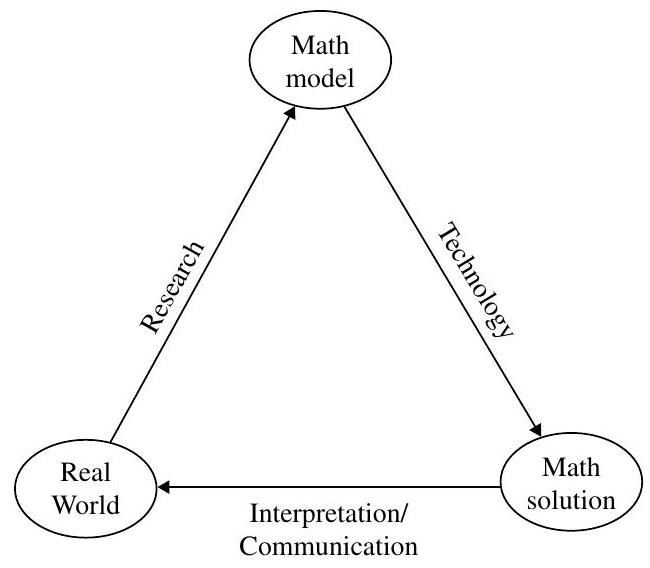
\includegraphics[max width=\textwidth]{2024_04_03_5bb5b4275a64cb9887d1g-354}
\end{center}

Fig. B-1

\section*{TI-89}
The TI-89 Symbolic Manipulation is manufactured by Texas Instruments Incorporated (\href{http://www.ti.com/calc}{http://www.ti.com/calc}). It is hand-held, measuring approximately 7 inches by 3.5 inches, with a depth of nearly an inch. The display screen measures approximately 2.5 inches by 1.5 inches. The TI-89 is powered by four AAA batteries.

Regarding differential equations, the TI-89 can do the following:

\begin{itemize}
  \item Graph slope fields to first-order equations;
  \item Transform higher-order equations into a system of first-order equations;
  \item Runge-Kutta and Euler numerical methods;
  \item Symbolically solve many types of first-order equations;
  \item Symbolically solve many types of second-order equations.
\end{itemize}

\section*{MATHEMATICA}
There are many versions of MATHEMATICA, such as 5.0, 5.1, etc. MATHEMATICA is manufactured by Wolfram Research, Inc. (\href{http://www.wolfram.com/}{http://www.wolfram.com/}). With this package, the user "interacts" with the computer algebra system.

MATHEMATICA is extremely robust. It has the ability to do everything the TI-89 can do. Among its many other capabilities, it has a library of classical functions (e.g. the Hermite polynomials, the Laguerre polynomials, etc.), solves linear difference equations and its graphics powerfully illustrate both curves and surfaces.

\begin{center}
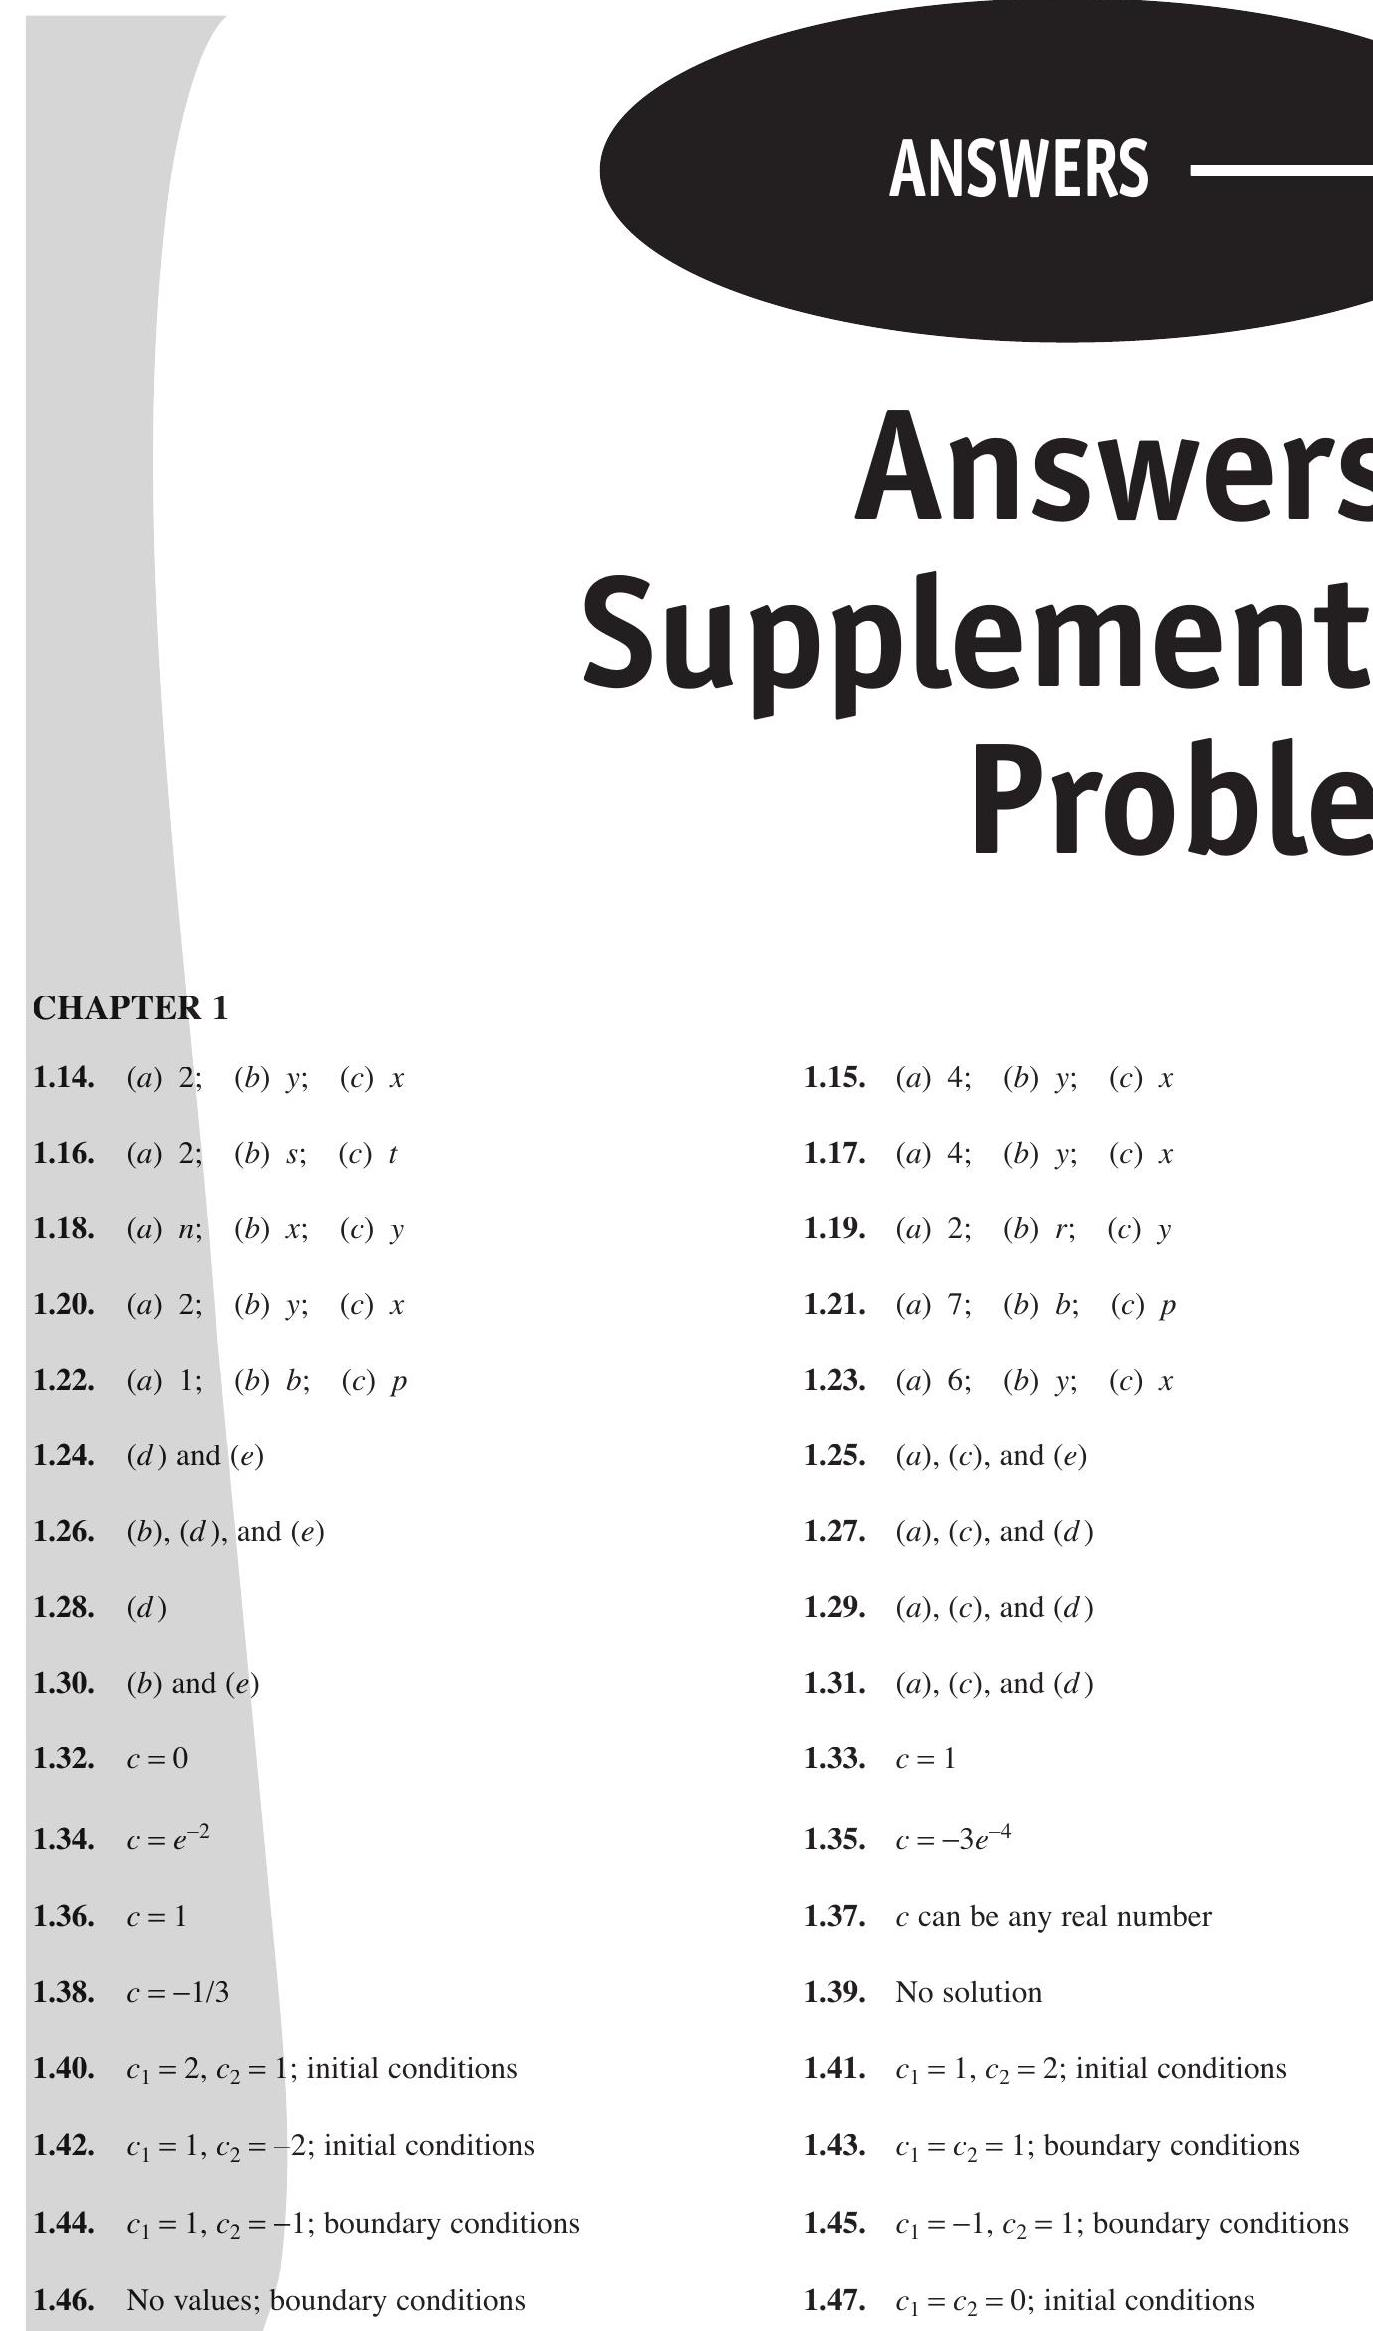
\includegraphics[max width=\textwidth]{2024_04_03_5bb5b4275a64cb9887d1g-356}
\end{center}

1.48. $c_{1}=\frac{-2}{\sqrt{3}-1}, c_{2}=\frac{2}{\sqrt{3}-1} ;$ boundary conditions

1.50. $c_{1}=-2, c_{2}=3$

1.52. $c_{1}=3, c_{2}=-6$

1.54. $c_{1}=1+\frac{3}{e}, c_{2}=-2-\frac{2}{e}$\\
1.49. No values; boundary conditions

1.51. $c_{1}=0, c_{2}=1$

1.53. $c_{1}=0, c_{2}=1$

\section*{CHAPTER 2}
2.12. $T_{C}=\frac{5}{9}\left(T_{F}-32\right)$

2.13. The volume and the temperature are in direct proportion. As one increases, so will the other; as one decreases, so will the other.

2.14. The net force acting on a body is proportional the body's acceleration. This assumes the mass is constant.

2.15. Since $t$ is increasing, and $T(576)=0$, this model is valid for 576 hours. Any time afterwards gives us a negative radicand, and hence, an imaginary answer, thereby rendering the model useless.

2.16. At $t=10$, because $T^{\prime}(10)=0$, and $T^{\prime}(t)>0$ for $t>10$.

2.17. The motion must be periodic, because $\sin 2 t$ is a periodic function of period $\pi$.

2.18. (a) $2 \cos 2 t ; \quad$ (b) $-4 \sin 2 t$\\
2.19. (a) $y$ is a constant;\\
(b) $y$ is increasing;\\
(c) $y$ is decreasing;\\
(d) $y$ is increasing.

2.20. $\frac{d X}{d t}=k(M-X)^{3}$, where $k$ is a negative constant.

2.21. The rates of change of gallons of liquid sugar per hour.

2.22. The rates of change of the vats ( $\mathrm{gal} / \mathrm{hr})$ are affected by the amount of liquid sugar present in the vats, as the equations reflect. The signs and magnitudes of the constants $(a, b, c, d, e$, and $f$ ) will determine whether there is an increase or decrease of sugar, depending on the time. The units for $a, b, c$, and $d$ is ( $1 / \mathrm{hr})$; the units for $e$ and $f$ is (gal/hr).

\section*{CHAPTER 3}
3.15. $y^{\prime}=-y^{2} / x$\\
3.16. $y^{\prime}=x /\left(e^{x}-1\right)$\\
3.17. $y^{\prime}=\left(\sin x-y^{2}-y\right)^{1 / 3}$\\
3.18. Cannot reduce to standard form\\
3.19. $y^{\prime}=-y+\ln x$\\
3.20. $y^{\prime}=2$ and $y^{\prime}=x+y+3$\\
3.21. $y^{\prime}=\frac{y-x}{y^{2}}$\\
3.22. $y^{\prime}=\frac{x+y}{x-y}$\\
3.23. $y^{\prime}=\frac{y-x}{x+y}$\\
3.24. $y^{\prime}=y e^{-x}-e^{x}$

3.25. $y^{\prime}=-1$

3.27. Linear, separable, and exact

3.29. Homogeneous, Bernoulli

3.31. Linear, homogeneous, and exact

3.33. Exact

3.35. Linear and exact

\section*{CHAPTER 4}
4.23. $y= \pm \sqrt{k-x^{2}}, k=2 c$

4.25. $y=(k+3 x)^{-1 / 3}, k=-3 c$

4.27. $y=k x, k= \pm e^{-c}$

4.29. $y=k e^{-x^{2} / 2}, k= \pm e^{c}$

4.31. $y^{3} t^{4}=k e^{y}, k= \pm e^{c}$

4.33. $y=3+2 \tan (2 x+k), k=-2 c$

4.35. $x e^{x} d x-2 y d y=0 ; y= \pm \sqrt{x e^{x}-e^{x}-c}$

4.37. $y=-1 /(x-c)$

4.39. $x=k t, k= \pm e^{c}$

4.41. $y=-\sqrt{2+2 \cos x}$

4.43. $\frac{1}{2} e^{x^{2}}+\frac{1}{6} y^{6}-y=\frac{1}{2}$

4.45. $x=\frac{8}{3}+\frac{4}{3} e^{-3 t}$

4.47. $y=k x^{2}-x$

4.49. Not homogeneous

4.51. $3 y x^{2}-y^{3}=k$

4.53. Not homogeneous\\
3.26. Linear

3.28. Linear

3.30. Homogeneous, Bernoulli, separable, and exact

3.32. Homogeneous

3.34. Bernoulli\\
4.24. $y= \pm\left(k+2 x^{2}\right)^{1 / 4}, k=-4 c$

4.26. $y=-\left(\frac{1}{2} t^{2}+t-c\right)^{-1}$

4.28. $\quad y=\ln \left|\frac{k}{x}\right|, c=\ln |k|$

4.30. $2 t^{3}+6 t+2 y^{3}+3 y^{2}=k, k=6 c$

4.32. $y=\tan (x-c)$

4.34. $\frac{1}{x^{2}} d x-\frac{1}{y} d y=0 ; y=k e^{-1 / x}, k= \pm e^{-c}$

4.36. $y= \pm \sqrt{x^{2}+2 x+k}, k=-2 c$

4.38. $x=-3 /\left(t^{3}+k\right), k=3 c$

4.40. $y=-\frac{3}{5}+k e^{5 t}, k= \pm \frac{1}{5} e^{5 c}$

4.42. $y=e^{-1 / 3\left(x^{3}+3 x+4\right)}$

4.44. $\frac{x^{3}}{3}-x-y-\ln |y|=7$

4.46. $y=x \ln |k / x|$

4.48. $y^{2}=k x^{4}-x^{2}$

4.50. $y^{2}=x^{2}-k x$

4.52. $-2 \sqrt{x / y}+\ln |y|=c$

4.54. $y^{2}=-x^{2}\left(1+\frac{1}{\ln \left|k x^{2}\right|}\right)$

\section*{CHAPTER 5}
5.24. $x y+x^{2} y^{3}+y=c_{2}$

5.26. $y=c_{2} e^{-x^{3}}+\frac{1}{3}$

5.28. $x y=c_{2}$

5.30. $x y \sin x+y=c_{2}$

5.32. $y=c_{2} t^{2}$

5.34. $t^{4} y^{3}-t^{2} y=c_{2}$

5.36. $x=\frac{1}{3} t^{2}-\frac{c_{2}}{t}$

5.38. $x=\frac{k}{1+e^{2 t}}$

5.40. $t \cos x+x \sin t=c_{2}$

5.42. $I(x, y)=\frac{1}{y^{2}} ; c y=x-1$

5.44. $I(x, y)=\frac{1}{(x y)^{3}} ; \frac{1}{y^{2}}=2 x^{2}(x-c)$

5.46. $I(x, y)=e^{x^{3}} ; y=c e^{-x^{3}}+\frac{1}{3}$

5.48. $I(x, y)=\frac{1}{y} ; y^{2}=2\left(c-x^{2}\right)$

5.50. $I(x, y)=y^{2} ; x^{2} y^{4}+\frac{x^{2}}{2}=c$

5.52. $I(x, y)=1$ (the equation is exact) $; \frac{1}{2} x^{2} y^{2}=c$

5.54. $I(x, y)=\frac{1}{(x y)^{2}} ; 3 x^{3} y+2 x y^{4}+k x y=-6$

5.56. $x(t)=\frac{t+\sqrt{t^{2}+16}}{2}$

5.58. $x(t)=\frac{t-\sqrt{t^{2}+120}}{2}$

5.60. $y(x)=-\frac{4}{3} e^{-x^{3}}+\frac{1}{3}$

5.62. $y(t)=-\sqrt{2 t}$

5.64. $x(t)=\frac{1}{3} t^{2}+\frac{14}{3}\left(\frac{1}{t}\right)$\\
5.25. Not exact

5.27. $x^{3} y^{2}+y^{4}=c_{2}$

5.29. Not exact

5.31. $y^{2}=c_{2} t$

5.33. Not exact

5.35. $y=\frac{-1}{t \ln |k t|}$

5.37. $2 t^{3}+6 t x^{2}-3 x^{2}=c_{2}$ or $x= \pm \sqrt{\frac{c_{2}-2 t^{3}}{6 t-3}}$

5.39. Not exact

5.41. $I(x, y)=\frac{-1}{x^{2}} ; y=c x-1$

5.43. $I(x, y)=-\frac{1}{x^{2}+y^{2}} ; y=x \tan (x+c)$

5.45. $I(x, y)=\frac{1}{(x y)^{2}} ; \frac{1}{y}=\frac{1}{3} x^{4}-c x$

5.47. $I(x, y)=e^{-y^{2}} ; y^{2}=\ln |k x|$

5.49. $I(x, y)=y^{2} ; y^{3}=\frac{c}{x}$

5.51. $\quad I(x, y)=\frac{1}{(x y)^{2}} ; \ln |x y|=c-y$

5.53. $I(x, y)=-\frac{1}{x^{2}+y^{2}} ; y=x \tan \left(\frac{1}{2} x^{2}+c\right)$

5.55. $\quad I(x, y)=e^{y^{3} / 3} ; x^{3} y^{2} e^{y^{3} / 3}=c$

5.57. $x(t) \equiv 0$

5.59. $x y+x^{2} y^{3}+y=-135$

5.61. No solution

5.63. $y(t)=-\frac{1}{2} t^{2}$

5.65. $x(t)=\frac{-2\left(1+e^{2}\right)}{1+e^{2 t}}$

\section*{CHAPTER 6}
6.20. $y=c e^{-5 x}$

6.22. $y=c e^{0.01 x}$

6.24. $y=c e^{-x^{3}}$

6.26. $y=c e^{3 x^{5} / 5}$

6.28. $y=c / x^{2}$

6.30. $y=c e^{-2 / x}$

6.32. $y=c e^{7 x}-2 x-\frac{2}{7}$

6.34. $y=c e^{-x^{3 / 3}}+1$

6.36. $y=c+\sin x$

6.38. $y^{2}=1 /\left(2 x+c x^{2}\right)$

6.40. $y=\frac{ \pm 1}{\sqrt{1-c e^{2 x}}}$

6.42. $y=e^{-x} /(c-x)$

6.44. $z=c \sqrt{t}$

6.46. $p=\frac{1}{2} t^{3}+3 t^{2}-2 t \ln |t|+c t$

6.48. $T=(3.2 t+c) e^{-0.04 t}$

6.50. $y=\frac{1}{4}\left(-x^{-2}+x^{2}\right)$

6.52. $y=2 e^{-x^{2}}+x^{2}-1$

6.54. $v=-16 e^{-2 t}+16$

6.56. $N=\frac{1}{3}\left(t^{2}+\frac{40}{t}\right)$\\
6.21. $y=c e^{5 x}$

6.23. $y=c e^{-x^{2}}$

6.25. $y=c e^{x^{3 / 3}}$

6.27. $y=c / x$

6.29. $y=c x^{2}$

6.31. $y=c e^{7 x}-\frac{1}{6} e^{x}$

6.33. $y=c e^{7 x}-\frac{2}{53} \cos 2 x-\frac{7}{53} \sin 2 x$

6.35. $y=c e^{-3 / x}-\frac{1}{3}$

6.37. $\frac{1}{y}=c e^{x}+1$

6.39. $y=\left(6+c e^{-x^{2} / 4}\right)^{2}$

6.41. $y=\left(1+c e^{-3 x}\right)^{1 / 3}$

6.43. $y=c e^{-50 t}$

6.45. $N=c e^{k t}$

6.47. $Q=4(20-t)+c(20-t)^{2}$

6.49. $p=\frac{4}{3} z+c z^{-2}$

6.51. $y=5 e^{-3\left(x^{2}-\pi^{2}\right)}$

6.53. $\frac{1}{y^{4}}=-\frac{31}{16} x^{8}+2 x^{10}$

6.55. $q=\frac{1}{5} e^{-t}+\frac{8}{5} \sin 2 t+\frac{4}{5} \cos 2 t$

6.57. $T=-60 e^{-0.069 t}+30$

\section*{CHAPTER 7}
7.26. (a) $N=250 e^{0.166 t}$\\
(b) $11.2 \mathrm{hr}$\\
7.27. (a) $N=300 e^{0.0912 t}$;\\
(b) $7.6 \mathrm{hr}$\\
7.28.\\
(a) $2.45 \mathrm{oz}$\\
(b) $15.19 \mathrm{oz}$\\
7.29. 32 fold increase\\
7.30. $3.17 \mathrm{hr}$\\
7.31. (a) $N=80 e^{0.0134 t}$ (in millions);\\
(b) 91.5 million

7.32. $\quad N=16,620 e^{0.11 t} ; N_{0}=16,620$

7.34. $\quad N=N_{0} e^{-0.105 t} ; t_{1 / 2}=6.6 \mathrm{hr}$

7.36. $\$ 15,219.62$

7.38. $\$ 14,288.26$

7.40. 10.99 percent

7.42. $7.93 \mathrm{yr}$

7.44. 8.38 yr

7.46. $T=80 e^{-0.035 t} ; T_{0}=80^{\circ} \mathrm{F}$

7.48. (a) $138.6^{\circ} \mathrm{F}$;

(b) $3.12 \mathrm{~min}$

7.50. An additional $1.24 \mathrm{~min}$

7.52. (a) $5.59 \mathrm{sec}$;

(b) $5.59 \mathrm{sec}$

7.54. (a) $32 t+10$;

(b) $5 \mathrm{sec}$

7.56. $\quad 976.6 \mathrm{ft}$

7.58. (a) $v=48-48 e^{-2 t / 3}$;

(b) $x=72 e^{-2 t / 3}+48 t-72$

7.60. $320 \mathrm{ft} / \mathrm{sec}$

7.62. (a) $v=-320 e^{-0.1 t}+320$;

(b) $x=3200 e^{-0.1 t}+320 t-3200$;

(c) $6.9 \mathrm{sec}$

7.64. (a) $v=320-320 e^{-t / 10}$;

(b) $x=3200 e^{-t / 10}+320 t-3200$

7.66. $Q=-\frac{7}{40}(20-t)^{2}+4(20-t)$;

at $t=10, Q=22.5 \mathrm{lb}$

(Note that $a=80(1 / 8)=10 \mathrm{lb}$.)

7.68. $56.3 \mathrm{lb}$

7.70. $80 \mathrm{~g}$\\
7.33. (a) $N=100 e^{-0.026 t}$; (b) $4.05 \mathrm{yr}$

7.35. $\quad N=\frac{500}{1+99 e^{-500 k t}}$

7.37. $\$ 16,904.59$

7.39. 8.67 percent

7.41. $20.93 \mathrm{yr}$

7.43. 12.78 percent

7.45. $T=-100 e^{-0.029 t}+100$;

(a) $23.9 \mathrm{~min}$; (b) $44^{\circ} \mathrm{F}$

7.47. $T=-100 e^{-0.029 t}+150 ; t_{100}=23.9 \mathrm{~min}$

7.49. (a) $113.9^{\circ} \mathrm{F}$; (b) $6.95 \mathrm{~min}$

7.51. (a) $v=32 t$; (b) $16 t^{2}$

7.53. (a) $32 t+30 ;$ (b) $3.49 \mathrm{sec}$

7.55. $31.25 \mathrm{sec}$

7.57. (a) $\frac{d v}{d t}=-g$; (b) $v=-g t+v_{0}$;

(c) $t_{m}=\frac{v_{0}}{g} ;$ (d) $x=-\frac{1}{2} g t^{2}+v_{0} t$;

(e) $x_{m}=\frac{v_{0}^{2}}{2 g}$

7.59. (a) $v=128-118 e^{-t / 4}$;

(b) $6.472 \mathrm{sec}$

7.61. $0.392 \mathrm{~m} / \mathrm{sec}$ with $g=9.8 \mathrm{~m} / \mathrm{sec}^{2}$

7.63. (a) $v=4-4 e^{-8 t}$;

(b) $x=\frac{1}{2} e^{-8 t}+4 t-\frac{1}{2}$

7.65. (a) $Q=-5 e^{-0.2 t}+5$;

(b) $\frac{Q}{V}=\frac{1}{2}\left(-e^{-0.2 t}+1\right)$

7.67. (a) $Q=80 e^{-0.04 t}$;

(b) $17.3 \mathrm{~min}$

7.69. $111.1 \mathrm{~g}$

7.71. (a) $-\frac{99}{2} e^{-10 t} ;$ (b) $0 \mathrm{amp}$

7.72.\\
(a) $q=2+3 e^{-10 t}$;\\
(b) $I=-30 e^{-10 t}$\\
7.73. (a) $q=10 e^{-2.5 t}$;\\
(b) $I=-25 e^{-2.5 t}$

7.74.

(a) $q=\frac{1}{50}\left(2 \sin t-\cos t+e^{-2 t}\right)$;

(b) $I_{s}=\frac{1}{50}(2 \cos t+\sin t)$

7.76.\\
(a) $I=\frac{1}{10}\left(1-e^{-50 t}\right)$;\\
(b) $I_{s}=\frac{1}{10}$

7.78. (a) $I=\frac{1}{10}\left(9+51 e^{-20 t / 3}\right)$;

(b) $I_{t}=\frac{51}{10} e^{-20 t / 3}$

7.80. $A=\frac{2}{\sqrt{34}} \quad \phi=\arctan \frac{3}{5}$

7.82. $x y=k$

7.84. $x^{2} y+\frac{1}{3} y^{3}=k$

7.86. $x^{2}+\frac{1}{2} y^{2}=k(k>0)$

7.88. $N=\frac{1,000,000}{1+999 e^{-0.275 t}}$\\
7.75. (a) $q=\frac{1}{5}\left(\sin 2 t+2 \cos 2 t+23 e^{-4 t}\right)$;

(b) $I_{s}=\frac{1}{5}(2 \cos 2 t-4 \sin 2 t)$

7.77. (a) $I=10 e^{-25 t} ; \quad$ (b) $I_{t}=10 e^{-25 t}$

7.79. $I=\frac{1}{626}\left(e^{-25 t}+25 \sin t-\cos t\right)$

7.81. $A=-\frac{3}{\sqrt{101}} \quad \phi=\arctan 10$

7.83. $y^{2}=-2 x+k$

7.85. $x^{2}+y^{2}=k x$

7.87. $N=\frac{1000}{1+9 e^{-0.1158 t}}$

7.89. $\frac{2+v}{2-v}=3 e^{32 t}$ or $v=2\left(3 e^{32 t}-1\right) /\left(3 e^{32 t}+1\right)$

\section*{CHAPTER 8}
8.33. $(e),(g),(j)$, and $(k)$ are nonlinear; all the rest are linear. Note that $(f)$ has the form $y^{\prime}-(2+x) y=0$.

8.34. (a), (c), and $(f)$ are homogeneous. Note that $(l)$ has the form $y^{\prime \prime}=-e^{x}$.

8.35. (b), (c), and ( $l$ ) have constant coefficients.

8.36. $W=0$

8.37. $W=-x^{2}$; the set is linearly independent.

8.38. $W=-x^{4}$; the set is linearly independent.

8.39. $W=-2 x^{3}$; the set is linearly independent.

8.40. $W=-10 x$; the set is linearly independent.

8.41. $W=0$

8.42. $W=-4$; the set is linearly independent.

8.43. $W=e^{5 x}$; the set is linearly independent.

8.44. $W=0$

8.45. $W=0$

8.46. $W=0$

8.47. $W=2 x^{6}$; the set is linearly independent.

8.48. $W=6 e^{2 x}$; the set is linearly independent.

8.49. $W=0$

8.50. $[4] 3 x+[-3] 4 x \equiv 0$

8.51. $[1] x^{2}+[1]\left(-x^{2}\right) \equiv 0$

8.52. $[5]\left(3 e^{2 x}\right)+[-3]\left(5 e^{2 x}\right) \equiv 0$

8.53. $[-2] x+[7](1)+[1](2 x-7) \equiv 0$

8.54. $[3](x+1)+[-2]\left(x^{2}+x\right)$

$+[1]\left(2 x^{2}-x-3\right) \equiv 0$

8.55. $[-6] \sin x+[-1](2 \cos x)$

$$
+[2](3 \sin x+\cos x) \equiv 0
$$

8.57. $y=c_{1} e^{2 x}+c_{2} e^{3 x}$

8.59. $y=c_{1} e^{8 x}+c_{2}$

8.60. Since $y_{1}$ and $y_{2}$ are linearly dependent, there is not enough information provided to exhibit the general solution.

8.61. $y=c_{1} x+c_{2} e^{x}+c_{3} y_{3}$ where $y_{3}$ is a third particular solution, linearly independent from the other two.

8.62. Since the given set is linearly dependent, not enough information is provided to exhibit the general solution.

8.63. $y=c_{1} e^{-x}+c_{2} e^{x}+c_{3} e^{2 x}$

8.64. $y=c_{1} x^{2}+c_{2} x^{3}+c_{3} x^{4}+c_{4} y_{4}+c_{5} y_{5}$, where $y_{4}$ and $y_{5}$ are two other solutions having the property that the set $\left\{x^{2}, x^{3}\right.$, $\left.x^{4}, y_{4}, y_{5}\right\}$ is linearly independent.

8.65. $y=c_{1} \sin x+c_{2} \cos x+x^{2}-2$

8.66. Since $e^{x}$ and $3 e^{x}$ are linearly dependent, there is not enough information given to find the general solution.

8.67. $y=c_{1} e^{x}+c_{2} e^{-x}+c_{3} x e^{x}+5$

8.68. Theorem 8.1 does not apply, since $a_{0}(x)=-(2 / x)$ is not continuous about $x_{0}=0$.

8.69. Yes; $a_{0}(x)$ is continuous about $x_{0}=1$.

8.70. Theorem 8.1 does not apply, since $b_{1}(x)$ is zero at the origin.

\section*{CHAPTER 9}
9.17. $y=c_{1} e^{x}+c_{2} e^{-x}$\\
9.18. $y=c_{1} e^{-5 x}+c_{2} e^{6 x}$\\
9.19. $y=c_{1} e^{x}+c_{2} x e^{x}$\\
9.20. $y=c_{1} \cos x+c_{2} \sin x$\\
9.21. $y=c_{1} e^{-x} \cos x+c_{2} e^{-x} \sin x$\\
9.22. $y=c_{1} e^{\sqrt{7} x}+c_{2} e^{-\sqrt{7} x}$\\
9.23. $y=c_{1} e^{-3 x}+c_{2} x e^{-3 x}$\\
9.24. $y=c_{1} e^{-x} \cos \sqrt{2} x+c_{2} e^{-x} \sin \sqrt{2} x$\\
9.25. $y=c_{1} e^{[(3+\sqrt{29}) / 2] x}+c_{2} e^{[(3-\sqrt{29}) / 2] x}$\\
$=e^{(3 / 2) x}\left(k_{1} \cosh \frac{\sqrt{29}}{2} x+k_{2} \sinh \frac{\sqrt{29}}{2} x\right)$\\
9.26. $y=c_{1} e^{-(1 / 2) x}+c_{2} x e^{-(1 / 2) x}$

9.27. $x=c_{1} e^{4 t}+c_{2} e^{16 t}$

9.28. $x=c_{1} e^{-50 t}+c_{2} e^{-10 t}$

9.29. $x=c_{1} e^{(3+\sqrt{5}) t / 2}+c_{2} e^{(3-\sqrt{5}) t / 2}$

9.30. $x=c_{1} e^{5 t}+c_{2} t e^{5 t}$

9.31. $x=c_{1} \cos 5 t+c_{2} \sin 5 t$

9.32. $x=c_{1}+c_{2} e^{-25 t}$

9.33. $x=c_{1} e^{-t / 2} \cos \frac{\sqrt{7}}{2} t+c_{2} e^{-t / 2} \sin \frac{\sqrt{7}}{2} t$

9.35. $u=c_{1} e^{(2+\sqrt{2}) t}+c_{2} e^{(2-\sqrt{2}) t}$

9.37. $u=c_{1} e^{6 t}+c_{2} e^{-6 t}=k_{1} \cosh 6 t+k_{2} \sinh 6 t$

9.39. $Q=c_{1} e^{(7+\sqrt{29}) t / 2}+c_{2} e^{(7-\sqrt{29}) t 2}$

9.41. $\quad P=c_{1} e^{-x} \cos 2 \sqrt{2} x+c_{2} e^{-x} \sin 2 \sqrt{2} x$

9.43. $N=c_{1} e^{-5 x / 2} \cos \frac{\sqrt{71}}{2} x+c_{2} e^{-5 x / 2} \sin \frac{\sqrt{71}}{2} x$

9.45. $R=c_{1}+c_{2} e^{-5 \theta}$

\section*{CHAPTER 10}
10.16. $y=c_{1} e^{-x}+c_{2} e^{x}+c_{3} e^{2 x}$

10.18. $y=c_{1} e^{x}+c_{2} x e^{x}+c_{3} x^{2} e^{x}$

10.20. $y=\left(c_{1}+c_{2} x\right) \cos x+\left(c_{3}+c_{4} x\right) \sin x$

10.22. $y=c_{1} e^{x}+c_{2} e^{-x}+c_{3} x e^{-x}+c_{4} x^{2} e^{-x}$

10.24. $y=c_{1}+c_{2} x+c_{3} x^{2}+c_{4} e^{-5 x}$

10.26. $y=c_{1} e^{2 x} \cos 2 x+c_{2} e^{2 x} \sin 2 x+c_{3} e^{-2 x}$ $+c_{4} x e^{-2 x}+c_{5} e^{x}+c_{6} e^{-x}$

10.28. $x=c_{1}+c_{2} t+c_{3} t^{2}$

10.30. $x=c_{1} e^{5 t}+c_{2} \cos 5 t+c_{3} \sin 5 t$

10.32. $q=c_{1} e^{x}+c_{2} e^{-x}+c_{3} e^{\sqrt{2} x}+c_{4} e^{-\sqrt{2} x}$

10.34. $r=c_{1} e^{-\theta}+c_{2} \theta e^{-\theta}+c_{3} \theta^{2} e^{-\theta}+c_{4} \theta^{3} e^{-\theta}+c_{5} \theta^{4} e^{-\theta}$

10.36. $y=c_{1}+c_{2} \cos 19 x+c_{3} \sin 19 x$

10.38. $y=c_{1} e^{2 x} \cos 9 x+c_{2} e^{2 x} \sin 9 x$

$$
+c_{3} x e^{2 x} \cos 9 x+c_{4} x e^{2 x} \sin 9 x
$$

10.40. $y=c_{1} \cos 6 x+c_{2} \sin 6 x+c_{3} x \cos 6 x$ $+c_{4} x \sin 6 x+c_{5} x^{2} \cos 6 x+c_{6} x^{2} \sin 6 x$

10.42. $y^{\prime \prime \prime}+4 y^{\prime \prime}-124 y^{\prime}+224 y=0$\\
9.34. $u=c_{1} e^{t} \cos \sqrt{3} t+c_{2} e^{t} \sin \sqrt{3} t$

9.36. $u=c_{1}+c_{2} e^{36 t}$

9.38. $Q=c_{1} e^{5 t / 2} \cos \frac{\sqrt{3}}{2} t+c_{2} e^{5 t / 2} \sin \frac{\sqrt{3}}{2} t$

9.40. $P=c_{1} e^{9 t}+c_{2} t e^{9 t}$

9.42. $N=c_{1} e^{3 x}+c_{2} e^{-8 x}$

9.44. $T=c_{1} e^{-15 \theta}+c_{2} \theta e^{-15 \theta}$

10.17. $y=c_{1} e^{x}+c_{2} x e^{x}+c_{3} e^{-x}$

10.19. $y=c_{1} e^{x}+c_{2} \cos x+c_{3} \sin x$

10.21. $y=c_{1} e^{x}+c_{2} e^{-x}+c_{3} \cos x+c_{4} \sin x$

10.23. $y=c_{1} e^{-2 x}+c_{2} x e^{-2 x}+c_{3} e^{2 x} \cos 2 x+c_{4} e^{2 x} \sin 2 x$

10.25. $y=\left(c_{1}+c_{3} x\right) e^{-(1 / 2) x} \cos \frac{\sqrt{3}}{2} x$

$$
+\left(c_{2}+c_{4} x\right) e^{-(1 / 2) x} \sin \frac{\sqrt{3}}{2} x
$$

10.27. $x=c_{1} e^{-t}+c_{2} t e^{-t}+c_{3} t^{2} e^{-t}+c_{4} t^{3} e^{-t}$

10.29. $x=c_{1} \cos t+c_{2} \sin t+c_{3} \cos 3 t+c_{4} \sin 3 t$

10.31. $q=c_{1} e^{x}+c_{2} e^{-x}+c_{3} \cos \sqrt{2} x+c_{4} \sin \sqrt{2} x$

10.33. $\quad N=c_{1} e^{-6 x}+c_{2} e^{8 x}+c_{3} e^{10 x}$

10.35. $y=c_{1} e^{2 x}+c_{2} e^{8 x}+c_{3} e^{-14 x}$

10.37. $y=c_{1}+c_{2} x+c_{3} e^{2 x} \cos 9 x+c_{4} e^{2 x} \sin 9 x$

10.39. $y=c_{1} e^{5 x}+c_{2} x e^{5 x}+c_{3} x^{2} e^{5 x}+c_{4} e^{-5 x}$

$$
+c_{5} x e^{-5 x}
$$

10.41. $y=e^{-3 x}\left(c_{1} \cos x+c_{2} \sin x+c_{3} x \cos x\right.$

$$
\left.+c_{4} x \sin x\right)+e^{3 x}\left(c_{5} \cos x+c_{6} \sin x\right.
$$

$$
\left.+c_{7} x \cos x+c_{8} x \sin x\right)
$$

10.43. $y^{\prime \prime \prime}+361 y^{\prime}=0$

10.44. $y^{(4)}-4 y^{\prime \prime \prime}+85 y^{\prime \prime}=0$

10.46. $y^{(5)}-5 y^{(4)}-50 y^{(3)}+250 y^{\prime \prime}+625 y^{\prime}-3125 y=0$

10.48. $y=c_{1} \cos 4 x+c_{2} \sin 4 x+c_{3} \cos 3 x+c_{4} \sin 3 x$ 10.50. $y=c_{1} e^{2 x}+c_{2} x e^{2 x}+c_{3} e^{5 x}+c_{4} x e^{5 x}$\\
10.45. $y^{(4)}-8 y^{\prime \prime \prime}+186 y^{\prime \prime}-680 y^{\prime}+7225 y=0$

10.47. $y=c_{1} e^{-x}+c_{2} x e^{-x}+c_{3} x^{2} e^{-x}+c_{4} x^{3} e^{-x}$

10.49. $y=c_{1} \cos 4 x+c_{2} \sin 4 x+c_{3} x \cos 4 x+c_{4} x \sin 4 x$

\section*{CHAPTER 11}
11.15. $y_{p}=A_{1} x+A_{0}$

11.17. $y_{p}=A_{2} x^{2}+A_{1} x+A_{0}$

11.19. $y_{p}=A e^{5 x}$

11.21. $y_{p}=A \sin 3 x+B \cos 3 x$

11.23. $y_{p}=\left(A_{1} x+A_{0}\right) \sin 3 x+\left(B_{1} x+B_{0}\right) \cos 3 x$

11.25. $y_{p}=\left(A_{1} x+A_{0}\right) e^{5 x}$

11.27. $y_{p}=A e^{3 x}$

11.29. $y_{p}=A e^{5 x}$

11.31. $y_{p}=A \sin \sqrt{2} x+B \cos \sqrt{2} x$

11.33. $y_{p}=A \sin 3 x+B \cos 3 x$

11.35. $y_{p}=A e^{-x} \sin 3 x+B e^{-x} \cos 3 x$

11.37. $x_{p}=t\left(A_{1} t+A_{0}\right)$

11.39. $x_{p}=\left(A_{1} t+A_{0}\right) e^{-2 t}+B t$

11.41. $x_{p}=t^{2}\left(A_{1} t+A_{0}\right) e^{t}$

11.43. $x_{p}=\left(A_{1} t+A_{0}\right) e^{2 t} \sin 3 t$

$$
+\left(B_{1} t+B_{0}\right) e^{2 t} \cos 3 t
$$

11.45. $y=c_{1} e^{x}+c_{2} x e^{x}+3 e^{2 x}$

11.47. $y=c_{1} e^{x}+c_{2} x e^{x}+\frac{3}{2} x^{2} e^{x}$

11.49. $y=c_{1} e^{x}+x e^{x}$

11.51. $y=c_{1} e^{x}-\frac{1}{2} \sin x-\frac{1}{2} \cos x$

$$
+\frac{2}{5} \sin 2 x-\frac{1}{5} \cos 2 x
$$

11.16. $y_{p}=A_{2} x^{2}+A_{1} x+A_{0}$

11.18. $y_{p}=A e^{-2 x}$

11.20. $y_{p}=A x e^{2 x}$

11.22. $y_{p}=A \sin 3 x+B \cos 3 x$

11.24. $y_{p}=A_{1} x+A_{0}+B e^{8 x}$

11.26. $y_{p}=x\left(A_{1} x+A_{0}\right) e^{3 x}$

11.28. $y_{p}=\left(A_{1} x+A_{0}\right) e^{3 x}$

11.30. $y_{p}=\left(A_{2} x^{2}+A_{1} x+A_{0}\right) e^{5 x}$

11.32. $y_{p}=\left(A_{2} x^{2}+A_{1} x+A_{0}\right) \sin \sqrt{2} x$

$$
+\left(B_{2} x^{2}+B_{1} x+B_{0}\right) \cos \sqrt{2} x
$$

11.34. $y_{p}=A \sin 4 x+B \cos 4 x+C \sin 7 x+D \cos 7 x$

11.36. $y_{p}=x\left(A e^{5 x} \sin 3 x+B e^{5 x} \cos 3 x\right)$

11.38. $x_{p}=t\left(A_{2} t^{2}+A_{1} t+A_{0}\right)$

11.40. $x_{p}=t^{2}\left(A e^{t}\right)$

11.42. $x_{p}=A t+\left(B_{1} t+B_{0}\right) \sin t+\left(C_{1} t+C_{0}\right) \cos t$

11.44. $y=c_{1} e^{x}+c_{2} x e^{x}+x^{2}+4 x+5$

11.46. $y=c_{1} e^{x}+c_{2} x e^{x}-2 \sin x$

11.48. $y=c_{1} e^{x}+c_{2} x e^{x}+\frac{1}{6} x^{3} e^{x}$

11.50. $y=c_{1} e^{x}+x e^{2 x}-e^{2 x}-1$

11.52. $y=c_{1} e^{x}+c_{2} x e^{x}+c_{3} x^{2} e^{x}+\frac{1}{6} x^{3} e^{x}-1$

\section*{CHAPTER 12}
12.9. $\quad y=c_{1} e^{x}+c_{2} x e^{x}+\frac{1}{12} x^{-3} e^{x}$

12.11. $y=c_{1} e^{-x}+c_{2} e^{2 x}+\frac{1}{4} e^{3 x}$

12.13. $y=c_{3}+c_{2} e^{7 x}+\frac{3}{7} x$

$$
\left(\text { with } c_{3}=c_{1}+\frac{3}{49}\right)
$$

12.15. $y=c_{1}+c_{2} x^{2}+x e^{x}-e^{x}$

12.17. $y=c_{1} e^{-x^{2}}+\frac{1}{2}$

12.19. $x=c_{1} e^{t}+c_{2} t e^{t}+\frac{e^{t}}{2 t}$

12.21. $x=c_{1} \cos 2 t+c_{2} \sin 2 t-1$

$+(\sin 2 t) \ln |\sec 2 t+\tan 2 t|$

12.23. $x=c_{1} t+c_{2}\left(t^{2}+1\right)+\frac{t^{4}}{6}-\frac{t^{2}}{2}$

12.25. $r=c_{1} e^{t}+c_{2} t e^{t}+c_{3} t^{2} e^{t}+\frac{t^{2}}{2} e^{t} \ln |t|$

12.27. $r=c_{1} e^{5 t}+c_{2} \cos 5 t+c_{3} \sin 5 t-8$

12.29. $y=\frac{c_{1}}{t}+c_{2}+c_{3} t-\ln |t|$

\section*{CHAPTER 13}
13.7. $y=\frac{1}{12} e^{-x}+\frac{2}{3} e^{2 x}+\frac{1}{4} e^{3 x}$

13.9. $y=e^{-x}+e^{2 x}$

13.11. $y=-\cos 1 \cos x-\sin 1 \sin x+x$ $=-\cos (x-1)+x$\\
12.10. $y=c_{1} \cos x+c_{2} \sin x+(\cos x) \ln |\cos x|+x \sin x$

12.12. $y=c_{1} e^{30 x}+c_{2} x e^{30 x}+\frac{1}{80} e^{10 x}$

12.14. $y=c_{1} x+\frac{c_{2}}{x}+\frac{x^{2}}{3} \ln |x|-\frac{4}{9} x^{2}$

12.16. $y=c_{1} x+\frac{1}{2} x^{3}$

12.18. $y=c_{1}+c_{2} x+c_{3} x^{2}+2 x^{3}$

12.20. $x=c_{3} e^{3 t}+c_{2} t e^{3 t}-e^{3 t} \ln |t| \quad\left(\right.$ with $\left.c_{3}=c_{1}-1\right)$

12.22. $x=c_{3} e^{t}+c_{4} e^{3 t}+\frac{e^{t}}{2} \ln \left(1+e^{-t}\right)$

$$
\begin{aligned}
& -\frac{e^{3 t}}{2} \ln \left(1+e^{-t}\right)+\frac{e^{2 t}}{2} \\
& \left(\text { with } c_{3}=c_{1}-\frac{1}{4} ; c_{4}=c_{2}+\frac{3}{4}\right)
\end{aligned}
$$

12.24. $x=c_{1} e^{t}+\frac{c_{2}}{t}-\frac{t^{2}}{3}-t-1$

12.26. $r=c_{1} e^{-2 t}+c_{2} t e^{-2 t}+c_{3} t^{2} e^{-2 t}+2 t^{3} e^{-2 t}$

12.28. $z=c_{1}+c_{2} e^{\theta}+c_{3} e^{2 \theta}$

$$
+\frac{1}{4}\left(1+e^{\theta}\right)^{2}\left[-3+2 \ln \left(1+e^{\theta}\right)\right]
$$

12.30. $y=c_{1}+c_{2} x+c_{3} x^{2}+c_{6} e^{2 x}+c_{5} e^{-2 x}+x e^{2 x}$

$$
\left(\text { with } c_{6}=c_{4}-\frac{7}{4}\right)
$$

13.8. $y=\frac{13}{12} e^{-x}+\frac{2}{3} e^{2 x}+\frac{1}{4} e^{3 x}$

13.10. $y=\left(1+\frac{1}{12} e^{3}\right) e^{-(x-1)}$

$$
+\left(1-\frac{1}{3} e^{3}\right) e^{2(x-1)}+\frac{1}{4} e^{3 x}
$$

13.12. $y=-\frac{1}{6} \cos 2 x+\frac{1}{4} \cos ^{2} 2 x$

$$
\begin{aligned}
& -\frac{1}{12} \cos ^{4} 2 x+\frac{1}{12} \sin ^{4} 2 x \\
= & \frac{1}{12}\left(1+\cos ^{2} 2 x-2 \cos 2 x\right)
\end{aligned}
$$

13.13. $y \equiv 0$

13.15. $y=e^{-t}\left(\frac{3}{10} \cos t+\frac{11}{10} \sin t\right)+\frac{1}{10} \sin 2 t-\frac{3}{10} \cos 2 t$

\section*{CHAPTER 14}
14.26. $60 \mathrm{lb} / \mathrm{ft}$

14.28. 130.7 dynes/ $/ \mathrm{cm}$

14.30. $x=\frac{1}{6} \cos 8 t$

14.32. $x=3 \cos 12 t+\frac{5}{6} \sin 12 t$

14.34. (a) $\omega=8 \mathrm{Hz;}$ (b) $f=4 / \pi \mathrm{Hz}$; (c) $T=\pi / 4 \mathrm{sec}$

14.36. (a) $\omega=2 \mathrm{~Hz}$;

(b) $f=1 / \pi \mathrm{Hz}$;

(c) $T=\pi \mathrm{sec}$

14.38. $x=-\frac{1}{3} \sqrt{3} e^{-4 t} \sin 4 \sqrt{3} t$

14.40. $x=\frac{3}{4} e^{-2 t}-\frac{1}{4} e^{-6 t}$

14.42. $x=-0.1 e^{-4 t} \cos \sqrt{0.02} t$

$$
-\frac{2.4}{\sqrt{0.02}} e^{-4 t} \sin \sqrt{0.02} t
$$

14.44. $x=e^{-2 t}\left(\frac{2}{5} \cos 2 t-\frac{6}{5} \sin 2 t\right)$

$$
+\frac{4}{5} \sin 4 t-\frac{2}{5} \cos 4 t
$$

14.46. $x=\frac{1}{16} \sin 4 t-\frac{1}{2} \cos 4 t-\frac{t}{4} \cos 4 t$

14.48. $x=-\frac{5}{4} e^{-2 t} \cos 4 t-\frac{3}{4} e^{-2 t} \sin 4 t$

$$
+\frac{1}{2} \cos 2 t+\frac{1}{4} \sin 2 t
$$

14.50. $x=-4 e^{-3 t} \cos \sqrt{3} t-6 \sqrt{3} e^{-3 t} \sin \sqrt{3} t$

$$
+4 \cos 3 t+2 \sin 3 t
$$

14.52. $q=\frac{1}{100}\left(3 e^{-50 t}-15 e^{-10 t}+12\right)$;

$$
I=\frac{3}{2}\left(e^{-10 t}-e^{-50 t}\right)
$$

13.14. $y=-2+6 x-6 x^{2}+2 x^{3}$

14.27. $17.07 \mathrm{lb} / \mathrm{ft}$

14.29. $19.6 \mathrm{~N} / \mathrm{m}$

14.31. $x=-\frac{1}{6} \cos 8 t+\frac{1}{4} \sin 8 t$

14.33. $x=\sin 2 t-\cos 2 t$

14.35. (a) $\omega=12 \mathrm{Hz;}$ (b) $f=6 / \pi \mathrm{Hz;}$ (c) $T=\pi / 6 \mathrm{sec}$

14.37. $x=x_{0} \cos \sqrt{k / m} t+v_{0} \sqrt{m / k} \sin \sqrt{k / m} t$

14.39. $x=-\frac{1}{2} e^{-4 t}-2 t e^{-4 t}$

14.41. $x=-0.1 \mathrm{e}^{-4 t}-2.4 t e^{-4 t}$

14.43. $x=-8.535 e^{-3.859}+8.435 e^{-4.141}$

14.45. $x=-\frac{4}{105} \sin 5 t+\frac{2}{21} \sin 2 t$

14.47. $x=e^{-4 t} \cos 4 \sqrt{3} t-\cos 8 t$

14.49. $x_{s}=\frac{1}{2} \cos 2 t+\frac{1}{4} \sin 2 t=\frac{\sqrt{5}}{4} \cos (2 t-0.46)$

14.51. $x_{s}=4 \cos 3 t+2 \sin 3 t=\sqrt{20} \cos (3 t-0.46)$

14.53. $I=10.09 e^{-50 t} \sin 50 \sqrt{19} t ; q=\frac{11}{250}$

$$
\left(1-e^{-50 t} \cos 50 \sqrt{19} t-\frac{1}{\sqrt{19}} e^{-50 t} \sin 50 \sqrt{19} t\right)
$$

14.54. $\quad I=\frac{5}{4}\left(e^{-50 t}-e^{-10 t}\right)$

14.56. $I=-\frac{2}{5} e^{-4 t} \cos 6 t+\frac{82}{15} e^{-4 t} \sin 6 t$

$$
+\frac{2}{5} \cos 2 t-\frac{6}{5} \sin 2 t
$$

14.58. $I=-\frac{150}{52} e^{-4 t} \cos 3 t-\frac{425}{52} e^{-4 t} \sin 3 t$

$$
+\frac{150}{52} \cos 3 t+\frac{225}{52} \sin 3 t
$$

14.60. $I=-e^{-200 t} \cos 400 t+\frac{11}{2} e^{-200 t} \sin 400 t$

$$
+\cos 200 t-2 \sin 200 t
$$

14.62. $q=\frac{30}{61} e^{-10 t} \cos 50 t+\frac{36}{61} e^{-10 t} \sin 50 t$

$$
-\frac{30}{61} \cos 60 t-\frac{25}{61} \sin 60 t
$$

14.64. 0

14.66. $\quad 1.28 \mathrm{ft}=15.36$ in submerged

14.68. $x=-0.260 \cos (5 t-0.876)$

14.70. $x=-0.236 \cos 6.47 t$\\
14.72.\\
(a) $\omega=5 \mathrm{~Hz}$\\
(c) $T=2 \pi / 5 \mathrm{sec}$\\
(b) $f=5 /(2 \pi) \mathrm{Hz}$

14.74. No equilibrium position; it sinks.

14.76. $x=-4.80 \sin 10.42 t$

14.78. $0.236 \mathrm{ft}=2.84$ in

14.80. $\ddot{x}+\frac{w l \rho}{m} x=0$\\
14.55. $I=24 t e^{-500 t}$

14.57. $I_{s}=\frac{2}{5} \cos 2 t-\frac{6}{5} \sin 2 t=\frac{\sqrt{40}}{5} \cos (2 t+1.25)$

14.59. $I_{s}=\frac{150}{52} \cos 3 t+\frac{225}{52} \sin 3 t$

$$
=5.2 \cos (3 t-0.983)
$$

14.61. $I_{s}=\cos 200 t-2 \sin 200 t$

$$
=\sqrt{5} \cos (200 t+1.11)
$$

14.63. $q_{s}=-\frac{30}{61} \cos 60 t-\frac{25}{61} \sin 60 t$

$$
=-0.64 \cos (60 t-0.69)
$$

14.65. $\frac{1}{640,001}(6392 \cos t+320 \sin t)$

14.67. $x=-\frac{1}{6} \cos 5 t-\frac{1}{5} \sin 5 t$

14.69. $0.764 \mathrm{ft}$ submerged

14.71. (a) $\omega=6.47 \mathrm{Hz;}$ (b) $f=1.03 \mathrm{~Hz}$;

(c) $T=0.97 \mathrm{sec}$

14.73. No equilibrium position; it sinks.

14.75. $9.02 \mathrm{~cm}$ submerged

14.77. $x=c_{1} \cos \sqrt{\frac{\pi \rho r^{2}}{m}} t+c_{2} \sin \sqrt{\frac{\pi \rho r^{2}}{m}} t ;$

$$
T=\frac{2}{r} \sqrt{\frac{\pi m}{\rho}}
$$

14.79. $\quad 159.15 \mathrm{lb}$

14.81. (a) $T=2 \pi \sqrt{\frac{m}{w l \rho}} ;$ (b) period is reduced by $1 / \sqrt{2}$

\section*{CHAPTER 15}
15.18. $\left[\begin{array}{ll}3 & -1 \\ 2 & -1\end{array}\right]$

15.20. $\left[\begin{array}{rrr}2 & 5 & -2 \\ -3 & -3 & -1 \\ -1 & 1 & -3\end{array}\right]$\\
15.19. $\left[\begin{array}{rr}4 & 17 \\ -9 & -8\end{array}\right]$

15.21. $\left[\begin{array}{rrr}11 & 10 & 10 \\ 1 & -6 & 5 \\ 12 & 2 & 22\end{array}\right]$

15.22. Not defined

15.24. (a) $\left[\begin{array}{cc}11 & -5 \\ -7 & 2\end{array}\right]$ (b) $\left[\begin{array}{cc}6 & 11 \\ 5 & 7\end{array}\right]$

15.26. $\left[\begin{array}{rr}2 & 3 \\ -1 & -2\end{array}\right]$

15.28. (a) $\left[\begin{array}{rrr}8 & 0 & 11 \\ -5 & 0 & -7 \\ 4 & 0 & 7\end{array}\right]$ (b) $\left[\begin{array}{rrr}5 & 7 & 2 \\ 4 & 6 & 1 \\ 10 & 14 & 4\end{array}\right]$

15.30. Not defined

15.32. $\lambda^{2}-1=0 ; \lambda_{1}=1, \lambda_{2}=-1$

15.34. $\quad \lambda^{2}-2 \lambda-1=0 ; \lambda_{1}=1+\sqrt{2}, \lambda_{2}=1-\sqrt{2}$

15.36. $\lambda^{2}-10 \lambda+24=0 ; \lambda_{1}=4, \lambda_{2}=6$

15.38. $(-\lambda)\left(\lambda^{2}-5 \lambda\right)=0 ; \lambda_{1}=0, \lambda_{2}=0, \lambda_{3}=5$

The eigenvalue $\lambda=0$ has multiplicity two, while $\lambda=5$ has multiplicity one.

15.40. $(5 t-\lambda)\left(\lambda^{2}-25 t^{2}\right)=0 ; \lambda_{1}=5 t, \lambda_{2}=5 t, \lambda_{3}=-5 t$

15.42. $\left[\begin{array}{c}-2 \sin 2 t \\ \left(1+6 t^{2}\right) e^{3 t^{2}}\end{array}\right]$\\
15.23. Not defined

15.25. $\left[\begin{array}{ll}1 & 0 \\ 0 & 1\end{array}\right]=\mathbf{I}$

15.27. $\left[\begin{array}{rr}-11 & -8 \\ 6 & -11\end{array}\right]$

15.29. (a) $\left[\begin{array}{r}-4 \\ 3\end{array}\right]$ (b) Not defined

15.31. $\left[\begin{array}{c}13 \\ -2 \\ 14\end{array}\right]$

15.33. $\lambda^{2}-2 \lambda+13=0 ; \lambda_{1}=1+2 \sqrt{3} i$,

$$
\lambda_{2}=1-2 \sqrt{3} i
$$

15.35. $\lambda^{2}-9=0 ; \lambda_{1}=3, \lambda_{2}=-3$

15.37. $(1-\lambda)\left(\lambda^{2}+1\right)=0 ; \lambda_{1}=1, \lambda_{2}=-i, \lambda_{3}=-i$

Each eigenvalue has multiplicity one.

15.39. $\lambda^{2}-3 t \lambda+t^{2}=0 ; \lambda_{1}=\left(\frac{3}{2}+\frac{1}{2} \sqrt{5}\right) t$,

$$
\lambda_{2}=\left(\frac{3}{2}-\frac{1}{2} \sqrt{5}\right) t
$$

15.41. $\left[\begin{array}{cc}1 & 2 t \\ 0 & 2\end{array}\right]$

15.43. $\left[\begin{array}{c}\frac{1}{2} \sin 2 \\ \frac{1}{6}\left(e^{3}-1\right)\end{array}\right]$

\section*{CHAPTER 16}
16.13. $\quad \lambda_{1}=2 t, \lambda_{2}=-3 t ;\left[\begin{array}{cc}e^{2 t} & 0 \\ 0 & e^{-3 t}\end{array}\right]$

16.14. $\lambda_{1}=-t, \lambda_{2}=5 t$;

$$
\frac{1}{6}\left[\begin{array}{ll}
4 e^{5 t}+2 e^{-t} & 2 e^{5 t}-2 e^{-t} \\
4 e^{5 t}-4 e^{-t} & 2 e^{5 t}+4 e^{-t}
\end{array}\right]
$$

16.15. $\quad \lambda_{1}=t, \lambda_{2}=-t ;\left[\begin{array}{cc}3 e^{t}-2 e^{-t} & 3 e^{t}-3 e^{-t} \\ -2 e^{t}+2 e^{-t} & -2 e^{t}+3 e^{-t}\end{array}\right]$

16.16. $\lambda_{1}=2 t, \lambda_{2}=-4 t$;

$$
\frac{1}{6}\left[\begin{array}{cc}
4 e^{2 t}+2 e^{-4 t} & e^{2 t}-e^{-4 t} \\
8 e^{2 t}-8 e^{-4 t} & 2 e^{2 t}+4 e^{-4 t}
\end{array}\right]
$$

16.17. $\lambda_{1}=-2 t, \lambda_{2}=-7 t$;

$$
\frac{1}{5}\left[\begin{array}{cc}
7 e^{-2 t}-2 e^{-7 t} & e^{-2 t}-e^{-7 t} \\
-14 e^{-2 t}+14 e^{-7 t} & -2 e^{-2 t}+7 e^{-7 t}
\end{array}\right]
$$

16.18. $\quad \lambda_{1}=\lambda_{2}=2 t ; e^{2 t}\left[\begin{array}{ll}1 & 0 \\ 0 & 1\end{array}\right]$

16.19. $\quad \lambda_{1}=\lambda_{2}=2 t ; e^{2 t}\left[\begin{array}{ll}1 & t \\ 0 & 1\end{array}\right]$

16.21. $\lambda_{1}=4 i t, \lambda_{2}=-4 i t ; \frac{1}{4}\left[\begin{array}{cc}4 \cos 2 t & \sin 4 t \\ -16 \sin 4 t & 4 \cos 4 t\end{array}\right]$

16.23. $\lambda_{1}=\lambda_{2}=-2 t ; e^{-2 t}\left[\begin{array}{cc}1+2 t & t \\ -4 t & 1-2 t\end{array}\right]$

16.25. $\lambda_{1}=(-4+3 i) t, \lambda_{2}=(-4-3 i) t ; \frac{e^{-4 t}}{3}\left[\begin{array}{cc}3 \cos 3 t+4 \sin 3 t & \sin 3 t \\ -25 \sin 3 t & 3 \cos 3 t-4 \sin 3 t\end{array}\right]$

16.26. $\lambda_{1}=(3+\sqrt{15} i) t, \lambda_{2}=(3-\sqrt{15} i) t ; \frac{e^{3 t}}{\sqrt{15}}\left[\begin{array}{cc}\sqrt{15} \cos \sqrt{15} t+\sin \sqrt{15} t & -2 \sin \sqrt{15} t \\ 8 \sin \sqrt{15} t & \sqrt{15} \cos \sqrt{15} t-\sin \sqrt{15} t\end{array}\right]$

16.27. $\lambda_{1}=\lambda_{2}=\lambda_{3}=2 t ; e^{2 t}\left[\begin{array}{ccc}1 & t & t^{2} / 2 \\ 0 & 1 & t \\ 0 & 0 & 1\end{array}\right]$

16.28. $\lambda_{1}=\lambda_{2}=\lambda_{3}=2 t ; e^{2 t}\left[\begin{array}{ccc}1 & 0 & 0 \\ 0 & 1 & t \\ 0 & 0 & 1\end{array}\right]$

16.29. $\lambda_{1}=-t, \lambda_{2}=\lambda_{3}=2 t$;

$$
\frac{1}{9}\left[\begin{array}{ccc}
9 e^{-t} & -3 e^{-t}+3 e^{2 t} & e^{-t}-e^{2 t}+3 t e^{2 t} \\
0 & 9 e^{2 t} & 9 t e^{2 t} \\
0 & 0 & 9 e^{2 t}
\end{array}\right]
$$

16.30. $\lambda_{1}=\lambda_{2}=\lambda_{3}=0 ;\left[\begin{array}{ccc}1 & 0 & 0 \\ 0 & 1 & 0 \\ 0 & 0 & 1\end{array}\right]$

(see Problem 16.12)

16.31. $\lambda_{1}=\lambda_{2}=0, \lambda_{3}=t ;\left[\begin{array}{ccc}1 & t & 0 \\ 0 & 1 & 0 \\ 0 & 0 & e^{t}\end{array}\right]$

16.32. $\lambda_{1}=\lambda_{2}=0, \lambda_{3}=t ;\left[\begin{array}{ccc}1 & 0 & 0 \\ t & 1 & 0 \\ e^{t}-1 & 0 & e^{t}\end{array}\right]$

\section*{CHAPTER 17}
17.10. $\quad \mathbf{x}(t)=\left[\begin{array}{l}x_{1}(t) \\ x_{2}(t)\end{array}\right] \quad \mathbf{A}(t)=\left[\begin{array}{rr}0 & 1 \\ -1 & 2\end{array}\right] \mathbf{f}(t)=\left[\begin{array}{c}0 \\ t+1\end{array}\right] \mathbf{c}=\left[\begin{array}{l}1 \\ 2\end{array}\right] \quad t_{0}=1$

17.11. $\quad \mathbf{x}(t)=\left[\begin{array}{l}x_{1}(t) \\ x_{2}(t)\end{array}\right] \quad \mathbf{A}(t)=\left[\begin{array}{cc}0 & 1 \\ -\frac{1}{2} & 0\end{array}\right] \quad \mathbf{f}(t)=\left[\begin{array}{c}0 \\ 2 e^{t}\end{array}\right] \quad \mathbf{c}=\left[\begin{array}{l}1 \\ 1\end{array}\right] \quad t_{0}=0$

17.12. $\quad \mathbf{x}(t)=\left[\begin{array}{l}x_{1}(t) \\ x_{2}(t)\end{array}\right] \quad \mathbf{A}(t)=\left[\begin{array}{cc}0 & 1 \\ t & 3 / t\end{array}\right] \quad \mathbf{f}(t)=\left[\begin{array}{c}0 \\ \frac{\sin t}{t}\end{array}\right] \quad \mathbf{c}=\left[\begin{array}{l}3 \\ 4\end{array}\right] \quad t_{0}=2$

17.13. $\quad \mathbf{x}(t)=\left[\begin{array}{l}y_{1}(t) \\ y_{2}(t)\end{array}\right] \mathbf{A}(t)=\left[\begin{array}{rr}0 & 1 \\ 2 t & -5\end{array}\right] \quad \mathbf{f}(t)=\left[\begin{array}{c}0 \\ t^{2}+1\end{array}\right] \quad \mathbf{c}=\left[\begin{array}{l}11 \\ 12\end{array}\right] \quad t_{0}=0$

17.14. $\quad \mathbf{x}(t)=\left[\begin{array}{l}y_{1}(t) \\ y_{2}(t)\end{array}\right] \quad \mathbf{A}(t)=\left[\begin{array}{ll}0 & 1 \\ 6 & 5\end{array}\right] \mathbf{f}(t)=\left[\begin{array}{l}0 \\ 0\end{array}\right] \mathbf{c}$ and $t_{0}$ not specified

17.15. $\quad \mathbf{x}(t)=\left[\begin{array}{l}x_{1}(t) \\ x_{2}(t) \\ x_{3}(t)\end{array}\right] \quad \mathbf{A}(t)=\left[\begin{array}{ccc}0 & 1 & 0 \\ 0 & 0 & 1 \\ 1 & -e^{-t} & t e^{-t}\end{array}\right] \mathbf{f}(t)=\left[\begin{array}{l}0 \\ 0 \\ 0\end{array}\right] \quad \mathbf{c}=\left[\begin{array}{l}1 \\ 0 \\ 1\end{array}\right] \quad t_{0}=-1$

17.16. $\quad \mathbf{x}(t)=\left[\begin{array}{l}y_{1}(t) \\ y_{2}(t) \\ y_{3}(t)\end{array}\right] \mathbf{A}(t)=\left[\begin{array}{ccc}0 & 1 & 0 \\ 0 & 0 & 1 \\ -2.5 & 2 & -1.5\end{array}\right] \mathbf{f}(t)=\left[\begin{array}{c}0 \\ 0 \\ 0.5 t^{2}+8 t+10\end{array}\right] \mathbf{c}=\left[\begin{array}{l}-1 \\ -2 \\ -3\end{array}\right] \quad t_{0}=\pi$

17.17. $\mathbf{x}(t)=\left[\begin{array}{l}x_{1}(t) \\ x_{2}(t) \\ x_{3}(t)\end{array}\right] \quad \mathbf{A}(t)=\left[\begin{array}{lll}0 & 1 & 0 \\ 0 & 0 & 1 \\ 0 & 0 & 0\end{array}\right] \quad \mathbf{f}(t)=\left[\begin{array}{l}0 \\ 0 \\ t\end{array}\right] \quad \mathbf{c}=\left[\begin{array}{l}0 \\ 0 \\ 0\end{array}\right] \quad t_{0}=0$

17.18. $\mathbf{x}(t)=\left[\begin{array}{c}x_{1}(t) \\ x_{2}(t) \\ y_{1}(t) \\ y_{2}(t) \\ z_{1}(t)\end{array}\right] \mathbf{A}(t)=\left[\begin{array}{ccccc}0 & 1 & 0 & 0 & 0 \\ 0 & 1 & 0 & 1 & -1 \\ 0 & 0 & 0 & 1 & 0 \\ t & 0 & -2 & 1 & 0 \\ 1 & 0 & -1 & 1 & 1\end{array}\right] \mathbf{f}(t)=\left[\begin{array}{c}0 \\ t \\ 0 \\ t^{2}+1 \\ 0\end{array}\right] \mathbf{c}=\left[\begin{array}{c}1 \\ 15 \\ 0 \\ -7 \\ 4\end{array}\right] \quad t_{0}=1$

17.19. $\mathbf{x}(t)=\left[\begin{array}{l}x_{1}(t) \\ x_{2}(t) \\ y_{1}(t)\end{array}\right] \quad \mathbf{A}(t)=\left[\begin{array}{rrr}0 & 1 & 0 \\ 0 & 2 & 5 \\ 0 & -1 & -2\end{array}\right] \quad \mathbf{f}(t)=\left[\begin{array}{l}0 \\ 3 \\ 0\end{array}\right] \quad \mathbf{c}=\left[\begin{array}{l}0 \\ 0 \\ 1\end{array}\right] \quad t_{0}=0$

17.20. $\mathbf{x}(t)=\left[\begin{array}{l}x_{1}(t) \\ y_{1}(t)\end{array}\right] \quad \mathbf{A}(t)=\left[\begin{array}{ll}1 & 2 \\ 4 & 3\end{array}\right] \quad \mathbf{f}(t)=\left[\begin{array}{l}0 \\ 0\end{array}\right] \quad \mathbf{c}=\left[\begin{array}{r}2 \\ -3\end{array}\right] \quad t_{0}=7$

\section*{CHAPTER 18}
18.17. See Fig. 18-20.

\begin{center}
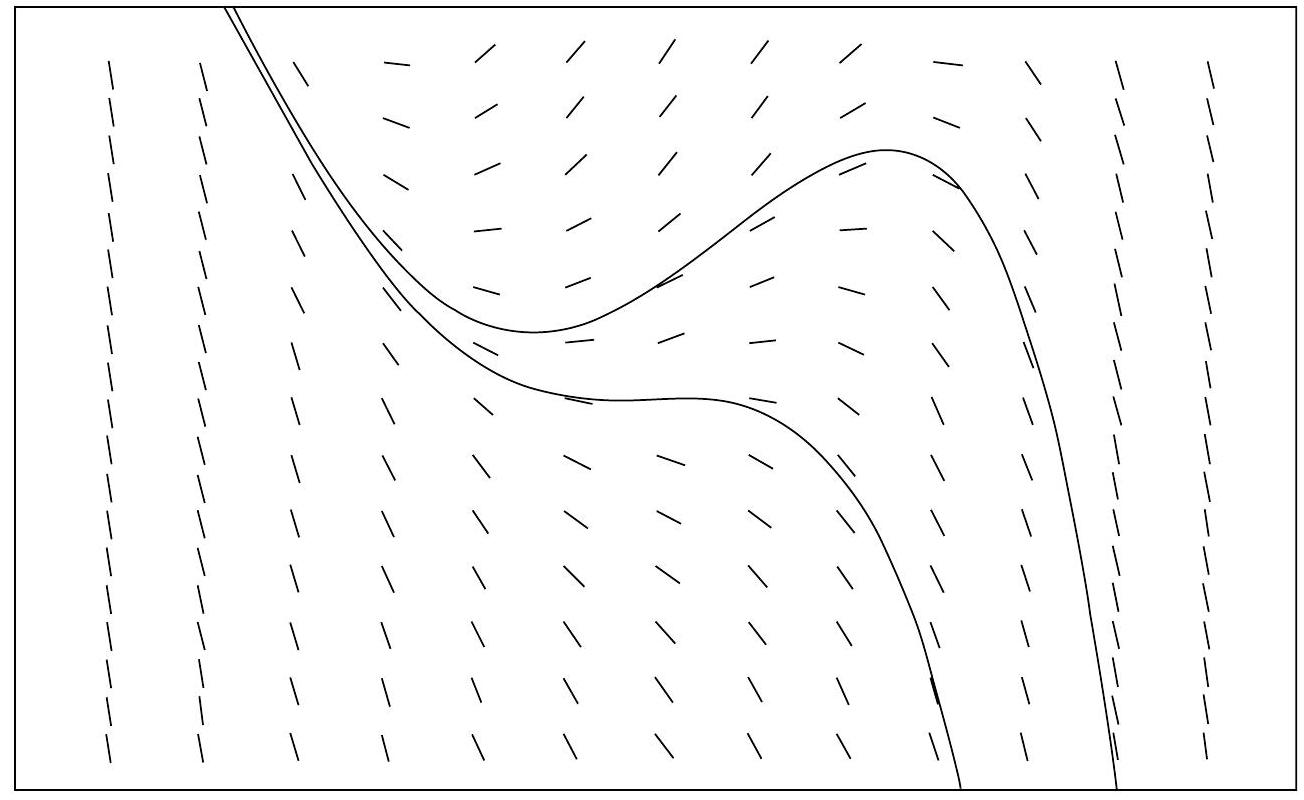
\includegraphics[max width=\textwidth]{2024_04_03_5bb5b4275a64cb9887d1g-371}
\end{center}

Fig. 18-20.

18.18. See Fig. 18-21.

\begin{center}
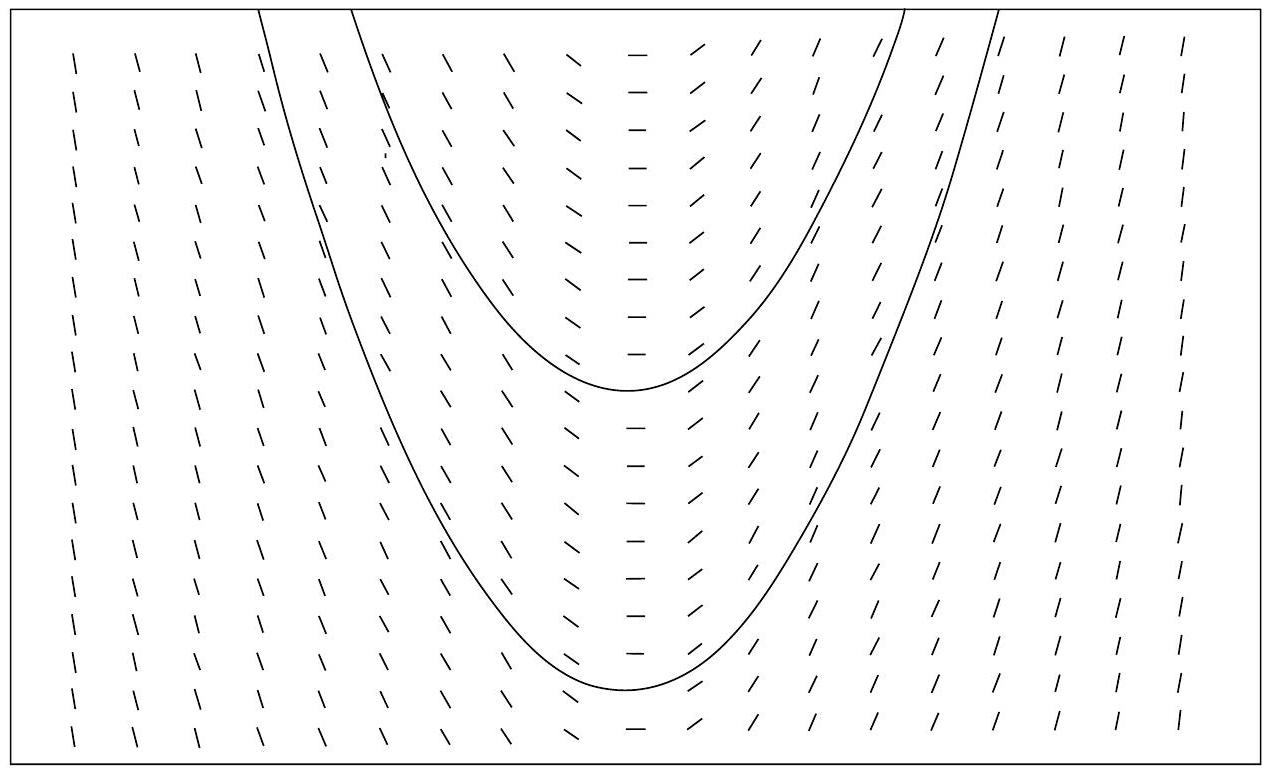
\includegraphics[max width=\textwidth]{2024_04_03_5bb5b4275a64cb9887d1g-372}
\end{center}

Fig. 18-21.

18.19. See Fig. 18-22.

\begin{center}
\includegraphics[max width=\textwidth]{2024_04_03_5bb5b4275a64cb9887d1g-372(1)}
\end{center}

Fig. 18-22.

18.20. See Fig. 18-23.

\begin{center}
\includegraphics[max width=\textwidth]{2024_04_03_5bb5b4275a64cb9887d1g-373}
\end{center}

Fig. 18-23.

18.21. See Fig. 18-24.

\begin{center}
\includegraphics[max width=\textwidth]{2024_04_03_5bb5b4275a64cb9887d1g-373(1)}
\end{center}

Fig. 18-24.

18.22. Four solution curves are drawn, beginning at the points $(1,3),(1,-3),(-1,-3)$, and $(-1,3)$, respectively, and continuing in the positive $x$-direction. See Fig. 18-25.

$\left[\begin{array}{lllllllllllllllllllllll}\hline 1 & 1 & 1 & 1 & 1 & 1 & 1 & 1 & 1 & 1 & 1 & 1 & 1 & 1 & 1 & 1 & 1 & 1 & 1 & 1 & 1 \\ 1 & 1 & 1 & 1 & 1 & 1 & 1 & 1 & 1 & 1 & 1 & 1 & 1 & 1 & 1 & 1 & 1 & 1 & 1 & 1 & 1 \\ 1 & 1 & 1 & 1 & 1 & 1 & 1 & 1 & 1 & 1 & 1 & 1 & 1 & 1 & 1 & 1 & 1 & 1 & 1 & 1 & 1 \\ 1 & 1 & 1 & 1 & 1 & 1 & 1 & 1 & 1 & 1 & 1 & 1 & 1 & 1 & 1 & 1 & 1 & 1 & 1 & 1 & 1 \\ 1 & 1 & 1 & 1 & 1 & 1 & 1 & 1 & 1 & 1 & 1 & 1 & 1 & 1 & 1 & 1 & 1 & 1 & 1 & 1 & 1 \\ 1 & 1 & 1 & 1 & 1 & 1 & 1 & 1 & 1 & 1 & 1 & 1 & 1 & 1 & 1 & 1 & 1 & 1 & 1 & 1 & 1 \\ 1 & 1 & 1 & 1 & 1 & 1 & 1 & 1 & 1 & 1 & 1 & 1 & 1 & 1 & 1 & 1 & 1 & 1 & 1 & 1 \\ 1 & 1 & 1 & 1 & 1 & 1 & 1 & 1 & 1 & 1 & 1 & 1 & 1 & 1 & 1 & 1 & 1 & 1 & 1 & 1 & 1 \\ 1 & 1 & 1 & 1 & 1 & 1 & 1 & 1 & 1 & 1 & 1 & 1 & 1 & 1 & 1 & 1 & 1 & 1 & 1 & 1 & 1 \\ 1 & 1 & 1 & 1 & 1 & 1 & 1 & 1 & 1 & 1 & 1 & 1 & 1 & 1 & 1 & 1 & 1 & 1 & 1 & 1 & 1 \\ 1 & 1 & 1 & 1 & 1 & 1 & 1 & 1 & 1 & 1 & 1 & 1 & 1 & 1 & 1 & 1 & 1 & 1 & 1 & 1 & 1 \\ 1 & 1 & 1 & 1 & 1 & 1 & 1 & 1 & 1 & 1 & 1 & 1 & 1 & 1 & 1 & 1 & 1 & 1 & 1 & 1 & 1 \\ 1 & 1 & 1 & 1 & 1 & 1 & 1 & 1 & 1 & 1 & 1 & 1 & 1 & 1 & 1 & 1 & 1 & 1 & 1 & 1 & 1 \\ 1 & 1 & 1 & 1 & 1 & 1 & 1 & 1 & 1 & 1 & 1 & 1 & 1 & 1 & 1 & 1 & 1 & 1 & 1 & 1 \\ 1 & 1 & 1 & 1 & 1 & 1 & 1 & 1 & 1 & 1 & 1 & 1 & 1 & 1 & 1 & 1 & 1 & 1 & 1 & 1 & 1 \\ 1 & 1 & 1 & 1 & 1 & 1 & 1 & 1 & 1 & 1 & 1 & 1 & 1 & 1 & 1 & 1 & 1 & 1 & 1 & 1 & 1 \\ 1 & 1 & 1 & 1 & 1 & 1 & 1 & 1 & 1 & 1 & 1 & 1 & 1 & 1 & 1 & 1 & 1 & 1 & 1 & 1 & 1 \\ 1 & 1 & 1 & 1 & 1 & 1 & 1 & 1 & 1 & 1 & 1 & 1 & 1 & 1 & 1 & 1 & 1 & 1 & 1 & 1 & 1 \\ 1 & 1 & 1 & 1 & 1 & 1 & 1 & 1 & 1 & 1 & 1 & 1 & 1 & 1 & 1 & 1 & 1 & 1 & 1 & 1 \\ 1 & 1 & 1 & 1 & 1 & 1 & 1 & 1 & 1 & 1 & 1 & 1 & 1 & 1 & 1 & 1 & 1 & 1 & 1 & 1 & 1\end{array}\right.$

Fig. 18-25.

18.23. See Fig. 18-17.

18.25. See Fig. 18-15.

18.27. See Fig. 18-16.

18.29. See Fig. 18-14.

18.31. See Fig. 18-18.\\
18.24. Straight lines of the form $y=x+(1-c)$

18.26. Vertical straight lines

18.28. Horizontal straight lines

18.30. Parabolas of the form $y=x^{2}+c$

18.32. Curves of the form $y=\sin x-c$

For comparison with other methods to be presented in subsequent chapters, answers are carried through $x=1.0$, and are given for additional values of $h$.

18.33.

\begin{center}
\includegraphics[max width=\textwidth]{2024_04_03_5bb5b4275a64cb9887d1g-375}
\end{center}

18.34.

\begin{center}
\includegraphics[max width=\textwidth]{2024_04_03_5bb5b4275a64cb9887d1g-375(1)}
\end{center}

18.35.

\begin{center}
\begin{tabular}{|c|c|c|c|c|}
\hline
\multicolumn{5}{|c|}{EULER'S METHOD} \\
\hline
\multicolumn{2}{|r|}{Problem:} & \multicolumn{3}{|c|}{$y^{\prime}=-y+x+2 ; y(0)=2$} \\
\hline
\multirow[t]{2}{*}{$x_{n}$} & \multicolumn{3}{|c|}{$y_{n}$} & \multirow{2}{*}{}\begin{tabular}{c}
True solution \\
$Y(x)=e^{-x}+x+1$ \\
\end{tabular} \\
\hline
 & $h=0.1$ & $h=0.05$ & $h=0.01$ &  \\
\hline
0.0 & 2.0000 & 2.0000 & 2.0000 & 2.0000 \\
\hline
0.1 & 2.0000 & 2.0025 & 2.0044 & 2.0048 \\
\hline
0.2 & 2.0100 & 2.0145 & 2.0179 & 2.0187 \\
\hline
0.3 & 2.0290 & 2.0351 & 2.0397 & 2.0408 \\
\hline
0.4 & 2.0561 & 2.0634 & 2.0690 & 2.0703 \\
\hline
0.5 & 2.0905 & 2.0987 & 2.1050 & 2.1065 \\
\hline
0.6 & 2.1314 & 2.1404 & 2.1472 & 2.1488 \\
\hline
0.7 & 2.1783 & 2.1877 & 2.1948 & 2.1966 \\
\hline
0.8 & 2.2305 & 2.2401 & 2.2475 & 2.2493 \\
\hline
0.9 & 2.2874 & 2.2972 & 2.3047 & 2.3066 \\
\hline
1.0 & 2.3487 & 2.3585 & 2.3660 & 2.3679 \\
\hline
\end{tabular}
\end{center}

18.36.

\begin{center}
\begin{tabular}{|c|c|c|c|c|}
\hline
 & Method: & \multicolumn{3}{|c|}{EULER'S METHOD} \\
\hline
 & Problem: & \multicolumn{3}{|c|}{$y^{\prime}=4 x^{3} ; y(0)=0$} \\
\hline
\multirow[t]{2}{*}{$x_{n}$} & \multicolumn{3}{|c|}{$y_{n}$} & \multirow{2}{*}{}\begin{tabular}{l}
True solution \\
$\qquad Y(x)=x^{4}$ \\
\end{tabular} \\
\hline
 & $h=0.1$ & $h=0.05$ & $h=0.01$ &  \\
\hline
0.0 & 0.0000 & 0.0000 & 0.0000 & 0.0000 \\
\hline
0.1 & 0.0000 & 0.0000 & 0.0001 & 0.0001 \\
\hline
0.2 & 0.0004 & 0.0009 & 0.0014 & 0.0016 \\
\hline
0.3 & 0.0036 & 0.0056 & 0.0076 & 0.0081 \\
\hline
0.4 & 0.0144 & 0.0196 & 0.0243 & 0.0256 \\
\hline
0.5 & 0.0400 & 0.0506 & 0.0600 & 0.0625 \\
\hline
0.6 & 0.0900 & 0.1089 & 0.1253 & 0.1296 \\
\hline
0.7 & 0.1764 & 0.2070 & 0.2333 & 0.2401 \\
\hline
0.8 & 0.3136 & 0.3600 & 0.3994 & 0.4096 \\
\hline
0.9 & 0.5184 & 0.5852 & 0.6416 & 0.6561 \\
\hline
1.0 & 0.8100 & 0.9025 & 0.9801 & 1.0000 \\
\hline
\end{tabular}
\end{center}

\section*{CHAPTER 19}
19.13.

\begin{center}
\begin{tabular}{|c|c|c|c|}
\hline
\multicolumn{3}{|c|}{Method: MODIFIED EULER'S METHOD} &  \\
\hline
\multicolumn{3}{|c|}{Problem: $y^{\prime}=-y+x+2 ; y(0)=2$} &  \\
\hline
$x_{n}$ & \multicolumn{2}{|c|}{$h=0.1$} & \multicolumn{1}{c|}{True solution} \\
\cline { 2 - 4 }
 & $p y_{n}$ & $y_{n}$ & $(x)=e^{-x}+x+1$ \\
\hline
0.0 & - & 2.000000 & 2.000000 \\
\hline
0.1 & 2.000000 & 2.005000 & 2.004837 \\
\hline
0.2 & 2.014500 & 2.019025 & 2.018731 \\
\hline
0.3 & 2.037123 & 2.041218 & 2.040818 \\
\hline
0.4 & 2.067096 & 2.070802 & 2.070320 \\
\hline
0.5 & 2.103722 & 2.107076 & 2.106531 \\
\hline
0.6 & 2.146368 & 2.149404 & 2.148812 \\
\hline
0.7 & 2.194463 & 2.197210 & 2.196585 \\
\hline
0.8 & 2.247489 & 2.249975 & 2.249329 \\
\hline
0.9 & 2.304978 & 2.307228 & 2.306570 \\
\hline
1.0 & 2.366505 & 2.368541 & 2.367879 \\
\hline
 &  &  &  \\
\hline
 &  &  &  \\
\hline
\end{tabular}
\end{center}

19.14.

\begin{center}
\begin{tabular}{|c|c|c|c|}
\hline
\multicolumn{4}{|c|}{MODIFIED EULER'S METHOD} \\
\hline
\multicolumn{4}{|c|}{Problem: $\quad y^{\prime}=-y ; y(0)=1$} \\
\hline
\multirow[t]{2}{*}{$x_{n}$} & \multicolumn{2}{|c|}{$h=0.1$} & \multirow{2}{*}{}\begin{tabular}{l}
True solution \\
$\qquad Y(x)=e^{-x}$ \\
\end{tabular} \\
\hline
 & $p y_{n}$ & $y_{n}$ &  \\
\hline
0.0 & - & 1.0000000 & 1.0000000 \\
\hline
0.1 & 0.9000000 & 0.9050000 & 0.9048374 \\
\hline
0.2 & 0.8145000 & 0.8190250 & 0.8187308 \\
\hline
0.3 & 0.7371225 & 0.7412176 & 0.7408182 \\
\hline
0.4 & 0.6670959 & 0.6708020 & 0.6703201 \\
\hline
0.5 & 0.6037218 & 0.6070758 & 0.6065307 \\
\hline
0.6 & 0.5463682 & 0.5494036 & 0.5488116 \\
\hline
0.7 & 0.4944632 & 0.4972102 & 0.4965853 \\
\hline
0.8 & 0.4474892 & 0.4499753 & 0.4493290 \\
\hline
0.9 & 0.4049777 & 0.4072276 & 0.4065697 \\
\hline
1.0 & 0.3665048 & 0.3685410 & 0.3678794 \\
\hline
\end{tabular}
\end{center}

19.15.

\begin{center}
\begin{tabular}{|c|c|c|c|}
\hline
\multicolumn{3}{|c|}{Method: ${ }^{2}$ MODIFIED EULER'S METHOD} &  \\
\hline
\multicolumn{2}{|c|}{Problem: $y^{\prime}=\frac{x^{2}+y^{2}}{x y} ; y(1)=3$} &  &  \\
\cline { 1 - 4 }
$x_{n}$ & \multicolumn{2}{|c|}{$h=0.2$} & \multirow{2}{*}{True solution} \\
\cline { 2 - 4 }
 & $p y_{n}$ & $y_{n}$ &  \\
\hline
1.0 & - & 3.0000 & 3.0000 \\
\hline
1.2 & 3.6667 & 3.6716 & 3.6722 \\
\hline
1.4 & 4.3489 & 4.3530 & 4.3542 \\
\hline
1.6 & 5.0393 & 5.0429 & 5.0444 \\
\hline
1.8 & 5.7367 & 5.7399 & 5.7419 \\
\hline
2.0 & 6.4404 & 6.4432 & 6.4456 \\
\hline
\end{tabular}
\end{center}

19.16. The true solution is $Y(x)=x^{2} / 2-1$, a second-degree polynomial. Since the modified Euler's method is a secondorder method, it will generate the exact solution.

19.17.

\begin{center}
\begin{tabular}{|c|c|c|c|}
\hline
\multicolumn{3}{|c|}{Method: MODIFIED EULER'S METHOD} &  \\
\hline
\multicolumn{3}{|c|}{Problem: $y^{\prime}=-4 x^{3} ; y(2)=6$} &  \\
\hline
\multirow{2}{*}{$x_{n}$} & \multicolumn{2}{|c|}{$h=0.2$} & \multirow{2}{*}{}\begin{tabular}{l}
$Y(x)=x^{4}-10$ \\
\end{tabular} \\
\cline { 2 - 4 }
 & $p y_{n}$ & $y_{n}$ &  \\
\hline
2.0 & - & 6.0000 & 13.4256 \\
\hline
2.2 & 12.4000 & 13.4592 & 23.1776 \\
\hline
2.4 & 21.9776 & 23.2480 & 35.6976 \\
\hline
2.6 & 34.3072 & 35.8080 & 51.4656 \\
\hline
2.8 & 49.8688 & 51.6192 & 71.0000 \\
\hline
3.0 & 69.1808 & 71.2000 &  \\
\hline
\end{tabular}
\end{center}

19.18.

\begin{center}
\begin{tabular}{|c|c|c|}
\hline
\multicolumn{3}{|c|}{Method:} \\
\hline
\multicolumn{2}{|c|}{RUNGE-KUTTA METHOD} &  \\
\hline
$x_{n}$ & \begin{tabular}{c}
$h=0.1$ \\
$y_{n}$ \\
\end{tabular} & \begin{tabular}{c}
True solution \\
$Y(x)=e^{-x}+x+1$ \\
\end{tabular} \\
\hline
0.0 & 2.000000 & 2.000000 \\
\hline
0.1 & 2.004838 & 2.004837 \\
\hline
0.2 & 2.018731 & 2.018731 \\
\hline
0.3 & 2.040818 & 2.040818 \\
\hline
0.4 & 2.070320 & 2.070320 \\
\hline
0.5 & 2.106531 & 2.106531 \\
\hline
0.6 & 2.148812 & 2.148812 \\
\hline
0.7 & 2.196586 & 2.196585 \\
\hline
0.8 & 2.249329 & 2.249329 \\
\hline
0.9 & 2.306570 & 2.306570 \\
\hline
1.0 & 2.367880 & 2.367879 \\
\hline
 &  &  \\
\hline
\end{tabular}
\end{center}

19.19.

\begin{center}
\begin{tabular}{|c|c|c|}
\hline
\multicolumn{2}{|c|}{Method:} & RUNGE-KUTTA METHOD \\
\hline
\multicolumn{2}{|c|}{Problem: $y^{\prime}=-y ; y(0)=1$} &  \\
\hline
$x_{n}$ & \begin{tabular}{c}
$h=0.1$ \\
$y_{n}$ \\
\end{tabular} & \begin{tabular}{c}
True solution \\
$Y(x)=e^{-x}$ \\
\end{tabular} \\
\hline
0.0 & 1.0000000 & 1.0000000 \\
\hline
0.1 & 0.9048375 & 0.9048374 \\
\hline
0.2 & 0.8187309 & 0.8187308 \\
\hline
0.3 & 0.7408184 & 0.7408182 \\
\hline
0.4 & 0.6703203 & 0.6703201 \\
\hline
0.5 & 0.6065309 & 0.6065307 \\
\hline
0.6 & 0.5488119 & 0.5488116 \\
\hline
0.7 & 0.4965856 & 0.4965853 \\
\hline
0.8 & 0.4493293 & 0.4493290 \\
\hline
0.9 & 0.4065700 & 0.4065697 \\
\hline
1.0 & 0.3678798 & 0.3678794 \\
\hline
\end{tabular}
\end{center}

19.20.

\begin{center}
\begin{tabular}{|c|c|c|}
\hline
\multicolumn{3}{|c|}{Method:} \\
\hline
\multicolumn{2}{|c|}{RUNGE-KUTTA METHOD} &  \\
\hline
$x_{n}$ & \begin{tabular}{c}
$h=0.2$ \\
$y_{n}$ \\
\end{tabular} & \begin{tabular}{c}
True solution \\
$Y(x)=x \sqrt{9+\ln x^{2}}$ \\
\end{tabular} \\
\hline
1.0 & 3.0000000 & 3.0000000 \\
\hline
1.2 & 3.6722028 & 3.6722045 \\
\hline
1.4 & 4.3541872 & 4.3541901 \\
\hline
1.6 & 5.0444406 & 5.0444443 \\
\hline
1.8 & 5.7418469 & 5.7418514 \\
\hline
2.0 & 6.4455497 & 6.4455549 \\
\hline
\end{tabular}
\end{center}

19.21. Since the true solution $Y(x)=x^{4}-10$ is a fourth-degree polynomial, the Runge-Kutta method, which is a fourthorder numerical method, generates an exact solution.

19.22.

\begin{center}
\begin{tabular}{|c|c|c|}
\hline
\multicolumn{2}{|c|}{Method:} & RUNGE-KUTTA METHOD \\
\hline
\multicolumn{2}{|c|}{Problem: $y^{\prime}=5 x^{4} ; y(0)=0$} &  \\
\hline
$x_{n}$ & \begin{tabular}{c}
$h=0.1$ \\
$y_{n}$ \\
\end{tabular} & \begin{tabular}{c}
True solution \\
$Y(x)=x^{5}$ \\
\end{tabular} \\
\hline
0.0 & 0.0000000 & 0.0000000 \\
\hline
0.1 & 0.0000104 & 0.0000100 \\
\hline
0.2 & 0.0003208 & 0.0003200 \\
\hline
0.3 & 0.0024313 & 0.0024300 \\
\hline
0.4 & 0.0102417 & 0.0102400 \\
\hline
0.5 & 0.0312521 & 0.0312500 \\
\hline
0.6 & 0.0777625 & 0.0777600 \\
\hline
0.7 & 0.1680729 & 0.1680700 \\
\hline
0.8 & 0.3276833 & 0.3276800 \\
\hline
0.9 & 0.5904938 & 0.5904900 \\
\hline
1.0 & 1.0000042 & 1.0000000 \\
\hline
\end{tabular}
\end{center}

\begin{center}
\begin{tabular}{|c|c|c|c|}
\hline
\multicolumn{4}{|c|}{Method: ADAMS-BASH} \\
\hline
\multicolumn{4}{|c|}{Problem: $y^{\prime}=y ; y(0)=1$} \\
\hline
\multirow[t]{2}{*}{$x_{n}$} & \multicolumn{2}{|c|}{$h=0.1$} & \multirow{2}{*}{}\begin{tabular}{l}
True solution \\
$\qquad Y(x)=e^{-x}$ \\
\end{tabular} \\
\hline
 & $p y_{n}$ & $y_{n}$ &  \\
\hline
0.0 & - & 1.0000000 & 1.0000000 \\
\hline
0.1 & - & 1.1051708 & 1.1051709 \\
\hline
0.2 & - & 1.2214026 & 1.2214028 \\
\hline
0.3 & - & 1.3498585 & 1.3498588 \\
\hline
0.4 & 1.4918201 & 1.4918245 & 1.4918247 \\
\hline
0.5 & 1.6487164 & 1.6487213 & 1.6487213 \\
\hline
0.6 & 1.8221137 & 1.8221191 & 1.8221188 \\
\hline
0.7 & 2.0137473 & 2.0137533 & 2.0137527 \\
\hline
0.8 & 2.2255352 & 2.2255418 & 2.2255409 \\
\hline
0.9 & 2.4595971 & 2.4596044 & 2.4596031 \\
\hline
1.0 & 2.7182756 & 2.7182836 & 2.7182818 \\
\hline
\end{tabular}
\end{center}

19.24.

\begin{center}
\begin{tabular}{|c|c|c|c|}
\hline
\multicolumn{4}{|c|}{Problem: $y^{\prime}=-y+x+2 ; y(0)=2$} \\
\hline
\multirow[t]{2}{*}{$x_{n}$} & \multicolumn{2}{|c|}{$h=0.1$} & \multirow{2}{*}{}\begin{tabular}{c}
True solution \\
$Y(x)=e^{-x}+x+1$ \\
\end{tabular} \\
\hline
 & $p y_{n}$ & $y_{n}$ &  \\
\hline
0.0 & - & 2.000000 & 2.000000 \\
\hline
0.1 & - & 2.004838 & 2.004837 \\
\hline
0.2 & - & 2.018731 & 2.018731 \\
\hline
0.3 & - & 2.040818 & 2.040818 \\
\hline
0.4 & 2.070323 & 2.070320 & 2.070320 \\
\hline
0.5 & 2.106533 & 2.106530 & 2.106531 \\
\hline
0.6 & 2.148814 & 2.148811 & 2.148812 \\
\hline
0.7 & 2.196587 & 2.196585 & 2.196585 \\
\hline
0.8 & 2.249330 & 2.249328 & 2.249329 \\
\hline
0.9 & 2.306571 & 2.306569 & 2.306570 \\
\hline
1.0 & 2.367880 & 2.367878 & 2.367879 \\
\hline
\end{tabular}
\end{center}


\end{document}